% \NeedsTeXFormat{LaTeX2e}
%-----------------------------------------------------------------------------
% To run master file, doc_mra.tex: 
% rm *.aux (to remove previous links/cross-references)
%
% comments INC 2 and INC 3, and uncomment INC 1
% latex doc_mra
% comments INC 1 and INC 3, and uncomment INC 2
% latex doc_mra
% comments INC 1 and INC 2, and uncomment INC 3
% latex doc_mra

% Apply bibtex
% bibtex doc_mra

% comments INC 2 and INC 3, and uncomment INC 1
% latex doc_mra
% latex doc_mra
% dvips doc_mra -l 193 -o doc_vol1.ps
% comments INC 1 and INC 3, and uncomment INC 2
% latex doc_mra
% latex doc_mra
% dvips doc_mra -p 195 -o  doc_vol2.ps
% comments INC 1 and INC 2, and uncomment INC 3
% latex doc_mra
% latex doc_mra
% dvips doc_mra -o doc_vol3.ps
%
% Problem index: when compile parts of the documentation, the \makeindex command
% remove the file doc_mra.idx which contains the index  relative to the 
% other part of the documentation:
% A solution:
% ----------
%   Compile Part 1: and save makeindex doc_mra.idx  in I1
%   Compile Part 2: and save makeindex doc_mra.idx  in I2
%   Compile Part 3: and save makeindex doc_mra.idx  in I3
%   mv I1 doc_mra.idx
%   cat I2 >> doc_mra.idx
%   cat I3 >> doc_mra.idx
%   comments the line  \makeindex in this file
%   recompile the three parts

% J.-L. Starck, APRIL 1999
%-----------------------------------------------------------------------------

\documentclass[11pt,a4paper,titlepage]{book}
% \usepackage{psfig,amstex,amssymb,alltt,makeidx}
\usepackage{psfig}
\usepackage{amssymb,alltt}
\usepackage{amsmath}
\usepackage{latexsym}
\usepackage{graphicx}
\usepackage{makeidx}
% \usepackage{supertab}
% \usepackage{longtable}
% \usepackage{amssymb,alltt,makeidx}
% \usepackage{chapterbib}
% \usepackage{bibunits}

% \makeindex

\newcommand{\mr}{./doc_mr1}
\newcommand{\mw}{./doc_mr2}
\newcommand{\psdir}{/home/starck/tex/report/FIG}
\newcommand{\mc}{./doc_mr3}
\newcommand{\cur}{./doc_mr4}

\psfigurepath{\psdir/deconv:\psdir/prediction:\psdir/filter_xima:\psdir/contrast:\psdir/curvelet:\psdir/cf_ana:\psdir/mchannel:\psdir/mr1:\psdir/demo:\psdir/cours:\psdir/edge:\psdir/compress:\psdir/fractal:\psdir/detect:\psdir/book98:\psdir/entropy:\psdir/iso:\psdir/cours}

\def\aa{{A\&A } }
\def\aj{{AJ} }
\def\apj{{ApJ\ }}
\def\va{{ Vistas in Astronomy}}
\def\pasp{{ PASP\ }}

\def\projmra{MR}
\def\defprojmra{The Multiresolution Analysis Software}

\medskip

\def\proj{MR/1 }
\def\defproj{The Multiresolution Environment}

\def\projmw{MR/2 }
\def\defprojmw{Multiscale Entropy and Applications}

\def\projmc{MR/3 }
\def\projmr3{MR/3 }
\def\defprojmc{Multichannel Data}

\def\projcur{MR/4 }
\def\defprojcur{Ridgelets and Curvelets}

\newcommand{\be}{\begin{eqnarray}}
\newcommand{\ee}{\end{eqnarray}}
\newcommand{\bn}{\begin{enumerate}}
\newcommand{\en}{\end{enumerate}}
\newcommand{\bi}{\begin{itemize}}
\newcommand{\ei}{\end{itemize}}
\newcommand{\mmin}{\wedge}
\newcommand{\mmax}{\vee}  
\newcommand{\bmmin}{\bigwedge} 
\newcommand{\bmmax}{\bigvee}   
\newtheorem{theorem}{Theorem}
\newtheorem{lemma}[theorem]{Lemma}
\newtheorem{corollary}[theorem]{Corollary}
\newtheorem{proposition}[theorem]{Proposition}
\newtheorem{definition}[theorem]{Definition}
\newcommand{\goto}{\rightarrow}
\newcommand{\bitem}{\begin{itemize}}
\newcommand{\eitem}{\end{itemize}}
\newcommand{\bR}{{\bf R}}
\newcommand{\eps}{{\epsilon}}
\newcommand{\cR}{{\cal R}}
\newcommand{\cQ}{{\cal Q}}
\newcommand{\cW}{{\mathcal W}}
\newcommand{\cA}{{\mathcal A}}
\newcommand{\cP}{{\mathcal P}}
\newcommand{\cS}{{\mathcal S}}
\newcommand{\bZ}{{\bf Z}}
\newcommand{\cM}{{\cal M}}
\newcommand{\<}{\langle}
\renewcommand{\>}{\rangle}
\newcommand{\qed}{\quad\hbox{\vrule width 4pt height 6pt depth 1.5pt}}
\newcommand{\cH}{{\cal H}}
\newcommand{\cL}{{\cal L}}


\textwidth 16truecm
\textheight 23truecm
\hoffset -1.5truecm
\voffset -0.5truecm


% \makeindex
% \input psfig.tex

% \voffset -1.5cm
% \hoffset -1.cm
\evensidemargin 1.truecm
\oddsidemargin  1.truecm

%\title{{\bf \Huge \projmra: \defprojmra }  \\
%\title{{\bf \Huge The Multiresolution Analysis Software: }\\
%$ $ \\
%  {\Large \bf \mbox{MR/1 -- Environment:   version 4.0}}  
%%  {\Large \bf \mbox{MR/2 -- Entropy:       version 1.2}}  
%  {\Large \bf \mbox{MR/3 -- 3D and Multi-channel: version 2.0}}
%  {\Large \bf \mbox{MR/4 -- Ridgelet-Curvelet: version 1.0}}}
% $ $ \\
% $ $ \\ {\large Technical Report} }
% \vspace{0.2cm}

\author{CEA-SACLAY/SEDI-SAP}
 
 \date{  \begin{figure}[hb]
\centerline{
\hbox{
% \psfig{figure=fig_ngc.ps,bbllx=1.9cm,bblly=12.6cm,bburx=14.6cm,bbury=25.4cm,width=9cm,height=9cm,clip=}
\psfig{figure=ch2_wave_synt.ps,bbllx=3cm,bblly=10.6cm,bburx=18.6cm,bbury=26.3cm,width=10cm,height=10cm,clip=}
}}
\end{figure}
} 

 
% \includeonly{part1,cover,\mr/ch1_intro,\mr/ch3_prog,\mr/ch4_wave,\mr/ch_restore,\mr/ch_compress,\mr/ch_detect,\mr/ch_register,\mr/ch_edge,\mr/ch_1d,\mr/ch_time,\mr/ch_fractal,\mr/ch5_idl,\mr/annex_lifting,\mr/annex_packet,\mr/annex_wavemed}
% \includeonly{part2,\mw/intro,\mw/concept,\mw/filter,\mw/deconv,\mw/fluctu,\mw/prog,\mw/mr2_idl,\mw/annexA,\mw/annex_noise,\mw/annex_deriv1,\mw/annex_deriv2}
% \includeonly{part3,\mc/mc_tools,\mc/data_3d,\mc/mc_3d}
% \includeonly{part4,\cur/ch_curvelet,\cur/ch_curfilter,\cur/ch_combfilter,\cur/ch_curcontrast,\cur/ch_curprog,partbib}

\begin{document}

\maketitle
\newpage
$ $ 
\newpage
{\large
\voffset 0cm
\pagenumbering{roman}
\addcontentsline{toc}{chapter}{Contents}
\tableofcontents

 
\pagenumbering{arabic}
\clearpage


\part{\projmrs: \defprojmrs}

 
\chapter{Introduction}
\label{ch_intro}
% \chapterhead{Introduction}
\markright{Introduction}

% \proj (\defproj) 
\proj is a
set of software components 
developed by CEA (Saclay, France) and Nice Observatory. This
project originated in astronomy, and involved the development of a range of 
innovative methods built around multiscale analysis.
Multiresolution techniques have
been developed  in recent years, and furnish a powerful and 
insightful representation
of the data. By means of multiresolution or multiscale analysis, an 
image can be decomposed into a set of images (or scales), each scale 
containing only structures of a given size. 
This data representation, associated with noise modeling, 
has been applied to very different applications such as data filtering, 
deconvolution, compression, object detection, and so on. Results are 
enhanced in all such processing because the multiresolution approach
allows a better understanding of how the data values 
are distributed in an image, 
and how the signal can be separated from the noise.

The \proj software 
components include almost all applications 
presented in the book {\em Image and Data Analysis: the Multiscale Approach}
 \cite{starck:book98}. The goal of 
\proj is not to replace 
existing image processing  packages, but to complement
them, offering the user a complete set of multiresolution tools. These tools
are executable programs, which work on a wide range of platforms, 
independently of current 
image processing systems.  They allow the user to perform various tasks 
using multiresolution, such as wavelet transforms, filtering, 
deconvolution, and so on.

The programs, written in C++, are built on three classes: the  
``image" class, the ``multiresolution" class, and the 
``noise\_modeling class".
Fig. \ref{fig_sadam1} illustrates this architecture. A multiresolution
transform is applied to the input data, and noise modeling is performed.
Hence the multiple scales  can be derived, and the programs can use this
in order to know at which scales, and at which positions, significant
signal has been detected. 
A wide range of 
multiresolution transforms are available (see Fig.~\ref{fig_sadam2}),
allowing significant flexibility.
Fig.\ \ref{fig_modelnoise} summarizes how the multiresolution support data
structure 
is derived from the data and the noise-modeling. 


A set of  IDL\footnote{Research Systems 
Inc., 2995 Wilderness Place, Boulder, Colorado 80301.} (Interactive 
Data Language) 
and PV$\sim$Wave\footnote{Visual Numerics Inc.,  6230 Lookout Road, 
Boulder, Colorado 80301, USA.}
routines
are included in the package which interface the executables to these
image processing packages.  

\proj is an important package, 
introducing front-line methods to scientists 
in the physical, space and medical domains among other fields; to engineers in 
such disciplines as geology and electrical engineering; and to financial 
engineers and those in  other fields requiring control and analysis of 
large quantities of noisy data.  

% The first release of the package is at the 
% beginning of 1997.  
% Further information on the pre-release version, codenamed 
% \proj, can be found at  \\ 
% http://www.dapnia.cea.fr/Sadam

\begin{figure}[t]
\centerline{
\hbox{
\psfig{figure=ch_annex2_sadam.ps,bbllx=2.5cm,bblly=3.cm,bburx=17.5cm,bbury=25cm,height=12cm,width=12cm,clip=}
}}
\caption{\proj diagram.}
\label{fig_sadam1}
\end{figure}

\begin{figure}[htb]
\centerline{
\hbox{
% \psfig{figure=ch_annex2_mr_trans.ps,bbllx=0.5cm,bblly=3.5cm,bburx=20.5cm,bbury=24.5cm,height=16cm,width=15cm,clip=}
\psfig{figure=fig_mr1_transf.ps,bbllx=0.2cm,bblly=3.5cm,bburx=20.5cm,bbury=24.5cm,height=16cm,width=15cm,clip=}
}}
\caption{Multiresolution transforms available in \proj (a selection).}
\label{fig_sadam2}
\end{figure}

\begin{figure}[htb]
\centerline{
\hbox{
\psfig{figure=ch2_noise.ps,bbllx=0.5cm,bblly=1.5cm,bburx=22cm,bbury=26.5cm,width=13cm,height=16.66cm,clip=}}
}
\caption{Determination of multiresolution support from noise modeling.}
\label{fig_modelnoise}
\index{multiresolution support}
\index{support, multiresolution}
\end{figure}

%  
\chapter{Installation}
\label{ch_install}
% \chapterhead{Installation}
 
\textbf{IMPORTANT!} Before going any further, please read and accept the terms
in the file COPYRIGHT.


\section{Download}

To install MR/1 on your system you need the MR-install script and 
a distribution file.


\subsection{Distribution files}

First you have to choose the distribution of MR/1 binaries appropriate to your
host's system.

\vspace{0.3cm}
{\centering \begin{tabular}{|c|c|}
\hline 
Identification&
Host System\\
\hline 
\hline 
alpha\_osf&
Alpha (DEC) running OSF/1\\
\hline 
hp\_ux\_09&
HP 9000 series 700 or 800 or HP UX 10.x\\
\hline 
i486\_linuxlibc2&
Intel x86 Linux libc2 '99 distributions\\
\hline 
rs6000\_ibm\_aix&
IBM RS/6000 \\
\hline 
sun4x\_5.6&
Sun 4 Sparc or Ultra running Solaris 2.6\\
\hline 
i586\_cygwin32 & Windows 95,98, and NT\\
\hline
\end{tabular}\par}
\vspace{0.3cm}

For each system (xx\_xx is the identification of your host system), 4 gzip'ed
tar archives are provided:

\begin{itemize}
\item MR\-3.0\-xx\_xx.tgz contains all the MR/1,MR/2, and MR/3 executables
\item cea\_lm-3.0-xx\_xx.tgz contains the binary of the floating licence server
\item mr\_decomp-3.0-xx\_xx.tgz and mr\_upresol-3.0-xx\_xx.tgz contain 
the decompression utilities
\end{itemize}

A set of IDL routines (for IDL Version 5) is also available in the
file idlv5.tar.gz, allowing the executables to be called directly from IDL.

\subsection{Example}

If you wish to run MR/1 on IBM, you will need the following files:

\begin{itemize}
\item MR-3.0-rs6000\_ibm\_aix.tgz,
\item cea\_lm-3.0-rs6000\_ibm\_aix.tgz.
\end{itemize}

\subsection{Installation}

To proceed, you need to have: the MR-install script and the distribution
archive. During the installation procedure, you will be asked for an 
installation
directory (with writable authorization and enough available space) and licence
information dedicated to your host (hostname and hostid).

If you plan to install only the decompression utility, you do not need any 
licence.

This table gives the maximum space needed to fully install 
MR/1 on various systems:

\vspace{0.3cm}
{\centering \begin{tabular}{|c|c|}
\hline 
Alpha &
200 MB\\
\hline 
HP &
128 MB\\
\hline 
Linux &
140 MB\\
\hline 
IBM RS/6000&
330 MB\\
\hline 
Sun Solaris 2.5&
120 MB\\
\hline 
WINDOWS 95, 98, and NT &
225 MB\\
\hline 
\end{tabular}\par}
\vspace{0.3cm}

MR-install is a shell script which will help to easily extract the binaries
from the distribution archive and to configure the licence server.

If you get the distribution using Internet (i.e., ftp), you will have to 
check the file permission
of the shell script MR-install. ``\textsl{chmod +x MR-install}''
may be needed to add execute permission.

Ater running this script, \textsl{./MR-install}, you
will need to modify the \textsl{PATH} system variable to include
the installation directory. You may ask your system administrator to modify
your host so that it will automatically start the licence manager 
whenever you reboot your computer.

Once everything is fine, you can remove the MR-install script and 
the distribution archive from your host.


\subsection{How to start?}

The directory with executables corresponding to the selected
type of computers must be in the user path.  
The licence manager can be run (if not already done so by your system manager)
by typing 
\begin{center}
 {\bf cea\_lm -file fileName}
 \end{center}
 or directly {\bf cea\_lm} if the default file name has been chosen. 

For non-floating licences, the programs
can only be executed on the computer where the  licence manager is installed.
For floating licences, the programs can be run from any computer (with the 
correct type of platform) on the network 
if the environment variable {\bf CEA\_LICENSE\_HOST} is set 
to the correct address (for example ariane.saclay.cea.fr), or if the licence file is 
in the directory {\bf /usr/local/cea} (and {\bf  C:\verb+\+Program Files\verb+\+MR} for WINDOWS).

When the licence manager is running, all executables described in 
this document can be called.

\subsection{JAVA Interface}
 
\subsubsection*{Required packages}
\begin{itemize}
\item JDK1.2. (http://java.sun.com/products/index.html)
\item Swing1.1. (http://java.sun.com/products/index.html)
\item MR/1 interface Java class (mr.class, ....)
\end{itemize} 

\subsubsection*{Running MR Java application}

On unix computers, the {\bf CLASSPATH} variable must contain the Java class 
directory and the Swing class directory. \\ 
Run the program by typing:
\begin{verbatim}
> java mr
\end{verbatim}

On WINDOWS, run the program by typing:
\begin{verbatim}
> jmr1
\end{verbatim}
if the default installation directory has been choosen. Otherwise you
will have to edit the jmr1.bat file, and modify the variable accordingly
to your installation.

If the license manager is not running, it has to be started from the 
menu ``System''$>$``cea\_lm...'', by selecting the ``Status'' option.


Exit the program by selecting ``Quit...'' in the ``System'' menu.
\begin{verbatim}
"System">"Quit..."
\end{verbatim}
The license manager can be stopped before from the 
menu ``System''$>$11cea\_lm...'', by selecting the ``Kill'' option.

\subsubsection*{Description}

The MR/1 graphical user inteface allows the user to execute all the MR/1  
programs.
The application window contains a menu bar with 5 tear-off menus: 
\begin{itemize}
\item System: quit, and licence manipulation.
\item MR/1 IMAGE: image manipulation programs (multiresolution not used).
\item MR/1 Multiresol: manipulation of multiresolution objects.
\item MR/1 Application: filtering, deconvolution, compression, detection, etc.
\item MR/1 1D: 1D programs.
\end{itemize}
To execute an MR program select the associated item (program name): \\
``MR/1 Image'' $>$ ``Manipulation tools'' $>$ ``im\_info'', 
for the im\_info program.  

The application displays a popup window. All the options of the 
program can be
selected. If a popup window is validated (by pressing the  
OK button) with an obligatory 
option not initialized, a warning dialog box prevents the user continuing.

When the dialog box is validated the programm is executed. 
Information on the execution is displayed in the current window: 
\begin{verbatim}
  Program is running ...
  ... information relative to the program execution ...
  Program is finished!
The execution is now terminated.
\end{verbatim}

The help button of the dialog box displays a window with the help of the 
program.


\subsection{IDL routines}

To use IDL routines, the {\bf CEA\_MR\_DIR} variable 
must be initialized to the directory
where the MR/1-IDL software has been installed. Then 
the command
\begin{center}
{\bf idl \$CEA\_MR\_DIR/idl/pro/mre} 
\end{center}
runs the IDL session with the 
multiresolution environment. An IDL help facility on the available routines
is obtained by typing {\bf mrh} in the IDL session. 






 

\chapter{\proj Image Processing Tools}
\label{ch_prog}
% \chapterhead{Programs}
\markright{Image Processing Tools}

% \section{General information}
% \textbf{IMPORTANT!} Before going any further, please read and accept the terms
% in the file COPYRIGHT.

\section{Introduction}

\subsection{License manager: cea\_lm}
\index{cea\_lm}
The directory with executables must be in the user path.  
The license manager can be run (if not already done so by your system manager)
by typing 
\begin{center}
 {\bf cea\_lm -file fileName}
 \end{center}
 or directly {\bf cea\_lm} if the default file name, {\bf cea\_lic}, is 
used. The license manager can be stopped before  by typing 
\begin{center}
 {\bf cea\_lm -kill}
 \end{center} 

For non-floating licenses, the programs
can only be executed on the computer where the  license manager is installed.\\
For floating licenses, the programs can be run from any computer (with the 
correct type of platform) on the network 
if the environment variable {\bf CEA\_LICENSE\_HOST} \index{CEA\_LICENSE\_HOST}
is set 
to the correct address (for example ariane.saclay.cea.fr), 
or if the license file is 
in the directory {\bf /usr/local/cea} 
(and {\bf  C:\verb+\+Program Files\verb+\+MR} for Windows 95/98/NT/ME, \dots).

When the license manager is running, all executables described in 
this document can be called.

\subsection{JAVA interface}
 
\subsubsection*{Required packages}
\begin{itemize}
\item JDK (http://java.sun.com/products/index.html), at least version $1.2$.
\item Swing (http://java.sun.com/products/index.html), 
at least version $1.1$. With recent JDK versions, Swing is 
included.
\item MR/1 interface Java class (mr.class, ....)
\end{itemize} 

\subsubsection*{Running the MR Java application}

On Unix computers, the {\bf CLASSPATH} variable must contain the Java class 
directory and the Swing class directory. \\ 
Run the program by typing:
\begin{verbatim}
> java mr
\end{verbatim}

On Windows, run the program by typing:
\begin{verbatim}
> jmr1
\end{verbatim}
if the default installation directory has been chosen. Otherwise you
will have to edit the jmr1.bat file, and modify the path variables according
to your installation.

% If the license manager is not running, it has to be started from the 
% menu ``System''$>$``cea\_lm...'', by selecting the ``Status'' option.


Exit the program by selecting ``Quit...'' in the ``System'' menu.
\begin{verbatim}
"System">"Quit..."
\end{verbatim}
% The license manager can be stopped before from the 
% menu ``System''$>$ ``cea\_lm...'', by selecting the ``Kill'' option.

\subsubsection*{Description}

The MR/1 graphical user interface allows the user to execute all the MR/1  
programs.
The application window contains a menu bar with 5 tear-off menus: 
\begin{itemize}
\item System: quit, and license manipulation.
\item MR/1 IMAGE: image manipulation programs (multiresolution not used).
\item MR/1 Multiresol: manipulation of multiresolution objects.
\item MR/1 Application: filtering, deconvolution, compression, detection, etc.
\item MR/1 1D: 1D programs.
\item MR/2: MR/2 programs.
\item MR/3: MR/3 programs.
\item MR/4: MR/4 programs.
\end{itemize}
To execute an MR program select the associated item (program name): \\
``MR/1 Image'' $>$ ``Manipulation tools'' $>$ ``im\_info'', 
for the im\_info program.  

The application displays a popup window. All the options of the 
program can be
selected. If a popup window is validated (by pressing the  
OK button) with an obligatory 
option not initialized, a warning dialog box prevents the user continuing.

When the dialog box is validated the program is executed. 
Information on the execution is displayed in the current window: 
\begin{verbatim}
  Program is running ...
  ... information relative to the program execution ...
  Program is finished!
The execution is now terminated.
\end{verbatim}

The help button of the dialog box displays a window with the help of the 
program.


\subsection{IDL routines}

To use IDL routines, the {\bf CEA\_MR\_DIR} \index{CEA\_MR\_DIR} variable 
must be initialized to the directory
where the MR/1-IDL software has been installed. Then 
the command
\begin{center}
{\bf idl \$CEA\_MR\_DIR/idl/pro/mre} 
\end{center}
runs the IDL session with the 
multiresolution environment. An IDL help facility on the available routines
is obtained by typing {\bf mrh} in the IDL session. 


\section{Image Format}
\index{format}
All programs read/write to raw format (.d), FITS format (.fits), 
GIF format (.gif), JPEG format (.jpg) and PGM format (.pgm). 
A raw image file name must have the 
following syntax:  FileName\_x\_Nl\_Nc.d \\
 where x defines the data type: 
\begin{verbatim}
                          x = b (byte)
                              s (short int)
                              i (int)
                              f (float)
                              d (double)
                          Nl = number of lines
                          Nc = number of columns
\end{verbatim}
 Example: ``ngc21\_f\_256\_256.d'' is a floating image (256 $\times$ 256).


A recommendation to use FITS format, wherever possible, follows.
  Noise modeling is closely
associated with high precision measurement.  Therefore the image's dynamic
range is very important. FITS supports 32 bit floating values.  
 We recommend that FITS be used for all processing in order to benefit from
the use of float values in \proj.  Images can be converted to and 
from FITS before and after use of \proj routines.  FITS is a very widely-used
image format in astronomy, and information on this standard is to be found
at various places on the Internet 
(for example, see http://heasarc.gsfc.nasa.gov/docs/software/fitsio).  
Public domain image viewers are available  
such as xv, ds9, or SAOimage, available from the 
Smithsonian Astrophysical Observatory.  Other public domain viewers, 
available on the Web, 
include FITSview from NRAO, and fv fromGSFC.  

FITS files may contain several extensions, and each extension may contain 
an image. \proj programs read only the first extension. However, the 
program {\em im\_convert} allows the user to extract an image
in a given extension, and to save it into a simple fits file, or any other
format.

When the character ``-'' is used in place of an
image file name, the standard input or
output is used. 

% This holds also when  using ``in'' and ``out'' file names.
\section{Large Image Manipulation}

All computations are carried out by default in memory. If the computer has
not
enough memory to run the program, a virtual memory mode is available
allowing the use of disk instead of memory. A temporary file is created
each time a large buffer needs to be allocated. This obviously  increases
the computation time, but allows large image manipulation (assuming enough
disk
space is available!). Virtual Memory (VM) can be activated by two options: 
``-z''
and ``-Z''. All programs working with images accept these two options. 

When a program is run with the 
``-z'' option, the virtual memory is activated using
the default parameters, which are the the minimum size buffer 
for activating the VM, and the directory where the temporary files are to
be created.
The minimum size is read from the environment variable {\bf
CEA\_VM\_SIZE} \index{CEA\_VM\_SIZE}, and
the default directory is read from the environment variable {\bf
CEA\_VM\_DIR}.
If {\bf CEA\_VM\_SIZE} and {\bf CEA\_VM\_DIR} \index{CEA\_VM\_DIR}
are not defined, the default 
 minimum size is 4 MB, and the default directory is  the current one, 
i.e.\ ``.'' (where the program is executed). 

When a program is run with the ``-Z'' option, virtual memory is activated
and the user has to specify the 
minimum size and the directory for the temporary files.

Examples:
\begin{itemize}
\item im\_info image.fits \\
gives information about an image without using the VM. The image is
loaded in memory.
\item im\_info -z image.fits \\
same, but using the VM and its default parameters.  \\
 {\bf CEA\_VM\_SIZE} and
{\bf CEA\_VM\_DIR} are read, and if the image size is larger than the
value
read from {\bf CEA\_VM\_SIZE} (or 4 MB if the environment variable
is not defined), a temporary file a created.
\item im\_info  -Z 1:/tmp image.fits \\
Same, but the VM is activated using a minimum size of only 1 MB, and
the directory for storing the temporary file is ``/tmp''. 
\end{itemize}


\newpage

\section{Image Manipulation Tools}
A number of programs have been developed for basic image manipulation.

\subsection{Image conversion: im\_convert}
\index{im\_convert}
The program {\em im\_convert} converts 
an image from one data format to another one. 
Currently supported image formats are the raw format, the FITS format, 
GIF, JPEG and PGM.  In addition the 3D FITS files used by the curvelet 
and ridgelet transforms, with extension ``.rid'' and ``.cur'', are also 
supported. 
{\bf
\begin{center}
     USAGE: im\_convert options file\_name\_in file\_name\_out
\end{center}
}
where options are:
\begin{itemize}
\item {\bf[-b]} \\
Normalize the data between 0 and 255.
\item {\bf[-x]} \\
Flip x-axis.
\item {\bf[-y]} \\
Flip y-axis.
\item {\bf[-r]} \\
90 degrees rotation.
\item {\bf[-h FitsHduNbr]} \\
FITS HDU number. FITS files may contain several extensions (or HDU), and
each extension may contain an image. This option allows the user to 
select the HDU number.
\end{itemize}
If the ``-b'' option is set, data are scaled in order to have a minimum value
equal to 0, and a maximum value equal to 255.
\subsubsection*{Examples:}
\begin{itemize}
\item im\_convert image\_f\_256\_256.d image.fits \\
Converts an image from raw format to FITS format.
\item im\_convert -b image\_f\_256\_256.d image.gif \\
Converts an image from raw format to GIF format with  normalization of scale.
\item im\_convert -h 2 image.fits  hdu2.fits \\
Extracts an image from a fits file, and save it in another fits file.
\item im\_convert -r -x image.fits  ima.fits \\
Flips first x-axis, and then rotates the image by 90 degrees, and saves 
the result in the same format.
\end{itemize}

\subsection{Image information: im\_info}
\index{im\_info}

{\em im\_info} gives information about an image:
\begin{itemize}
\baselineskip=0.4truecm
\item the number of rows and columns,
\item the minimum, the maximum,  
\item the arithmetic mean: $  {\bar x} = \frac{1}{N}\sum_k x_k$
\item the standard deviation: $\sigma = \frac{1}{N} \sum_k (x_k - {\bar x})^2 = \sqrt{{\bar {x^2}} - {\bar x}^2}$
\item the flux: $\sum_k I_k$
\item the energy: $\sum_k I_k^2$

\end{itemize}
When the ``-e'' or ``-E'' 
option is set, then the  Shannon Entropy, the Frieden Entropy and 
the Fisher information are also calculated:
\begin{itemize}
\baselineskip=0.4truecm
\item{Shannon Entropy:} The Shannon Entropy \cite{ima:shannon48} is defined as
\begin{eqnarray}
H_s(I) = - \sum_{k=1}^{N_b} p_k \log p_k
\end{eqnarray}
where $p_k$ values are derived from the histogram 
of $I$ ($p_k = {\mbox{\#}[ I_j = k]}$).  
\item{Frieden Entropy:} 
Frieden \cite{entropy:frieden75} 
entropy function is similar to Shannon's one, but the $p_k$ values 
are replaced by the normalized pixel values of the image
\begin{eqnarray}
H_f(I) = -\sum_{k=1}^N \psi_k \ln(\psi_k)
\end{eqnarray}
where $\psi_k = \frac{I_k}{\sum_k I_k}$. 
\item{Fisher information:} 
The Fisher information can be expressed by \cite{ima:frieden98,ima:hunt99}:
\begin{eqnarray}
F(I) = 4 \sum_k \nabla \left[ \sqrt{\psi_k} \right]^* 
                \nabla \left[ \sqrt{\psi_k} \right]		
\end{eqnarray}
In practice, we approximate the gradient operator, $\nabla$, with second-order
finite difference equations for each cardinal direction \cite{ima:hunt99}.
\end{itemize}
Fisher information, and Shannon Entropy in\-crea\-se when the data be\-come
more noisy or more complex, while Frieden entropy decreases. \\

When the ``-M'' option is set, then the skewness and the kurtosis
are calculated by:
\begin{eqnarray}
S  & = &  \frac{1}{N \sigma^3}\sum_k (x_k - {\bar x})^3  \nonumber \\
   & = &  \frac{1}{\sigma^3} ({\Bar {x^3}} - 3 {\bar x}{\Bar {x^2}} + 2{\bar x}^3) \\
K  & = &  \frac{1}{N \sigma^4}\sum_k (x_k - {\bar x})^4 - 3 \nonumber  \\
   & = &  \frac{1}{\sigma^4} ({\Bar {x^4}} - 4 {\bar x}{\Bar {x^3}} + 6 {\Bar {x^2}}{\bar x}^2 - 3 {\bar x}^4) - 3  
\end{eqnarray}
The skewness $S$ is zero if the data are symmetrically distributed around the mean.
If a tail extends to the right (resp. left), $S$ is positive (resp. negative).
Positive $K$ implies a higher peak and larger wings than the Gaussian 
distribution with the same mean and variance. Negative $K$ means a wider peak
and shorter wings.

The command line is:
{\bf
\begin{center}
     USAGE: im\_info file\_name\_in 
\end{center}
}
where options are:
\begin{itemize}
\item {\bf[-e]} \\
Calculates the Shannon Entropy, the Frieden Entropy and the Fisher information.
The histogram bin size value, used by for the
Shannon entropy calculation, is 1.
\item {\bf[-E HistoBinSize]} \\
Calculates the Shannon Entropy, the Frieden Entropy and the Fisher information.
The histogram bin size value, used for the
Shannon entropy calculation, is {\em HistoBinSize}.
\item {\bf[-M]} \\
Skewness and Kurtosis calculation.
\end{itemize}
\subsubsection*{Examples:}
\begin{itemize}
\item im\_info image\_f\_256\_256.d  \\
Gives information about the image.
\item im\_info -e image\_f\_256\_256.d \\
Ditto, but calculates also the Shannon Entropy, the Frieden Entropy and 
the Fisher information.
\end{itemize}

\subsection{Image information: im\_snr}
\index{im\_snr}
{\em im\_snr} gives the signal-to-noise ratio between two images.
Different $SNR$ measurements can be calculated.

The command line is:
{\bf
\begin{center}
     USAGE: im\_snr ReferenceImage Image
\end{center}
}
where options are:
\begin{itemize}
\item {\bf[-s SNR\_Type]} 
\begin{enumerate}
\baselineskip=0.4truecm
\item the Least Square Error: LSE (db) = $-10 log10(Variance(Error))$.
\item the Normalized LSE: NLSE (db) = $ -10 log10(Total(Error^2) / Total(Ref))$.
\item the Peak LSE: PLSE (db) = $ -10 log10(Variance(Error) / Max(Ref1^2)$.
\item the 255-Peak LSE: PLSE255(db) = $-10 log10(Variance(Error)/255^2)$.
\item The variance ratio: VRVE = Variance(Reference) / Variance(Error).
\end{enumerate}  
Default is 4.
\item {\bf[-w]} \\
Write in $SNR.fits$ the result.
\item {\bf[-v]} \\
Verbose mode. Gives all SNRs calculations.
\end{itemize}

\subsubsection*{Examples:}
\begin{itemize}
\item im\_snr image1\_f\_256\_256.d  image2\_f\_256\_256.d\\
Gives the PSNR between the two images.
\end{itemize}

\subsection{Extract a subimage: im\_get}
\index{im\_get}

{\em im\_get} extracts a part of an image:
{\bf
\begin{center}
USAGE: im\_get options image\_in image\_out
\end{center}
}
where options are:
\begin{itemize}
\item {\bf[-x Xstart:XEnd]} \\
Xstart and XEnd are the first and the last column to extract.
\item {\bf[-y Ystart:YEnd]} \\
Ystart and YEnd are the first and the last rows to extract.
\end{itemize}
\subsubsection*{Examples:}
\begin{itemize}
\item im\_get  -x 10:20 -y 2:5 ngc2997.fits small.fits \\
Extract a small area (lines 2 to 5, and columns 10 to 20) from the
image ngc2997.fits.
\item im\_get -x 10:20 -y 2:5 ngc2997.fits - $\mid$ im\_info - \\
Same as before, but send the extracted image to the standard output and
pipe it to {\em im\_info}. A sample result is:
\begin{verbatim}
File name = -
 
  Nl = 4  Nc = 11
  Min = 219  Max = 352
  Mean = 301.341  sigma = 28.5673
  Flux = 13259  Energy = 4.03139e+06
\end{verbatim}
\end{itemize}

\subsection{Insert a subimage: im\_put}
\index{im\_put}

{\em im\_put} inserts an image into a larger one:
{\bf
\begin{center}
USAGE: im\_put options image\_in  image\_inout
\end{center}
}
where options are:
\begin{itemize}
\item {\bf[-x Xstart]} \\
x-coordinate of the image to insert.
\item {\bf[-y Ystart]} \\
y-coordinate of the image to insert.
\end{itemize}
\subsubsection*{Examples:}
\begin{itemize}
\item im\_put  -x 10 -y 2 small.fits ngc2997.fits \\
Insert a small image at position (10,2) in ngc2997.fits. 
\end{itemize}

\subsection{Operation on two images: im\_op}
\index{im\_op}

{\em im\_op} calculates an operation on two images.
{\bf
\begin{center}
USAGE: im\_put image\_in1 $[+-*/]$ image\_in2 image\_out
\end{center}}
\subsubsection*{Examples:}
\begin{itemize}
\item im\_op  image1.d - image2.d  image\_out.d\\
image\_out.d is equal to image1.d - image2.d.
\item im\_op  image1.d / image2.d  image\_out.d\\
image\_out.d is equal to image1.d / image2.d.
\item im\_op  image1.d $\backslash *$  image2.d  image\_out.d\\
image\_out.d is equal to image1.d * image2.d. The ``$\backslash$'' 
character is
added in order to avoid the shell interpreting the ``*'' character.

\end{itemize}

\subsection{Create a noise map: im\_random}
\index{im\_random}
{\em im\_random} creates a noisy image.
{\bf
\begin{center}
USAGE: im\_random options image\_out
\end{center}}
where options are:
\begin{itemize}
\item {\bf[-x Nc]} \\
 Number of columns. Default is 256.
\item {\bf[-y Nl]} \\
Number of lines. Default is 256.
\item {\bf [-t DistribLaw]}  
\begin{enumerate}
\baselineskip=0.4truecm
\item Gaussian.
\item Poisson.
\item Rayleigh.
\item Laplace.
\end{enumerate}
Type of distribution used for the noise creation. Default is Gaussian.
\item {\bf [-s DistribParam]} \\
Distribution parameter. Default is 1.
\item {\bf [-I InitRandomVal]} \\
Value used for random value generator initialization. \\
Default is 100. 
\end{itemize}
\subsubsection*{Examples:}
\begin{itemize}
\item im\_random  -t 1 -s 10 image\_out.d  \\
image\_out.d contains Gaussian noise, with a noise standard 
deviation equal to 1.
\item im\_random  -t 2 -s 1 image\_out.d  \\
image\_out.d contains Poisson noise, with a mean value equal to 1.
\end{itemize}

\subsection{Image simulation: im\_simu}
\index{im\_simu}

{\em im\_simu} adds noise (Poisson, Gaussian, or both kinds of noise)
to the input image, and/or convolves it beforehand with a 
point spread function (PSF)
which can either be read from a file, or created by the program.
If the PSF is simulated, it is a Gaussian and a parameter fixes the
full-width at half-maximum (FWHM). 
{\bf
\begin{center}
USAGE: im\_simu options image\_in image\_out
\end{center}}
where options are:
\begin{itemize}
\item {\bf[-p ]} \\
Add Poisson Noise. Default is not to do this.
\item{\bf [-g sigma]} \\
Add Gaussian noise. {\em sigma} is the standard 
deviation of the added noise. Default is not to do this.
\item{\bf [-c sigma]} \\
Add Poisson noise and Gaussian noise. 
{\em sigma} is standard deviation of the Gaussian noise. Default is not to do this.
\item{\bf [-r psf\_image]} \\
Convolve the input image with a PSF. The 
PSF is read from a file of name {\em psf\_image}. Default is not to do this.
 \item{\bf [-f FWHM]} \\
Convolve the input image with a PSF. The PSF
is a Gaussian which has a full-width at half-maximum equal 
to {\em FWHM}. Default is not to do this.
\item {\bf [-I InitRandomVal]} \\
Value used for random value generator initialization. \\
Default is 100. 
\item{\bf [-w PsfFileName]} \\
Write the calculated PSF to  disk. \\
 Valid only if ``-f'' option is set.
Default is not to do this.
\end{itemize}

The r and f options cannot be used together. \\
The g, p, and c options cannot be used together. \\
\subsubsection*{Examples:}
\begin{itemize}
\item im\_simu -g 200 image.d image\_g200.d \\
Add Gaussian noise to an image.
\item im\_simu -f 3. -g 200 image.d image\_g200.d \\
Convolve the image with a Gaussian (FWHM=3), and add Gaussian noise of
standard deviation equal to 200.
\item im\_simu -r PSF.d -c 20 image.d image\_g200.d \\
Convolve the image with another one (PSF.d), and add Poisson
noise and read-out noise (Gaussian noise).
\end{itemize}

\subsection{Image segmentation: im\_segment}
\index{im\_segment}

The program 
{\em im\_segment} applies a segmentation to the input image. The 
image is first thresholded.
{\bf 
\begin{center}
USAGE: im\_segment options Threshold image\_in image\_out
\end{center}}
where options are:
\begin{itemize}
\item {\bf[-b ]} \\Eliminates regions at the border. Default is no elimination.
\end{itemize}


\subsection{Image mirror extension: im\_mirror}
\index{im\_mirror}

The program {\em im\_mirror} extends an image by interpolating the image borders
by mirror effect. $N_x,N_y$ are the number of rows and columns, the
output image $O$ is defined by $O(x,y) = I(x_1,y_1)$, where
$I$ is the input image,
 $x_1 = M(x, N_x)$, $x_1 = M(y, N_y)$, and  $M$ is defined by
\begin{eqnarray*}
M(k,N) & = & \left\{  \begin{array}{ccc}
   k & {\rm if } & k \in [0,N-1] \\
   -k & {\rm if } & k < 0 \\
   2(N-1)-k & {\rm if } & k \ge N 
\end{array}\right. 
\end{eqnarray*}
The size of the output image can be fixed by the ``-x'' and ``-y'' options.
If neither of these options is set, the size is chosen to the smallest
power of two larger than $N_x$ and $N_y$. \\

The command line is:
{\bf
\begin{center}
USAGE: im\_mirror options image\_in image\_out
\end{center}}
where options are:
\begin{itemize}
\item {\bf[-x  Number\_of\_Columns]} \\
Number of columns of the output image. By default, it takes the next 
power of 2.
\item {\bf[-y  Number\_of\_Lines]} \\
Number of rows of the output image. By default, it takes the next 
power of 2.
\end{itemize}
\subsubsection*{Example:}
\begin{itemize}
\item im\_mirror -x 256 -y 256 image\_in.d image\_out\_256.d \\
Extend an image by mirror effect in order to get a new square image of
size 256.
\end{itemize}

\subsection{Image thresholding: im\_threshold}
\index{im\_threshold}

The program {\em im\_threshold} thresholds an image. 
{\bf
\begin{center}
USAGE: im\_threshold options image\_in image\_out
\end{center}}
where options are:
\begin{itemize}
\item {\bf[-t ThresholdMin]} \\
Threshold all values lower than ThresholdMin. All pixels with a value
lower than  {\em ThresholdMin} are set to 0.
Default is 0 (negative values are thresholded).
\item {\bf[-t ThresholdMax]} \\
 Set to ThresholdMax  all values larger than ThresholdMax.
 Default is no.
\item {\bf[-a]} \\
Compare the absolute value to the threshold. Default is no.
\end{itemize}
\subsubsection*{Examples:}
\begin{itemize}
\item im\_threshold  image\_in.d image\_out.d \\
Threshold all negative values in the data.
\item im\_threshold  -t 10 image\_in.d image\_out.d \\
All pixels with values smaller than 10 are set to 0.
\item im\_threshold  -t 10 -a image\_in.d image\_out.d \\
All pixels with absolute values smaller than 10 are set to 0.
\item im\_threshold  -T 255 image\_in.d image\_out.d \\
All pixels with values larger than 255 are set to 255.
\end{itemize}

\subsection{Image rotation: im\_rot}
\index{im\_rot}
\index{rotation}

The program {\em im\_mirror} rotates an image by a given angle.
Translation may also be done if needed. 
The rotation operator is given by:
\begin{eqnarray}
R(\theta) = 
\left[\begin{array}{cc}
               \cos \theta &  - \sin \theta  \\
               \sin \theta  & \cos \theta   
       \end{array}
\right]   
\end{eqnarray}
A bilinear interpolation method is used by default by the program.

It has been shown \cite{ima:danielsson92,ima:unser95} that the 
whole transformation can be decomposed into an
appropriate sequence of 1D signal translations that can all be implemented
via simple convolutions using the following factorization:
\begin{eqnarray}
R(\theta)   & = &
\left[\begin{array}{cc}
               \cos \theta &  - \sin \theta  \\
               \sin \theta  & \cos \theta   
       \end{array}
\right]  = \left[\begin{array}{cc}
               1 &  - \tan \frac{\theta}{2} \\
               0  & 1   
       \end{array}
\right]  \nonumber \\  
  &  &  X \left[\begin{array}{cc}
               1 &  0 \\
                \sin \theta  & 1   
       \end{array}
\right]
 X \left[\begin{array}{cc}
               1 &  -\tan \frac{\theta}{2} \\
               0  & 1   
       \end{array}
\right]
\end{eqnarray}

The command line is:
{
\bf
\begin{center}
USAGE: im\_rot options image\_in image\_out
\end{center}}
where options are:
\begin{itemize}
\item {\bf[-r RotAngle]} \\
Rotation angle in degrees.
\item {\bf[-x  Dx]} \\
x-axis translation offset.
\item {\bf[-y  Dy]} \\
y-axis translation offset.
\item {\bf[-f]} \\
Use the factorization in order to have a reversible transformation.
(Since the Fourier transform is used, the image size must be a power of 2.)
\end{itemize}
\subsubsection{Examples:}
\begin{itemize}
\item im\_rot -r 30 image\_in.d image\_out.d \\
Rotate an image by 30 degrees.
\item im\_rot -x 5 -r 30 image\_in.d image\_out.d \\
Rotate an image by 30 degrees, but first shift the image by five pixels
along the x-axis.
\end{itemize}

\newpage
\section{Fourier analysis}
\index{fourier}
\index{fft}
\subsection{Introduction}
The Fourier transform of a continuous function $f(x)$ is defined by:
\begin{eqnarray}
\hat{f}(\nu) = \int_{-\infty}^{+\infty} f(x) \exp\{-i 2\pi \nu x\}
\end{eqnarray}
and the inverse Fourier transform is:
\begin{eqnarray}
f(x) = \int_{-\infty}^{+\infty}  \hat{f}(\nu) \exp\{i 2\pi \nu x\}
\end{eqnarray}
The discrete Fourier transform is given by:
\begin{eqnarray}
\hat{f}(u) = \frac{1}{N} \sum_{k=-\infty}^{+\infty} f(k) \exp\{-i 2\pi u k\}
\end{eqnarray}
and the inverse discrete Fourier transform is:
\begin{eqnarray}
\hat{f}(k) =  \sum_{u=-\infty}^{+\infty} f(u) \exp\{i 2\pi u k\}
\end{eqnarray}

In the case of images (two variables), this is:
\begin{eqnarray}
\hat{f}(u,v) & = & \frac{1}{MN} \sum_{l=-\infty}^{+\infty}
\sum_{k=-\infty}^{+\infty} f(k,l) \exp\{-2i\pi (\frac{u k}{M} + \frac{vl}{N} )\} \\
f(k,l) & = &  \sum_{u=-\infty}^{+\infty}
\sum_{v=-\infty}^{+\infty} \hat{f}(u,v) \exp\{2i \pi (\frac{u k}{M} + \frac{vl}{N} )\}
\end{eqnarray}

Since $\hat{f}(u,v)$ is generally complex, it can be written using its
real and imaginary parts:
\begin{eqnarray}
\hat{f}(u,v) = Re[\hat{f}(u,v)] + i Im[\hat{f}(u,v)]
\end{eqnarray}
with:
\begin{eqnarray}
Re[\hat{f}(u,v)] & = & \frac{1}{MN} \sum_{l=-\infty}^{+\infty}
\sum_{k=-\infty}^{+\infty} f(k,l)   \cos(2\pi (\frac{u k}{M} + \frac{vl}{N} ))  \\
Im[\hat{f}(u,v)] & = & - \frac{1}{MN} \sum_{l=-\infty}^{+\infty}
\sum_{k=-\infty}^{+\infty} f(k,l)  \sin(2\pi (\frac{u k}{M} + \frac{vl}{N} ))  \\
\end{eqnarray}
It can also be written using its modulus and argument:
\begin{eqnarray}
\hat{f}(u,v) = \  \mid \hat{f}(u,v) \mid  \exp\{ i \arg{\hat{f}(u,v)}\}
\end{eqnarray}
$\mid \hat{f}(u,v) \mid^2$ is called power spectrum, and 
$\Theta(u,v) = \arg{\hat{f}(u,v)}$ the phase.

Two other related transforms are the cosine and the sine transform.
The discrete cosine transform is defined by:
\begin{eqnarray*}
DCT(u,v) & = &  \frac{1}{\sqrt{2N}} c(u)c(v)
\sum_{k=0}^{N-1} \sum_{l=0}^{N-1} f(k,l) 
              \cos(\frac{(2k+1)u\pi}{2N})  \cos(\frac{(2l+1)v\pi }{2N}) \nonumber \\
IDCT(k,l) & = & \frac{1}{\sqrt{2N}}  
\sum_{u=0}^{N-1}\sum_{v=0}^{N-1} c(u)c(v) DCT(u,v) 
              \cos(\frac{(2k+1)u\pi}{2N})  \cos(\frac{(2l+1)v\pi }{2N})
\end{eqnarray*}
with $c(i) = \frac{1}{\sqrt{2}} $ when $i = 0$ and $1$ otherwise.


\subsection{Fourier transform (float): fft\_f\_2d}
\index{fft\_f\_2d}

The program 
{\em fft\_f\_2d} computes the Fourier transform. Only FITS format is supported
by FFT routines. The output file name must not have any suffix. The program
adds ``\_re.fits'' to the output file name for the real part of the Fourier 
transform, and ``\_im.fits'' for the imaginary part.  
{\bf
\begin{center}
USAGE: fft\_f\_2d options  image\_in  image\_out  
\end{center}}
where options are:
\begin{itemize}
\item {\bf[-r ]} \\
Apply an inverse Fourier transform. 
Default is not to do this.
\item {\bf[-s ]} \\
 Zero frequency is by default in the middle of the image.
 If the ``s'' option is set, zero frequency is at the bottom left.
\end{itemize}
The input image
must be an integer or a floating image, and the output image is a
complex one.
\subsubsection*{Examples:}
 \begin{itemize}
\item  fft\_f\_2d imag.fits cf\_imag \\
Computes the Fourier transform of imag.fits.
\item  im\_info cf\_imag\_re.fits \\
Print information about the real part of the Fourier transform.
\item  im\_info cf\_imag\_im.fits \\
Print information about the imaginary part of the Fourier transform.
\end{itemize}

\subsection{Fourier transform (complex): fft\_cf\_2d}
\index{fft\_cf\_2d}
The program 
{\em fft\_cf\_2d} computes the Fourier transform.
{\bf
\begin{center}
USAGE: fft\_cf\_2d  options image\_in  image\_out  
\end{center}}
where options are:
\begin{itemize}
\item {\bf[-r ]} \\
Apply an inverse Fourier transform. Then the input and output
 images are complex. \\
Default is not to do this.
\item {\bf[-s ]} \\
 Zero frequency is by default in the middle of the image.
 If the ``s''  option is set, zero frequency is at the bottom left.
\end{itemize}
\subsubsection*{Examples:}
\begin{itemize}
\item  fft\_cf\_2d imag  inv\_imag \\
Computes the inverse Fourier transform of imag.fits 
(see previous section).
\item  im\_info inv\_imag\_re.fits \\
Prints information about the real part of the inverse Fourier transform.
\item  im\_info cf\_imag\_im.fits \\
Prints information about the imaginary part of the inverse Fourier transform.
\end{itemize}

\subsection{Cosine transform: im\_dct}
\index{im\_dct}
The program 
{\em im\_dct} computes the cosine transform of an N $\times$ N 
image, where $N$ is a
power of 2.
{\bf
\begin{center}
USAGE: im\_dct  options image\_in  image\_out  
\end{center}}
where options are:
\begin{itemize}
\item {\bf[-r ]} \\
Apply an inverse cosine transform. \\
Default is not to do this.
\end{itemize}
\subsubsection*{Example:}
\begin{itemize}
\item  im\_dct imag.fits dct\_imag \\
Computes the cosine transform of imag.fits.
\end{itemize}

\subsection{Sinus transform: im\_dst}
\index{im\_dst}

The program 
{\em im\_dst} computes the sine transform of an N $\times$ 
N image, where $N$ is a power of 2.
{\bf
\begin{center}
USAGE: im\_dst  options image\_in  image\_out  
\end{center}}
where options are:
\begin{itemize}
\item {\bf[-r ]} \\
Apply an inverse sine transform. \\
Default is no.
\end{itemize}
\subsubsection*{Example:}
\begin{itemize}
\item  im\_dst imag.fits dst\_imag \\
Computes the sine transform of imag.fits.
\end{itemize}
\newpage

\section{Mathematical morphology}
\index{mathematical morphology}
\subsection{Introduction}
Originally developed by Matheron \cite{ima:matheron67,ima:matheron75}
and Serra \cite{ima:serra82}, mathematical morphology is based 
on two operators: the {\em infimum} (denoted $\mmin$) 
and the {\em supremum}  (denoted $\mmax$). 
The infimum of a set of images is defined
as the greatest lower bound while the {\em supremum} is defined as 
the least upper bound. The basic morphological transformations 
are erosion, dilation, opening and closing. For gray-level images, 
they can be defined in the following way:
\begin{itemize}

\item {\it dilation} consists of  
replacing each pixel of an image by the maximum of its neighbors.
\[
\delta_B(f) = \bmmax_{b \in B} f_b
%  = \max\{f(x-k) + b(k) \}  \forall k \in B
\]
where $f$ stands for the image, and $B$ denotes the
structuring element, typically a small convex set such a square or disk.

The dilation is commonly known
as ``fill", ``expand", or ``grow." It can be used to fill ``holes" of a 
size equal to or smaller than the structuring element.
Used with binary images, where each pixel is either 1 or 0, dilation is
similar to convolution. Over each pixel of the image, the origin of 
the structuring element is overlaid. If the image pixel is nonzero,
 each pixel of the structuring element is added to the result using 
 the ``or" operator.

\item {\it erosion} consists of 
replacing each pixel of an image by the minimum of
its neighbors:
\[
\epsilon_B(f) = \bmmin_{b \in B} f_{-b}
% = \min\{f(x-k) - b(k) \}  \forall k \in B
\]
where $f$ stands for the image, and $B$ denotes the structuring element.

Erosion is the dual of dilation. It does to the background what dilation 
does to the foreground. This operator is commonly known as ``shrink" 
or ``reduce".
 It can be used to remove islands smaller than the structuring element. 
Over each pixel of the image, the origin of the structuring 
element is overlaid. If each nonzero element of the 
structuring element is contained in the image, the output pixel is set to one. 

\item {\it opening} consists of doing an erosion followed by a dilations.
\[
\alpha_B = \delta_B \epsilon_B \mbox{ and }  \alpha_B(f) = f \circ B
\]
\item {\it closing} consists of doing a dilation followed by an erosion.
\[
\beta_B = \epsilon_B \delta_B  \mbox{ and }  \beta_B(f) = f  \bullet B
\]
\end{itemize}
In a more general way, {\em opening} and {\em closing} refer to morphological
filters which respect some specific properties \cite{ima:breen00}.

The skeleton of an object in an image is a set of lines that reflect the
shape of the object. The set of skeletal pixels can be considered to
be the medial axis of the object. More details can be found in \cite{ima:soille99}. 
   
\subsection{Erosion: im\_erode}
\index{im\_erode}
\index{erosion}
\label{sect_erode}
The {\em im\_erode} program implements the erosion operator on grayscale
images.   
{\bf
\begin{center}
USAGE: im\_erode options image\_in image\_out
\end{center}}
where options are:
\begin{itemize}
\item {\bf[-n erosion\_number]} \\
Number of times the erosion is repeated. Default 
is 1.
\item{\bf [-s structural\_element ]} \\
Type of structuring element:
\begin{enumerate}
\baselineskip=0.4truecm
\item square
\item cross
\item circle
\end{enumerate}
Default is 3.
\item{\bf [-d Dim]}  \\
  Dimension of the structuring element. Only used for 
square and circle structuring 
  elements. Default is 3.
\end{itemize}
\subsubsection*{Example:}
\begin{itemize}
\item  im\_erode imag.fits erode\_imag \\
Computes the erosion transform of imag.fits.
\end{itemize}
 
\subsection{Dilation: im\_dilate}
\index{im\_dilate}
\index{dilation}
The {\em im\_dilate} program implements the dilation operator on grayscale
images by the structuring element.  
{\bf
\begin{center}
USAGE: im\_dilate options image\_in image\_out
\end{center}}
where options are:
\begin{itemize}
\item {\bf[-n dilation\_number]}  
\item{\bf [-s structural\_element ]} 
\item{\bf [-d Dim]}   
\end{itemize}
See \ref{sect_erode} for description of options.
\subsubsection*{Example:}
\begin{itemize}
\item  im\_dilate imag.fits dilate\_imag \\
Computes the dilation transform of imag.fits.
\end{itemize}

\subsection{Opening: im\_opening}
\index{im\_opening}
The {\em im\_opening} program implements the 
opening (erosion followed by a dilation)
 operator on grayscale images.
{\bf
\begin{center}
USAGE: im\_opening options image\_in image\_out
\end{center}}
where options are:
\begin{itemize}
\item {\bf[-n opening\_number]}  
\item{\bf [-s structural\_element ]} 
\item{\bf [-d Dim]}   
\end{itemize}
See \ref{sect_erode} for description of options.
\subsubsection*{Example:}
\begin{itemize}
\item  im\_opening imag.fits opening\_imag \\
Computes the opening transform of imag.fits.
\end{itemize}

\subsection{Closing: im\_closing}
\index{im\_closing}
\index{closing}
The {\em im\_closing} program implements the 
closing (dilation followed by an erosion)
 operator on grayscale images.
{\bf
\begin{center}
USAGE: im\_closing options image\_in image\_out
\end{center}}
where options are:
\begin{itemize}
\item {\bf[-n closing\_number]}  
\item{\bf [-s structural\_element ]} 
\item{\bf [-d Dim]}   
\end{itemize}
See \ref{sect_erode} for description of options.
\subsubsection*{Example:}
\begin{itemize}
\item  im\_closing imag.fits closing\_imag \\
Computes the closing transform of imag.fits.
\end{itemize}

\subsection{Morphological skeleton: im\_thin}
\index{im\_thin}
\index{skeleton}
The {\em im\_thin} program returns the ``skeleton" of a bi-level image. 
The result is a byte type image in which skeletal pixels are set to 1
and all other pixels are zero.
{\bf
\begin{center}
USAGE: im\_thin options Threshold image\_in image\_out
\end{center}}
All values lower than {\em Threshold} are set to zero, and values higher are
set to 1. The skeleton is calculated on this bi-level image.
\subsubsection*{Example:}
\begin{itemize}
\item  im\_thin 50 imag.fits skel\_imag \\
Computes the  skeleton of imag.fits.
\end{itemize}

\newpage
\section{Principal component analysis}
\index{Principal component analysis}
\subsection{Introduction}
Principal component analysis (PCA), also often referred to as the 
eigenvector, Hotelling, 
or Karhunen-Lo\`eve transform \cite{ima:karhunen47,ima:loeve48,ima:hotelling33}
allows us to transform  discrete signals into a sequence of uncorrelated 
coefficients. Considering a population $D(1..M,1..N)$ 
of $M$ signals or images of dimension $N$,
the PCA method  expresses the data set $D$ by:
\begin{eqnarray}
D = U \Lambda^{\frac{1}{2}} V^t
\end{eqnarray}
and
\begin{eqnarray}
DD^t & = & U \Lambda U^t \\
D^t D & = & V \Lambda V^t
\end{eqnarray}
where $\Lambda$ is the diagonal matrix of eigenvalues of the covariance 
matrix $C = DD^t$, the columns of $U$ are the eigenvectors of $DD^t$, and 
the columns of $V$ contain the eigenvectors of $D^t D$. 

For a signal $d(1..N)$ we have,
\begin{eqnarray}
d = \sum_{i=1}^{M} \sqrt{\lambda_i} u_i v_i^t
\end{eqnarray}
where $\lambda_i$ are the eigenvalues of the covariance matrix and where
$u_i$ and $v_i$ are the ith columns of $U$ and $V$. The $v_i$
vectors can also be calculated by \cite{ima:bijaoui79}:
 \begin{eqnarray}
 V(i,j) = v_i(j) = \frac{1}{\sqrt{\lambda_i}} \sum_k D(i,k) u_i(j)
\end{eqnarray}

In practice, we construct the matrix $A$ whose rows are formed 
from the eigenvectors
of $C$ \cite{ima:gonzalez93}, ordered by 
decreasing order of associated eigenvalues. 
A vector $x(1..M)$ can then be
transformed by:
\begin{eqnarray}
y = \Lambda^{-\frac{1}{2}}A(x-m_x)
\end{eqnarray}
where $m_x$ is the mean value of $x$.
Because the rows of $A$ are orthonormal vectors, $A^{-1} = A^t$, 
any vector $x$ can be recovered from its corresponding $y$ by:
\begin{eqnarray}
x = \Lambda^{\frac{1}{2}}A^t y + m_x
\end{eqnarray}

The $\Lambda$ matrix multiplication can be seen as a normalization.
Building $A$ from the correlation matrix instead of the covariance matrix
leads to another kind of normalization, 
and the $\Lambda$ matrix can be suppressed 
($y = A(x-m_x)$ and $x = A^t y + m_x$). Then the norm of $y$ will be equal to the
norm of $x$.  

\subsection{Transform: im\_pca}
\index{im\_pca}
The {\em im\_pca} program applies a PCA to a series of images, and prints 
the correlation matrix, its eigenvalues, and its eigenvectors. If the 
``-w'' option is set, the eigenvector images are written to disk.
{\bf 
\begin{center}
USAGE: im\_pca options image\_list
\end{center}}
where options are:
\begin{itemize}
\item {\bf[-w]}  \\
Write to  disk the eigenvector images. \\
File names are: pca\_x \\
where x is the eigenvector number.
\item{\bf [-M]} \\
 Do not subtract the mean.
\end{itemize}
\subsubsection{Examples:}
\begin{itemize}
\item  im\_pca -w imag1.fits imag2.fits imag3.fits imag4.fits\\
Print the correlation matrix, and the eigenvalues. Write to 
disk the following files (eigenvectors): \\
pca\_1.fits, pca\_2.fits, pca\_3.fits, pca\_4.fits.
\item  im\_pca -M -w imag1.fits imag2.fits imag3.fits imag4.fits\\ \\
Ditto, but do not subtract the mean before calculating the correlation matrix.
\end{itemize}


\subsection{Transform: im\_pca\_rec}
\index{im\_pca\_rec}
The command
{\em im\_pca\_rec} carries out the same operations as {\em im\_pca}, and
performs a reconstruction from a subset of eigenvectors. 
{\bf
\begin{center}
USAGE: im\_pca\_rec options image\_list output\_prefix\_file\_name
\end{center}}
where options are:
\begin{itemize}
\item {\bf[-w]}  \\
Write to disk the eigenvector images. \\
File names are: pca\_x \\
where x is the eigenvector number.
\item{\bf [-M]} \\
 Do not subtract the mean.
\item{\bf [-F NbrEigenVect]} \\
Number of (largest) eigenvectors used for the reconstruction. \\
Default is set to the number of images ($\Longrightarrow$ output = input).
\item{\bf [-K EigenVect\_Number]} \\
Eigenvector number which will not be used for the reconstruction.
\end{itemize}
\subsubsection{Examples:}
\begin{itemize}
\item  im\_pca\_rec -F 1 imag1.fits imag2.fits imag3.fits imag4.fits imaout\\
Apply the PCA on the four images, and reconstruct the four images from
only the first eigenvector. The four reconstructed image  names are
imaout\_1.fits, imaout\_2.fits, imaout\_3.fits, and imaout\_4.fits.
\item  im\_pca\_rec -K 2 -K 3 imag1.fits imag2.fits imag3.fits imag4.fits imaout \\
Omit eigenvectors 2 and 3 in the reconstruction.
\end{itemize}


 

\chapter{\proj Multiresolution}
\label{ch_wave}
% \chapterhead{Programs}
\markright{Programs}

\section{Multiscale Transform}
\index{Multiscale}
\subsection{Introduction}
The Morlet-Grossmann definition \cite{wave:grossmann89}   
of the continuous wavelet
transform for a 1-dimensional signal $f(x)\in L^2(R)$, the space of all
square integrable functions, is:
\index{wavelet transform, continuous}
\index{continuous wavelet transform}
\index{wavelet transform, Morlet-Grossman}
\begin{eqnarray}
W(a,b)=\frac{1}{\sqrt a}\int_{-\infty}^{+\infty}f(x) \psi^* \left( 
\frac{x-b}{a} \right) dx
\label{eqn_wave}
\end{eqnarray}
where:
\begin{itemize}
\item $W(a,b)$ is the wavelet coefficient of the function $f(x)$
\item $\psi(x)$ is the analyzing wavelet
\item $a$ ($>0$) is the scale parameter
\item $b$ is the position parameter
\end{itemize}
Many discrete wavelet transform algorithms have been described 
\cite{starck:book98}. The most widely-known one  
is certainly the orthogonal one, 
proposed by Mallat \cite{wave:mallat89} and its bi-orthogonal version.
Using the orthogonal wavelet transform (OWT), a signal $s$ can
be decomposed by:
\begin{eqnarray}
 s(l) = \sum_{k} c_{J,k} \phi_{J,l}(k) 
       +  \sum_{k} \sum_{j=1}^J \psi_{j,l}(k) w_{j,k}
\end{eqnarray}
with $\phi_{j,l}(x) = 2^{-j} \phi(2^{-j}x-l)$ and  $\psi_{j,l}(x) = 2^{-j} \psi(2^{-j}x-l)$,
where $\phi$ and $\psi$ are respectively 
the scaling function and the wavelet function. 
$J$ is the number of resolutions used in the decomposition, 
$w_{j}$ the wavelet (or details) coefficients at scale $j$, and
$c_{J}$ is a coarse or smooth version of the original signal $s$.
Thus, the algorithm outputs $J+1$ subband arrays.
The indexing is such that,
here, $j = 1$ corresponds to the finest scale (high frequencies).
Coefficients $c_{j,k}$ and $w_{j,k}$ are obtained by means of the filters
$h$ and $g$:
\begin{eqnarray}
c_{j+1,l} & = & \sum_k h(k-2l) c_{j,k} \nonumber \\
w_{j+1,l} & = & \sum_k g(k-2l) c_{j,k}
\end{eqnarray}
where $h$ and $g$ verify:
\begin{eqnarray}
\frac{1}{2} \phi(\frac{x}{2}) & = &  \sum_k h(k) \phi(x-k) \nonumber \\
\frac{1}{2} \psi(\frac{x}{2}) & = & \sum_k g(k) \phi(x-k)
\end{eqnarray}
and the reconstruction of the signal is performed with:
\begin{eqnarray}
c_{j,l} = 2 \sum_k [ \tilde h(k+2l) c_{j+1,k}  + \tilde g(k+2l) w_{j+1,k}  ]
\end{eqnarray}
where the filters $\tilde h$ and $\tilde g$ must verify the conditions of
dealiasing and exact reconstruction:
\begin{eqnarray}
\hat{h}(\nu+\frac{1}{2}) \hat{\tilde h}(\nu) + \hat{g}(\nu+\frac{1}{2}) \hat{\tilde g}(\nu)  & = & 0 \nonumber \\
\hat{h}(\nu) \hat{\tilde h} + \hat{g}(\nu) \hat{\tilde g}(\nu)  & = & 1  
\end{eqnarray}
By this algorithm, the transformation of an image is an image. 


\subsection{Methods}
The application of the OWT to image compression and filtering
has lead to impressive results compared to previous methods.
However some problems related to the OWT may impact on their 
use in some applications, and include the following.
\begin{enumerate}
\item Edge representation: If the OWT performs better than
the FFT at representing edges in an image, it is still not optimal.
There is only a fixed number of directional elements independent of scale,
and there is no highly anisotropic element \cite{cur:candes99_1}. 
For instance, the Haar 2D 
wavelet transform is optimal for finding features with a  
ratio $length/width = 2$, and a horizontal, vertical, or diagonal 
orientation.
\item Isotropic feature representation:
the 2D OWT \cite{wave:mallat89} leads to a wavelet
transform with three wavelet functions (at each scale there are
three wavelet coefficient sub-images) which does not simplify the analysis and
the interpretation of the wavelet coefficients. An isotropic transform
seems more appropriate for images containing features or objects with 
no favored orientation (such as astronomical or medical images).
\item Negative values:
By definition, the wavelet coefficient mean is zero. Every time we have
a positive structure at a scale, we have negative values surrounding it. These
negative values often create artifacts during the restoration process, or
complicate the analysis.
\item Point artifacts: For example, cosmic ray hits in optical astronomy
can ``pollute'' all
the scales of the wavelet transform. The wavelet transform is non-robust
relative to such real or detector faults. 
\item Integer values: The OWT produce floating values which are not 
easy to handle for lossless image compression. 
\end{enumerate}
These problems have lead to the development of other multiscale 
representations. Some of the other algorithms do not produce an image, 
but a pyramid, or cube.
So we separate the different multiscale transform algorithms into classes, 
depending on the output data type. Other multiscale methods, which are
nonlinear can also be categorized in this way. We distinguish between
fives classes of multiscale transform: 
\bn
\item transforms which produce {\em cubes}
\item transforms which produce  {\em pyramids}
\item transforms which produce  {\em half pyramids}
\item transforms which produce {\em images} (non-redundant transforms)
\item transforms which produce directional {\em cubes}
\en
The first three, and the last,  are redundant 
(i.e.\ there are more pixels in the transformation
than in the input data).

\subsection*{Cube transform}
For the first class, the input image $I$ can be expressed
as \cite{starck:bij94_1,starck:mur95_1,starck:mur95_3}:
\begin{eqnarray}
I(x,y) =  c_p (x,y) + \sum_{j=1}^{p} w_j(x,y)
\end{eqnarray}
$w_j$ (for $j=1 \dots p$) and $c_p$ represent the transformation of $I$.
$c_p$ is a very smoothed version of the image $I$, and $w_j$ is
the image which contains information at scale $j$. The transformation
is defined by $n=p+1$ images ($n = $ number of scales). The $p$
images have zero mean (or approximately zero, for nonlinear transforms).
Each of them corresponds to the information at a given scale, i.e.\
structure of a given size in the input image. Compact structures
(with size of one or two pixels) will be found at the first scale ($j=1$).
For this class of transformation, which is very redundant, the amount 
of data is multiplied by the number of scales $n$. Therefore this
takes a lot of memory, but the multiresolution coefficients ($w_j(x,y)$)
are easy to interpret. 

\subsection*{Pyramidal transform}

The second class of transformation is 
less redundant. The first scale has the same size as the image, but
for the other scales, the number of pixels is reduced by four at
each resolution. Thus, if $N^2$ is the number of pixels of $I$, the 
number of pixels of the transformation is $4/3N^2$. 

\subsection*{Half-pyramidal transform}
This transform \cite{wave:bijaoui97} is relatively close to the previous one, but the two first
scales are not decimated (i.e.\ they have the same size as the input image).
See Appendix~D for more details.


\subsection*{Non-redundant transform}
\begin{figure}[htb]
\centerline{
\hbox{
\psfig{figure=fig_mallat.ps,bbllx=5.5cm,bblly=9.5cm,bburx=16cm,bbury=20cm,height=10cm,width=10cm,clip=}
}}
\caption{Mallat wavelet transform representation of an image.}
\index{Mallat's multiresolution}
\label{fig_mallat}
\end{figure}

The last class is completely non-redundant, and the number of pixels
 is the same as in the input image. This means that it is an image. 
Figure~\ref{fig_mallat}
shows the representation of an image using the Mallat transform \cite{wave:mallat89,wave:antonini92,wave:daube88}. At a 
given resolution, the image is shared between four parts. Three subimages
correspond to details of the image in the horizontal, vertical, and 
diagonal directions, and the last part corresponds to the image at a lower
resolution. The process can then be repeated on the image at the
lower resolution. The Haar wavelet transform, lifting scheme transform,
and the G transform (which is a nonlinear transform based on the minimum and 
the maximum) produce the same kind of representation.  

\begin{figure}[htb]
\centerline{
\hbox{
\psfig{figure=fig_feauveau.ps,bbllx=5.5cm,bblly=9.5cm,bburx=16cm,bbury=20cm,height=12cm,width=12cm,clip=}
}}
\caption{Feauveau wavelet transform representation of an image.}
\label{fig_feauveau}
\end{figure}
The Feauveau transform \cite{wave:feauveau} (see Figure~\ref{fig_feauveau}) is not redundant, 
but the representation is different.
There is no prioritized direction, and we have an intermediate 
resolution (half resolution). 

\subsection*{Directional cube transform}
In this case, just as for the orthogonal Mallat transform, the 
analysis is directional, but there
is no decimation. This means that the number of output bands is equal to
the number of scales multiplied by the number of directions, and each band
has the same number 
of pixels as the input image. The dyadic wavelet transform
uses two directions (vertical and horizontal), and the undecimated 
wavelet transform uses three directions (vertical, horizontal, and diagonal).

\subsection*{Algorithms}
Since the output differs following the chosen algorithm, we will define
the term {\em band} as a subimage included in a given dyadic scale.
For the cube and pyramid transforms, the number of bands is equal to the 
number of scales. For the Mallat algorithm and the undecimated 
bi-orthogonal wavelet transform, we have three bands per scale.
For the Feauveau and the dyadic wavelet transform, we have two bands
per scale. Table~\ref{tab_algo} indicates for each \proj \ algorithm its
class, the number of bands per scale, and if it is redundant and linear.

\begin{table}
{\centering \begin{tabular}{|l|c|c|c|c|}
\hline 
Multiscale algorithm & Class & Redund- &  Bands  & Linear\\
                     &       & ant         & per scale  &  \\
\hline 
\hline 
1: linear WT & Cube & Yes & 1 & Yes \\ \hline 
2: B-spline WT & Cube & Yes & 1 & Yes \\ \hline 
3: wavelet transform in Fourier space & Cube & Yes & 1 & Yes \\ \hline
4: morphological median transform (MT) & Cube & Yes & 1 & No \\ \hline
5: morphological minmax transform & Cube & Yes & 1 & No \\ \hline
6: pyramidal linear WT & Pyramid & Yes & 1 & Yes \\ \hline
7: pyramidal B-spline WT & Pyramid & Yes & 1 & Yes \\ \hline
8: pyramidal WT in Fourier space: alg.\ 1  & Pyramid & Yes & 1 & Yes \\ \hline
9: pyramidal WT in Fourier space: alg.\ 2   & Pyramid & Yes & 1 & Yes \\ \hline
10: pyramidal median transform  & Pyramid & Yes & 1 & No \\ \hline
11: pyramidal Laplacian  & Pyramid & Yes & 1 & No \\ \hline
12: morph.\ pyramidal minmax transform  & Pyramid & Yes & 1 & No \\ \hline
13: decomposition on scaling function & Pyramid & Yes & 1 & No \\ \hline
14: (bi-) orthogonal wavelet transform & Image & No & 3 & Yes \\ 
14-1: Antonini 7/9 filter             &        &     &   &    \\
14-2: Daubechies filter 4             &        &     &   &    \\
14-3: Biorthogonal 2/6 Haar filters   &        &     &   &    \\
14-4: Biorthogonal 2/10 Haar filters  &        &     &   &     \\
14-5: Odegard 7/9 filters             &        &     &   &     \\
14-6: User's filters                  &        &     &   &     \\ \hline
15: Feauveau WT & Image & No & 2 & Yes \\ \hline
16: Feauveau WT without undersampling & Cube & Yes & 2 & Yes \\ \hline
17: G transform (morph.\ min-max alg.)  & Image & No & 3 & No \\ \hline
18: Haar wavelet transform & Image & No & 3 & Yes \\ \hline
19: Half-pyramidal transform & Half-Pyramid & Yes & 1 & Yes \\ \hline
20: Mixed Half-pyramidal and MT  &  Half-Pyramid & Yes & 1 & No  \\ \hline
21: Dyadic wavelet transform   &  Dir. Cube & Yes & 2 & Yes  \\ \hline
22: Mixed WT and PMT method  & Pyramid & Yes & 1 & No \\ \hline
23: Undecimated Haar transform  & Dir. Cube & Yes & 1 & Yes \\ \hline
24: Undecimated bi-orthog. wavelet trans. & Dir. Cube & Yes & 3 & Yes \\ 
\ \ \ \ (filters 14-1 to 14-6 are available) &           &     &    &  \\ \hline
25: Wavelet transform via lifting scheme & Image & No & 3 &    \\ 
25-1: CDF WT                             &       &    &   &  Yes \\
25-2: Median prediction                  &       &    &   &  No \\
25-3: integer Haar WT                    &       &    &   &  No \\ 
25-4: integer CDF WT                     &       &    &   &  No \\ 
25-5: integer (4,2) interpolating transform &       &    &   &  No \\  
25-6: Antonini 7/9 filter                &       &    &   &  Yes \\  
25-7: integer  Antonini 7/9 filter       &       &    &   &  No \\ \hline
\hline 
\end{tabular}\par}
\caption{Multiscale transform algorithms.}
\label{tab_algo}
\end{table}
\vspace{0.3cm}

\section{Multiresolution object}

\subsection{Multiresolution transform of image: mr\_transform}
\label{sect_trans}
\index{mr\_transform}
The program 
{\em mr\_transform} computes the multiresolution transform of an image.
This transform can be a linear transform (wavelet transform) or
a morphological transform (based on the median, or the minimum 
and the maximum).  
The output file which contains the transformation has a 
suffix, .mr. If the output file name
given by the user does not contain this suffix, it is automatically
added. The ``.mr'' file is a FITS format file, and can be manipulated by
any package dealing with FITS format, or using the 
{\em mr\_extract} program.
{\bf
\begin{center}
 USAGE: mr\_transform option image\_in multiresolution\_transform\_out
\end{center}}
where options are: 
\begin{itemize} 
\baselineskip=0.4truecm
\item {\bf [-t type\_of\_multiresolution\_transform]}
{\small 
\begin{enumerate}
\baselineskip=0.4truecm
\itemsep=0.1truecm
\item linear wavelet transform: \`a trous algorithm 
\item B-spline wavelet transform: \`a trous algorithm 
\item wavelet transform in Fourier space 
\item morphological median transform 
\item morphological minmax transform 
\item pyramidal linear wavelet transform 
\item pyramidal B-spline wavelet transform 
\item pyramidal wavelet transform in Fourier space: 
                     wavelet =  between two resolutions 
\item  pyramidal wavelet transform in Fourier space: 
                     wavelet = difference between the square of two resolutions
\item  pyramidal median transform 
\item  pyramidal Laplacian 
\item  morphological pyramidal minmax transform 
\item  decomposition on scaling function 
\item  (bi-) orthogonal wavelet transform. \\ 
Antonini 7/9 filters ~\cite{wave:antonini92} are used by default, with an 
$L_1$ normalization. The filters can be changed using the ``-T'' option, and
an $L_2$ normalization is obtained by ``-L'' option.
\item  Feauveau wavelet transform 
\item  Feauveau wavelet transform without undersampling 
\item  G transform (non-redundant morphological min-max algorithm)
\item Haar wavelet transform (L2 normalization).
\item Half-pyramidal wavelet transform (HPWT)
\item Mixed HPWT and Median method
\item dyadic wavelet transform 
\item Mixed WT and PMT method (WT-PMT) 
\item Undecimated Haar transform: \`a trous algorithm
\item Undecimated (bi-) orthogonal wavelet transform. \\
Antonini 7/9 filters ~\cite{wave:antonini92} are used by default, with an 
$L_1$ normalization. The filters can be changed using the ``-T'' option, and
an $L_2$ normalization is obtained by ``-L'' option.
\item Wavelet transform via lifting scheme 
\end{enumerate}}
Default is 2.
\item {\bf [-T type\_of\_filters]}  
{\small
\begin{enumerate}
\item Antonini 7/9 filters. 
\item Daubechies filter 4. 
\item Biorthogonal 2/6 Haar filters.
\item Biorthogonal 2/10 Haar filters.
\item Odegard 7/9 filters.
\item User's filters.
\end{enumerate}}
Default is Antonini 7/9 filters. \\
 This option is only available if the chosen transform method is
 the (bi-) orthogonal transform (-t 14 or -t 24).
\item {\bf [-L]} \\
Use an $L_2$ normalization. Default is $L_1$.
\item {\bf [-u]} \\
Number of undecimated scales used in the undecimated wavelet transform.
Default is all scales.
\item {\bf [-l type\_of\_lifting\_transform]}  
{\small 
\begin{enumerate}
\baselineskip=0.4truecm
\item Lifting scheme: CDF WT. 
\item Lifting scheme: median prediction.
\item Lifting scheme: integer Haar WT. 
\item Lifting scheme: integer CDF WT. 
\item Lifting scheme: integer (4,2) interpolating transform. 
\item Lifting scheme:  Antonini 7/9 filters.
\item Lifting scheme: integer Antonini 7/9 filters. 
\end{enumerate}}
 Default is Lifting scheme: integer Haar WT. \\
 This option is only available if the chosen transform method is
 the lifing scheme (-t 24).
\item {\bf [-n number\_of\_scales]} \\
 Number of scales used in the multiresolution transform.
 Default is 4.
\item {\bf [-x]} \\
 Write all bands separately as images with prefix ``band\_j'', j=1,..,NbrBand
 (j being the band number). Note also that $j=1$ corresponds to 
 the smallest scale (highest frequency band), and j increases for larger
 scales.
\item {\bf [-B]} \\
 Same as x option, but interpolate the bands by block in order to
 have the same size as the original image.
% \item {\bf [-i]} \\
% Same as x option, but interpolate the bands by a B$_3$-spline.
% This option is valid only if the chosen multiresolution 
%  transform belongs to the pyramidal class.
\item {\bf [-c iter]} \\
An exact reconstruction cannot be achieved from all 
pyramidal transformations, and a few iterations may be necessary to refine
the result. 
Therefore, for transformations (6,7,8,9,10,12), this option
is valid, and {\em iter} sets the  number of iterations. Generally,
three is enough. Default is no iteration.
\item {\bf [-u number\_of\_undecimated\_scales]} \\
Number of undecimated scales used in the undecimated wavelet 
transform (-t 24).
By default, all scales are undecimated.
\end{itemize}

The distribution of the transforms into classes is the following:
\bn
\item cube: transform 1 to 5, and 16, and 23.
\item pyramid: transforms 6 to 13, 22.
\item half-pyramid: transform 19,20.
\item image: 14, 15, 17, 18, 25.
\item directional cube: 21,24.
\en

Options ``-x'' and ``-B'' are mutually
exclusive. If one of these
options is set, the second parameter is used also as prefix for the 
creation of the band-images.  \\
Option ``-u'' is only valid if the undecimated wavelet transform (-t 24)
is selected. \\
Wavelet transforms using the Fourier transform require the input
image to be a square image, with a number of pixels which is an integer 
power of 2. \\
The result is stored in a file (suffix ``.mr"),
and images (or bands) of the transformation can be extracted
by using the {\em mr\_extract} program. \\

\subsubsection*{Examples:}
\begin{itemize}
\item mr\_transform -t 10 image.d pyr\_trans.mr \\
Apply the pyramidal median transform to an image, and store the
result in pyr\_trans.mr. 
\item mr\_transform -t 10 -x image.d pyr\_trans.mr \\
Same as before, but write all scales separately
in files: \\
 (band\_1\_pyr\_trans.d, band\_2\_pyr\_trans.d, etc.).
\item mr\_transform -t 8 -B image.d pyr\_wave.mr \\
Apply a pyramidal wavelet transform, and each scale is interpolated
to the input image size before being saved in a file of name 
``band\_j\_pyr\_wave.d'', where j is the scale number.
\item mr\_transform -t 14 -T 4 image.d bio\_wave.mr \\
Bi-orthogonal wavelet transform using Odegard 7/9 filters.
\item mr\_transform -t 25 -l 3 image.d bio\_wave.mr \\
Integer Haar wavelet transform.
\end{itemize}
Figure~\ref{fig_ngc} shows the galaxy NGC2997, and 
Figure~\ref{pl_pave_gala} its
wavelet transform using the \`a trous algorithm with four scales (three 
wavelet scales, and the last smooth array). Each scale has the same size
as the original image.

\begin{figure}[htb]
\centerline{
\hbox{
\psfig{figure=fig_ngc.ps,bbllx=1.9cm,bblly=12.6cm,bburx=14.6cm,bbury=25.4cm,width=11cm,height=11cm,clip=}
}}
\caption{Galaxy NGC2997.}
\label{fig_ngc}
\end{figure}

\begin{figure}[htb]
\centerline{
\hbox{
\psfig{figure=ch1_pave_gala.ps,bbllx=2cm,bblly=9.5cm,bburx=19cm,bbury=27cm,height=11cm,width=11cm,clip=}
}}
\caption{Wavelet transform of NGC 2997 by the \`a trous algorithm.}
\label{pl_pave_gala}
\end{figure}


\subsection{How to select a filter bank?}
The (bi-) orthogonal wavelet transform (OWT) and the 
undecimated wavelet transform (UWT) allow the user to select between
five different filter banks (see Table~\ref{tab_algo}, from 14-1 to 14-5), 
or to use one's own filter bank. In this case, a file must contain the 
coefficient values of the filters $h$ and $\tilde h$. 
The file format is the Bath Wavelet Warehouse file format 
(see \\
http://dmsun4.bath.ac.uk/wavelets/warehouse.html \\
for more information).
The file is an ASCII file, with the ``.wvf'' extension, 
and the general format for describing wavelet filter coefficients is 
the following:
\begin{verbatim}
[Range low] [Range high]
[Analysis LP filter coefficients]
.
.
.
[Range low] [Range high]
[Synthesis LP filter coefficients]
.
.
.
\end{verbatim}
For example, the Daubechies filter 4 is (the filename is dau4.wvf):
\begin{verbatim}
0 3
0.4829629131445341
0.8365163037378079
0.2241438680420134
-0.1294095225512604
0 3
0.4829629131445341
0.8365163037378079
0.2241438680420134
-0.1294095225512604
\end{verbatim}
More than thirty different filters are available at the  
Bath Wavelet Warehouse.
In the \proj programs, when the option ``-t 14'' (for the OWT) or ``-t 24''
(for the UWT) are chosen, the option ``-T 6'' or  ``-T 6,filename'' is used 
for defining a user filter. If no file is given, the \proj programs first
check if the default filename {\bf ``mr1.wvf''} exits in the current 
directory, and if it does not exist,
the environment variable {\bf CEA\_FILTER} \index{CEA\_FILTER} is tested. 
Examples of command line syntax for the wavelet transform program are:
\begin{itemize}
\item mr\_transform -t 14 -T 6,dau4 image.d dwt\_trans.mr \\
Bi-orthogonal wavelet transform, using the filters defined in
the file ``dau4.wvf''.  
\item mr\_transform -t 24 -T 6 image.d uwt\_trans.mr\\
Undecimated wavelet transform, using the file {\bf ``mr1.wvf''} if it
exists, otherwise using the file name contained in the environment 
variable {\bf CEA\_FILTER}.
\end{itemize}


\clearpage

\subsection{Extraction of a scale: mr\_extract}
\label{sect_extr}
\index{mr\_extract}
The program {\em mr\_extract} allows the user to extract a scale or a band from
a multiresolution transform file (suffix ``.mr").
{\bf
\begin{center}
 USAGE: mr\_extract options multiresolution\_file  output\_image
\end{center}}
where options are:
\begin{itemize}
\baselineskip=0.4truecm
\itemsep=0.1truecm
\item {\bf  [-b band\_number] } \\
 Band number to extract. Default is 1.
\item {\bf  [-s scale\_number] } \\
 Scale number to extract. Default is 1.
\item {\bf  [-x]} \\
Extract all the bands. The second parameter is used
as a prefix. If this option is set, the second parameter {\bf must} only
contain the file name, and not the complete path of the file.
\item {\bf   [-B]} \\
Interpolate the scale by block, in order to have the same
size as the original image. For scale extraction, 
this option is valid only if the 
 multiresolution transform is pyramidal, and is always valid for
 band extraction.
%  \item {\bf   [-i]} \\  
% Interpolate the scale with a B$_3$-spline, in order to have the same
% size as the original image.  This option is valid only if
%  the multiresolution transform is pyramidal.
\end{itemize}
\subsubsection*{Examples:}
\begin{itemize}
\baselineskip=0.4truecm
\itemsep=0.1truecm
\item mr\_extract -s 1 mr\_file.mr scale\_1.d \\
Extract the first scale of the wavelet transform, and write as a .d
image of name ``scale\_1.d''. If the transform is an orthogonal transform,
it will contain all of the transform.
\item mr\_extract -b 1 mr\_file.mr band\_1.d \\
Extract the first band of the wavelet transform, and write as a .d
image of name ``band\_1.d''. If the transform is an orthogonal transform,
it will contain only the first band (in one single direction)
of the transform.
\item mr\_extract -x  mr\_file.mr toto.d\\
Creates the files ``toto\_band\_1.d'', ..., ``toto\_band\_j.d''. 
\end{itemize}

\subsection{Insertion of an image: mr\_insert}
\index{mr\_insert}
The program
{\em mr\_insert} replaces a scale or a band by some image, by inserting it
in the multiresolution transform file. The scale (or the band) and the image
must have the same size. 

{\bf \begin{center}
 USAGE: mr\_insert options multiresolution\_file input\_image
\end{center}}
where options are:
\begin{itemize}
\baselineskip=0.4truecm
\itemsep=0.1truecm
\item  {\bf  [-b band\_number] } \\
 Band number to insert. Default is 1.
\item  {\bf  [-s scale\_number] } \\
 Scale number to insert. Default is 1.
\end{itemize}
 {\em multiresolution\_file} is the file (.mr) which contains 
the multiresolution transformation. \\
 {\em input\_image} is the image
which must replace the band image. \\
 {\em band\_number} specifies
the band number to be replaced. Default is 1.  
The multiresolution transform is updated. \\
\subsubsection*{Example:}
\begin{itemize}
\baselineskip=0.4truecm
\itemsep=0.1truecm
\item mr\_insert -b 3 mr\_file.mr image.d \\
Insert an image at the third scale of the multiresolution file. 
\end{itemize}

\subsection{Reconstruction: mr\_recons}
\index{mr\_recons}
The program 
{\em mr\_recons}  reconstructs an image from its multiresolution
transform.
{\bf 
\begin{center}
 USAGE: mr\_recons  multiresolution\_file  image\_out
\end{center}}
{\em multiresolution\_file} is the file (.mr) which contains 
the multiresolution transformation, {\em output\_image} is  the
output reconstructed image.

\section{Multiresolution tools}
\subsection{Visualization: mr\_visu}
\index{mr\_visu}
All scales of the multiresolution transform are normalized to 1, and inserted
in one image, which can be
visualized by a graphics tool  (xv, IDL, etc.). 
The input
file can either be an image or a multiresolution file. In the second case 
options ``-t, -n", which define the type of transformation and the number of
scales, are not used. By default the output image is represented in graylevel,
with each scale normalized to 255. The normalization can be avoided using 
the ``-c"
option. Two other representations are also available, the perspective one
(all scales are represented in a 3-dimensional way), and the contour one.
In the contour representation, one contour is plotted per scale. The contour
level is determined from the standard deviation of the first scale and the {\em nsigma}
parameter (which can be modified by the ``-s" option). Non-isotropic 
transforms cannot be used for perspective or contour representation. 

%The output can
%be also saved in a Postscript file by the "-w" option.

\begin{figure}[htb]
\centerline{
\hbox{
\psfig{figure=ch1_wave_3D.ps,bbllx=1.7cm,bblly=5.3cm,bburx=19.3cm,bbury=23.3cm,height=18cm,width=15cm,clip=}
}}
\caption{3D perspective view of NGC 2997 wavelet scales.}
\index{wavelet transform}
\label{fig_wave_3D}
\end{figure}
Figure~\ref{fig_wave_3D} shows the wavelet transform of the galaxy NGC2997,
with five scales, and using a perspective representation.

{\bf
\begin{center}
 USAGE: mr\_visu image\_in\_or\_MRfile  image\_out
\end{center}}
where options are:
\begin{itemize}
\baselineskip=0.4truecm
\itemsep=0.1truecm
\item {\bf [-t type\_of\_multiresolution\_transform]} \\
  see \ref{sect_trans}.
\item {\bf [-T type\_of\_filters]}  \\
  see \ref{sect_trans}.
\item {\bf [-L]} \\
  see \ref{sect_trans}.
\item {\bf [-n number\_of\_scales]} \\
  see \ref{sect_trans}.
\item {\bf [-V Type\_Visu]}
\begin{enumerate}
\baselineskip=0.4truecm
\item Graylevel
\item Contour
\item Perspective
\end{enumerate}
 Default is 1.
\item {\bf [-b]} \\
 Save output image as bi-level.  Only used if {\em Type\_Visu} is 
equal to 2 or 3.
 Default is not to save.
\item {\bf [-c]} \\
 Do not apply a normalization on the multiresolution coefficient.
Only used if {\em Type\_Visu} is equal to 1.
% \item {\bf [-w PS\_FileName]} \\
% Save also the result in a Postscript file.
 \item {\bf [-i Increment]} \\
 Number of lines of the image which will be used. \\
 If Increment = 3, only one line out of 3 is used. \\
 Only used if  {\em Type\_Visu} is equal to 3. \\
The default value is 1.
\item {\bf [-s nsigma]} \\
Plot contour at {\em nsigma}$*$Sigma if  {\em Type\_Visu} equal to 2. \\
Threshold value upper nsigma$*$Sigma if  {\em Type\_Visu} equal to 3. \\
Default is 3. 
\end{itemize}


\subsection{Multiresolution support creation: mr\_support}
\label{sect_support}
\index{mr\_support}
\index{multiresolution support}
The multiresolution support of an image describes in a
logical or boolean way if an image $I$ contains information at a 
given scale $j$ and at a given position $(x,y)$ \cite{starck:sta95_1,starck:mur95_2,starck:mur93}.
If $M^{(I)}(j,x,y) = 1$ (or {\it true}), then $I$ contains information at 
scale $j$ and at the position $(x,y)$.
$M$ depends on several parameters:
\begin{itemize}
\item The input image.
\item The algorithm used for the multiresolution decomposition.
\item The noise.
\item All constraints we additionally want the support to satisfy.
\end{itemize}
Such a support results from the data, the treatment (noise
estimation, etc.), and from knowledge on our part of the objects contained
in the data (size of objects, linearity, etc.). In the most general case, 
a priori information is not available to us.

The multiresolution support of an image is computed in several steps:
\begin{itemize}
\item Step 1 is to compute the wavelet transform of the image.
\item Binarization of each scale leads to the multiresolution support.
\item A priori knowledge can be introduced by modifying the support.
\end{itemize}
 
The last step depends on the knowledge we have of our images.
For instance, if we know there is no interesting object smaller or larger 
than a
given size in our image, we can suppress, in the support, anything which is
due to that kind of object. This can often be done conveniently by  the use of 
mathematical morphology. Negative detections can sometimes be suppressed too.
In the most general setting, we naturally have
no information to add to the multiresolution support.

A complete description of how to derive the multiresolution support from
the multiresolution coefficients is given in \cite{starck:sta95_1,starck:book98}. Several types
of noise are taken into account:
\begin{enumerate}
\item Gaussian noise (default case).
\item Poisson noise.
\item Poisson and Gaussian noise
\end{enumerate}
For the last two transforms, a variance stabilization transform is applied
to the input image, which allows us to obtain a transformed image which
contains  Gaussian noise with a standard deviation equal to one. After
transformation of the image (or the variance stabilized image), each
wavelet coefficient $w_j(x,y)$ is compared to the standard deviation at 
the scale $j$, $\sigma_j$ multiplied by a coefficient $N_\sigma$. 
This coefficient specifies 
the confidence interval we want. If $\mid w_j(x,y) \mid \ 
> N_\sigma \sigma_j$, the
probability that $w_j(x,y)$ is due to noise is less than 1\%.

\begin{center}
 USAGE: mr\_support options image\_in multiresolution\_file\_out
\end{center}
 where options are:
\begin{itemize}
\baselineskip=0.4truecm
\itemsep=0.1truecm
\item {\bf [-t type\_of\_multiresolution\_transform]} \\
  see \ref{sect_trans}.
\item {\bf [-T type\_of\_filters]}  \\
  see \ref{sect_trans}.
\item {\bf [-L]} \\
  see \ref{sect_trans}.
\item {\bf [-u]} \\
  see \ref{sect_trans}.
\item {\bf [-g sigma]} \\
 The image contains Gaussian noise, and the standard deviation is
given by {\em sigma }. The option should be set only if the user
knows the standard deviation of the noise. 
\item {\bf [-p]} \\
 If this option is set, the image is assumed to contain Poisson noise.
 The default is Gaussian noise, and its standard 
 deviation is automatically estimated. 
\item {\bf [-c gain,sigma,mean]} \\
The noise is composed of a Gaussian and Poisson component.  This is the 
case for a CCD detector. \\
noise = Poisson noise and read-out noise \\
gain = inverse of the CCD gain (unit: $DN/e^{-}$) \\
sigma = standard deviation of the read-out noise (unit: DN) = CCD RON / CCD Gain\\
mean = mean of the read-out noise \\
If this option is set, \\
Noise = Poisson and Gaussian read-out noise \\
This is generally the case with a CCD. \\
Note: these parameters must be separated by a comma without spaces. \\
Example: -c 0.133,1.733,0. \\
If the mean, or sigma and the mean, are omitted, default values are 0. \\
The gain cannot be omitted if parameter -c is used.
\item {\bf [-n number\_of\_scales]} \\
Number of scales used in the multiresolution transform. Default is 4.
\item {\bf [-s NSigma]} \\
The detection level at each scale is determined by the product
of the standard deviation of the noise by the {\em NSigma}.
{\em NSigma} fixes the confidence interval we want. By default,
{\em NSigma} is equal to 3.
\item {\bf [-k]} \\
If this option is set, isolated pixels in the multiresolution support
are suppressed. If the PSF is large, then isolated pixels are 
certainly residual noise, or spurious impulse noise objects,  
or artifacts. Then
we can suppress these pixels in the support. This option
can only be used with transformations of class 1 and 2 (which
produce cubes and pyramids). Default is not to do this.
\item {\bf [-l]} \\
If this option is set, the morphological dilation operator is
applied on each scale of the multiresolution support. This option
can only be used with transformations of class 1 and 2 (which
produce cubes and pyramids). Default is not to do this.
\item {\bf [-w support\_file\_name]} \\
 If this option is set, a synthetic image is created from the 
multiresolution support. Default is not to do this.
\end{itemize}                 
\subsubsection*{Examples:}
\begin{itemize}
\item mr\_support -w support.d -t 14 image.d  mr\_file.mr  \\
Creates the multiresolution support of an image, assuming the noise is
Gaussian (its standard deviation is automatically estimated). A .d image
is created from the support.
\item mr\_support -w support.d -p image.d  mr\_file.mr  \\
Creates the multiresolution support  of an image, assuming the noise follows
a Poisson distribution. The chosen multiresolution transform 
is the default one 
(\`a trous algorithm). A~.d image is created from the support. This is not
a boolean image as in the previous example, because it is obtained by
addition of all boolean scales of the multiresolution support.
\end{itemize}


\subsection{Statistical information: mr\_info}
\index{mr\_info}
Program 
{\em mr\_info} gives statistical multiresolution information for an image
(min, max, sigma, mean, skewness and kurtosis at each scale). 
If the transform belongs to 
class 1 or 2
(output is a cube or a pyramid), then additional options allow the 
significant coefficients to be analyzed, and furnish 
\begin{itemize}
\item the percentage of significant coefficients at each scale,
\item the number of maxima at each scale,
\item the number of structures detected at each scale,
\item the size in pixels of the largest  detected structure at each scale.
\end{itemize}
If an output file name is given, a 2D array containing statistical information
is saved on the disk in the FITS format. The output file is a 
fits file containing a two dimensional array $T[J-1,5]$ ($J$ being the
number of bands), with the following the syntax:
\begin{itemize}
\baselineskip=0.4truecm
\item $T[j,0] = $ standard deviation of the jth ridgelet band.
\item $T[j,1] = $ skewness of the jth ridgelet band.
\item $T[j,2] = $ kurtosis of the jth ridgelet band.
\item $T[j,3] = $ minimum of the jth ridgelet band.
\item $T[j,4] = $ maximum of the jth ridgelet band.
\end{itemize}

{\bf 
\begin{center}
 USAGE: mr\_info option image\_in [out\_statfile]
\end{center}}
 where options are 
\begin{itemize}
\baselineskip=0.4truecm
\itemsep=0.1truecm
\item {\bf [-t type\_of\_multiresolution\_transform]} 
\item {\bf [-T type\_of\_filters]}  
\item {\bf [-L]} 
\item {\bf [-u]} 
\item {\bf [-p]} 
\item {\bf [-g sigma]} 
\item {\bf [-c gain,sigma,mean]} 
\item {\bf [-n number\_of\_scales]} 
\item {\bf [-s NSigma]} 
\item {\bf [-k]} 
\item {\bf [-l]}
\item {\bf [-a]} \\
Significant structures analysis. Default is not to do this.
\end{itemize}
Options [t,T,L,u,p,g,c,n,s,k,l] are the same as those described in 
section~\ref{sect_support}. \\
Options [a,p,g,c,s,k,l] are not
allowed for transforms producing images (class 4). \\
If any of
the options [a,p,g,c,s,k,l] is set, a significant structures
analysis is performed.
\subsubsection{Examples:}
\begin{itemize}
\item mr\_info image.d  \\
Writes on the standard output the minimum value, the maximum value,
the mean value, and the standard deviation of each scale.
\item mr\_info -a  image.d \\
Same as before, but computes also the percentage of significant
pixels per scale, and the number of maxima, the number of
structures, and the size (in pixels) of the bigger structures.
\end{itemize}

\subsection{Multiresolution segmentation: mr\_segment}
\index{mr\_segment}
Program 
{\em mr\_segment} binarizes all the scales of the wavelet 
transform of an image, and applies tp each one 
a segmentation procedure. 
Each scale of the output multiresolution file contains 
an image in which values are ranged between 0 and $R_j$,
where $R_j$ is the number of regions found at this scale.
{\bf
\begin{center}
 USAGE: mr\_segment option image\_in mr\_file\_out
\end{center}}
where {\em mr\_file\_out} is the multiresolution file (``.mr")
which contains the segmented scales. Options are 
\begin{itemize}
\baselineskip=0.4truecm
\itemsep=0.1truecm
\item {\bf [-t type\_of\_multiresolution\_transform]} 
\item {\bf [-T type\_of\_filters]}  
\item {\bf [-L]} 
\item {\bf [-u]} 
\item {\bf [-p]} 
\item {\bf [-g sigma]} 
\item {\bf [-c gain,sigma,mean]} 
\item {\bf [-n number\_of\_scales]} 
\item {\bf [-s NSigma]} 
\item {\bf [-k]} 
\item {\bf [-l]}
\end{itemize}
These options are the same as those described in 
section \ref{sect_support}.
\subsubsection*{Example:}
\begin{itemize}
\item mr\_segment -g 1. image.d  mr\_file\\
Applies the default multiresolution transform (\`a trous algorithm)
to the input image, thresholds the scale assuming Gaussian noise
with a standard deviation equal to 1, and applies a segmentation
on each scale.
\end{itemize}

\subsection{Noise analysis: mr\_sigma}
\index{mr\_sigma}
Program 
{\em mr\_sigma} estimates the standard deviation of  Gaussian 
noise in an image \cite{starck:sta98_3}. Several methods can 
be used. One of them 
(Multiresolution support) is based on the multiresolution.
If the option ``-p" is set, the noise is considered to be 
a combination of both Gaussian and Poisson noise. In this 
case, the program seeks the standard deviation of the Gaussian
component of the noise using the generalized Anscombe transform.
{\bf
\begin{center}
 USAGE: mr\_sigma options image 
\end{center}}
where options are:
 \begin{itemize}
 \baselineskip=0.4truecm
\itemsep=0.1truecm
\item {\bf [-m type\_of\_methods]}
{\small 
\begin{enumerate}
 \item 3\_sigma\_clipping 
 \item Median + 3\_sigma\_clipping  
 \item Bspline + 3\_sigma\_clipping 
 \item Multiresolution support 
 \item Block method 
 \item MAD method (Median of Absolute Deviation) 
\end{enumerate}
}
Default is 2.
\item {\bf [-n number\_of\_scales]}
Number of scales used in the multiresolution transform.
Default is 4.
\item {\bf [-p gain]} \\
Computes the standard deviation of the Gaussian part of the 
noise (RON), knowing the gain, in the case where the noise is
composed of Poisson and Gaussian noise.
\end{itemize}
\subsubsection*{Examples:}
\begin{itemize}
\item mr\_sigma image.d  \\
Computes the standard deviation of the Gaussian noise contained in the
input image, using the default method.
\item mr\_sigma -p 1 image.d  \\
Computes the standard deviation of the read-out noise, assuming a gain
equal to 1.
\end{itemize}

\subsection{Background subtraction: mr\_background}
\index{mr\_background}

\label{sect_bgr}
 Program 
{\em mr\_background} subtracts the background from an image. The
background is considered as being the last scale of the pyramidal
median transform. The number of scales is automatically calculated in order
to have the last scale with a size lower than or equal to 16 $\times$ 
16 pixels. 
This value of 16 can 
be modified by the ``-n" option.
{\bf
\begin{center}
 USAGE: mr\_background option image\_in image\_out
\end{center}}
where options are 
\begin{itemize}
\baselineskip=0.4truecm
\itemsep=0.1truecm
\item {\bf [-n number\_of\_pixels]} \\
Number of pixels used for background estimation. Default is 16.
\item {\bf [-w background\_file\_name]} \\
Creates the background image and writes it on disk.
\item {\bf [-W MedianWindowSize]} \\
Median window size using in the Pyramidal Median Transform.
\end{itemize}
\subsubsection*{Examples:}
\begin{itemize}
\baselineskip=0.4truecm
\itemsep=0.1truecm
\item mr\_background image.d  im\_bgr\_free.d\\
Computes the pyramidal median transform of the input image, 
interpolates the last scale to the image, and subtracts it from
the input image.
\item mr\_background -n 32 -w bgr.d image.d  \\
The number of scales is calculated so that the last scale
will have less than 32 pixels in at least one dimension.
\end{itemize}

\subsection{Image comparison: mr\_compare}
\index{mr\_compare}
Program 
{\em mr\_compare} compares a set of images to a reference image.
These comparisons are performed both in the direct space and in the
wavelet space. By default, only structures above the noise are considered
for the comparison. If the {\em NSigma} parameter is set to zero, then
all wavelet coefficients are taken into account. If the {\em number\_of\_scales}
parameter is set to 1, then the comparison is only done in the direct space.
For all images, the minimum, the maximum, the mean and standard deviation are
printed. For each image {\em ima\_i}, the wavelet transform of {\em ima\_i} and
{\em ima\_error (= ref\_image -- ima\_i)} is calculated. For each scale, 
several results are given:
\begin{itemize}
\item the percentage of significant wavelet coefficients of {\em ima\_i}.
\item the correlation between the wavelet coefficients of {\em ima\_i}
and {\em ref\_image}.
\item the standard deviation of absolute values of the wavelet coefficients of {\em ima\_error}.
\item the root mean square (RMS) of the wavelet coefficients of {\em ima\_error}.
\item the minimum value of the wavelet coefficients of {\em ima\_error}.
\item the maximum value of the wavelet coefficients of {\em ima\_error}.
\item the signal-to-noise ratio (SNR) using the wavelet coefficients of the
reference image and those of the error image: 
\[ SNR = \frac{\sigma^2(W_{ImaRef})}{\sigma^2(W_{Error})}  \]
\item the signal-to-noise ratio in dB (SNRb)
\[ SNRb = 10 log_{10}(SNR) \]
\end{itemize}
{\bf
\begin{center}
USAGE: mr\_compare option ref\_ima ima1 [ima2, [ima3, ...]]
\end{center}}
where options are 
\begin{itemize}
\baselineskip=0.4truecm
\itemsep=0.1truecm
\item {\bf [-t type\_of\_multiresolution\_transform]} \\
See \ref{sect_trans}. But only transforms 1 to 13 
(isotropic transforms) are available.
\item {\bf [-p]} \\
\item {\bf [-g sigma]} \\
\item {\bf [-c gain,sigma,mean]} \\
\item {\bf [-n number\_of\_scales]} 
\item {\bf [-s NSigma]} 
\end{itemize}
These options are the same as those described in 
section \ref{sect_support}.
\subsubsection*{Examples:}
\begin{itemize}
\item mr\_compare -n 1 image\_ref.d ima\_1.d ima\_2.d \\
Computes the images {\em ima\_1} and {\em ima\_2} to {\em image\_ref}
\  in the direct space only.
\item mr\_compare -s 0. image\_ref.d ima\_1.d ima\_2.d  \\
Computes the images {\em ima\_1} and {\em ima\_2} to {\em image\_ref}
\ taking into account all wavelet coefficients.
\end{itemize}


 


\chapter{\proj Image Restoration}
\label{ch_restore}
\index{restoration}
\section{Introduction}
\subsection{Statistical significance test}
Images generally contain noise. Hence the wavelet coefficients are 
noisy too. For filtering, it is necessary to know if a
coefficient is due to signal (i.e.\ it is significant) or to noise. 
We introduce a statistical significance 
test for wavelet coefficients. Let $\cal H_0$ be the hypothesis that the 
image is locally constant at scale $j$.  
Rejection of hypothesis $\cal H_0$ depends (for a positive coefficient value)
on:
\begin{eqnarray*}
P = Prob(W_N > w_j(x,y))  
\end{eqnarray*}
and if the coefficient value is negative 
\begin{eqnarray*}
P = Prob(W_N < w_j(x,y))  
\end{eqnarray*}
Given a threshold, $\epsilon$, if $P > \epsilon$ the null hypothesis is not
excluded.  Although non-null, the value of the coefficient could be due to 
noise.  On the other hand, if $P < \epsilon$, the coefficient value cannot be
due only to the noise alone, and so the null hypothesis is rejected.  In this
case, a significant coefficient has been detected.
 
Our noise modeling in the wavelet space is based on the assumption that the
noise in the data follows a distribution law, which can be: 
\begin{itemize}
\baselineskip=0.4truecm
\item a Gaussian distribution 
\item a Poisson distribution  
\item a Poisson + Gaussian  distribution (noise in CCD detectors)
\item Poisson noise with few events (galaxy counts, X-ray images, 
point patterns)
\item Speckle noise
\item Root Mean Square map: we have a noise standard deviation of each data value.
\ei
 
If the noise does not  follow any of these distributions, 
we can derive a noise model
from any of the following assumptions:
\bi
\item it is stationary, and we have a subimage containing 
a realization of the noise,
\item it is additive, and non-stationary,
\item it is multiplicative and stationary,
\item it is multiplicative, but non-stationary,
\item it is undefined but stationary,
\item it is additive, stationary, and correlated.
\ei

\subsection{Noise modeling}
We summarize here the different noise modeling 
strategies implemented in MR/1.
\label{sect_noise}

\begin{enumerate}
\item{Gaussian noise} \\
Given stationary Gaussian noise, it suffices to compare $w_j(x,y)$ to $k \sigma_j$.   
\begin{eqnarray}
\begin{array}{l}
\mbox{ if }  \mid w_j \mid \ \geq \ k \sigma_j \ \ \mbox{ then } w_j \mbox{ is significant } \\ 
\mbox{ if }  \mid w_j \mid \ < \ k \sigma_j \ \ \mbox{ then } w_j \mbox{ is not significant }
\end{array}
\end{eqnarray}

\item{Poisson noise} \\
If the noise in the data $I$ is Poisson, the transform 
\begin{eqnarray}
t(I(x,y)) = 2\sqrt{I(x,y) + \frac{3}{8}}
\end{eqnarray}
acts as if the data arose from a
Gaussian white noise model (Anscombe, 1948), with $\sigma = 1$, under the
assumption that the mean value of $I$ is large.  
The image is first transformed, and the same processing is performed
as in the Gaussian case. This processing works if the number of photons
per pixel is greater than 30. Otherwise the detection levels will be
over-estimated, and the case ``Poisson noise with few events" should 
instead be used.


\item{Poisson noise + Gaussian} \\
The  generalization of the variance stabilizing is:
\begin{eqnarray*}
t(I(x,y)) = \frac{2}{\alpha} \sqrt{\alpha I(x,y) + \frac{3}{8} \alpha^2 + \sigma^2 -
\alpha g}
 \end{eqnarray*}
where $\alpha$ is the gain of the detector, and $g$ and $\sigma$ are the mean and
the standard deviation of the read-out noise.  

\item{Multiplicative noise} \\
The image is first log-transformed. Then the transformed image is treated 
as an image with Gaussian additive noise.

\item{Non-stationary additive noise} \\
The noise is assumed to be locally Gaussian. So we must consider one 
noise standard deviation per pixel. The Root Mean Square (RMS) map $R_{\sigma}(x,y)$
can be furnished by the user, or automatically calculated by estimating
for each pixel the standard deviation in a box around it.

From $R_{\sigma}(x,y)$, we have to compute the noise standard deviation
$\sigma_j(x,y)$ for any wavelet coefficient $w_j(x,y)$. $w_j(x,y)$ is obtained by
the correlation product between the image $I$ and a function 
$g_j$: $w_j(x,y) = \sum_k \sum_l I(x,y)  g_j(x+k,y+l)$.
 
Then we have: $\sigma_j^2(x,y) = \sum_k \sum_l R_{\sigma}^2(x,y) g_j^2(x+k,y+l)$. \\ 
In the case of the \`a trous algorithm, the coefficients $g_j(x,y)$
 are not known exactly, but they can easily be computed by taking the
wavelet transform of a Dirac $w^{\delta}$. The map $\sigma_j^2$ is calculated by 
correlating the square of the wavelet scale $j$ of  $w^{\delta}$
 by $R^2_\sigma(x,y)$.
 
\item{Non-stationary multiplicative noise} \\
The image is first log-transformed. Then the transformed image is treated 
as an image with non-stationary additive noise.

\item{Undefined stationary noise}\\
A k-sigma clipping is applied at each scale.

\item{Undefined noise}\\
The standard deviation is estimated for each wavelet coefficient, 
by considering a box around it, and the calculation of $\sigma$ is done 
in the same way as for non-stationary additive noise.  The latter 
determines a map of variances for the image, and then derives the 
variances for the wavelet coefficients.  ``Undefined noise'' does not
assume additivity of the noise, and so calculates the noise from local
variance in the resolution scales.  

\item{Stationary correlated noise} \\
The noise is stationary, but correlated. This noise modeling requires
a noise map, containing a realization of the noise. The threshold 
at a scale $j$ $S_j$ is found   
by computing the wavelet transform of the noise map, and using
the histogram of $S_j$ to derive the noise probability density 
function, pdf, of $S_j$.       
 
\item{Poisson noise with few events} \\
This case corresponds to noise with a very small number of photons  
per pixel (this is the case for instance of X-ray images where the 
number of photons per pixel is often lower than 1).
This special case requires more processing time, due to the fact that 
a set of autoconvolutions of the histogram of the wavelet function must be
calculated. For faster filtering, the table can be pre-computed using 
the ``mr\_abaque" program, and then the restoration 
is carried out using ``mr\_pfilter" 
(see section~\ref{sect_event}). 

\item{Speckle noise} \\
See section~\ref{speckle}.
\end{enumerate}
 
 
 
\subsection{Filtering Methods}
\index{filtering}
\subsubsection*{Hard and Soft Thresholding}
Many filtering methods have been proposed in the last ten years.
{\em Hard thresholding} consists of setting to 0 all 
wavelet coefficients which have an absolute
value lower than a threshold $T_j$:
\begin{eqnarray}  \tilde w_{j,k} = 
\left\{ \begin{array}{ll} w_{j,k} &  \mbox{ if } \mid w_j \mid \geq T_j  \nonumber  \\ 

0 &  \mbox{ otherwise}  \end{array} \right. 
\end{eqnarray}
where $w_{j,k}$ is a wavelet coefficient at scale $j$ and at spatial
position $k$. 

{\em Soft thresholding} consists of replacing each wavelet coefficient
by the value $\tilde w$ where
\begin{eqnarray}  \tilde w_{j,k} = 
\left\{ \begin{array}{ll} sgn(w_{j,k}) ( \mid w_{j,k} \mid - T_j)    &  \mbox{ if } \mid w_j \mid \geq T_j \nonumber  \\ 
0 &  \mbox{ otherwise}  \end{array} \right. 
\end{eqnarray} 

When the discrete orthogonal wavelet transform is used, it is interesting 
to note
that the hard and soft thresholded estimators are solutions of the following
minimization problems:
\begin{eqnarray*}
  \tilde w  =   \mathrm{arg}_w \min \frac{1}{2} \parallel y - {\cal W}^{-1} w \parallel^2_{l^2} + 
 \lambda \parallel w \parallel^2_{l^0} & & \mbox{\bf   hard threshold} \nonumber \\
  \tilde w   =   \mathrm{arg}_w \min \frac{1}{2} \parallel y - {\cal W}^{-1} w \parallel^2_{l^2} + 
 \lambda \parallel w \parallel^2_{l^2} & & \mbox{\bf   soft threshold}  
\end{eqnarray*}
where $y$ is the input data, ${\cal W}$ the wavelet transform operator, and
$l^0$ indicates the limit of $l^\delta$ when $\delta \rightarrow 0$. This 
counts in fact the number of non-zero elements in the sequence.

Several approaches have been proposed for deriving the $T_j$ thresholds. 


\subsubsection*{k-Sigma Thresholding}
The k-Sigma approach consists of deriving $T_j$ from the probability 
of false detection $\epsilon$  
\begin{eqnarray*}
Prob(w > T_j) < \epsilon 
\end{eqnarray*}
Given stationary Gaussian noise, it suffices to compare $w_{j,k}$ to 
\index{stationary signal}
$k \sigma_j$, where $\sigma_j$ is the noise standard deviation in band $j$.  
Often $k $ is chosen as 3, which corresponds approximately 
to $\epsilon = 0.002$.   

\subsubsection*{Iterative Filtering}
When a redundant wavelet transform is used, the result after a simple hard 
thresholding can still be improved by iterating. Indeed, we want  the
wavelet transform of our solution $s$ to reproduce the same significant 
wavelet coefficients (i.e., coefficients larger than $T_j$). This can 
be expressed in the following way:
\begin{eqnarray}
 ({\cal W} s)_{j,k} = w_{j,k} \mbox{ if  } \mid w_{j,k}  \mid > k \sigma_j
\end{eqnarray}
where $w_{j,k}$ are the wavelet coefficients of the input data $y$. Denoting
$M$ the multiresolution support (i.e. $M(j,k) = 1$ if 
$ \mid w_{j,k}  \mid > k \sigma_j$, and 0 otherwise), we want:
\begin{eqnarray*}
 M.{\cal W} s  = M.{\cal W} y
\end{eqnarray*}
The solution can be obtained by the following Van Cittert 
iteration \cite{starck:book98}:
\begin{eqnarray}
 s^{n+1} & = & s^n +  {\cal W}^{-1} (M.{\cal W} y - M.{\cal W} s^n)  \nonumber \\
          & = & s^n +  {\cal W}^{-1} (M.{\cal W} R^n)
\label{eqn_iter_support}
\end{eqnarray}
where $R^n = y- s^n$.
Another approach consists of minimizing the functional
\begin{eqnarray}
 J(s) = \parallel M.{\cal W} y - M.{\cal W} s  \parallel^2
\label{eqn_iter_gradient}
\end{eqnarray}
using a minization method such as the fixed step gradient or the 
conjugate gradient.

\subsubsection*{Iterative Filtering using Smoothness Constraint}
This method consists in adding a smoothness constraint ${\cal S}$ when 
deriving the solution from the significant coefficients.
We solve the following optimization problem \cite{starck:spie01a}:
\begin{equation}
  \label{eq:l1-smooth}
  \min {\cal S}(\tilde{s}), \quad \mbox{subject to} \quad \tilde{s} \in C,  
\end{equation}
where $C$ is the set of vectors $\tilde{s}$ 
which obey the linear constraints
\begin{equation}
\label{eq:constraints1}
\left\{  \begin{array}{ll}
  \tilde{s} \ge 0, \\
  |{\cal W}s - {\cal W} \tilde{s}| \le e; 
  \end{array}
  \right. 
\end{equation}
Here, the second inequality constraint 
only concerns the set of significant coefficients.
We consider two possible functions for ${\cal S}$:  
\begin{eqnarray}
   {\cal S}_w (\tilde{s})& = &   \min \|{\cal W}\tilde{s}\|_{\ell_1} \nonumber \\
   {\cal S}_{tv}(\tilde{s}) & = &   \min \|\tilde{s}\|_{TV}   
\end{eqnarray}
where $\|\cdot\|_{TV}$ is the Total Variation norm, i.e. the discrete
equivalent of the integral of the euclidian norm of the gradient.

\subsubsection*{Universal threshold}
Universal thresholding consists of using 
a threshold  \cite{rest:donoho93_1,rest:donoho93_2}
$T_j =  \sqrt{2\log(n)}\sigma_j$,
where $n$ is the number of pixels in the input data.
It ensures with a probability tending to one that all noise is removed.
The drawback is that it tends to give an oversmoothed estimator.

\subsubsection*{SURE Threshold}
The SURE threshold minimizes 
Stein's unbiased risk estimator \cite{wave:donoho95}.

\subsubsection*{MULTI-SURE Thresholding}
The SURE method is applied independently on each band of the wavelet transform.

\subsubsection*{MAD Thresholding}
The Median Absolute Deviation (MAD) threshold on a given band $j$ is:
\[T_j =  k \sigma_{j,m} \] 
where $\sigma_{j,m}$ is the Median
Absolute Deviation ($\sigma_{j,m} = \mbox{MED}( \mid w_j \mid ) / 0.6745$,
where MED is the median function).
The MAD method does not requires any knowledge about the noise such as the 
noise standard deviation. Is is considered as a very good method to 
denoise data contaminated by correlated noise.

\subsubsection*{Multiscale Wiener Filtering}
A multiresolution Wiener filtering \cite{starck:sta94_4} consists of 
multiplying all coefficients $w_j$ of a given scale $j$ by 
\begin{eqnarray}
\alpha_j = \frac{S_j}{S_j + N_j}
\end{eqnarray}
where $S_j$ and $N_j$ are respectively the variance of the signal 
and of the noise at the scale $j$.

\subsubsection*{Hierarchical Multiscale Wiener Filtering}
A hierarchical Wiener filtering \cite{starck:sta94_4} tries to 
introduce a prediction 
into the estimation of $\tilde w_j$. This prediction is obtained from 
the coefficient $w_h$ at the same position but at the following scale.
\begin{eqnarray}
\tilde w_j = \frac{H_j}{N_j+H_j+Q_j} w_j + \frac{N_j}{N_j+H_j+Q_j} w_h
\end{eqnarray}
with:
\begin{eqnarray}
Q_j = \frac{H_jN_j}{S_j}
\end{eqnarray}
where $H_j$ is the variance of the image obtained by taking the difference
of the scale $j$ and the following one $j+1)$.

\subsubsection*{Hierarchical thresholding}
For each wavelet coefficient $w$, the threshold is derived from {\em NSigma} 
$sigma$ and the signal-to-noise 
ratio of the wavelet coefficient at the same position but
at the next scale. 
The threshold used here, $T_h$ \cite{starck:sta94_4}, is equal 
to $T_j=k \sigma_j$ if $\mid w_j \mid \ \geq T$,
and $T_h = T f(\mid\frac{w_h}{S_h}\mid)$ otherwise
($S_h$ is the standard deviation of $w_h$). The function $f(a)$
must return a value between 0 and 1. The chosen function $f$ is:
\begin{itemize}
\item $f(a) = 0$ if $a \geq k$  
\item $f(a) = 1 - \frac{1}{k} a$ if $a < k$  
\end{itemize}

\newpage

\section{Filtering: mr\_filter}
\index{mr\_filter}
\label{sect_filter}
Program 
{\em mr\_filter} filters an image. Several methods can be used \cite{starck:sta94_4,starck:sta94_5,starck:sta94_1}. Those using
multiresolution need noise modeling. For the case of Poisson noise with
few events, the {\em mr\_pfilter} program can also 
be used (see section~\ref{sect_event}). The case of speckle noise is 
treated in section~\ref{speckle}.
{\bf
\begin{center}
 USAGE: mr\_filter option image\_in image\_out
\end{center}}
where options are 
\begin{itemize}
\baselineskip=0.4truecm
\itemsep=0.1truecm
\item {\bf [-f type\_of\_filtering]} 
\begin{enumerate}
\baselineskip=0.4truecm
\item Multiresolution Hard k-Sigma Thresholding.
\item Multiresolution Soft k-Sigma Thresholding.
\item Iterative Multiresolution Thresholding. \\
(see equation~\ref{eqn_iter_support}).
\item Adjoint operator applied to the multiresolution support. \\
Minimize a functional from the detected wavelet coefficients
(see equation~\ref{eqn_iter_gradient}). It is the 
same method as this which is used by {mr\_detect} for individual object 
reconstruction.
\item Hierarchical Hard Thresholding.
\item Hierarchical Wiener filtering.
\item Multiresolution Wiener filtering.
\item Median filtering \\
Standard median filtering
\item Average filtering \\
Standard average filtering
\item B-spline filtering \\
Convolve the image with a B-spline
\item  Universal Hard Thresholding.
\item  Universal Soft Thresholding.
\item SURE Hard Thresholding.
\item SURE Soft Thresholding.
\item MULTI-SURE Hard Thresholding.
\item MULTI-SURE Soft Thresholding.
\item Median Absolute Deviation (MAD) Hard Thresholding.
\item Median Absolute Deviation (MAD) Soft Thresholding. 
\item Total Variation + Wavelet Constraint 
\item Wavelet Constraint Iterative Methods 
\end{enumerate}
Default is multiresolution thresholding.
\item {\bf [-t type\_of\_multiresolution\_transform]} 
\item {\bf [-T type\_of\_filters]}  
\item {\bf [-u]} 
\item {\bf [-g sigma]} 
\item {\bf [-c gain,sigma,mean]} 
\item {\bf [-m type\_of\_noise]}
\begin{enumerate}
\baselineskip=0.4truecm
\item Gaussian noise \\
The standard deviation is either provided by the user using the option ``-g''
or it is automatically calculated.
\item Poisson noise
\item Poisson noise + Gaussian noise \\
Parameter (gain, readout noise, etc.) can be given by the ``-c'' option.
The generalized Anscombe transform is used.
\item Multiplicative noise
\item Non-stationary additive noise \\
The standard deviation is estimating in a box around each pixel.
The size of the box can be fixed by the ``-S'' option. By default, the
standard deviation of the pixel values inside the box is taken as the
noise standard deviation, but by using the ``-N'' option, 
the standard deviation
can be calculated by k-sigma clipping. An alternative with this model is to
use a pre-defined root mean square map (see option ``-R'').
\item Non-stationary multiplicative noise
\item Undefined stationary noise
\item Undefined noise
\item Stationary correlated noise \\
The noise map must be given using the ``-R'' option.  
Option ``-E'' allows us to fix the confidence interval
of the detection (this replaces the ``-s'' option used by other noise models).    
\item Poisson noise with few events \\
Option ``-E'' allows us to fix the confidence interval
of the detection (this replaces the ``-s'' option used by other noise models).
With this noise model, only the \`a trous wavelet transform algorithm can
be used.
\end{enumerate}
Default is Gaussian noise.

\item {\bf [-n number\_of\_scales]} 
\item {\bf [-s NSigma]} \\
Only used with {\em type\_of\_filtering} in [1,2,3,4,5,17,18].
\item {\bf [-e Epsilon]} \\
Convergence parameter (used only by the filtering method 2). Default is 
1e-5 in the case of Poisson noise with few events, 
and 1e-3 in other cases.
\item {\bf [-i number\_of\_iterations]} \\
Maximum number of iterations (used only by iterative filtering 
methods). Default is 10. 
\item {\bf [-w support\_file\_name]} \\
If this option is set, two files are created. The first one (``.mr") contains
the multiresolution support, and the second one contains 
 an image which is created from the  multiresolution support.
 Default is not to do this. The suffix must not be specified.
\item {\bf [-k]} \\
Suppress isolated pixels in the multiresolution support. Default is no
suppression.
\item {\bf [-K]} \\
Suppress the last scale. The last scale is not used during the restoration
process. This leads to a 
filtered image which does not contain a background,
or extended structures (depending on the number of scales used). 
Default is no suppression.
 \item {\bf [-p]} \\
Detect only positive structures. Wavelet coefficients can be either positive 
or negative. Using this option, only positive coefficients are considered
as significant. Default is to take both positive and negative coefficients.
\item {\bf [-E Epsilon]} \\
Precision for computing thresholds, used only  in the case of Poisson noise
 with few events. Default is 1e-3, which is equivalent to a $3.1$ sigma 
detection in the Gaussian case.
\item {\bf [-S SizeBlock]} \\
Size of the  blocks used for local variance estimation. Default is 7.
\item {\bf [-N NiterSigmaClip]} \\
Iteration number used for local variance estimation. Default is 1.
\item {\bf [-F first\_detection\_scale]} \\
If this option is set, all wavelet coefficients detected at scales lower 
than {\em first\_detection\_scale} are considered as significant.
\item {\bf [-R RMS\_Map\_File\_Name]} \\
Root mean square map. If this option is set, the noise model is 
automatically fixed to: ``Non-stationary additive noise", 
and the RMS image is used as the local standard deviations image.
\item {\bf [-P]} \\
 By default, a positivity constraint is applied to the solution. This means
 that the solution is forced to be positive everywhere. By using this option,
 this constraint is suppressed.
 \item {\bf [-b]} \\
Add the maximum level constraint (maximum = 255). For one-byte images
(GIF, JPEG, etc.), this constraint limits the range values between 0 and 255.
\item {\bf [-W WindowSize]} \\
Window size for median and average filtering. Default is 5. This option is
only valid if {\em type\_of\_filtering} is equal to 4 or 5.
\item {\bf [-v]} \\
Verbose.
\end{itemize}

\noindent
For median, average, and B-spline filtering, all options (except ``-W")
have no effect.
% For transforms 13 to 18, only the thresholding filtering can be used. 

\subsubsection*{Examples:}
\begin{itemize}
\baselineskip=0.4truecm
\itemsep=0.1truecm
\item mr\_filter image\_in.d ima\_out.d \\
Filters an image by multiresolution  thresholding, assuming
Gaussian noise (its standard deviation is automatically estimated).
\item mr\_filter -t24 image\_in.d ima\_out.d \\
Hard thresholding using the undecimated bi-orthogonal wavelet transform.
\item mr\_filter -t24 -u1 image\_in.d ima\_out.d \\
Hard thresholding using the partially undecimated bi-orthogonal 
wavelet transform.
\item mr\_filter -f 3 image\_in.d ima\_out.d \\
Iterative filtering using the \`a trous algorithm.
\item mr\_filter -m 2 -s 4 -p image\_in.d ima\_out.d \\
Same as before, but considering Poisson noise, and the thresholding is done
 at 4 sigma (instead of 3). All negative coefficients are thresholded.
\item mr\_filter -K -n 3 -s 7 ngc2997.fits stars.fits \\
Subtracts from the input image (see Figure~\ref{fig_ngc}) 
the noise and the last scale. As only three
scales were used, all large structures disappear (see 
Figure~\ref{fig_ngc_clean} top). The difference (see 
Figure~\ref{fig_ngc_clean} bottom) between the 
input and the output images shows the galaxy, in which all high small-scale
structures have been removed. 
\end{itemize}

\subsubsection*{Filtering Strategy:}
The {\em mr\_filter} programs allows the user to perform a filtering by 
many methods, and using many different transforms. Depending on the
application, the optimal filtering method may change. For 
astronomical applications, for instance, methods 3 and 4 lead to very good
results, especially for the photometry of the objects. However, some
general aspects can be noted:
\begin{itemize}
\baselineskip=0.4truecm
\item Directional transforms (i.e., option  ``-t'' in [14,21,24]) are well
adapted to images which contain edges, lines, etc., while isotropic
transforms (\`a trous algorithm, etc.) are better adapted for images
which contain isotropic features.
\item Redundant transforms do a better job than non-redundant transforms, 
because they respect the translation invariance property.
So the undecimated bi-orthogonal wavelet transform (i.e. option  -t 24) for 
images containing edges, and the \`a trous algorithm (i.e. option  -t 2)
for images with isotropic features, should always be preferred to decimated
transforms.
\item If the computation time is important, or if the image is very large,
a good trade-off between quality and memory or computation time is to 
let the first scale remain undecimated, while decimating the others. 
This is done by using
the ``-t 24 -u 1'' option for the bi-orthogonal WT, or the ``-t 19'' 
option for
the \`a trous algorithm.
\item The number of scales (i.e., option  -n {\em ScaleNumber}) 
which can be used
depends on the image size. The larger the image, the 
larger the number of scales.
The user must keep in mind that increasing by 1 the number of scales 
corresponds
to adding a new scale in which the number of independent pixels is divided by two.
In theory, the number of scales could be $n = \log_2(N_s)+1$, where $N_s$ is the
image size in its smallest direction, but in practice, it is preferable to
use a lower value ($\log_2(N_s) -2$ or $\log_2(N_s) -3$). 
\end{itemize}


\begin{figure}[htb]
\centerline{
\vbox{
\hbox{
\psfig{figure=fig_ngc_stars.ps,bbllx=1.9cm,bblly=12.6cm,bburx=14.6cm,bbury=25.4cm,width=10cm,height=10cm,clip=}
}
\hbox{
\psfig{figure=fig_ngc_bgr.ps,bbllx=1.9cm,bblly=12.6cm,bburx=14.6cm,bbury=25.4cm,width=10cm,height=10cm,clip=}
}}}
\caption{Top, output image produced by {\em mr\_filter}. The noise and the
large structures of the galaxy have been removed. Bottom,
difference between NGC2997 and the output image.}
\label{fig_ngc_clean}
\end{figure}

\clearpage


\section{Image with Speckle Noise}
\label{speckle}
\subsection{Speckle noise statistics}

Speckle occurs in all types of coherent imagery such as synthetic aperture radar (SAR) imagery, 
acoustic imagery and laser illuminated imagery \cite{rest:dainty75}. 
When an object is illuminated by a coherent source of radiation and the object
 has a surface that is roughly the order of the wavelength of the incident 
 radiation, the wave scattered from the surface consists of contributions 
 from many independent scattering areas. The signal is assumed to be a 
complex Gaussian distributed noise of zero mean and standard deviation
 $\sigma$. The value of $\sigma$ is a function of the backscattering 
coefficient $\sigma_0$ of the observed surface. The modulus $\rho$ of
 the signal gives  an image (see Figure \ref{fig:im1}) from which one 
 can derive some properties about the object surface by measuring the local 
 value of $\sigma$.
The probability density function (PDF) 
of the modulus of a homogeneous scene is a Rayleigh distribution:
\begin{equation}
p(\rho)=\frac{\rho}{\sigma^2}e^{-\frac{\rho^2}{ 2\sigma^2}}
\label{eq:2-9}
\end{equation}
of mean $M_{\rho}$ and standard deviation $\sigma_{\rho}$:
\begin{eqnarray}
M_{\rho} = \sqrt{ \frac{\pi}{2} } \sigma \quad \sigma_{\rho}=\sqrt 
{\frac{4-\pi}{2}}\sigma
\end{eqnarray}
The ratio $\sigma_{\rho}/M_{\rho}$ is a constant of 
value $\sqrt{\frac{4-\pi}{\pi}}$.
This means that the speckle is multiplicative noise. 
For this reason some filtering methods, 
called homomorphic techniques \cite{rest:frances95}, use a logarithmic 
transform of the modulus to convert the multiplicative noise into additive 
noise.  The PDF of the  modulus of log-transformed speckle noise is:
\begin{eqnarray}
p(\ell) =  \frac{e^{2\ell}}{ \sigma^2} e^{-\frac{e^{2\ell}}{2 \sigma^2} }
\label{eq:2-22}
\end{eqnarray}
The mean $M_{\ell}$ and the standard deviation $\sigma_{\ell}$ are:
\begin{eqnarray}
M_{\ell} = 0.058 + \log(\sigma) \quad \sigma_{\ell}= \sqrt{\frac{\pi^2}{24}} = 0.641
\end{eqnarray}
When using the logarithm, the standard deviation is 
independent of the local value of the signal, but  the 
estimation of $\sigma_0$ from the filtered image has a 
bias which is not minimum according to the Cramer-Rao 
theorem. The minimum variance bound estimator of a Rayleigh 
distribution is the  energy (i.e.\ the square of the 
modulus $I=\rho^2$) which is known to have an exponential 
(i.e.\ Laplace) 
distribution of parameter $a=2\sigma^2$ \cite{rest:hoekman91}:
\begin{eqnarray}
p(I)=\frac{1}{a}e^{-\frac{I}{a}}
\end{eqnarray}
With this transformation the noise is still multiplicative, 
but it has been shown \cite{rest:bijaoui97} that the ratio $R$ 
between the energy of the image to be filtered and a spatially 
Laplace-distributed image of local mean value $a(k_x,k_y)$ has a 
Laplace PDF of mean $1$. In that case,  the filtering algorithm 
consists of finding the local value of $a$ which is iteratively 
obtained by rejecting the non-significant wavelet coefficients 
found in the image ratio $R$ according to a simulated Laplace 
noise of mean $1$. 

\subsection{Speckle filtering: mr\_rfilter}
\index{speckle}
\index{mr\_rfilter}

\subsubsection{General description}
 The filtering algorithm can be applied on the modulus, the logarithm of 
 the modulus  or the square of the modulus of the image. 
 Visually the results are quite similar, but the use of a quadratic 
 transform allows more accurate radiometric estimation from the filtered image. 
When using the logarithmic transform the general structure of the algorithm is 
the following (for more details see \cite{rest:bijaoui97}):

\begin{enumerate}
\item Simulate a log-Rayleigh noise image model.
\item Compute the wavelet transform of this simulated image by 
using the \`a trous algorithm. 
\item According to the chosen statistical decision 
level $\epsilon$, compute the corresponding positive and 
negative thresholds for each scale as shown in Figure \ref{fig:seuil}. 
\item Compute the logarithm of the original image.
\item Threshold the wavelet transform of the log-transformed 
original image according to the thresholds computed with the noise model.
\item Reconstruct the image from the thresholded wavelet transform.
\end{enumerate}

If the reconstructed image is correct (i.e.\ the 
reconstructed image is the filtered image) the residual between 
this image and the original one must contain only noise.  If not, 
we have to iterate from step 5 to step 6  to extract the 
significant structures from the residual and refine the filtered image. \\

For multiplicative noise (i.e.\ Rayleigh or Laplace noise) 
we have to test the significant part of the ratio $R$ between the 
original transformed image and a reference image. 
This reference image is the filtered image if the wavelet transform 
of the ratio contains no significant wavelet coefficients. 
The algorithm starts with any approximation of the image to be filtered 
as the reference image. Generally, the last smooth image of the 
wavelet transform is used to initialize the first reference image. 
The reference image is iteratively refined by introducing the significant
part detected from the ratio $R$ until this  ratio has a  Laplace PDF 
of parameter $1$. In the case of Rayleigh distributed noise (i.e.\
no transformation) the test is carried out on the variation of the standard 
deviation of the residual between two successive iterations. 
For many reasons (precision of the convergence test, estimation of 
the scattering parameter $\sigma_0$ from the filtered image) the 
Laplace noise model (i.e.\ square-transformed Rayleigh noise) gives
the best results.  

\subsubsection{Thresholding function}

The thresholded wavelet coefficients $\bar{w}(i,k_x,k_y)$ are 
computed from the original wavelet coefficients ${w}(i,k_x,k_y)$ by 
applying the following equation: 

\begin{equation}
\bar w(i,k_x,k_y) = S(w(i,k_x,k_y)) w(i,k_x,k_y) 
\end{equation}
where  $S(w)$ is the thresholding function. For hard thresholding 
 (see Figure \ref{fig:seuil}-a), $S(w)$ is defined by:
\begin{eqnarray}
S(w) =
\left\lbrace
\begin{array}{l}
 0 \quad \mbox{if \quad} w \in [x_n, x_p]\\
 1 \quad \mbox{elsewhere}
\end{array}
\right.
\end{eqnarray}
For soft thresholding (see Figure \ref{fig:seuil}-b) the thresholding 
function is:
\begin{eqnarray}
S(w) =
\left\lbrace
\begin{array}{l}
\hspace*{0.8truecm} 0 \quad  \mbox{\hspace*{0.8truecm}if \quad}  w \in [xn_1, xp_1] \\
\\
{\displaystyle { \frac{\; \; w \; -xp_1} {xp_2 \! - xp_1}}} \quad \mbox{if \quad} w \in [xp_1, xp_2]\\
\\
{\displaystyle { \frac{\; \; w \; -xn_1} {xn_2 \! - xn_1}}} \quad \mbox{if \quad} w \in [xn_2, xn_1]\\
\\
\hspace*{0.8truecm} 1 \quad \mbox{\hspace*{0.8truecm}elsewhere}\\
\end{array}
\right.
\label{eq:fonction_seuillage_ponderee}
\end{eqnarray}

\begin{figure}[htb]
\centerline{
\hbox{\psfig{figure=fig_speckle_1.ps,bbllx=1.5cm,bblly=7cm,bburx=12.5cm,bbury=21cm,height=7cm,width=5.5cm,clip=}}}
\caption{Threshold determination and thresholding functions; 
(a) hard thresholding, (b) soft thresholding.}
\label{fig:seuil}
\end{figure} 

\subsubsection{Hierarchical thresholding}
With the hierarchical thresholding,  the thresholded wavelet
 coefficients at a given scale $i$  are such that: 
\begin{equation}
\bar w(i,k_x,k_y) = S(w(i,k_x,k_y)) S(w(i+1,k_x,k_y)) w(i,k_x,k_y) 
\end{equation}
This kind of thresholding is generally used  to reduce the number
 of false detections on the first scale.

\subsubsection{mr\_rfilter}
\index{mr\_rfilter}
Program {\em mr\_rfilter} filters an image that contains speckle noise 
by using a multiscale \`a trous algorithm.
{\bf 
\begin{center}
 USAGE: mr\_rfilter options image\_in image\_out
\end{center}}
where options are~:
\begin{itemize}
\baselineskip=0.4truecm
\itemsep=0.1truecm
\item {\bf [-t type\_of\_noise]} 
\begin{itemize}
\baselineskip=0.4truecm
\item [{\bf 0.} ] {\bf Rayleigh noise:}\\
The filtering algorithm is applied to the modulus of the image. 

\item [{\bf 1.} ] {\bf Log Rayleigh:}\\
The  filtering algorithm is applied after a logarithmic transform of the image.

\item [{\bf 2.} ] {\bf  Laplace:}\\
The filtering algorithm is applied after a quadratic transform of the image.

\end{itemize}

Default is Laplace noise model.

\item {\bf [-n number\_of\_scales]} 

\item {\bf [-i number\_of\_iterations]} \\
Maximum number of iterations. Default is 10. 

\item {\bf [-e Epsilon]} \\
Convergence parameter. Default is 0.001.

\item {\bf [-E decision\_level]} \\
Statistical decision level $\epsilon$ used for each scale. If 0, the 
value of $\epsilon$  is set interactively for each of the first four 
scales. If the maximum number of scales (scale\_max) set by the 
parameter -n is greater than 4, the  statistical decision levels 
from scale 5 to scale\_max is set to the value of the  
statistical decision level used for scale 4.\\ 
Default is 0.001.


\item {\bf [-N number\_of\_images]} \\
If the input image is a multi-look image (i.e.\ the input image  
is the average of N single-look images).\\
Default is 1.

\item {\bf [-r Ratio]} \\
ratio=Epsilon2/Epsilon1 used for soft thresholding. If set, a hierarchical filtering is used for the first scale. The value of Epsilon1 is set with the -E option. If ratio=1, a standard hard thresholding is used for all scales.
Default is 10.
\end{itemize}

\subsubsection*{Examples}
\begin{itemize}
\baselineskip=0.4truecm
\item mr\_rfilter -t1 -E.001 -i5  image.fits result\\
Filter the image {\it image.fits} by considering an additive log-Rayleigh 
noise model (logarithmic transformation) with 5 iterations and a 
statistical decision level $\epsilon=0.001$ for all scales. 

\item mr\_rfilter -t1 -E.001 -e0.01 image.fits result\\
The same as above, but the iterations are stopped when the difference between the standard deviation of the residual and the theoretical value 
(i.e.\ 0.64 for the log-Rayleigh distribution) is less than $0.01$. 

\item mr\_rfilter -t2 -E0 -i5 -n8 image.fits result\\
Filter the image {\it image.fits} by considering a multiplicative Laplace  noise model (quadratic transformation) with 5 iterations and 8 scales. The program will ask the user to enter the statistical decision level $Epsilon[i]$ at each scale. Typical values are:\\
Epsilon[0] = 0.0001\\
Epsilon[1] = 0.001\\
Epsilon[2] = 0.01\\
Epsilon[3] = 0.01\\
Epsilon[4] = 0.1\\
The values from Epsilon[5] to Epsilon[8] are automatically set to  0.1.


\item mr\_rfilter -t3 -E0 -r10 -i5 -n8  image.fits result\\
The same as above but a soft thresholding is used with a ratio=10, and a Rayleigh noise model.

\end{itemize}


\begin{figure}[htb]
\centerline{
\vbox{
\hbox{
\psfig{figure=fig_speckle_2.ps,bbllx=3.3cm,bblly=10.7cm,bburx=18.5cm,bbury=25.9cm,height=8cm,width=8cm,clip=}
}
\hbox{
\psfig{figure=fig_speckle_3.ps,bbllx=3.3cm,bblly=10.7cm,bburx=18.5cm,bbury=25.9cm,height=8cm,width=8cm,clip=}
}}}
\caption{{\small Top, raw synthetic aperture radar (SAR) image from the
ERS1 satellite  (CNES image).  
Bottom, image produced by {\it mr\_rfilter} -t2 -n6 -i5 -E0 -r10, 
with Epsilon[1]=Epsilon[2]=0.0001 and Epsilon[3] to Epsilon[6]=0.001.}}
\label{fig:im1}
\end{figure}

\begin{figure}[htb]
\centerline{
\vbox{
\hbox{
\psfig{figure=fig_speckle_4.ps,bbllx=3.3cm,bblly=10.7cm,bburx=18.5cm,bbury=25.9cm,height=8cm,width=8cm,clip=}
}
\hbox{
\psfig{figure=fig_speckle_5.ps,bbllx=3.3cm,bblly=10.7cm,bburx=18.5cm,bbury=25.9cm,height=8cm,width=8cm,clip=}
}}}
\caption{Top, multi-look image generated by averaging 7 raw SAR images. Bottom,  output image produced by {\em mr\_rfilter} -t2 -N7 -n6 -i5 -E0 -r10, with Epsilon[1]=Epsilon[2]=0.0001 and Epsilon[3] to Epsilon[6]=0.001.}
\label{fig:im1f}
\end{figure}

\clearpage
\newpage


\section{Sparse Images: \`a trous Algorithm}

In this section we are concerned with the 
restoration of images with few photons or counts by the \`a trous algorithm.


\subsection{Initialization: mr\_abaque}
\index{mr\_abaque}
\label{sect_event}
Program 
{\em mr\_abaque} precomputes a table which is used by {\em mr\_psupport} and
{\em mr\_pfilter}. This table contains the threshold levels for a wavelet
coefficient with a confidence interval $\epsilon$. These levels are a 
function of the number of events used for
the calculation of the wavelet coefficient. The table is saved by default 
in the FITS table format. The levels are calculated from the autoconvolution of
the histogram of the wavelet function. The algorithm first calculates the
histogram, then performs the autoconvolution, derives the probability 
distribution
of a wavelet coefficient (depending on the number of events), the 
distribution function, and finally derives the thresholds for a confidence 
interval equal to {\em Epsilon}.
{\bf
\begin{center}
 USAGE: mr\_abaque option file\_out
\end{center}}
where options are: 
\begin{itemize}
\baselineskip=0.4truecm
\item {\bf [-e Epsilon]} \\
Epsilon = confidence level. Default is 1e-3. The correspondence between
the confidence level and N$\sigma$ detection in the Gaussian case is as 
shown in Table~\ref{corrtable}.

\begin{table}
\begin{center}
\begin{tabular}{cc}\hline \hline
 Espilon & NSigma \\ \hline
 $1e^{-1}$ & 1.28160 \\ 
 $1e^{-2}$ &  2.32630 \\ 
 $1e^{-3}$ &  3.09020 \\ 
 $1e^{-4}$ & 3.71900 \\ 
 $1e^{-5}$ & 4.26490 \\ 
 $1e^{-6}$ &  4.75340 \\ 
 $1e^{-7}$ & 5.19930 \\ 
 $1e^{-8}$ & 5.61200 \\ 
 $1e^{-9}$ & 5.99780 \\ \hline \hline
\end{tabular}
\end{center}
\caption{Correspondence between confidence level and Gaussian detection
level.}
\label{corrtable}
\end{table}

\item {\bf [-n Number]} \\
Number = Number of events in the data, given as an integer 
power of 2. Default is 25 (i.e.\ $2^{25}$). 
\item {\bf [-w]} \\
Write the following files:
\begin{itemize}
\baselineskip=0.4truecm
\item Aba\_histo.fits: contains all histograms \\
                    h(3*i) = histogram values \\
                    h(3*i+1) = reduced coordinates \\
                    h(3*i+2) = histogram values for reduced coordinates \\
% \item Aba\_distrib.fits: density functions \\
%                     F(3*i) = reduced coordinates  \\
%                    F(3*i+1) = function values \\
%                    F(3*i+2) = function values for reduced coordinates \\
%\item Aba\_log\_distrib.fits: log transformation of F \\
%                    L(3*i) = function values \\
%                    L(3*i+1) = real coordinates \\
%                    L(3*i+2) = reduced coordinates \\
%\item Aba\_mean.d: contains the mean real values of the autoconvolved histograms
%\item Aba\_sigma.d: contains the sigma real values of the autoconvolved histograms
\item Aba\_bspline.d: contains the 1D B-spline used 
\item Aba\_wavelet.d: contains the 2D wavelet used 
\end{itemize}
\item {\bf [-d]}  \\
Use all default parameters.
\end{itemize}
\subsubsection*{Example:}
\begin{itemize}
\item mr\_abaque -d \\
Creates the table (with filename ``Abaque.fits") with all default options.
The table is saved in an image format with 26 lines and 2 columns (by default).
$Abaque(i,0)$ corresponds to the negative detection level for a wavelet 
coefficient calculated from $2^i$ events  (photons), and $Abaque(i,1)$ corresponds to the positive threshold.
\item mr\_abaque -e 1e-04 \\
Creates the table for a detection with a confidence interval of 1e-04. 
\end{itemize}



\subsection{Support creation: mr\_psupport}
\index{mr\_psupport}
\label{set_psup}
Program 
{\em mr\_psupport} applies a wavelet transform using the \`a trous
algorithm to data, assuming that the noise follows a Poisson distribution,
and in the case where we have only few events per pixel 
\cite{starck:pie98,starck:sta98_1,rest:slezak93,rest:slezak94,starck:mur98_1}.
Data can either be given by an ASCII table of coordinates in real values, or
by an image. In the first case, the data must begin with a line containing
the size (number of rows and number of columns separated by a space) 
of the image in which the events can be inserted, 
and all other rows must contain
one position (real coordinates separated by a space). The wavelet 
transform is then thresholded and stored in the output multiresolution file
(``.mr"). If the option ``-s'' or ``-t'' is set, an analysis of the detected 
structures is performed. Results are stored in a file.
{\bf
\begin{center}
 USAGE: mr\_psupport option mr\_file\_out
\end{center}}
where options are:
\begin{itemize}
\baselineskip=0.4truecm
\item {\bf [-a ascii\_file\_in]}  \\
Read the input data from an ASCII table. An example of a table with three
events in an image of size 10 $\times$ 10 is: \\
10 10 \\
2.5 3.8 \\
4. 4. \\
0.3 9.2 \\
The first coordinates must all have values
 between 0 and the number of rows minus $0.5$,
and the second coordinate must have values  
between 0 and the number of columns minus $0.5$.
\item {\bf [-I image\_file\_in]}  \\
Read the input data from an image.
\item {\bf [-F first\_detection\_scale]} \\
First scale used for the detection. Default is 1.
\item {\bf [-e minimum\_of\_events]}  \\
Minimum number of events for a detection. Default is 4. If a wavelet 
coefficient has been calculated from fewer events than this minimum
value, it is not considered as significant.
\item {\bf [-w]}  \\
write the following file \\
xx\_Wavelet.mr: contains the wavelet transform of the image.
\item {\bf [-s SignifStructureAnalysis\_FileName]} \\
Write in xx\_Segment.mr the segmented scales. \\
Analyze the detected wavelet coefficients, and write in the file:
\begin{itemize}
\baselineskip=0.4truecm
\item Number of detected structures per scale
\item Percentage of significant wavelet coefficients
\item Mean deviation of shape from sphericity
\item For each detected structure, its surface area, its perimeter, and
\item its deviation of shape from sphericity, 
\item its angle, its elongation in both axis directions.
\end{itemize}
\item {\bf [-t SignifStructureAnalysis\_FileName]} \\
Same as -s option, but results are stored in an ASCII table format.
The table contains: scale number, structure number, 
Max\_x, Max\_y, Surface, Perimeter, Morpho, Angle, Sigma\_X, Sigma\_Y. 
\item {\bf [-p]}  \\
Detect only positive structure.
\item {\bf [-q abaque\_file]}  \\
Default is Abaque.d
\item {\bf [-n number\_of\_scales]}  \\
Number of scales used in the multiresolution transform.
Default is 6.
\end{itemize}
\subsubsection*{Examples:}
\begin{itemize}
\item mr\_psupport -a tabevent.ascii support.mr\\
Read the table, create the associated image, apply the wavelet
transform, and threshold the non-significant wavelet coefficients.
\item mr\_psupport -a tabevent.ascii -s analysis.txt support.mr\\ 
Same as before, but also apply a segmentation to each scale. Results
of the segmentation are stored in ``xx\_Segment.mr", and each region is
analyzed. Results of this analysis are saved in ``analysis.txt".
\end{itemize}


\subsection{Filtering: mr\_pfilter}
\index{mr\_pfilter}
Program {\em mr\_pfilter} filters an image (as does {\em mr\_filter})
assuming  that the noise follows a Poisson distribution and in the case 
where we have only few events per pixel.
Data can either be given by an image or by 
an ASCII table of coordinates in real values.
As for {\em mr\_psupport}, the pre-computed table must exist. By default,
the program searches for a file of name ``Abaque.fits".
If the ``-c'' option is used, the user gives a second input image file name.
Then the multiresolution support is estimated from the first image
(given by option ``-a'' or ``-I''), and the second image is filtered
using the multiresolution support of the first.
{\bf
\begin{center}
 USAGE: mr\_pfilter option image\_out
\end{center}}
where options are:
\begin{itemize}
\baselineskip=0.4truecm
\itemsep=0.1truecm
\item {\bf [-a ascii\_file\_in]}  \\
See section \ref{set_psup}.
\item {\bf [-I image\_file\_in]} 
\item {\bf [-c ImageFileName]}  \\
Image to be filtered using the multiresolution support
derived from the image given by option ``-a'' or ``-I''.
By default, the image to filter is the same as the image
used for the multiresolution support calculation.
\item {\bf [-w]}  \\
write the following files \\
xx\_Wavelet.mr: contains the wavelet transform of the image. \\
xx\_Support.mr: contains the thresholded  wavelet transform.
\item {\bf [-p]}  \\
Detect only positive structure.
\item {\bf [-F first\_detection\_scale]} \\
First scale used for the detection. Default is 1.
\item {\bf [-q abaque\_file]}  \\
Default is Abaque.d
\item {\bf [-n number\_of\_scales]}  \\
Number of scales used in the multiresolution transform.
Default is 6.
\item {\bf [-e minimum\_of\_events]}  \\
Minimum number of events for a detection. Default is 4.
\item {\bf [-f type\_of\_filtering]}  
\begin{enumerate}
\baselineskip=0.4truecm
\item Iterative multiresolution thresholding 
\item Adjoint operator applied to the multiresolution support  
\item Multiresolution Hard K-Sigma Thresholding 
\end{enumerate}
Default is Iterative multiresolution thresholding.
\item {\bf [-l]} \\
Dilate the support. 
\item {\bf [-k]} \\
 Suppress isolated pixels in the support.
\item {\bf [-K]} \\       
Suppress the last scale.
% \item {\bf [-E Epsilon]} \\ 
% Convergence parameter. Default is 1e-05. 
\item {\bf [-i number\_of\_iterations]}  \\
 Maximum number of iterations. Default is 50.
\end{itemize}

\noindent
The a and I options cannot be used together, and one of them must be set.
\subsubsection*{Examples:}
\begin{itemize}
\baselineskip=0.4truecm
\itemsep=0.1truecm
\item mr\_abaque -e 1e-4 \\
Creates the table (file=Abaque.fits) for a confidence interval of 1e-4.
\item mr\_pfilter -a tabevent.ascii filter\_imag.fits\\
Read the table, create the associated image, and apply
the filtering using the multiresolution support.
\item mr\_pfilter  -I inpu\_image.fits -f 2 -i 10 -F 3 -p output\_image.fits \\
Filtering using the second method, with 10 iterations, without taking
account of negative wavelet coefficients, and starting the 
detection at the third
scale.
\end{itemize}

\newpage
\section{Images with Poisson Noise: Haar Transform}

In this section, we are concerned with 
restoration of Images with Poisson noise by the Haar Transform.

\subsection{Introduction}
Several authors 
\cite{wave:kolac97,wave:kolac99,wave:timmermann99,wave:nowak99,wave:jammal99} 
have recently suggested independently that the 
Haar wavelet transform was
very well suited to treat data with Poisson noise. Indeed, 
since a Haar wavelet coefficient
is just the difference between two random variables following a Poisson
distribution, it is easier to derive mathematical tools to remove the 
noise than with other wavelet methods. 

The means used to filter the noise is however different following 
different authors.
In \cite{wave:nowak99}, a kind of Wiener filter has been implemented.
Timmermann and Nowak \cite{wave:timmermann99} have used
a Bayesian approach with an a priori model on the original signal.
Kolaczyk \cite{wave:kolac97} proposed to use the Haar transform 
for gamma-ray burst detection
in a one-dimensional signal, and has extended his 
method to images \cite{wave:kolac99}. In his method, the thresholds are 
calculated from the PDF of the wavelet coefficients. A similar approach
has been developed by Jammal and Bijaoui \cite{wave:jammal99} for medical
image filtering.

As far back as 1910, Haar described the following function as providing
an orthonormal basis.  The analyzing
wavelet of a continuous variable is a step function.

\[\begin{array}{ll}
\psi(x)  = 1               & \mbox{ if } 0 \leq x < \frac{1}{2} \\
\psi(x) = -1               & \mbox{ if } \frac{1}{2} \leq x < 1 \\
\psi(x) = 0                & \mbox{ otherwise}
\end{array}\]

The Haar wavelet constitutes an orthonormal basis.  Two Haar wavelets of the 
same scale (i.e.\ value of $m$) never overlap, so we have scalar product 
$<\psi_{m,n}, \psi_{m,n'}> $ $= \delta_{n,n'} $ (the Kronecker delta,
equal to 1 when the subscripts are the same, otherwise equal to zero).  
Overlapping supports are
possible if the two wavelets have different scales, e.g.\ 
$\psi_{1,1}$ and $\psi_{3,0}$ (see \cite{wave:daube92}, 
pp.\ 10--11).  However, if 
$m < m'$, then the support of $\psi_{m,n}$ lies wholly in the region where
$\psi_{m',n'}$ is constant.  It follows that $<\psi_{m,n}, \psi_{m',n'}>$
is proportional to the integral of $\psi_{m,n}$, i.e.\ zero.

\subsection{Poisson noise and Haar wavelet coefficients}
\subsubsection*{Thresholding assuming a uniform background}

Assuming a constant background with a background rate $\lambda$,
Kolaczyk and Dixon \cite{wave:kolac99} proposed to use the 
normalized Haar transform (L2-normalization) with the following threshold,
corresponding a false detection rate of $\alpha$:
\be
t_j = 2^{-(j+1)} [ z^2_{\alpha/2} 
+ \sqrt{ z^4_{\alpha/2} + 4\lambda_j z^2_{\alpha/2}}]
\ee
where $j$ is the scale level ($j=1..J$, $J$ being the number of scales),
$\lambda_j = 2^{2j} \lambda$ is the background rate over $n_j=2^{2j}$
pixels, and $z{\alpha/2}$ is the point under the Gaussian density function
for which there falls $\alpha/2$ mass in the tails beyond each $z{\alpha/2}$.
An upper bound limit for the threshold limit, valid also with other
filters, is \cite{wave:kolac99}:
\be
t_j = 2^{-(j+1)} \log(n_j) 
+ \sqrt{  \log^2(n_j) + 2\lambda_j \log(n_j)}]
\ee 
This formula results from substituting $z= \sqrt{2\log(n_j)}$ in the
previous equation.

Jammal and Bijaoui \cite{wave:jammal99} have calculated the 
probability density function of an unnormalized wavelet coefficient 
which is given by
\be
p(w_j=\nu) = e^{-2^{2j}\lambda} I_\nu(2^{2j}\lambda)
\ee
where $I_\nu(x)$ is the modified Bessel function of integer order $\nu$.
For a given false detection rate $\alpha$,
the threshold $t_j$ can be derived from this PDF.

\subsubsection*{Thresholding with non-uniform background}
\label{bgr_sect}
In many cases, the background cannot be considered to be constant, and an
estimation of $\lambda_{j,k,l}$ (the background rate at scale $j$ and position
$k,l$) is necessary. 
Several approaches can be used to take into account the  background 
variation:
\begin{itemize}
\item Image model: if a model image $M$ can be provided by the user,
then  $\lambda_{j,k,l}$ is easily obtained by integrating $M$ over the
correct surface area.
\item Lower resolution: the filtering must be started from the coarser scale 
$S_{N}$. The solution is refined scale by scale in order to obtain $S_{N-1},
S_{N-2},...,S_{1},S_{0}$. The $\lambda_{j,k,l}$ values are obtained from
$\lambda_{j,k,l}$ ($\lambda_{j,k,l} = \frac{\lambda_{j,k/2,l/2}}{4}$).
\item iterative procedure: a filtering can first be performed assuming a 
constant background (with rate equal to the mean of the image), and the
filtered image can be used as a model image. This process can repeated 
several times until convergence.
\end{itemize}

\subsubsection*{Reconstruction}
The Haar transform is known to produce block-artifacts. Two approaches
may be used to resolve this problem
\begin{itemize}
\item Cycle-spinning method \cite{rest:donoho95}.
\item Iterative constraint reconstruction \cite{compress:bobichon97}.
\end{itemize}
The cycle-spinning method precedes the restoration algorithm (Haar transform
+ thresholding + reconstruction) at every version of the original
image data obtainable by combinations of left-right and upwards-downwards
translations. The final image is simply the average of all images resulting
from each set of translation sequence.

The iterative constraint reconstruction consists of considering the 
reconstruction as an inverse problem, where the solution must 
respect some constraints. Constraints on the solution are:
\begin{itemize}
\item The positivity.  
\item The range of variation of the Haar coefficients. 
\item The smoothness at all resolution levels.
\end{itemize}
If $w_{j,k,l}$ and $s_{j,k,l}$ are respectively 
a Haar coefficient at the scale $j$ and at position $k,l$ of the
data and the solution, then $s_{j,k,l}$ must verify:
\be
\left\{
\begin{array}{ll}
s_{j,k,l} \in [-t_j, 0] & \mbox{ if } w_{j,k,l} \in  [-t_j, 0]  \\
s_{j,k,l} \in [0, t_j, ] & \mbox{ if } w_{j,k,l} \in  [0, t_j] \\
s_{j,k,l} \in [w_{j,k,l}-t_j/2), w_{j,k,l}+t_j/2] & \mbox{ if } \mid w_{j,k,l} \mid  > t_j
\end{array}
\right.
\ee
The smoothness constraint consists of minimizing the gradient of the solution
$S_j$ at the scale $j$ in both vertical and horizontal directions:
\be
C(S) = \parallel D_x S(x,y) \parallel^2 + \parallel D_y S(x,y) \parallel^2
\ee 
where $D_x$ and $D_y$ are the gradient operators in both directions.
A full description of the algorithm can be found in \cite{compress:bobichon97}.

\subsubsection*{MMI model}
The Multiscale Multiplicative Innovations (MMI) model was proposed
in \cite{wave:timmermann99}, and introduces a prior model $f_\Lambda$, which
is a beta-mixture density functions of the form:
\be
f(\delta) = \sum_{i=1}^{M} p_i \frac{ (1-\delta^2)^{s_i-1)} }{ B (s_i,s_i)2^{2s_i-1}}
\ee
for $-1 \le \delta le 1$, where $B$ is the Euler beta function, $-1 \le p_i le 1$
is the weight of the i-th beta density $\frac{ (1-\delta^2)^{s_i-1)}}{ B (s_i,s_i)2^{2s_i-1}}$
with parameter $s_i \ge 1$, and $\sum_{i=1}^{M} p_i = 1$.
The final algorithm consists of multiplying each wavelet 
coefficient $w_{j,k,l}$ by a term which is derived from the model.

\subsubsection*{PRESS-optimal filter}
The PRESS-optimal filter shrinks the noisy wavelet coefficient toward
zero according to the estimated signal to signal-plus-noise ratio.
The PRESS-optimal filter is given by:
\be
h_{j,k,l} = \frac{\tilde w_{j,k,l}^2 }{ \tilde w_{j,k,l}^2 + \sigma_{j,k,l}^2}
\ee 
where $\sigma_{j,k,l}^2$ and $\tilde w_{j,k,l}$ are the 
the noise and signal power.
The noise power is proportional to an estimate of the local intensity of the image
falling under the support of the Haar coefficient $w_{j,k,l}$. The signal 
power can estimated from a model, or directly from the data by:
\be
\tilde w_{j,k,l}^2 = w_{j,k,l}^2 - \sigma_{j,k,l}^2
\ee 

\subsection{Filtering: mr\_hfilter}
\index{mr\_hfilter}
Program {\em mr\_hfilter} filters an image using the undecimated 
Haar wavelet transform assuming  that the noise follows a Poisson 
distribution.
{\bf
\begin{center}
 USAGE: mr\_hfilter option image\_in image\_out
\end{center}}
where options are:
\begin{itemize}
\baselineskip=0.4truecm
\itemsep=0.1truecm
\item {\bf [-n  number\_of\_scales]} \\
 Number of scales used in the multiresolution transform. By default,
 the number of scales is calculated from the image size by the relation:
\begin{eqnarray}
Nscale = \log_2( MIN(Nl,Nc)) - 2
\end{eqnarray}
\item {\bf [-s Nsigma]} \\
False detection rate. The false detection rate for a detection is given
\begin{eqnarray}
\epsilon =  \mbox{erfc}( NSigma / \sqrt{2})
\end{eqnarray}
{\em Nsigma} parameter allows us to express the false detection rate
as if it were Gaussian noise. \\
Default is 3.
\item {\bf [-F first\_detection\_scale]} \\
First scale used for the detection. Default is 1.
\item {\bf [-M BackgroundModel]} 
\begin{enumerate}
\baselineskip=0.4truecm
\itemsep=0.1truecm
\item  Flat background 
\item  Multiresolution background estimation 
\item  Background image model 
\item  Iterative background estimation 
\end{enumerate}
Default is 2.
\item {\bf [-T ThresholdingMethod]} 
\begin{enumerate}
\baselineskip=0.4truecm
\itemsep=0.1truecm
\item Kolaczyk-Dixon threshold.  
\item Kolaczyk-Dixon upper bound threshold.   
\item Jammal-Bijaoui threshold. \\
Using this method, the $\epsilon$ false detection rate must be in 
the interval in $[10^{-6},10^{-2}]$.
\item PRESS-optimal filter
\end{enumerate}
Default is 1.
\item {\bf [-h Haar\_FilterBank]} 
\begin{enumerate}
\item Haar filter 
\item Biorthogonal 2/6 Haar filters 
\item Biorthogonal 2/10 Haar filters 
\end{enumerate}
Default is Biorthogonal 2/6 Haar filters.
\item {\bf [-B FileName]} \\
Background Image Model File Name. Only valid if the
{\em BackgroundModel} is set to 3 (Background image model).
% \item {\bf [-i NiterScale]} \\
% Number of iteration for the constraint reconstruction. \\
% Default is 4.
\item {\bf [-I NiterBgr]} \\
 Number of iteration for the iterative background estimation. Only valid if the
{\em BackgroundModel} is set to 4 (Iterative background estimation). \\
Default is 4.
\item {\bf [-S]} \\
Apply a soft thresholding instead of a hard-thresholding.
\item {\bf [-L LambdaValue]} \\
Lambda Value. Only valid if the
{\em BackgroundModel} is set to 1 (Flat background). \\
Default value is set to mean of the input image.
\item {\bf [-P PsfInFile]} \\
Input Point Spread Function.
If set, a deconvolution is performed.
\item {\bf [-G RegulParam]} \\
Regularization parameter for the deconvolution.
\end{itemize}
When using PRESS-optimal filter, options ``s,F,M,B,I,S,L'' have no effect.


\subsubsection*{Examples:}
\begin{itemize}
\baselineskip=0.4truecm
\itemsep=0.1truecm
\item mr\_hfilter imag.fits filter\_imag.fits\\
Image filtering using all default options.
\item mr\_hfilter -T 3  image.fits output\_image.fits \\
Filtering using the Jammal-Bijaoui Threshold.
\item mr\_hfilter -T 3 -M 4 image.fits output\_image.fits \\
Filtering using the Jammal-Bijaoui Threshold, and an iterative 
background estimation.
\end{itemize}

\subsection*{Experiments}
From our experiments on astronomical images, we found that:
\begin{itemize}
\item the \`a trous algorithm is significantly better than any of 
the Haar-based methods.
\item PRESS-optimal filter is not optimal at all!
\item The lower resolution furnishes a good estimation of the background.
Iterating does not improve significantly the results.
\item The Jammal-Bijaoui threshold is a little better than the Kolaczyk 
one for compact source detection, and is equivalent for more extended sources.
But the Kolaczyk threshold requires less computation time and is 
easier to implement.
\end{itemize}
Such  study shows clearly that the Haar transform is less efficient for 
restoring X-ray astronomical images than the \`a trous algorithm. But its
simplicity, and the time computation, may be attractive in many cases.

\clearpage
\newpage

\section{Image deconvolution}
\label{sect_deconv}
\index{deconvolution}
\subsection{Introduction}
See chapter~\ref{ch_deconv}.

\subsection{Standard methods: im\_deconv}
\index{im\_deconv}
Program 
{\em im\_deconv} deconvolves an image, assuming a space 
invariant point spread
function (PSF). The PSF is automatically centered in the image, and
its flux is renormalized to unity. The output resolution to achieve can 
be limited using the concept of ICF (Intrinsic Correlation Function),
either by selecting a Gaussian ICF function (and fixing its full-width
at half maximum with the ``-f'' option), or by giving an image ICF file name
(option ``-I''). The main 
methods are iterative, and some of them can be optimized
using the ``-O'' option, which activates the automatic convergence parameter
calculation. For iterative methods, there is a stopping criterion,
which can be modified using the ``-e'' option. A fixed number of iterations
can be specified by the options ``-e 0 -i NIter''.
For MEM methods, the regularization parameter ``-G'' controls the smoothness
of the solution. Increasing ``-G'' produces a smoother image. In order to
avoid divergence for large values, it is recommended to decrease at the 
same time the convergence parameter by use of the ``-C'' option.

{\bf
\begin{center}
 USAGE: im\_deconv option image\_in psf\_in image\_out
\end{center}}
where options are 
\begin{itemize}
\baselineskip=0.4truecm
\itemsep=0.1truecm
\item {\bf [-d type\_of\_deconvolution]}
\begin{enumerate}
\baselineskip=0.4truecm
\item  Deconvolution by Van Cittert's algorithm \\
Standard Van Cittert algorithm
\item  Deconvolution by gradient algorithm \\
Minimization of a functional by the fixed step gradient method.
\item  Deconvolution by division in Fourier space \\
Divides the Fourier transform of the image by the Fourier transform
of the PSF. If the ``-f'' option is set, the solution is convolved with a 
Gaussian.
\item  Deconvolution by Richardson-Lucy algorithm \\
Standard Richardson-Lucy (Shepp-Vardi, maximum likelihood 
expectation-maximization, EM) algorithm. This method fails
when the input image contains negative values.
\item  Deconvolution by CLEAN algorithm \\
Standard CLEAN algorithm. The ``-G'' option fixes the loop gain factor, and
the ``-f'' option 
fixes the size of the clean beam (full-width at half-maximum).
By default, the residual map is not added to the clean map, and the user
can get it using the ``-r resi\_filename'' command. Criteria  
used for stopping the CLEAN loop are 
\begin{enumerate}
\item the maximum of the residual map is lower than the average 
value plus NSigma $\times$ Noise.
{\em NSigma} and {\em Noise} can be modified  using ``-s'' and ``-g'' options,
\item the maximum number of iterations is reached.
\end{enumerate}
\item Deconvolution by the MEM method (Frieden entropy)
\item Deconvolution by the MEM method (Gull entropy)
\item Deconvolution using Tikhonov regularization 
\item Deconvolution using MAP method
\item Deconvolution by the Gradient algorithm + Markov Random Field Regularization 
\item Deconvolution by Lucy's algorithm + Markov Random Field Regularization 
\end{enumerate}
Default is deconvolution by the gradient algorithm.
\item {\bf [-i number\_of\_iterations]} \\
Maximum number of iterations. Default is 1e6 for CLEAN and 500 for other
deconvolution methods.
\item {\bf [-P]} \\ 
 Suppress the positivity constraint.
\item {\bf [-G RegulParam]} \\
Regularization parameter. Only used with methods 5 to 8, and 10, 11.
Default is $0.1$.
\item {\bf [-C ConvergParam]} \\
Convergence parameter. \\ 
Default is 1.
\item {\bf [-f ICF\_Fwhm]} \\
Fwhm = full-width at half-maximum.  
\item {\bf [-I ICF\_FileName]} \\
Intrinsic correlation function file.
\item {\bf [-F First\_Guess]} \\
Input solution file name. This image is the starting point of the
iterative methods. This option has no effect with deconvolution methods
3 and 5.
\item {\bf [-O]} \\
Optimization. The iteration parameter is calculated at each iteration in
order to optimize the minimization of the functional. Only used with 
deconvolution methods 2, 4, and 8. For method 4, the optimization is done
under the assumption of Poisson noise, and for methods 2 and 8  
under the assumption of Gaussian noise.
\item {\bf [-M Model\_Image]} \\
Input model file name for MEM method. Only used with method 7.
\item {\bf [-r residual\_file\_name]} \\
If this option is set, the residual is written to 
the file of name {\em residual\_file\_name}. By default, the
residual is not written. The residual is equal to the difference between
the input image and the solution convolved with the PSF.
\item {\bf [-e epsilon]} \\
Convergence parameter. Default is $1e-3$.
\item {\bf [-S]} \\
Do not shift automatically the maximum of the PSF to the center.
\item {\bf [-v]} \\
Verbose.
\end{itemize}
\noindent
\subsubsection*{Examples:}
\begin{itemize}
\baselineskip=0.4truecm
\item im\_deconv -d 3 image\_in.d psf\_in.d ima\_out.d \\
Deconvolves an image by the regularized Richardson-Lucy algorithm, assuming
 Gaussian noise (its standard deviation is automatically estimated).
 \item im\_deconv -d 3 -f 2. image\_in.d psf\_in.d ima\_out.d \\
 Ditto, but limit the resolution to achieve. The solution will be the 
 convolution product of a hidden solution by a Gaussian of full-width at
 half maximum equal to 2.
 \item im\_deconv -F InputSol.d image\_in.d psf\_in.d ima\_out.d \\
 Deconvolves an image by the gradient method. The program uses the image
 given by option ``-F'' as entry point to the iteration.
 \item im\_deconv -d 5 -G 0.1 -r residual.d -f 3 image\_in.d psf\_in.d ima\_out.d \\
    im\_op ima\_out.d + residual.d clean\_map.d \\
 Use the CLEAN algorithm. The loop-gain parameter is set to $0.1$, the 
 clean beam has a FWHM equal to 3. The residual is added to the output
 in order to form the clean map.
 \item im\_deconv -d 6 -G 40 -C 0.1 image\_in.d psf\_in.d ima\_out.d \\
 Deconvolution by MEM method. The regularization parameter is set to 40,
 and the iteration parameter to $0.1$.
  \item im\_deconv -d 7 -G 1 -C 0.5 -M ModelFileName image\_in.d psf\_in.d ima\_out.d \\
 Deconvolution by MEM method, using the Gull and Skilling entropy function.
 The model image (i.e.\ normally close to the background level) is given
 using ``-M'' option.
 \item im\_deconv -d 8 -G 0.1 image\_in.d psf\_in.d ima\_out.d \\
 Deconvolves an image by the  Tikhonov method. Regularization parameter is
  set to 0.1.
\end{itemize}


\subsection{Multiresolution methods: mr\_deconv}
\index{mr\_deconv}
Program 
{\em mr\_deconv} deconvolves an image using the multiresolution
support, assuming a space invariant point spread
function (PSF) \cite{starck:sta94_3,starck:sta94_2,starck:pan96,starck:sta02_2}.
{\bf
\begin{center}
 USAGE: mr\_deconv option image\_in psf\_in image\_out
\end{center}}
where options are 
\begin{itemize}
\baselineskip=0.4truecm
\item {\bf [-d type\_of\_deconvolution]}
\begin{enumerate}
\baselineskip=0.4truecm
\item  Deconvolution by multiresolution Van Cittert algorithm \\
Regularization of Van Cittert's algorithm using the multiresolution support.
if ``-G'' is set, a Total Variation smothness constraint is added. 
\item  Deconvolution by multiresolution gradient algorithm \\
Regularization of fixed step gradient algorithm using the multiresolution support.
if ``-G'' is set, a Total Variation smothness constraint is added. 
\item  Deconvolution by multiresolution Richardson-Lucy algorithm \\
Regularization of Richardson-Lucy algorithm using the multiresolution support.
if ``-G'' is set, a Total Variation smothness constraint is added. 
\item  Deconvolution by multiresolution MAP algorithm \\
Regularization of MAP  algorithm using the multiresolution support.
\item  Deconvolution by the division in Fourier space + Wavelet filtering \\
This method is also called Wavelet-Waguelette decomposition. It consists of
first dividing the image by the PSF in Fourier space, and then
applying spatial filtering using the wavelet transform, and considering
the correct noise behavior. Indeed, afting the division, the noise is not
white anymore.
\end{enumerate}
Default is deconvolution by the multiresolution Lucy algorithm (3).

\item {\bf [-t type\_of\_multiresolution\_transform]} \\
See \ref{sect_trans}. Transforms 1 to 24 are available.
\item {\bf [-T type\_of\_filters]}  
\item {\bf [-u]} 
\item {\bf [-g sigma]} 
\item {\bf [-c gain,sigma,mean]} 
\item {\bf [-m type\_of\_noise]} 
\item {\bf [-n number\_of\_scales]}
\item {\bf [-s NSigma]} 
\item {\bf [-i number\_of\_iterations]} \\
Maximum number of iterations. Default is  500.
\item {\bf [-e Epsilon]} \\
Convergence parameter. \\
Default is 1e-3.
\item {\bf [-R RMS\_Map\_File\_Name]} 
\item {\bf [-f ICF\_Fwhm]} \\
Intrinsic correlation function. \\
Fwhm = Full Width at Half Maximum.
\item {\bf [-P]} \\ 
 Suppress the positivity constraint.
\item {\bf [-I ICF\_FileName]} \\
Intrinsic correlation function file.
\item {\bf [-F First\_Guess]} \\
Input solution file name.
\item {\bf [-r residual\_file\_name]} \\
If this option is set, the residual is written to 
the file of name {\em residual\_file\_name}. By default, the
residual is not written. The residual is equal to the difference between
the input image and the solution convolved with the PSF.
\item {\bf [-S]} \\
Do not shift automatically the maximum of the PSF to the center.
\item {\bf [-p]} \\
Detect only positive structure. Default is no.
% \item {\bf [-N NiterSigmaClip]} 
\item {\bf [-k]} \\
Suppress isolated pixels in the support. Default is no.
\item {\bf [-K]} \\
Suppress the last scale.  
This option is available only for deconvolution methods 1 and 2. \\
Default is no.
\item {\bf [-O]} \\
Optimization. Only for deconvolution methods 1 to 3. \\
Default is no.
\item {\bf [-G RegulParam]} \\
 Regularization parameter (only valid for deconvolution methods 1,2 and 3).
 Default is 0. 
\item {\bf [-v]} \\
Verbose.
\end{itemize}
\noindent
\subsubsection*{Examples:}
\begin{itemize}
\baselineskip=0.4truecm
\item mr\_deconv image\_in.d psf\_in.d ima\_out.d \\
Deconvolves an image by the regularized Richardson-Lucy algorithm, assuming
 Gaussian noise (its standard deviation is automatically estimated).
\item mr\_deconv -F image\_in.d image\_in.d psf\_in.d ima\_out.d \\
Ditto, but the used entry point is the data (it is a flat image by default). 
The solution will contain
the noise present in the raw data, while the solution is smooth in
the previous example.
\item mr\_deconv -i 50 -e 0 image\_in.d psf\_in.d ima\_out.d \\
Ditto, but force the number of iterations to be equal to 50.
\item mr\_deconv -K -d 2 -m 2 -r resi.d image\_in.d psf\_in.d ima\_out.d \\
Deconvolves an image by the regularized gradient method. The deconvolved
image will be background free. Noise is assumed to be Poisson. The residual
is saved in the file ``resi.d''.
\item mr\_deconv -d 1 -s 5 -p -r resi.d image\_in.d psf\_in.d ima\_out.d \\
im\_op ima\_out.d + resi.d clean\_map.d \\
Run the deconvolution by the regularized Van Cittert method. Only positive
wavelet coefficients are used, and the detection is done at $5\sigma$, assuming
Gaussian noise.
\end{itemize}


\subsection{Wavelet CLEAN: mr\_mrc}
\index{mr\_mrc}
Program {\em mr\_mrc} deconvolves an image using the Wavelet 
CLEAN method \cite{starck:book98,starck:book02}.
{\bf
\begin{center}
 USAGE: mr\_mrc option image\_in psf\_in image\_out
\end{center}}
where options are 
\begin{itemize}
\baselineskip=0.4truecm
\item {\bf [-g sigma]}
\item {\bf [-m type\_of\_noise]}
\begin{enumerate}
\baselineskip=0.4truecm
\item Gaussian noise.
\item Undefined stationary noise.
\item Stationary correlated noise.
\end{enumerate}
Default is Gaussian noise.
\item {\bf [-n number\_of\_scales]}
\item {\bf [-s NSigma]} 
\item {\bf [-i number\_of\_iterations]} \\
Maximum number of iterations. Default is  500.
\item {\bf [-e Epsilon]} \\
Convergence parameter. \\
Default is 1e-4.
\item {\bf [-R RMS\_Map\_File\_Name]} 
\item {\bf [-f ICF\_Fwhm]} \\
Intrinsic correlation function. \\
Fwhm = Full Width at Half Maximum.
\item {\bf [-G LoopGain]} \\ 
Loop Gain parameter. Default is 0.01.
\item {\bf [-E]} \\
Use the Dirty Map instead of the Energy Dirty Map. 
\item {\bf [-L]} \\
Apply CLEAN also on the last scale. Default is Van-Cittert.
\item {\bf [-A]} \\
Do not add the residual to the CLEAN map. 
\item {\bf [-r residual\_file\_name]} \\
If this option is set, the residual is written to 
the file of name {\em residual\_file\_name}. By default, the
residual is not written. The residual is equal to the difference between
the input image and the solution convolved with the PSF.
\item {\bf [-K]} \\
Suppress the last scale.  
Default is no.
\item {\bf [-v]} \\
Verbose.
\end{itemize}
\noindent
\subsubsection*{Example:}
\begin{itemize}
\item mr\_mrc image\_in.d psf\_in.d ima\_out.d \\
Deconvolves an image by the Wavelet-CLEAN method, assuming
 Gaussian noise (its standard deviation is automatically estimated).
\end{itemize}

\chapter{\proj Image Compression}
\label{ch_comp}
\index{compression}
% \chapterhead{Programs}
\markright{Image Compression}

\section{Introduction}
Image compression can be necessitated for different reasons, which may 
in practice motivate different compression strategies. Cases which can be
easily distinguished include: quicklook, very large images (e.g.\ the 
all-sky atlas, ALADIN,
with links to cataloged information on tens of millions of astronomical
objects \cite{compress:bartlett96}); fast access to 
large pictorial databases; and Web-based and other types of data transmission
(a number of references to past work on progressive image transmission
can be found in \cite{compress:hannaford93}).

Following the kind of images and the application needs, different strategies 
can be used:
\begin{enumerate}
\baselineskip=0.4truecm
\item Lossy compression: in this case the compression ratio is relatively 
low ($< 5$).
\item Compression without visual loss. This means that one cannot see the 
difference between the original image and the decompressed one. Generally, 
compression ratios between 10 and 20 can be obtained.
\item Good  quality compression: the decompressed image does not contain any 
artifact, but some information is lost. Compression ratios up to 40 can be 
obtained in this case.
\item Fixed compression ratio: for some technical reasons, one may decide to 
compress all images with a compression ratio higher than a given value, 
whatever the effect on the decompressed image quality.
\item Signal/noise separation: if noise is present in the data, noise 
modeling can allow very high compression ratios just by including  
filtering in wavelet space during the compression.
\end{enumerate}
Following the image type, and the selected strategy, the optimal compression 
method may differ. A major  
interest in using a multiresolution framework is to get, in a natural way, the
possibility for progressive information transfer.

According to Shannon's theorem, the number of bits we need to code 
an image $I$ without distorsion (losslessly) is given by its entropy $H$.
If the image (with $N$ pixels) is coded with $L$ intensity levels, each level having a 
probability $p_i$ to appear, the entropy $H$ is 
\begin{eqnarray}
H(I) = \sum_{i=1}^L - p_i \log_2 p_i
\end{eqnarray}
The probabilities $p_i$ can be easily derived from the image histogram.
The compression ratio is given by:
\begin{eqnarray}
{\cal{C}}(I) = \frac{\mbox{number of bits per pixel in the raw data}}{H(I)}
\end{eqnarray}
and the distortion is measured by
\begin{eqnarray}
R = \parallel I - \tilde I \parallel =  \sum_{k=1}^N (I_k - \tilde I_k)^2
\end{eqnarray}
where $\tilde I$ is the decompressed image.

A Huffman, or an arithmetic, coder is generally used to transform the set 
of integer values into the  new set of values, in a reversible way.

Compression methods try to use the redundancy contained in the raw data 
in order to reduce the number of bits. The main efficient methods belong to
 the transform
coding family, where the image is first transformed into another set of data
where the information is more compact (i.e.\ the entropy of the new set is 
lower than the original image entropy). The typical steps are:
\begin{enumerate}
\item transform the image (for example using a discrete cosine transform, or 
a wavelet transform),
\item quantize the obtained coefficients, and 
\item code the values by a Huffman or an arithmetic coder.
\end{enumerate}
The first and third points are reversible, while the second is not.
The distortion will depend on the way the coefficients are quantized. We
may want to minimize the distortion with the minimum of bits, and a 
trade-off will then be necessary in order to also have ``acceptable'' 
quality.  ``Acceptable'' is evidently subjective, and will depend
on the application. Sometimes, any loss is unacceptable, and the price 
to pay for this 
is a very low compression ratio (often between one and two). 

\newpage
\section{Compression Methods}
We review briefly here different methods:
\begin{itemize}
\baselineskip=0.4truecm
\item{HCOMPRESS: }
{\tt HCOMPRESS} \cite{compress:white92} was developed at 
 Space Telescope Science Institute (STScI), 
Baltimore, and is commonly
used to distribute archive images from the Digital Sky Survey.
It is based on the Haar wavelet transform. The algorithm consists of
\begin{enumerate}
\item applying a Haar transform to the data,
\item quantizing the wavelet coefficients linearly as integer values,
\item applying a quadtree to the quantized values, and 
\item using a Huffman coder.
\end{enumerate}
 
\item{HCOMPRESS + iterative decompression: }
Iterative decompression was proposed \cite{compress:bijaoui96} 
to decompress files which
were compressed using HCOMPRESS. The idea is to consider the decompression
problem as a restoration problem, and to add constraints on the solution in
order to reduce the artifacts.

\item{FITSPRESS: }
{\tt FITSPRESS} \cite{compress:press92} is based on a wavelet transform, using
Daubechies-4 filters.
It was developed at the Center for Astrophysics, Harvard.
 
\item{JPEG: }
JPEG is the standard video compression software   
for single frame images \cite{compress:furht95}.
It decorrelates pixel coefficients within 8 by 8 pixel blocks using the 
Discrete Cosine 
Transform and uniform quantization. 

\item{Wavelet: }
Bi-orthogonal wavelet transform. The 7/9 filter is one of the best filters.
\cite{wave:antonini92}

\item{Fractal: }
The image is decomposed by block, and each block is represented by a fractal.
See \cite{compress:fisher94} for more explanation.

\item{Mathematical morphology: }
This method is based on mathematical morphology \cite{compress:huang91_1} (erosion and dilation).
It consists of detecting structures above a given level, the level being
equal to the background plus three times the noise standard deviation.
Then, all structures are compressed using erosion and dilation, and
additionally a quadtree and Huffman coding. This method is based on object 
detection, and leads to a high compression ratio if the image does not contain
a lot of information, as is often the case in astronomy. 

\item{Pyramidal median transform: }
The principle of this compression method is to select the 
information we want to keep,
by using the pyramidal median transform, and to code this information without
 any loss. Thus
the first phase searches for the minimum set of quantized multiresolution
coefficients which produce an image of ``high quality''. The quality is
evidently subjective, and we will define by this term an image such as 
the following:
\begin{itemize}
\baselineskip=0.4truecm
\item there is no visual artifact in the decompressed image,
\item the residual (original image -- decompressed image) does not
contain any structure.
\end{itemize}
Lost information cannot be recovered, so if we do not accept any loss,
we have to compress what we take as 
noise too, and the compression ratio will be low (3 or 4 only).
\end{itemize}

The PMT is similar to the mathematical morphology method in the sense that
both try to understand what is in the image, and to compress only what is
considered as significant. The PMT uses a multiresolution approach, which
allows more powerful separation between signal and noise. Both methods have
been developed for astronomical image compression. They certainly can also
been used for medical, or biological images.
 

Concerning computation time for 
such methods, it is in general very competitive,
of the order of a few seconds for a 1024 $\times$ 
1024 integer (16 bits) image 
(machine Sun Ultra-Enterprise, 250 MHz and 1 processor). Only the methods 
producing a fixed compression ratio take more time, because they need to 
iterate in order to obtain a good compression ratio.

The \proj compression program allows us to use any of the previously 
described strategies. User parameters define the chosen compression ratio, 
the noise model, etc. For 
large images, compression can be performed by blocks, and block size is a 
parameter. This allows us to decompress a given block (or area) at a given 
resolution, without having to read the whole file. The file format has been 
specified in order to gain  direct access to a given block at a given 
resolution using the C command ``fseek''. Available methods are 
bi-orthogonal wavelet transform, Haar and Feauveau wavelet transform,
PMT, mathematical morphology. 
 
%======================================================================

\section{Large Image Visualization Environment: LIVE}

With new technology developments, images furnished by detectors are larger
and larger. For example, current astronomical projects plan to deal with images
of sizes larger than 8000 by 8000 pixels (VLT: 8k $\times$ 8k, MegaCam 
16k $\times$ 16k, etc.). A digitized mammogram film may lead to images
of about 5k $\times$ 5k.
Analysis of such images is obviously not easy, but the main problem is clearly
that of archiving and  network access to the data by users. 

In order to visualize an image in a reasonable amount of time, the transmission
is based on two concepts:
\begin{itemize}
\item data compression
\item progressive decompression
\end{itemize}
The concept of progressive transmission has appeared in recent years. It 
consists 
of visualizing quickly a low resolution image, and then  
increasing the quality 
with the arrival of new bits. Wavelet based methods become very attractive
for this, 
because they integrate in a natural way this multiresolution concept. A coarse 
resolution image can be directly obtained without 
having to decompress the whole file.

But with very large images, a third concept is necessary, which is 
the region of 
interest. Indeed, images are becoming so large it is impossible to 
display them in a 
normal window (typically of size 512 $\times$ 512), and we need to 
have the ability to
focus on a given area of the image at a given resolution. To move from one 
area to another, or to increase the resolution of a part of the area is a 
user task, and is a new active element of the decompression. The goal of LIVE 
is to furnish this third concept.

An alternative to LIVE for extracting a region of the image would be to 
let the server extract the selected area, compress it, and send it to the user. 
This solution is simpler and does not need any development, but presents 
several drawbacks:
\begin{itemize}
\item Server load: the server must decompress the full size image and 
re-compress the selected area on each user request.
\item Transfer speed: indeed, to improve the resolution of a 
256 $\times$ 256 image to 
a 512 $\times$
512 image, the number of bits using the LIVE strategy is of the order of 10 
to 100 less than if the full 512 $\times$ 512 is transferred. The 
lower the compression ratio is, the more the LIVE strategy becomes important.
\end{itemize}

The principle of LIVE is to use the previously described technology, and
to add the following functionalities:
\begin{itemize}
\item Full image display at a very low resolution.
\item Image navigation: the user can go up (the quality of an area of the 
image is improved) or down (return to the previous image). 
%Then the new image 
%represents only a quarter of the previous one.
Going up or down in resolution implies a four-fold increase or decrease
  in the size of what is viewed.
\end{itemize}

\begin{figure}[htb]
\centerline{
\hbox{
\psfig{figure=fig_live.ps,bbllx=2.5cm,bblly=7cm,bburx=18cm,bbury=23cm,height=15cm,width=15cm,clip=}
}}
\caption{Example of large image, compressed by block, and represented at five
resolution levels. At each resolution level, the visualization window is 
superimposed at a given position. At low resolution, the window covers the
whole image, while at the full resolution level, it covers only one block.}
\label{fig_live}
\end{figure}

In order to illustrate this concept, see Figure~\ref{fig_live}.
A large image (say 4000 $\times$ 4000),  
which is compressed by blocks (8 $\times$ 8, each block having a 
size of 500 $\times$ 500),  
is represented at five resolution levels.
The visualization window (of size 256 $\times$ 256 in our example) 
covers the whole
image at the lowest resolution level (image size 250 $\times$ 250), 
but only one block 
at the full resolution (in fact between one and four, 
depending on the
position in the image). The LIVE concept consists of moving the visualization
window into this pyramidal structure, without having to load into memory the
large image. The image is first visualized at low resolution, and the user
can indicate (using the mouse) which part of the visualized subimage he
wishes to zoom on. At each step, only wavelet coefficients of the 
corresponding blocks
and of the new resolution level are decompressed.  

An IDL program is available (XLIVE) in \proj which allows manipulation and  
visualization of large images. Future versions of \proj will also 
include the LIVE
concept in Java, allowing use over the network in client-server mode.


% =========================== PROG ===========================
\clearpage
\newpage

\section{Compression/Decompression Programs}
Three image compression programs are available:
\begin{itemize}
\item {\em mr\_comp}: lossy image compression by several methods. This 
program is well adapted to the compression of images contaminated by noise.
The pyramidal median transform (default method in {\em mr\_comp}) 
is very efficient for astronomical image compression. 
\item {\em wcomp}: lossy image compression by the bi-orthogonal wavelet
transform (7/9 filters), and non-uniform quantization. This program
is similar to {\em mr\_comp} with specific options (i.e. ``-N -m 5 -s 1'').
It also allows the user to evaluate the PSNR between the original image
and the decompressed one.
\item {\em mr\_lcomp}: lossless image compression using the lifting scheme
method.
\end{itemize}
These programs furnishes a ``.MRC'' file format, and the decompression
can be performed using the {\em mr\_decomp} program.  

\subsection{Image Compression: wcomp}
\index{wcomp}
Program {\em wcomp} compresses an 
image by the bi-orthogonal wavelet transform.

For very large images, the compression can be carried out by block 
using the ``-C'' 
option.  Then, each block is considered as an independent image, and 
compressed. Only one block need be in memory for this approach. Another
advantage is the fact that a block can be decompressed alone, without
decompression of the whole image.
{\bf
\begin{center}
 USAGE: wcomp option image\_in [compressed\_file\_out]
\end{center}}
where options are:
\begin{itemize}     
\baselineskip=0.4truecm 
\item {\bf [-g QuantifParam]}  \\
 Quantization parameter.
\item {\bf [-n number\_of\_scales]}  \\
Number of scales used in the multiresolution transform. Default is 6.
% \item {\bf [-s NSigma]}  \\
% Thresholding at NSigma * SigmaNoise. Default is 3.
\item {\bf [-E]} \\
 Evaluation mode. Once the compression is finished, 
 decompression is performed, and the PSNR between the
 original and decompressed image is calculated.
\item {\bf [-C BlockSize] } \\
Compress by block. {\em BlockSize} is the size of each block.
Default is not to compress blockwise.
\item {\bf [-v]} \\
Verbose. Default is no verbose output.
\end{itemize}
\subsubsection*{Examples:}
\begin{itemize}
\item wcomp image.d \\
Compress the image, and store the result ``image.d.MRC"
\item wcomp -g 30 image.d \\
Ditto, but increase the compression rate.
\item mr\_comp -E image.d comp.MRC\\
Compress the image, store the result in ``comp.MRC'', and calculate 
the PSNR between the original and the decompressed image.
\item mr\_comp -C 512 image.d \\
Compress the image by block of size 512x512.
\end{itemize}

\subsection{Noisy image Compression: mr\_comp}
\index{mr\_comp}

Program {\em mr\_comp} compresses an 
image by the pyramidal median transform (PMT)
\cite{starck:sta96_2,starck:sta96_3,starck:mur98_2,starck:mur96_1}, 
by mathematical morphology \cite{compress:huang91_1}, or by wavelet 
transforms.

The PMT method uses noise modeling,
assuming Gaussian, Poisson, or Gaussian + Poisson noise. By default, the
noise is not compressed, and the decompressed image will look like a 
filtered image. Option ``-s'' fixes the detection level, for the separation
 between signal and noise, and option ``-q'' specifies the quality we want 
 when the detected multiresolution coefficients are coded. 
 If the user wants to  keep the noise, two options allow him or her
to do this.
  Option ``-l'' for lossless compression (see also the 
{\em mr\_lcomp} program), 
and
option ``-r'' when an error on the noise reconstruction is acceptable. For 
the second case, option ``-e'' fixes the quality of the noise reconstruction.
By default, all operations are done using float. By using the ``-O'' option,
all operations are done using integer (the program runs faster),
 and the input image is first converted into an integer image. 
If the input image is coded with 
floating values, some information may be lost during this conversion.
If no output file name is given, the program uses the input file name, and
adds to it the suffix ``.MRC''. 
% On VMS machines, the output file name must always be given.

For the mathematical morphology method, only  ``-O'', ``-S'' and ``-D'' 
options are valid, ``-S'', ``-D'' allowing us to change
the structuring element and its size.

For other compression methods, options are the same as for PMT, but ``-O''
is not valid.

If the data does not contain any noise, option ``-N" must be set. In this case,
the compression ratio cannot be determined from the significant coefficients. 
Then, the parameter ``-q'' can be used for increasing the compression ratio,
or the compression ratio can also be fixed, using the ``-R'' option. This
option implies that we need to iterate in order to get an optimal distortion
for the given compression ratio. For this reason the ``-R'' 
option requires more
computation time. 

Depending on the kind of data, {\em mr\_comp} allows different strategies
to be taken. For astronomical and medical 
images, which contain noise and diffuse
objects, the PMT transform gives good results. For an image without any noise
and containing edges, the bi-orthogonal wavelet transform (option -m 5)
is better. For  lossless compression (i.e.\ output decompressed image = 
input image), the min-max transform can also be considered.

For very large images, the compression can be carried out by block 
using the ``-C'' option (see previous section).   

{\bf
\begin{center}
 USAGE: mr\_comp option image\_in [compressed\_file\_out]
\end{center}}
where options are:
\begin{itemize}     
\baselineskip=0.4truecm
\item {\bf [-m Compression\_Method] }
\begin{enumerate}
\baselineskip=0.4truecm
\item Compression by the pyramidal median transform 
\item Compression by mathematical morphology             
\item Compression by the Haar transform 
\item Compression by the min-max transform (or G transform) 
\item Compression by the Mallat-Daubechies transform 
\item Compression by the Feauveau transform      
\item Compression by mixed WT and PMT method
\end{enumerate} 
Default is Compression by the pyramidal median transform.
\item {\bf [-g SigmaNoise]}  \\
SigmaNoise = Gaussian noise standard deviation. Default is automatically estimated.
\item {\bf [-p]} \\
Poisson Noise. Default is no Poisson component (hence just Gaussian).
\item {\bf [-c gain,sigma,mean]}  \\
See section~\ref{sect_support}.
\item {\bf [-n number\_of\_scales]}  \\
Number of scales used in the multiresolution transform. Default is 6.
\item {\bf [-s NSigma]}  \\
Thresholding at NSigma * SigmaNoise. Default is 3.
\item {\bf [-r]} \\
If -r option is given, the noise is compressed
with a step of sigma\_noise/2. By default, the noise is not conserved.
\item {\bf [-k]} \\
Keep isolated pixels in the support at the first scale. Default is not to do 
this.
If the point spread function is defined on only one pixel, 
this option should be set.
\item {\bf [-l]} \\
Save the noise (for lossless compression). Default is not to do this.
\item {\bf [-q SignalQuantif]} \\
The signal is quantized by Sq = S/(SignalQuantif*Sigma\_Noise).
By default, SignalQuantif = 1.5
\item {\bf [-e NoiseQuantif]} \\
The signal is quantized by Nq = S/(NoiseQuantif*Sigma\_Noise).
By default, NoiseQuantif = 0.5.
\item {\bf [-f]} \\
Keep all the header in the case of FITS format files. Default is not to do 
this.
\item {\bf [-b bad\_pixel\_value]} \\
All pixels with this value will be considered as bad pixels, 
and not used for the noise modeling.
\item {\bf [-O]} \\
Optimization. If set, the program works with integer instead of float,
and the execution time is faster.
\item {\bf [-B]} \\
Optimization without BSCALE (rescaling) operation in the case of FITS images.
\item {\bf [-P]} \\
Keep only positive coefficients. 
\item {\bf [-W]} \\
Set the Median window size equal to 5. Default is 3.
\item {\bf [-S]} \\
Use a square structuring element. (Only for mathematical 
morphology compression).
 Default structuring element is a circle.
\item {\bf [-D Dim]} \\
 Dimension of the structuring element (Only for mathematical 
morphology compression).
 Default is 5.
\item {\bf [-R Compression\_Ratio]} \\
 Fixes the compression ratio. Default is not to do this.
\item {\bf [-C BlockSize] } \\
Compress by block. {\em BlockSize} is the size of each block.
Default is No.
\item {\bf [-i NbrIter]} \\
Method 3 (using Haar transform) can be improved by iterating. {\em NbrIter}
fixes the number of iterations. Default is not to do this.
\item {\bf [-N]} \\
Do not use noise modeling.
\item {\bf [-v]} \\
Verbose. Default is no verbose output.

\end{itemize}
\subsubsection*{Examples:}
\begin{itemize}
\baselineskip=0.4truecm
\item mr\_comp image.d \\
Compress the image, and store the result ``image.d.MRC"
\item mr\_comp -f image.fits icompress\\
Compress the image, and store the result ``icompress.MRC". The
complete FITS header is saved in the compressed file.
\item mr\_comp -m 5 -R 30 image.d \\
Compress the image with a compression ratio of 30, using a bi-orthogonal
wavelet transform.
\item mr\_comp -m 5 -q 30 image.d \\
Compress the image, fixing the quantization parameter, and 
using a bi-orthogonal
wavelet transform.
\item mr\_comp -O -m 4 -N image.d \\
Apply optimized lossless compression.
\end{itemize}

\newpage
\subsection{Compression: mr\_lcomp}
\index{mr\_lcomp}
Program {\em mr\_lcomp} compress an image by an integer 
wavelet transform via the lifting scheme. The integer wavelet 
coefficients are 
coded without losing any information. This leads to a lossless compression 
method (if the input image contains integer values!).  Five   
transforms are available.

{\bf \begin{center}
 USAGE: mr\_lcomp option image\_in [compressed\_file\_out]
\end{center}}
where options are:
\begin{itemize}     
\baselineskip=0.4truecm
\item {\bf [-m Compression\_Method] }
\begin{enumerate}
\baselineskip=0.4truecm
\item  Lifting scheme: median prediction.
\item  Lifting scheme: integer Haar WT.
\item  Lifting scheme: integer CDF WT    .        
\item  Lifting scheme: integer (4,2) interpolating transform.
\item  Lifting scheme: integer 7/9 WT.
\end{enumerate} 
Default is Lifting scheme: integer Haar WT.
\item {\bf [-n number\_of\_scales]}  \\
Number of scales used in the multiresolution transform. Default is 6.
\item {\bf [-f]} \\
Keep all the header in the case of FITS format files. Default is not to do 
this.
\item {\bf [-B]} \\
Optimization without BSCALE (rescaling) operation in the case of FITS images.
\item {\bf [-v]} \\
Verbose. Default is no verbose output.
\item {\bf [-C BlockSize] } \\
Compress by block. {\em BlockSize} is the size of each block.
Default is No.
\end{itemize}

\newpage
\subsection{Compression strategies}

\subsubsection*{Compression method}
If the images contain isotropic features (the case of
medical, biomedical, and astronomical images), the PMT (with {\em mr\_comp})
transform
is a good choice. If the image contains edges, a bi-orthogonal transform should
be used (option ``-m 5'' with {\em mr\_comp}, and ``-m 2'' or ``-m 3'' with
{\em mr\_lcomp}). 

\subsubsection*{Lossless compression}
For lossless compress, {\em mr\_lcomp} is normally a better choice than 
{\em mr\_comp}. However, {\em mr\_comp} separates signal from noise, which
can be in many cases useful. The Haar 
lifting scheme method has also an advantage,
which is that a pixel in the decompressed image at a lower resolution 
corresponds to the average of the pixel values in a square defined by
the resolution level. This allows the user to make correct scientific 
measurement without having to decompress the whole image. For this reason,
the Haar lifting scheme compression method would be a good candidate for 
a new data format. 

\subsubsection*{Noise model}
By default, {\em mr\_comp} tries to separate the noise from the signal. If
the image is not noisy, this operation should not be carried out, and the 
option ``-N'' must be set.

\subsubsection*{Compression ratio}
To obtain a fixed compression ratio, the option ``-R x'' (x being 
the compression
ratio value) has to be given. The price to be paid 
is that the compression takes
more time because it iterates until the correct compression ratio is obtained.

\subsubsection*{Large images}
For very large images, the ``-C'' option implies that block compression
will be performed. The image is separated into N $\times$ M blocks and 
each block is
compressed separately. Blocks are directly read from  disk, so the 
compression takes more time, but requires less memory space. A block can
be decompressed individually and at any resolution level, a 
 property used by the IDL XLIVE program.


\newpage
\subsection{Decompression: mr\_decomp}
\index{mr\_decomp}
Program {\em mr\_decomp} decompresses a file compressed with {\em mr\_comp}
or {\em mr\_lcomp}.
We are not always interested in decompressing the image at full resolution. 
The option ``-r'' allows an image at lower resolution to be extracted from 
the compressed file, and produces in this way 
a smaller image than the original. Even if the compressed file contains
the noise of the input image, the noise will not be decompressed.
Note that for lower resolution decompression, only the necessary part of the
file is read and decompressed (and so the decompression is particularly 
efficient). This is possible because of the pyramidal compression method. 
The option ``-g'' recreates a noise map, and adds it to the decompressed image.
The final image is evidently not closer to the original one, but the appearance
will be very similar.

{\bf
\begin{center}
 USAGE: mr\_decomp option CompressedFileName OutputFileName
\end{center}}
where options are:
\begin{itemize}
\baselineskip=0.4truecm
\item {\bf [-B BlockNbr]} \\
Decompress only one block. {\em BlockNbr} is the block number to decompress.
Default is no.
\item {\bf [-r resolution]} \\
{\em resolution} must be $ \geq 0$ and $<$ number of scales of the transform.
By default, the image is reconstructed at full resolution with its noise 
if this exists in the compressed file.
\item {\bf [-t output\_type]} \\
If the input image was a FITS format image, the image 
output type can be fixed 
by the user to ``i'' for integer, or ``s'' for short. 
By default, the output type 
is the same as the type of the original image. 
\item {\bf [-g]} \\
Add simulated noise to the decompressed image with the same properties 
as in the original image. This preserves appearances.
\item {\bf [-v verbose]} \\
Default is no.
\item {\bf [-I IterRecNbr]} \\
Use an iterative reconstruction. Only used with orthogonal transforms.
Default is no iteration.
\end{itemize}
\subsubsection*{Examples:}
\begin{itemize}
\baselineskip=0.4truecm
\item mr\_comp ngc2997.fits \\
Compress the image, and store the result ``ngc2997.fits.MRC"
\item mr\_decomp ngc2997.fit.MRC decngc.fits\\
Decompress the file, and store the result ``decngc.fits". 
\item cat ngc2997.fits.MRC $|$ mr\_decomp - - $>$ decngc.fits \\
Unix command, doing the same job.
\item mr\_decomp -r 1 ngc2997.fit.MRC  decngc.fits \\
Decompress the file at a resolution lower. The decompressed image
has  size 128 $\times$ 128 when the original one had a size of 256 $\times$
256.
\item mr\_decomp  -r 3 -i ngc2997.fit.MRC decngc.fits \\
Same as before, but the  decompressed image has size 32 $\times$ 32.
\end{itemize}


\newpage
\subsection{Decompression: mr\_upresol}
\index{mr\_upresol}
From an image which has been compressed by {\em mr\_comp} or {\em mr\_lcomp},
we can extract a low resolution image. The principle of {\em mr\_upresol}
is to improve the resolution, by a factor two, of the low resolution image.
Only wavelet coefficients of the
new scale are extracted from the compressed file (MRC format).   
This program is used by the IDL widget program XLIVE.

If the image was compressed by block (``-C'' option using mr\_comp or
mr\_lcomp), then {\em mr\_upresol} allows us to focus on a region of the
image. The coordinates of the center of the region are given either by the
``-x'' and ``-y'' options, or by ``-X'' and ``-Y'' options. In the first
case, the coordinates must begin in the pixel units of the low resolution image,
while in the second case, units are those of the full resolution image.
The minimum size of the region to visualize is given by the option
``-W''. Only blocks covering the selected region will be decompressed. 

 Two files are created. The new image file, and an information file (suffix
``.inf'') which is an ascii file and  which contains information about  the
decompressed image. It contains the three following lines:
\begin{verbatim} 
L_Nl  L_Nc  Nl  Nc 
Resol BlockSize KeepResi 
FirstBlockNl LastBlockNl  FirstBlockNc  LastBlockNc 
\end{verbatim} 
where L\_Nl $\times$ L\_Nc is
the size of the full resolution image,  Nl $\times$ Nc is the size of 
the decompressed image, Resol its resolution level, BlockSize is the block size
used for the compression,  KeepResi indicates whether the noise map is stored
in the compressed file, and FirstBlockNl,LastBlockNl,FirstBlockNc, LastBlockNc
indicates which blocks are decompressed.  
{\bf 
\begin{center} 
USAGE: mr\_upresol options CompressedFileName OutputFileName 
\end{center}}
where options are:
\begin{itemize}
\baselineskip=0.4truecm
\item {\bf [-t output\_type]} \\ 
If the input image was a FITS format image, the image 
output type can be fixed  by the user to ``i'' for integer, or ``s'' 
for short. 
By default, the output type  is the same as the type of the original image. 
\item {\bf [-I IterRecNbr]} \\
Use an iterative reconstruction. Only used with orthogonal transforms.
Default is no iteration. 
\item {\bf [-l LowResol\_Image\_FileName]} \\ 
Image at a lower resolution. 
\item {\bf [-x PosX]} \\ 
Center pixel position (x) of the region to zoom 
in the input low resolution image. \\
Default value is 0.
\item {\bf [-y PosY]} \\ 
Center pixel position (y) of the region to zoom 
in the input low resolution image. \\
Default value is 0.
\item {\bf [-X PosX]} \\ 
Center pixel position (x) of the region to zoom 
in the full resolution image (real pixel coordinate). Default value is 0.
\item {\bf [-Y PosY]} \\ 
 Center pixel position (y) of the region to zoom 
 in the full resolution image (real pixel coordinate).
 Default value is 0.
\item {\bf  [-W WindowSize]} \\ 
 Window size. Default is 256.
\item {\bf [-v verbose]} \\ 
Default is no. 
\end{itemize}
\subsubsection*{Examples:}
\begin{itemize}
\baselineskip=0.4truecm
\item mr\_lcomp -n 4 ngc2997.fits ngc2997.fits.MRC \\
mr\_upresol ngc2997.fits.MRC resol3.fits \\
mr\_upresol -l resol3.fits ngc2997.fits.MRC resol2.fits\\
mr\_upresol -l resol2.fits ngc2997.fits.MRC resol1.fits\\
mr\_upresol -l resol1.fits ngc2997.fits.MRC resol0.fits\\
Compress first image, decompress it resolution by resolution.
\item mr\_lcomp -n 4 -C 512 ngc2997.fits ngc2997.fits.MRC \\
mr\_upresol -X 200 -Y 250 -W 400 -l resol3.fits ngc2997.fits.MRC resol2.fits\\
mr\_upresol -X 200 -Y 250 -W 400  -l resol2.fits ngc2997.fits.MRC resol1.fits\\
mr\_upresol -X 200 -Y 250 -W 400  -l resol1.fits ngc2997.fits.MRC resol0.fits\\
Compress first image by block of 512. An image is created for each resolution
level, which contains the region around the pixels of coordinates  (200,250).
The ``-W'' options specifies the size of the region of interest (here 400 pixels).
At each level, only blocks covering this surface area are decompressed. 
\end{itemize}
 

\chapter{\proj Object Detection}
\label{ch_mvm}
\index{detection}

\markright{Object detection}


\section{Multiscale Vision Model}
\label{sect_detect}
\subsection{Introduction}
After applying the wavelet transform on the image, we have to 
detect, to extract, to measure and to recognize the significant 
structures. The wavelet space of a 2D direct space 
is a 3D one. An object has to be defined in 
this space.  A general idea for object definition lies in the connectivity 
property. An object occupies a physical region, and in this region we 
can join any pixel to other ones. The connectivity in the direct space 
has to be transported to the wavelet transform space (WTS). In order to 
define the objects we have to identify the WTS pixels we can attribute to 
the objects.

\begin{figure}[htb]
\centerline{
\hbox{ 
\psfig{figure=fig_detect.ps,bbllx=4cm,bblly=4cm,bburx=18cm,bbury=21.cm,width=12cm,height=12cm}
}}
\label{fig_detect_graph}
\caption{Example of connectivity in the wavelet space: contiguous significant wavelet 
coefficients
form a structure, and following an interscale relation, a set of structures form
an object. Two structures $S_{j},S_{j+1}$ at two successive scales  
belong to the same object if the position pixel of the maximum wavelet
coefficient value of $S_j$ is  included in $S_{j+1}$.}
\end{figure}

Figure~\ref{fig_detect_graph} shows an example of connectivity between 
detected structures at different scales.

\subsection{Definition}

The Multiscale Vision Model (MVM) \cite{ima:bijaoui95,ima:rue97} 
described  an object as a hierarchical set of structures.
It uses the following definitions:
\begin{itemize}
\item {\bf Structure}: a structure ${\cal S}_j$ is a set of significant
 connected wavelet coefficients at the same scale $j$. \\
\item {\bf object}: an object is a set of structures.\\
\item {\bf object scale}: the scale of an object is given by the scale of the
maximum of its wavelet coefficients.\\
\item {\bf interscale-relation}: the rule which  
allows us to connect two structures into a single object
is called ``interscale relation''. Let us consider two structures at two 
successive scales, $S^1_j$ and  $S^2_{j+1}$. Each
structure is located in one of the individual images of the
decomposition and corresponds to a region in this image where the
signal is significant. Noting $p_m$ the pixel position of the maximum
wavelet coefficient value of $S^1_j$, $S^1_j$ is said to be connected to
$S^2_{j+1}$ if $S^2_{j+1}$ contains the pixel position $p_m$ (i.e. the maximum
position of the structure $S^1_j$ must also be contained in the structure 
$S^2_{j+1}$). Several structures
appearing in successive wavelet coefficient images can be connected in
such a way, which we call an object in the interscale connectivity
graph.
\item {\bf sub-object}: a sub-object is a part of an object. It appears when
an object has a local wavelet maximum. Hence, an object can be composed of
several sub-objects. Each sub-object can also be analysed.
\end{itemize}

\subsection{Reconstruction}
The problem of reconstruction \cite{ima:bijaoui95,ima:rue97} 
consists of searching for a signal $O$ such that
its wavelet coefficients are the same as those of the detected
structures. If $\cal T$ describes the wavelet transform operator, and $P_w$ the
projection operator in the subspace of the detected coefficients
(i.e.\ all coefficients set to zero at scales and positions where
nothing was detected), the solution is found by minimization of
\begin{eqnarray*}
J(O) = \parallel W - (P_w \circ {\cal T}) O  \parallel
\end{eqnarray*}
where $W$ represents the detected wavelet coefficients of the data.

The MVM presents many advantages compared to the standard approach:
\begin{itemize}
\item faint extended objects can be detected as well as point sources,
\item the analysis does not require background estimation,
\item the Point Spread Function (PSF) is not needed.
\end{itemize}
The second point is relatively important. Indeed, if the background varies
spatially, its estimation becomes a non-trivial task, and may produce 
large errors in the object photometry.

The last point is an advantage when the PSF is unknown, or difficult to 
estimate, which occurs relatively often when it is space variant.
However, when the PSF is well determined, it becomes a drawback because
known information is not used for the object reconstruction. 
Such a situation leads to
systematic errors in the photometry, which depends on PSF and on the source 
signal to noise ratio.
In order to correct this error, a kind of calibration must be performed using
simulations \cite{starck:sta99_4}. The 
next section shows how the PSF can be used
in the MVM, leading to a deconvolution.

\section{Detection and Deconvolution}
\subsection{Object reconstruction using the PSF}
A reconstructed and deconvolved object can be obtained
by searching for a signal $O$ such that
the wavelet coefficients of $P*O$ are the same as those of the detected
structures. If $\cal T$ describes the wavelet transform operator, 
and $P_w$ the projection operator in the subspace of the detected coefficients,
 the solution is found by minimization of
\begin{eqnarray}
J(O) = \parallel W - (P_w \circ {\cal T}) P * O  \parallel
\end{eqnarray}
where $W$ represents the detected wavelet coefficients of the data, and 
$P$ is the point spread function. By this approach, each object is deconvolved
separately. The flux related to the ring of the PSF will be taken into 
account. For a point source, the solution will be close to that obtained by
PSF fitting. This problem is different from global deconvolution 
in the sense that it is well-constrained. Exept for the 
positivity of the solution
which is always true and must be used, no other constraint needs to
be introduced. This is due to the fact that the reconstruction is performed
from a small set of wavelet coefficients (those above a detection limit).
The number of objects are the same as those obtained by the MVM, but
the photometry and the morphology are different. The position may also change
a little.

\subsection{The algorithm}
Any minimizing method can be used to obtain the solution $O$. As we did not
meet any problem of convergence, noise amplification, or ringing effect, 
we choose the Van Cittert method, which is certainly the simplest one.
For each detected object, we apply the following algorithm:

\begin{eqnarray}
O^{n+1} = O^{n} + {\cal T}^{-1}(W - (P_w \circ {\cal T}) P * O^{n})
\end{eqnarray}
where ${\cal T}^{-1}$ is the inverse wavelet transform.

\begin{enumerate}
\item Set $n$ to $0$.  
\item Find the initial estimation $O^{n}$ by applying an inverse
wavelet transform to the set $W$ corresponding to the detected wavelet
coefficients in the data.
\item Convolve $O^{n}$ with the PSF $P$: $I^n = P*O^{n}$.
\item Determine the wavelet transform $W(I^n)$ of $I^n$.
\item Threshold all wavelet coefficients in $W(I^n)$ at position 
and scales where nothing has been detected (i.e. $P_w$ operator). We get
$W_t(I^n)$.
\item Determine the residual $W(R) = W -  W_t(I^n)$.
\item Reconstruct the residual image $R^n$ applying an inverse wavelet
 transform.
\item Add the residual to the solution: $O^{n+1} = O^{n} + R^n$.
\item Threshold negative values in $O^{n+1}$.
\item if $\sigma(R^n) / \sigma(O^0) < \epsilon$ then $n = n + 1$ and goto step 3.
\item $O^{n+1}$ contains the deconvolved reconstructed object. 
\end{enumerate}
In practice, the convergence is very fast (less than 20 iterations).
The reconstructed image (not deconvolved) can also be obtained, just by
reconvolving the solution with the PSF.

\clearpage
\newpage

\section{Object Detection:  mr\_detect}
\index{mr\_detect}
Program {\em mr\_detect} detects all objects present in 
an image \cite{ima:bijaoui95,ima:rue97}.
Several output files are created:
\begin{itemize}
\item name\_out.tex: LaTeX file which contains a table describing all detected
objects. Values given in the 
table are respectively the object number, the coordinates in pixel units, 
the standard deviation in $x$ and $y$, the orientation, the maximum value, 
the flux and the signal to noise ratio of
 the maximum wavelet coefficient of the object. This file
can be compiled by the LaTeX command. The pixel coordinates are given
using the first pixel of the image as the reference pixel (0,0).
The rotation angle gives the angle between the main axis of the object
and the x-axis following the trigonometric convention. The object number is
defined by numbers: the scale number which indicates at which  scale
the object is detected, and a number which indicates the object number
at this scale.
\item name\_out\_obj.ps: a Postscript file giving the position
of all objects in the image.
\item name\_out.fits: this image contains the sum of all objects. It looks
like a filtered image, without any background.
\item name\_out.mes: ASCII file describing all detected objects. Each object
is described by five lines: 
\begin{itemize}
\item the first line contains the scale where the maximum of the object has
been detected, and the object number at this scale.
\item the second line contains respectively the coordinates 
in pixel units ($x$ and $y$), and the standard deviation in $x$ and $y$.
\item the third line contains the orientation, the maximum value, the flux,
and the magnitude.
\item the fourth line contains the flux error, the signal to noise 
ratio (SNR) of the
maximum of the wavelet coefficient, and the SNR of the object.
The SNR of the wavelet coefficient gives the ratio between the maximum 
of the wavelet coefficients belonging to the object, and the standard deviation
of the noise at the scale of this maximum. The SNR of the object is obtained
by calculating the standard deviation in a box containing 90\% of the flux of
the object in the reconstructed image, and by taking the  ratio between 
this standard deviation and 
the noise standard deviation. In the case of Poisson
noise with few events, the SNR of the wavelet coefficient is not calculated,
but instead the probability that the wavelet coefficient is not due to noise
(i.e.\ due to signal), and the SNR of the object, is calculated by
taking the ratio between  90\% of the flux of the source and the square
root of the flux contained in the same box in the original data.
\item the last line contains the position of the maximum wavelet coefficient.
\end{itemize}
\end{itemize}
Furthermore, if the option ``-w 1'' is set, an image is created for each 
object individually.
For a FITS image, if the ``-C'' option is set, another TeX table is created
containing the object coordinates (RA, Dec), the flux and the SNR.

If the Point Spread Function (PSF) is available, it can be given to the
program using the ``-P'' option. It generally improves the object photometry.
Furthermore an object deconvolution can be performed using the 
``-D'' option. In
this case, each object is also deconvolved. 

The photometry is by default estimated by integrating the flux in the
reconstructed object. An alternative is to use an 
aperture photometry (``-a'' option). In this case, a background image is needed.
It can be:
\begin{itemize}
\item automatically calculated using pyramidal transform (PMT) (``-a 1'').
It is found by interpolating
 the last scale of the PMT  to the input image size. 
 The number of scales is derived from the
 input image size and the number of pixels in the last scale (default is 16, 
 and can be changed with the ``-b'' option).
 The background image size must be large enough to take into account 
 background variations, and small enough to no take into account the 
 information relative to the significant signal.
\item  a flat image (``-a 3''), with a value equal to
{\em BgrValue}.
\item an image given by the user (``-a 2'' + ``-B'' option).
\end{itemize}
An object is characterized by its second order moments $\sigma_x,\sigma_y$ in
the two principal directions. The aperture photometry is done in a box
of size $k MAX(\sigma_x,\sigma_y)$, where k is defaulted to 3. $k$ can
be modified by the ``-l'' option.

{\bf
\begin{center}
 USAGE: mr\_detect option image\_in name\_out
\end{center}}
{\bf image\_in} is the input image and {\bf name\_out} the name which will
be used for the output files. This name must not contain any suffix.
\\
Options are:
\begin{itemize}
\baselineskip=0.4truecm
\itemsep=0.1truecm
\item {\bf [-t type\_of\_multiresolution\_transform ]}
\begin{enumerate}
\baselineskip=0.4truecm
\itemsep=0.1truecm
\item B-spline wavelet transform: \`a trous algorithm
\item Half-pyramidal transform
\item Pyramidal B-spline wavelet transform
\item Mixed WT and PMT method (WT-PMT)
\item Mixed Half-pyramidal WT and Median method (WT-HPMT) 
\end{enumerate}
Default is 1.
\item {\bf [-V Multiscale\_Vision\_Model]}
\begin{enumerate}
\baselineskip=0.4truecm
\itemsep=0.1truecm
\item No vision model.
\item Blinded Objects. 
\item Rue-Bijaoui Vision Model for blinded + embedded Objects. 
\end{enumerate}
Default is Rue-Bijaoui Vision Model for blinded + embedded Objects.
\item {\bf [-n number\_of\_scales]} \\
Number of scales used in the multiresolution transform. Default is 5.
\item {\bf [-m type\_of\_noise]} \\
Description in section~\ref{sect_filter}.
\item {\bf [-g SigmaNoise]} \\
SigmaNoise = noise standard deviation. Default is automatically estimated.
\item {\bf [-c gain,sigma,mean]} \\
Description in section~\ref{sect_support}.
\item {\bf [-s NSigma]} \\
Thresholding at Nsigma * SigmaNoise. Default is 3.
\item {\bf [-E Epsilon]} \\
Epsilon = precision for computing thresholds. (Only used in the case of 
Poisson noise with few events). Default is 1e-03.
\item {\bf [-e minimum\_of\_events ]} \\
Minimum number of events for a detection. Default is 4. \\
For Poisson noise with few events only (-m 9).
\item {\bf [-S SizeBlock]} \\
Size of the  blocks used for local variance estimation. Default is 7.
\item {\bf [-N NiterSigmaClip]} \\
Iteration number used for local variance estimation. Default is 1.
\item {\bf [-F first\_detection\_scale]} \\
First scale used for the detection. Default is 1.
\item {\bf [-R RMS\_Map\_File\_Name]} \\
RMS Map.  If this option is set, the noise model is automatically fixed to:\\
Non-stationary additive noise
\item {\bf [-L last\_detection\_scale]} \\
Last scale used for the detection.
\item {\bf [-i number\_of\_iterations]} \\
Iteration number per object reconstruction. Default is 10.
\item {\bf [-u object\_reconstruction\_error]} \\
Default is 1e-5.
\item {\bf [-k]} \\
Keep isolated objects. Default is no.
\item {\bf [-K]} \\
Keep objects which touch the border. Default is no.
\item {\bf [-A FluxMult]} \\
 Flux in TeX tables are multiplied by {\em FluxMul}. Default is 1.   
\item {\bf [-w writing\_parameter]}
\begin{enumerate}
\baselineskip=0.4truecm
\itemsep=0.1truecm
\item  Write each object separately in an image. \\
The image file name of the object will be:
\begin{center}
                      ima\_obj\_xx\_yy.fits 
\end{center}
\item  Two synthetic images \\
xx\_ellips.fits: an ellipse is drawn around each object \\
xx\_simu.fits: image created only from the morphological parameters 
\item  equivalent to 1 and 2 together 
\end{enumerate}
\item {\bf [-U]} \\
Sub-segmentation. If two objects are close, and detected as a single object,
sub-segmentation will try to separate them (deblending) into two objects.
\item {\bf [-p]} \\
Detect also negative structures. Default is no.
\item {\bf [-q]} \\
Define the root of an object from the maximum position and its value.
\item {\bf [-d DistMax]} \\
Maximum distance between two max positions 
of the same object at two successive scales. \\
Default is 1.
\item {\bf [-o Sub-object analysis]} \\
If set, sub-objects are also analysed. Several files are created:
\begin{itemize}
\baselineskip=0.4truecm
\item name\_out\_sub\_obj.ps: a Postscript file giving the position
of all sub-objects in the image.
\item name\_out\_sub.mes: ASCII file describing all detected sub-objects. 
The syntax is the same as for the object ASCII file.
\item name\_out\_sub.tex: LaTeX file which contains a table describing all detected
sub-objects.  The syntax is the same as for the object TeX file.
\item name\_out\_subobj\_radec: sub-object coordinates (only 
if ``-C'' option is set).
\end{itemize}
\item {\bf [-D]} \\
Perform a deconvolution. Default is no.
\item {\bf [-P PsfFileName]} \\
PSF file name.
\item {\bf [-f Fwhm]} \\
Full Width at Half Maximum.
\item {\bf [-O PSF\_Sampling]} \\
PSF over-sampling value.
\item {\bf [-a BgrMethod] } \\
 Aperture photometry:
\begin{enumerate}
\baselineskip=0.4truecm
\itemsep=0.1truecm
\item Aperture photometry using a background image model 
\item Aperture photometry using an estimated background image 
\item Aperture photometry using a constant background 
\end{enumerate}
Default is no aperture photometry.
\item {\bf [-B BgrFileName]  } \\
Background image file name.
\item {\bf [-G BgrValue] } \\
Constant background value. Default is: 0.
\item {\bf  [-b BGR\_Size] } \\
Background image size for automatic background estimation.
Default is 16.
\item {\bf [-l KSigmaAperture]  } \\
Aperture photometry size parameter. Default is 3.
\item {\bf [-M object\_reconstruction\_method]}
\begin{enumerate}
\baselineskip=0.4truecm
\itemsep=0.1truecm
\item reconstruction from the fixed step gradient method 
\item reconstruction from the optimum step gradient method 
\item reconstruction from the conjugate gradient method 
\item reconstruction using the PSF
\end{enumerate}
Default is: reconstruction from the conjugate gradient method
\item {\bf [-C RADEC\_Table\_Order]}
\begin{enumerate}
\baselineskip=0.4truecm
\itemsep=0.1truecm
  \item TeX table ordered by object number.
  \item TeX table ordered by the right ascension.
  \item TeX table ordered by object SNR.
\end{enumerate}
A TeX table of name {\bf name\_out\_radec.tex} is created, which contains
the object number, the right ascension (in degrees and in HH MN SEC), the
declination in degrees and in DEG MN SEC), the flux, and the SNR. The object 
order depends on the {\em RADEC\_Table\_Order} parameter.
\item {\bf [-v]} \\
Verbose. Default is no.
\end{itemize}

\section{Examples and Strategies}

\begin{figure}[htb]
\centerline{
\vbox{
\hbox{
\psfig{figure=fig_bert_org.ps,bbllx=1.9cm,bblly=12.6cm,bburx=14.6cm,bbury=25.4cm,width=8cm,height=8cm,clip=}
\psfig{figure=fig_bert_imag.ps,bbllx=1.9cm,bblly=12.6cm,bburx=14.6cm,bbury=25.4cm,width=8cm,height=8cm,clip=}}
\hbox{
\psfig{figure=fig_bert_detect.ps,bbllx=1.9cm,bblly=12.6cm,bburx=14.6cm,bbury=25.4cm,width=8cm,height=8cm,clip=}
\psfig{figure=fig_bert_ellips.ps,bbllx=1.9cm,bblly=12.6cm,bburx=14.6cm,bbury=25.4cm,width=8cm,height=8cm,clip=}}
}}
\caption{Top left, original simulated image (stars + galaxies). Top right,
same image plus Gaussian noise. Bottom left, output image produced by
{\em mr\_detect}. Bottom right, noise image, and ellipses overplotted.}
\label{fig_bert}
\end{figure}

\begin{itemize}
\item  mr\_detect -v -w 2 field\_g10.fits detect\_field \\
Figure~\ref{fig_bert} presents the result of applying such a treatment.
The input image (top right)  has been obtained by adding 
Gaussian noise to a simulated image (top left). The output image shows
that all objects (even very faint objects) have been detected.
The file ``detect\_field.tex'' contains Table~\ref{tabdetect}, and
can be compiled by the simple command ``latex detect\_field''.
\item mr\_detect -P PsfFileName field\_g10.fits detect\_field \\
Apply the detection with the same parameters, but using the PSF.
\item mr\_detect -D -P PsfFileName field\_g10.fits detect\_field \\
This time, a deconvolution is performed on each extracted object. 
\item mr\_detect -D -P -u 0 -i 20 PsfFileName field\_g10.fits detect\_field \\
Force the number of iterations for each object reconstruction to be equal to 20.
\item  mr\_detect -v -m 2 -n 7 field\_g10.fits detect\_field \\
Assume Poisson noise, and use more wavelet scales.
\item  mr\_detect -t 5 -q field\_g10.fits detect\_field \\
The fifth transform type is used. 
This means that the reconstruction is not iterative
(it runs faster). When two objects are blended, 
it may not reconstruct them as
well as with other transforms.
The Postscript file ``detect\_field\_obj.ps'' (see Figure \ref{fig_ima_obj}) 
shows the position of each object in the map.

\end{itemize}

\subsection{Choice of multiscale transform}
\subsubsection*{Linear versus nonlinear transform}
Five multiscale transforms are available. The first three are wavelet 
transforms, while the last two are nonlinear transform. Wavelet transforms
should normally be preferred to nonlinear transforms, but in some cases, 
non-linear transforms can be useful. The main difference between the two
types of transform  is that nonlinear transforms allow us to have very
fast object reconstruction, without iterating. But the separation between
two blended objects is better when we iterate. 
The PSF can also not be used when
using nonlinear methods, and the consequence is that the photometry may 
be systematically underestimated. 

\subsubsection*{Decimation or not?}
The default transform (transform 1) produces cubes, while transforms 
2 and 5 produce half pyramidal data structures, and 3 and 4 pyramidal 
data structures. It is clear that in using pyramidal transforms we save
computation time and memory space, but the quality is less good than with
the two other sets of transforms. Half pyramidal transforms may be
a good compromise between quality and both computation time and memory.

\subsubsection*{Photometry}
By default, {mr\_detect} estimates the object photometry without any
information about the Point Spread Function (PSF). If the PSF presents
a tail, it may not be detected in the wavelet space and the photometry
may have a systematic error which depends on the PSF and 
on the flux of the source. If objects are sparse, an aperture photometry
will resolve this problem (``-a'' option). In the case
where the PSF is known, a more accuracy photometry 
can also be obtained using the ``-P'' option. The PSF knowledge can be used
for the object reconstruction, and the tail arround the objects is correctly
restored. This approach produces normally goor results, even for crowded
fields, where an aperture photometry produces poor results.

\begin{table}[h]
\begin{center}
\begin{tabular}{||c||c|c|c|c|c|c|c|c||}
\hline
Object & x & y & $\sigma_x$ & $\sigma_y$ & $\theta$ &
	$I_{max} $ & Flux & SNR\_WaveCoef\\
\hline
\hline
3-1 & 166.78 & 171.85 & 3.90 & 3.54 & 6.4 & 64.62 & 3155.54  & 26.88\\
\hline
3-2 & 167.23 & 47.96 & 2.16 & 1.59 & 23.1 & 26.30 & 533.53  & 24.34  \\
\hline
3-3 & 230.21 & 83.97 & 4.34 & 4.78 & -14.6 & 84.77 & 6107.79 & 10.59  \\
\hline
3-4 & 129.85 & 88.28 & 4.47 & 6.89 & 15.0 & 81.99 & 8839.90 & 22.36 \\
\hline
3-5 & 63.78 & 185.28 & 5.49 & 2.85 & 2.4 & 91.62 & 6830.69 & 32.21 \\
\hline
2-1 & 119.96 & 17.71 & 1.93 & 3.12 & -18.0 & 85.43 & 2910.22 & 14.89 \\
\hline
2-2 & 129.27 & 29.65 & 4.54 & 2.33 & -5.5 & 398.30 & 16277.82  & 60.05 \\
\hline
2-3 & 154.99 & 145.35 & 2.66 & 2.91 & -35.5 & 181.33 & 6070.46 & 31.37  \\
\hline
2-4 & 16.67 & 160.69 & 2.78 & 2.40 & -11.6 & 55.63 & 1562.33 & 8.37 \\
\hline
2-5 & 103.16 & 75.34 & 2.98 & 2.12 & -11.6 & 47.76 & 1368.29 & 12.32 \\
\hline
2-6 & 114.21 & 231.37 & 2.35 & 3.13 & -41.1 & 72.64 & 2538.67 & 12.43 \\
\hline
2-7 & 233.17 & 101.44 & 2.91 & 3.02 & 0.5 & 79.43 & 3552.28  & 8.54 \\
\hline
2-8 & 101.13 & 98.60 & 2.80 & 3.51 & 42.9 & 79.17 & 3228.94 & 9.36 \\
\hline
2-9 & 231.91 & 127.28 & 3.15 & 2.74 & 5.7 & 56.52 & 2015.41 & 8.71 \\
\hline
2-10 & 36.05 & 153.08 & 2.33 & 3.03 & -39.5 & 32.58 & 1162.67  & 15.26 \\
\hline
2-11 & 227.54 & 207.51 & 3.36 & 2.98 & -0.8 & 54.97 & 2549.64 & 12.13 \\
\hline
2-12 & 152.97 & 209.01 & 3.54 & 3.09 & 35.1 & 95.40 & 4358.75  & 10.36 \\
\hline
1-1 & 176.37 & 131.80 & 1.48 & 1.37 & 2.4 & 133.07 & 1653.93 & 5.66 \\
\hline
1-2 & 154.00 & 146.00 & 1.01 & 1.01 & 0.0 & 122.96 & 1004.52 & 13.05 \\
\hline
1-3 & 13.92 & 145.08 & 1.38 & 1.42 & -9.0 & 299.54 & 3488.15 & 5.54  \\
\hline
\end{tabular}
\label{tabdetect}
\caption{Detection table.}
\end{center}
\end{table}

\begin{figure}[htb]
\centerline{
\hbox{
\psfig{figure=fig_bert_obj.ps,bbllx=2cm,bblly=6cm,bburx=19cm,bbury=23.5cm,height=14cm,width=14cm,clip=}
}}
\caption{Position of each object in the image.}
\label{fig_ima_obj}
\end{figure}

\clearpage


\chapter{\proj Geometric Registration}
\label{ch_register}
\index{registration}
% \chapterhead{Programs}
\markright{Geometric registration}

\section{Introduction}
Image registration is a procedure which determines 
the best spatial fit between two or more images that overlap the same 
scene, and were acquired at the same or at a different time, by identical or 
different sensors. 
Thus, registration is required for  processing a new set of data 
in such a way that its 
image under an appropriate transform is in a proper geometrical 
relationship with the previous set of data. 
\bigskip

Several digital techniques have been used for automatic registration of 
images such as cross-correlation, normal cross-correlation and minimum 
distance criteria.  
The advantage of the wavelet transform is that it produces both 
spatial and frequency domain information which allow the study of 
the image by frequency bands \cite{reg:djamdji1,reg:djamdji2,reg:djamdji3}. \\
 
An automatic image registration procedure can be helpful for several
applications:
\begin{enumerate}
\item Comparison between two images obtained at the same wavelength.
\item Comparison between two images obtained at different wavelengths.
\item Pixel field of view distortion estimation.
\end{enumerate}
 \bigskip
 
The geometrical correction is usually performed by three operations:
\begin{itemize}
\item The measure of a set of well-defined ground control points (GCPs), which are 
      features well located both in the input image and in the reference image.
\item The determination of the warping or deformation model, by specifying a 
      mathematical deformation model defining the relation between the 
      coordinates $(x,y)$ and $(X,Y)$ in the reference and input image respectively.
\item The construction of the corrected image by output-to-input mapping.
\end{itemize}

\bigskip
The main difficulty lies in the automated localization of the corresponding 
GCPs, since the accuracy of their determination will affect the overall 
quality of the registration.  In fact, there are always ambiguities in 
matching two sets of points, as a given point corresponds to a small region 
{\em D}, which takes into account the prior geometric uncertainty between 
the two images and many objects could be contained in this region.
\bigskip

 One property of the wavelet transform is to have a sampling step proportional 
to the scale.  When we compare the images in the wavelet transform space, 
we can choose a scale corresponding to the size of the region {\em D}, so 
that no more than one object can be detected in this area, and the matching 
is done automatically.

\section{Deformation model}%Polynomial Transformation
Geometric correction requires a spatial transformation to invert an unknown 
distortion function.  A general model for characterizing misregistration 
between two sets of remotely sensed data is a pair of bivariate polynomials 
of the form:
\begin{eqnarray*}
x_i = \displaystyle{ \sum^{N}_{p=0} \sum^{N-p}_{q=0} a_{pq} 
X^{p}_{i} Y^{q}_{i} = Q(X_{i}, Y_{j}) } \\
y_i = \displaystyle{ \sum^{N}_{p=0} \sum^{N-p}_{q=0} b_{pq} 
X^{p}_{i} Y^{q}_{i} = R(X_{i}, Y_{j}) }
\end{eqnarray*}
where $(X_{i},Y_{i})$ are the coordinates of the $i^{th}$ GCP in the 
reference image, $(x_{i},y_{i})$ the corresponding GCP in the input 
image and $N$ is the degree of the polynomial.

Usually, for images taken 
under the same {\em imaging direction}, polynomials of degree one or two 
are sufficient as they can model most of the usual deformations like shift, 
scale, skew, perspective and rotation (see Table 3.1). 

We then compute the unknown parameters 
($(N+1)(N+2)/2$ for each polynomial) using the least mean square 
estimator. \\ 

\begin{table}[h]
\begin{center}
\begin{tabular}{l|c} \hline 
Shift       & $x  =  a_0 + X$                        \\ 
            & $y  =  b_0 + Y$                        \\ \hline
Scale       & $x  =  a_1 X$                          \\ 
            & $y  =  b_2 Y$                          \\ \hline
Skew        & $x  =  X + a_2 Y$                      \\
            & $y  =  Y$                              \\ \hline
Perspective & $x  =  a_3 X Y$                        \\
            & $y  =  Y$                              \\ \hline
Rotation    & $x  =   \cos \theta X + \sin \theta Y$ \\
     	    & $x  =  -\sin \theta X + \cos \theta Y$ \\ \hline 
\end{tabular}
\caption{Some common deformations.}
\end{center}
\label{table:deformations}
\end{table}


\section{Image registration: mr\_fusion}
\index{mr\_fusion}
Program {\em mr\_fusion} performs the geometrical registration 
of two images having the same size, and same resolution. Four deformation
models are available (``-d" option). The program may fail to register the image
when not enough control points are detected. In this case, the user can try
another deformation model which may be more adapted to his data, or modify
the noise model parameters. Here the noise model is only used for structure
detection. If the image contains strong features, the threshold parameter 
``-s"
can be set at a greater value. Hence, the registration will be performed only
from the strongest feature of the image. The number of scales is also very
important. Indeed, the maximum distance between two pixels of the same point
in the two images  must be less than or equal to the size of the wavelet at the
last scale. The number of scales can be fixed either using 
directly the ``-n" option,
or using the ``-D" option. 
By choosing the latter, the user gives the maximum distance
between two pixels of the same point, and the program calculates automatically
the correct number of scales. 

{\bf
\begin{center}
 USAGE: mr\_fusion option image\_ref image\_in image\_out
\end{center}}
Options are:
\begin{itemize}
\baselineskip=0.4truecm
\itemsep=0.1truecm
\item {\bf [-p]} \\
Poisson Noise. Default is no Poisson component (just Gaussian).
\item {\bf [-g SigmaNoise]} \\
SigmaNoise = Gaussian noise standard deviation. Default is automatically estimated.
\item {\bf [-c gain,sigma,mean]} \\
See section~\ref{sect_support}.
\item {\bf [-n number\_of\_scales]} \\
Number of scales used in the multiresolution transform. Default is 4.
\item {\bf [-s NSigma]} \\
Thresholding at NSigma * SigmaNoise. Default is 5.
\item{\bf [-r res\_min]} \\
Minimum resolution for the reconstruction. 
The registration procedure is stopped at scale res\_min and 
the resulting deformation model is used to register the input image. 
Default value is 1.
\item{\bf [-D dist\_max]} \\
Maximum estimated distance between two identical points in both images. 
This value is used to estimate the number of scales for the wavelet transform.
% \item{\bf [-l]} \\
%  Sub-scene and scene registration:
%  the sub-scene is considered to be part of a larger scene. 
% image\_in is registered, and the resulting deformation model is used to 
% register the larger scene.
\item{\bf [-i Interpolation type]} \\
Type of interpolation:
\begin{itemize}
\baselineskip=0.4truecm
\item  0: Zero order interpolation -- nearest neighbor.
\item  1: First order interpolation -- bilinear.
\item  2: Second order interpolation -- bicubic.
\end{itemize}
Default is 2.
\item{\bf [-d DeforModel] } \\
Type of registration deformation model: \\
The type of polynomial model used for the geometrical registration. Three 
types
are available:
      \begin{itemize}
      \baselineskip=0.4truecm
      \itemsep=0.1truecm
      \item 0: Polynomial of the first order of type I:
            \begin{eqnarray}
            x^{'} & = & aX - bY + c_x \\
            y^{'} & = & bX + aY + c_y 
            \end{eqnarray}
      \item 1: Polynomial of the first order of type II:
            \begin{eqnarray}
             x^{'} & = & aX + bY + c \\
             y^{'} & = & dX + eY + f
            \end{eqnarray}
      \item 2: Polynomial of the second order:
            \begin{eqnarray}
            x^{'} & = & aX^{2} + bY^{2} + cXY + dX + eY + f \\
            y^{'} & = & gX^{2} + hY^{2} + iXY + jX + kY + l 
            \end{eqnarray}
      \item 3: Polynomial of the third order.
      \end{itemize}
Default is 1.
\item{\bf [-o]} \\
Manual Options specifications:\\
A few options are provided in order to have more control on the procedure. 
Using manual options, the following parameters can be fixed by the user 
for each scale:
\begin{itemize}
\baselineskip=0.4truecm
\item Matching distance: \\
      The distance used for the matching procedure. The procedure looks for each control
      point candidate in the reference image which is the corresponding control point
      candidate in the input image within a radius of {\em Matching distance}.
\item Threshold level: \\
      The threshold level used for thresholding the wavelet transform. 
\item Type of registration deformation model (same as option -d).
\item Type of interpolation (same as option -i).
\end{itemize}
The available manual options are the following:
\begin{itemize}
\baselineskip=0.4truecm
\itemsep=0.1truecm
\item 0:  Everything is taken care of by the program.
\item 1:  The matching distance is specified manually for each resolution.
\item 2:  The threshold level is specified manually for each resolution  and for
      both the reference image and the input image.
\item 3:  The type of deformation model is specified manually for each resolution.
\item 4:  The matching distance, the Threshold level and the Type of deformation model 
      are specified manually for each resolution.
\item 5:  The matching distance, the threshold level, the type of deformation model 
      and the type of interpolation are specified manually for each resolution.
\end{itemize}
The default is none (0).
\item{\bf [-w]} \\
The following files are written to  disk:
\begin{itemize}
\baselineskip=0.4truecm
\item deform\_model.txt: contains the calculated coefficients of the 
deformation model, allowing us to calculate the coordinates in the 
second image of a given point from its coordinates in the reference image.
\item scale\_j\_control\_points.dat: contains the set of control points for
 each scale. The first line contains the number of control points, and all
 other lines the values Xr,Yr,Xi,Yi,
 where  Xr and Yr are the coordinates of the control point in the reference 
 image (origin is (0,0)), and  Xi and Yi are the coordinates of the 
 corresponding control point in the input image (second image).
 \item xx\_grill\_in: an artificial image which contains a ``grilled'' image.
 \item xx\_grill\_out: the resulting image after applying the deformation 
 model to the artificial one.
\end{itemize}
The default is none.
\end{itemize}

\begin{figure}[htb]
\centerline{
\vbox{
\hbox{
\psfig{figure=ch5_dec_ngc.ps,bbllx=1.8cm,bblly=7cm,bburx=19.2cm,bbury=24.3cm,width=8cm,height=8cm}
\psfig{figure=ch5_diff_ngc_dec.ps,bbllx=1.8cm,bblly=7cm,bburx=19.2cm,bbury=24.3cm,width=8cm,height=8cm}
}
\hbox{
\psfig{figure=ch5_rec_ngc.ps,bbllx=1.8cm,bblly=7cm,bburx=19.2cm,bbury=24.3cm,width=8cm,height=8cm}
\psfig{figure=ch5_diff_ngc_rec.ps,bbllx=1.8cm,bblly=7cm,bburx=19.2cm,bbury=24.3cm,width=8cm,height=8cm}
}
}}
\caption{Synthetic image (upper left) and difference between the original 
and the synthetic image (upper right). Registered image (bottom left) 
and difference between NGC2997 and the registered image (bottom right). }
\label{fig_ngc_register}
\end{figure}

A strong distortion was applied to the galaxy NGC2997 (see 
Figure \ref{fig_ngc}). 
A synthetic image was made by shifting it by 5 and 10 pixels 
in each axis direction. Then this image
was rotated by 10 degrees and Gaussian noise was added. 
Figure \ref{fig_ngc_register} shows the synthetic image 
(upper left panel), and also the difference
between the original image and the synthetic one (upper right panel).
Figure \ref{fig_ngc_register} (bottom left and right) shows the 
corrected image and the residual between the original image 
and the corrected image.
The two images have been correctly -- and automatically -- registered.
\subsubsection*{Example:}
\begin{itemize}
\item mr\_fusion -n 6 -s 10 -d 1 ngc2997.fits  dec\_ngc  register\_ima\\ 
Register the image dec\_ngc on ngc2997, with a 10 sigma detection, 6 scales,
and using the first order deformation model of type 2. The 
result is presented
in Figure \ref{fig_ngc_register}.
\end{itemize}

\clearpage
\newpage

If the deformation model is not sophisticated enough to resolve a specific
problem, the result will certainly not be correct, but the user can still
use the CGP points which do not depend on any model.


\chapter{\proj Edge Detection}
\label{ch_edge}
\index{edge detection}
% \chapterhead{Programs}
\markright{Edge detection}

\section{Introduction}
% An edge in an image  corresponds to a discontinuity in the intensity
% surface of the underlying scene.
An edge is defined as a local variation of image intensity. Edges can
be detected by the computation of a local derivative operator. 

\begin{figure}[htb]
\centerline{
\vbox{
\psfig{figure=fig_inflex.ps,bbllx=3.5cm,bblly=4cm,bburx=19.5cm,bbury=12cm,width=12cm,height=6cm,clip=} 
}}
\caption{First and second derivative of  $G_\sigma * f$. (a) Original signal,
(b) signal convolved by a Gaussian, (c) first derivative of (b), (d) second
derivative of (b).}
\label{fig_inflex}
\end{figure}

Figure~\ref{fig_inflex} shows how the inflection point of a signal can be
found from its first and second derivative.
Two methods
can be used for generating first order derivative edge gradients.

\section{First Order Derivative Edge Detection}

\subsection{Gradient}
The gradient of an image $f$ at location $(x,y)$, along the line
normal to the edge slope, is the vector \cite{ima:pratt91,ima:gonzalez93,ima:jain89}:
\begin{eqnarray}
\bigtriangledown f = & 
\left[ \begin{array}{c}
f_x  \\
f_y
\end{array} \right] & = 
\left[ \begin{array}{c}
 \partial f \over \partial x  \\
 \partial f \over \partial y
\end{array} \right]
\end{eqnarray}

% The gradient of an image $f$ along $r$ in a direction $\alpha$ is
%\begin{eqnarray}
%{\partial f \over \partial r} & = &{\partial f \over \partial x} \cos{\alpha} +
%{\partial f \over \partial y} \sin{\alpha} \\
%  & = & f_x \cos{\alpha} + f_y \sin{\alpha}
%\end{eqnarray}
%The maximum value of ${\partial f \over \partial r}$ is obtained when $

The spatial gradient amplitude is given by:
\begin{eqnarray}
G(x,y) = \sqrt{f_x^2 + f_y^2}
\end{eqnarray}
and the gradient direction with respect to the row axis is
\begin{eqnarray}
\Theta(x,y) = \arctan{\frac{f_y}{f_x}}
\end{eqnarray}

The first oder derivative edge detection can be carried out either by using
 two orthogonal directions in an image or by using a set of
directional derivatives. 
 
\subsection{Gradient mask operators}
% details dans le Jain, p348 et dans le pratt p504

Gradient estimates can be obtained by using gradient operators of the form:
\begin{eqnarray}
f_x & = f & \otimes  \ \ H_x \nonumber \\
f_y & = f & \otimes \ \ H_y 
\end{eqnarray}
where $\otimes$ denotes the convolution product, and $H_x$ and $H_y$ are $3
\times 3$
row and column operators, called gradient masks. Table \ref{tab_grad1} shows 
the main gradient masks proposed in the literature. Pixel difference is
the simplest one, which consists just of making the difference of   pixels
along rows and columns of the image:
\begin{eqnarray}
f_x(x_m, y_n) & = & f(x_m , y_n) - f(x_m-1, y_n) \nonumber \\
f_y(x_m, y_n) & = & f(x_m , y_n )- f(x_m, y_n-1)
\end{eqnarray}

The Roberts gradient masks \cite{edge:roberts65} are more sensitive 
to diagonal edges. Using these masks,
the orientation must be calculated by
\begin{eqnarray}
\Theta(x_m, y_n) = {\pi \over 4} + \arctan \left[ 
{f_y(x_m, y_n) \over f(x_m , y_n)} \right]
\end{eqnarray}

Prewitt \cite{edge:prewitt70}, Sobel, and Frei-Chen \cite{edge:frei77} produce
better results than the pixel difference, separated pixel difference and 
Roberts
operator, because the mask is larger, and provides averaging of small luminance
fluctuations. The Prewitt operator is more sensitive to 
horizontal and vertical edges  than diagonal edges, and the 
reverse is true for the Sobel operator. The Frei-Chen  edge detector has the 
same sensitivity for diagonal, vertical, and horizontal edges.

% table
\begin{table}[htb]
\begin{center}
\begin{tabular}{lllc}
Operator &    $H_x $     & $H_y$   & Scale factor\\
         &              &        \\
Pixel difference&
\( \left[ \begin{array}{ccc}
0 & 0 & 0\\
0 & 1 & -1\\
0 & 0 & 0
\end{array}\right]  \) &
\( \left[ \begin{array}{ccc}
0 & -1 & 0\\
0 & 1 & 0\\
0 & 0 & 0
\end{array}\right]  \) & 1\\

\begin{tabular}{l}
Separated \\
pixel difference \\
\end{tabular} &

\( \left[ \begin{array}{ccc}
0 & 0 & 0\\
1 & 0 & -1\\
0 & 0 & 0
\end{array}\right]  \)&
\( \left[ \begin{array}{ccc}
0 & -1 & 0\\
0 & 0 & 0\\
0 & 1 & 0
\end{array}\right]  \) & 1\\ 
Roberts&
\( \left[ \begin{array}{ccc}
0 & 0 & -1\\
0 & 1 & 0\\
0 & 0 & 0
\end{array}\right]  \)&
\( \left[ \begin{array}{ccc}
-1 & 0 & 0\\
0 & 1 & 0\\
0 & 0 & 0
\end{array}\right]  \) & 1 \\
Prewitt&
\( \left[ \begin{array}{ccc}
1 & 0 & -1\\
1 & 0 & -1\\
1 & 0 & -1
\end{array}\right]  \)&
\( \left[ \begin{array}{ccc}
-1 & -1 & -1\\
0 & 0 & 0\\
1 & 1 & 1
\end{array}\right]  \) & 1\\
Sobel&
 \( \left[ \begin{array}{ccc}
1 & 0 & -1\\
2 & 0 & -2\\
1 & 0 & -1
\end{array}\right]  \)&
 \( \left[ \begin{array}{ccc}
-1 & -2 & -1\\
0 & 0 & 0\\
1 & 2 & 1
\end{array}\right]  \) & $ \frac{1}{4} $ \\ 
Fei-Chen&
 \( \left[ \begin{array}{ccc}
1 & 0 & -1\\
\sqrt{2} & 0 & \sqrt{2}\\
1 & 0 & -1
\end{array}\right]  \)&
 \( \left[ \begin{array}{ccc}
-1 & -\sqrt{2} & -1\\
0 & 0 & 0\\
1 & \sqrt{2} & 1
\end{array}\right]  \) & $\frac{1}{2+\sqrt{2}}$ \\
 \end{tabular}\par
\caption{Gradient edge detector masks.}
\label{tab_grad1}
  \end{center}
\end{table}
\vspace{0.3cm}


\subsection{Compass operators}
Compass operators measure gradients in a selected number of directions.
The directions are $\Theta_k = k {\pi \over 4}$,  $k = 0,...,7$. The edge
template gradient is defined as:
\begin{eqnarray}
G(x_m, y_n) = \max_{k=0}^7 { \mid f(x_m, y_n) \otimes H_k(x_m, y_n) \mid }
\end{eqnarray}

Table~\ref{tab_grad2} shows the principal template gradient operators.

\begin{table}[htb]
\begin{center} 

\begin{tabular}{lllll}
\begin{tabular}{c}
 Gradient \\
 direction \\
 \end{tabular} &
\begin{tabular}{c}
 Prewitt \\
 compass   \\
 gradient \\
\end{tabular} &
Kirsch&
\begin{tabular}{c}
Robinson \\
3-level \\
\end{tabular}&
\begin{tabular}{c}
Robinson \\
5-level\\
\end{tabular} \\
East&
\( \left[ \begin{array}{ccc}
1 & 1 & -1\\
1 & -2 & -1\\
1 & 1 & -1
\end{array}\right]  \)&
\( \left[ \begin{array}{ccc}
5 & -3 & -3\\
5 & 0 & -3\\
5 & -3 & -3
\end{array}\right]  \)&
\( \left[ \begin{array}{ccc}
1 & 0 & -1\\
1 & 0 & -1\\
1 & 0 & -1
\end{array}\right]  \)&
\( \left[ \begin{array}{ccc}
1 & 0 & -1\\
2 & 0 & -2\\
1 & 0 & -1
\end{array}\right]  \)\\
 Northeast&
\( \left[ \begin{array}{ccc}
1 & -1 & -1\\
1 & -2 & -1\\
1 & 1 & 1
\end{array}\right]  \)&
\( \left[ \begin{array}{ccc}
-3 & -3 & -3\\
5 & 0 & -3\\
5 & 5 & -3
\end{array}\right]  \)&
\( \left[ \begin{array}{ccc}
0 & -1 & -1\\
1 & 0 & -1\\
1 & 1 & 0
\end{array}\right]  \)&
\( \left[ \begin{array}{ccc}
0 & -1 & -2\\
1 & 0 & -1\\
2 & 1 & 0
\end{array}\right]  \)\\
 North&
\( \left[ \begin{array}{ccc}
-1 & -1 & -1\\
1 & -2 & 1\\
1 & 1 & 1
\end{array}\right]  \)&
\( \left[ \begin{array}{ccc}
-3 & -3 & -3\\
-3 & 0 & -3\\
5 & 5 & 5
\end{array}\right]  \)&
\( \left[ \begin{array}{ccc}
-1 & -1 & -1\\
0 & 0 & 0\\
1 & 1 & 1
\end{array}\right]  \)&
\( \left[ \begin{array}{ccc}
-1 & -2 & -1\\
0 & 0 & 0\\
1 & 2 & 1
\end{array}\right]  \)\\
 Northwest&
\( \left[ \begin{array}{ccc}
-1 & -1 & 1\\
-1 & -2 & 1\\
1 & 1 & 1
\end{array}\right]  \)&
\( \left[ \begin{array}{ccc}
-3 & -3 & -3\\
-3 & 0 & 5\\
-3 & 5 & 5
\end{array}\right]  \)&
\( \left[ \begin{array}{ccc}
-1 & -1 & 0\\
-1 & 0 & 1\\
0 & 1 & 1
\end{array}\right]  \)&
\( \left[ \begin{array}{ccc}
-2 & -1 & 0\\
-1 & 0 & 1\\
0 & 1 & 2
\end{array}\right]  \)\\
 West&
\( \left[ \begin{array}{ccc}
-1 & 1 & 1\\
-1 & -2 & 1\\
-1 & 1 & 1
\end{array}\right]  \)&
\( \left[ \begin{array}{ccc}
-3 & -3 & 5\\
-3 & 0 & 5\\
-3 & -3 & 5
\end{array}\right]  \)&
\( \left[ \begin{array}{ccc}
-1 & 0 & 1\\
-1 & 0 & 1\\
-1 & 0 & 1
\end{array}\right]  \)&
\( \left[ \begin{array}{ccc}
-1 & 0 & 1\\
-2 & 0 & 2\\
-1 & 0 & 1
\end{array}\right]  \)\\
 Southwest&
\( \left[ \begin{array}{ccc}
1 & 1 & 1\\
-1 & -2 & 1\\
-1 & -1 & 1
\end{array}\right]  \)&
\( \left[ \begin{array}{ccc}
-3 & 5 & 5\\
-3 & 0 & 5\\
-3 & -3 & -3
\end{array}\right]  \)&
\( \left[ \begin{array}{ccc}
0 & 1 & 1\\
-1 & 0 & 1\\
-1 & -1 & 0
\end{array}\right]  \)&
\( \left[ \begin{array}{ccc}
0 & 1 & 2\\
-1 & 0 & 1\\
-2 & -1 & 0
\end{array}\right]  \)\\
 South&
\( \left[ \begin{array}{ccc}
1 & 1 & 1\\
1 & -2 & 1\\
-1 & -1 & -1
\end{array}\right]  \)&
\( \left[ \begin{array}{ccc}
5 & 5 & 5\\
-3 & 0 & -3\\
-3 & -3 & -3
\end{array}\right]  \)&
\( \left[ \begin{array}{ccc}
1 & 1 & 1\\
0 & 0 & 0\\
-1 & -1 & -1
\end{array}\right]  \)&
\( \left[ \begin{array}{ccc}
1 & 2 & 1\\
0 & 0 & 0\\
-1 & -2 & -1
\end{array}\right]  \)\\
 Southeast&
\( \left[ \begin{array}{ccc}
1 & 1 & 1\\
1 & -2 & -1\\
1 & -1 & -1
\end{array}\right]  \)&
\( \left[ \begin{array}{ccc}
5 & 5 & -3\\
5 & 0 & -3\\
-3 & -3 & -3
\end{array}\right]  \)&
\( \left[ \begin{array}{ccc}
1 & 1 & 0\\
1 & 0 & -1\\
0 & -1 & -1
\end{array}\right]  \)&
\( \left[ \begin{array}{ccc}
2 & 1 & 0\\
1 & 0 & -1\\
0 & -1 & -2
\end{array}\right]  \)\\
 \begin{tabular}{c}
 Scale  \\
 factor    \\
 \end{tabular} &  
 \begin{tabular}{c}
\( \frac{1}{5} \) \\
 \end{tabular}&
 \begin{tabular}{c}
\( \frac{1}{15} \) \\
 \end{tabular}&
 \begin{tabular}{c}
 \( \frac{1}{3} \) \\
  \end{tabular} &
  \begin{tabular}{c}
\( \frac{1}{4} \) \\
\end{tabular} \\
 \end{tabular} 
\caption{Template gradients.}
\label{tab_grad2}
\end{center}
\end{table}


\clearpage

\subsection{Derivative of Gaussian}
The previous methods are relatively sensitive to the noise.  A solution 
could be to extend the window size of the gradient mask operators.
Another approach is to use  the derivative of the 
convolution of the image by a Gaussian.
The derivative of a Gaussian (DroG) operator is
\begin{eqnarray}
\bigtriangledown (g \otimes f) & =  & {\partial  (g \otimes f) \over \partial x} +
 {\partial  (g \otimes f) \over \partial y} \nonumber \\
  & =  & f_x + f_y
\end{eqnarray}
with $g = \exp{- {x^2+y^2 \over {2\sigma^2}}}$. Partial derivatives of the
Gaussian function are
\begin{eqnarray}
g_x(x,y) & = {\partial  g  \over \partial x} = & - {x \over \sigma^2} \exp{- {x^2+y^2 \over {2\sigma^2}}} \nonumber \\
g_y(x,y) & = {\partial  g  \over \partial y} = & - {y \over \sigma^2} \exp{- {x^2+y^2 \over {2\sigma^2}}}
\end{eqnarray}
The filters are separable so we have
\begin{eqnarray}
g_x(x,y) & = & g_x(x) * g(y) \nonumber \\
g_y(x,y) & = & g_y(y) * g(x)  
\end{eqnarray}
Then
\begin{eqnarray}
f_x & = & g_x (x) \otimes g(y) \otimes f \nonumber \\
f_y & = & g_y (y) \otimes g(x) \otimes f
\end{eqnarray}
 
\subsection{Thinning the contour}
From the gradient map, we may want to consider only pixels which belong to the
contour. This can be done by looking for each pixel in the direction of 
gradient. For each point P0 in the gradient map, we determine the two 
adjacent pixels P1,P2
in the direction orthogonal to the gradient. If P0 is not a maximum in 
this direction (i.e.\ P0 $<$ P1, or P0 $<$ P2), then we threshold P0 to 
zero.
 
\section{Second Order Derivative Edge Detection}
Second derivative operators allow us to accentuate the 
edges. The most frequently
used operator is the Laplacian one, defined by 
\begin{eqnarray}
\bigtriangledown^2 f = {\partial^2  f  \over \partial x^2} 
                     + {\partial^2  f  \over \partial y^2}
\end{eqnarray}

Table~\ref{tab_laplacian} gives three discrete approximation of this operators.
 
\begin{table}[htb]
\begin{center}
\begin{tabular}{ccc}
 Laplacian 1 &   Laplacian 2 &   Laplacian 3\\
             &           &    \\
\( {1 \over 4} \left[ \begin{array}{ccc}
0 & -1 & 0\\
-1 & 4 & -1\\
0 & -1 & 0
\end{array}\right]  \) &
\( {1 \over 8} \left[ \begin{array}{ccc}
-1 & -1 & -1\\
-1 & 8 & -1\\
-1 & -1 & -1
\end{array}\right]  \) &  
\( {1 \over 8} \left[ \begin{array}{ccc}
-1 & -2 & -1\\
-2 & 4 & -2\\
-1 & -2 & -1
\end{array}\right]  \) \\
\end{tabular}
\caption{Laplacian operators.}
\label{tab_laplacian}
\end{center}
\end{table}

Marr and Hildreth \cite{edge:marr80} have proposed the Laplacian of Gaussian (LoG) edge detector operator.
It is defined as
\begin{eqnarray}
L(x,y) = {1 \over{\pi s^4}} 
	  \left[ 1 - {{x^2+y^2} \over {2s^2}} \right] 
\exp \left( - {{x^2+y^2}\over {2s^2}} \right)
\end{eqnarray}
where $\sigma$ controls the width of the Gaussian kernel. 

Zero-crossings of a given image $f$ convolved with $L$  
give its edge locations.

A simple algorithm for zero-crossings is:
\begin{enumerate}
\item For all pixels i,j do
\item ZeroCross(i,j) = 0
\item P0 = G(i,j); P1 =  G(i,j-1); P2 =  G(i-1,j); P3 =  G(i-1,j-1)
\item If (P0*P1 $<$  0) or  (P0*P2 $<$  0) or (P0*P3 $<$ 0) then ZeroCross(i,j) = 1
\end{enumerate} 


\section{Edge Detection Program: im\_edge}
\index{im\_edge}
The program {\em im\_edge} detects the edges in an image by the
methods previously described.
{\bf
\begin{center}
     USAGE: im\_edge option file\_name\_in file\_name\_out
\end{center}}
where options are: 
\begin{itemize} 
\baselineskip=0.4truecm
\item {\bf [-M edge\_detection\_method}
{\small
\begin{enumerate}
\baselineskip=0.4truecm
\itemsep=0.1truecm
\item Derivative of a Gaussian (DroG) 
\item Pixel difference 
\item Separated pixel difference 
\item Sobel 
\item Prewitt 
\item Roberts 
\item Frei Chen 
\item Laplacian: filter 1 
\item Laplacian: filter 2 
\item Laplacian: filter 3 
\item Marr and Hildreth: Laplacian of Gaussian (LoG) 
\item Prewitt compass gradient 
\item Kirsch 
\item Robinson 3-level 
\item Robinson 5-level 
\end{enumerate}}
Default is Sobel method
\item {\bf [-k]} \\
Select local maxima in gradient direction for first derivative methods,
and zero-crossings for second derivative methods. \\
Default is not to do these operations.
\item {\bf [-t ThresholdValue]} \\
Threshold all values in the edge map lower than {\em ThresholdValue}.
\item {\bf [-S Sigma]} \\
Scale parameter. Only used for DroG and LoG methods. \\
Default value is ${1 \over \sqrt{3}}$.
\end{itemize}

\clearpage
\newpage

\section{Wavelets and Edge Detection}
The LoG operator, also called the Mexican hat, is a well-known 
wavelet function
(even if wavelets did not exist when the LoG operator was proposed!).
Furthermore, a scale parameter ($\sigma$) in this method leads to 
a multiscale approach when $\sigma$ is varying. The advantage of using
the wavelet framework is the existence of very fast WT, such as the \`a trous
algorithm, which furnishes us with a  way to get the edges directly at all 
dyadic scales, even for large scales.

\subsection{Multiscale first derivative}

Generalizing the concept of multiscale edge detection, 
Mallat \cite{edge:mallat92a,edge:mallat92b,ima:mallat98} showed that 
the DroG operators can be easily associated with a wavelet
transform.
If $\phi(x)$ is a smoothing function (i.e. $\int \phi(x) dx = 1$), 
converges to zero at infinity, and is differentiable, we denote
\begin{eqnarray}
\psi^{1}(x,y) = {{d \phi(x,y)} \over {dx}} \quad \mbox{ and } \quad
\psi^{2}(x,y) = {{d \phi(x,y)} \over {dy}} \quad \mbox{     } \quad
 \end{eqnarray}
By definition, $\psi^x$ and $\psi^y$ are wavelets
(their integral is equal to zero). The local extrema of the wavelet coefficients
using $\psi^{x_1},\psi^{y_1}$ correspond to the inflection points of $f*\phi_s$ 
(with $\phi_s = {1 \over s} \phi({x\over s})$).

Using the directional \`a trous algorithm, sometimes also called dyadic wavelet
transform, we have at each scale $j$ and at pixel location $(x,y)$ two wavelet
coefficients $w_{j,x}, w_{j,y}$. The modulus of the gradient is then defined by
\begin{eqnarray}
G_j(x,y) = \sqrt{ w_{j,x}^2 + w_{j,y}^2}
\end{eqnarray}
and the directional angle $\theta_j$ is
\begin{eqnarray}
\theta_j(x,y) = \left\{ \begin{array}{cc}
 \arctan({w_{j,y} \over w_{j,x}})  & \mbox{ if } w_{j,x} \ge 0 \\
 \pi - \arctan({w_{j,y} \over w_{j,x}})  & \mbox{ if } w_{j,x} < 0
\end{array}\right.
\end{eqnarray}
  
Multiscale edge points, also called modulus maxima, are points where 
the modulus is locally maximum with respect to its neighbors along the
direction $\theta_j$.

A similar approach can be developed for the
 LoG operator \cite{edge:mallat92a}.


\subsection{Image reconstruction from its multiscale edges}

\begin{figure}[htb]
\centerline{
\vbox{
\psfig{figure=fig_project.ps,bbllx=4cm,bblly=16cm,bburx=20.5cm,bbury=26cm,width=12cm,height=8cm,clip=} 
\caption{Approximation of the wavelet transform of $f$.}
}}
\label{fig_project}
\end{figure}

An image can be reconstructed (approximately) from its multiscale edges
\cite{ima:mallat98} using an iterative algorithm. It does not
converge exactly towards the image, but in practice the error is very
small. The algorithm consists of searching for an image $h$
such that its wavelet transform has the same modulus maxima (i.e.\ 
same number of modulus maxima, same positions, and same amplitudes) as 
those of the original image $f$.
Denoting as $w_j(X)$ the wavelet coefficients of an image $X$ at a scale $j$,
and $w^m_j(X)$ its modulus maxima, 
we require that $w^m_j(h) = w^m_j(f)$.
The algorithm is the following:
\begin{enumerate}
\itemsep=0.1truecm
\item Set $w^m_j(h)$  to zero.
\item Loop:
\item Calculate the difference $w^m_j(f) - w^m_j(h)$, and
interpolate between the maxima: we get $w_j^d$.
\item Update $w_j(h)$: $w_j(h) = w_j(h) + w_j^d$.
\item Assign in $w_j(h)$ the correct values at maxima positions.
\item Reconstruct $h$  from  $w_j(h)$
\item Do a wavelet transform of $h$: $w_j(h)$ is then updated.  
\item Goto 2
\item Assign in $w_j(h)$ the correct values at maxima positions.
\item Reconstruct $h$  from  $w_j(h)$.
\end{enumerate}
The algorithm converges quickly to the solution after a few iterations.
The interpolation \cite{edge:mallat92a} can be viewed 
as a projection on an affine space
$\Gamma$, and the inverse and forward wavelet transform as a projection
on the space V of all possible wavelet transform signals. The two 
projections are visualized in Figure~\ref{fig_project} ($Wh$ and $Wf$ 
are respectively the wavelet transform of $h$ and $f$).


\section{Multiscale Edge Detection Program}
\subsection{First derivative: mr\_edge}
\index{mr\_edge}
The program {\em mr\_edge} detects the edges in an image by the
methods previously described. The wavelet transform used is 
the Mallat dyadic wavelet transform. The output file is a multiresolution
file (``.mr''). For each scale, two bands are stored, one 
the maxima map and the second the gradient angle map. 

{\bf
\begin{center}
     USAGE: mr\_edge option file\_name\_in file\_name\_out
\end{center}}
where options are: 
\begin{itemize} 
\item {\bf [-n number\_of\_scales]} \\
Number of scales used in the multiresolution transform.
Default is 4.
\end{itemize} 
\subsubsection*{Examples:}
\begin{itemize} 
\baselineskip=0.4truecm
\itemsep=0.1truecm
\item mr\_edge image.d med.mr \\
Build the multiscale edge detection file.
\item mr\_extract -B -s 1 med.mr mod1 \\
Create an image which contains the detected edge map (maxima) 
of the first scale.
\item mr\_extract -B -s 2 med.mr ang1 \\
Create an image which contains the  gradient angle map
of the previous edge map.
\item mr\_extract -B -s 5 med.mr mod3 \\
\item mr\_extract -B -s 6 med.mr ang3 \\
Ditto for scale 3.
\end{itemize} 

\subsection{Second derivative: mr\_at\_edge}
\index{mr\_at\_edge}
The program {\em mr\_at\_edge} detects the edges in an image by the
methods previously described. The wavelet transform used is 
the \`a trous algorithm. Only zero crossings of each scale are
kept (i.e.\ not thresholded).
The output file is a multiresolution
file (``.mr''). 
{\bf
\begin{center}
     USAGE: mr\_at\_edge option file\_name\_in file\_name\_out
\end{center}}
where options are: 
\begin{itemize} 
\item {\bf [-n number\_of\_scales]} \\
Number of scales used in the multiresolution transform.
Default is 4.
\end{itemize} 
\subsubsection*{Examples:}
\begin{itemize} 
\baselineskip=0.4truecm
\itemsep=0.1truecm
\item mr\_at\_edge image.d med.mr \\
Build the multiscale edge detection file.
\item mr\_extract -s 1 med.mr zero1 \\
Create an image which contains the detected edge map of the first scale.
\item mr\_extract -s 2 med.mr zero2 \\
Ditto for scale 2.
\end{itemize} 

\subsection{Image reconstruction: mr\_rec\_edge}
\index{mr\_rec\_edge}
The program {\em mr\_rec\_edge} reconstructs an image from its multiscale
edges. 
The multiscale edge file must have been obtained from the {\em mr\_edge}
program. 
{\bf
\begin{center}
     USAGE: mr\_rec\_edge option file\_name\_in file\_name\_out
\end{center}}
where options are: 
\begin{itemize} 
\item {\bf [-i number\_of\_iterations]} \\
Number of iterations.
Default is 10.
\end{itemize} 

\newpage

\section{Contrast Enhancement}
\label{sec_contrast}

\subsection{Introduction}
Because some features are hardly detectable by eyes in a image, we
often transform it before visualization. Histogram equalization is
certainly one the most well known method for contrast enhancement.
Such an approach is general useful for images
with a poor  intensity distribution. As edges play a fundamental 
role in image understanding, a way to enhance the contrast is to 
enhance the edges. For example, we can add to the original image its Laplacian
($I^{'}= I + \gamma \Delta I$, where $\gamma$ is a parameter). Only
features at the finest scale are enhanced (linearly). For a high 
$\gamma$ value, only the high frequencies are visible.
Multiscale edge enhancement \cite{col:velde99} can be seen 
as a generalization of this approach to all resolution levels.  
Images with a high dynamic range are also 
difficult to analyze. For example, astronomers generally visualize their
images using a logarithmic transformation. We see in the next
section that wavelet can also be used to compress the dynamic range
at all scales, and therefore allows us to clearly see some very faint
features.

\subsection{Multiscale Edge Enhancement}
\subsubsection{Gray Images}
Velde has proposed the following algorithm \cite{col:velde99}:
\begin{enumerate}
\baselineskip=0.4truecm
\itemsep=0.1truecm
\item The image  $L$ is mapped nonlinearly according to:
\begin{eqnarray}
   L(i) \rightarrow L(i)^{1-q} 100^q
\end{eqnarray}
\item The $L$ image is decomposed into a multiscale gradient
pyramid by using the dyadic wavelet transform (two directions per scale).
The gradient at the scale $j$, the pixel position $i$  is
calculated by: $G_j(i) = \sqrt{ (w_j^{(h)}(i))^2 + (w_j^{(v)}(i))^2}$ where 
$w_j^{(h)}$ and $w_j^{(v)}$ are the wavelet coefficients in both 
vertical and diagonal directions
at pixel position $i$. 
\item The two wavelet coefficients at scale $j$ and at position $i$ 
are multiplied by  $y(G_j(i))$, 
where $y$ is defined by:
\begin{eqnarray}
  y(x) & = & ({m \over c})^p \mbox{ if } \mid x \mid < c \nonumber \\
  y(x) & = & ({m \over \mid x \mid })^p  \mbox{ if } c \le \mid x \mid < m \nonumber \\
  y(x) & = & 1  \mbox{ if } \mid x \mid \ge m
\end{eqnarray}
\item The $\tilde L$image is reconstructed 
from the modified wavelet coefficients.
\item the $\tilde L$ image is mapped nonlinearly according to:
\begin{eqnarray}
  \tilde L(i) \rightarrow \tilde L(i)^{1 \over 1-q} 100^{- {q \over {1-q}}}
\end{eqnarray}
\end{enumerate}

\begin{figure}[htb]
\vbox{
\centerline{  
\hbox{
\psfig{figure=fig_velde.ps,bbllx=3cm,bblly=13cm,bburx=20cm,bbury=25.cm,width=11cm,height=8cm,clip=}
}}
}
\caption{Enhanced coefficients versus  original coefficients.  
Parameters are m=30,c=3,p=0.5, and q=0.
}
\label{fig_velde1}
\end{figure}

Four parameters are needed $p$,$q$,$m$,$c$. 
$p$ determines the degree of non-linearity in the nonlinear rescaling
of the luminance, and must be in $]0,1[$. $q$ must be in $[-0.5,0.5]$.
When $q > 0$, then darker parts are less enhanced than the lighter parts.
When $ q < 0$, then the dark parts are more enhanced than lighter parts.
Coefficients larger than $m$ are not modified by the algorithm.
The $c$ parameter corresponds to the noise level.  

Figure~\ref{fig_velde1} shows the modified wavelet coefficients versus
the original wavelet coefficients for a given set parameters 
(m=30,c=3,p=0.5, and q=0).


\subsection{The LOG-Wavelet Representation of Gray Images}

By using the \`a trous wavelet transform algorithm, an image $I$ 
\index{a trous wavelet transform}
\index{wavelet transform}
can be defined as the sum of its $J$ wavelet scales and the last smooth 
array:
\begin{eqnarray}
I(x,y) = c_{J}(x,y) + \sum_{j=1}^{J} w_j(x,y) 
\label{resid}
\end{eqnarray}
where the first term on the right is the last smoothed array, 
and $w$ denotes a wavelet scale. See \cite{starck:book98} more
details about this algorithm.
The wavelet-log representations consists in replacing $w_j(x,y)$
by $\log(\mid w_j(x,y)\mid)$:
\begin{eqnarray}
I_w(x,y) = \log(c_{J}(x,y)) +  \sum_{j=1}^{J} \mathrm{sgn}(w_j(x,y)) \log(\mid w_j(x,y)\mid) 
\end{eqnarray}

\begin{figure}[htb]
\vbox{
\centerline{  
\hbox{
\psfig{figure=fig_comet.ps,bbllx=1.8cm,bblly=12.7cm,bburx=14.5cm,bbury=25.4cm,width=9cm,height=9cm,clip=}
}}
\centerline{ 
\hbox{
\psfig{figure=comet_wlog_m8.ps,bbllx=1.8cm,bblly=12.7cm,bburx=14.5cm,bbury=25.4cm,width=9cm,height=9cm,clip=}
}}}
\caption{Hale-Bopp Comet image and its wavelet log representation.}
\label{fig_halebopp_wavelet}
\end{figure}
Figure~\ref{fig_halebopp_wavelet} left shows  the  logarithm of 
Hale-Bopp comet image and right its wavelet log representation. The jets
clearly appears in the last representation. 


\subsection{Contrast Enhancement Program: mr\_contrast}
\index{mr\_contrast}
The program {\em mr\_contrast} enhances the contrast of a gray image. 
Several methods are available. 
{\bf
\begin{center}
 USAGE: mr\_contrast option in\_image out\_image
\end{center}}
where options are:
\begin{itemize}
\baselineskip=0.4truecm
\itemsep=0.1truecm
\item {\bf [-m contrast\_enhancement\_method]} 
\begin{enumerate}
\baselineskip=0.4truecm
\itemsep=0.1truecm
\item Histogram Equalization 
\item Wavelet Coefficients Enhancement 
\item Wavelet-Log function: $f(w) = log(\mid w \mid +L) $
\item Wavelet-Log function: $f(w) = sgn(w).log(\mid w \mid+L)$ 
\item K-Sigma clipping.
\item Add to the image its Laplacian. 
\end{enumerate}
Default is Wavelet Coefficients Enhancement.
\item {\bf [-n number\_of\_scales]} \\
Number of scales used in the wavelet transform.
Default is 4. 
\item {\bf [-M M\_parameter]} \\
M Parameter. Only used if ``-e'' option is set. 
Coefficients larger than M are not enhanced. 
Default is 100.
\item {\bf [-P P\_parameter]} \\
P Parameter. Only used if ``-e'' option is set. 
P must be in the interval $]0,1[$.
Default is $0.5$.
\item {\bf [-Q Q\_parameter]} \\ 
Q Parameter. Only used if ``-e'' option is set. 
Q must be in the interval $[-0.5,0.5]$. When $Q > 0$,
darker part are less enhanced than lighter part.
When $Q < 0$, darker part are more enhanced than lighter part.
Default is $0$.
\item {\bf [-C C\_parameter]} \\  
C Parameter. Only used if ``-e'' option is set. 
Default is $0$.
\item {\bf [-K ClippingValue]} \\
Clipping value. Default is 3.
\item {\bf [-L Param]} \\
Parameter for for the Laplacian or the log method. Default is 0.1.
\end{itemize}
\subsubsection*{Examples:}
\begin{itemize}
\baselineskip=0.4truecm
\itemsep=0.1truecm
\item mr\_contrast image.fits image\_out.fits\\
Enhance the contrast by multiscale edge method.
\item mr\_contrast -n6 -m4 image.fits image\_out.fits\\
Enhance the contrast by wavelet log representation using six
resolution levels.
\end{itemize}

\chapter{\proj 1D Data}
\label{ch_1d}
\markright{1D Data}


\section{1D Tools}
\subsection{Conversion: im1d\_convert}
\index{im1d\_convert}
Program {\em im1d\_convert} converts a 1D signal from one data format 
to another one. 
Currently supported signal formats are the ascii format, the FITS format, 
  and Excel format. Suffixes for these formats are 
respectively ``.dat'', ``.fits'',
  and ``.csv"''. The ``-s'' option allows the user to 
suppress a given number
  of lines at the beginning of the file. This option has an effect only  
  for ascii and Excel input formats. The ascii format consists of a series of
  numbers separated by a space, a tab, or a new line.
{\bf
\begin{center}
     USAGE: im1d\_convert [-s NbrLines] file\_name\_in file\_name\_out
\end{center}}
\subsubsection*{Examples:}
\begin{itemize}
\item im1d\_convert sig.dat image.fits \\
Converts an ascii file to FITS format.
\item im1d\_convert -s 2 sig.dat image.fits  \\
Ditto, but the first lines are not taken into account.
\end{itemize}


\subsection{Statistical information: im1d\_info}
\index{im1d\_info}

{\em im1d\_info} gives information about a signal:
\begin{itemize}
\baselineskip=0.4truecm
\itemsep=0.1truecm
\item the number of pixels
\item the minimum, the maximum 
\item the arithmetic mean: $  {\bar x} = \frac{1}{N}\sum_k x_k$
\item the standard deviation: $\sigma = \frac{1}{N} \sum_k (x_k - {\bar x})^2 = \sqrt{{\bar {x^2}} - {\bar x}^2}$
\item the flux: $F  = \sum_k x_k$
\item the energy: $E = \sum_k x_k^2$
\item the skewness: 
$
S  =   \frac{1}{N \sigma^3}\sum_k (x_k - {\bar x})^3  
        =   \frac{1}{\sigma^3} ({\Bar {x^3}} - 3 {\bar x}{\Bar {x^2}} + 2{\bar x}^3)
$ \\
\item the kurtosis:
$
C  =   \frac{1}{N \sigma^4}\sum_k (x_k - {\bar x})^4 - 3 
   =  \frac{1}{\sigma^4} ({\Bar {x^4}} - 4 {\bar x}{\Bar {x^3}} + 6 {\Bar {x^2}}{\bar x}^2 - 3 {\bar x}^4) - 3
$ \\
\item Measure of dependence: calculate the autoregressive model  
which fits the data, for all orders between $1$ and $M$, and select the 
AR model which minimizes the following equation: 
\begin{eqnarray*}
J(p) = \log \sigma_{A(p)}^2 + {\cal P}(A(p))
\end{eqnarray*}
where $\sigma_{A}$ is the prediction error, and
${\cal P}$ is a penalty function, which increases with the AR order.
Examples of penalty functions are:
\begin{itemize}
\item AIC: $AIC = \log \sigma_{A_j}^2 + \frac{2 A_j}{N}$ 
\item AICC: $AICC = \log \sigma_{A_j}^2 + \frac{N +  A_j}{N - A_j - 2}$
\item SIC: $SIC = \log \sigma_{A_j}^2 + \frac{ A_j\log N }{N}$
\end{itemize}
\end{itemize}
When the ``-a'' option is set, then the  autocorrelation function $\rho(h)$
is also calculated:
\begin{eqnarray}
\rho(h) = \frac{\gamma(h)}{\gamma(0)} 	
\end{eqnarray}
 where $\gamma(h)$ is the autocovariance function defined by:
 \begin{eqnarray}
 \gamma(h)= \frac{1}{N} \sum_k (x_{k+h} - {\bar x})(x_k - {\bar x})
 \end{eqnarray}

The command line is:
{\bf
\begin{center}
     USAGE: im1d\_info file\_name\_in 
\end{center}
}
where options are:
\begin{itemize}
\baselineskip=0.4truecm
\itemsep=0.1truecm
\item {\bf[-a Nbr\_of\_Lags]} \\
 Calculate the autocorrelation function (AF) with a given number of lags.
The output AF is saved in a file of name ``autocor''.
Default number of lags is 10.
\item {\bf[-O Estimation\_AR\_Order\_Method]} 
\begin{enumerate}
\baselineskip=0.4truecm
\itemsep=0.1truecm
\item AIC 
\item AICC
\item BIC
\end{enumerate}
Default is BIC method.
\item {\bf[-M MaxAROrder]} \\
Maximum AR model order. Default is 10.
\end{itemize}
\subsubsection*{Examples:}
\begin{itemize}
\itemsep=0.1truecm
\item im1d\_info data.dat  \\
Gives information about the data.
\item im1d\_info -a 10 data.dat \\
Ditto, but calculates also autocorrelation function with 10 lags.
\end{itemize}

\subsection{Tendency estimation: im1d\_tend}
\index{im1d\_tend}
If the signal exhibits a tendency, it may be convenient to remove it
before starting the analysis. A well-known fitting
method is the polynomial one.
A polynomial of order $p$ is fitted around each pixel 
in a window of size $T$ ($p$ equals 2 in this program). 
In order to have smooth tendency estimation,
it is recommended to weight the pixels with weights from 1 to zero for pixels
in the middle to the border of the window.
{\bf
\begin{center}
 USAGE: im1d\_tend option in\_data out\_tend out\_signal\_no\_tend
\end{center}}
where options are:
\begin{itemize}
\baselineskip=0.4truecm
\itemsep=0.1truecm
\item {\bf [-T WindowSize\_for\_tendency\_estimation]} \\
Default is 100.
\item {\bf [-f FirstPixels]} 
Default is the input signal size. If this option is set, the tendency is
estimated only on the first {\em FirstPixels} pixels.
\end{itemize}
\subsubsection*{Examples:}
\begin{itemize}
\item im1d\_tend sig.dat tend.dat sig\_out \\
Remove the tendency in the input data with all default options.
\item im1d\_tend -T 200 sig.dat tend.dat sig\_out   \\
Ditto, but increase the window size.
\end{itemize}
\begin{figure}[htb]
\centerline{
\vbox{ 
\psfig{figure=fig_ar_tend.ps,bbllx=2cm,bblly=12.5cm,bburx=20cm,bbury=25.5cm,width=13.5cm,height=10cm,clip=}
}}
\caption{Top, input signal containing an AR(4) signal and a tendency. Middle,
estimated tendency. Bottom, difference between the two previous signals.}
\label{fig_artend}
\end{figure}  
Figure~\ref{fig_artend} shows the results when applying the {\em tend\_est}
program (with a window size equal to 400) 
to a time series containing a tendency and an AR(4). 


\section{Wavelet Transform}
\subsection{Multiresolution transform: mr1d\_trans}
\label{sect_mr1dtrans}
\index{mr1d\_trans}

Program {\em mr1d\_trans} applies a one-dimensional multiresolution
transform to a signal. The ouput file contains an image, in which
each row is a band of the multiresolution transform. Morlet, Mexican hat,
and French hat wavelet transforms are non-dyadic (the resolution is
not decreased by a factor two between two scales), 
and 12 voices (fixed value) are calculated (instead of one for the
dyadic case) when the resolution is divided by two. Then the number of 
rows in the output image will be equal to 12*{\em number\_of\_scales}.
The Morlet wavelet is complex, so the wavelet transform is complex too.
Using this transform, the first 12*{\em number\_of\_scales}  lines represent
the real part of the transform, and the 12*{\em number\_of\_scales} last lines 
the imaginary part. Four transforms are non-redundant: the bi-orthogonal,
the lifting scheme, and the wavelet packet methods (transforms 16 and 17). 
In this case, the output is not an 
image but a signal (i.e.\ 1D rather than 2D), 
which has the same size as the original one.
Position and length of a given band in the output signal can be found by
reading the file created using the ``-w'' option. For the lifting scheme
based method, the type of lifting can be changed using the ``-l'' option,
and for the (bi-) orthogonal and packet one, the filter can be changed
by the ``-f'' option.

19 transforms are available, which are grouped into 5 classes 
\begin{itemize}
\item{Class 1:} no decimation (transforms 1 to 7 and 11 to 14).
\item{Class 2:} pyramidal transform (transforms 8 to 10).
\item{Class 3:} orthogonal transform (15 and 16).
\item{Class 4:} Wavelet packets (17 and 18).
\item{Class 5:} Wavelet packets via the \`a trous algorithm  (19).
\end{itemize}
Depending on the class, the transform does not contain the
same number of pixels, and the data representation differs.
By default, the number of scales is calculated from
the length of the signal.
{\bf
\begin{center}
 USAGE: mr1d\_trans option signal\_in image\_out
\end{center}}
where options are:
\begin{itemize}
\baselineskip=0.4truecm
\itemsep=0.1truecm
\item {\bf [-t type\_of\_multiresolution\_transform]}
\begin{enumerate}
\baselineskip=0.4truecm
\itemsep=0.1truecm
\item Linear wavelet transform: \`a trous algorithm 
\item B$_1$-spline wavelet transform: \`a trous algorithm 
\item B$_3$-spline wavelet transform: \`a trous algorithm 
\item Derivative of a B$_3$-spline: \`a trous algorithm 
\item Undecimated Haar wavelet transform: \`a trous algorithm
\item Morphological median transform 
\item Undecimated (bi-) orthogonal wavelet transform 
\item Pyramidal linear wavelet transform 
\item Pyramidal B$_3$-spline wavelet transform 
\item Pyramidal median transform 
\item Morlet's wavelet transform \\
Continuous wavelet transform with a complex wavelet 
which can be decomposed into two parts, one for
the real part, and the other for the imaginary part:
\begin{eqnarray*}
\psi_r(x) & = & \frac{1}{\sqrt{2 \pi}\sigma}  e^{-\frac{x^2}{2\sigma^2}} \cos(2\pi\nu_0 \frac{x}{\sigma}) \nonumber \\
\psi_i(x) & = & \frac{1}{\sqrt{2 \pi}\sigma}  e^{-\frac{x^2}{2\sigma^2}} \sin(2\pi\nu_0 \frac{x}{\sigma}) 
\end{eqnarray*}
First scale $\sigma_0$ is chosen equal to $2 \nu_0$ and $\nu_0 = 0.8$, 
using 12 voices per octave.
\item Mexican hat wavelet transform \\
Continuous wavelet transform with the Mexican hat wavelet.
This is the second derivative of a Gaussian
\begin{eqnarray}
\psi(x) = (1 - \frac{x^2}{\sigma^2}) e^{-\frac{ x^2}{2\sigma^2}} 
\end{eqnarray}
First scale $\sigma_0$ is chosen equal to $\frac{1}{\sqrt{3}}$, using 12 voices per octave.
\item French hat wavelet transform \\
Continuous wavelet transform with the French  hat wavelet
\begin{eqnarray}
\psi(x) =  \left \{
\begin{array}{ll}
     0  & \mbox{ if }  \mid \frac{x}{\sigma} \mid > 1 \\
     -1 & \mbox{ if } \mid  \frac{x}{\sigma} \mid \in [\frac{1}{3},1]  \\
     2  & \mbox{ if } \mid  \frac{x}{\sigma} \mid < \frac{1}{3}
\end{array}
\right.
\end{eqnarray}  
First scale $\sigma_0$ equal to $0.66$, and 12 voices per octave. 
\item Gaussian derivative wavelet transform \\
 Continuous wavelet transform. The wavelet is the first 
derivative of a Gaussian
 \begin{eqnarray}
 \psi(x) =  - x e^{-\frac{1}{2}x^2} 
 \end{eqnarray}
 First scale $\sigma_0$ equal to $\frac{1}{\sqrt{3}}$, and 12 voices per octave. 
\item (bi-) orthogonal transform. 
\item (bi-) orthogonal transform via lifting scheme. 
\item Wavelet packets.
\item Wavelet packets via lifting scheme. 
\item Wavelet packets using the \`a trous algorithm.
\end{enumerate}
\item {\bf [-n number\_of\_scales]} \\
Number of scales used in the multiresolution transform.
\item {\bf [-r]} \\
Rebin all scales to the input signal size 
(for pyramidal transforms only).
\item {\bf [-k]} \\
Set to 0 pixels contaminated by the border problem.
\item {\bf [-T type\_of\_filters]}  
{\small
\begin{enumerate}
\baselineskip=0.4truecm
\itemsep=0.1truecm
\item Antonini 7/9 filters. 
\item Daubechies filter 4. 
\item Biorthogonal 2/6 Haar filters.
\item Biorthogonal 2/10 Haar filters.
\item Odegard 7/9 filters.
\item User's filters.
\end{enumerate}}
Default is Antonini 7/9 filters. \\
 This option is only available if the chosen transform method is
 the (bi-) orthogonal transform (-t option in [7,15,17]).
\item {\bf [-L]} \\
Use an $L_2$ normalization. Default is $L_1$.
\item {\bf [-l type\_of\_lifting\_transform]}  
{\small 
\begin{enumerate}
\baselineskip=0.4truecm
\itemsep=0.1truecm
\item Lifting scheme: CDF WT. 
\item Lifting scheme: median prediction.
\item Lifting scheme: integer Haar WT. 
\item Lifting scheme: integer CDF WT. 
\item Lifting scheme: integer (4,2) interpolating transform. 
\item Lifting scheme:  Antonini 7/9 filters.
\item Lifting scheme: integer Antonini 7/9 filters. 
\end{enumerate}}
 Default is Lifting scheme: integer Haar WT. \\
 This option is only available if the chosen transform method is
 the lifing scheme (-t 24).
\item {\bf [-w InfoFileName]} \\
Write in a file the size and the starting index of each band.
This file contains a 2D float array (Array[2, NbrBand+3]).
\begin{verbatim}
        info[0,0] = transform number
        info[1,0] = number of scales
        info[0,1] = transform class number (5 classes)
        info[1,1] = number of bands
                  it is not equal to the number of scales
                  for wavelet packets transform.
        info[0,2] = number of pixels
        info[1,2] = lifting scheme type
        info[0,3] = type of filter
        info[1,3] = type of normalization
        for i=4 to Number_of_bands + 3
        info[0,i] = number of pixels in the band i
        info[1,i] = position number of the pixel of the band
\end{verbatim}
If a user filter file is given (i.e. -T 6,filename), with a filename 
of $L$ characters, $L$ lines are added to the array:
\begin{verbatim}
        info[1,Number_of_bands + 4] = number of characters of the filter file name
        for i=Number_of_bands+4 to  Number_of_bands+4+L-1
	info[0,i] = ascii number of the ith character.
\end{verbatim}

\end{itemize}
\subsubsection*{Examples:}
\baselineskip=0.4truecm
\begin{itemize}
\baselineskip=0.4truecm
\itemsep=0.1truecm
\item mr1d\_trans -n 7 -t 3 sig.fits image.fits \\
\`A trous algorithm with 7 scales.
\item mr1d\_trans -n 7 -T 5 -t 15 sig.fits image.fits  \\
Bi-orthogonal wavelet transform (Odegard 7/9 filters).
\item mr1d\_trans -n 7 -T 5 -t 15 -w info.fits sig.fits image.fits  \\
Ditto, but an information file is written. This information 
is necessary for reconstruction.
\item mr1d\_trans -n 7 -T 5 -t 15 -w info.fits sig.fits image.fits  \\
Ditto, but an information file is written. This information 
is necessary for reconstruction.
\item mr1d\_trans -n 7 -T 6,dau4 -t 15 -w info.fits sig.fits image.fits  \\
Ditto, but the filters defined in the file ``dau4.wvf'' are used instead
of the Odegard filters.
\end{itemize}


\subsection{Reconstruction: mr1d\_recons}
\index{mr1d\_recons}
Program {\em mr1d\_recons} reconstructs a signal from its transform.
To be able to reconstruct it, the program needs the information file
which has been created by the ``-w'' option during the transformation.
{\bf
\begin{center}
 USAGE: mr1d\_recons TransformFileName\_in InfoFileName\_in  signal\_out
\end{center}}
\subsubsection*{Examples:}
\begin{itemize}
\item mr1d\_trans -n 7 -t 3 -w info sig.fits image.fits \\
      mr1d\_recons image.fits info sig\_rec.fits \\
\`A trous algorithm with 7 scales, and reconstruction.
\item mr1d\_trans -n 7 -T 4 -t 15 -w info sig.fits image.fits  \\
mr1d\_recons image.fits info sig\_rec.fits \\
Bi-orthogonal wavelet transform (Odegard 7/9 filters), and reconstruction.
\end{itemize}

Reconstruction is not implemented for transforms 10, 11, and 13. 
For pyramidal transforms,
the reconstruction cannot be performed by {\em mr1d\_recons} if 
the rebin option ``-r'' was set.


\section{Filtering: mr1d\_filter}
\index{mr1d\_filter}
Program {\em mr1d\_filter} filters a signal using different methods. 
{\bf
\begin{center}
 USAGE: mr1d\_filter option signal\_in signal\_out
\end{center}}
where options are:
\begin{itemize}
\baselineskip=0.4truecm
\itemsep=0.1truecm
\item {\bf [-f type\_of\_filtering]} 
\begin{enumerate}
\baselineskip=0.4truecm
\itemsep=0.1truecm
\item  Multiresolution Hard K-Sigma Thresholding 
\item Multiresolution Soft K-Sigma Thresholding 
\item Iterative Multiresolution Thresholding 
\item Universal Hard Thesholding 
\item Universal Soft Thesholding 
\item SURE Hard Thesholding 
\item SURE Soft Thesholding 
\item MULTI-SURE Hard Thesholding 
\item MULTI-SURE Soft Thesholding 
\item Median Absolute Deviation (MAD) Hard Thesholding 
\item Median Absolute Deviation (MAD) Soft Thesholding 
\item Total Variation + Wavelet Constraint 
\end{enumerate}
Default is Multiresolution Hard K-Sigma Thresholding.
\item {\bf [-t type\_of\_multiresolution\_transform]} 
\begin{enumerate}
\baselineskip=0.4truecm
\itemsep=0.1truecm
\item Linear wavelet transform: \`a trous algorithm 
\item B$_1$-spline wavelet transform: \`a trous algorithm 
\item B$_3$-spline wavelet transform: \`a trous algorithm 
\item Derivative of a B$_3$-spline: \`a trous algorithm 
\item Undecimated Haar wavelet transform: \`a trous algorithm 
\item morphological median transform 
\item Undecimated (bi-) orthogonal wavelet transform 
\item pyramidal linear wavelet transform 
\item pyramidal B$_3$-spline wavelet transform 
\item pyramidal median transform 
\end{enumerate}
Default is 3. 
\item {\bf [-T type\_of\_filters]}  
{\small
\begin{enumerate}
\baselineskip=0.4truecm
\itemsep=0.1truecm
\item Antonini 7/9 filters. 
\item Daubechies filter 4. 
\item Biorthogonal 2/6 Haar filters.
\item Biorthogonal 2/10 Haar filters.
\item Odegard 7/9 filters.
\item User's filters.
\end{enumerate}}
Default is Antonini 7/9 filters. \\
This option is only available if the chosen transform method is
the (bi-) orthogonal transform (-t 7).
\item {\bf [-m type\_of\_noise]}
{\small
\begin{enumerate}
\itemsep=0.1truecm
\baselineskip=0.4truecm
\item Gaussian Noise 
\item Poisson Noise 
\item Poisson Noise + Gaussian Noise 
\item Multiplicative Noise 
\item Non-stationary additive noise 
\item Non-stationary multiplicative noise 
\item Undefined stationary noise 
\item Undefined noise 
\item Stationary correlated noise 
\item Poisson noise with few events 
\end{enumerate}
}
Default is Gaussian noise.
\item {\bf [-g sigma]} 
\item {\bf [-c gain,sigma,mean]} 
\item {\bf [-E Epsilon]} \\
Epsilon = precision for computing thresholds
(only used in case of poisson noise with few events).
Default is $1e-03$.
\item {\bf [-n number\_of\_scales]} 
\item {\bf [-s NSigma]} 
\item {\bf [-i number\_of\_iterations]} 
\item {\bf [-e epsilon]}  \\
Convergence parameter. Default is $1e-4$.
\item {\bf [-K]}  \\
Suppress the last scale. Default is no.
\item {\bf [-p]}  \\
Detect only positive structure. Default is no.
\item {\bf [-k]}  \\
Suppress isolated pixels in the support. Default is no.
\item {\bf [-S SizeBlock]} \\
Size of the  blocks used for local variance estimation. Default is 7.
\item {\bf [-N NiterSigmaClip]} \\
Iteration number used for local variance estimation. Default is 1.
\item {\bf [-F first\_detection\_scale]} \\
If this option is set, all wavelet coefficients detected at scales lower 
than {\em first\_detection\_scale} are considered as significant.
\item {\bf [-G RegulParam]} \\
Regularization parameter for filtering methods 11 and 12. default is 0.01.
\item {\bf [-v]}  \\
Verbose. Default is no.
\end{itemize}

\subsubsection*{Examples:}
\begin{itemize}
\item mr1d\_filter sig.fits filter\_sig.fits \\
Filtering using the \`a trous algorithm, and a Gaussian noise model.
\item mr1d\_filter -m 2 sig.fits filter\_sig.fits   \\
Ditto, but assuming Poisson noise.
\end{itemize}


\section{Band Detection: mr1d\_detect}
\index{mr1d\_detect}

Program {\em mr1d\_detect} detects emission or absorption bands in 
a spectrum \cite{starck:sta97}. The output is an image, in which each row
contains a detected band. By default, {\em mr1d\_detect} detects
both emission and absorption bands. The program gives better results
if we detect only emission (``-e" option) bands, or only absorption bands
(``-a" option). This is due to the fact that  positivity and negativity 
constraints can be introduced in the iterative reconstruction for, 
respectively, 
emission and absorption band detection. If the user wants to 
detect both kinds of band at the same time, he/she should 
use the multiresolution
median transform (``-M" option) which gives in this case better results
than the wavelet transform.
{\bf
\begin{center}
 USAGE: mr1d\_detect option signal\_in tab\_band\_out
\end{center}}
where options are:
\begin{itemize}
\baselineskip=0.4truecm
\itemsep=0.1truecm
\item {\bf [-n number\_of\_scales]} 
\item {\bf [-s NSigma]} 
\item {\bf [-m type\_of\_noise]}
{\small
\begin{enumerate}
\baselineskip=0.4truecm
\itemsep=0.1truecm
\item Gaussian Noise 
\item Poisson Noise 
\item Poisson Noise + Gaussian Noise 
\item Multiplicative Noise 
\item Non-stationary additive noise 
\item Non-stationary multiplicative noise 
\item Undefined stationary noise 
\item Undefined noise 
\end{enumerate}
}
Description in section~\ref{sect_filter}. Default is Gaussian noise.
\item {\bf [-g sigma]} 
\item {\bf [-c gain,sigma,mean]} 
\item {\bf [-a]} \\
Detection of Absorption lines only. Default is not to do this. 
\item {\bf [-e]} \\
Detection of Emission lines only. Default is not to do this. 
\item {\bf [-f FirstScale]} \\
First scale. Default is 1. All bands detected at the scale smaller than 
{\em FirstScale} are not reconstructed.
\item {\bf [-l LastScale]} \\
Last scale. Default is number\_of\_scales -- 2.
All bands detected at the scale higher than {\em LastScale} are not reconstructed.
\item {\bf [-i IterNumber]} \\
Number of iterations for the reconstruction. Default is 20.
 \item {\bf [-M]} \\
Use the multiresolution median transform 
instead of the \`a trous algorithm. If this option is set, the reconstruction
is not iterative, and the previous option (``-i") is not active.
\item {\bf [-A ]} \\
Detect only negative multiresolution coefficients. Default is no. 
\item {\bf [-E ]} \\
Detect only positive multiresolution coefficients. Default is no. 
\item {\bf [-w ]} \\
Write two other files: 
\begin{itemize}
\item tabadd.fits: sum of the reconstructed objects. All detected bands are co-added. 
\item tabseg.fits: segmented wavelet transform.
\end{itemize}
\item {\bf [-v ]} \\
Verbose. Default is no.
\end{itemize}

\subsubsection*{Examples:}
\begin{itemize}
\item mr1d\_detect -a -A sig.fits band\_sig.fits \\
Detection using the \`a trous algorithm, and a Gaussian noise model.
The detection is performed from the positive wavelet coefficients, and
only emission bands are reconstructed.
\item mr1d\_detect -m 2 -a -A -s 5 sig.fits band\_sig.fits   \\
Ditto, but assuming Poisson noise and a five sigma detection.
\end{itemize}

\begin{figure}[htb] 
\centerline{
\vbox{
\hbox{
\psfig{figure=ch4_sig10_wid02.ps,bbllx=1.5cm,bblly=19cm,bburx=20cm,bbury=25.5cm,height=5cm,width=16cm,clip=}}
\hbox{
\psfig{figure=ch4_extr_simu3.ps,bbllx=1.5cm,bblly=13cm,bburx=20cm,bbury=25.5cm,height=10cm,width=16cm,clip=}}
}}
\caption{Simulation: top, simulated spectrum, 
middle, reconstructed simulated band (full line) and original band (dashed line). Bottom,
simulated spectrum minus the reconstructed band.}
\label{fig_detect_spect}
\end{figure}

A simulated spectrum was created containing a smooth continuum  
with superimposed, variable Gaussian noise and an emission band at $3.50\mu$m 
with a maximum of five times the local noise standard 
deviation and a width of 
FWHM = $0.01 \mu$m (see Figure~\ref{fig_detect_spect} top). 
Figure~\ref{fig_detect_spect}
(middle) shows the comparison of the 
reconstructed emission band with the original Gaussian.
Figure~\ref{fig_detect_spect} (bottom) shows the  difference between 
the simulated spectrum and the reconstructed band.


\section{Modulus Maxima Representation}
\subsection{Modulus maxima detection: mr1d\_max}
\index{mr1d\_max}
Program {\em mr1d\_max} detects the modulus maxima using the dyadic
  \`a trous algorithm  with the wavelet function equal to the derivative
of a B-spline (transform number 4 in {\em mr1d\_trans}).
{\bf
\begin{center}
 USAGE: mr1d\_max option signal\_in  output
\end{center}}
where options are:
\begin{itemize}
\item {\bf [-n number\_of\_scales]} 
\item {\bf [-v ]} \\
Verbose. Default is no.
\end{itemize}
\subsubsection*{Example:}
\begin{itemize}
\item mr1d\_max sig.fits band\_sig.fits   \\
Modulus maxima detection.
\end{itemize}


\subsection{Reconstruction: mr1d\_maxrecons}
\index{mr1d\_maxrecons}
Program {\em mr1d\_maxrecons} reconstructs a signal from its modulus maxima.
{\bf
\begin{center}
 USAGE: mr1d\_maxrecons option tab\_band\_in signal\_out 
\end{center}}
where options are:
\begin{itemize} 
 \item {\bf [-i number\_of\_iterations]}  \\
Maximum number of iterations for the reconstruction. Default is 10.
\item {\bf [-v ]} \\
Verbose. Default is no.
\end{itemize}
\subsubsection*{Example:}
\begin{itemize}
\item mr1d\_max sig.fits band\_sig.fits   \\
      mr1d\_maxrecons band\_sig.fits sig\_rec.fits \\
Modulus maxima detection, and reconstruction from the maxima.
\end{itemize}


  
\section{Wavelet Analysis of Time Series}  

\subsection{Introduction}

Several approaches have been proposed for time 
series  prediction by the WT, based on a   
neural network \cite{starck:gonghui99,pred:bashir00},
Kalman filtering \cite{pred:cristi00,pred:hong98}, or
an AR (autoregression) model \cite{pred:soltani00}.
In~\cite{starck:gonghui99,pred:soltani00} the undecimated Haar transform
was used. This choice of the Haar transform 
was motivated by the fact that the wavelet
coefficients are calculated only from data obtained previously in time,
and the choice of an undecimated wavelet transform avoids aliasing problems.
 
The \`a trous wavelet transform with a wavelet function related to a spline 
function, as described earlier, is not consistent with a directed
(time-varying) data stream. We now keep the wavelet function, but alter the 
wavelet transform, to make of it a multiscale transform
which is appropriate for a data stream. We consider a signal s(1), 
s(2),..., s(n), where n is the present time-point.
\begin{enumerate}
\item For index k sufficiently large, carry out an \`a trous wavelet transform 
 on $\{s(1), s(2), ... , s(k)\}$.
\item Retain the detail coefficient values, and the continuum value, for the 
   kth time-point only (cf. equation 8): $w_{1,k},w_{2,k},w_{J,k},c_{J,k}$.
     Note that summing these values gives $s(k)$.
\item If k is less than n, set k to k+1 and return to Step 1.
\end{enumerate}

This produces an additive decomposition of the signal, which is similar to 
the \`a trous wavelet transform decomposition
with the $B_3$ spline on $\{s(1),s(2),...,s(k),...,s(n)\}$. The computational time 
is evidently greater, $O(n^2)$ as against $O(n)$. 

We have not touched on an important matter in regard to equation 2: how 
to handle signal boundaries. Although other strategies could be
envisaged, we use a mirror approach. This is tantamount, of course, to 
redefining the discrete filter associated with
the scaling function in the signal boundary region; and to redefining 
the associated wavelet function in this region. This strategy is of
particular relevance when we work on an ordered data stream. We hypothesize 
future data based on values in the immediate past. Not
surprisingly there is discrepancy in fit in the succession of scales, which 
grows with scale as larger numbers of immediately past values
are taken into account.  

\subsection{The redundant Haar wavelet transform}

\begin{figure}[htb]
\centerline{
\vbox{ 
\psfig{figure=fig_haartrous.ps,bbllx=1cm,bblly=20cm,bburx=19.cm,bbury=24.5cm,width=15cm,height=4.5cm,clip=}
}}
\caption{This figure shows which pixels of the input signal are used
to calculate the last wavelet coefficient in the different scales.}
\label{fig_haar}
\end{figure}  
The Haar wavelet transform was first described in the early years of this 
century and is described in almost every text on the wavelet
transform. As already mentioned, the asymmetry of the wavelet function 
used makes it a good choice for edge detection, i.e.\ localized
jumps. The usual Haar wavelet transform, however, is a decimated one. 
We now develop a non-decimated or redundant version of this
transform. This will be an \`a trous algorithm, but with a different pair 
of scaling and wavelet functions compared to those used previously.

The non-decimated Haar algorithm is exactly the same as the \`a trous 
algorithm, except that the low-pass filter $h$, 
$(\frac{1}{16}, \frac{1}{4}, \frac{3}{8},
\frac{1}{4}, \frac{1}{16})$,
is replaced by the simpler filter $(\frac{1}{2},\frac{1}{2})$. 
There h is now non-symmetric. 
Consider the creation of the first wavelet resolution level. We
have  created it from  by convolving the original signal with h. Then:
\begin{eqnarray}
c_{j+1,l} = 0.5( c_{j,l-2^j} +  c_{j,l})
\end{eqnarray}
and
\begin{eqnarray}
w_{j+1,l} =  c_{j,l}  - c_{j+1,l}
\end{eqnarray}
At any time point, $l$, we never use information after $l$ in 
calculating the 
wavelet coefficient. 
Figure \ref{fig_haar} shows which pixels of the input signal are used
to calculate the last wavelet coefficient in the different scales.
A wavelet coefficient at a
position $t$ is calculated from the signal samples at positions less
than or equal to $t$, but never larger.
% Examples of the \`a trous Haar transform. 
% the Haar \`a trous wavelet transform, will be seen later. 

\subsection{Autoregressive Multiscale Prediction}
\label{sect_AR_pred}
\subsubsection{Stationary signal}

\begin{figure}[htb]
\centerline{
\vbox{ 
\psfig{figure=fig_haarpred.ps,bbllx=1cm,bblly=20cm,bburx=19.cm,bbury=24.5cm,width=15cm,height=4.5cm,clip=}
}}
\caption{Wavelet coefficients which are used for the prediction of the next value.}
\label{fig_haarpred}
\end{figure}  
Assuming a stationary signal $D = (d_1, \dots, d_N)$,
the AR (autoregressive) multiscale prediction model is:
\begin{eqnarray}
d_{t+1} = \sum_{j=1}^J \sum_{k=1}^{A_j} a_{j,k} w_{j,t-2^{j}(k-1)}  +
\sum_{k=1}^{A_{J+1}} a_{J+1,k} c_{J,t-2^{J}(k-1)}  + \epsilon(t+1)
\end{eqnarray}
where ${\cal W} = {w_{1}, \dots, w_J, c_J}$ represents the Haar \`a trous
wavelet transform of $D$ ($D = \sum_{j=1}^J w_j + c_J$).
For example, choosing $A_j = 1$ for all resolution levels $j$ leads 
to the equation
\begin{eqnarray}
d_{t+1} = \sum_{j=1}^J  a_{j} w_{j,t} + a_{J+1} c_{J,t}  + \epsilon(t+1)
\end{eqnarray}
Figure~\ref{fig_haarpred} shows which wavelet coefficients are used 
for the prediction using  $A_j = 2$ for all resolution levels $j$,
and a wavelet transform with five scales (four wavelet scales + the
smoothed array). In this case, we can see that only ten coefficients 
are used, but taking into account low resolution information. This means
that a long term prediction can easily be introduced, either by increasing
the number of scales in the wavelet transform, or by increasing the 
AR order in the last scales, but with a very small additional number of
parameters.
To find the $Q = \sum_{j=1}^{J+1} A_{j}$ unknown parameters: \\ 
$$\{\{a_{1,1},...,a_{1,A_1}\},..., 
\{a_{j,1},...,a_{j,A_j}\},..., 
\{a_{J,1},...,a_{j,A_J}\},\{a_{J+1,1},...,a_{j,A_J+1}\}\}$$ 
of our model, we need to resolve the following equation: $A X = S$,
where $A,X,W$ are defined by:
\begin{eqnarray*}
A^t & = & (L_{N-1}, \dots, L_{N-P}) \\
L_i & = & (w_{1,i}, \dots, w_{1,i-2 A_1}, \dots, w_{2,i}, \dots, w_{2,i-2^2 A_2},
\dots, w_{J,i}, \dots, w_{J,i-2^J A_J}, c_{J,i}, \dots, c_{J,i-2^J A_{J+1}}) \\ 
X^t & = & (a_{1,1},\dots, a_{1,A_1},a_{2,1}, \dots,a_{2,A_2},
 \dots, a_{J,1}, \dots, a_{J,A_j}, \dots, a_{J+1,1}, 
 \dots, a_{J+1,A_{J+1}})  \\
S^t & = & (d_N, \dots, d_{i+1},  \dots, d_{N-P+1})  
\end{eqnarray*}
We have $P$ equations and $Q$ unknowns, so $A$ is a $Q \times P$ matrix 
($P$ rows
$L_i$, each with $Q$ elements),
$X$ and $S$ are respectively $Q$- and $P$-sized vectors. When $Q$ is larger
than $P$, many minimization methods may be used to find $X$. In our experiments,
we used the standard SVD method.


\subsubsection{Non-stationary signal}
When the signal is not stationary, the previous method will not
correctly model our data. However, in many cases, the 
non-stationary part affects the low frequency components, while
the high frequencies may still give rise to stationary behavior.
Then we can separate our signal $D$ into two parts,   
the low and the high frequencies $L$ and $H$:
\begin{eqnarray*}
L & = & c_J \\
H & = & D - L = \sum_{j=1}^J w_j \\
d_{t+1} & = & l_{t+1} + h_{t+1} \\
\end{eqnarray*}
The smoothed array of the wavelet transform is first subtracted from
the data, and we consider now that the signal $H$ is stationary.
Our prediction will be the coaddition of two predicted values,
one on the signal $H$ by the AR Multiscale model, and the second on
the low frequency component by some other method.
The AR-Multiscale model gives:
\begin{eqnarray}
h_{t+1} = 
\sum_{j=1}^J \sum_{k=1}^{A_j} a_{j,k} w_{j,t-2^{j}(k-1)} +  \epsilon(t+1)
\end{eqnarray}
We have now $Q = \sum_{j=1}^{J} A_{j}$ unknown parameters: 
$$\{\{a_{1,1},...,a_{1,A_1}\},..., 
\{a_{j,1},...,a_{j,A_j}\},..., 
\{a_{J,1},...,a_{j,A_J}\} \}$$ and
we need to resolve the following equation: $A X = S$,
where $A,X,W$ are defined by:
\begin{eqnarray*}
A^t & = & (L_{N-1}, \dots, L_{N-P}) \\
L_i & = & (w_{1,i}, \dots, w_{1,i-2 A_1}, \dots, w_{2,i}, \dots, w_{2,i-2^2 A_2},
\dots, w_{J,i}, \dots, w_{J,i-2^J A_J}) \\ 
X^t & = & (a_{1,1},\dots, a_{1,A_1},a_{2,1}, \dots,a_{2,A_2},
 \dots, a_{J,1}, \dots, a_{J,A_j})  \\
S^t & = & (h_N, \dots, h_{i+1},  \dots, h_{N-P+1})  
\end{eqnarray*}
Many methods may be used for the prediction of $l_{t+1}$. The problem
is simplified by the fact that $L$ is very smooth. We used a polynomial
fitting of degree 3 in our experiments.

\subsubsection{AR order determination}
The AR order at the different scales must now be defined. 
It can be a user parameter,
but an automatic method is generally preferable. At each scale $j$, 
we need to know how many coefficients should be used. This value $A_j$
may be determined by looking at how the wavelet coefficients at the
scale $j$ are correlated. Therefore each scale is first analyzed separately,
and the best AR order $A_j$ at scale $j$ minimizes:
\begin{eqnarray*}
J(A_j) = \log \sigma_{A_j}^2 + {\cal P}(A_j)
\end{eqnarray*}
where $\sigma_{A_j}$ is the prediction error, and
${\cal P}$ is a penalty function, which increases with the AR order.
Examples of penalty functions are:
\begin{itemize}
\item AIC: $AIC = \log \sigma_{A_j}^2 + \frac{2 A_j}{N}$ 
\item AICC: $AICC = \log \sigma_{A_j}^2 + \frac{N +  A_j}{N - A_j - 2}$
\item SIC: $SIC = \log \sigma_{A_j}^2 + \frac{ A_j\log N }{N}$
\end{itemize}


\subsection{Wavelets and autocorrelation function: mr1d\_acor}
\index{mr1d\_acor}
Program {\em mr1d\_acor} calculates the autocorrelation at each scale
of the wavelet transform. 
{\bf
\begin{center}
 USAGE: mr1d\_acor option signal\_in autocor\_out
\end{center}}
where options are:
\begin{itemize}
\baselineskip=0.4truecm
\item {\bf [-n number\_of\_scales]} \\
Number of scales used in the multiresolution transform.
\item {\bf [-S Nbr\_of\_Lags]} \\
Default is 10.
\end{itemize}

\subsection{Transition detection: mr1d\_nowcast}
\index{mr1d\_nowcast}
Program {\em mr1d\_nowcast} detects the transitions in all scales at a 
given position. The wavelet transform used is the Haar transform,
so a given wavelet coefficient at position $x$ and at scale $j$ ($j=1..P$,
$P$ being the number of scales)
is calculated from pixel values between  positions $x-2^{j}+1$ and $x$.
Only pixels in the signal which are on the left of a given position $x$
(or before a given time for temporal signal) are
used for the calculation of the wavelet coefficients at position $x$.
This allows us to detect a new event in a temporal series 
irrespective of the time 
scale of the event.
By default, the analysed position is the last one of the signal, but other
positions can equally well be analyzed using the ``-x'' option. The program
prints for each scale $j$ the following information corresponding to 
the position $x$:
\begin{itemize}
\item {\bf No detection} \\
 if the wavelet coefficient $\mid w_j(x) \mid  < k \sigma_j$
\item {\bf New upward detection}\\
 if $  w_j(x) > k \sigma_j$  and $\mid w_j(x-1) \mid  < k \sigma_j$
\item {\bf New downward detection}\\
 if $  w_j(x) < - k \sigma_j$ and $\mid w_j(x-1) \mid  < k \sigma_j$
\item {\bf Positive significant structure}\\
 if $  w_j(x) > k \sigma_j$ and $\mid w_j(x-1) \mid  > k \sigma_j$ \\
The first detected coefficient of the structure is also given.
\item {\bf Negative significant structure}\\
 if $  w_j(x) < -k \sigma_j$ and $\mid w_j(x-1) \mid  > k \sigma_j$ \\
The first detected coefficient of the structure is also given.
\item {\bf End of significant structure}\\
 if $\mid w_j(x) \mid  < k \sigma_j$ and $\mid w_j(x-1) \mid  > k \sigma_j$
\end{itemize}
Furthermore the signal to noise ratio of the wavelet coefficient is given.
{\bf
\begin{center}
 USAGE: mr1d\_nowcast option signal\_in  
\end{center}}
where options are:
\begin{itemize}
\item {\bf [-m type\_of\_noise]}
{\small
\begin{enumerate}
\baselineskip=0.4truecm
\item Gaussian Noise 
\item Poisson Noise 
\item Poisson Noise + Gaussian Noise 
\item Multiplicative Noise 
\item Non-stationary additive noise 
\item Non-stationary multiplicative noise 
\item Undefined stationary noise 
\item Undefined noise 
\end{enumerate}
}
 Default is Gaussian noise.
\item {\bf [-g sigma]} 
\item {\bf [-c gain,sigma,mean]} 
\item {\bf [-n number\_of\_scales]} 
\item {\bf [-s NSigma]} 
\item {\bf [-x Position]}  \\
Position to analyse. Default is the last point.
\end{itemize}
\subsubsection*{Examples:}
\begin{itemize}
\item mr1d\_nowcast sig.dat  \\
Analyse the last point of the signal with all default option.
\item mr1d\_nowcast -x 55 -s 10 sig.dat  \\
Analyse the point at position 55, and detect the transition with a 
signal to noise ratio equal to 10.
\end{itemize}


\subsection{Prediction: mr1d\_fcast}
\index{mr1d\_nowcast}

Program {\em mr1d\_fcast} performs a forecasting by four different methods:
the standard AR model (AR), an AR method per scale (and the prediction
is the coaddition of the predicted wavelet coefficients), 
the multiresolution AR model (MAR), and a neural network.
The program can be used in two modes: the evaluation and the prediction 
mode. In the evaluation mode, the first part of the time series is used
to predict the second part, and the output file contains the same 
number of values as the input file. The initial values (corresponding to
the initial part of the signal) are identical, 
and the other values are the predicted ones. 
The error prediction is calculated
and printed on the standard output device (screen window). 
In the prediction mode,
the output file contains more values than the input file. The last values
correspond to the predicted values.
For the AR and MAR models, the order of the model can either be fixed 
by the user (``-a option''), or automatically calculated. 
In case of an automatic
MAR model order estimation, the order can be different at each scale.

By default, the signal is assumed to be stationary. 
If the ``-h'' option is set,
we assume a non-stationary signal. In that case, the last scale of the
wavelet transform is analyzed differently (i.e. not with the AR model).
Several methods can be selected by the ``-B'' option. 
The default is the polynomial extrapolation of order 2.

If the ``-L'' option is set, only the last pixels will be used in the
analysis.

{\bf
\begin{center}
 USAGE: mr1d\_fcast option signal\_in  signal\_out
\end{center}}
where options are:
\begin{itemize}
\item {\bf [-P predict\_method]}
{\small
\begin{enumerate}
\baselineskip=0.4truecm
\item  Autoregressive model.
\item  Autoregressive model per scale. 
\item  Multiresolution Autoregressive model.
\item  Neural network.
\end{enumerate}
}
Default is Multiresolution Autoregressive Model.
\item {\bf [-n number\_of\_scales]} \\
Number of scales to be used in the Multiresolution AR model. Default is 5.
\item {\bf [-a AR\_Order]} \\
AR oder used for the prediction. Default is automatically estimated.
\item {\bf [-O Estimation\_AR\_Order\_Method]}
{\small
\begin{enumerate}
\item AIC 
\item AICC
\item BIC
\end{enumerate}}
Default is BIC method.
\item {\bf[-h]} \\
Non stationary signal. Default is stationary.
\item {\bf[-p Number\_of\_Predict]} \\
Number of prediction. Default is 0.
\item {\bf[-m MinAROrder]} \\
Minimum AR model order. Default is 1.
\item {\bf[-M MaxAROrder]} \\
Maximum AR model order. Default is 10.
\item {\bf[-w]} \\
Write to disk some infomation about the prediction error and the
 AR model order. 
The file contains a 1D table 
of size $N+3$, where $N$ is the number of scales ($N = 1$ when the 
MAR model is not used).
\begin{verbatim}
  T[0] = prediction error
  T[1] = Number_of_scale 
  T[2] = Percentage of prediction in the interval [Pred-SigmaNoise, Pred+SigmaNoise]. 
  for j = 0 to Number_of_scale-1 do T[j] = AR order at scale j    
\end{verbatim}
\item {\bf[-L NPix]]} \\
Analyse the last NPix pixels. Default is all pixels.
\item {\bf [-B extrapol\_type]}
{\small
\begin{enumerate}
\item Constant border ($c_J(N+i) = c_J(N)$, where $c_J$ is the last scale,
$N$ the number of pixels).
\item Mirror border ($c_J(N+i) = c_J(N-i)$).
\item Double mirror border ($c_J(N+i) = 2 c_J(N) - c_J(N-i)$).
\item Polynomial extrapolation (deg 1).
\item Polynomial extrapolation (deg 2).
\end{enumerate}}
Default is 5. Only used if the ``-h'' option is set.
\item {\bf[-T Poly\_Nbr\_Pix]} \\
Number of pixels used for the polynomial extrapolation.
Default is 5. Only used if the ``-h'' option is set and if a polynomial
extrapolation is used.
\end{itemize}
\subsubsection*{Examples:}
\begin{itemize}
\item mr1d\_fcast sig.dat eval.dat \\
Evaluate the prediction by MAR method.
\item mr1d\_fcast -p 1 sig.dat pred.dat \\
Make a prediction at position N+1.
\end{itemize}

 
\section{Time-Frequencies Analsysis}  

\subsection{The Short Term Fourier Transform: im1d\_stf}
 \index{im1d\_stf}
The Short-Term Fourier Transform of a 1D signal $f$ is defined by:
\begin{eqnarray}
STFT(t, \nu) = \int_{-\infty}^{+\infty} e^{-j2\pi\nu \tau} f(\tau)g(\tau-t) d\tau
\end{eqnarray}
If $g$ is the Gaussian window, this corresponds to the Gabor transform.
The energy density function, called the {\em spectrogram}, is given by:
\begin{eqnarray}
SPEC(t, \nu) = \mid STFT(t, \nu) \mid^2 
=  \mid  \int_{-\infty}^{+\infty} e^{-j2\pi\nu \tau} f(\tau)g(\tau-t) d\tau \mid^2 
\end{eqnarray}
Most used windows are:
{\small
\begin{itemize}
\itemsep=1truecm
\baselineskip=0.4truecm
\item Truncated window function:
$
\hat{W}(\nu) =  \left\{
  \begin{array}{ll}
    1   &  \mbox{ if }  \mid \hat{P}(\nu) \mid \ge \sqrt{\epsilon}    \\
    0   &   otherwise
  \end{array}
  \right.
$
where $\epsilon$ is the regularization parameter.
\item Rectangular window:
$
\hat{W}(\nu) =  \left\{
  \begin{array}{ll}
    1   &  \mbox{ if }  \mid  \nu \mid \le \Omega    \\
    0   &   otherwise
  \end{array}
  \right.
$
where $\Omega$ defines the band-width.
\item Triangular window:
$
\hat{W}(\nu) =  \left\{
  \begin{array}{ll}
    1 - \frac{\nu}{\Omega}  &  \mbox{ if }  \mid  \nu \mid \le \Omega    \\
    0   &   otherwise
  \end{array}
  \right.
$
\item Hamming Window:
$
\hat{W}(\nu) =  \left\{
  \begin{array}{ll}
    0.54 + 0.46 \cos(\frac{2\pi \nu}{\Omega})    &  \mbox{ if }  \mid  \nu \mid \le \Omega    \\
    0   &   otherwise
  \end{array}
  \right.
$

\item Hanning Window:
$
\hat{W}(\nu) =  \left\{
  \begin{array}{ll}
    \cos(\frac{\pi \nu}{\Omega})    &  \mbox{ if }  \mid  \nu \mid \le \Omega    \\
    0   &   otherwise
  \end{array}
  \right.
$

\item Gaussian Window:
$
\hat{W}(\nu) =  \left\{
  \begin{array}{ll}
     \exp(-4.5 \frac{\nu^2}{\Omega^2})    &  \mbox{ if }  \mid  \nu \mid \le \Omega    \\
    0   &   otherwise
  \end{array}
  \right.
$

\item Blackman Window:
$
\hat{W}(\nu) =  \left\{
  \begin{array}{ll}
  0.42 + 0.5  \cos(\frac{\pi \nu}{\Omega}) +  0.08  \cos(\frac{2\pi \nu}{\Omega})  &  \mbox{ if }  \mid  \nu \mid \le \Omega    \\
    0   &   otherwise
  \end{array}
  \right.
$
\end{itemize}
 }
 
The inverse transform is obtained by:
\begin{eqnarray}
f(t) =  \int_{-\infty}^{+\infty}  g(t-\tau)  \int_{-\infty}^{+\infty} e^{j2\pi\nu \tau} STFT(\tau, \nu) d\nu d\tau
\end{eqnarray}

\bigskip
Program {\em im1d\_stf} calculate the short term Fourier Transform of a signal.
It outputs three files: the real part of the STF,  the imaginary part
of the STF, and the spectrogram. When the ``-r'' option is set, the 
the signal is reconstructed from the STF real and imaginary parts  
(the spectrogram is not used for the reconstruction).
 
\smallskip
The command line is:
{\bf
\begin{center}
 USAGE: im1d\_stf option signal\_in image\_out
\end{center}}
where options are:
\begin{itemize}
\baselineskip=0.4truecm
\item {\bf [-t type\_of\_window ]}
\begin{enumerate}
\itemsep=0.1truecm
\baselineskip=0.4truecm
\item Hamming window
\item Hanning window
\item Gaussian window
\item Blackman window
\item Rectangular window
\end{enumerate}
Default is Hamming window.
\item {\bf [-w window\_size]} \\
Window size. Default is 1024. 
If the signal has less than 1024 pixels, the default value is
the number of pixels divided by four.
\item {\bf [-W window\_param]} \\
 Window parameter. Default is 0.5.
\item {\bf [-S Step]} \\
 Step between two points. Default is WindowSize/2. 
\item {\bf [-r]} \\
 Reverse transform.
\item {\bf [-v]} \\
Verbose. Default is no.
\end{itemize}

\subsubsection*{Examples:}
\begin{itemize}
\item im1d\_stf sig.fits stf \\
Creates three files, ``stf\_re.fits'', ``stf\_im.fits'',  ``stf\_spec.fits'',
corresponding respectively the STF real part, the STF imaginary part and
the spectrogram.
\item  im1d\_stf -r stf rec \\
Reconstruct a signal from its STF (i.e. ``stf\_re.fits'' and ``stf\_im.fits'').
\end{itemize}


\subsection{Time-Frequency Distribution: im1d\_tfreq}
\index{im1d\_tfreq}

% \subsubsection*{The Wigner-Ville Distribution.}
\index{Wigner-Ville transform}
\index{transform!Wigner-Ville transform}

The Wigner-Ville 
distribution \cite{ima:wigner32,ima:ville48} of a signal $s(t)$ is 
\begin{eqnarray}
W(t, \nu) = \frac{1}{2\pi} \int s^*(t - \frac{1}{2}\tau ) 
           s(t + \frac{1}{2}\tau ) e^{-i\tau 2 \pi \nu} d\tau
\end{eqnarray}
where $s^*$ is the conjugate of $s$.  
The Wigner-Ville transform is always real (even for a complex signal).
In practice, its use is limited by the existence of interference terms,
even if they can be attenuated using specific averaging approaches.
More details can be found in \cite{ima:cohen95,ima:mallat98}.

% \subsubsection*{The Choi-Williams Distribution.}
% The Choi-Williams distribution of a signal $s(t)$ is 
% \begin{eqnarray}
% W(t, \nu) = \frac{1}{4\pi^{\frac{3}{2}}} \int \int 
%    \frac{1}{\sqrt{\tau^2/\sigma}} s^*(u - \frac{1}{2}\tau ) 
%            s(u + \frac{1}{2}\tau ) e^{-\sigma(u-t)^2/\tau^2 - 2i\tau \pi \nu} d\tau
% \end{eqnarray}
% 
% \bigskip

Program {\em im1d\_stf} calculates the short term Fourier Transform of a signal.
It outputs three files: the real part of the STF,  the imaginary part
of the STF, and the spectrogram.

\smallskip
The command line is:
{\bf
\begin{center}
 USAGE: im1d\_stf option signal\_in image\_out
\end{center}}
where options are:
\begin{itemize}
\baselineskip=0.4truecm
\item {\bf [-T TimeFrequency\_Distrib ]}
\begin{enumerate}
\itemsep=0.1truecm
\baselineskip=0.4truecm
\item Short Term Fourier Transform Spectogram 
\item Wigner-Ville Distribution
% \item Choi-Williams Distribution
\end{enumerate}
Default is 1.
\item {\bf [-t type\_of\_window ]}
\begin{enumerate}
\itemsep=0.1truecm
\baselineskip=0.4truecm
\item Hamming window
\item Hanning window
\item Gaussian window
\item Blackman window
\item Rectangular window
\end{enumerate}
default is Hamming window.
% \item {\bf [-F type\_of\_window (freq. domain) ]} \\
%  Only for Choi-Williams distribution.             
% Default is Hamming window.
\item {\bf [-w window\_size (time domain)]} \\
Window size. Default is 1024.
If the signal has less than 1024 pixels, the default value is
the number of pixels divided by four.
\item {\bf [-W window\_param (time domain)]} \\
 Window parameter. Default is $0.5$.
\item {\bf [-S Step]} \\
 Step between two points. Default is WindowSize / 2.
\item {\bf [-v]} \\
Verbose. Default is no.
\end{itemize}

\chapter{\proj Wavelet and Multifractal Analysis}
\label{ch_fractal}
\index{fractal}
% \chapterhead{Programs}
\markright{Wavelet and Multifractal Analysis}

\section{Fractal}
\subsection{Introduction}
The word ``fractal'' was introduced by Mandelbrot 
(1977) \cite{frac:mandel83}, and
comes from the Latin word {\em fractus} which means ``to break''.
According to Mandelbrot, a fractal is an object which has 
a greater dimension than its topological dimension. A typical
fractal is the Cantor set.
 
\subsubsection*{Example: the triadic Cantor set} 
\label{triadic Cantor set}
The Cantor set is built in the following way: considering a
segment of dimension $L$, we separate it into three equal parts,
and suppress the middle part. There remain two segments of size
${L \over 3}$. Repeating the process on both segments, we get 
four segments of size ${3^{-2}L}$. After $n$ iterations, we have
$2^n$ segments of size ${3^{-n}L}$. The Cantor set is obtained 
when $n$ tends to infinity. The set has the following properties:
\begin{enumerate}
\item It is self-similar.
\item It has a fine structure, i.e.\ detail on arbitrary small
scales.
\item It is too irregular to be described in traditional 
geometrical language, both locally and globally.
\item It is obtained by successive iterations.
\item It has an infinite number of points but its length is null.
\end{enumerate}
These properties define in fact a fractal object. 

A real fractal does not exist in the nature, and we always need
to indicate at which scales we are talking about fractality.

\subsection{The Hausdorff and Minkowski measure} 
\label{Hausdorff}
\subsubsection*{Measure}
An object dimension describes how an object $F$ fills the space.
A simple manner of measuring the length of
curves, the area of surfaces or the volume of objects is to divide the 
space into small boxes (segment in one dimension, surface in 2D, and cubes
in 3D)  of diameter $\delta$ as shown in Figure \ref{fig_mes} 
\cite{frac:falconer90}. These boxes
are chosen so that their diameter is not greater than a given size $\delta$,
which corresponds to the measure resolution.
\begin{figure}[htb]
\centerline{
\hbox{
\psfig{figure=fig_frac1.ps,bbllx=5cm,bblly=12cm,bburx=16cm,bbury=18cm,height=6cm,width=12cm,clip=}
}}
\caption{Measuring the ``size'' of curves (Feder 1988).}
\index{Mallat's multiresolution}
\label{fig_mes}
\end{figure}

We consider now the quantity:
\begin{eqnarray}
L_{\delta}^d(F) = \sum diam(B_i)^d
\end{eqnarray}
where $d$ is a real number, $diam(B_i)$ is the diameter of the  box  $i$.
$L_{\delta}^s(F)$ represents an estimation of the size of $F$ at the resolution
$\delta$. Depending on the choice of the boxes, the measure is more or less 
correct. Generally, it is easier to manipulate the Minkowski-Bouligand 
measure which fixes all the boxes to the same size $\delta$. Using this
measure, the size of $F$ is given by:
\begin{eqnarray}
M^s(F) = \lim_{\delta \rightarrow 0} \sum diam(B_i)^s = \delta^s N_B(\delta)
\end{eqnarray}
where $N_B$ is the number of boxes needed to cover the object $F$.
Then the curves of length $L_\ast$ in Figure~\ref{fig_mes}   
can be measured by finding the number $N_B(\delta)$ of line segments
 (respectively squares and cubes for the second and third object)
of length $\delta$ needed to cover the object. The three sizes are:
\begin{eqnarray}
L  &  = M^1(F) = & N_B(\delta) \delta^1 \mathop\rightarrow_{\delta \to 0} 
      L_\ast \delta^0  \nonumber  \\
A  & = M^2(F) = & N_B(\delta) \delta^2 \mathop\rightarrow_{\delta \to 0}
      L_\ast \delta^1 \nonumber \\
V  & = M^3(F) = & N_B(\delta) \delta^3  \mathop\rightarrow_{\delta \to 0}
      L_\ast \delta^2         
\end{eqnarray}

\subsection{The Hausdorff and Minkowski dimension}

The Hausdorff dimension $d_H$ of the set $F$ is the {\it
critical dimension} for which the measure $H^d(F)$ jumps from infinity
to zero:
\begin{eqnarray}
  H^d(F) =  \left\{ \begin{array}{ll}
                      0,      &  d > d_H, \\
                      \infty, &  d < d_H.
                   \end{array}
           \right.
 \label{eq-ch2-1}
\end{eqnarray}
But $H^{d_H}(F)$ can be finite or infinite. For a simple set 
(segment, square, cube),
Hausdorff dimension is equal to the topological dimension (i.e.\ 1, 2, 
or 3). This is not true for a more complex set, such as the Cantor set.
Minkowski dimension $d_M$ (and $d_H (F) \le d_M(F)$) is defined 
in a similar way using Minkowski measure.

By definition, we have:
\begin{eqnarray}
M^{d_M} = \lim_{\delta \rightarrow 0} \delta^{d_M} N_B(\delta)
\end{eqnarray}
When $\delta \rightarrow 0$, we have $d_M \ln M= d_M\ln{\delta} + \ln{N_N(\delta)}$. If
$M$ is finite, the Minkowski dimension, also called box-counting,
 can be defined by
\begin{eqnarray}
 d_M = \lim_{\delta \rightarrow 0} {\ln{N_B(\delta)} \over - \ln{\delta}}
\end{eqnarray}

In the case of the Cantor set, at iteration $n$, we have $2^n$ segments
of size $3^{-n}$ ($\delta = 3^{-n}$).  When $n  \rightarrow  \infty$, we have
\begin{eqnarray}
d_M (Cantor) = {\ln{2^n} \over {- \ln{3^{-n}}}}  = {\ln{2} \over \ln{3}}
\end{eqnarray}

\section{Multifractality}
The multifractal picture is a refinement and
generalization of the fractal properties
that arise naturally in the case of self-similar distributions.
The singularity spectrum $f(\alpha)$ can be introduced as a quantity
which characterizes the degree of regularity and homogeneity of a 
fractal measure.

\subsection{Definition}
\subsubsection*{H\"older exponent}
A multifractal measure describes a non-homogeneous set $A$. 
Such a measure is called multifractal if it is everywhere self-similar, i.e.\
if the measure varies locally as a power law, at any point of A. 
Denoting $\mu$ a measure, we call the H\"older exponent or singularity exponent
at $x_0$  the limit
\be
\alpha(x_0) =  \lim_{\delta \rightarrow 0} { \ln{\mu(B_{x_0}(\delta))} 
            \over \ln{\delta} }
\ee
where $B_{r_0}$ is a box centered at $r_0$ of size $\delta$.
We have:
\be
\mu(B_{x_0}(\delta)) \propto \delta^{\alpha(x_0)}
\ee
The smaller the value $\alpha(x_0)$, the less the measure is regular around
$x_0$. For example, if $\mu$ corresponds to a Dirac distribution centered 
at $0$, 
then $\alpha(0) = 0$, and if $\mu$ corresponds to a Gaussian distribution, then
$\alpha(0) = -1$.

\subsubsection*{Singularity spectrum}

The singularity spectrum, associated with a measure $\mu$, is the function
which associates with $\alpha$ the fractal dimension of 
any point $x_0$ such that
$\alpha(x_0) = \alpha$:
\be
f(\alpha) = d_F(\{ x_0 \in A \mid \alpha(x_0) = \alpha \})
\ee
 The function $f(\alpha)$ is usually (\cite{frac:paladin86})
a single-humped
function with the maximum at $max_{\alpha} f(\alpha) = D$, 
where $D$ is the dimension of the support. In the case
of a single fractal, the function $f(\alpha)$ is reduced to
a single point: $f(\alpha) = \alpha = D$.

The singularity spectrum describes statistically the $\alpha$ exponent
distribution on the measure support. For example, if we split the
support into boxes of size $\delta$, then the number of boxes with a
measure varying as $\delta^\alpha$ for a given $\alpha$ is
\be
N_\alpha(\delta) \propto \delta^{-f(\alpha)}
\ee
$f(\alpha)$ describes the histogram of $N_\alpha(\delta)$ when
$\delta$ is small. A measure is homogeneous if its singularity spectrum
is concentrated in a single point. If $f(\alpha)$ is large, the
measure is multifractal.

\subsubsection*{Multifractal quantities}
From a practical point of view one does not determine directly the
spectrum of exponents $[f(\alpha), \alpha]$; it is more convenient to
compute its Legendre transformation $[\tau(q),q]$ given by
\be
\left\{
\begin{array}{l}
\label{mf12}
f(\alpha) = q \cdot \alpha - \tau(q)\\
\alpha    = \frac{d\tau(q)}{dq}
\end{array}
\right.
\ee
In the case of a simple fractal one has $\alpha=f(\alpha)=D$.  In
terms of the Legendre transformation this corresponds to
\be
\tau(q) = D(q-1)
\ee
i.e.\ the behavior of $\tau(q)$ versus $q$ is a straight line with
coefficient given by the fractal dimension.


\subsection{Generalized fractal dimension}

\subsubsection*{Definition}
The generalized fractal dimension, also called Reyni dimension of
order $q$, is given by:
\be
D_q = { \tau(q) \over q -1 }
\ee
$D_0$ is also called capacity dimension, and coincides with the
Hausdorff dimension. Dimensions $D_1$, and $D_2$ are respectively 
called information and correlation dimension.
 
\subsubsection*{Partition function}
The partition function $Z$ is defined by:
\be
Z(q,\delta) = \sum_{i=1}^{N(\delta)} \mu_i^q(\delta)
\ee
where we denote $\mu_i(\delta) = \mu(B_i(\delta))$.  If the measure
$\mu$ is multifractal, $Z$ follows a power law in the limit $\delta
\rightarrow 0$.
\be
Z(q,\delta) \propto \delta^{\tau(q)} 
% \label{partition function}
\ee

The box-counting method consists of calculating the partition
function, to derive from $Z$ $\tau(q)$, and to obtain, the multifractal
spectrum by a Legendre transform.

\section{Wavelets and Multifractality}

\subsection{Singularity analysis}

Let $f(x)$ be the input signal, $x_0$ the singularity location,
$\alpha(x_0)$ the H\"older exponent at the singularity point $x_0$ and
$n$ the degree of Taylor development such that
$n\leq\alpha(x_0)<n+1$. We have
\be
f(x) & = & f(x_0) + (x-x_0)\,f^{(1)}(x_0) + ... +  \\ \nonumber
     &   & \frac{(x-x_0)^n}{n!}\,f^{(n)}(x_0) + C\,|x-x_0|^{\alpha(x_0)}
\ee

Letting $\psi$ be the wavelet with $n_\psi>n$ vanishing moments, then we have
for the wavelet transform of $f(x)$ at $x_0$ when the scale goes to 0
($\psi$ is orthogonal to polynomials up to order $n$):

\be
\lim_{scale s \rightarrow 0^+} T_\psi[f](x_0,s) \sim {a^{\alpha(x_0)}}
% \label{Mallat Hwang}
\ee

One can prove that if $f$ is $C^\infty$, then we have

\be
\lim_{scale s \rightarrow 0^+} T_\psi[f](x_0,s) \sim {a^{n_\psi}}
\ee

Thus, we have 
\begin{eqnarray}
\left\{  \begin{array}{ll}
 	T_\psi[f] \sim s^{n_\psi} & \mbox{ where the signal f is regular} \\
	T_\psi[f] \sim s^{\alpha} (>>s^{n_\psi}) & \mbox{ around a singular zone}
	\end{array}
	\right.
\end{eqnarray} 

For a fixed scale s, $T_\psi[f](.,s)$ will be greater when the signal is
singular. This local maximum is organized in maxima lines (function of s) 
which
converges, when s goes to 0, to a singularity of the signal.
Mallat and Hwang (1992) demonstrate that to recover the H\"older exponent 
$\alpha(x_0)$ at $x_0$, one need only study the  wavelet transform along these
lines of maxima which converge (when the scale goes to 0) towards the singularity
point $x_0$.

Along this maxima line l we have
\be
T_\psi[f](b,s) \sim a^{\alpha(x_0)}, \,\,(b,a)\in l, s\rightarrow 0^+
\ee
Figure~\ref{fig_2} displays the function $f(x)=K(x-x_0)^{0.4}$ with a singular
point at $x_0$. The H\"older exponent at $x_0$ is equal to 0.4.
In Figure~\ref{fig_3}, we display the wavelet transform of $f(x)$ with a wavelet
$\psi$ which is the first derivative of a Gaussian. In Figure~\ref{fig_4}, we
display $log_2 {|T_\psi[f](x,s)|}$ as a  function of $\log_2(s)$. 

\begin{figure}[htb]
\centerline{
\vbox{
\psfig{figure=singul.ps,height=5cm,width=8cm}
}}
\caption{Function $f(x)=K(x-x_0)^{0.4}$ \cite{frac:arneodo90}.}
\label{fig_2}
\end{figure}

\begin{figure}[htb]
\centerline{
\vbox{
\psfig{figure=WT.ps,height=5cm,width=8cm}
}}
\caption{
Wavelet transform of $f(x)$ with a wavelet $\psi$ which is the first 
derivative of
a Gaussian. The small scales are at the top. The maxima line converges to the
singularity point at $x_0$.}
\label{fig_3}
\end{figure}

\begin{figure}[htb]
\centerline{
\vbox{
\psfig{figure=holder_expo.ps,height=5cm,width=8cm}
}}
\caption{
Estimation of the H\"older exponent $\alpha(x_0)$ at 
$x_0$ by computing the slope of $\log_2 {|T_\psi[f](x,s)|}$ versus
$\log_2(s)$ along a maxima line which converges to $x_0$.}
\index{Mallat's multiresolution}
\label{fig_4}
\end{figure}

When we compute the slope of the curve $log_2 {|T_\psi[f](x,s)|}$
versus $\log_2(s)$ along a maxima line which converges at $x_0$, 
we obtain an estimation of the H\"older exponent (in this case
$\alpha(x_0) \approx 0.4$
which corresponds to the theoretical value).


\subsection{Wavelet transform of multifractal signals }

The estimation of the H\"older exponent by this method 
 becomes inaccurate
in the case of multifractal signals \cite{frac:arneodo90}. 
We need to use a more global
method. One can define the wavelet-based partition function by

\be
Z(q,s) = \sum_{b_i} |T_\psi[\mu](b_i,s)|^q
\ee
where ${(b_i,s)}_i$ are all local maxima at scale $s$.

Let $\tau(q)$ be the scaling exponent. We can prove that we have
\be
Z(q,s) \sim a^{\tau(q)}
\ee

We can then calculate the singularity spectrum $D(\alpha)$ by its Legendre
transformation 
\be
D(\alpha) = \underset{q}{\min} (q\alpha-\tau(q))
\ee
 
This method is called the {\em Wavelet Transform Modulus Maxima} (WTMM).
 

\subsection{Numerical applications of WWTM method}

The calculation of the singularity spectrum of signal f proceeds as follows:
\begin{list}{--}{\itemindent=-5mm \itemsep=-1mm}
\item compute the wavelet transform and the modulus maxima $T_\psi[f]$ for
all $(s,q)$. We chain all maxima across scale
lines of maxima
\item compute the partition 
function $Z(q,s) = \sum_{b_i} |T_\psi[f](b_i,s)|^q$
\item compute $\tau(q)$ with 
$\log_2{Z(q,s)}\,\approx\,\tau(q)\log_2(s)+C(q)$
\item compute $D(\alpha) = \underset{q}{\min}  (q\alpha-\tau(q))$
\end{list}

\subsubsection*{The triadic Cantor set}

Definition : The measure associated with the triadic Cantor set is defined by 
$f(x) = \int_0^x d\mu$ where $\mu$ is the uniform measure lying on the triadic 
Cantor set described in section \ref{triadic Cantor set}. To compute $f(x)$, we used the next recursive
function called the Devil's Staircase function 
(which looks like a staircase whose steps are
uncountable and infinitely small, see Figure~\ref{fig_5}). 

\begin{eqnarray}
f(x)=	\left\{   \begin{array}{ll}
	p_1f(3x)       & \mbox{ if $x \in [0,\frac{1}{3}]$}\\
	p_1            & \mbox{ if $x \in [\frac{1}{3}, \frac{2}{3}]$ }\\
	p_1+p_2f(3x-2) & \mbox{ if $x \in [\frac{2}{3}, 1]$}
	\end{array}
	\right.
% \label{recursive Cantor func}
\end{eqnarray}

This is a continuous function that increases  from 0 to 1 
on [0,1]. The recursive
construction of $f(x)$ implies that $f(x)$ is self-similar.

\begin{figure}[htb]
\centerline{
\hbox{
	\psfig{figure=DSC3.ps,height=5cm,width=8cm}
    \psfig{figure=DSC3ParFun.ps,height=5cm,width=8cm}
}}
\caption{Classical Devil's Staircase function (associated with
triadic Cantor set) with $p_1=0.5$ and $p_2=0.5$
(left) and partition function $Z(q,s)$ for several 
values of $q$ (right). The
wavelet transform is calculated with $\psi$ equal to the 
first derivative of a Gaussian.}
\label{fig_5}
\end{figure}


\begin{figure}[htb]
\centerline{
\hbox{
	\psfig{figure=DSC3ScaExp.ps,height=5cm,width=8cm}
    \psfig{figure=DSC3SinSpe.ps,height=5cm,width=8cm}
}}
\caption{Scaling Exponent estimation $\tau(q)$ (left) and Singularity
Spectrum $D(\alpha)$ (right). The Scaling Exponent curve  corresponds
 to the theoretical curve
$\tau(q)=(q-1)\log_2(2)/\log_2(3)$. Points of the Singularity Spectrum
where $q \neq \infty(\max\,q)$ and  $q \neq-\infty(\min\,q)$ are reduced 
to a single point
($\alpha=\log_2(2)/\log(3), D(\alpha)=\log _2(2)/\log _2(3))$. This point
corresponds to
the Hausdorff dimension of the triadic Cantor Set.}
\label{fig_6}
\end{figure}



\subsubsection*{The generalized Devil's Staircase with $p_1=0.4$ and $p_2=0.6$}

One can prove \cite{frac:arneodo90} that the theoretical singularity spectrum $D(\alpha)$
of the generalized Devil's Staircase function $f(x)=\int_0^x{d\mu}$ verifies
the following: 
\begin{itemize}
\item The singular spectrum is a convex curve with a maximum value
$\alpha_{max}$ which corresponds to the fractal dimension of the
support of the measure ($\mu$). 
\item The theoretical support of $D(\alpha)$ is reduced at the interval
$[\alpha_{min},\alpha_{max}]$:

\begin{eqnarray}
\left\{ \begin{array}{l}
 \alpha_{min}=\min({\frac{\ln p_1}{\ln (1/3)}, \frac{\ln p_2}{\ln (1/3)}})\\
 \alpha_{min}=\min({\frac{\ln p_1}{\ln (1/3)}, \frac{\ln p_2}{\ln (1/3)}})
	\end{array}
	\right.
\end{eqnarray}
\end{itemize}

Figure~\ref{fig_7} displays the generalized Devil's Staircase and its 
partition 
function $Z(q,s)$. In Figure~\ref{fig_8}, we can see the Scaling exponent and
the Singularity spectrum. This one is in perfect ``accord'' with 
the theoretical
values: bell curve, $D(\alpha)_{max}=\log_2(2)/\log_2(3)$,
$\alpha_{min}\approx 0.47$ and $\alpha_{max}\approx 0.83$

\begin{figure}[htb]
\centerline{
\hbox{
    \psfig{figure=DSC3b.ps,height=5cm,width=8cm}
    \psfig{figure=DSC3bParFun.ps,height=5cm,width=8cm}
}}
\caption{Devil's Staircase function with $p_1=0.4$ and $p_2=0.6$
(left) and partition function $Z(q,s)$ for several values of $q$ (right). 
The wavelet transform is calculated
with $\psi$ equal to the first derivative of a Gaussian.}
\label{fig_7} 
\end{figure}



\begin{figure}[htb]
\centerline{
\hbox{
	\psfig{figure=DSC3bScaExp.ps,height=5cm,width=8cm}
    \psfig{figure=DSC3bSinSpe.ps,height=5cm,width=8cm}
}}
\caption{Scaling Exponent estimation $\tau(q)$ (left) and Singularity
Spectrum $D(\alpha)$ (right). The theoretical maximum value of $D(\alpha)$ is
obtained for $\alpha_{max D}=\log_2(2)/\log_2(3)$ and
$D(\alpha_{max D})=\log_2(2)/\log_2(3)$.}
\label{fig_8}
\end{figure}


\newpage
\section{Program}
\subsection{Devil's Staircase: mf1d\_create\_ds}
\index{mf1d\_create\_ds}
Program {\em mf1d\_create\_ds} creates a Devil's Staircase function lying on the
Cantor sets measure. If the ``-b'' option is set, a border is added, which
is equal to 0 on the left side, and to 1 on the right side. The size of the
border is ${N\over 3}$ where $N$ is the number of points. Hence the output
signal size becomes $N + {2N\over 3} = {5N\over 3}$. It is recommended to
choose a number of points which can be divided by 3.

{\bf
\begin{center}
USAGE:  mf1d\_create\_ds options image out
\end{center}}
where options are 
\begin{itemize}
\item {\bf [-n number\_of\_points]} \\
Number of points of Devil's Staircase. Default is 243.
\item {\bf [-p Prob1]} \\
Coefficient $p_1$ of the first interval of the Devil's Staircase. 
$p_2$ is equal to $1 - p_1$. \\
Default value is $0.5$. 
\item {\bf [-b]} \\
Add a border. Default is no.
\item {\bf [-v]} \\
Verbose. Default is False.
\end{itemize}
\subsubsection*{Examples:}
\begin{itemize}
\item mf1d\_create\_ds NameOut \\
Create a Devil's Staircase  with all default values (243 points,
probabilities equal to $0.5$, ...).
\item mf1d\_create\_ds -p 0.4 NameOut \\
Ditto, but probabilities $p_1$ and $p_2$ are respectively equal to $0.4$ and
$0.6$.
\end{itemize}



\subsection{Chain maxima wavelet coefficients: mf1d\_chain}
\index{mf1d\_chain}

Program {\em mf1d\_chain} calculates the wavelet transform of a signal,
finds its maxima wavelet coefficients, and chains them. Finally, chains which
do not respect some criteria are deleted. Two files are created: the first
contains the maxima, and the second the skeleton.
{\bf
\begin{center}
 USAGE:  mf1d\_chain options  signal\_in
\end{center}}
where options are 
\begin{itemize}
\item {\bf [-t type\_of\_transform]} \\
0: Gaussian derivative wavelet transform \\
1: Mexican hat wavelet transform  \\
Default is 0.
\item {\bf [-r min\_length\_chain]} \\
Remove chains with length $<$ min\_length. Default is 0.
\item {\bf [-s  dynamique(\%)]} \\
Remove points of the skeleton map 
if level $<$ dynamique $*$ max(current scale). \\
Default is 0.
% \item {\bf [-c]} \\
% Draw chains of max. \\
% Default is false.
\item {\bf [-v]} \\
Verbose
\end{itemize}
Wavelet transform file name is {\bf WTMM\_signal\_in.fits}. \\
Skeleton file name is {\bf WTMMskel\_signal\_in.fits}.
\subsubsection*{Example:}
\begin{itemize}
\item mf1d\_chain Data01.fits \\
 Create the files{\bf WTMM\_Data01.fits} and {\bf WTMMskel\_Data01.fits}.
\end{itemize}

\subsection{Partition function: mf1d\_repart}
\index{mf1d\_repart}
Program {\em mf1d\_repart} computes the partition function. It needs the two
output files of the {\em mf1d\_chain} program (i.e.\ WTMMxxx.fits 
and WTMMskelxxx.fits), and creates three files:
\begin{itemize}
\item {\bf q\_FileNameOut.fits}: which contains the one-dimensional array $Q$ 
of the $q$ values for which the
partition function is calculated.
\item {\bf s\_FileNameOut.fits}: which contains the one-dimensional array $S$
of the $\log_2 s$ values for which the
partition function is calculated.
\item {\bf Z\_FileNameOut.fits}: which contains the partition functions. It
is a two dimensional array. $Z(i,j)$ is the partition function value 
 for $q = Q(i)$ and $s = S(j)$ ($i$ indexing the x-axis, and $j$ the y-axis).
\end{itemize}
{\bf
\begin{center}
USAGE: mf1d\_repart options MaxFileName MaxSupFileName FileNameOut
\end{center}}
where options are 
\begin{itemize}
\item {\bf [-a q\_minq]} \\
Value min of vector $q$. Default is -10.00.
\item {\bf [-b q\_max]} \\
Value max of vector $q$. Default is +10.00.
\item {\bf [-c number\_of\_q]} \\
Number of values of vector $q$. Default is 20.
\end{itemize}
$Z(q,s)$ file name is {\bf Z\_FileNameOut.fits} \\
$q$ file name is {\bf q\_FileNameOut.fits} \\
$s$ file name is {\bf s\_FileNameOut.fits}. \\
\subsubsection*{Example:}
\begin{itemize}
\item mf1d\_chain Data01.fits \\
      mf1d\_repart  WTMM\_Data01.fits WTMMskel\_Data01.fits Repart.fits  \\
 Create the files {\bf Z\_Data01.fits}, {\bf q\_Data01.fits}, and
 {\bf s\_Data0.fits}.
\end{itemize}


\subsection{Multifractal analysis: mf\_analyse}
\index{mf\_analyse}
Program {\em mf\_analyse} realizes the multifractal analysis. It
 computes the scaling
exponent estimation $\tau(q)$ and the singularity spectrum $\alpha(q)$.
It needs the three files created by {\em mf1d\_repart}. Four files are 
created:
\begin{itemize}
\item {\bf X\_Tau.fits}: which contains the x-coordinates of the 
$\tau(q)$ curve.
\item {\bf Y\_Tau.fits}: which contains the y-coordinates of the 
$\tau(q)$ curve.
\item {\bf X\_FracSpectrum.fits}: which contains the x-coordinates of the 
singularity spectrum curve (i.e. $\alpha$ values).
\item {\bf Y\_FracSpectrum.fits}: which contains y-coordinates of the 
singularity spectrum curve (i.e. $D(\alpha)$ values).
\end{itemize}

{\bf \begin{center}
 USAGE:  mf\_analyse options FileNameIn
\end{center}}
where options are 
\begin{itemize}
\item {\bf [-d $\alpha_{min}$]} \\
Value min of vector $\alpha$. Default is 0.00.
\item {\bf [-e $\alpha_{max}$]} \\
Value max of vector $\alpha$. Default is 1.00.
\item {\bf [-f number\_of\_$\alpha$]} \\
Number of values of vector $\alpha$. Default is 20.
\item {\bf [-m ind\_scale\_min]} \\
ind scale min for computing $\tau$. Default is 30. 
\item {\bf [-M ind\_scale\_max]} \\
ind scale max forn computing $\tau$. Default is scale\_max-2.
\end{itemize}
$Z(q,s)$ are read in {\bf Z\_FileNameIn.fits} file \\
$q$ are read in {\bf q\_FileNameIn.fits} file\\
$s$ are read in {\bf s\_FileNameIn.fits} file .
\subsubsection*{Example:}
\begin{itemize}
\item mf1d\_chain Data01.fits \\
      mf1d\_repart WTMM\_Data01.fits WTMMskel\_Data01.fits Repart  \\
      mf\_analyse  Repart \\
  Create the files  {\bf X\_Tau.fits},{\bf Y\_Tau.fits},{\bf X\_FracSpectrum.fits},{\bf Y\_FracSpectrum.fits},
  and {\bf Y\_TauTheo.fits}.
\end{itemize}


\subsection{Examples}

\subsubsection*{Fractal analysis of Devil's Staircase function}
Create Devil's Staircase function with $p_1=.6$ and $p_2=.4$.
\begin{verbatim}
mf1d_create_ds  -p .4 -b DSC3
\end{verbatim}
Compute the wavelet transform WTMM\_DSC3.fits, the skeleton WTMMskel\_DSC3.fits
(default transform: $\psi$ is the first derivative of a Gaussian).
\begin{verbatim}
mf1d_chain DSC3
\end{verbatim}
Compute the partition function $Z(q,s)$ for $q\in[-10.,10.]$ with 60 values,
write the $Z(q,s)$ to file Z\_DSC3.fits, the $s$(scale) file to s\_DSC3.fits and the
$q$ file to q\_DSC3.fits.
\begin{verbatim}
mf1d_repart -c 60 WTMM_DSC3 WTMMskel_DSC3 DSC3
\end{verbatim}
Compute the scaling exponent $\tau(q)$, write it in X\_Tau.fits and Y\_Tau.fits,
compute the singularity spectrum $\alpha(q)$, write it in X\_FracSpectrum.fits
and Y\_FracSpectrum.fits (100 values are used for $\alpha$).
\begin{verbatim}
mf_analyse -f 100 DSC3
\end{verbatim}

\subsubsection*{Fractal analysis}

Compute the wavelet transform WTMM\_DSC3.fits, the skeleton WTMMskel\_DSC3.fits
(use the Mexican hat for $\psi$)
\begin{verbatim}
mf1d_chain -t 1 signal
\end{verbatim}
Compute the partition function $Z(q,s)$ for $q\in[-5.,5.]$ with 100 values,
write the $Z(q,s)$ in file Z\_signal.fits, the $s$(scale) file in s\_signal and the
$q$ file in q\_signal.
\begin{verbatim}
mf1d_repart -a -5. -b 5. -c 100 WTMM_signal WTMMskel_signal sigout
\end{verbatim}
Compute the scaling exponent $\tau(q)$, write it in X\_Tau.fits and Y\_Tau.fits,
compute the singularity spectrum $\alpha(q)$, write it in X\_FracSpectrum.fits
and Y\_FracSpectrum.fits ($\alpha \in [0,2]$, 100 values are used).
\begin{verbatim}
mf_analyse -d 0. -e 2. -f 100 sigout
\end{verbatim}
 







\chapter{IDL Routines}
\label{ch_idl}
%\chapterhead{IDL Routines}
\markright{IDL Routines}

\section{Introduction}
A set of routines has been developed in IDL. Starting IDL using
the script program {\em mre} allows the user to get the multiresolution
environment, and all routines
described in the following can be called. An online help facility 
is also available by
invoking the {\em mrh} program under IDL.

\section{IDL Tools}
\subsection{del\_pattern}
\label{pat}
Suppress a pattern in an image. A pattern is considered as a peak in 
Fourier space. So it can be iteratively eliminated.
{\bf
\begin{center}
     USAGE: output = del\_pattern(Image, n\_iter=n\_iter, pattern=pattern, disp=disp, NSigma=NSigma, NbrScale=NbrScale)
\end{center}}
where
\begin{itemize}
\item {\em Image} is an IDL 2D array.
\item {\em n\_iter} is the number of iterations. Default is 3.
\item if {\em disp} set, then results are displayed during the iterations.
\item {\em output} is an IDL 2D array. It contains the input image, without
the pattern.
\item {\em pattern} is an IDL 2D array. It is equal to the difference between
{\em Image} and {\em output}.
\item {\em NSigma} is a real value (default is 3.0).
\item {\em NbrScale} is the number of scales used in the wavelet transform.
\end{itemize}


\subsection{block\_trans}
This routine separates the image into blocks of size {\em BlockSize} 
$\times$ {\em BlockSize}
and computes inside each block the mean and the variance. The 
variance versus mean plot gives information about the type of noise in
the data.
 
{\bf
\begin{center}
     USAGE: block\_trans, Image, TabVar=TabVar, TabMean=TabMean,  Plot=Plot, BlockSize=BlockSize
\end{center}}
where
\begin{itemize}
\item {\em Image} is an IDL 2D array.
\item {\em TabVar} is an output keyword and is the array of variances.
\item {\em TabMean} is an output keyword and is the array of means.
\item {\em Plot} is an input keyword. If set, the curve variance versus
mean is plotted.
\item {\em BlockSize} is the size of the blocks. Default is 8.
\end{itemize}

\subsection{delete}
Suppress a file in working directory.
{\bf
\begin{center}
     USAGE: delete, filename
\end{center}}

\subsection{im\_smooth}
Smooth an image, taking into account the border.
{\bf
\begin{center}
     USAGE:  im\_smooth, Im\_in, Im\_out, method=method, Step\_Trou=Step\_Trou, Border=Border, WinSize=WinSize
\end{center}}
where
\begin{itemize}
\item {\em Im\_in} is the input 2D IDL array.
\item {\em Im\_out} is the output 2D IDL smoothed array.
\item {\em method}: keyword specifying the method for smoothing. 
Available methods are ``linear'', ``bspline'', or ``median''. Default is 
``median''.
\item {\em Step\_Trou}: $2^{Step\_Trou}$ is the  distance between 
two adjacent 
pixels (default is 0).
\item {\em Border} defines the way  the borders of the image must be managed.
Available methods are: ``cont'' ($Im_{in}(-i,-j) = Im_{in}(0,0)$), ``mirror''  
($Im_{in}(-i,-j) = Im_{in}(i,j)$), ``zero'' ($Im_{in}(-i,-j) = 0$), ``nobord'' (the
borders of the image are not 
smoothed).
\item {\em WinSize} is the window size (only used if method = 
``median''). Default is 3.
\end{itemize}

\subsection{Tikhonov}
 Deconvolve  an image using Tikhonov regularization.
 This program does not shift the maximum of the PSF to the center. 
 The minimized functional is:
\begin{eqnarray}
  J(O) = \parallel I - P*O  \parallel + \alpha  \parallel H*O  \parallel
 \end{eqnarray}
where $O$ is the unknown object, $P$ the point spread function (PSF), $I$
the data and $H$ a high pass filter (the Laplacian).
{\bf
\begin{center}
  USAGE: Result = TIKHONOV(Imag, Psf, residu=residu, niter=niter, 
                         CvgParam=CvgParam, RegulParam=RegulParam, 
                         NoRegul=NoRegul)
 \end{center}}
 where
\begin{itemize}
\item {\em Imag} is an input 2D IDL  array, i.e.\ the image to deconvolve.
\item {\em Psf}  is an input 2D IDL  array, i.e.\ point spread function.
\item {\em niter} is the input number of iterations. Default is 10.
\item {\em CvgParam} is the convergence parameter. Default is 0.1.
\item {\em RegulParam} is the regularization parameter (i.e.\ $\alpha$).
\item {\em NoRegul} if set, no regularization is performed.
\item {\em Residu} is an output 2D IDL array containing the residual: 
residual = Imag -- Psf*Result.
\end{itemize}
 
If the keyword NoRegul is set, then no regularization is done, 
and the algorithm becomes a simple one step gradient method.
\subsubsection*{Examples:}
\begin{itemize}
\item Result = TIKHONOV(Imag, Psf) \\
Deconvolve an image with all default options.
\item  Result = TIKHONOV(Imag, Psf) \\
 Same example, but impose the number of iterations to be 30.
\item   Result = TIKHONOV (Imag, Psf, niter=30) \\
 Deconvolution by the one step gradient method, without 
 any regularization, with 30 iterations.
\item  Result = TIKHONOV (Imag, Psf, niter=30, /NoRegul)  
\end{itemize}
  
\section{Noise Related Routines}
\subsection{poisson\_image}
Create an image with Poisson-distributed values around the mean values
IMAGE, using Knuth's ``Algorithm Q"  (D.E. Knuth, The Art of
Computer Programming, Volume 2, ``Seminumerical Algorithms", 
Addison-Wesley, 1969, p.\ 117). This routine has been written by James Hamill
(Siemens Medical Systems, 2501 N. Barrington Rd., Hoffman Estates, IL  
60195-7372), and has been inserted in the \proj package.
{\bf
\begin{center}
     USAGE: output = poisson\_image ( image[, seed] )
\end{center}}
where {\em image} is a  numeric array (byte, integer, long, or float) of arbitrary dimensionality.  
This is the array of values around which values in the
result will be Poisson-distributed. {\em seed} is a  longword seed for the random number generator.  If this is not
supplied, the value --123456789L is used for generating the first random
value. 

\subsection{poisson\_to\_gauss}
Transforms the data with Poisson noise into a new set of data
 with Gaussian noise using the generalized Anscombe transform.
\begin{eqnarray}
T(x) = \frac{2}{gain} \sqrt{gain*x + \frac{3}{8}*gain^2 + \sigma^2 - gain * mean}
\end{eqnarray}
where
\begin{itemize}
\item {\em gain} = gain of the CCD
\item $\sigma$ = standard deviation of the readout noise
\item {\em mean} = mean of the read out noise
\end{itemize}
For pure Poisson noise, {\em gain}=1, {\em mean}=0, and $\sigma$=0.
If the {\em inv} keyword is set, then the inverse transform is applied:
\begin{eqnarray}
 T(x) = \frac{x^2}{4.} * \textrm{\em gain} - \frac{\frac{3}{8}*\textrm{\em gain}^2 + \sigma^2 - gain * mean}{gain}
\end{eqnarray}

{\bf
\begin{center}
     USAGE: output = poisson\_to\_gauss (Data, poisson=poisson, inv=inv)
\end{center}}
\begin{itemize}
\item {\em Data}: IDL array: data
\item {\em poisson}: float array (poisson(0) = gain, poisson(1)= $\sigma$, and
poisson(2) = mean). By default, poisson=[1.,0.,0.].
\item {\em inv}: If set, the inverse transform is applied.
\end{itemize}

\subsection{sigma\_clip}
Returns the noise standard deviation obtained by k-sigma.  
{\bf
\begin{center}
     USAGE: output = sigma\_clip(Data, sigma\_clip=sigma\_clip, mean=mean)
\end{center}}
where
\begin{itemize}
\item {\em output}: standard deviation estimated by k-sigma clipping.
\item {\em Data}: IDL array (input data).
\item {\em sigma\_clip}: number of iterations.  Default value is 3.
\item {\em mean}: If mean is set, the mean of the data (taking into 
account outliers) is returned.
\end{itemize}

\subsection{get\_noise}
Find the standard deviation of white Gaussian noise in the data.
{\bf
\begin{center}
     USAGE: SigmaNoise = get\_noise(Data, Niter=Niter)
\end{center}}
{\em Data} is an IDL array (1D, 2D, or 3D), and ({\em Niter}) is a keyword
which fixes the number of iterations used by the sigma clipping. Default
value is 3.

\section{Display}
\subsection{tvlut}
Display an image with a zoom factor, and the LUT is displayed
The zoom factor is calculated automatically in order to visualize
the image in a window of size 320 $\times$ 320 (for an image 32 $\times$ 
32, the
zoom factor is 320/32 = 10). An offset is automatically calculated
(or is set by keywords) in order to center the image in the IDL window. 
{\bf
\begin{center}
     USAGE: tvlut, Data, Depx=Depx, Depy=Depy
\end{center}}
where
\begin{itemize}
\item {\em Data}: 2D IDL array (input data) to visualize.
\item {\em Depx}: offset in x (default is 50).
\item {\em Depy}: offset in y (default is 80).
\end{itemize}

\subsection{xdisp}
XDISP is a widget program for image analysis. Several operations
can be carried out by using the mouse and pressing buttons:
\begin{itemize}
\baselineskip=0.4truecm
\item QUIT: quit the application
\item LOAD: load a FITS image. 
\item LUT: modify the LUT.
\item PROFILE: examine rows or columns.
\item CURSOR: examine pixel values. If the image format is FITS and if
the header contains astrometric position, then the pixel
position in the sky is given (right ascension and declination).
\item HISTO: plot the histogram.
\item CONTOURS: Contours of the image (isophotes).
\item 3D VISU: three-dimensional representation of the image.
\item INFO: print the min, max, mean, sigma of the image.
\item FFT: compute the Fourier transform and display either the power 
spectrum, the phase, the real part or the imaginary part.
\item PAN: make a zoom. Zoom factors are 2,4,8,1/2,1/4,1/8
\end{itemize}
{\bf
\begin{center}
     USAGE: xdisp, Data [, FitsHeader]
\end{center}}
{\em Data} is a two-dimensional IDL array, and {\em FitsHeader} (string array)
is an optional parameter for astrometric information (in FITS format).

\subsection{x3d}
X3D is a widget program for cube analysis. Several operations
can be carried out by using the mouse and buttons:
\begin{itemize}
\baselineskip=0.4truecm
\item  QUIT: quit the application
\item Temporal Cut: A temporal cut is displayed.
\item Horizontal Cut: A horizontal cut is displayed.
\item Vertical Cut: A vertical cut is displayed.
\item Frame Number: When the user enters a value V followed by carriage return
the image Cube(*,*,V) is displayed.
\item Window Size: Define the number of elements plotted.
\item Slider Frame Number: When the user moves the slider, 
the corresponding frame is displayed.
\end{itemize}

{\bf
\begin{center}
     USAGE: x3d, Data, from=from, to=to
\end{center}}
{\em Data} is an IDL 3D array. The keywords {\em from} and {\em to} allow
the user 
to define a subcube, which can analysed separately with x3d.
\subsubsection*{Example:}
\begin{verbatim}
IDL> HELP,MY_CUBE 
       MY_CUBE         INT       = Array(32, 32, 100)
IDL>  X3D, my_cube,from=[0,21,50],to=[20,49,99] 
\end{verbatim}

\subsection{xdump}
Save the selected window in a Postscript file. The file
name is ``idl.ps''. 
{\bf
\begin{center}
     USAGE: xdump, FILENAME=filename, WIN=win, LANDSCAPE=landscape, 
              SCALE=scale, TITLE=title, GIF=gif
\end{center}}
where keywords are
\begin{itemize}
\item {\em filename}: filename of output Postscript file (default is ``idl.ps")
\item {\em win}: identifier of IDL window (default is active window)
\item {\em landscape}: set landscape orientation
\item {\em title}: add the title at the upper left corner of window
\item {\em scale}: specify a scale to be applied to the entire graph
\item {\em gif}: store the data in GIF format instead of PS format.
 Default title in this case ``idl.gif".
\end{itemize}
 
 

\section{Multiresolution Routines (1D)}
\subsection{mr1d\_atrou}
Computes a multiresolution transform of a 1D Signal by the
\`a trous algorithm.
{\bf
\begin{center}
     USAGE: mr1d\_atrou, Signal, WaveTrans, Nscale, mirror=mirror, linear=linear
\end{center}}
where 
\begin{itemize}
\item {\em Signal}: input one-dimensional IDL array.
\item {\em WaveTrans}: output two-dimensional array (wavelet transform).
\item {\em Nscale}: number of scales (input parameter).
\item {\em mirror}: if set, then mirroring is used at the border. 
\item {\em linear}: if set, then a linear wavelet function is used.
If not set, then a B-spline wavelet function is used.
\end{itemize}
 
\subsection{mr1d\_pavemed}
Computes a multiresolution transform of a 1D Signal by the
multiresolution median algorithm.
{\bf
\begin{center}
     USAGE: mr1d\_pavemed, Signal, MedTrans, Nscale, cont=cont
\end{center}}
where 
\begin{itemize}
\item {\em Signal}: input one-dimensional IDL array.
\item {\em MedTrans}: output two-dimensional array (multiresolution transform).
\item {\em Nscale}: number of scales (input parameter).
\item {\em cont}: if set, consider the data as constant beyond
the borders. 
\end{itemize}
 
\subsection{mr1d\_minmax}
Computes a multiresolution transform of a 1D Signal by the
min-max algorithm.
{\bf
\begin{center}
     USAGE: mr1d\_minmax, Signal, MinMaxTrans, Nscale
\end{center}}
where 
\begin{itemize}
\item {\em Signal}: input one-dimensional IDL array.
\item {\em MinMaxTrans}: output two-dimensional array 
(multiresolution transform).
\item {\em Nscale}: number of scales (input parameter).
\end{itemize}

\subsection{mr1d\_pyrmed}
Computes a multiresolution transform of a 1D Signal by the
pyramidal median algorithm.
{\bf
\begin{center}
     USAGE: mr1d\_pyrmed, Signal, MedTrans, Nscale, TabNp=TabNp, interp=interp, cont=cont
\end{center}}
where 
\begin{itemize}
\item {\em Signal}: input one-dimensional IDL array.
\item {\em MedTrans}: output two-dimensional array (multiresolution transform).
\item {\em Nscale}: number of scales (input parameter).
\item {\em TabNp}: Number of pixels at each scale of the multiresolution
transform (MedTrans(0:TabNp(j)-1) are the multiresolution coefficients
of the scale j).
\item {\em interp}: if set, each scale is interpolated to the size of the 
input signal.
\item {\em cont}: if set, consider the data as constant outside
the borders. 
\end{itemize}
 
\subsection{mr1d\_paverec}
Reconstruct a signal from its multiresolution transform (\`a trous algorithm
or multiresolution median transform).
{\bf
\begin{center}
     USAGE: mr1d\_paverec, MR\_Trans, Rec\_Signal, Adjoint=Adjoint, 
mirror=mirror, nosmooth=nosmooth
\end{center}}
where 
\begin{itemize}
\item {\em MR\_Trans}: input two-dimensional 
IDL array (multiresolution transform).
\item {\em Rec\_Signal}: output one-dimensional 
IDL array. This is the reconstructed signal.
\item {\em Adjoint}: if set, the adjoint operator is used for the 
reconstruction.
\item {\em nosmooth}: if set, the last scale is not used.
\item {\em interp}:  if set, and if adjoint is set, 
then mirroring is used beyond the borders.
\end{itemize}

\subsection{mr1d\_pyrrec}
Reconstruct a signal from its pyramidal multiresolution transform.
{\bf
\begin{center}
     USAGE: mr1d\_pyrrec, MR\_Trans, Rec\_Signal
\end{center}}
where 
\begin{itemize}
\item {\em MR\_Trans}: input two-dimensional IDL array (multiresolution transform).
\item {\em Rec\_Signal}: output one-dimensional IDL array. This 
is the reconstructed signal.
\end{itemize}
 
\subsection{mr1d\_pyrinterp}
Interpolate each scale of a 1D pyramidal multiresolution transform to the size
of the original signal.
{\bf
\begin{center}
     USAGE: mr1d\_pyrinterp, MR\_Trans
\end{center}}
where {\em MR\_Trans} is a pyramidal multiresolution transform.


\subsection{mr1d\_tabcoef}
Return the pre-computed table for noise behavior in the multiresolution 
transform.
{\bf
\begin{center}
     USAGE: output =  mr1d\_tabcoef(TypeTransform)
\end{center}}
where {\em TypeTransform} is the type of multiresolution transform. Available
types are ``atrou", ``pyrmed" or ``pavemed". The output is a float array which
gives the standard deviation of the noise at each scale, when we apply
a multiresolution transform to a signal following a Gaussian distribution 
with a standard deviation equal to 1. 
 
\subsection{mr1d\_trans}
One-dimensional wavelet transform. 19 transforms are available
 (see \ref{sect_mr1dtrans}), which are grouped in 5 classes:
\bi
\item Class 1: no decimation (transform 1 to 7 and 11 to 14).
\item Class 2: pyramidal transform (transform 8 to 10).
\item Class 3: orthogonal transform (15 and 16).
\item Class 4: Wavelet packets (17 and 18).
\item Class 5: Wavelet packets from the \`a trous algorithm  (19).
\ei
Depending on the class, the transform does not contain the
same number of pixels, and the data representation differs.
{\bf
\begin{center}
     USAGE: MR1D\_Trans, Signal, Result, OPT=OPT, BAND=BAND, NODEL=NODEL 
\end{center}}
where 
\begin{itemize}
\item {\em Signal}: input one-dimensional IDL array.
\item {\em Result}: output IDL structure.
\item {\em Opt}: string which contains the different options 
(see the {\em mr1d\_trans} C++  program).
\item {\em Band}: if set, a tag per band is created in the output structure.
\item {\em Nodel}: if set, the two created file are not deleted: \\
xx\_result.fits: wavelet coefficients file  \\
xx\_info.fits: information about the transform
\end{itemize}
{\em Result} is IDL structure which contains the wavelet transform.
The structure contains the following tags:
{\small
\bi
\item N\_BAND: float; number of bands in the transfrom    
\item INFO: 2D float array (Array[2, NbrBand+3])
\begin{verbatim}
                       info[0,0] = transform number
                       info[1,0] = number of scales
                       info[0,1] = transform class number (5 classes)
                       info[1,1] = number of bands
                                 it is not equal to the number of scales
                                 for wavelet packets transform.
                       info[0,2] = number of pixels
                       info[1,2] = lifting scheme type
                       info[0,3] = type of filter
                       info[1,3] = type of normalization
                       for i=4 to Number_of_bands + 3  
                       info[0,i] = number of pixels in the band i
                       info[1,i] = position number of the pixel of the band
		       If a user filter file is given (i.e. -T 6,filename), 
                       with a filename of $L$ characters, $L$ lines are added 
                       to the array:
                       info[1,Number_of_bands + 4] = number of characters of 
                                                    the filter file name
                        for i=Number_of_bands+4 to  Number_of_bands+4+L-1
                             info[0,i] = ascii number of the ith character.
\end{verbatim}
If a user filter file is given (i.e. -T 6,filename), with a filename 
of $L$ characters, $L$ lines are added to the array:
\begin{verbatim}
        info[1,Number_of_bands + 4] = number of characters of the filter file name
        for i=Number_of_bands+4 to  Number_of_bands+4+L-1
	info[0,i] = ascii number of the ith character.
\end{verbatim}
\item FROM: 1D array (NbrBand); position of the first pixel 
\item TO: 1D array (NbrBand); position of the last pixel
\item COEF: 1D or 2D FLOAT array; wavelet coefficients
     for non-redundant transform (15,16,17), it is a 1D array \\
     for other transform, it is 2D array \\
     class 1 and 5: coeff[*,i] = band i (i in [0..NbrBand-1]) \\
     class 2: coeff[0:to[i],i] = band i \\
     class 3 and 4: coeff[from[i]:to[i]] = band i \\
\item Bandi: if BAND keyword is set, the array coef is also split 
into bands:
\begin{verbatim}
            BAND1   : band 1  
            BAND2   : band 2  
                      ...
            BANDi   : band i  
\end{verbatim}
\ei
}

\subsection{mr1d\_recons}
Reconstruct a one-dimensional signal from its wavelet transform.   
{\bf
\begin{center}
     USAGE:  MR1D\_RECONS, WT\_Struct, result
\end{center}}
where 
\begin{itemize}
\item {\em WT\_Struct}: input  IDL structure (obtained using IDL MR1D\_TRANS program)..
\item {\em Result}: output one-dimensional IDL array.
\end{itemize}

\subsection{mr1d\_filter}
Filter a 1D signal:
\begin{center}
     USAGE: mr1d\_filter, Signal, Result, Opt=Opt
\end{center}
where 
\begin{itemize}
\item {\em Signal}: input  one-dimensional IDL array.
\item {\em Result}: output one-dimensional IDL array (filtered signal).
\item {\em Opt}:  string which contains the different options 
(see the {\em mr1d\_filter} C++  program).
\end{itemize}

\section{Spectral Analysis}

\subsection{mr1d\_continuum}
Estimate the continuum of a 1D signal.
{\bf
\begin{center}
     USAGE: output = mr1d\_continuum(Signal, Nscale,Sigma=Sigma,median=median,mirror=mirror)
\end{center}}
where 
\begin{itemize}
\item {\em Signal}: 1D IDL array. Input spectrum.
\item {\em Output}: 1D IDL array. Estimated continuum.
\item {\em Nscale}: number of scales.
\item {\em median}: if set  use multiresolution median transform
\item {\em mirror}: if set, use mirroring at borders.
\item {\em niter}: number of iterations. Default is 5.
\item {\em Sigma}: noise estimation (output keyword).
\end{itemize}

\subsection{mr1d\_optical\_depth}
Estimate the optical depth of a spectrum.
{\bf
\begin{center}
     USAGE: output = mr1d\_optical\_depth(Signal, Nscale, Sigma=Sigma)
\end{center}}
where 
\begin{itemize}
\item {\em Signal}: 1D IDL array. Input spectrum.
\item {\em Output}: 1D IDL array. Estimated optical depth.
\item {\em Nscale}: number of scales.
\item {\em Sigma}: noise estimation (output keyword).
\end{itemize}

\subsection{mr1d\_detect}
{\bf
\begin{center}
     USAGE: mr1d\_detect, Signal, result, OPT=OPT, print=print, tabobj=tabobj, 
    NbrObj=NbrObj, nodel=nodel, tabw=tabw
\end{center}}
where
\begin{itemize}
\item {\em Signal}: input signal.
\item {\em result}: output signal (sum of all detected objects).
\item {\em OPT}: string which contains the different options 
(see the {\em mr1d\_detect} C++  program).
\item {\em print}: if set, information about each detected object is printed.
\item {\em tabobj}: IDL structure which contains the information about 
the objects. For each object, we have
\begin{itemize}
\item NumObj: Object number 
\item Pos: Position in the signal (in wavelength units). 
\item Sigma: standard deviation of the band (in wavelength units).
\item Fwhm:  Full-width at half-maximum (in wavelength units).
\item PosPix: Position in the signal (in pixel units).
\item SigmaPix: standard deviation of the band (in pixel units).
\item Flux:  integrated flux of the band.
\end{itemize}
\item {\em NbrObj}: number of detected objects
\item {\em nodel}: if set, the created files 
(by the {\em mr1d\_detect} C++ program)
are not deleted.
\item {\em tabw}:  wavelength array
\end{itemize}



\section{Multiresolution Routines (2D)}

\subsection{mr\_transform}
Computes a multiresolution transform of an image. If the
keyword {\em MR\_File\_Name} is set, a file is created
which contains the multiresolution transform. A multiresolution file
has a ``.mr" extension, and if the parameter file name does not 
specify this, then
the extension is added to the file name. Result is stored in the {\em 
DataTransf}. 
Depending on the options, DataTransf can be a cube, an
image, or an IDL structure. This routine calls 
the C++ executable {mr\_transform}. 
The keyword ``OPT" allows to pass to the executable all
options described in section~\ref{sect_trans}.

{\bf
\begin{center}
  USAGE: mr\_transform, Data, DataTransf, MR\_File\_Name=MR\_File\_Name, OPT=Opt
\end{center}}
\subsubsection*{Examples:}
\begin{itemize}
\item mr\_transform, I, Output, MR\_File\_Name='result.mr' \\
Compute the multiresolution of the image {\em I} with default options
(i.e.\ \`a trous algorithm with 4 scales). The result is stored in 
the file ``result.mr".
\item mr\_transform, I, Output, MR\_File\_Name='result\_pyr\_med', 
OPT='-t 10 -n 5' \\
Compute the multiresolution of {\em I}  by using the pyramidal median 
algorithm with 5 scales. The result is stored in the file
``result\_pyr\_med.mr".
\end{itemize}

\subsection{xmr\_transform}
Computes a multiresolution transform of an image. Parameters are
chosen through a widget interface. Creates a file which contains
the multiresolution transform of the image. The transform is made
by calling the routine mr\_transform. If there is an image parameter
the user doesn't need to load an image with the interface.  
{\bf
\begin{center}
   USAGE: xmr\_transform, TransfData, input=input
\end{center}}
{\em TransfData} is the output transform, and {\em input} is the input
image. 


\subsection{mr\_info}
Calculate statistical information about the wavelet transform
of an image. This routine calls 
the C++ executable {mr\_info}. 
The keyword ``OPT" allows to pass to the executable all
options described in section~\ref{sect_trans}.
The output is the 2D IDL array $T(*,0:4)$ with the following
syntax:
\begin{itemize}
\item  T(j,0) = standard deviation of the jth band
\item T(j,1) = skewness of the jth band
\item T(j,2) = kurtosis of the jth band
\item T(j,3) = minimum of the jth band
\item T(j,4) = maximum of the jth band
\end{itemize}

{\bf
\begin{center}
  USAGE: mr\_info, Data, TabStat, OPT=Opt, nodel=nodel, NameRes=NameRes
\end{center}}
\subsubsection*{Example:}
\begin{itemize}
\item mr\_info, I, Stat \\
Compute the multiresolution of the image {\em I} with default options
(i.e.\ \`a trous algorithm with 4 scales) and calculate statistical
information about each band.
\end{itemize}


\subsection{mr\_extract}
Extract a scale from a multiresolution transform. This routine 
calls the C++ executable {mr\_extract}. The keyword ``OPT" 
allows 
all options described in 
section~\ref{sect_extr}
to be passed to the executable.
{\bf
\begin{center}
   USAGE: mr\_extract, Multiresolution\_File\_Name, ScaleImage, OPT=Opt
\end{center}}
where {\em Multiresolution\_File\_Name} is a string which contain the 
name of multiresolution file (``.mr"), and {\em ScaleImage} is the output
image (IDL 2D array).

\subsection{mr\_read}
Read a multiresolution file (extension ``.mr"). If the multiresolution
transform is a cube, the output is a three-dimensional array. 
If it is an image the output is a two-dimensional IDL array.
If it is a pyramidal transform or a half-pyramidal transform, 
we have 3 different outputs:
\begin{enumerate}
\item an image containing several subimages (flag raw set)
\item a cube of interpolated or rebinned images (flag interpol set)
\item a structure containing several subimages  (default)
\end{enumerate}
{\bf
\begin{center}
     USAGE: output = mr\_read(filename, interpol=interpol, raw=raw, debug=debug)
\end{center}}
where 
\begin{itemize}
\item {\em filename}: string which contains the file name of 
the multiresolution transform (extension ``.mr").
\item {\em interpol}: integer (for pyramidal transform only) \\
0: the output will not be interpolated \\
1: the output will be rebinned \\
2: the output will be interpolated \\
\item {\em raw}: if set the output overwrites the 
input FITS file (for pyramidal transform only).
\item {\em debug}: if set, the routine is verbose
\end{itemize}

\subsection{mr\_compare}
Comparison between a reference image and an image or a sequence of images.
The comparison is carried out on the multiresolution scales.
If {\em Ima\_Or\_Cube} is a cube,  
the processing is repeated on each image of the
cube (*,*,i).
For each image {ima\_i} of the cube {\em Ima\_Or\_Cube} 
\begin{itemize}
\item  we compute the wavelet transform {\em WaveRef} of {\em ImaRef}
\item  we compute the wavelet transform {\em WaveIma} of {\em  ima\_i}
\item  we calculate the  correlation at each scale s: \\
if TabCorrel[s,i] = 1 then WaveRef[*,*,s] = WaveIma[*,*,s] are identical \\
else TabCorrel[s,i] is less than 1, and some differences exist.
\item  we calculate the  RMS at each scale:    \\
  TabRMS[s,i] = sigma( WaveRef[*,*,s] - WaveIma[*,*,s]])
\item  we calculate the normalized SNR at each scale (in dB): \\
  TabSNR[s,i] = 10 alog10 ( mean(WaveRef[*,*,s]\^2) \/ TabRMS[s,i]\^2)
\end{itemize}
This routine  calls the C++ 
executable {mr\_transform} described in section~\ref{sect_trans}.

{\bf
\begin{center}
     USAGE:  mr\_compare, ImaRef, Ima\_Or\_Cube, TabCorrel, TabRMS, TabSNR, Nscale=Nscale, plot=plot, title=title
\end{center}}
where 
\begin{itemize}
\item {\em ImaRef}: IDL 2D array. Reference image.
\item {\em Ima\_Or\_Cube}:  IDL 2D or 3D array.  Image or sequence of images 
to be compared.
\item {\em Nscale}: number of scales for the comparison
\item {\em plot}: if set, then plot the results
\item {\em title}:  is set, add the title to the plots
\item {\em TabCorrel}:  1D or 2D IDL array: output correlation table
\item {\em TabRMS}:  1D or 2D IDL array: output RMS table
\item {\em TabSNR}:  1D or 2D IDL array: output SNR table (in dB)
\end{itemize}
\subsubsection*{Example}
mr\_compare, imaref, ima1, tc, tr, ts, /plot, title='Comparison ImaRef-Ima1'\\
Comparison of the images {\em imaref} and {\em ima1}.


\subsection{mr\_background}
Estimate the background of an image. 
{\bf
\begin{center}
     USAGE:  output=mr\_background(Image, nscale=nscale, border=border)
\end{center}}
If {\rm border} is set, the background is estimated from the border of
the image. If not, the pyramidal median transform is used with {\em nscale}
scales (default is 3) by calling the C++ executable {mr\_background} described in section~\ref{sect_bgr}.


\subsection{mr\_filter}
Filter  an image by using a multiresolution transform. 
This routine is calling the C++ executable {mr\_filter}. The keyword 
``OPT" allows 
all options described in section~\ref{sect_filter}
to be passed to the executable.

{\bf
\begin{center}
     USAGE: mr\_filter, Data, FilterData, opt=opt
\end{center}}
{\em Data} is an image (2D IDL array), and {\em FilterData} is the result
of the filtering.

\subsection{im\_deconv}
Deconvolve an image by standard methods. This routine calls 
the C++ executable {im\_deconv}. The keyword ``OPT" 
allows 
all options described in section~\ref{sect_deconv} to be passed 
to the executable.

{\bf
\begin{center}
     USAGE: im\_deconv, Data, PSF, DeconvData, opt=opt
\end{center}}
\subsubsection*{Examples:} 
\begin{itemize}
\item im\_deconv, Imag, Psf, Result \\
deconvolve an image with all default options (gradient method).
\item  im\_deconv, Imag, Psf, Result, OPT='-i 30 -e 0' \\
same example, but impose the number of iterations to be 30.
\item  im\_deconv, Imag, Psf, Result, OPT='-d 4 -i 30' \\
deconvolution by the one step gradient method, without 
any regularization, with 30 iterations.
\end{itemize}


\subsection{mr\_deconv}
Deconvolve an image by using the multiresolution support. This routine calls 
the C++ executable {mr\_deconv}. The keyword ``OPT" 
allows 
all options described in section~\ref{sect_deconv} to be passed 
to the executable.

{\bf
\begin{center}
     USAGE: mr\_deconv, Data, PSF, DeconvData, opt=opt
\end{center}}
\subsubsection*{Examples:} 
\begin{itemize}
\item mr\_deconv, Imag, Psf, Result \\
deconvolve an image with all default options (Richardson-Lucy method + 
regularization in  wavelet space by using the \`a trous 
algorithm, etc.).
\item  mr\_deconv, Imag, Psf, Result, OPT='-i 30 -e 0'  \\
same example, but impose the number of iterations to be 30.
\item  mr\_deconv, Imag, Psf, Result, OPT='-d 2 -i 30' \\
deconvolution by the one step gradient method, without 
any regularization, with 30 iterations.
\end{itemize}

\subsection{mr\_detect}
Detect the sources in  an image by using a multiresolution transform. 
This routine calls the C++ executable {mr\_detect}. The keyword ``OPT" 
allows all options described in section~\ref{sect_detect}
to be passed to the executable. 

{\bf
\begin{center}
     USAGE: mr\_detect, imag, result, OPT=OPT, print=print, tabobj=tabobj, 
    NbrObj=NbrObj, nodel=nodel, RMS=RMS
\end{center}}
where
\begin{itemize}
\baselineskip=0.4truecm
\item {\em imag}: input image.
\item {\em result}: output image (sum of all detected objects).
\item {\em OPT}: option keyword.
\item {\em print}: if set, information about each detected object is printed.
\item {\em tabobj}: IDL structure which contains the information about 
the objects. For each object, we have
\begin{itemize}
\baselineskip=0.4truecm
\item ScaleObj: scale where the object is detected.
\item NumObj: object number 
\item PosX: X coordinate in the image.
\item PosY: Y coordinate in the image.
\item SigmaX: standard deviation on first main axis of the object.
\item SigmaY: standard deviation on second main axis of the object.
\item Angle: angle between the main axis and x-axis.
\item ValPixMax: value of the maximum of the object.
\item Flux: integrated flux of the object.
\item Magnitude: magnitude of the object.
\item ErrorFlux: flux error.
\item SNR\_ValMaxCoef: signal to noise ratio of the maximum of the wavelet
coefficient.
\item SNR\_Obj: signal to noise ratio of the object.
\item PosCoefMaxX: X coordinate  of the maximum wavelet coefficient
\item PosCoefMaxY: Y coordinate  of the maximum wavelet coefficient
\end{itemize}
\item {\em NbrObj}: number of detected objects
\item {\em nodel}: if set, the files created (by the program mr\_detect)
are not deleted.
\item {\em RMS}: RMS image related to the input image.
\end{itemize}
\subsubsection*{Examples:} 
mr\_detect, imag, result, tabobj=tabobj, NbrObj=NbrObj \\
detects all sources with default options in the image {\em imag}. \\
print, NbrObj \\
print the number of objects. \\
print, tabobj(0).PosX, tabobj(0).PosY \\
print the coordinates of the first object. \\

\subsection{xlive}
XLIVE is a widget program for large image analysis. The large image
has to be compressed  by mr\_comp or mr\_lcomp before being 
analyzed. Then the XLIVE data format is the MRC format.
When an MRC file is read, an image at very low resolution is displayed
and the user can improve the resolution of the image, or of a part
the image, using the RESOLUP button. When RESOLUP is called,
XLIVE reads from the MRC file the  wavelet coefficient needed for improving
the resolution. 
If the large image has been compressed by block (-C option), only  
the blocks needed are decompressed, and the image in memory has always
a size compatible with the window size.
The Dat parameter (if given) contains the last displayed image.
If it is not given, the user can however get it using the global
variable XIMA.

Several operations can be carried out by using the mouse and pressing buttons:
\begin{itemize}
\baselineskip=0.4truecm
\item QUIT: quit the application.
\item LOAD: load a FITS image. 
\item LUT: modify the LUT.
\item PROFILE: examine rows or columns.
\item CURSOR: examine pixel values. If the image format is FITS and if
the header contains astrometric position, then the pixel
position in the sky is given (right ascension and declination).
\item HISTO: plot the histogram.
\item CONTOURS: contours of the image (isophotes).
\item 3D VISU: three-dimensional representation of the image.
\item INFO: print the min, max, mean, sigma of the image.
\item FFT: compute the Fourier transform and display either the power 
spectrum, the phase, the real part or the imaginary part.
\item PAN: make a zoom. Zoom factors are 2,4,8,1/2,1/4,1/8
\item RESOLUP: Improve the image resolution. If the new image size is
greater than the window size, the user must click in the area
he/she wishes to see, and only this part of the image will be 
decompressed.
\item RESOLDOWN: decrease the resolution.
\item RESOL: goto a given resolution.\end{itemize}
{\bf
\begin{center}
     USAGE: xlive, [Dat,], FILEName=FileName, WindowSize=WindowSize 
\end{center}}
{\em Dat} is an output two-dimensional IDL array, 
and {\em FileName} (string array)
is an optional parameter containing the MRC filename to be read.  


 
\chapter*{Appendix A: The Lifting Scheme}
\addcontentsline{toc}{chapter}{Appendix A: The Lifting Scheme}

\subsection*{Introduction}

\begin{figure}[htb]
\centerline{
\hbox{
\psfig{figure=fig_lift.ps,bbllx=4.5cm,bblly=13cm,bburx=18.5cm,bbury=19.5cm,width=14cm,height=6.5cm,clip=}}
}
\caption{The lifting scheme -- forward direction.}
\label{fig_lift}
\end{figure}
The lifting scheme \cite{wave:sweldens96} is a flexible technique that has 
been used in several different settings, for easy construction and implementation
of traditional wavelets \cite{wave:sweldens96}, and of second generation
wavelets \cite{wave:sweldens95b} such as spherical wavelets \cite{wave:sweldens95a}.

Its principle is to compute the difference between a true coefficient and its
prediction:
\begin{eqnarray}
w_{j+1,l} = c_{j,2l+1} - {\cal P}(c_{j,2l-2L}, ..., c_{j,2l-2},c_{j,2l},c_{j,2l+2}, ..., c_{j,2l+2L})
\end{eqnarray}
A pixel at an odd location 2l+1 is then predicted using pixels at even
locations.

The transformation is done in three steps:
\begin{enumerate}
\item Split the signal into even and odd number samples:
\begin{eqnarray*}
c_{j+1,l} & = & c_{j,2l} \\
w_{j+1,l} & = & c_{j,2l+1}
\end{eqnarray*}
\item Set \[w_{j+1,l} = w_{j+1,l} - {\cal P}(c_{j+1,l})\]
\item Set \[c_{j+1,l} = c_{j+1,l} + {\cal U}(w_{j+1,l})\]
where $\cal U$ is the update operator.
\end{enumerate}
The reconstruction is obtained by:
\begin{eqnarray*}
c_{j,2l} & = & c_{j+1,l} - {\cal U}(w_{j+1,l}) \\
c_{j,2l+1} & = & w_{j+1,l} + {\cal P}(c_{j+1,l}) \\
\end{eqnarray*}
 
\subsection*{Example of transforms}

\subsubsection*{Haar wavelet via lifting}

The Haar transform can be performed via the lifting scheme by taking
the predict operator equal to the identity, and an update operator which
halves the difference. The transform becomes:
\begin{eqnarray*}
w_{j+1,l} =  w_{j+1,l} - c_{j+1,l} \\
c_{j+1,l} = c_{j+1,l} + {w_{j+1,l} \over 2}
\end{eqnarray*}
All computation can be done in place. Every wavelet transform can be written
via lifting.


\subsubsection*{Linear wavelets via lifting}
The identity predictor used before is correct when the signal is constant.
In the same way, we can use a linear predictor which is correct when
the signal is linear. The predictor and update operators are now:
\begin{eqnarray*}
{\cal P}(c_{j-1,l} & = & {1 \over 2} (c_{j-1,l} + c_{j-1,l+1}) \\
 {\cal U}(w_{j-1,l}) & = & {1 \over 4} (w_{j-1,l-1} + w_{j-1,l})
\end{eqnarray*}
It is easy to verify that:
\begin{eqnarray*}
c_{j-1,l} = -{1 \over 8} c_{j,2l-2} + {1 \over 4} c_{j,2l-1} + {3 \over 4} c_{j,2l}
+ {1 \over 4} c_{j,2l+1} -{1 \over 8} c_{j,2l+2}
\end{eqnarray*}
which is the bi-orthogonal Cohen-Daubechies-Feauveau \cite{wave:cohen92}
 wavelet transform.


\subsection*{Integer wavelet transform}

When the input data are integer values, the wavelet transform no longer consists
of integers. For lossless coding, it is useful to have a wavelet 
transform which produces integer values.
We can build an integer version of every wavelet
transform \cite{wave:calderbank96}. For instance, denoting $\lfloor x \rfloor$ 
as the largest integer
not exceeding x, the integer Haar transform  (also called ``S'' transform)
can be calculated by:
\begin{eqnarray}
w_{j+1,l} & = & c_{j,2l+1} - c_{j,2l} \\ \nonumber
c_{j+1,l} & = & c_{j,2l} + \lfloor {w_{j+1,l} \over 2 } \rfloor = c_{j+1,l} + \lfloor {w_{j+1,l} \over 2 } \rfloor
\end{eqnarray}
while the reconstruction is
\begin{eqnarray}
c_{j,2l} & = &  c_{j+1,l} - \lfloor {w_{j+1,l} \over 2} \rfloor \\ \nonumber
c_{j,2l+1} & = &  w_{j+1,l} +  c_{j,2l}
\end{eqnarray}

More generally, the lifting operators for an integer version of the wavelet transform are:
\begin{eqnarray*}
{\cal P}(c_{j+1,l}) & = & \lfloor \sum_k p_k c_{j+1,l-k} + {1 \over 2 } \rfloor\\
 {\cal U}(w_{j+1,l}) & = &  \lfloor \sum_k u_k w_{j+1,l-k} + {1 \over 2 } \rfloor
\end{eqnarray*}

The linear integer wavelet transform is 
\begin{eqnarray*}
w_{j+1,l} & = & w_{j+1,l} - \lfloor {1 \over 2 }(c_{j+1,l}+c_{j+1,l+1})+ {1 \over 2 } \rfloor\\
c_{j+1,l} & = & c_{j+1,l} + \lfloor {1 \over 4 }(w_{j+1,l-1}+w_{j+1,l})+ {1 \over 2 } \rfloor
\end{eqnarray*}
  
Even if there is no filter that consistently performs better than all
the other filters on all images, the following one performs generally better
than others \cite{wave:calderbank96}:
\begin{eqnarray*}
w_{j+1,l} & = & w_{j+1,l} - \lfloor {1 \over 2 }(c_{j+1,l}+c_{j+1,l+1})+ {1 \over 2 } \rfloor\\
c_{j+1,l} & = & c_{j+1,l} + \lfloor {1 \over 4 }(w_{j+1,l-1}+w_{j+1,l})+ {1 \over 2 } \rfloor
\end{eqnarray*}
More filters can be found in \cite{wave:calderbank96}. 
% (the notation (x,y) means that the numbers of wanishing moments
% of the analysing and synthesis high pass filter are respectively x and y):
% \item{integer linear transform: (2,2)}
% More details can be found in \cite{wave:calderbank96}. \\


\chapter*{Appendix B: Wavelet Packets}
\addcontentsline{toc}{chapter}{Appendix B: Wavelet Packets}

Wavelet packets were introduced by Coifman, Meyer and Wickerhauser
\cite{wave:coifman92}. Instead of dividing only the approximation space, 
as in the standard orthogonal wavelet transform, 
detail spaces are also divided.

\begin{figure}[htb]
\centerline{
\hbox{
\psfig{figure=fig_packet.ps,bbllx=1cm,bblly=5cm,bburx=17cm,bbury=23cm,width=12cm,height=15cm,clip=}}
}
\caption{Wavelet packet scheme: (a) forward direction, (b) reconstruction.}
\label{fig_packet}
\end{figure}

Figure~\ref{fig_packet} shows the wavelet packet scheme.

\chapter*{Appendix C: Nonlinear Pyramidal Wavelet Transform (WT-PMT)}
\addcontentsline{toc}{chapter}{Appendix C: Pyramidal Wavelet Transform (PMWT)}

One of the advantages of the pyramidal wavelet transform over the pyramidal
median transform (PMT) is the ability to have robust noise estimation in the 
different scales, while the advantage of the PMT is a better separation
of the structures in the scales. Using the PMT, 
a strong structure (like a bright star, cosmic rays, bad pixels, etc.) will 
not be spread over all scales as when using a wavelet transform. In fact, when
there is no signal in a given region, a wavelet transform would be better, and
if a strong signal appears, it is the PMT that we would like to use. So the 
idea arises 
to try to merge both transforms, and to adapt the analysis at each position
and at each scale, depending on the amplitude of the coefficient we measure.

A possible algorithm to perform this on an image $I$ is the following:
\begin{enumerate}
\item Let $c_j = I$, and $j=0$.
\item Filter the the image $c_j$ by the median: we get $m_j$
\item Set $c_j^* = c_j$ and $d_j= c_j - m_j$
\item For all pixels $k$ do \\
\ \ \ \ \ \ \ \ \ \ \ \ \ 
 if $\mid d_j(k) \mid > k \sigma_j$ then $c_j^*(k) = m_j(k)$
\item Smooth $c_j^*$  by a B$_3$-spline: we get $b_j$
\item Set $w_j = c_j - b_j$
\item  $c_{j+1} = dec(b_j)$ (where the decimation operation, dec, entails 1 pixel replacing
each 2 $\times$2 subimage).
Let $j=j+1$ and return to step 2 if $j < N_s$ ($N_s$ being the number of scales).
\end{enumerate}
In this algorithm, the linear filtering relative to the wavelet transform is
not applied to the strong features contained in the image. Indeed, significant
pixel values are detected at step 4, and are replaced by the median. Regions
containing no bright object are treated as if the pyramidal wavelet 
transform  is used. The parameter $k$ used at step 4 must be large enough
in order to be sure that noise is not filtered by the median ($k=5$ seems
high enough). As this transform merges the wavelet transform and the PMT, 
we call it the PMWT transform. 
PMWT takes more time than the PMT, but this algorithm has the
advantages of the PMT without the drawbacks. The reconstruction is the
same as for the PMT.


\chapter*{Appendix D: Half Pyramidal Wavelet Transform}
\addcontentsline{toc}{chapter}{Appendix D: Half Pyramidal Wavelet Transform}

At each iteration of the pyramidal transform, there is a smoothing and 
a decimation of the image. But the smoothing is not strong enough to
reduce the cut-off frequency by a factor two. The decimation then violates
Shannon's theorem. To avoid this problem, which may create artifacts, 
Bijaoui \cite{wave:bijaoui97}
proposed not to decimate the image at the first iteration of the algorithm.
This means that the two first scales have the same size as the original image
(instead of just one in the standard pyramidal transform). Then the two first
iterations are identical as in the \`a trous algorithm. For the
following iterations, there is a decimation and the filtering is done
as for the second iteration (i.e.\ by taking pixels interspersed by 
one pixel for the filtering).

\newpage
$ $



\part{\projpol: \defprojpol }


\chapter{Multiscale Entropy Theory}
\label{ch_entrop}
\index{entropy}
\section{Entropy and Image Restoration}

\subsection{Introduction}

The term ``entropy'' is due to Clausius (1865), and the concept of 
entropy was introduced by Boltzmann into statistical mechanics
in order to measure the number of microscopic ways that a given macroscopic
state can be realized. Shannon (1948) \cite{ima:shannon48} founded the mathematical theory of
communication when he suggested that the information gained in a 
measurement depends on the number of possible outcomes out of 
which one is realized. Shannon also suggested that 
the entropy can be used for maximization of the bit transfer rate under
a quality constraint. Jaynes (1957) \cite{entropy:jaynes57} 
proposed to use the entropy measure
for radio interferometric image deconvolution,  in
order to select between a set of possible solutions that which contains the
minimum of information or, following his entropy definition, that 
which has maximum entropy. In principle, the solution verifying such 
a condition should be the most reliable. A great deal of work has been 
carried out 
in the last 30 years on the use of the entropy for the general problem
of data filtering and deconvolution 
\cite{entropy:ables74,entropy:bontekoe94,entropy:burg67,entropy:frieden75,entropy:gull91,entropy:narrayan86,starck:pan96,entropy:skilling89,entropy:weir92,entropy:djafari94,entropy:djafari98}. 

Traditionally information and entropy are determined from events and the
probability of their occurrence.  Signal and noise are basic building-blocks 
of signal and data analysis in the physical sciences.  Instead of the 
probability of an event, we are led to consider the probabilities of our
data being either signal or noise. 

Observed data $Y$ in the physical sciences 
are generally corrupted by noise, which is often additive and which 
follows in many cases a Gaussian distribution, a Poisson distribution, or
a combination of both.  Other noise models may also be considered.
 Using Bayes' theorem to evaluate the probability distribution of the 
realization of the original signal $X$,
knowing the data $Y$, we have
 
\begin{eqnarray}
 \mathrm{p}(X|Y) = \frac{\mathrm{p}(Y|X).\mathrm{p}(X)}{\mathrm{p}(Y)}
\label{eqn_bayes}
\end{eqnarray}
$\mathrm{p}(Y|X)$ is the conditional probability distribution of getting the data 
$Y$ given an original signal $X$, i.e.\ it represents the distribution 
of the noise. It is given, in the case of uncorrelated Gaussian 
noise with variance $\sigma^2$, by:
\begin{eqnarray}
 \mathrm{p}(Y|X) = \mathrm{exp} \left\{
-\sum_{pixels} \frac{ (Y-X)^2}{2{\sigma}^2} \right\}
\label{eqn_proba}
\end{eqnarray}
The denominator in  equation \ref{eqn_bayes} is independent of $X$ and
 is considered as a constant (stationary noise). 
$\mathrm{p}(X)$ is the a priori distribution 
of the solution $X$. In the absence of any information on the solution 
$X$ except its positivity, a possible course of action 
is to derive the probability
of $X$ from its entropy, which is defined from information theory.

The main idea of information theory \cite{ima:shannon48} is to establish
a relation between the received information and the probability of
the observed event \cite{ima:bijaoui84}. If we note ${\cal I}(E)$ the information
related to the event $E$, and $p$ the probability of this
event happening, then we consider that
\begin{eqnarray}
%\cal{I}(E) =    f(p)       
{\cal I}(E) = f(p)
\end{eqnarray}

Then we assume the two following principles:
\begin{itemize}
\item The information is a decreasing function of the probability. This 
implies that the more information we have, the  less will be the probability 
associated with one event.
\item Additivity of the information. If we have two independent events 
$E_1$ and $E_2$, the information ${\cal I}(E)$ associated with the happening
of both is equal
to the addition of the information of each of them.
\begin{eqnarray}
{\cal I}(E) = {\cal I}(E_1) + {\cal I}(E_2)
\end{eqnarray}
\end{itemize}

Since $E_1$ (of probability $p_1$) and $E_2$ (of probability $p_2$) are 
independent, then the probability of both happening is equal to the
product of $p_1$ and $p_2$.  Hence
\begin{eqnarray}
f(p_1 p_2) = f(p_1) + f(p_2) 
\end{eqnarray}

Then we can say that the information measure is
\begin{eqnarray}
{\cal I}(E) = k \ln(p)
\end{eqnarray}
where k is a constant. Information must be positive, and $k$
is generally fixed at $-1$.

Another interesting measure is the mean information which is denoted
\begin{eqnarray}
H = - \sum_i p_i \ln(p_i)
\end{eqnarray}
This quantity is called the entropy of the system and was established by 
Shannon in 1948 \cite{ima:shannon48}.

This measure has several properties:
\begin{itemize}
\item It is maximal when all events have the same probability 
$p_i = 1/ N_e$ ($N_e$ being the number of events), and is equal to 
$\ln(N_e)$. It is in this 
configuration that the system is the most undefined.
\item It is minimal when one event is sure. In this case, the system is 
perfectly known, and no information can be added.
\item The entropy is a positive, continuous, and symmetric function.
%\item The mean information, obtained in two steps, can be added.
\end{itemize}

If we know the entropy $H$ of the solution (the next section 
describes different ways to calculate it), 
we derive its probability by
\begin{eqnarray}
\mathrm{p}(X) = \mathrm{exp}(- \alpha H(X))
\label{info_prop}
\end{eqnarray}

Given the data, the most probable image is obtained by maximizing
$\mathrm{p}(X|Y)$. Taking the logarithm of equation \ref{eqn_bayes}, we 
thus need to maximize
\begin{eqnarray}
 \ln (\mathrm{p}(X|Y))  = - \alpha  H(X) + \ln(\mathrm{p}(Y|X)) - 
\ln(\mathrm{p}(Y))
\end{eqnarray}
The last term is a constant and can be omitted.
Then, in the case of Gaussian noise, the solution is found by minimizing 
\begin{eqnarray}
J(X) = \sum_{pixels} \frac{{(Y-X)}^{2}}{2 {\sigma}^{2}} + {\alpha} H(X)
= \frac{{\chi}^2}{2} + {\alpha} H(X)
\label{eqn_j1}
\end{eqnarray}
which is a linear combination of two terms: the entropy of the signal,
and a quantity corresponding to ${\chi}^2$ in statistics measuring the
discrepancy between the data and the predictions of the model.
$\alpha$ is a parameter that can be viewed alternatively as 
a Lagrangian parameter or a value fixing the relative weight between 
the goodness-of-fit and the entropy H. 

For the deconvolution problem, the object-data relation is given by the
convolution
\begin{eqnarray}
Y = P * X
\end{eqnarray}
where $P$ is the point spread function, and the solution is found (in the case
of Gaussian noise) by minimizing
\begin{eqnarray}
J(X) = \sum_{pixels} \frac{{(Y-P*X)}^{2}}{2 {\sigma}^{2}} + {\alpha} H(X)
\end{eqnarray}

The way the entropy is defined is fundamental, because from its definition
will depend the solution. The next section discusses the different approaches 
which have been proposed in the past.

\clearpage
\newpage

\subsection{The concept of entropy}
\label{sect_entr}
We wish to estimate an unknown probability density $p(X)$ of the data.
 Shannon \cite{ima:shannon48}, in the framework of the information 
 theory, has defined the entropy of an image $X$ by 
\begin{eqnarray}
H_s(X) = - \sum_{k=1}^{N_b} p_k \log p_k
\end{eqnarray}
where  $X=\left\{X_1,.. X_N \right\}$ is an image 
containing integer values, $N_b$ is number of possible values which can 
take a given pixel $X_k$ 
(256 for a 8 bits image), and 
 $p_k$ values are derived the histogram of $X$:
\begin{eqnarray}
p_k = {  \mbox{\#} X_j = k \over  N} 
\end{eqnarray}
$\mbox{\#} X_j = k $ giving the number of pixels  $X_j = k$.

If the image contains floating values, it is possible to
to build up the histogram $L$ of values $L_i$, using
a suitable interval $\Delta$, counting up how many times $m_k$ each interval
$(L_k, L_k + \Delta)$ occurs among the N occurrences. Then the probability
that a data value belongs to an interval $k$ is $p_k = \frac{m_k}{N}$, and
each data value has a probability $p_k$.  

The entropy is minimum and equal to zero when the signal is flat, and
increases when we have some fluctuations. Using this entropy in 
equation~\ref{eqn_j1} leads to minimize:
\begin{eqnarray}
J(X) = \frac{{\chi}^2}{2} + {\alpha} H_s(X)
\label{eqn_j2}
\end{eqnarray}
It is a minimum entropy restoration method.
 
The trouble with this approach is that, because the number of occurrences is
finite, the estimate $p_k$ will be in error by an amount proportional
to $m_k^{-\frac{1}{2}}$~\cite{entropy:frieden91}. The error becomes significant when
$m_k$ is small. Furthermore this kind of entropy definition is not
easy to use for signal restoration, because the gradient of 
equation~\ref{eqn_j2} is not easy to compute. 
For these reasons, other
entropy functions are generally used. The main ones are:
\begin{itemize}
\item Burg \cite{entropy:burg67}:
\begin{eqnarray}
H_b(X) = -\sum_{k=1}^N \ln(X_k) 
\end{eqnarray}
\item Frieden \cite{entropy:frieden75}:
\begin{eqnarray}
H_f(X) = -\sum_{k=1}^N X_k \ln(X_k)
\end{eqnarray}
\item Gull and Skilling \cite{entropy:gull91}:
\begin{eqnarray}
H_g(X) = \sum_{k=1}^N  X_k - M_k - X_k \ln({X_k \over M_k})
\end{eqnarray}
where $M$ is a given model, usually taken as a flat image
\end{itemize}
where $N$ is the number of pixels, and $k$ represents an index pixel.

Each of these entropies can be used, and they correspond to different
probability distributions that one can associate with 
an image \cite{entropy:narrayan86}.
(See \cite{entropy:frieden75,entropy:skilling89} for descriptions).
The last definition of the entropy has the advantage of having a zero
 maximum when $X$ equals the model $M$. 
All of these entropy measures are negative (if $X_k > 1$), 
and maximum when the image is flat.
They are negative because an offset term is omitted which has no importance
for the minimization of the functional. The fact that we consider that
a signal has maximum information value when it is flat is evidently
a curious way to measure information. A consequence is that we must
now maximize the entropy if we want a smooth solution, and
the probability of $X$ 
must be redefined by:
\begin{eqnarray}
\mathrm{p}(X) = \mathrm{exp}(\alpha H(X))
\end{eqnarray}
The sign has been inverted
(see equation~\ref{info_prop}), which is natural if we want the best
solution to be the smoothest. These three entropies, above, lead to the 
Maximum Entropy Method method (MEM), for which the 
solution is found by minimizing 
(for Gaussian noise)
\begin{eqnarray}
J(X) = \sum_{k=1}^N \frac{{(Y_k-X_k)}^{2}}{2 {\sigma}^{2}} - {\alpha} H(X)
\label{eqn_j3}
\end{eqnarray}

These different entropy functions  which have
been proposed for image restoration have the property of being maximal when
the image is flat, and of decreasing when we introduce some information.
So minimizing the information is equivalent to maximizing the entropy, and
this has led to the well known Maximum Entropy Method (MEM). For the Shannon
entropy (which is obtained from the histogram of the data), 
this is the opposite. The entropy is null for a flat image, and increases
when the data contains some information. So, if the Shannon entropy were 
used for restoration, this would lead to a Minimum Entropy Method.

In 1986, Narayan and Nityanda \cite{entropy:narrayan86} 
compared several entropy functions,
 and finally 
concluded by saying that all were comparable if they have good
properties, i.e.\ they enforce positivity, and they have a negative 
second derivative which discourages ripple. They showed also that 
results varied strongly with the background level, and
that these entropy functions produced poor results
for negative structures, i.e.\ structures under the background level
(absorption area in an image, absorption band in a spectrum, etc.), and 
compact structures in the signal.
The Gull and Skilling entropy gives rise to  
the difficulty of estimating a model.
Furthermore it has been shown \cite{entropy:bontekoe94} 
that the solution is dependent on this choice.

The determination of the $\alpha$ parameter is also not an easy task and in 
fact it is a very serious problem facing the maximum entropy method.
In the historic MAXENT algorithm of Skilling and Gull, the choice of $\alpha$ 
is such that it must satisfy the ad hoc constraint $\chi^2=N$ when 
the deconvolution is achieved, $N$ being
 the number of degrees of freedom of the system i.e.\ the number of pixels 
in image deconvolution problems.
But this choice systematically leads to an under-fitting of the data 
 \cite{entropy:titterington85} which is clearly apparent for imaging problems 
with little blurring. In reality, the $\chi^2$ statistic is expected to 
vary in the range $N\pm\sqrt{2N}$ from one data realization to another.
 In the Quantified Maximum Entropy point of view \cite{entropy:skilling89}, the 
optimum value of $\alpha$ is determined by including its probability 
P($\alpha$) in Bayes' equation and then by maximizing the marginal 
probability of having $\alpha$, knowing the data and the model $m$.
 In practice, a value of $\alpha$ which is too large gives a resulting image 
which is too regularized
\index{regularization}
with a large loss of resolution.  A value which is too small
leads to a poorly regularized solution showing unacceptable artifacts. 
Taking a flat model of the prior image softens the discontinuities 
which may appear unacceptable for astronomical images often containing 
stars and other point-like objects. Therefore the basic maximum entropy 
method appears to be not very
appropriate for this kind of image which contains high and low spatial 
frequencies 
at the same time. Another point to be noted 
is a ringing effect of the maximum entropy method algorithm,
producing artifacts around bright sources.

 To solve these problems while still using the maximum entropy concept, some 
enhancements of the maximum entropy method have been proposed.
Noticing that neighboring pixels of reconstructed images with MAXENT 
could have values differing a lot in expected flat regions \cite{entropy:charter89}, 
Gull and Skilling introduced the concepts of hidden image $S$ and intrinsic 
 correlation function $C$ (Gaussian or cubic spline-like) 
in the Preblur MAXENT algorithm.
\index{maximum entropy method}
\index{MEM}
\index{intrinsic correlation function}

 The ICF describes a minimum scale length of correlation in the desired 
image $O$ which is achieved by assuming that
\begin{eqnarray}
 O=C*S
\end{eqnarray}
This corresponds to imposing a  
minimum resolution on the solution $O$. 
Since the hidden space image $S$ is not 
spatially correlated, this can be regularized by the entropy 
\begin{eqnarray}
H_g(h)=\sum_{k=1}^N  S_k - M_k - S_k \ln(\frac{S_k}{M_k})
\end{eqnarray}

Since in astronomical images many scale lengths are present, the 
{\it Multi-channel Maximum Entropy Method}, developed by Weir 
\index{maximum entropy method}
\index{MEM}
\cite{entropy:weir91,entropy:weir92}, uses a set of 
ICFs having different scale lengths, each defining a channel. The 
visible-space image is now formed by a weighted sum of 
 the visible-space image
channels $O_j$:
   
\begin{eqnarray}
  O= \sum_{j=1}^{N_c} p_j O_j
\end{eqnarray}
where $N_c$ is the number of channels.
Like in Preblur MAXENT, each solution $O_j$ is supposed to be the result of the
convolution between a hidden image $S_j$ with a low-pass filter (ICF) $C_j$:
\begin{eqnarray}
O_j = C_j * S_j
\end{eqnarray}

But such a method has several drawbacks:
\begin{enumerate}
\item The solution depends on the width of the ICFs \cite{entropy:bontekoe94}.
\item There is no rigorous way to fix the weights $p_j$ \cite{entropy:bontekoe94}.
\item The computation time increases linearly with the number of pixels.
\item The solution obtained depends on the choice of the models $M_j$ 
($j = 1 \dots N_c$) which were chosen independently of the channel.
\end{enumerate}
\index{intrinsic correlation function}

In 1993, Bontekoe et al.\ \cite{entropy:bontekoe94} used a special application 
of this method which 
they called Pyramid Maximum Entropy on infrared image data.
\index{pyramid}
The pyramidal approach allows the user to have constant ICF width, and the 
computation time is reduced. It is demonstrated \cite{entropy:bontekoe94} that
all weights can be fixed ($p_j = 1$ for each channel). 

This method eliminates the first three drawbacks, and
gives better reconstruction of the sharp 
and smooth structures. But in addition 
to the two last drawbacks, a new one is added:
as the images $O_j$ have different sizes (due to the pyramidal approach),
\index{pyramid}
the solution $O$ is built by duplicating the pixels of 
the subimages $O_j$ of each channel. This procedure is known to produce 
artifacts due to the  appearance of high frequencies which are
incompatible with the 
real spectrum of the true image $\hat{O}$.

However this problem can 
be easily overcome by duplicating the pixels before convolving with the ICF, 
or expanding the channels using linear 
interpolation. Thus the introduction of the ``pyramid of resolution'' has 
solved some problems and brought lots of improvements to the classic maximum
entropy method, but has also raised other questions. In order to derive the
model from a physical value, Pantin and Starck \cite{starck:pan96} 
introduced the wavelet 
transform, and defined entropy as follows:
\begin{eqnarray}
H(O) =  \frac{1}{\sigma_I^2}\sum_{j=1}^l \sum_{k=1}^{N_j} \sigma_j( w_{j,k}- M_{j,k}- |w_{j,k}|\ln{\frac{|w_{j,k}|}{M_{j,k}}})
\label{eqn_entr}
\end{eqnarray}
where $\sigma_I$ is the noise standard deviation in the data, $l$ is the number of scales, and
$N_j$ is the number of samples in the band $j$
($N_j = N$ for the \`a trous algorithm). 
The multiscale entropy is the sum of the entropy at each scale.

The coefficients $w_{j,k}$ are wavelet coefficients, and we 
take the absolute value of $w_{j,k}$ in this definition because the  
values of $w_{j,k}$ can be positive or negative, and a negative signal 
contains also some information in
the wavelet transform. 

The advantage of such a definition of entropy is
 the fact we can use previous work concerning the wavelet transform and
image restoration \cite{starck:mur95_2,starck:sta94_1,starck:sta94_4}. 
The noise behavior has already been studied in the wavelet transform 
and we can estimate the standard deviation of the noise $\sigma_j$ 
at scale $j$. These estimates can be naturally introduced in our 
models $m_j$
\begin{eqnarray}
M_{j,k} = k_{m} \sigma_j
\end{eqnarray}
 The model $M_j$ at scale $j$ represents 
the value taken by a wavelet coefficient in the absence of any relevant
 signal and, in  practice, it must be a small value compared to 
any significant signal value.
Following the Gull and Skilling procedure, we take $M_j$ as a fraction of the 
noise because the value of 
$\sigma_j$ can be considered as a sort of physical limit under which a signal 
cannot be distinguished from the noise ($k_m = \frac{1}{100}$).

\subsection{Conclusion}
\label{sect_5pt}

As described above, many studies   
have been carried out in order to improve the functional to be minimized.
But the question which should be raised is: what is a good entropy for 
signal restoration?

Trying to answer, this corresponds to asking what is the information
in the signal. We first assume that a signal $X$ can be decomposed in
several components:
\begin{eqnarray}
 X = S + B + N
\end{eqnarray}
where $S$ is the signal of interest, $B$ lis the background, and $N$  the noise.

The entropy should verify the following criteria \cite{starck:sta98_2}:
{\bf
\begin{enumerate}
\item The information in a flat signal is zero ($S=0$, $N=0$ et $B=\mathrm{Cst}$). 
\item The amount of information in a signal is independent of the background
($H(X)$ is independent of $B$).
\item The amount of information is dependent on the noise 
($H(X)$ is dependent of $N$). 
A given signal $X$ doesn't furnish the  same information if 
the noise $N$ is high or small.
\item The entropy must work in the same way for a pixel which
has a value $B + \epsilon$, and
for a pixel which has a value $B - \epsilon$.
$H(X)$ must be a function of the absolute value of $S$ instead of $S$.
\item The amount of information is dependent on the correlation in the signal.
If the signal $S$  presents large features above the noise, it contains
a lot of information. By generating a new set of  data from $S$, by 
randomly taking the pixel values in $S$, the large features will
evidently disappear, and this new signal will contain less information.
But the pixel values will be the same as in $S$.
\end{enumerate}
}
% \begin{figure}[htb]
% \centerline{
% \hbox{
% \psfig{figure=lenna256.ps,bbllx=1.8cm,bblly=12.9cm,bburx=14.5cm,bbury=25.5cm,width=8cm,height=8cm,clip=}
% \psfig{figure=scrambled_lenna.ps,bbllx=1.8cm,bblly=12.9cm,bburx=14.5cm,bbury=25.5cm,width=8cm,height=8cm,clip=}
% }}
% \caption{Lena image (left) and the same data distributed differently (right). 
% These
% two images have the same entropy, using any of the standard entropy methods.}
% \label{fig_lenna}
% \end{figure}
\begin{figure}[h]
\centerline{
\vbox{
\hbox{
\psfig{figure=fig_saturn.ps,bbllx=1.7cm,bblly=12.9cm,bburx=11.2cm,bbury=25.6cm,width=9.cm,height=12.3cm,clip=}
\psfig{figure=fig_saturn_scramble.ps,bbllx=1.7cm,bblly=12.9cm,bburx=11.2cm,bbury=25.6cm,width=9.cm,height=12.3cm,clip=}
% \vspace{21cm}
}
}}
\caption{Saturn image (left) and the same data distributed differently (right). 
These
two images have the same entropy, using any of the standard entropy 
definitions.}
\label{fig_saturn}
\end{figure}
 
Fig.~\ref{fig_saturn} illustrates the last point perfectly. 
The second image is obtained  by distributing randomly the Saturn image pixel 
values, and the standard entropy definitions  produce the same information
measurement for both images. The concept of information becomes really
subjective, or at least it depends on the application domain. Indeed, for 
someone who is
not involved in image processing, the second image contains 
{\em less} information
than the first one. For someone working on image transmission, it is clear
that the second image will require more bits for lossless transmission,
and from this point of view, he/she will consider that the second 
image contains
{\em more} information. Finally, for data restoration, all fluctuations
due to noise are not of interest, and do not contain relevant 
information. From this physical point of view, 
the standard  definition of entropy seems badly adapted to information 
measurement in signal restoration.

% \clearpage
% \newpage




\section{Entropy from Noise Modeling}
\index{multiscale entropy}
\subsection{Information and wavelet coefficient}
In the case of signal restoration, the noise is the main problem. This 
means that we should not consider the probability of appearance of 
a pixel value in an image, but rather its probability of being due to the
signal (or to the noise). 
If we consider a variable $x$ which follows a probability distribution 
$p(x)$, we
can define the information in $x$ by $- \ln(p(x))$, and a signal $S$ can
be considered as a set of individual variables $x_k$ (pixels), each of which 
follows the same probability distribution. 
Then the information contained in the data 
can be measured by $- \sum_{k=1}^N \ln(p(x_k))$. If $X$ follows a Gaussian 
distribution with zero mean, we have
\begin{eqnarray}
H(X) = \sum_{k=1}^N \frac{x_k^2}{2 \sigma^2} + \rm{Cst}
\end{eqnarray}
The energy gives a good measurement of information. But many of the required
criteria are not fulfilled by using such an entropy (correlation between 
pixels, background-independence, etc.). It seems difficult to derive
a good probability distribution from the pixel values which fulfill the 
entropy requirements.

This is not so for transformed data, especially when using  
the wavelet transform. 
This has  already been done, in fact,
for finding threshold levels in filtering 
methods by means of wavelet coefficient thresholding 
\cite{starck:sta95_1,rest:moulin99,rest:donoho93_1,rest:krim92,wave:chipman97,wave:amato97}. 
Thus we must introduce the concept of multiresolution into our entropy.
We will now consider that the information contained in some dataset
is the sum of the information at different resolution levels $j$.
The wavelet transform $W$ of a signal by a fast algorithm contains a set
of coefficients $w_{j,k}$ ($j$ being the scale index), and a set 
of coefficients $c_{k}$ representing the signal at a very low resolution 
(see \cite{ima:mallat98,starck:book98} for more information about the
wavelet transform). If the number of scales is enough large,
we can assume that the coefficients $c_{k}$ furnish information only
about the background, and not on the signal of interest. The entropy of $X$
must be measured only from the
wavelet coefficients $w_{j,k}$.

% Choosing the \`a trous wavelet transform (see \cite{starck:sta95_1} 
% for a description of this wavelet transform algorithm), a signal $X$ can 
% be represented by:
% \begin{eqnarray}
% X_k = \sum_{j=1}^{l} w_{j,k} + c_{l,k}
% \end{eqnarray}
% where $k$ is the pixel index, $w_j$ are the wavelet coefficients of $S$, 
% $j$ the resolution
% level, and $c_l$ is smoothed version of $S$. 
Due to the properties of
the wavelet transform, the set $w_{j}$ for all $j$ has a zero mean. From 
noise modeling, we can derive the probability distribution in the 
wavelet space of a wavelet coefficient, assuming it is due to the noise. 
The entropy becomes
\begin{eqnarray}
H(X) = \sum_{j=1}^{l} \sum_{k=1}^{N_j}  h(w_{j,k}) 
\end{eqnarray}
with $h(w_{j,k})  = - \ln p(w_{j,k})$. We will note in the following 
$h$ for the entropy (or information) relative to a wavelet coefficient, 
and $H$ for the multiscale entropy (MSE) of a signal or an image.
For Gaussian noise, we get
\begin{eqnarray}
H(X) =  \sum_{j=1}^{l}  \sum_{k=1}^{N_j} \frac{w_{j,k}^2}{2 \sigma_j^2}+ \rm{Cst}
\end{eqnarray}
where $\sigma_j$ is the noise at scale $j$. We see that 
the information is proportional
to the energy of the wavelet coefficients.
The higher a wavelet coefficient, then the lower will be the  probability, and the 
higher will
be the information furnished by this wavelet coefficient. As the constant
has no effect in the solution calculation in restoration problems, 
we take the liberty to remove it in the following. 
 
We can see
easily that this entropy fulfills all the requirements of 
section~\ref{sect_entr}.
If we consider two signals $S_1$, $S_2$, derived from a third one $S_0$ by 
adding noise:
\begin{eqnarray}
S_1 & = & S_0 + N_1(\sigma_1) \nonumber \\ 
S_2 & = & S_0 + N_2(\sigma_2)
\end{eqnarray}
then we have:
\begin{eqnarray}
\mbox{if } \sigma_1 < \sigma_2 \mbox{ then } H(S_1) > H(S_2)
\end{eqnarray}
and a flat image has zero entropy. 

Our entropy definition is completely dependent on the noise modeling.
If we consider a signal $S$, and we assume that the noise is Gaussian, with 
a  standard deviation equal to $\sigma$, we won't measure the same
information compared to  the case when we consider that the noise has 
another standard deviation
value, or if the noise follows another distribution.
As for the Shannon
entropy, the information increases with the entropy, and using such an
entropy leads to a Minimum Entropy Method.

\begin{figure}[htb]
\centerline{
\hbox{
\psfig{figure=fig_multi_memscale.ps,bbllx=2.5cm,bblly=13cm,bburx=19.5cm,bbury=25.5cm,width=14cm,height=7cm,clip=}
}}
\caption{Multiscale entropy of the saturn image (continuous curve), 
and multiscale
entropy of the scrambled image (dashed curve).}
\label{fig_multi_memscale}
\end{figure}
Figure~\ref{fig_multi_memscale} shows the information measure at each
scale for both the saturn image and its scrambled version. The global 
information is the addition of the information at each scale. We see
that for the scrambled image (dashed curve), the 
information-versus-scale 
curve is flat, while for the unscrambled saturn image,
it increases with the scale.  

\subsection{Signal information and noise information}

In the previous section, we have seen how it was possible to measure
the information $H$ related to a wavelet coefficient. 
Assuming the signal $X$ is still composed of the three elements $S$,$B$,$N$ 
(X=$S+F+B$, signal of interest, background, and noise),
$H$ is independent of $B$. But some of this information 
is spurious and undesirable and has been introduced via the noise $N$. 
To get the useful information, we must subtract out this spurious portion.
Trying to decompose our information measure
into two components, one ($H_S$) corresponding to the non-corrupted part, and
another  ($H_N$) to the corrupted part, we have
\begin{eqnarray}
H(X) = H_S(X) + H_N(X)
\end{eqnarray}
We will define in the following $H_S$ as the signal information, and $H_N$
as the noise information. It must be clear that noise does not 
contain any information, and what we call noise information is a quantity
which is measured as information by the multiscale entropy, and which is 
probably not informative to us.

If a wavelet coefficient is small, its value can be due to noise, 
and the information $h$ relative to this single wavelet coefficient
should be assigned to $H_N$.
If the wavelet coefficient is high, compared to the noise standard
deviation, its value cannot be due to the noise, and $h$ should be assigned to $H_S$.
$h$ can be distributed as $H_N$ or $H_S$ based on  the probability $P_n(w_{j,k})$
that the wavelet coefficient is due to noise, or the probability 
$P_s(w_{j,k})$ that it is due to 
signal.  We have $P_s(w_{j,k}) = 1 - P_n(w_{j,k})$. 
For the Gaussian noise case, we estimate $P_n(w_{j,k})$ that a wavelet 
coefficient is due to the noise by
\begin{eqnarray*}
P_n(w_{j,k}) = \mathrm{Prob}(W > \mid w_{j,k} \mid)  & =  & \frac{2}{\sqrt{2 \pi} 
\sigma_j} \int_{\mid w_{j,k} \mid}^{+\infty} \exp(-W^2/2\sigma^2_j) dW \nonumber \\ 
 & = & \mbox{erfc}(\frac{\mid w_{j,k} \mid }{\sqrt{2}\sigma_j})
\end{eqnarray*}
For each wavelet coefficient $w_{j,k}$, we have to estimate now the fractions
$h_n$ and $h_s$ of $h$ which should be assigned to $H_n$ and $H_s$.
Hence  signal information and  noise information are defined by
\begin{eqnarray}
H_s(X) & = & \sum_{j=1}^{l} \sum_{k=1}^{N_j} h_s(w_{j,k})   \nonumber  \\  
H_n(X) & = & \sum_{j=1}^{l} \sum_{k=1}^{N_j} h_n(w_{j,k})     
\label{eq_entrop_result_2}
\end{eqnarray}
Note that $H_s(X) + H_n(X)$ is always equal to $H(X)$. 


\subsubsection{N1-MSE}
A first approach for deriving $h_s$ and $h_n$ from $P_s$ and $P_n$ is to
just consider $P_s$ and $P_n$ as weights on the information $h$. Then we
have:
\begin{eqnarray}
h_s( w_{j,k}) & = & P_s(w_{j,k})  h(w_{j,k})    \nonumber \\  
h_n( w_{j,k}) & = & P_n(w_{j,k})  h(w_{j,k})     
\label{eq_mse1}
\end{eqnarray}
and the noise and signal information in a signal are
\begin{eqnarray}
H_s(X) & = & \sum_{j=1}^{l} \sum_{k=1}^{N_j} h_s(w_{j,k})    \nonumber \\  
H_n(X) & = & \sum_{j=1}^{l} \sum_{k=1}^{N_j} h_n(w_{j,k})     
\label{eq_entrop_result_1}
\end{eqnarray}
which leads for a Gaussian noise to:
\begin{eqnarray}
H_s(X) &= & \sum_{j=1}^{l}  \sum_{k=1}^{N_j}  \frac{w_{j,k}^2}{2\sigma_j^2} 
\mbox{erf}(\frac{\mid w_{j,k} \mid }{\sqrt{2}\sigma_j}) \nonumber \\ 
H_n(X) &= & \sum_{j=1}^{l}  \sum_{k=1}^{N_j}  \frac{w_{j,k}^2}{2\sigma_j^2} 
\mbox{erfc}(\frac{\mid w_{j,k} \mid }{\sqrt{2}\sigma_j}) 
\label{eq_entrop_gauss_result_1} 
\end{eqnarray}
We will refer to these functions by the name N1-MSE in the following.

\subsubsection{N2-MSE}

By the previous  entropy measure, information relative to high wavelet coefficients is  
completely assigned to the signal. For a restoration, this allows us 
also to exclude
wavelet coefficients with high signal-to-noise ratio (SNR)
from the regularization.
It leads to perfect fit of the solution with the data at scales and
 positions with high SNR. If we want to consider the information due
to noise, even for significant wavelet coefficients, the noise information
relative to a wavelet coefficient must be estimated differently.
 The idea for deriving $h_s$ and $h_n$ is the following: we imagine that  the
information $h$ relative to a wavelet coefficient 
is a sum of small information components $dh$, each of them
having a probability of being noise information, or signal 
information \cite{starck:sta98_2}. 
For example, 
for two coefficients  $u$ and  $w$ ($w > u$), with a Gaussian noise
($\sigma=1$), the information relative to $w$ is $h(w)=w^2$, and by
varying  $u$ from $0$  to $w$ with a step $du$, the information $h(u)$ 
increases until it is equal to $h(w)$. 
 When $u$ becomes closer to $w$,
the difference $w - u$ can be due to the noise, and the added information  
$dh(u) = h(u+du) - h(u)$ is contaminated by the noise. The idea is to weight
$dh(u)$ with the probability that $w - u$ is due to the noise.
Hence, $h_n$ and $h_n$ are calculated by:
\begin{eqnarray}
h_n(w_{j,k}) =  \int_{0}^{\mid w_{j,k} \mid } P_n(\mid w_{j,k} \mid - u) (\frac{\partial h(x)}{\partial x})_{x=u} du
\end{eqnarray}
is the noise information relative to a single wavelet coefficient, and 
\begin{eqnarray}
h_s(w_{j,k}) =  \int_{0}^{\mid w_{j,k} \mid } P_s(\mid w_{j,k} \mid - u) 
                                   (\frac{\partial h(x)}{\partial x})_{x=u} du
\end{eqnarray}
is the signal information relative to a single wavelet coefficient. 
For Gaussian noise, we have
\begin{eqnarray}
h_n(w_{j,k}) & = &  \frac{1}{\sigma_j^2} \int_{0}^{\mid w_{j,k} \mid} u 
         \mbox{ erfc}(\frac{\mid w_{j,k} \mid -u}{\sqrt{2} \sigma_j}) du \nonumber \\
h_s(w_{j,k}) & = &  \frac{1}{\sigma_j^2} \int_{0}^{\mid w_{j,k} \mid} u 
         \mbox{ erf}(\frac{\mid w_{j,k} \mid -u}{\sqrt{2} \sigma_j})
\label{eqn_hn2}
\end{eqnarray}
and the noise and signal information in a signal are
\begin{eqnarray}
H_s(X) & = & \sum_{j=1}^{l} \sum_{k=1}^{N_j} h_s(w_{j,k})   \nonumber \\  
H_n(X) & = & \sum_{j=1}^{l} \sum_{k=1}^{N_j} h_n(w_{j,k})     
\label{eq_entrop_gauss_result_2}
\end{eqnarray}
We will refer to these functions by the name N2-MSE in the following.

Equations~\ref{eq_mse1} and  %\ref{eq_entrop_result_2} 
\ref{eq_entrop_result_2}
lead to two
different ways to regularize a signal. The first requires that we use
all the information which is furnished in high wavelet coefficients, and 
leads to an exact preservation of the flux in a structure. If the signal
presents high discontinuities, artifacts can appear in the solution 
due to the fact that the wavelet coefficients located at the discontinuities
are not noisy, but have been modified like noise. The second equation 
doesn't have this drawback, but a part of the flux of a structure
(compatible with noise amplitude) can be lost in the restoration process. 
It is however not as effective as in the standard maximum entropy methods.

\subsubsection{LOG-MSE}
The multiscale entropy function used in \cite{starck:pan96} (we call it LOG-MSE
in the following) can be considered in our framework if $h$ is defined by:
\begin{eqnarray}
h(w_{j,k}) = {\sigma_j \over \sigma_X^2} [w_{j,k} - M_j - 
       \mid w_{j,k} \mid \log( {\mid w_{j,k} \mid \over K_m \sigma_j})]
\label{eqn_logmse}
\end{eqnarray}
where $\sigma_X$ is the noise standard deviation in the data.
And $h_n$ is defined by:
\begin{eqnarray}
h_n(w_{j,k}) = A(p_n(w_{j,k})) h(w_{j,k})
\end{eqnarray}
where $A$ is a function which takes the values 0 or 1 depending on $p_n(w_{j,k})$:
\begin{eqnarray}
A(p_n(w_{j,k}))  = \left\{
  \begin{array}{ll}
  \mbox{ 1 } & \mbox{ if }  p_n(w_{j,k}) > \epsilon   \\
  \mbox{ 0 } & \mbox{ if }  p_n(w_{j,k}) \leq \epsilon
  \end{array}
  \right.
\label{eqn_mressupp}
\end{eqnarray}

Wavelet coefficients which are significant will impose $A(p_n(w_{j,k}))$ to
be equal to 0 (because    their probabilities of being due to noise is 
very small), and do not contribute to $H_n$. This means that using $H_n$ in
a regularization process will have an effect only on scales and positions
where no significant wavelet coefficient is detected.

In practice we prefer N1-MSE and N2-MSE for several reasons. First the way
the model is used in equation~\ref{eqn_logmse} is a bit artificial, and  
there is an undetermination when the wavelet coefficient is equal to 0.
Furthermore, LOG-MSE seems difficult to generalize to other classes of noise,
which is not the case for N1-MSE and N2-MSE. N2-MSE has the advantage of 
estimating the corrupted part in the measured information $h$, even for large
wavelet coefficients.


\subsection{Conclusion}

In practice we prefer N1-MSE and N2-MSE for several reasons. First the way
the model is used in equation~\ref{eqn_logmse} is a bit artificial, and  
there is an undetermination when the wavelet coefficient is equal to 0.
Furthermore, LOG-MSE seems difficult to generalize to other classes of noise,
which is not the case for N1-MSE and N2-MSE. N2-MSE has the advantage of 
estimating the corrupted part in the measured information $h$, even for large
wavelet coefficients.
Concerning the five points, cited in section~\ref{sect_5pt}:
\begin{enumerate}
\item {\em The information in a flat signal is zero}: \\
 It is true for N1-MSE and N2-MSE. IN the case of LOG-MSE, it is true
if we take $\sigma=0$.
\item {\em The amount of information in a signal is independent 
of the background}: \\
It is always true because the last scale of the wavelet transform is
never taken into account in the entropy calculation.
\item {\em The amount of information is dependent on the noise}: \\
Whatever the method, it is normalized coefficients which are used, so it
is always true.
\item {\em The entropy must work in the same way for a pixel which
has a value $B + \epsilon$, and
for a pixel which has a value $B - \epsilon$}: \\
For N1-MSE and N2-MSE, it is true because the entropy is calculated
from the absolute values or the square of the wavelet coefficients.
For LOG-MSE, this point is not verified because a $w_{j,k}$ appears.
But it has no effect on the solution, because it is the 
derivated of the entropy which is used in the calculations,
and this term becomes constant.
\item {\em The amount of information is dependent on the correlation in the signal.
If the signal $S$  presents large features above the noise, it contains
a lot of information}: \\
As the entropy is calculated from the wavelet coefficients, this point 
is always verified.
\end{enumerate}

% \section{Mutual information}
We now consider the case where we have a set of images. This can be
R,G,B color band images, observations of the same area but 
at different times, etc.
We are interested in having an entropy measurement 
of such data sets, knowing that the correlation between two images 
can be relatively high. A 3-dimensional wavelet transform is not 
appropriate because the third dimension is generally completely different
from the two first. The standard case is the data set where we have 
2-dimensional spatial information versus a frequency band.

\subsection{Principal component analysis}
Principal Component Analysis (PCA), also often referred as eigenvector,
Hotelling, 
or Karhunen-Lo\`eve transform 
\cite{ima:karhunen47,ima:loeve48,ima:hotelling33},
allows us to transform  discrete signals into a sequence of uncorrelated 
coefficients. Considering a population $D(1..M,1..N)$ 
of $M$ signals or images of dimension $N$,
the PCA method consists of expressing the dataset $D$ by:
\begin{eqnarray}
D = U \Lambda^{\frac{1}{2}} V^t
\end{eqnarray}
and
\begin{eqnarray}
DD^t & = & U \Lambda U^t \\
D^t D & = & V \Lambda V^t
\end{eqnarray}
where $\Lambda$ is the diagonal matrix of eigenvalues of the covariance 
matrix $C = DD^t$, the columns of $U$ are the eigenvectors of $C$, and 
the columns of $U$ are the eigenvector of $D^t D$. 

For a signal $d(1..N)$ we have,
\begin{eqnarray}
d = \sum_{i=1}^{M} \sqrt{\lambda_i} u_i v_i^t
\end{eqnarray}
where $\lambda_i$ are the eigenvalues of the covariance matrix. The $v_i$
vectors can also be calculated by \cite{ima:bijaoui79}:
\begin{eqnarray}
 V(i,j) = v_i(j) = \frac{1}{\sqrt{\lambda_i}} \sum_k D(i,k) u_i(j)
\end{eqnarray}

In practice, we construct the matrix $A$ whose rows are formed 
from the eigenvectors
of $C$ \cite{ima:gonzalez93}, ordered following the 
monotonic decreasing order of eigenvalues. A vector $x(1..M)$ can then be
transformed by:
\begin{eqnarray}
y = \Lambda^{-\frac{1}{2}}A(x-m_x)
\end{eqnarray}
where $m_x$ is the mean value of $x$.
Because the rows of $A$ are orthonormal vectors, $A^{-1} = A^t$, and
any vector $x$ can be recovered from its corresponding $y$ by:
\begin{eqnarray}
x = \Lambda^{\frac{1}{2}}A^t y + m_x
\end{eqnarray}

The $\Lambda$ matrix multiplication can be seen as a normalization.
Building $A$ from the correlation matrix instead of the covariance matrix
leads to another kind of normalization, 
and the $\Lambda$ matrix can be suppressed 
($y = A(x-m_x)$ and $x = A^t y + m_x$). Then the norm of $y$ will be equal to the
norm of $x$.  

\subsection{The WT-PCA transform}

We consider now that we have $M$ observations of the same view, but
at different wavelengths (or at different epochs, etc.), and denote 
as $D_k$ one 
observation, and $W(k, 1..P)$ its wavelet transform, $P$ being the
number of scales (or bands) of the wavelet transform. Then for a given
frequency band $j$, we can compare the information content for all observations.
As a strong correlation may exist between the same frequency band of two 
different observations, we can appy a principal component analysis for
the specific scale $j$, and repeat the same information for all $j$. Then,
for each scale $j$, we build a correlation matrix $C_j$ (and also $A_j$), 
and the wavelet coefficients are transformed into their principal 
components. As the obtained coefficients are obtained by applying
successively a wavelet transform and a principal component analysis,
we will term these two transformations a WT-PCA transform,
and the values obtained will be called WT-PCA coefficients.

The advantages of the WT-PCA transform are:
\begin{itemize}
\item We have separated the information not only spatially as if we had
used only a wavelet transform, but also on the wavelength axis as if
had used directly a PCA on the images.
\item We keep the possibility open to estimate the noise level of the  
WT-PCA coefficients in  the same rigorous way as for a simple wavelet 
transform.
\item We have an exact reconstruction.
\end{itemize}
 
\subsection{Entropy from the WT-PCA transform}

The entropy relative to a set of observations $D(1..M)$ can be written by:
\begin{eqnarray}
H(D) = \sum_{j=1}^{l} \sum_{e=1}^{M}  \sum_{k=1}^{N_j} h(c_{j,k,e})
\end{eqnarray}
where $l$ is the number of scales used in the wavelet transform
decomposition, $M$ the number of observations, $k$ a pixel position,
 $c$ a WT-PCA coefficients, and $e$ denotes the eigenvector number.

The last scale of the wavelet transform is not used, as previously, so
this entropy measurement is background independent, which is really
important because the background can vary from one wavelength to another.



% Note that $H_s(X) + H_n(X)$ is always equal to $H(X)$. 
% For Gaussian noise, the functional to minimize becomes
% \begin{eqnarray}
%J(X) = \sum_{pixels} \frac{{(Y-X)}^{2}}{2 {\sigma}^{2}} + {\alpha} (H_s(X)+H_n(X))
%\end{eqnarray}
%If we want to preserve features with high signal-to-noise ratio from the
%regularization, we just omit $H_s(X)$ and we get
%\begin{eqnarray}
%J(X) = \sum_{pixels} \frac{{(Y-X)}^{2}}{2 {\sigma}^{2}} + {\alpha} H_n(X)
%\end{eqnarray}
%We seek a solution which minimizes the amount of information which could
%be due to the noise.

\chapter{Multiscale Entropy Applied to Filtering}
\index{filtering}
\section{Introduction}
\label{ch_filter}

 The wavelet transform (WT) has been widely used in recent times and
furnishes a new approach for describing and modeling  data. Using wavelets,
a signal can be decomposed into components of different scales.  
There are many 2D WT algorithms \cite{starck:book98}. The most well-known are 
perhaps the orthogonal
wavelet transform proposed by Mallat \cite{wave:mallat89}, and its biorthogonal
version \cite{wave:cohen92}. These methods are based on the principle of
reducing 
the redundancy of the information in the transformed data. Other WT algorithms
exist, such as the Feauveau algorithm \cite{wave:feauveau} (which is an 
orthogonal
transform using an isotropic wavelet), or the \`a trous algorithm which 
is non-orthogonal and
furnishes a very redundant dataset \cite{wave:hol89}. All these methods have 
advantages and
drawbacks. Following the content of the data, and the nature of the noise,
each can be considered as optimal. 

Once the vision model is
chosen, the second fundamental point is to estimate the noise behavior in
the transformed data. Linear transforms have in this case the advantage of
allowing robust estimation of noise variance. But again, different strategies
can be employed, which include soft or hard thresholding 
\cite{rest:donoho93_1,rest:donoho93_2}, 
and in these latter cases threshold level estimation
\cite{starck:sta94_4,rest:moulin99,rest:donoho93_1,rest:krim92,wave:chipman97,wave:amato97,wave:nason94,wave:nason96,wave:nason96}.

We review in the second section the algorithms which can be used for 
a multiresolution decomposition (we call these vision models in the 
sequel), and which strategies can be used for treating the noise, once
the data have been transformed. Then we introduce in section 3 the 
Multiscale Entropy Filtering method (MEF), and present a large number
of examples. Results of a set of simulations are presented and discussed
in section 4 in order to compare the MEF method to other standard wavelet-based
methods. Finally, we discuss why a single vision model is often not 
sufficient 
to describe the data, and how the combination of several vision models
can improve the result. This leads to the concept of a multiple vision model. 
 
\section{Multiresolution and Filtering}
This section reviews different strategies available for wavelet 
coefficient filtering.  A range of important and widely-used transform
and filtering approaches are used.  

\subsection{The choice of the multiresolution transform}
\begin{itemize}

\item The (bi-) orthogonal wavelet transform.

This wavelet transform \cite{wave:mallat89}, often referred to 
as the Fast Wavelet Transform (FWT),
is certainly the most widely used among available 
discrete wavelet transform algorithms. 
It is a non-redundant representation of the information. 
An introduction to this type of transform can be found in \cite{wave:strang96,wave:daube92}.

An example is the Haar wavelet transform which consists of using a 
wavelet defined by
\[\begin{array}{ll}
\psi(x)  = 1               & \mbox{ if } 0 \leq x < \frac{1}{2} \\
\psi(x) = -1               & \mbox{ if } \frac{1}{2} \leq x < 1 \\
\psi(x) = 0                & \mbox{ otherwise}
\end{array}\]
A large class of orthogonal wavelet functions are available.

\item The Feauveau wavelet transform.

Feauveau \cite{wave:feauveau} introduced quincunx analysis based on
 Adelson's work \cite{wave:adelson87}.
 This analysis is not dyadic and 
allows an image decomposition with a resolution factor equal to $\sqrt 2$. 
By this method, we have only one wavelet image at each scale, and not three
as in the previous method.

\item The \`a trous algorithm \cite{wave:hol89}.
 
The wavelet transform of an image by this algorithm
produces, at each scale $j$, a set $\{w_j\}$.  This has 
the same number of pixels as the image. Furthermore, using
a wavelet defined as the difference between the scaling functions
of two successive scales 
(${1 \over 2} \psi({x \over 2}) = \phi(x) - \phi({x \over 2})$),
the original image
$c_0$ can be expressed as the sum of all the wavelet scales and the
 smoothed array $c_{l}$:
\begin{eqnarray}
c_0 = c_{l} + \sum_{j=1}^{l} w_j
\end{eqnarray}
and a pixel at position $x,y$ can be expressed also as the sum of all the 
wavelet coefficients at this position, plus the smoothed array:
\begin{eqnarray}
c_{0,k} = c_{l,k} + \sum_{j=1}^{l} w_{j,k}
\end{eqnarray}

\item The multiresolution median transform.
The median transform is nonlinear, and offers advantages for robust 
smoothing (i.e.\ the effects of outlier pixel values are mitigated).
The multiresolution median transform \cite{starck:sta96_2} (which is not 
a wavelet transform) consists of a series ($c_1$, ..., $c_p$) of smoothings of
the input image, with successively broader kernels. Each resolution scale $w_j$
is constructed from differencing two successive smoothed images 
($w_j = c_{j-1} - c_j$).
For integer input image values, this transform can be carried out in 
integer arithmetic only which may lead to computational savings.
As in the case of the \`a trous algorithm, the original image can be 
expressed as a sum of the scales and the smoothed array.
\end{itemize}


\subsection{Filtering in wavelet space}
We review in this section some important strategies for treating the 
noise, once the data have been transformed.

\subsubsection*{Non-Gaussian noise}
If the noise in the data $I$ is Poisson, the transformation 
\cite{rest:anscombe48}
\begin{eqnarray}
t(I) = 2\sqrt{I + \frac{3}{8}}
\end{eqnarray}
acts as if the data arose from a
Gaussian white noise model, with $\sigma = 1$, under the
assumption that the mean value of $I$ is sufficiently large.
The arrival of photons, and their expression by electron counts, on CCD
detectors may be modeled by a Poisson distribution.  In addition, there is 
additive Gaussian read-out noise. The Anscombe 
transformation has been extended to take this combined noise into 
account.  The  generalization of the variance stabilizing
Anscombe formula is derived as \cite{starck:mur95_2}:
\begin{eqnarray}
t(I) = \frac{2}{g} \sqrt{g I + \frac{3}{8} g^2 + \sigma^2 - g m}
\label{eqn_bijaoui}
\end{eqnarray}
where $g$ is the electronic gain of the detector, $\sigma$ and $m$ the standard deviation 
and the mean of the read-out noise. 
 
This implies that for the filtering of an image with Poisson noise or
a mixture of Poisson and Gaussian noise, we will first pre-transform 
the image $I$ into another one $t(I)$ with Gaussian noise. Then $t(I)$ 
will be filtered, and the filtered image will be inverse-transformed.

For other kinds of noise, modeling must be performed in order to 
define the noise probability distribution of the wavelet coefficients 
\cite{starck:book98}.   
In the following, we will consider only stationary Gaussian noise.


\subsubsection*{Hard thresholding}
\label{hardsect}
This consists of setting to 0 all wavelet coefficients which have an absolute
value lower than a threshold $T_j$ ($T_j = K \sigma_j$, where $j$ is the
scale of the wavelet coefficient, $\sigma_j$ is the noise standard 
deviation at the scale $j$, and $K$ is a constant generally chosen equal to 3).
For an energy-normalized wavelet transform algorithm, we have $\sigma_j = \sigma$
for all $j$. 

The appropriate value of $\sigma_j$ 
in the succession of wavelet scales is assessed 
from the standard deviation of the noise $\sigma$ in the original signal
and from study of the noise in the wavelet space.  This study consists of 
simulating a signal containing Gaussian noise with a standard deviation 
equal to 1, and taking the wavelet transform of this signal.  Then we
compute the standard deviation $\sigma^e_j$ at each scale.  We get a curve 
$\sigma^e_j$ as a function of $j$, giving the behavior of the noise in the 
wavelet space. Due to the properties of the wavelet transform, we have 
$ \sigma_j = \sigma \sigma^e_j $ (see \cite{starck:sta98_3} for a description
of how $\sigma$ can be automatically calculated directly from the data).


\subsubsection*{Soft thresholding}
Soft thresholding consists of replacing each wavelet coefficient $w_{j,k}$
($j$ being the scale index, and $k$ the position index)
by the value $\tilde w_{j,k}$ where
\begin{eqnarray}
\tilde w_{j,k}  & = & sgn(w_{j,k}) ( \mid w_{j,k} \mid - T_j) \mbox{ if } \mid w_{j,k} \mid 
\geq  T_j  \\
         & = & 0  \mbox{ otherwise} 
\end{eqnarray}

\subsubsection*{Donoho universal approach}
Donoho \cite{rest:donoho93_1,rest:donoho93_2} has suggested to take 
$T_j =  \sqrt{2\log(n)}\sigma_j$ (where $n$ 
is the number of pixels) instead of the standard $K \sigma$ value. This 
leads to a new soft and hard thresholding approach.

Other threshold-based approaches are available. SURE, 
Stein unbiased risk estimator (\cite{rest:donoho95}) 
is adaptive in that it is resolution-dependent. The SURE estimator can 
break down when the wavelet coefficients are mostly around zero.
In contrast, the Donoho {\em universal} hard and soft thresholding approach 
may overly smooth the data, which is potentially rectified by the minimax
criterion proposed in \cite{rest:donoho93_1}. Note also that 
Chipman et al.\ \cite{wave:chipman97}
found that SURE create high frequency artifacts.

\subsubsection*{Multiresolution Wiener filtering}
Multiresolution Wiener filtering \cite{starck:sta94_4} consists of 
multiplying all
coefficients $w_{j,k}$ of a given scale $j$ by 
\begin{eqnarray}
\alpha_j = \frac{S_j}{S_j + N_j}
\end{eqnarray}
where $S_j$ and $N_j$ are respectively the variance of the signal 
and of the noise at the scale $j$ ($N_j = \sigma_j^2$). In the absence
of any information about the signal, we take $S_j$ equal to 
the difference between the variance of the data $w_j$ and the variance 
of the noise $N_j$.

\subsubsection*{Hierarchical Wiener filtering}
Hierarchical Wiener filtering \cite{starck:sta94_4} tries to 
introduce a prediction $w_{j,k}^h$ into the estimation of $\tilde w_{j,k}$. 
\begin{eqnarray}
\tilde w_{j,k} = \frac{H_j}{N_j+H_j+Q_j} w_{j,k} + \frac{N_j}{N_j+H_j+Q_j} w_{j,k}^h
\end{eqnarray}
with:
\begin{eqnarray}
Q_j = \frac{H_jN_j}{S_j}
\end{eqnarray}
where $H_j$ is the variance of the image $D$ obtained by taking the difference
of the scale $j$ and the following one $j+1$ ($D = w_j - w_{j+1}$, and
$H_j = {1 \over N} \sum_k (D_k - m_D)^2$, where $N$ is the number of pixels and
$m_D$ the mean of $D$). If a pyramidal transform is used, the scale
$w_{j+1}$ must be first interpolated to the size of the scale of $w_j$.

This prediction $w_{j,k}^h$ is obtained from 
the coefficient at the same position but at the following scale.
In the case of the \`a trous algorithm $w_{j,k}^h = w_{j+1,k}$, while for
a pyramidal transform, $w_{j,k}^h = w_{j+1,{k \over 2}}$. 


\subsubsection*{Hierarchical hard thresholding}

The threshold used here, $T_h$ \cite{starck:sta94_4}, is equal 
to $T_j=K \sigma_j$ if $\mid w_{j,k} \mid \ \geq T_j$,
and $T_h = T_j f(\mid\frac{w_{j,k}^h}{\sigma_{j+1}}\mid)$ otherwise. 
The function $f(a)$
must return a value between 0 and 1. A possible function for $f$ is:
\begin{itemize}
\item $f(a) = 0$ if $a \geq k$  
\item $f(a) = 1 - \frac{1}{K} a$ if $a < K$  
\end{itemize}
If the predicted wavelet coefficient has a high signal to noise ratio (SNR)
(this means that there is certainly some information at this position),
the threshold level becomes null, and the wavelet coefficient will not
be thresholded, even if its value is small. The threshold level becomes
adaptive.

\subsubsection*{Conclusion}
In a soft thresholding, we consider that all coefficients must be
corrected because there are all noisy. Hard thresholding principle is that
wavelet coefficient with high signal-to-noise ratio should not be 
corrected because we may lose some significative information. Depending
on the quality criterion on the solution, we may prefer one or the other
thresholding approach. If the visual aspect quality is the main criterion,  
the soft thresholding is generally better, because there is less 
visual artifact. For astronomical images, a soft thresholding should never
be used because it leads to a photometry lose of all objects, which 
can easily be verified by looking to the residual map 
(i.e. data - filtered data).
Concerning the threshold level, Donoho one corresponds to a minimum risk. 
Larger is the number of pixels, larger is the risk, and it is normal that the
threshold depends on the number of pixels. The $k\sigma$ threshold 
corresponds to a false detection probability, the probability to detect 
a coefficient as significant when it is due to the noise. The $3\sigma$ value
corresponds to 0.27 \% of false detection. The Multiresolution Wiener 
filter is derived from the hypothesis that the signal and the noise follow
a Gaussian distribution. This hypothesis is in general not true for the 
signal. The Hierarchical Wiener filtering introduces the concept of 
interscale dependence between the wavelet coefficients. Indeed,  
if we find a wavelet coefficient with a high signal-to-noise ratio
at a given scale, we will certainly also find one at the following scale.
This interscale dependence is actually used by the best image compression
methods \cite{compress:shapiro93,compress:said96}. The hierarchical threshold
level is varying with this interscale dependence. In the following, these
methods will be evaluated using two different images.
 
\section{Multiscale Entropy Filtering}
\subsection{Filtering}

The problem of filtering or restoring data $D$ can be expressed by the 
following: 
We search for a solution $\tilde D$ such that the difference between
$D$ and $\tilde D$ minimizes the information due to the signal, and 
such that  $\tilde D$ minimizes the information due to the noise. 
\begin{eqnarray}
J(\tilde D) = H_s(D-\tilde D) + H_n(\tilde D)
\label{eqn_func1}
\end{eqnarray}
Furthermore, the smoothness of the solution can be controlled by adding
a parameter:
\begin{eqnarray}
J(\tilde D) = H_s(D-\tilde D) + \alpha H_n(\tilde D)
\label{eqn_func2}
\end{eqnarray}

In practice \cite{rest:chambolle98}, we minimize for each wavelet coefficient $w_{j,k}$:
\begin{eqnarray}
j(\tilde w_{j,k}) = h_s(w_{j,k}-\tilde w_{j,k}) + \alpha h_n(\tilde w_{j,k})
\label{eqn_func_coef}
\end{eqnarray}
$j(\tilde w_{j,k})$ can be obtained be any minimization routine. In our examples,
we have used a simple dichotomy. 

Figure~\ref{fig_tab1} shows the result when minimizing the functional $j$ with
different $\alpha$ values, and a noise standard deviation equal to 1. 
The corrected wavelet coefficient is plotted versus the 
wavelet coefficient. From the top curve to the bottom one, 
$\alpha$ is respectively equal to 0, 0.1, 0.5, 1, 2, 5, 10. 
The higher the value of $\alpha$, the 
more the corrected wavelet coefficient is reduced. When $\alpha$ is equal 
to 0, there is no regularization and the data are unchanged.

\begin{figure}[htb]
\centerline{
\vbox{
\psfig{figure=fig_tab1.ps,bbllx=3.5cm,bblly=13cm,bburx=19.5cm,bbury=25.5cm,width=12cm,height=9cm}
}}
\caption{Corrected wavelet coefficient versus the wavelet coefficient with
different $\alpha$ values (from the top curve to the bottom one, 
$\alpha$ is respectively equal to 0,0.1,0.5, 1, 2, 5,10).}
\label{fig_tab1}
\end{figure}

\subsection{The regularization parameter}

\begin{figure}[htb]
\centerline{
\vbox{
\psfig{figure=fig_tab2.ps,bbllx=3.5cm,bblly=13cm,bburx=19.5cm,bbury=25.5cm,width=12cm,height=9cm}
}}
\caption{Corrected wavelet coefficient versus the wavelet coefficient with
different $\alpha$ values.}
\label{fig_tab2}
\end{figure}

The $\alpha$ parameter can be used in different ways: 
\begin{itemize}
\item It can be fixed to a given value (user parameter): $\alpha = \alpha_u$.
This method leads to very fast filtering using the optimization proposed
in the following.
\item It can be calculated
under the constraint that the residual should have some specific 
characteristic. For instance, in the case of Gaussian noise, we expect 
a residual
with a standard deviation equal to the noise standard deviation. In this case,
$\alpha = \alpha_c \alpha_u$. The parameter finally used is taken as the
product of a user parameter (defaulted to 1) and the calculated
value $\alpha_c$. This allows the user to keep open the possibility of 
introducing an
under-smoothing, or an over-smoothing. It is clear that such an algorithm 
is iterative, and will
always take more time than a simple hard thresholding approach.
\item We can permit more constraints on  $\alpha$ by using the fact that 
we expect a residual with a given standard deviation at each scale $j$ 
equal to the noise standard deviation $\sigma_j$ at the same scale. Then
rather than  a single $\alpha$ we have an $\alpha_j$ per scale.
\end{itemize}

A more sophisticated way to fix the $\alpha$ value is to introduce a 
distribution  
(or a priori knowledge) of how the regularization should work. 
For instance, in astronomical
image restoration, the analyst generally prefers that the flux 
(total intensity)
contained in a star or in a galaxy is not modified by the restoration process.
This means that the residual at positions of astronomical objects will 
approximately be equal to zero. All zero areas in the residual map 
obviously do not relate to realistic noise behavior, but from 
the user's point of view they are equally important. For the user, all 
visible objects in the filtered map 
contain the same flux as in the raw data. In order to obtain this kind
of regularization, the $\alpha$ parameter is no longer a constant value, but
depends on the raw data. Hence we have one $\alpha$ per wavelet coefficient,
which will be denoted $\alpha_s(w_{j,k})$, and it can be derived by
\begin{eqnarray}
\alpha_s(w_{j,k}) = \alpha_j \frac{1 - L(w_{j,k})}{L(w_{j,k})}
\label{eqn_alpha}
\end{eqnarray}
with $L(w_{j,k}) = MIN(1, \frac{\mid w_{j,k} \mid }{k_s \sigma_j})$, 
where $k_s$ is a user parameter (typically defaulted to 3).

When $L(w_{j,k})$ is close to $1$, $\alpha_s(w_{j,k})$ becomes equal to zero, and there
is no regularization anymore, and the obvious solution is $\tilde w_{j,k} = w_{j,k}$.
Hence, the wavelet coefficient is preserved from any regularization.
If $L(w_{j,k})$ is close to $0$, $\alpha_s(w_{j,k})$  tends toward infinity, then the
first term in equation~(\ref{eqn_func_coef}) is negligible, and the solution
will be $\tilde w_{j,k} = 0$. In practice, this means that all coefficients higher
than $k_s \sigma_j$ are untouched as in the hard thresholding approach.
We also notice that by considering a distribution $L(w_{j,k})$ equal to 
0 or 1 (1 when 
$\mid w \mid > K\sigma$ for instance), the solution is then the same as a
hard thresholding solution. 

\subsection{The use of a model}
 
Using a model in wavelet space has been successfully applied for 
denoising (see for example \cite{wave:chipman97,wave:crouse98,wave:jansen98}).
If we have a model $D_m$ for the data, this can also naturally be inserted 
into the filtering equation:
\begin{eqnarray}
J_m(\tilde D) = H_s(D-\tilde D) + \alpha H_n(\tilde D - D_m)
\end{eqnarray}
or, for each wavelet coefficient $w_{j,k}$:
\begin{eqnarray}
j_m(\tilde w_{j,k}) = h_s(w_{j,k}-\tilde w_{j,k}) + \alpha h_n(\tilde w_{j,k} - w_{j,k}^m)
\label{eqn_func_coef_jm}
\end{eqnarray}
where $w_{j,k}^m$ is the corresponding wavelet coefficient of $D_m$.

The model can be of quite different types. 
It can be an image, and in this case,
the coefficients $w_{j,k}^m$ are obtained by a simple wavelet transform of the 
model image.  It can also be expressed by a distribution or a 
given function which
furnishes a model wavelet coefficient $w^m$ from the data. For instance, the 
case where we want to keep intact high wavelet coefficients 
(see equation~\ref{eqn_alpha}) can also be treated by the use of a model, just
by calculating $w_{j,k}^m$ by
\begin{eqnarray}
w_{j,k}^m = P_s(w_{j,k}) w_{j,k}
\label{eqn_wm}
\end{eqnarray}
when $w_{j,k}$ has a high signal to noise ratio, $P_s(w_{j,k})$ is close to $1$, and 
$w_{j,k}^m$ is equal to $w_{j,k}$. Then $\alpha h_n(\tilde w_{j,k} - w_{j,k}^m)$ is equal to zero
and $\tilde w_{j,k} = w_{j,k}$, i.e.\ no regularization is 
carried out on $w_{j,k}$. 

Other models may also be considered. When the image contains 
contours, it may be interesting to derive the model from the detected edge.
Zero-crossing wavelet coefficients indicate where the edges are \cite{wave:mallat91}.
By averaging three wavelet coefficients in the direction of the detected edge,
we get a value $w_a$, from which we derive the SNR $S_e$ of the edge  
($S_e = 0$ if there is no detected edge). The model value $w^m$ is  
set to $w_a$ if a contour is detected, and $0$ otherwise. 
This approach has the advantage to filter the
wavelet coefficient, and even if an edge is clearly detected the smoothing
operates in the direction of the edge.

There is naturally no restriction on the model. 
When we have a priori information
of the content of an image, we should use it in order to improve the quality
of the filtering. It is clear that the way we use the knowledge of the presence
of edges in an image is not a closed question. The model in the entropy 
function is an interesting direction to investigate in the future. 


\subsection{The multiscale entropy filtering algorithm}

The Multiscale Entropy Filtering algorithm (MEF) consists of minimizing
for each wavelet coefficient $w_{j,k}$ at scale $j$
\begin{eqnarray}
j_m(\tilde w_{j,k}) = h_s(w_{j,k}-\tilde w_{j,k}) + \alpha_j h_n(\tilde w_{j,k} - w_{j,k}^m)
\end{eqnarray}
or 
\begin{eqnarray}
j_{ms}(\tilde w_{j,k}) = h_s(w_{j,k}-\tilde w_{j,k}) + \alpha_j \alpha_s(w_{j,k})  h_n(\tilde w_{j,k} - w_{j,k}^m)
\end{eqnarray}
if the SNR is used. By default the model $w_{j,k}^m$ is set to 0. There is no user
parameter because the $\alpha_j$ are calculated automatically in order to
verify the noise properties. If an over-smoothing (or an under-smoothing) 
is desired, a user parameter must be introduced. We propose in this case to
calculate the $\alpha_j$ in the standard way, and then to multiply the 
calculated values by a user value $\alpha_u$ defaulted to 1. 
Increasing $\alpha_u$
will lead to an over-smoothing, while 
decreasing $\alpha_u$ implies an under-smoothing.
 
Using a simple dichotomy, the algorithm becomes:
\begin{enumerate}
\item Estimate the noise in the data $\sigma$ (see \cite{ima:olsen93,starck:sta98_3}).
\item Wavelet transform of the data.
\item Calculate from $\sigma$ the noise standard deviation $\sigma_j$ at each scale $j$.
\item Set $\alpha^{min}_j = 0$, $\alpha^{max}_j = 200$.
\item For each scale $j$ do
\begin{enumerate}
 \item Set $\alpha_j = \frac{\alpha^{min}_j + \alpha^{max}_j}{2}$
 \item For each wavelet coefficient $w_{j,k}$ of scale $j$, 
       find $\tilde w_{j,k}$ by minimizing $j_m(\tilde w_{j,k})$ or $j_{ms}(\tilde w_{j,k})$
  \item Calculate the standard deviation of the residual: \\
 $ \sigma_j^r = \sqrt{ \frac{1}{N_j} \sum_{k=1}^{N_j} (w_{j,k}-\tilde w_{j,k})^2}$
 \item If $\sigma_j^r > \sigma_j$ then the regularization is too strong, and
 we set $\alpha^{max}_j$ to $\alpha_j$, otherwise we 
 set $\alpha^{min}_j$ to $\alpha_j$ ($\sigma_j$ is derived from the
 method described in section~\ref{hardsect}).
\end {enumerate}
\item If $\alpha^{max}_j - \alpha^{min}_j > \epsilon $ then go to 5.
\item Multiply all $\alpha_j$ by the constant $\alpha_u$.
\item For each scale $j$ and for each wavelet coefficient $w$
find $\tilde w_{j,k}$ by minimizing $j_m(\tilde w_{j,k})$ or $j_{ms}(\tilde w_{j,k})$.
\item Reconstruct the filtered image from $\tilde w_{j,k}$ by the inverse wavelet
transform.
\end{enumerate}

The minimization of $j_m$ or $j_{ms}$ (step 5b) can be done by any method. 
For instance,
a simple dichotomy can be used in order to find $\tilde w$ such that
\begin{eqnarray}
\nabla(j_m(\tilde w_{j,k})) & = &
 \frac{\partial h_s(w_{j,k}-\tilde w_{j,k})}{\partial \tilde w_{j,k}} 
 + \alpha_j \frac{\partial h_n(\tilde w_{j,k})}{\partial \tilde w_{j,k}} = 0
\end{eqnarray}

In the case of Gaussian noise, and by using N2-MSE approach, 
we derive from equations~\ref{eqn_n2_hn} and~\ref{eqn_n2_hs} described 
in the next section that
 $\nabla(j_m(\tilde w_{j,k}))$ 
is defined by:
\begin{eqnarray}
\nabla(j(\tilde w_{j,k})) & = &  
- \frac{w_{j,k} - \tilde w_{j,k}}{\sigma_j^2} 
\mbox{erf}\left(\frac{w_{j,k} - \tilde w_{j,k}}{\sqrt{2}\sigma_j}\right) + 
\sqrt{\frac
{2}{\pi}}\frac{1}{\sigma_j}
\left[1 - e^{-\frac{(w_{j,k} - \tilde w_{j,k})^{2}}{2\sigma_j^{2}}}\right]
+   \nonumber \\
& & 
 \alpha_j \left( \frac{\tilde w_{j,k}}{\sigma_j^{2}}
\mbox{erfc}\left(\frac{\tilde w_{j,k}}{\sqrt{2}\sigma_j}\right)
    + \frac{1}{\sigma_j} \sqrt{\frac{2}{\pi} } \:
      \left[1 - e^{-\frac{\tilde w_{j,k}^{2}}{2\sigma_j^{2}}}\right]\right)
\end{eqnarray}

The idea to treat the wavelet coefficients
such that the residual respects some constraint has also been used in
\cite{wave:nason94,wave:nason96,wave:amato97b} using cross-validation. 
However, 
cross validation appears to overfit the data \cite{wave:strang96}.


\subsection{Derivative calculation of $h_s$ and $h_n$ for N2-MSE}
\subsubsection*{The erf function}
 The erf and erc functions are defined by  
\begin{eqnarray}
  \mbox{erf(x)} & = & \frac{2}{\sqrt{\pi}}\int_{0}^{x} e^{-t^{2}} dt \nonumber \\ 
   \mbox{erfc}(x) & = & 1-\mbox{erf}(x) = \frac{2}{\sqrt{\pi}}\int_{x}^{\infty} e^{-t^{2}} dt 
\end{eqnarray}
These functions have the following symmetries
 \begin{eqnarray}
   \begin{tabular}{c|c} 
   \hline
    \mbox{erf}(0) = 0         & $ \mbox{erf}(\infty) = 1 $  \\
   \mbox{erfc}(0) = 1        & $  \mbox{erfc}(\infty) = 0 $ \\
   \mbox{erf}(-x) = \mbox{erf}(x)   &   \mbox{erfc}(-x) = 2-\mbox{erfc}(x) \\
   \hline
   \end{tabular}
\end{eqnarray}

\subsubsection{Gaussian case}
We compute the contribution of the wavelet coefficient $x$ to the noise information: 
\begin{eqnarray}
h_{n}(x) = 
\frac{1}{\sigma^{2}}\int_{0}^{x} t \: \mbox{erfc}
\left( \frac{x-t}{\sqrt{2}\sigma}\right) dt 
\end{eqnarray}

\begin{eqnarray}
\frac{d h_{n}(x)}{dx} &  = &  h_{n}(x+dx) - h_{n}(x)  \nonumber \\
   &  = & \frac{1}{\sigma^{2}} \int_{0}^{x+dx} 
            t \mbox{ erfc}\left(\frac{x+dx-t}{\sqrt{2}\sigma}\right) dt -
\frac{1}{\sigma^{2}}\int_{0}^{x} t \mbox{ erfc} \left(\frac{x-t}{\sqrt{2}\sigma}\right) dt \nonumber \\
   &  = & \frac{1}{\sigma^{2}} \int_{0}^{x} \left[ t 
              \mbox{ erfc}\left(\frac{x+dx-t}{\sqrt{2}\sigma}\right) 
	      - t \mbox{ erfc} \left(\frac{x-t}{\sqrt{2}\sigma}\right) \right] dt +
	   \frac{1}{\sigma^{2}} \int_{x}^{x+dx}   t 
              \mbox{ erfc}\left(\frac{x+dx-t}{\sqrt{2}\sigma}\right) dt \nonumber \\
   &  = & \frac{1}{\sigma^{2}} \int_{0}^{x} t \frac{\partial \mbox{ erfc}\left(\frac{x-t}{\sqrt{2}\sigma}\right)}{\partial x} 
          + \frac{1}{\sigma^{2}} \int_{x}^{x+dx}   t 
              \mbox{ erfc}\left(\frac{x+dx-t}{\sqrt{2}\sigma}\right) dt \nonumber \\
   &  = & \frac{1}{\sigma^{2}}\int_{0}^{x} 
          t \frac{ \partial \:  \, \mbox{ erfc} (\frac{x-t}{\sqrt{2}\sigma})}{ \partial x} dt +
	  \frac{x}{\sigma^{2}}  \, \mbox{ erfc}(0)
\end{eqnarray}

% \begin{eqnarray}
% \frac{d h_{n}(x)}{dx} = 
% \frac{x}{\sigma^{2}}  \, \mbox{erfc}\left(\frac{x-x}{\sqrt{2}\sigma}\right)  +
% \frac{1}{\sigma^{2}}\int_{0}^{x} 
%           \frac{ \partial \: t \, \mbox{erfc} (\frac{x-t}{\sqrt{2}\sigma})}{ \partial x} dt 
% \end{eqnarray}

Now, because erfc(0) = 1  we have:
\begin{eqnarray}
\frac{d h_{n}(x)}{dx} = 
\frac{x}{\sigma^{2}}   +
\frac{1}{\sigma^{2}}\int_{0}^{x} 
          t \frac{ \partial \:  \, \mbox{erfc} (\frac{x-t}{\sqrt{2}\sigma})}{ \partial x} dt 
\end{eqnarray}

We derive the function erfc:
\begin{eqnarray}
\frac{\partial \: \mbox{erfc}(x)}{\partial x} = - \frac{2}{\sqrt{\pi}}   e^{-x^{2}} 
\end{eqnarray}

\begin{eqnarray}
\frac{ \partial\:  \mbox{erfc}( \frac{(x-t)}{\sqrt{2}\sigma} )}{\partial x} = 
-\frac{2}{\sqrt{\pi}} \frac{1}{\sqrt{2}\sigma}  
  e^{-\frac{(x-t)^{2}}{2\sigma^{2}}} =
 -\sqrt{\frac{2}{\pi}} \frac{1}{\sigma} e^{-\frac{(x-t)^{2}}{2\sigma^{2}}}
\end{eqnarray}

Now we deduce for the derivative of $h_n$:

\begin{eqnarray}
\frac{d h_{n}(x)}{dx} = 
\frac{x}{\sigma^{2}}   +
\frac{1}{\sigma^{2}}\int_{0}^{x} 
 -\sqrt{\frac{2}{\pi}}\frac{1}{\sigma}t \, e^{-\frac{(x-t)^{2}}{2\sigma^{2}}}dt 
\end{eqnarray}

\begin{eqnarray}
\frac{d h_{n}(x)}{dx} = 
\frac{x}{\sigma^{2}}   +
\frac{1}{\sigma^{3}}\sqrt{\frac{2}{\pi}} \int_{0}^{x} t \, e^{-\frac{(x-t)^{2}}{2\sigma^{2}}}dt 
\end{eqnarray}

We create the variable $J$
\begin{eqnarray}
J = \int_{0}^{x} t \, e^{-\frac{(x-t)^{2}}{2\sigma^{2}}}dt 
\end{eqnarray}

We create the variable $u$
\begin{eqnarray}
\begin{array}{cc} 
  u = \frac{t-x}{\sqrt{2}\sigma}  &  t = x+u \, \sqrt{2}\sigma         \\
   & dt = \sqrt{2}\sigma du         \\
  t=0 \Rightarrow u = \frac{-x}{\sqrt{2}\sigma}  &
  t=x \Rightarrow u = 0                     \\
   \end{array}
\end{eqnarray}


The variable $J$ can be written with $u$
\begin{eqnarray}
 J = \int_{\frac{-x}{\sqrt{2}\sigma} }^{0} (x+u \,\sqrt{2}\sigma) e^{-u^{2}}\sqrt{2}\sigma du
\end{eqnarray}
\begin{eqnarray}
 J = \sqrt{2}\sigma x \int_{\frac{-x}{\sqrt{2}\sigma} }^{0} 
 e^{-u^{2}} du  +
 2 \sigma^{2} \int_{\frac{-x}{\sqrt{2}\sigma} }^{0} u \,
 e^{-u^{2}} du
\end{eqnarray}

The first part of $J$ can be rewritten as:
\begin{eqnarray}
 J_{0} = \sqrt{2}\sigma x \int_{0}^{\frac{x}{\sqrt{2}\sigma} } 
 e^{-u^{2}} du  
\end{eqnarray}
$ J_{0} $ can be expressed with the error function.
\begin{eqnarray}
 J_{0} = \sqrt{2}\sigma \frac{\sqrt{\pi}}{2} x  \mbox{erf}\left(\frac{x}{\sqrt{2}\sigma}\right) 
       = \sigma \sqrt{\frac{\pi}{2}} \: x \:  \mbox{erf}\left(\frac{x}{\sqrt{2}\sigma}\right) 
\end{eqnarray}
Now the second part of $J$ is obvious
\begin{eqnarray}
 J_{1} = 2 \sigma^{2} \int_{\frac{-x}{\sqrt{2}\sigma} }^{0} u \,
 e^{-u^{2}} du  
\end{eqnarray}
 or
\begin{eqnarray}
\frac{d e^{-u^{2}}} {du} = -2 u e^{-u^{2}} 
\end{eqnarray}

We replace
\begin{eqnarray}
 J_{1} = -\sigma^{2}  \int_{\frac{-x}{\sqrt{2}\sigma} }^{0} d(e^{-u^{2}})  
\end{eqnarray}
\begin{eqnarray}
 J_{1} = \sigma^{2}  [e^{-\frac{x^{2}}{2\sigma^{2}}} - 1]  
\end{eqnarray}

Now we can write $J$
\begin{eqnarray}
 J = J_{0} + J_{1}
  = \sigma \sqrt{\frac{\pi}{2}} \: x \:  \mbox{erf}\left(\frac{x}{\sqrt{2}\sigma}\right) 
    + \sigma^{2}  \left[e^{-\frac{x^{2}}{2\sigma^{2}}} - 1 \right]  
\end{eqnarray}

We can write the derivative of $h_n$
\begin{eqnarray}
\frac{d h_{n}(x)}{dx} & = & 
\frac{x}{\sigma^{2}}   -
\frac{1}{\sigma^{3}} \sqrt{\frac{2}{\pi} } \: J \nonumber \\
                   & = &   \frac{x}{\sigma^{2}} -
  \frac{x}{\sigma^{2}}\: x \:  \mbox{erf}\left(\frac{x}{\sqrt{2}\sigma}\right)
  + \frac{1}{\sigma} \sqrt{\frac{2}{\pi} } \:
      \left[1 - e^{-\frac{x{2}}{2\sigma{2}}}\right]  \nonumber \\
                    & = &  \frac{x}{\sigma^{2}}\mbox{erfc}\left(\frac{x}{\sqrt{2}\sigma}\right)
    + \frac{1}{\sigma} \sqrt{\frac{2}{\pi} } \:
      \left[1 - e^{-\frac{x^{2}}{2\sigma^{2}}}\right] 
\label{eqn_n2_hn}
\end{eqnarray}

In order to minimize the functional~(\ref{eqn_func1}), we may want to calculate
the derivative of $h_s(y-x)$, where $h_s(y-x)$ measures the amount 
of information
contained in the residual ($y$ being the data).
\begin{eqnarray}
h_s(y-x) = \frac{1}{\sigma^{2}} \int_{0}^{y-x} t \mbox{ erf}\left(\frac{y-x-t}{\sqrt{2}\sigma}\right) dt
\end{eqnarray}
Denoting $z = y - x$, we have
\begin{eqnarray}
h_s(z) &  =  & \frac{1}{\sigma^{2}} \int_{0}^{z} t \mbox{ erf}\left(\frac{z-t}{\sqrt{2}\sigma}\right) dt \nonumber \\
       &  =  & \frac{1}{\sigma^{2}} \int_{0}^{z} t dt - \frac{1}{\sigma^{2}} \int_{0}^{z} t \mbox{ erfc}\left(\frac{z-t}{\sqrt{2}\sigma}\right) dt
\end{eqnarray} 
and
\begin{eqnarray}
\frac{d h_s(x)}{dx} = \frac{d h_s(z)}{dz} \frac{dz}{dx}
\end{eqnarray}
\begin{eqnarray}
\frac{d h_s(z)}{dz} = \frac{z}{\sigma^2} - \frac{d h_n(z)}{dz}
 \end{eqnarray}
then
\begin{eqnarray}
\frac{d h_s(y-x)}{dx} & = & - \frac{y-x}{\sigma^2} + \frac{y-x}{\sigma^2}\mbox{erfc}\left(\frac{y-x}{\sqrt{2}\sigma}\right) + \sqrt{\frac{2}{\pi}}\frac{1}{\sigma}\left[1 - e^{-\frac{(y-x)^{2}}{2\sigma^{2}}}\right] \nonumber \\
                    & = & - \frac{y-x}{\sigma^2} \mbox{erf}\left(\frac{y-x}{\sqrt{2}\sigma}\right) + \sqrt{\frac{2}{\pi}}\frac{1}{\sigma}\left[1 - e^{-\frac{(y-x)^{2}}{2\sigma^{2}}}\right]
\label{eqn_n2_hs}
\end{eqnarray}


\subsection{General Case}
  
The contribution of the wavelet coefficient $x$ to the noise and signal
information in the general case is
\begin{eqnarray}
h_n(x) & = & \int_{0}^{\mid x \mid } P_n(x-u) \left(\frac{\partial h(x)}{\partial 
x}\right)_{x=u} du \\ \nonumber 
h_s(x) & = & \int_{0}^{\mid x \mid } P_s(x-u) \left(\frac{\partial h(x)}{\partial 
x}\right)_{x=u} du
\end{eqnarray}

Assuming $h(x) = \frac{1}{2}x^2$, we have
\begin{eqnarray}
h_n(x) & = & \int_{0}^{\mid x \mid } P_n(x-u) u du \\ \nonumber 
h_s(x) & = & \int_{0}^{\mid x \mid } P_s(x-u) u du
\end{eqnarray}


\begin{eqnarray}
\frac{ d h_{s}(x)}{dx} = \int_0^x \left( 
\frac{\partial P_s(x-u)}{\partial x}\right)_{x=u} u du +
         \frac{1}{dx}  \int_x^{x+dx} P_s(x-u) u  du
\end{eqnarray}

Since $P_s(0) = 0$, the second term tends to zero.

Denoting  $\frac{\partial P_s(x-u)}{\partial x} = - \frac{\partial P_s(x-u)}{\partial u}$, we have  
\begin{eqnarray}
\frac{ d h_{s}(x)}{dx} & = & - \int_0^x \frac{\partial P_s(x-u)}{\partial u} u du \nonumber \\
& = &  - ( [u P_s(x-u) ]_0^x - \int_0^x P_s(x-u) du) \nonumber \\
& = & \int_0^x P_s(x-u) du \nonumber \\
& = & \int_0^x P_s(u) du
\end{eqnarray}
and from $h_n = h - h_s$ we get
\begin{eqnarray}
\frac{ d h_{n}(x)}{dx} & = &  x -  \int_0^x P_s(u) du
\end{eqnarray}
and 
\begin{eqnarray}
\frac{ d h_{s}(y-x)}{dx} = - \int_0^{y-x} P_s(u) du
\end{eqnarray}

It is easy to verify that replacing $P_s(x) = \mbox{erf}(x)$, 
and $P_n(x) = \mbox{erfc}(x)$
(case of Gaussian noise) we find the same equation as in the Gaussian case.



% See appendix~\ref{annexB} and \ref{annexC} for the calculation of the 
% derivative of $h_s$ and $h_n$.

\subsection{Optimization}

In the case of Gaussian noise, the 
calculation of {\em erf} and {\em erfc} functions could lead to a 
considerable
time computation, when compared to a simple filtering method. This can
be easily avoided by precomputing tables, which is possible due to 
the specific properties of 
$\frac{\partial h_s}{\partial \tilde  w}$ and $\frac{\partial h_n}{\partial \tilde  w}$.
$h_s$ and $h_n$ are functions of the standard deviation of the noise, and
we denote the reduced functions by $h^r_s$ and $h^r_n$, 
i.e.\ $h_s$ and $h_n$ for
noise standard deviation equal to 1. It is easy to verify that
\begin{eqnarray}
\frac{\partial h_s(w_{j,k})}{\partial \tilde  w} & = & \sigma_j \frac{\partial h^r_s(\frac{w_{j,k}}{\sigma_j})}{\partial \tilde  w} \\
\frac{\partial h_n(w_{j,k})}{\partial  \tilde w} & = & \sigma_j \frac{\partial h^r_n(\frac{w_{j,k}}{\sigma_j})}{\partial  \tilde w} 
\end{eqnarray}
Furthermore,  $\frac{\partial h^r_n}{\partial \tilde w}$ and  $\frac{\partial h^r_s}{\partial \tilde w}$   
are symmetric functions, $\frac{\partial h^r_n}{\partial \tilde w}$
converges to a constant value $C$ (C=0.798), and $\frac{\partial h^r_s}{\partial \tilde  w}$
tends to $C-w$ when $w$ is large enough ($>5$).
In our implementation, we precomputed the tables using a step-size of $0.01$
from 0 to 5. If no model is introduced and if the SNR is not used, the filtered
wavelet of coefficients is a function of $\alpha$ and $\frac{w_j}{\sigma_j}$,
and a second level of optimization can be performed by precomputed tables
of solutions for different values of $\alpha$.
 

\section{Examples}
\subsection{1D data filtering}
\begin{figure}[htb]
\centerline{
\vbox{ 
\psfig{figure=fig_block_orig.ps,bbllx=3.5cm,bblly=14cm,bburx=19.5cm,bbury=25.cm,width=14cm,height=5.5cm}
\psfig{figure=fig_block.ps,bbllx=3.5cm,bblly=14cm,bburx=19.5cm,bbury=25.cm,width=14cm,height=5.5cm}
\psfig{figure=fig_fm_block.ps,bbllx=3.5cm,bblly=14cm,bburx=19.5cm,bbury=25.cm,width=14cm,height=5.5cm}
\psfig{figure=fig_fm_over_block.ps,bbllx=3.5cm,bblly=14cm,bburx=19.5cm,bbury=25.cm,width=14cm,height=5.5cm}
}}
\caption{From top to bottom, simulated block data, noise blocks, filtered blocks,
and both noisy and filtered blocks overplotted.}
\label{fig_1d_block}
\end{figure}

\begin{figure}[htb]
\centerline{
\vbox{ 
\psfig{figure=fig_ndopler_orig.ps,bbllx=3.5cm,bblly=14cm,bburx=19.5cm,bbury=25.cm,width=14cm,height=5.5cm}
\psfig{figure=fig_ndopler.ps,bbllx=3.5cm,bblly=14cm,bburx=19.5cm,bbury=25.cm,width=14cm,height=5.5cm}
\psfig{figure=fig_fm_ndopler.ps,bbllx=3.5cm,bblly=14cm,bburx=19.5cm,bbury=25.cm,width=14cm,height=5.5cm}
\psfig{figure=fig_fm_over_ndopler.ps,bbllx=3.5cm,bblly=14cm,bburx=19.5cm,bbury=25.cm,width=14cm,height=5.5cm}
}}
\caption{From top to bottom, simulated data, noisy data, filtered data,
and both noisy and filtered data overplotted.}
\label{fig_1d_ndoppler}
\end{figure}

\begin{figure}[htb]
\centerline{
\vbox{ 
\psfig{figure=fig_bump_orig.ps,bbllx=3.5cm,bblly=14cm,bburx=19.5cm,bbury=25.cm,width=14cm,height=5.5cm}
\psfig{figure=fig_bump.ps,bbllx=3.5cm,bblly=14cm,bburx=19.5cm,bbury=25.cm,width=14cm,height=5.5cm}
\psfig{figure=fig_fm_bump.ps,bbllx=3.5cm,bblly=14cm,bburx=19.5cm,bbury=25.cm,width=14cm,height=5.5cm}
\psfig{figure=fig_fm_over_bump.ps,bbllx=3.5cm,bblly=14cm,bburx=19.5cm,bbury=25.cm,width=14cm,height=5.5cm}
}}
\caption{From top to bottom, simulated data, noisy data, filtered data,
and both noisy and filtered data overplotted.}
\label{fig_1d_bump}
\end{figure}

\begin{figure}[htb]
\centerline{
\vbox{ 
\psfig{figure=fig_lit6n.ps,bbllx=3.5cm,bblly=14cm,bburx=19.5cm,bbury=25.cm,width=14cm,height=5.5cm}
\psfig{figure=fig_fm_lit6n.ps,bbllx=3.5cm,bblly=14cm,bburx=19.5cm,bbury=25.cm,width=14cm,height=5.5cm}
\psfig{figure=fig_fm_over_lit6n.ps,bbllx=3.5cm,bblly=14cm,bburx=19.5cm,bbury=25.cm,width=14cm,height=5.5cm}
\psfig{figure=fig_fm_diff_lit6n.ps,bbllx=3.5cm,bblly=14cm,bburx=19.5cm,bbury=25.cm,width=14cm,height=5.5cm}
}}
\caption{From top to bottom, real spectrum, filtered spectrum,  
 both noisy and filtered spectrum overplotted, and difference between the spectrum
 and the filtered data. As we can see, the residual contains only noise.}
\label{fig_1d_lit6n}
\end{figure}

 
Figures~\ref{fig_1d_block}, \ref{fig_1d_ndoppler} and 
\ref{fig_1d_bump} show the
results of the multiscale entropy method on 
simulated data (2048 pixels).  From 
top to bottom, each figure shows simulated data, the noisy data, 
the filtered data, and both noisy and filtered data overplotted. 
For the two first filterings, all default parameters were taken (noise 
standard deviation and $\alpha_j$ automatically calculated, $\alpha_u=1$,
and the chosen wavelet transform algorithm is the \`a trous one). For
the block signal (Fig.~\ref{fig_1d_block}), default parameters were
also used, but the multiresolution transform we used is the multiresolution
median transform.
 
Figure~\ref{fig_1d_lit6n}
shows the result after applying the MEF method to a real spectrum (512 pixels). The last
plot shows the difference between the original and the filtered spectrum.
As we can see, the residual contains only noise. In this case, we used 
also default parameters, but we introduce the SNR in the calculation
of $\alpha$.


\subsection{Image filtering}
\begin{figure}[h]
\centerline{
\hbox{
\psfig{figure=fig_simu4_bw.ps,bbllx=1.8cm,bblly=12.8cm,bburx=14.5cm,bbury=25.5cm,width=16cm,height=16cm,clip=}
}}
\caption{(a) Simulated image, (b) simulated image and 
Gaussian noise, (c) filtered image, and (d)
residual image.}
\label{fig_filter_gauss_noise}
\end{figure}

A simulated $256 \times 256$ 
image containing stars and galaxies is shown in Fig.\ 
\ref{fig_filter_gauss_noise} (top left). The simulated noisy
image, the filtered image and the residual image are respectively shown in
Fig.\ \ref{fig_filter_gauss_noise} top right, bottom left, and
bottom right. We can see that there is no structure in the residual 
image.  

\clearpage
\newpage

\section{Comparison with Other Methods from Simulations}

\subsection{Simulation descriptions}

 A set of simulations were carried out based on two images: the classical
Lena 512$\times$512 image, and a 512$\times$512 landscape image. From each 
image, three
images were created  by adding Gaussian noise with standard deviations
of 5,10,30. These six images were filtered using different 
multiresolution methods and different noise treatment methods.
The multiresolution methods were:
\begin{enumerate}
\item Haar wavelet transform (FWT-Haar).
\item Mallat-Daubechies biorthogonal wavelet transforms using the 
Dauchechies-Antonini 7/9 filters \cite{wave:antonini92} (FWT-7/9).
\item Feauveau wavelet transform.
\item \`A trous algorithm using a B-spline scaling function (see
 \cite{starck:sta95_1,starck:book98} for more details).
\item Multiresolution median transform (MMT) \cite{starck:sta96_2}.
\end{enumerate}
The first two belong to the class of fast wavelet transforms.
The third is also a non-redundant transform, but compared to the FWT,
the wavelet function is isotropic. The \`a trous algorithm is redundant and
symmetric, and finally the MMT is not a wavelet transform, but does allow 
a multiresolution representation.

Using these five transforms, we used eight different strategies 
for correcting the multiresolution coefficients from the noise:
\begin{itemize}
\item k-sigma hard and soft  thresholding
\item Donoho hard and soft thresholding
\item Multiscale entropy method
\item Hierarchical hard thresholding
\item Multiresolution Wiener filtering
\item Hierarchical Wiener filtering
\end{itemize}
The last three strategies have up to now only been used  with 
redundant transforms (\`a trous algorithm and MMT in our case).

Finally, close to two hundred filtered images were created. 
Four resolution scales were used for the filtering, and the constant $k$ for
the hard thresholding was always taken as equal to 4 for the first scale,
and 3 for the others. For the multiscale entropy method, the parameter 
$\alpha$ was determined by the program in order to get a standard deviation
of the residual (i.e.\ image minus filtered image) of the same order as the
noise standard deviation.

For 
each filtered image, the PSNR (peak signal-to-noise)
ratio between the original image $I$ and the 
filtered image $F$ was calculated as:
\begin{eqnarray}
PSNR_{dB} = 10 \log_{10} \frac{255}{NRMSE^2}
\end{eqnarray}
where NRMSE is the normalized root mean square error:
\begin{eqnarray}
NRMSE^2  = \frac {\sum_{pix} (I - F)^2}{\sum_{pix} I^2}
\end{eqnarray}

We  also calculated the correlation factor, but we found that this
does not furnish more information than the PSNR. If the PSNR is an objective
measure, it is however not sufficient, because it does not allow us to 
control whether artifacts are present or not. Images were therefore also
visually assessed,  in order to decide if artifacts are visible.

Results of the simulations are presented in 
Tables~\ref{comptab1},\ref{comptab}.

$ $

\begin{table}[hbt]
\begin{center}
\begin{tabular}{lccccc} \hline \hline
Method               & FWT-Haar  & FWT-7/9    & Feauveau & \`a trous & MMT \\ \hline \hline
Hard thresh.         & 34.63 & 35.95 &  33.27   &   35.20  & 34.82  \\
Soft thresh.         & 32.35 & 33.83 &  30.67   &   32.30  & 32.43  \\
Donoho hard thresh.  & 33.19 & 34.62 &  31.05   &   33.98  & 33.68  \\
Donoho soft thresh.  & 30.69 & 32.09 &  28.73   &   30.76  & 31.19  \\
Hierarchical thresh. &     - &  -    &   -      &   35.26  & 34.89  \\
Hierarchical Wiener  &     - &  -    &   -      &   33.35  & 31.91  \\
Multiresol. Wiener   &     - &  -    &   -      &   33.42  & 31.93  \\
Multiscale Entropy   & 35.86 & 36.76 &   -      &   35.82  & 35.56  \\ \hline \hline
\end{tabular}
\caption{PSNR after filtering the simulated image (Lena + Gaussian 
noise (sigma=5)).}
\vspace{0.5cm}


\begin{tabular}{lccccc} \hline \hline
Method               & FWT-Haar  & FWT-7/9    & Feauveau & \`a trous & MMT \\ \hline \hline
Hard thresh.         & 31.31 & 32.97 &  29.87   &  32.63   & 31.80 \\
Soft thresh.         & 29.72 & 31.29 &  28.05   &  30.03   & 30.15 \\
Donoho hard thresh.  & 29.94 & 31.55 &  27.68   &  31.33   & 30.88  \\
Donoho soft thresh.  & 28.18 & 29.66 &  26.77   &  28.49   & 29.09  \\
Hierarchical thresh. &     - &  -    &   -      &  32.75   & 31.93  \\
Hierarchical Wiener  &     - &  -    &   -      &  31.71   & 30.33  \\
Multiresol. Wiener   &     - &  -    &   -      &  31.68   & 30.24  \\
Multiscale Entropy   & 32.12 & 33.39 &   -      &  32.41   & 31.95 \\ \hline \hline
\end{tabular}
\caption{PSNR after filtering the simulated image (Lena + Gaussian
noise (sigma=10)).}
\vspace{0.5cm}


\begin{tabular}{lccccc} \hline \hline
Method               & FWT-Haar  & FWT-7/9    & Feauveau & \`a trous & MMT \\ \hline \hline
Hard thresh.         & 26.82 & 27.97 &  26.00   &  28.58   & 28.19  \\
Soft thresh.         & 26.27 & 27.67 &  25.85   &  26.85   & 27.27  \\
Donoho hard thresh.  & 25.99 & 27.46 &  25.80   &  27.03   & 27.42   \\
Donoho soft thresh.  & 25.29 & 26.78 &  25.80   &  25.85   & 26.58   \\
Hierarchical thresh. &     - &  -    &   -      &  28.97   & 28.42   \\
Hierarchical Wiener  &     - &  -    &   -      &  28.08   & 27.96 \\
Multiresol. Wiener   &     - &  -    &   -      &  27.25   & 26.81  \\
Multiscale Entropy   &  27.45 & 28.75  &   -      &  28.37    & 27.96 \\ \hline \hline
\end{tabular}
\caption{PSNR after filtering the simulated image (Lena + Gaussian noise 
(sigma=30)).}
\vspace{0.5cm}
\end{center}
\label{comptab1}
\end{table}


\begin{table}[hbt]
\begin{center}
\begin{tabular}{lccccc} \hline \hline
Method               & FWT-Haar  & FWT-7/9    & Feauveau & \`a trous & MMT \\ \hline \hline
Hard thresh.         & 32.50 & 33.02 &  30.48   &   32.49  & 31.79 \\
Soft thresh.         & 30.35 & 30.97 &  28.27   &   29.87  & 29.59  \\
Donoho hard thresh.  & 31.04 & 31.53 &  28.38   &   31.23  & 30.67  \\
Donoho soft thresh.  & 28.80 & 29.40 &  26.70   &   28.46  &  28.45  \\
Hierarchical thresh. &     - &  -    &   -      &   32.51  &  31.82  \\
Hierarchical Wiener  &     - &  -    &   -      &   30.59  &  30.32  \\
Multiresol. Wiener   &     - &  -    &   -      &   30.65  &  30.35  \\
Multiscale Entropy   & 34.63 & 34.94 &   -      &   34.30  &  33.97  \\ \hline \hline
\end{tabular}
\caption{PSNR after filtering the simulated image (Landscape + Gaussian noise (sigma=5)).}
\vspace{0.5cm}


\begin{tabular}{lccccc} \hline \hline
Method               & FWT-Haar  & FWT-7/9    & Feauveau & \`a trous & MMT \\ \hline \hline
Hard thresh.         & 29.32 & 30.00 &  27.38   &  29.88   &  28.91 \\
Soft thresh.         & 27.89 & 28.66 &  26.18   &  27.78   &  27.45 \\
Donoho hard thresh.  & 28.05 & 28.74 &  25.86   &  28.58   &  27.98  \\
Donoho soft thresh.  & 26.53 & 27.32 &  25.32   &  26.50   &  26.52  \\
Hierarchical thresh. &     - &  -    &   -      &  29.99   &  28.99  \\
Hierarchical Wiener  &     - &  -    &   -      &  29.59   &  28.04  \\
Multiresol. Wiener   &     - &  -    &   -      &  29.64   &  28.04  \\
Multiscale Entropy   & 30.80 &  31.35 &   -     &  30.70   &  30.16 \\ \hline \hline
\end{tabular}
\caption{PSNR after filtering the simulated image (Landscape + Gaussian noise (sigma=10)).}
\vspace{0.5cm}


\begin{tabular}{lccccc} \hline \hline
Method               & FWT-Haar  & FWT-7/9    & Feauveau & \`a trous & MMT \\ \hline \hline
Hard thresh.         & 25.44 & 26.01 &  24.80   &   26.55  &  25.90  \\
Soft thresh.         & 25.03 & 25.88 &  24.75   &   25.33  &  25.10  \\
Donoho hard thresh.  & 24.77 & 25.60 &  24.72   &   25.36  &  25.19   \\
Donoho soft thresh.  & 24.26 & 25.29 &  24.725  &   24.61  &  24.51   \\
Hierarchical thresh. &     - &  -    &   -      &   27.07  &  26.21   \\
Hierarchical Wiener  &     - &  -    &   -      &   26.52  &  25.83 \\
Multiresol. Wiener   &     - &  -    &   -      &   25.89  &  25.24  \\
Multiscale Entropy   & 26.33 & 27.11 &   -      &   26.88  &  26.16 \\ \hline \hline
\end{tabular}
\caption{PSNR after filtering the simulated image (Landscape + Gaussian noise (sigma=30)).}
\vspace{0.5cm}

\end{center}
\label{comptab}

\end{table}



\section{Simulation Analysis}
\subsubsection*{Multiresolution algorithm} 
 
Filtering using the Haar transform always produces artifacts, even at low 
noise levels.  When using other filters, artifacts appear only beyond a
given noise level. Improving the filter set improves the 
filtered image quality,
which is a well-known result. When the noise increases, artifacts appear,
even with a good filter set such as the Antonini 7/9 one.

\begin{itemize}
\item {\bf Feauveau WT.}
 The standard orthogonal WT is always better than
the Feauveau method for filtering.

\item {\bf \`A trous algorithm.} 
This does not create artifacts when thresholding,
and results are significantly better (from the visual point of view) at 
high noise levels, compared to 
orthogonal WT approaches. As opposed to the standard WT method,
this transform is symmetric and performs better on 
isotropic structures compared to faint contours. This is the reason
for its success on astronomical images where objects are diffuse and 
more or less isotropic (stars, galaxies, etc.). 

\item{\bf Multiresolution median transform.} 
This transform is non-linear, and noise estimation at the 
different scales cannot be carried out in
the same rigorous way as with linear transforms. For pure Gaussian noise,
there is clearly no interest in using this transform, even if it respects well
the morphology of the objects contained in the image. For some other kinds
of noise,
the non-linearity can be an advantage, and it can then be considered.
\end{itemize}
 
\subsubsection*{Conclusion}
The Feauveau WT and the MMT are not competitive for filtering in the 
case of Gaussian noise. FWT-7/9 allows better restoration of the edges than
the \`a trous algorithm, but the \`a trous algorithm is more robust from
the visual point of view.
The important point to be made is clearly that the way the information
is represented is fundamental. At high noise levels, whatever the chosen filter set,
we will always have more artifacts using the FWT than with 
the \`a trous algorithm.

\subsubsection{Noise treatment strategies} 

\begin{itemize}
\item {\bf The optimal method depends on the noise level.} \\
At low noise levels, simple thresholding using an orthogonal wavelet
transform leads to very good results. When the noise increases, artifacts
appear.  Non-orthogonal transforms produce better results, and soft
thresholding strategies lead to more acceptable image quality.

\item {\bf Donoho soft and hard thresholding versus the k-sigma approach.} \\
Whatever the multiresolution transform and the noise level, 
the k-sigma hard (respectively soft)
 thresholding is always 
better than the Donoho hard (respectively soft) thresholding. Both PSNR ratio
and visual aspect are better using the k-sigma approach. This outcome is
not too surprising. Indeed the threshold, in the Donoho approach,
 is increasing with the number of 
pixels (justified in order to have a fixed number of ``artifacts'').
For our 512$\times$512 image, this approach is equivalent to thresholding 
at $5 \sigma$. But then the
thresholding level is too high, because the main coefficients between
$3\sigma$ and $5\sigma$ are significant. The larger the image size, 
the stronger will be the over-smoothing.

\item {\bf Hierarchical thresholding.} \\
The modification of the thresholding level at a given scale
 using the information at the following scale improves the result. 
The PSNR is better, and the visual aspect is similar to the hard thresholding.
This procedure could certainly be also introduced into orthogonal transforms.   
 
\item {\bf Quality of the multiscale entropy method.} \\
The multiscale entropy method proposes a visually good solution 
whatever the noise 
level. It is in fact a method which preserves high wavelet coefficients, and
corrects other wavelet coefficients in an adaptive, soft, manner.
\end{itemize}

\section{Conclusion: Toward Combined Filtering}

If a hard or a soft thresholding approach is used, the k-sigma value should be
preferred to the universal $\sqrt{(2 \log(n))}$ value. 
Multiresolution Wiener filtering and hierarchical Wiener filtering are
not at all competitive.

 The multiscale entropy method is an adaptive soft approach 
which is certainly the best when considering both visual quality and the
PSNR criterion. At low noise levels, a FWT can be used, 
which allows better restoration of edges (assuming the image does 
contain edges!),
and at high noise levels, the \`a trous algorithm must be chosen since 
otherwise
artifacts related to decimation appear. However, these artifacts are less
severe than those produced by poor thresholding. 

\begin{figure}[htb]
\centerline{
\vbox{ 
\psfig{figure=fig_cmp_filter.ps,bbllx=3.5cm,bblly=14cm,bburx=19.5cm,bbury=25.cm,width=12cm,height=6.5cm}
}}
\caption{Filtered wavelet coefficients versus wavelet coefficients (for a
noise standard deviation equal to 1) by four methods: hard thresholding, soft
thresholding, multiscale entropy filtering, and multiscale entropy filtering
with a non-constant $\alpha$ (SNR-dependent) value.}
\label{fig_cmp_filter}
\end{figure}

Figure~\ref{fig_cmp_filter} shows how a wavelet coefficient is modified using
a hard thresholding, a soft thresholding, MEF method, and MEF method with
$\alpha$ as a function of the SNR. As we can see, MEF methods are intermediate
between hard and soft thresholding, but do not present any discontinuity
as the hard thresholding. This is the reason why good SNR is obtained with
the MEF method, while retaining also good visual quality. 

 
As the previous section demonstrates, it is not easy to find an optimal
method for all noise amplitudes. At low noise levels, hard thresholding
methods produce perfect results, and when the noise increases, the 
situation changes. Orthogonal transforms produce artifacts related to the 
decimation, hard thresholding produces visual artifacts  which
are less severe with soft methods, such  as soft thresholding and multiscale
entropy. The isotropic wavelet transform allows better extraction of
 isotropic structures, whereas the biorthogonal transform describes  
 the contours in a better way. The MMT permits also a relatively good 
object shape description. The conclusion is that there is no perfect method.
 Each method has its advantages and its drawbacks, and can  be
in some situations  better than others. Parameters for choosing
one method rather than another include  the noise level, the nature of
the noise, and the shape of the significant information.

Having a default optimal method seems impossible when using any of the
strategies described above. This can also be interpreted in another 
way: the complexity of an image is so high, that all vision models 
are too simplistic to fully describe the information, and subsequently to 
separate
the signal from the noise. 

We have therefore developed the idea to combine 
the results obtained from different filtering strategies. Seven filtered
images have been simply averaged. These seven images were obtained from
the soft thresholding, the hard thresholding, and the multiscale entropy method
using both the \`a trous algorithm and the biorthogonal transform,
 and the hierarchical thresholding with the \`a trous algorithm.
PSNR is represented in Table~\ref{comptab3}. Comparing Table~\ref{comptab3}
with previous results, we see that PSNR of the combined method
is clearly always above that of all other methods. The visual aspect is 
also always
improved. This means that the results obtained from different vision models
do not present the same artifacts, which tend to disappear when  
averaging. The significant information is perhaps lost in some of the 
combined images,
but not in all, and the combined filtered image is always better.

\begin{table}[hbt]
\begin{center}
\begin{tabular}{lc} \hline \hline
Images              &  PSNR    \\ \hline \hline
 Lena+$5\sigma$    &   37.09  \\
 Lena+$10\sigma$   &   33.90  \\
 Lena+$30\sigma$   &   29.44  \\
                    &          \\
  Landscape+$5\sigma$   &  34.70          \\
  Landscape+$10\sigma$   & 31.39          \\
  Landscape+$30\sigma$   &   27.42        \\ \hline \hline
\end{tabular}
\caption{PSNR after averaging of seven filtered images.}
\vspace{0.5cm}
\label{comptab3}
\end{center}
\end{table}







\chapter{Multiscale Entropy Applied to Deconvolution}
\label{ch_deconv}
\index{deconvolution}
\section{Introduction to Deconvolution}

Consider an image characterized by its intensity
distribution (the ``data'') $I$, corresponding to the observation of a
``real image'' $O$ through an optical system. If the
imaging system is linear and shift-invariant, the relation between
the data and the image in the same coordinate frame is a
convolution:
\begin{eqnarray}
I = O * P + N
\label{eqn_3_first}
\end{eqnarray}
$P$ is the point spread function (PSF) of the imaging system, and $N$
is additive noise. In practice $O * P$ is subject to non-stationary noise
\index{stationary signal}
which one can tackle by simultaneous object estimation and restoration
\cite{rest:katsaggelos91}. 
The issue of more extensive statistical
modeling will not be further addressed here (see 
\cite{rest:llacer90,rest:lorenz93,rest:molina93}), 
beyond noting that multiresolution
frequently represents a useful framework, allowing the user to introduce
a priori knowledge of objects of interest.

In Fourier space we have:
\begin{eqnarray}
\hat I= \hat O \hat P + \hat N
\end{eqnarray}
We want to determine $O(x,y)$ knowing $I$ and $P$. This
inverse problem has led to a large amount of work, the main difficulties 
being the existence of: (i) a cut-off frequency of the 
point spread function, 
and (ii) the additive noise (see for example \cite{rest:cornwell88}).
 
Eqn.\ \ref{eqn_3_first} is usually in practice an ill-posed problem.
This means that there is not a unique solution.  

\section{Non-Regularized Deconvolution Methods}
\subsection*{Inversed filtering}
This method, sometimes called   {\em  Fourier-quotient method},
 computes
  the Fourier transform of the deconvolved object $\hat{O}$ by
  a simple division between the image $\hat{I}$ and the PSF $\hat{P}$
\begin{eqnarray}
\hat{\tilde{O}}_u=\frac{\hat{I}_u}{\hat{P}_u}=
   \hat{O}_u+\frac{\hat{N}_u}{\hat{P}_u}
\end{eqnarray}

This algorithm is very fast. We only need to do a Fourier transform
 and an inverse Fourier transform. For frequencies close the frequency
 cut-off, the noise term becomes important, and the noise is amplified.
 Then in the presence of noise, this method cannot be used.
 To reduce the artifact, it is possible to convolve the solution with a 
 smoothing function (Gaussian). Another possibility 
is to use Wiener filtering
 which is defined by:   
 \begin{eqnarray}
\hat{W}_u = \frac{\mid \hat{S}_u \mid^2 }{\mid \hat{S}_u \mid^2 + \mid \hat{N}_u\mid^2}
\end{eqnarray}
where $\mid \hat{S}_u \mid^2 $ and  $\mid \hat{N}_u\mid^2$  are
the spectral density of the signal and the noise. The filter is
\begin{eqnarray}
\hat{W_d}_u = \frac{ 
    \hat{P}^*_u} {\mid\hat{P}_u\mid^2+ \frac{\mid\hat{N}_u\mid^2}{\mid\hat{O}_u\mid^2}}
\end{eqnarray}

\bigskip
Wiener filtering has serious drawbacks (artifact creation such as ringing
effects), and  needs spectral noise estimation. Its advantage is that it
is very fast.
 
\subsection*{Jansson-Van Cittert}
 
Van Cittert \cite{rest:vancittert31}  restoration is relatively easy to write.
We start with $k=0$ and $O^{(0)} = I$ and we iterate:
\index{Van Cittert deconvolution} 
\begin{eqnarray}
O^{(n+1)}  = O^{(n)}  + \alpha(I - P * O^{(n)})
\label{vanvan}
\end{eqnarray}
where $\alpha$ is a convergence parameter generally taken as $1$.
When $k$ tends to infinity, we have $O = O + I - p * O$, so $I = P * O$. In
Fourier space, the convolution product becomes a product 
\begin{eqnarray}
\hat{O}^{(n+1)} = \hat{O}^{(n)}  + \alpha(\hat{I} - \hat{P}  \hat{O}^{(n)})
\end{eqnarray}
In this equation, the object distribution is modified by adding a term
proportional to the residual. The algorithm converges quickly after only
5 or 6 iterations. But the algorithm generally diverges in the
presence of noise. Jansson \cite{rest:jansson68} 
modified this technique in order to give it
more robustness by considering constraints on the solution. If we wish
that $ A \leq O_k \leq B$, the iteration is
\begin{eqnarray}
O^{(n+1)}_k = O^{(k)}_k + r(k)[I_k - P_k * O^{(n)}_k]
\end{eqnarray}
with:
\[r_k = C[1 - 2(B-A)^{-1}\mid O^{(n)}_k - 2^{-1}(A+B)\mid]\]
$C$ being a constant.

\subsection*{Gradient method}

The one-step gradient method is provided by the minimization of the norm 
$\parallel I  - P * O \parallel$ \cite{rest:landweber51}
and leads to:
\begin{eqnarray}
O^{(n+1)} = O^{(n)} + \alpha P^* * [I - (P * O^{(n)})]
\label{eqn_carre}
\end{eqnarray}
\noindent where $P^*(x,y)=P(-x,-y)$. $P^*$ is the transpose of the point
spread function, 
and $O^{(n)}$ is the current estimate of the desired ``real image''.  
In Fourier space we have:
\begin{eqnarray}
\hat{O}^{(n+1)} = \hat{O}^{(n)}  + \alpha \hat{P}^* (\hat{I} - \hat{P}  \hat{O}^{(n)})
\end{eqnarray}
 This method is more robust than Van Cittert's. The conjugate gradient 
method provides a faster 
way to minimize this norm with a somewhat more complex algorithm.

\subsection*{Richardson-Lucy}
The Richardson-Lucy
\index{Richardson-Lucy deconvolution}
method \cite{rest:richardson72,rest:lucy74} can be  derived from Bayes' theorem on conditional
probabilities.  Given Poisson noise, Shepp and Vardi \cite{rest:shepp82}
showed that a maximum likelihood solution was obtained, by use of an 
expectation-maximization algorithm.   Richardson-Lucy image restoration 
leads to:
\begin{eqnarray}
\begin{array}{l}
O^{(n+1)} =  O^{(n)} [ (I/I^{(n)}) \ast P^* ]    \\
 I^{(n)} = P \ast O^{(n)} 
\end{array}
\label{eqn_lucy}
\end{eqnarray}
This method is commonly used in astronomy.
Flux is preserved and the solution is always positive. The positivity 
of the solution can be obtained too with Van Cittert's and the 
one-step gradient
methods by thresholding negative values in $O^{(n)}$ at each iteration.

\subsection*{Conclusion}
All these methods have a severe drawback:  noise amplification,
which prevents the detection of weak objects, and leads to false
detections. To resolve these problems, some constraints must be added to
the solution (positivity is already one such constraint, 
but it is not enough). The addition
of such constraints is called regularization. Several regularization methods 
exist.

\section{Tikhonov Regularization}
Tikhonov regularization \cite{rest:tikhonov77} consists of minimizing the term:
\index{Tikhonov regularization}
\index{regularization, Tikhonov}
\begin{eqnarray}
 \parallel I(x,y) - (P * O)(x,y) \parallel + \lambda \parallel H * O\parallel
\end{eqnarray}
 where $H$ corresponds to a high-pass filter. 
This criterion contains two terms. 
The first, $\parallel I(x,y) - P(x,y)* O(x,y) \parallel^2$, expresses
 fidelity to the data $I(x,y)$, and the second, 
$\lambda \parallel H * O\parallel^2$,  expresses 
smoothness of the restored image. 
$\lambda$ is the
regularization parameter and represents the trade-off between
fidelity to the data and the smoothness of the restored image. Finding
the optimal value $\lambda$ necessitates use of numerical techniques such as
cross-validation \cite{rest:golub79,rest:galatsanos92}. 
This method works well, but computationally it is relatively lengthy
and produces smoothed images. This second point can be a real problem
when we seek compact structures such as is the case in astronomical imaging.

\subsection*{Tikhonov regularization and wavelet transform}
\label{direct_dec}
If $w_j^{(I)}$ are the wavelet coefficients of 
the image $I$ at the scale j, we have:
\begin{eqnarray}
 \hat{w}_j^{(I)}(u,v) & = & \hat{g}(2^{j-1}u, 2^{j-1}v) \prod_{i=j-2}^{i=0}\hat{h}(2^{i}u, 2^{i}v) \hat{I}(u,v) \nonumber \\
      & = &    {\hat{\psi}(2^{j}u, 2^{j}v) \over \hat{\phi}(u,v)} \hat{P}(u,v) \hat{O}(u,v) \\
      & = &   \hat{w}_j^{(P)} \hat{O}(u,v) \nonumber
\label{eq_cpphi}
\end{eqnarray}
where $w_{j}^{(P)}$ are the wavelet coefficients of the PSF at the scale $j$.
The wavelet coefficients of the image $I$ are the product of convolution
of object $O$ by the  wavelet coefficients of the PSF.

To deconvolve the image, we have to minimize for each scale j:
\begin{eqnarray}
\parallel {\hat \psi(2^ju, 2^jv)\over \hat\phi(u, v)} \hat P(u,v) \hat O(u,v)  - \hat w_j^{(I)}(u,v)\parallel^2 
\label{eqn_min1}
\end{eqnarray}
and for the plane at the lower resolution:
\begin{eqnarray}
\parallel {\hat \phi(2^{n-1}u, 2^{n-1}v)\over \hat\phi(u, v)} \hat P(u,v) \hat O(u,v)  - \hat  c_{n-1}^{(I)}(u,v)\parallel^2
\label{eqn_min2}
\end{eqnarray}
$n$ being the number of planes of  the wavelet transform ($(n-1)$ wavelet
coefficient planes and one plane for the image at the lower resolution).
The problem does not generally have a unique solution, and we need to do
a regularization \cite{rest:tikhonov77}. At each scale, we add the term:
\begin{eqnarray}
\gamma_j \parallel  w_j^{(O)} \parallel^2 \mbox{ min }
\label{eqn_min3}
\end{eqnarray}
This is a smoothness constraint. We want to have the minimum information 
in the restored object. From equations \ref{eqn_min1}, \ref{eqn_min2},
 \ref{eqn_min3}, we find:
\begin{eqnarray}
\hat D(u,v) \hat O(u,v) = \hat N(u,v)
\end{eqnarray}
with:
\begin{eqnarray*}
\hat D(u,v) & = & \sum_j \mid \hat\psi(2^ju, 2^jv) \mid^2  (\mid\hat P(u,v)\mid^2 + \gamma_j) \\
           &  & + \mid \hat \phi(2^{n-1}u,2^{n-1}v)\hat P(u,v) \mid^2
\end{eqnarray*} 
and:
\begin{eqnarray*}
\hat N(u,v) & = & \hat\phi(u, v) [ \sum_j \hat P^*(u,v)\hat\psi^*(2^ju, 2^jv) \hat w_j^{(I)} \\
          &  & + \hat P^*(u,v) \hat\phi^*(2^{n-1}u,2^{n-1}v) \hat c_{n-1}^{(I)}]
\end{eqnarray*} 
if the equation is well constrained, the object can be computed by a 
simple division of $\hat N$ by  $\hat D$. An iterative algorithm 
can be used to do this inversion if we want to add other constraints such as
 positivity. We have in fact a multiresolution Tikhonov regularization.
This method has the advantage to furnish a solution quickly, but 
optimal regularization parameters $\gamma_j$ cannot be found directly,
and several tests are generally necessary before finding an acceptable
solution. However, the method can be useful if we need to deconvolve
a large number of images with the same noise characteristics. In this case,
parameters have to be determined only the first time. In a more general
perspective,
we prefer to use one of the following iterative algorithms.


\section{The CLEAN Approach}
\subsection{The CLEAN algorithm}
\index{CLEAN}

This approach assumes the object is composed of point sources.
It tries to decompose the image (called the dirty map), obtained 
\index{dirty map}
by inverse Fourier transform
\index{Fourier transform}
of the calibrated $uv$ data, into a set of $\delta$-functions. 
This is done iteratively by finding the point with the largest
absolute brightness and subtracting the point spread function (dirty beam)
scaled with the product of the loop gain and the intensity at that
point. The resulting residual map is then used to repeat the
process. The process is stopped when some prespecified limit 
is reached. The convolution of the $\delta$-functions with an ideal 
point spread function 
(clean beam) plus the residual equals the restored image (clean map). 
\index{clean beam}
\index{clean map}
This solution is only possible if the image does not contain
large-scale structures.  
The algorithm is:
\begin{enumerate}
\item Compute the dirty map  $I^{(0)}(x,y)$ and the dirty beam $A(x,y)$.
\item Find the maximum value, and the coordinate $(x_{\mbox{max}},y_{\mbox{max}})$ of
the corresponding pixel in $I^{(i)}(x,y)$.
\item Compute $I^{(i+1)}(x,y) = I^{(i)}(x,y) - \gamma I_{\mbox{max}} 
A_{\mbox{m}}(x,y)$ 
      with $A_{\mbox{m}}(x,y)= A(x-x_{\mbox{max}}, y-y_{\mbox{max}})$ 
      and the loop gain $\gamma$ inside [0,1].
\item If the residual map is at the noise level, then go to step 5. \\
      Else $i \longleftarrow i+1$ and go to step 2.
\item The clean map is the convolution of the list of maxima 
with the clean beam  (which is generally a Gaussian).
\item Addition of the clean map and the residual map 
  produces the deconvolved image. 
\end{enumerate}

\subsection{Multiresolution CLEAN}
\index{CLEAN}

The CLEAN solution is only available if the image does not contain
large-scale structures.  Wakker and Schwarz (1988)
introduced the concept of Multiresolution CLEAN
(MRC) in order to alleviate the difficulties occurring
in CLEAN for extended sources.  The MRC approach
consists of building two intermediate images, the first one (called
the smooth map) by smoothing the data to a lower resolution with a
Gaussian function, and the second one (called the difference map)
by subtracting the smoothed image from the original data.  Both
these images are then processed separately.  By using a standard
CLEAN algorithm on them, the smoothed clean map and difference clean map are
obtained.  The recombination of these two maps gives the clean map
at the full resolution.

In order to describe how the clean map at the full resolution is
obtained from the smoothed and difference clean map, a number of symbols
must be defined:
\begin{itemize}
%\baselineskip=0.3truecm
\item $G = $ the normalized  ($\int G(x)dx = 1$) smoothing function; the width
of the function is chosen such that the 
full-width at half maximum of the smoothed dirty beam is $f$
times larger than the full-width at half maximum of the original dirty beam.
\item $A = $ dirty beam
\item $D = $ dirty map
\item $\delta = \delta$-functions
\item $R = $ residual after using CLEAN on the map
\item $B = $ clean beam with peak value 1
\item $C = $ clean map 
\item $s = $ the scale factor of the dirty beam needed to rescale the smooth  dirty beam back to a peak value 1
\item $r = $ the scale factor of the dirty beam needed to rescale the smooth clean beam back to a peak value 1 
\item $A_{\mbox{s}} = $ normalized smooth dirty beam  $= s A * G$
\item $A_{\mbox{d}} = $ normalized difference dirty beam 
$= 1/(1-\frac{1}{s})(A-\frac{A_{\mbox{s}}}{s})$
\item $B_{\mbox{s}} = $ normalized smooth clean beam $= r B * G$
\item $B_{\mbox{d}} = $ normalized difference clean beam  
$= 1/(1-\frac{1}{r})(B-\frac{B_{\mbox{s}}}{r})$
\end{itemize}
%\baselineskip=0.6truecm

From the $\delta$-functions found by the CLEAN algorithm, one can restore
the dirty map by convolving with the dirty beam and adding the residuals:
\begin{eqnarray}
D = D_{\mbox{s}} + D_{\mbox{d}} = \delta_{\mbox{s}}*A_{\mbox{s}}+R_{\mbox{s}} 
+ \delta_{\mbox{d}}*A_{\mbox{d}}+R_{\mbox{d}}
\end{eqnarray}
which can be written also as:
\begin{eqnarray}
D = \left[ s\delta_{\mbox{s}}*G + \frac{s}{s-1}\delta_{\mbox{d}}*(1-G) \right]*A+ 
R_{\mbox{s}}+R_{\mbox{d}}
\end{eqnarray}
If we replace the dirty beam by the clean beam, we obtain the clean map:
\begin{eqnarray}
C = \frac{s}{r}\delta_{\mbox{s}} * B_{\mbox{s}} + \frac{s(r-1)}{r(s-1)}
\delta_{\mbox{d}}
* B_{\mbox{d}}+R_{\mbox{s}}+R_{\mbox{d}}
\end{eqnarray}

The MRC algorithm  needs three parameters.
The first fixes the smoothing function  $G$, and the other two are the 
 loop gain and the  extra loop gain which are used by  CLEAN respectively
on the smooth dirty map and  difference dirty map.

This algorithm may be viewed as an artificial recipe, but we have
shown \cite{starck:sta94_1} that it is linked to 
multiresolution analysis as defined by Mallat \cite{wave:mallat89}. 
Mallat's theory provides a new representation where a
function is a sum of detail structures obtained with the same pattern, the
wavelet, with suitable translations and dilations. Wavelet analysis
leads to a generalization of MRC from a set of scales.

Our approach allows MRC algorithms to be harmonized with the
classical theory of deconvolution.
 
\subsection{CLEAN and wavelets}
\index{CLEAN}
\index{wavelet transform}
\subsubsection{The wavelet transform chosen.}
We have seen that there are many wavelet transforms. For interferometric
deconvolution, we choose the wavelet transform based on the FFT for
the following reasons:
\begin{itemize}
\item The convolution product is kept at each scale.
\item The data are already in Fourier space, so this decomposition
\index{Fourier transform}
is natural.
\item There is a pyramidal implementation available which does not take 
much memory.
\end{itemize}
Hence until the end of this chapter, we will consider the use of the
pyramidal transform based on the FFT.

\subsubsection{Deconvolution by CLEAN in wavelet space.}
\index{deconvolution}

If $w_j^{(I)}$ are the wavelet 
coefficients of  the image $I$ at the scale $j$, we
get:
\begin{eqnarray}
\hat{w}_j^{(I)}(u,v) =  \hat{w}_j^{(P)} \hat{O}(u,v) 
\end{eqnarray}
where $w_{j}^{(P)}$ are the wavelet coefficients of the point spread 
function at the scale $j$.
The wavelet coefficients of the image $I$ are the   convolution product
of the object $O$ by the  wavelet coefficients of the point spread 
function.

At each scale $j$, the wavelet plane $w_j^{(I)}$ can be decomposed by CLEAN 
($w_j^{(I)}$ represents the dirty map and $w_{j}^{(P)}$  the dirty beam)
into a set, denoted $\delta_j$, of weighted $\delta$-functions.
\begin{eqnarray}
\delta_j  = \{A_{j,1} \delta(x-x_{j,1}, y-y_{j,1}), A_{j,2} \delta(x-x_{j,2},
 y-y_{j,2}), \dots,  \\ \nonumber
A_{j,n_j} \delta(x-x_{j,n_j}, y-y_{j,n_j})\}
\end{eqnarray}
 where $n_j$ is the number of $\delta$-functions at the scale $j$  
and $A_{j,k}$ represents the height of the peak $k$ at the scale $j$.

 By repeating this operation at each scale, we get
a set ${\cal W}_\delta$ 
composed of weighted $\delta$-functions  found by CLEAN 
($ {\cal W}_\delta= \{\delta_1, \delta_2, \dots\}$).
If $B$ is the ideal point spread function (clean beam),
the estimation of the wavelet coefficients of the object at the scale $j$
is given by:
\begin{eqnarray}
w_j^{(E)}(x,y) = \delta_j * w_j^{(B)}(x,y) + w^{(R)}_j (x,y)  \\ \nonumber
\ \ \ \ \ \ \ \ \ \ \ = \sum_k A_{j,k}
 w_j^{(B)}(x-x_{j,k},y-y_{j,k}) + w^{(R)}_j(x,y)
\end{eqnarray}
where $w^{(R)}_j $ is the residual map.
The clean map at the full resolution is obtained by the reconstruction 
algorithm.
If we take a Gaussian function as the scaling function, and the difference 
between
two resolutions as the wavelet ($\frac{1}{2}\psi
(\frac{x}{2},\frac{y}{2})=\phi(x,y) - 
\frac{1}{2}\phi(\frac{x}{2},\frac{y}{2}$)), we find the algorithm 
proposed by
Wakker and Schwarz \cite{rest:wakker88}. The MRC algorithm in the wavelet space is:
\begin{enumerate}
\item We compute the wavelet transforms of the dirty map, the dirty beam 
and the clean beam.
\item For each scale $j$, we decompose by CLEAN the wavelet coefficients 
of the 
dirty map into a list of weighted $\delta$-functions $\delta_j$.
\item For each scale $j$, we convolve  $\delta_j$ by the wavelet 
coefficients of the clean beam and we add the residual map $w^{(R)}_j$ 
to the result in order to obtain the  wavelet coefficients of the clean map.
\item We compute  the clean map at the full resolution by using the 
reconstruction algorithm.
\end{enumerate}

 
\subsubsection{Improvements to multiresolution CLEAN.}

\index{CLEAN}
We apply CLEAN to each plane of the wavelet transform. This allows us to
detect at each scale the significant structure. The reconstructed image
 gives the estimation $\tilde{O}$ found by MRC of the object. But MRC does
not
assume that this estimation is compatible with the measured visibilities.
We want:
 \begin{eqnarray}
\mid \hat{\tilde{O}}(u,v) - V_{\mbox{m}}(u,v)\mid \ < \ \Delta_{\mbox{m}}(u,v)
\end{eqnarray}
 where $\Delta_{\mbox{m}}(u,v)$ is the error associated with the measure 
$V_{\mbox{m}}$.

To achieve this, we use the position of the
peaks determined by the MRC algorithm. We have seen that after
the use of CLEAN, we get a list of positions $\delta_j$ on each plane $j$, with
 approximate heights $A_j$. In fact, we get a nice description
 of the significant structures in the wavelet space. 
The height values are not sufficiently accurate, 
but CLEAN enhances these structures.
So we have to determine heights which reduce the error. 
We do so using Van Cittert's algorithm \cite{rest:vancittert31}
which converges, even in the presence of noise,
because our system is well regularized. Then, heights of the peaks
contained in ${\cal W}_{\delta}$ will be modified by the following
iterative algorithm:
\index{Van Cittert deconvolution}

\begin{enumerate}
\item Set $n = 0$ and ${\cal W}_{\delta}^{(0)} = {\cal W}_{\delta}$.
\item Compute $A_{j,l}^{(n+1)}  = A_{j,l}^{(n)} + 
{\cal Q}_{j,l}.{\cal W}_{\delta}^{(n)}$
so that we then have:
\begin{eqnarray*}
\delta_j^{(n+1)} = \{ A_{j,1}^{(n+1)} \delta(x-x_{j,1}, y-y_{j,1}),  
%A_{j,2}^{(n+1)} \delta(x-x_{j,2}, y-y_{j,2}), A_{j,n_j}^{(n+1)} 
%\delta(x-x_{j,n_j}, y-y_{j,n_j})\}
\end{eqnarray*}
and:
\begin{eqnarray*}
{\cal W}_{\delta}^{(n+1)} =  \{\delta_1^{(n+1)}, \delta_2^{(n+1)}, \dots\}
\end{eqnarray*}
\item $n = n + 1$ and go to step 1.
\end{enumerate}

${\cal Q}$ is the  operator that:
\begin{itemize}
\item computes the  wavelet coefficients of the clean map $w^{(C)}$ by
convolving at each scale $\delta_j^{(n)}$ by the clean beam wavelet $w_j^{(B)}$
\[w_j^{(C)} = \delta_j^{(n)} * w_j^{(B)}\] 
\item reconstructs  the estimated object $O^{(n)}$ at  full resolution
from $w^{(C)}$
\item thresholds  the negative values of $O^{(n)}$
\item computes  the residual $r^{(n)}$ by:
\[\hat{r}^{(n)} = p(V - \hat{O}^{(n)})\]
 where $p$ is a weight function which depends on the quality of the
measurement $V$ (error bars). A possible choice for $p$ is:
\begin{itemize}
\item $p(u,v) = 0$ if we do not have any information at this frequency (i.e.\ 
a frequency hole).
\item $p(u,v) = 1 - 2 \frac{\Delta_{\mbox{m}}(u,v)}{V_{\mbox{m}}(0,0)}$ 
if $\Delta_{\mbox{m}}(u,v)$
is the error associated with the measurement $V_{\mbox{m}}(u,v)$.
\end{itemize}
\item computes the wavelet transform $w^{(r^{(n)})}$ of $r^{(n)}$ 
\item extracts the wavelet coefficient of $w^{(r^{(n)})}$ which is at 
the position of the peak $A_{j,l} \delta(x - x_l, y - y_l)$.
\end{itemize}

\bigskip

The final deconvolution algorithm is:
\index{deconvolution}
\begin{enumerate}
\item Convolution of the dirty map and the dirty beam by the scaling function.
\item Computation of the wavelet transform of the dirty map which yields 
$w^{(I)}$.
\item Computation of the wavelet transform of the dirty beam which yields 
$w^{(D)}$.
\item Estimation of the standard deviation of the noise $N_0$ of the first 
plane
from the histogram of $w_0$. Since we process oversampled images, the
values of the
wavelet image corresponding to the first scale ($w_0^{(I)}$) are nearly 
always due to the noise. The histogram shows a Gaussian peak around
$0$. We compute the standard deviation of this Gaussian function,
with a 3-sigma clipping, rejecting pixels where the signal
could be significant.
\item Computation of the wavelet transform of the clean beam. We get $w^{(B)}$.
If the  clean beam is a Dirac delta, 
then $\hat{w}_j^{(B)}(u,v) = \frac{\psi(2^ju, 
2^jv)}{\phi(u, v)}$.
\item Set $j$ to 0. 
\item Estimation of the standard deviation of the noise $N_j$ from $N_0$. This
is done from the study of the variation of the noise between two
scales, with the hypothesis of a white Gaussian noise.
\item Detection of significant structures by CLEAN: we get $\delta_j$ from
$w_j^{(I)}$ and $w_j^{(D)}$. The CLEAN algorithm is very sensitive to the
noise. Step 1 of this algorithm offers more robustness. CLEAN
can be modified in order to optimize the detection. 
\item $j = j + 1$ and go to step 7.
\item Reconstruction of the clean map from ${\cal W}_{\delta}= \{\delta_1, \delta_2, \cdots\}$ by the 
iterative algorithm using Van Cittert's method.
\end{enumerate}
\index{Van Cittert deconvolution}

The limited support constraint is implicit because we put information
only at the position of the peaks, and the positivity constraint is 
 introduced in the iterative algorithm. 
We have made the hypothesis that MRC, 
by providing the coordinates of the peaks,
 gives the exact position of the information in the wavelet space and 
we limited the deconvolution problem by looking for the  height of the peaks 
which give the best results. It is a very strong limited support
constraint which allows our problem to be regularized. CLEAN is not used as a 
deconvolution algorithm, but only as a tool to detect the position of 
structures.




\section{Regularization from the Multiresolution Support}
\subsection{Noise suppression based on the wavelet transform}
\index{noise}
We have noted how, in using 
an iterative deconvolution algorithm such as  Van Cittert or
Richardson-Lucy, we define $R^{(n)}(x,y)$, the residual at iteration $n$:
\index{Richardson-Lucy deconvolution}
\index{Van Cittert deconvolution}
\begin{eqnarray}
R^{(n)}(x,y) = I(x,y) - (P * O^{(n)})(x,y)
\end{eqnarray}
 
 By using the \`a trous wavelet transform algorithm 
(\cite{starck:bij94_1,starck:phd,starck:midas}), $R^{(n)}$ 
\index{a trous wavelet transform}
\index{wavelet transform}
can be defined as the sum of its $p$ wavelet scales and the last smooth 
array:
\begin{eqnarray}
R^{(n)}(x,y) = c_{p}(x,y) + \sum_{j=1}^{p} w_j(x,y) 
\end{eqnarray}
where the first term on the right is the last smoothed array, 
and $w$ denotes a wavelet scale.
 
The wavelet coefficients provide a mechanism to extract only the significant 
structures from the residuals 
at each iteration. Normally, a large part of
these residuals are statistically non-significant. 
The significant residual (\cite{starck:mur94_1,starck:sta94_1}) is then:
\begin{eqnarray}
\bar{R}^{(n)}(x,y) = c_{p}(x,y) + \sum_{j=1}^{p} T(w_j(x,y)) w_j(x,y)
\label{eq_resi}
\end{eqnarray}
 
\noindent $T$ is a function which is defined by:
\begin{eqnarray}
T(w) = \left\{
  \begin{array}{ll}
  1 & \mbox{ if w is significant} \\
  0 & \mbox{ if w is non-significant} \\
  \end{array}
  \right.
\end{eqnarray}
 
Assuming that the noise follows a given law,  
 $w_j(x,y)$ is significant if the probability that the wavelet coefficient
is due to noise is small. 
\begin{eqnarray}
w_j(x,y) \mbox{ is significant if } \left\{ \begin{array}{ll}
  P(W > w_j(x,y)) < \epsilon & \mbox{ if }   w_j(x,y) \geq 0 \\
  P(W < w_j(x,y)) < \epsilon & \mbox{ if }   w_j(x,y) < 0 \\
  \end{array}
  \right.
\end{eqnarray}

\subsection{Noise suppression based on the multiresolution support}
\index{noise}
\index{multiresolution support}
\index{support, multiresolution}

\subsubsection{The multiresolution support}
The multiresolution 
support \cite{starck:sta95_1} of an image describes in a
logical or boolean way whether an image $I$ contains information at a 
given scale $j$ and at a given position $(x,y)$.
If $M^{(I)}(j,x,y) = 1$ (or {\it true}), then $I$ contains information at 
scale $j$ and at the position $(x,y)$.
$M$ depends on several parameters:
\begin{itemize}
\item The input image.
\item The algorithm used for the multiresolution decomposition.
\item The noise.
\item All constraints we want the support additionally to satisfy.
\end{itemize}
Such a support results from the data, the treatment (noise
estimation, etc.), and from knowledge on our part of the objects contained
in the data (size of objects, alignment, etc.). In the most general case, 
a priori information is not available to us.

The multiresolution support of an image is computed in several steps:
\begin{enumerate}
\item We compute the wavelet transform of the  image.
\item We estimate the noise standard deviation at each scale.  We
deduce the statistically significant level at each scale. 
\item The binarization of each scale leads to the multiresolution
support.
\item Modification using a priori knowledge (if desired).
\end{enumerate}
Step 4 is optional. A typical use of a priori knowledge is the
suppression of isolated pixels  in the multiresolution support in the 
case where the image is obtained with a point spread function (PSF) of
more than one pixel. Then we can be sure that isolated pixels are
residual noise which has been detected as significant coefficients.
 If we use a pyramidal algorithm or a nonlinear multiresolution transform, the same
method can be used.

The multiresolution support is obtained by detecting 
at each scale the significant coefficients.  The multiresolution support is 
defined by:
\begin{eqnarray}
M(j,x,y) = \left\{
  \begin{array}{ll}
  \mbox{ 1 } & \mbox{ if }   w_j(x,y) \mbox{ is significant} \\
  \mbox{ 0 } & \mbox{ if }  w_j(x,y) \mbox{ is not significant}
  \end{array}
  \right.
\end{eqnarray}

  
\subsubsection{Regularization}

In the approach presented in the preceding section, 
a wavelet coefficient is significant
if it is above a threshold.  Therefore a coefficient which is 
less than this threshold is not considered, even if a significant 
coefficient had
been found at the same scale as this coefficient, during previous 
iterations; and consequently we were justified in thinking that we had found
signal at this scale, and at this position.  Arising out of this approach,
it follows that the wavelet coefficients of the residual image could
contain signal, above the set threshold, which is ignored.  
 
In order to 
conserve such signal, we use the notion of multiresolution support.
Whenever we find signal at a scale $j$ and at a position $(x,y)$, we will 
consider that this position in the wavelet space belongs to the 
multiresolution support of the image.
 
Eqn.\ \ref{eq_resi} becomes:
\begin{eqnarray}
\bar{R}^{(n)}(x,y) = c_{p}(x,y) + \sum_{j=1}^{p} M(j,x,y) \  w_j(x,y)
\label{eq_sup_resi}
\end{eqnarray}
 
An alternative approach was outlined in \cite{starck:mur95_2} and 
\cite{starck:sta95_1}:
 the support was
initialized to zero, and built up at each iteration of the restoration 
algorithm.  Thus in eqn.\ \ref{eq_sup_resi} above, 
$M(j,x,y)$ was additionally
indexed by $n$, the iteration number.  In this case, the support was
specified in terms of significant pixels at each scale, $j$; and in addition
pixels could become significant as the iterations proceeded, but could not
be made non-significant.  In practice, we have found both of these strategies
to be equally acceptable.

\subsubsection{Regularization of Van Cittert's Algorithm}
\index{Van Cittert deconvolution}
 
Van Cittert's iteration \cite{rest:vancittert31} is:
\begin{eqnarray}
O^{(n+1)} (x,y) = O^{(n)} (x,y) + \alpha{R}^{(n)}(x,y) 
\end{eqnarray}
with ${R}^{(n)}(x,y) =  I^{(n)}(x,y) - (P * O^{(n)}) (x,y)$.
Regularization using significant structures leads to:
\begin{eqnarray}
O^{(n+1)} (x,y) = O^{(n)} (x,y) + \alpha {\bar{R}}^{(n)}(x,y) 
\end{eqnarray}
The basic idea of our method consists of detecting, at each scale,  
structures of a given size in
the residual $R^{(n)}(x,y)$ and putting them in the restored 
image $O^{(n)}(x,y)$. The
process finishes when no more structures are detected. Then, we have separated
the image $I(x,y)$ into two images $\tilde O(x,y)$ and $R(x,y)$.
 $\tilde O$ is the restored image, which ought not to contain any
noise, and  $R(x,y)$ is the final residual which ought  not to contain any 
structure. $R$ is our estimate of the noise $N(x,y)$.
 
\subsubsection{Regularization of the One-Step Gradient Method}
 
The one-step gradient iteration is:
\begin{eqnarray}
O^{(n+1)} (x,y) = O^{(n)} (x,y) + P(-x,-y) * {R}^{(n)}(x,y) 
\end{eqnarray}
with ${R}^{(n)}(x,y) = I(x,y) - (P * O^{(n)}) (x,y)$.
Regularization by significant structures leads to:
\begin{eqnarray}
O^{(n+1)} (x,y) = O^{(n)} (x,y) +  P(-x,-y) * {\bar{R}}^{(n)}(x,y)
\end{eqnarray}
 
\subsubsection{Regularization of the Richardson-Lucy Algorithm}
\index{Richardson-Lucy deconvolution} 

From eqn.\ \ref{eqn_3_first}, 
we have $I^{(n)}(x,y) =  (P * O^{(n)}) (x,y)$. Then
 $R^{(n)}(x,y) = I(x,y) - I^{(n)}(x,y) $, and 
hence $ I(x,y) = I^{(n)}(x,y) + R^{(n)}(x,y)$.\\
The Richardson-Lucy equation is:
\begin{eqnarray}
O^{(n+1)}(x,y) = O^{(n)}(x,y) [ \frac{I^{(n)}(x,y) + 
               R^{(n)}(x,y)}{I^{(n)}(x,y)} * P(-x,-y) ]
\end{eqnarray}
and regularization leads to: 
\begin{eqnarray}
O^{(n+1)}(x,y) = O^{(n)}(x,y) [ \frac{I^{(n)}(x,y) + 
               {\bar{R}}^{(n)}(x,y)}{I^{(n)}(x,y)} * P(-x,-y) ]
\end{eqnarray}
 
\subsubsection{Convergence}
 
The standard deviation of the residual decreases until no more
significant structures are found. Convergence can be estimated
from the residual. The algorithm stops when a user-specified threshold is
reached:
 
\begin{eqnarray}
(\sigma_{{R}^{(n-1)}} - \sigma_{{R}^{(n)}})/(\sigma_{{R}^{(n)}})   < \epsilon
\end{eqnarray}


\section{Regularization using a Markov Model}
\subsection{Introduction}

Let us briefly review the ingredients of the proposed regularization method.
The basic procedure uses a Markov random field as the prior model, 
the relation (\ref{eqn_3_first}) for image formation consisting typically of blur and superposition
of Gaussian noise, and Bayes' formula to obtain the posterior distribution 
$P(x/y)$. 

\subsubsection*{Random Markov field}

A random sequence $x$ is called a Markov random field if for each site $s$:
\begin{eqnarray}
P({x}) > 0 && \forall {x}\in \Omega  
\end{eqnarray}
\begin{eqnarray}
P(x_s \mid x_t;t\in S-\{s\}) = P(x_s \mid x_t;t\in{{\cal V}_s}) 
\end{eqnarray}
where $\Omega$ represents all possible configurations and $S$ is the dimension of
the field $x$.
At every site $s$ of the field $x$, the conditional probability  
depends on a neighborhood ${\cal V}_s$ which is defined by the neighbors $t$ of the 
site $s$. Note that ${\cal V}_s$ increases with the order of the model.

\subsubsection*{Examples of models}

The four-neighbor system is defined as follows:

\begin{picture}(100,120)(0,0)
\put(50,0){\circle{5}}
\multiput(0,50)(100,0){2}{\circle{5}}
\put(50,50){\circle*{5}}
\put(55,55){site s}
\put(50,100){\circle{5}}
\put(150,55){4 NEIGHBOR MODEL}
\end{picture}

Because the edges of the image are not only parallel to the axes, there seems
to be need to include diagonal neighbor pixels.
Then, the four-neighbor model can be improved as follows:

\begin{picture}(100,120)(0,0)
\multiput(0,0)(50,0){3}{\circle{5}}
\multiput(0,50)(100,0){2}{\circle{5}}
\put(50,50){\circle*{5}}
\put(55,55){site s}
\multiput(0,100)(50,0){3}{\circle{5}}
\put(150,55){8 NEIGHBOR MODEL}
\end{picture}

\subsubsection*{Gibbs distribution}

The prior distribution $P({x})$ can be interpreted as a Gibbs energy.
Then, $x$ is a Markov random field if 
$P({x})$ is a Gibbs distribution such that:
\begin{eqnarray} 
P({x}) = \frac{1}{Z}\exp(-U({x})) 
\end{eqnarray}
where $Z$ is a partition function and $U({x})$ a prior energy such that:
\begin{eqnarray} 
U({x}) = \sum_{c \in {\cal C}} V_c(x)
\end{eqnarray}
where $V_c(x)$ are potentials functions and $c$ is a clique which is 
defined as a pair of adjacent pixels. 

\subsubsection*{Potential function and line process}

In order to preserve edges, 
the use of a {\it line process} was introduced by Geman and Geman \cite{Geman84}. 
In practice, a line process is defined via a potential function $\phi$
which has particular properties (see \cite{Geman92}).

Suppose $\phi(u)$ has the following properties on $[0,+\infty[$:
\begin{itemize}
\item $\phi(0)=0$
\item $\phi(\sqrt u)$ concave
\item $\lim_{u \rightarrow +\infty} \phi(u)=1$
\end{itemize}

Then, there exists a function $\psi(l)$ defined on an interval [0,L] 
such that: 
\begin{eqnarray} 
\phi(u) = \inf_{0\leq l\leq L}(lu^2+\psi(l))
\label{eqn_vdl}
\end{eqnarray}

and such that $\psi(l)$ has the properties:
\begin{itemize}
\item $\psi(0)=1$
\item $\psi(L)=0$ 
\item $\psi(l)$ strictly decreasing.
\end{itemize}

The line process is defined as the derivative of  
$\phi(\sqrt u)$:
\begin{eqnarray} 
l = \phi'(\sqrt u) 
\end{eqnarray}

\subsubsection{Posterior modeling}
 
In the context of Bayesian estimation, the posterior distribution  
$P({x \mid y})$ can be written as:
\begin{eqnarray}
P({x \mid y}) \propto P({y \mid x})P({x}) 
\end{eqnarray}
where 
\begin{eqnarray} 
P({y \mid x}) \propto \exp(-U({y \mid x})) 
\end{eqnarray}
and
\begin{eqnarray}
P({x}) \propto \exp(-U({x}))
\end{eqnarray}
Then, the posterior $P({x \mid y})$ is also a Gibbs energy such that:
\begin{eqnarray}
U({x \mid y}) = U({y \mid x}) + U({x})
\end{eqnarray}
The traditional choice in image restoration is:
\begin{eqnarray} 
U({y \mid x}) = \frac{\|{y-Hx}\|^2}{2\sigma^2}
\end{eqnarray}
In the first order case, the prior $P({x})$ is defined such that:
\begin{eqnarray} 
U({x}) = \sum_{cliques} \phi(x_r-x_s)
\end{eqnarray} 
where $\phi$ is the potential function and $(x_s-x_r)$ is the difference 
between the values $x_r$ and $x_s$ of the two neighbors inside the 
clique $c$.
The solution is estimated by maximizing the posterior distribution
$P({x \mid y})$.
Then, the energy $U({x \mid y})$ must be minimized.
\begin{eqnarray} 
U({x \mid y}) = \frac{\|{y-Hx}\|^2}{2\sigma^2}
               + \lambda \sum_{cliques} \phi(x_r-x_s) 
\label{eqn_cr}	       
\end{eqnarray}
where $\lambda$ is the regularizing parameter.

\subsection{Application}

\subsubsection*{Minimization of the prior energy}

The difficulty is to minimize the non-quadratic energy $U(x)$.
From the work of Geman and Reynolds \cite{Geman92},
the minimization of $U(x)$ is equivalent to minimizing $U(x \mid l)$ such
that:
\begin{eqnarray}
\min_{x}(U({x})) = \min_{x,l}(U({x,l}))
\end{eqnarray}
where $l$ is the vector of the line variables $l_c$.
According to equation (\ref{eqn_vdl}), it follows that $U(x \mid l)$ can 
be written
as:
\begin{eqnarray} 
U({x,l}) = \sum_{cliques\,c} l_c (x_r-x_s)^2 + \psi(l_c)
\label{eqn_eg}
\end{eqnarray}
Note that the regularization becomes 
``half-quadratic'' (see \cite{BlancFeraud96})
by using equation (\ref{eqn_eg}):
\begin{itemize}
\item With $l$ fixed, $U({x,l})$ is quadratic in $x$. The
minimization in $x$ reduces to the resolution of a linear system.
\item With $x$ fixed, the minimum $\hat l_c$ is given by the expression
$\hat l_c=\phi'(u)/2u$ where $u=(x_r-x_s)$.
\end{itemize}
We suppose that the variables $\hat l_c$ do not interact with each other.
In fact, these {\it line variables} map the discontinuities (or the edges) of
the image $x$. $\hat l_c$ takes a value near zero at the edges and a 
value $L$
in homogeneous areas.

\subsubsection*{Line variables system}

For the first order Markov case, a line variable is labeled as an arrow 
between two horizontal or vertical and adjacent pixels $(x_r,x_s)$.
Then, each arrow is associated with a first order clique.


\begin{picture}(100,120)(0,0)
\put(50,0){\circle{5}}
\multiput(0,50)(100,0){2}{\circle{5}}
\put(50,50){\circle*{5}}
\put(55,55){(x,y)}
\put(55,105){(x,y+1)}
\put(55,5){(x,y-1)}
\put(105,55){(x+1,y)}
\put(5,55){(x-1,y)}
\put(50,100){\circle{5}}
\put(50,95){\vector(0,-1){40}}
\put(50,45){\vector(0,-1){40}}
\put(95,50){\vector(-1,0){40}}
\put(45,50){\vector(-1,0){40}}
\put(150,55){FOUR-NEIGHBOR SYSTEM}
\end{picture}


The four neighbor system can be improved by including diagonal adjacencies.

\begin{picture}(100,120)(0,0)
\multiput(0,0)(50,0){3}{\circle{5}}
\multiput(0,50)(100,0){2}{\circle{5}}
\put(50,50){\circle*{5}}
\multiput(0,100)(50,0){3}{\circle{5}}
\put(105,105){(x+1,y+1)}
\put(5,-5){(x-1,y-1)}
\put(105,-5){(x+1,y-1)}
\put(5,105){(x-1,y+1)}
\put(50,95){\vector(0,-1){40}}
\put(50,45){\vector(0,-1){40}}
\put(95,50){\vector(-1,0){40}}
\put(45,50){\vector(-1,0){40}}
\put(95,95){\vector(-1,-1){40}}
\put(45,45){\vector(-1,-1){40}}
\put(95,5){\vector(-1,1){40}}
\put(45,55){\vector(-1,1){40}}
\put(150,55){EIGHT-NEIGHBOR SYSTEM}
\end{picture}


\subsubsection*{The potential function}

Concerning the choice of $\phi$, the following convex function proposed in 
\cite{Brette96} is used:
\begin{eqnarray} 
\phi_{\delta}(u) = |u/\delta| - \ln(1+|u/\delta|) 
\label{eqn_phi}
\end{eqnarray}
where $u=(x_r-x_s)$ and $\delta$ is a scaling parameter. 
An example is given for $\delta=500$ in Figure~\ref{fig_phi}. It shows 
that $\phi$ is quadratic with $u<<\delta$ and linear with $u>>\delta$.
\begin{figure}[htb]
\centerline{
\hbox{
\psfig{figure=fig_markov_phi.ps,bbllx=2.5cm,bblly=13cm,bburx=19.5cm,bbury=25.5cm,width=8cm,height=8cm,clip=}
}}
\caption{}
\label{fig_phi}
\end{figure}
The derivative is equal to
$\phi'_{\delta}(u)=u/\delta(|u|+\delta)$.
Note that updating the line variables is a simplified operation by using the following
formula:
\begin{eqnarray} 
\hat l_c = \phi'_{\delta}(u)/2u = \frac{1}{2\delta}/(\delta + |u|) 
\end{eqnarray}

 
\subsubsection*{The prior energy formula} 
 
In the case of the four nearest neighbors, the prior energy is defined as: 
\begin{eqnarray} 
U({x})& = &\sum_{vertical\, cliques} \phi_{\delta}(I_{y,x}-I_{y+1,x}) \\
       & &  + \sum_{horizontal\, cliques} \phi_{\delta}(I_{y,x}- I_{y,x+1})
\label{eqn_e}
\end{eqnarray}
where $I_{y,x}$ is the pixel intensity in image $I$ at row $y$ and column $x$.


By adding the following expressions to the terms in equation (\ref{eqn_e}), we
obtain the energy $U({x})$ of the eight neighbor system:
\begin{eqnarray} 
\sum_{diagonal\, cliques} \phi_{\delta}(I_{y,x}- I_{y+1,x+1})
\end{eqnarray}
and 
\begin{eqnarray} 
\sum_{diagonal\, cliques} \phi_{\delta}(I_{y,x}- I_{y-1,x+1})
\end{eqnarray}

Instead of using a stochastic approach, we use a single site update algorithm 
\cite{Brette96} in order
to minimize the half-quadratic criterion (\ref{eqn_cr}).
The solution is computed by visiting the entire set of pixels in a determined
fashion (checkerboard) to update each value $x_{ij}$ of the estimated solution
$x$ at row $i$ and column $j$.
We know that the energy $U(x)$ is quadratic as a function of $x_{ij}$.
Its minimum value is reached at $m_{ij}$:
\begin{eqnarray}
m_{ij} = x_{ij} + \frac{[{H^ty}]_{ij} - [{H^tHx}]_{ij} - 2\sigma^2\lambda 
\sum l_c(x_{ij}-x_c)}{[{H^tH}]_{ij,ij} + 2\sigma^2\lambda\sum l_c}
\label{eqn_corr}
\end{eqnarray} 
where the sums extend to the neighborhood of the currently visited pixel $x_{ij}$.
The algorithm is initialized with an image where all pixels are equal to zero.

\subsubsection*{Parameter estimation}

% \subsubsection{Scaling parameter $\delta$}

This parameter allows to fix the threshold under which the smoothness of the
solution is preserved and above which discontinuities or edges stay in the
estimated solution.
The value $\delta$ is estimated from the observed image $y$ by looking at the
evolution of edges between adjacent pixels. In fact, one method of selecting
$\delta$
would be to determine the global maximal difference between two adjacent pixels 
for all possible cliques of the observed image.
If $\delta$ is too high, then the estimated solution will be smooth.

% \subsubsection{Regularizing parameter $\lambda$}

This parameter balances fidelity to the prior constraints and fidelity to the
data. In every experiment, $\lambda$ is empirically tuned to obtain 
visually good results. In fact, since appropriate values for $\delta$ are more or
less estimated, the value for $\lambda$ is not an evident choice.
However, if $\lambda$ is too high, the solution is over-regularized and if
$\lambda$ is too small, the solution is not stabilized.


\clearpage
\newpage

\section{Multiscale Entropy Deconvolution}
\subsection{The principle}
The standard maximum entropy method (MEM) has been described in the preceding
chapter. The most realistic solution is that which minimizes 
the the amount of information,
but remains compatible with the data. 
By the MEM method, minimizing the information
is equivalent to maximizing the entropy and the   functional to minimize is 
\begin{eqnarray}
J(O)= 
\sum_{k=1}^N
 \frac{(I_k-(P*O)_k)^2}{2\sigma_I^2} - \alpha H(O)
\end{eqnarray}
where $H$ is either the Frieden or the Gull and Skilling entropy. 

Using the Shannon entropy or the multiscale entropy, minimizing the information
is equivalent to  minimizing 
the entropy and the functional to minimize is 
\begin{eqnarray}
J(O)= \sum_{k=1}^N \frac{(I_k-(P*O)_k)^2}{2\sigma_I^2} + \alpha H(O)
\end{eqnarray}

We have seen that in the case of Gaussian noise, $H$ is given by the 
energy of the wavelet coefficients. We have
\begin{eqnarray}
J(O)= \sum_{k=1}^N
 \frac{(I_k-(P*O)_k)^2}{2\sigma_I^2} + \alpha \sum_{j=1}^{l} \sum_{k=1}^{N_j} \frac{w_{j,k}^2}{2 \sigma_j^2}
\end{eqnarray}
where $\sigma_j$ is the noise at scale $j$, $N_j$ the number of pixels at the
scale $j$, $\sigma_I$ the noise standard deviation in the data, and $l$ the number
of scales.

Rather than minimizing the amount of information in the solution, we may
prefer to minimize the amount of information which can be due to the noise.
The function is now:
\begin{eqnarray}
J(O)= \sum_{k=1}^N
 \frac{(I_k-(P*O)_k)^2}{2\sigma_I^2} + \alpha H_n(O)
\end{eqnarray}
Using the N2-MSE approach, $H_n$ is defined by  
\begin{eqnarray}
H_n(w_{j,k}) =  \sum_{j=1}^{l} \sum_{k=1}^{N_j}  \int_{0}^{\mid w_{j,k} \mid }
 p_n(\mid w_{j,k} \mid - u) ( \frac{\partial h(x)}{\partial x} )_{x=u} du
\end{eqnarray}
which gives for Gaussian noise
\begin{eqnarray}
H_n(X) = \sum_{j=1}^{l} \sum_{k=1}^{N_j} \frac{1}{\sigma_j^2} \int_{0}^{\mid w_{j,k} \mid} u 
         \mbox{ erf}(\frac{\mid w_{j,k} \mid -u}{\sqrt{2} \sigma_j})
\end{eqnarray}

The solution is found by computing the gradient $\nabla(J(O))$ 
and performing the following iterative schema:
\begin{eqnarray}
O^{n+1} = O^{n} - \gamma \nabla(J(O^n))
\label{eq_iter1}
\end{eqnarray}

As for the multiscale entropy filtering, there are several ways to use
the parameter $\alpha$. In the same way,
 we can consider an $\alpha_j$ per scale, and introduce a 
kind of adaptive regularization, depending on the signal-to-noise ratio
 of the input data wavelet coefficients.
 
\subsection{The parameters}
\label{sect_mse_param}
In order to introduce flexibility in the way we restore the 
data, we introduce two parameters $\beta_{j,k}$ and $\alpha_{j,k}$ which
allow us to weight respectively the two terms of the equation to 
be minimized:
 
\begin{eqnarray*}
J(O) = \frac{1}{2\sigma_I^2} \sum_{k=1}^N (c_{l,k}(R)
        + \sum_{j=1}^{l} \beta_{j,k} w_{j,k}(R) )^2
        +  \sum_{j=1}^{l} \sum_{k=1}^{N_j} \alpha_{j,k} h(w_{j,k}(O))
\end{eqnarray*}
where $R = I - P * O$, and $R = c_{l,k}(R) + \sum_{j=1}^{l} w_{j,k}(R)$ 
($w_{j,k}(R)$ are the wavelet coefficients of $R$ using the \`a trous 
algorithm, and $w_{j,k}(O)$ are the wavelet coefficients of $O$).

We consider three approaches for estimating $\beta_{j,k}$
\begin{enumerate}
\item no weighting: $\beta_{j,k} = 1$ 
\item soft weighting: $\beta_{j,k} = p_s(w_{j,k}(I))$  \\
In this case, $\beta_{j,k}$ is equal to the probability that the input
data wavelet coefficient is due to signal (and not to noise).  
\item hard weighting: $\beta_{j,k} = 0$ or $1$ depending on $p_n(w_{j,k}(I))$
($p_n(w_{j,k}(I)) = 1. - p_s(w_{j,k}(I))$).
This 
corresponds to using only significant input data wavelet coefficients. If $M$
is the multiresolution support 
of the input image $I$, then $\beta_{j,k} = M(j,k)$.
\end{enumerate}

$\alpha_{j,k}$ is the product of three values: 
$\alpha_{j,k} = \alpha_u \alpha_{j} \beta^\prime_{j,k}$.
\begin{itemize}
\item{$\alpha_u$ } is a user parameter (defaulted to 1) which allows us
to control the smoothness of the solution. Increasing $\alpha_u$ produces
a smoother solution.
\item{$\alpha_j$ } is a constant which depends only on the PSF.
\item{$\beta^\prime_{j,k}$ } depends on the input data and can take the
following value:
\begin{enumerate}
\item no regularization ($\beta^\prime_{j,k} = 0$):   
only the first term of the functional is minimized.
\item no protection from regularization ($\beta^\prime_{j,k} = 1$): the regularization is applied at all positions and
at all the scales.
\item soft protection ($\beta^\prime_{j,k} = p_n(w_{j,k}(I))$): 
the regularization becomes adaptive,
depending on the probability that the input wavelet coefficient is due 
to noise.
\item hard protection ($\beta^\prime_{j,k} = 0$ or $1$ depending 
on $p_n(w_{j,k}(I))$). If $M$
is the multiresolution support 
of the input image $I$, then $\beta_{j,k} = 1 - M(j,k)$.
\item Soft + hard protection: 
($\beta^\prime_{j,k} = 0$ or $p_n(w_{j,k}(I))$ 
depending on $p_n(w_{j,k}(I))$).
\end{enumerate}

\end{itemize}
 
We easily see that choosing a hard weighting and no regularization leads 
to deconvolution from the multiresolution support.

The problem is now to find how to calculate the $\alpha_j$ values. Taking
all $\alpha_j$ equal to $1$ would mean that we try to restore all bands
in the same way. However if the PSF is very large, structures which may 
appear roughly the size of the pixel are certainly artifacts due to the noise.
At the contrary, if the PSF is very extended, there is no reason to not
consider as true a compact structure in the solution. This reason leads
us
to consider that the regularization should not be applied in the same way
at all scales, but should depend on the PSF. Since at each iteration the
solution is updated by adding a part the residual (which contains the noise)
convolved by the PSF, we estimate $\alpha_j$ by the following method:
\begin{itemize}
\item we generate a random noise $N_r$ of standard deviation equal to 1.
\item we convolve it by the PSF: $C_r = N_r * P$.
\item we take the wavelet transform of $C_r$.
\item we take the wavelet transform of $N_r$.
\item we calculate the standard deviation at each scale of $C_r$: $\sigma^r_j (w_j(C_r))$
\item we calculate the standard deviation at each scale of $N_r$: $\sigma^e_j (w_j(N_r))$
\item we calculate the value: $a_j =  {\sigma_j^e \over  \sigma^r_j}$
\item we normalize $a_j$ by $a_j = a_j / max(a_i)$ (for $i=1..l$).
\end{itemize}
By this method, the regularization will be
stronger at small scales if the PSF is large.

\subsubsection{The Intrinsic Correlation Function}
In many cases, there is no sense to try to deconvolve an image at the resolution
of the pixel (especially when the PSF is very large). The idea to limit the 
resolution is relatively old, because it is already this concept which 
is used in the CLEAN algorithm \cite{rest:hogbom74}. Indeed the Clean-Beam
fixes the resolution in the final solution. This principle was also 
developed by Lannes \cite{rest:lannes87} under a different form. 
Finally this concept have been re-invented,  first by
Gull and Skilling, who have called the Clean-Beam 
the {\em Intrinsic Correlation Function} (ICF), and more recently by
Magain \cite{rest:magain98}. 

The ICF is usually a Gaussian, but in some cases it may be useful to
take another function. For example, if we want to compare two images $I_1$ and
$I_2$ which are obtained with 
two wavelengths or with two different instruments,
their PSFs $P_1$ and $P_2$ will certainly be different. The classic way would
be convolve $I_1$ with $P_2$ and $I_2$ with $P_1$, so we are sure that
both are at the same resolution. But unfortunately, we lose some resolution.
Deconvolving both images is generally not possible because we can never be sure
that both solutions $O_1$ and $O_2$ will have the same resolution. 

A solution would be to 
deconvolve only the image which has the worse resolution
(say $I_1$), and to limit the deconvolution to the second image resolution ($I_2$).
Then, we just have to take $P_2$ for the ICF. The deconvolution problem is to
find $\tilde O$ (hidden solution) such that:
\begin{eqnarray}
I_1 = P_1 * P_2 * \tilde O
\end{eqnarray}
and our real solution $O_1$ at the same resolution as $I_2$ is just obtained
by convolving $\tilde O$ by $P_2$. $O_1$ and $I_2$ can then be compared.

Introducing an ICF $G$ in the deconvolution equation leads to
just considering a 
new PSF $P^\prime$ which is the convolution between $P$ and $G$.
The deconvolution is carried out using $P^\prime$, and the solution must be 
reconvolved by $G$ at the end. By this way, the solution has a limited 
resolution, but aliasing may occur during the iterative process, and it is
not sure that the artifacts will disappear afer the re-convolution with $G$.
Magain \cite{rest:magain98} has proposed an original alternative to this
problem, by assuming that the  PSF can be consider as the convolution
product of tho terms, the ICF $G$ and an unknow $S$, $P=G*S$. Using
$S$ instead of $P$ in the deconvolution process, and a suffisant large 
FWHM value for $G$  imply that the Shannon sampling theorem is never
violated. But the problem is now to calculate $S$, knowing $P$ and $G$,
which is again a deconvolution problem. Unfortunately, 
this delicate point was not discussed in the original paper. Propagation of
the error on $S$ estimation in the final solution has also until now never
been investigated, but this approach seems promising.

\subsubsection{ICF calculation}

This section describes how to calculate the Full Width at Half 
Maximum for a given sampling, in order to not violate the Shannon
sampling theorem. Gaussian functions are generally chosen for the ICF. 
The resolution to
achieve is fixed by its standard deviation, or its Full Width at Half 
Maximum (FWHM=2.34$\sigma$). As the Fourier transform of a Gaussian 
of standard deviation $\sigma$ is
also a Gaussian of standard deviation $\sigma_\nu = {N \over 2\pi \sigma}$,
($N$ being the number of pixels), we can estimate the smallest FWHM which 
does not violate the Shannon sampling theorem. It is impossible in theory,  
but in practice we can consider that values under a given $\epsilon$ have
no computation effect. The Shannon theorem is experimentally
respected if 
\begin{eqnarray}
\exp{ {\nu^2 \over 2 \sigma_{\nu}^2}} < \epsilon \mbox{ when } u > {N \over 2}
\end{eqnarray}
For $u = {N \over 2}$, we have:
$
\exp{ -\pi^2\sigma^2 \over 2 } < \epsilon
$ \\
Then the smallest ICF standard deviation $\sigma_{g}$ is given by
\begin{eqnarray}
\sigma_g = \sqrt{-2 \log{\epsilon} \over \pi^2}
\end{eqnarray}
Table~\ref{sigmag} gives the $\sigma_g$ values for different values
of $\epsilon$. If the resolution to achieve is smaller than $\sigma_g$,
it means that the solution sampling must be fainter than the data sampling.

\begin{table}[hbt]
\caption{ICF Standard deviation.}
\begin{center}
\begin{tabular}{ccc} \hline \hline
$\epsilon$     & $\sigma_g$  & FWHM       \\ \hline \hline
 $10^{-3}$      & 1.18    &   2.77     \\
$10^{-4} $       & 1.37    &   3.20     \\
$10^{-5} $       & 1.53    &   3.57     \\
$10^{-7} $       & 1.81    &   4.23     \\
$10^{-10}$      & 2.16    &   5.05     \\
$10^{-20}$      & 3.05    &   7.15     \\  \hline \hline
\end{tabular}
\end{center}
\label{sigmag}
\end{table}


 




\chapter{Statistics on the Sphere and Non-Gaussianities Detection}
\label{ch_fluctu}
\index{statistic}
\section{Introduction}
\index{CMB}
\index{detection!non-Gaussianity}
The search for non-Gaussian signatures in the cosmic microwave background (CMB) temperature fluctuation maps furnished by
MAP\footnote{http://map.gsfc.nasa.gov/} \citep{komatsu2003}, and to be furnished by PLANCK\footnote{http://astro.estec.esa.nl/SA-general/Projects/Planck/},
is of great interest for cosmologists. Indeed, the non-Gaussian signatures in the CMB can be related to very fundamental questions
such as the global topology of the universe \citep{riazuelo2002}, superstring theory, topological defects such as cosmic strings
\citep{gauss:bouchet88}, and multi-field inflation \citep{bernardeau2002}. The non-Gaussian signatures can, however, have a different 
but still cosmological origin. They can be associated with the Sunyaev-Zel'dovich (SZ) effect \citep{sunyaev80} (inverse Compton
effect) of the hot and ionized intra-cluster gas of galaxy clusters \citep{gauss:aghanim99,cooray2001}, with the gravitational 
lensing by large scale structures \citep{threepoint:bernardeau03}, or with the reionization of the universe \citep{gauss:aghanim99,castro2002}. 
They may also be simply due to foreground emission \citep{gauss:jewell01}, or to non-Gaussian instrumental noise and systematics \citep{banday2000}.
\index{SZ effect}
\index{cosmic strings}

All these sources of non-Gaussian signatures might have different origins and thus different statistical and morphological
characteristics. It is therefore not surprising that a large number of studies have recently been devoted to the subject 
of the detection of non-Gaussian signatures. Many approaches have been investigated: Minkowski functionals and the morphological 
statistics \citep{gauss:novikov00,gauss:shandarin02}, the bispectrum (3-point estimator in the Fourier domain) 
\citep{gauss:bromley99,gauss:verde00,gauss:phillips01}, the trispectrum (4-point estimator in the Fourier domain) \citep{gauss:kunz01}, 
wavelet transforms \citep{gauss:aghanim99,gauss:forni99,gauss:hobson99,gauss:barreiro01,gauss:cayon01,gauss:jewell01,starck:sta03_1}, 
and the curvelet transform \citep{starck:sta03_1}. In \citep{gauss:aghanim03,starck:sta03_1}, it was shown that the wavelet transform 
was a very powerful tool to detect the non-Gaussian signatures. Indeed, the excess kurtosis (4th moment) of the wavelet coefficients 
outperformed all the other methods (when the signal is characterized by a non-zero 4th moment). Based on kurtosis of wavelet coefficients, 
recent studies have reported non-Gaussian signatures in the WMAP data \citep{wave:vielva04,gauss:pia04,gauss:cruz05}.
The excess kurtosis is a widely used statistic, based on the 4th moment. 
% For any (symmetrical) random variable $X$, the kurtosis is:
% \[
% \kappa(X) = \frac{EX^4}{(EX^2)^2} -3. 
% \]
The kurtosis measures a kind of departure of $X$ from Gaussianity. The non-Gaussianty detector consists of first applying 
a multiscale transform (e.g., wavelet, or curvelet), and then calculating at each scale the kurtosis. In practice, missing 
data and instrumental effects may create an artificial kurtosis and it is very important to produce realistic simulations 
which present the same caracteristics as the observated data (e.g., missing data, noise, etc.). Then the kurtosis obtained 
from the data is compared to the kurtosis level expected from the simulations.
 
Finally, a major issue of the non-Gaussian studies in CMB remains our ability to disentangle all the sources of non-Gaussianity 
from one another. Recent progress has been made on the discrimination between different possible origins of non-Gaussianity. 
Namely, it was possible to separate the non-Gaussian signatures associated with topological defects (cosmic strings) from those 
due to the Doppler effect of moving clusters of galaxies (both dominated by a Gaussian CMB field) by combining the excess kurtosis 
derived from both the wavelet and the curvelet transforms \citep{starck:sta03_1}. 

The wavelet transform is suited to spherical-like sources of non-Gaussianity, and a curvelet transform is suited to structures 
representing sharp and elongated structures such as cosmic strings. Each provides an adapted non-Gaussian estimator, namely 
the normalised mean excess kurtosis. The combination of these transforms through the product of the normalized mean excess kurtosis 
of wavelet transforms by normalized mean excess kurtosis of curvelet transforms highlights the presence of the cosmic strings 
in a mixture CMB+SZ+CS. Such a combination gives information about the nature of the non-Gaussian signals. The sensitivity of 
each transform to a particular shape makes it a very strong discriminating tool \citep{starck:sta03_1,starck:jin05}.

\begin{figure}[htb]
\centering
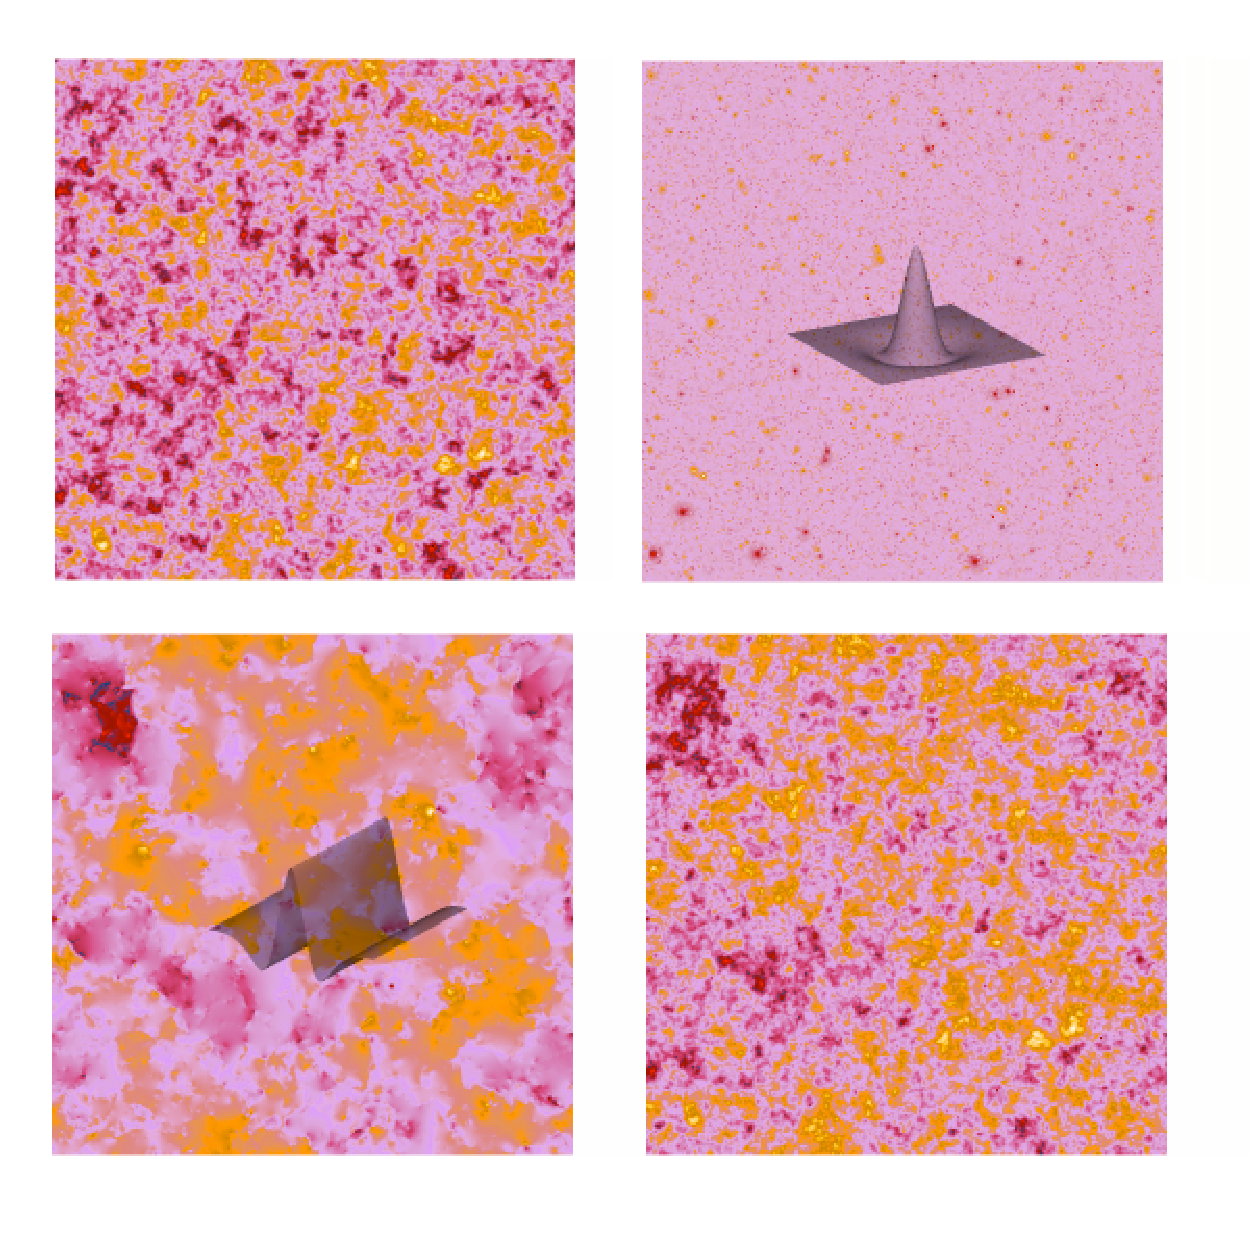
\includegraphics[width=13cm,height=13cm]{fig_cmbcssz.pdf}
\caption{Top, primary Cosmic Microwave Background anisotropies (left) and kinetic Sunyaev-Zel'dovich fluctuations (right). 
Bottom, cosmic string simulated map (left) and simulated observation containing the previous three components (right). 
The wavelet function is overplotted on the Sunyaev-Zel'dovich map and the curvelet function is overplotted on cosmic string map.}
\label{fig_cmb}
\end{figure}

In order to illustrate this, we show in Fig.~\ref{fig_cmb} a set of simulated maps. Primary CMB, kinetic SZ and cosmic string 
maps are shown respectively in Fig.~\ref{fig_cmb} top left, top right and bottom left. The ``simulated observed map", containing 
the three previous components, is displayed in Fig.~\ref{fig_cmb} bottom right. The primary CMB anisotropies dominate all the 
signals except at very high multipoles (very small angular scales). The wavelet function is overplotted on the kinetic Sunyaev-Zel'dovich 
map and the curvelet function is overplotted on cosmic string map.


CMB data are different from other astronomical data sets in the sense that they are not sparse (typical sparse data are stars or/and 
galaxies on top of a smooth background). After a component separation processing (see chapter~\ref{ch_mrs_ica}), the CMB data are not 
completely free of contaminations. Point sources still need to be detected and removed. Once we believe the data are clean enough, 
we want to check if the distribution of CMB temperature fluctuations is Gaussian by using robust statistical Gaussianity tests. 
\index{SZ effect}
\index{cosmic strings}
\index{CMB}

\section{Point Sources on a Gaussian Background}
\index{detection!point sources}
\index{wavelet!mexican hat}
\index{detection!matched filter}

Several methods have been proposed in the last years for point source detection in the CMB such as the the Mexican Hat wavelet \citep{gauss:cayon00,gauss:cayon01}, 
the pseudo-filter \citep{gauss:sanz01}, or the biparametric scale-adaptive filter \citep{gauss:sanz05}. A simple and robust technique, which maximizes 
the signal-to-noise ratio is the Matched Filter \citep{gauss:vio02}. Assuming an isotropic point spread function (PSF) with known power sprectum $\tau(q)$ 
and the CMB with power spectrum $P(q)$, the Matched Filter is \citep{gauss:vio02}:
\begin{equation} 
\label{eqn_mf}
\widehat{\psi}_{MF}(q) = \frac{1}{2 \pi \alpha}~ \frac{\tau(q)}{P(q)},\qquad \alpha \equiv \int_0^{+\infty}q \frac{\tau^2}{P} ~dq
\end{equation}
with minimum variance
\begin{equation} 
\sigma^2 = \frac{1}{2 \pi \alpha}
\end{equation}

\newpage
If the PSF is unknown (or space-variant), the Mexican Hat wavelet may be a good alternative. It consists of convolving the data 
with the wavelet function $\psi_{a,b} (x) =  \psi(\frac{x-b}{a})$, where $\psi(x)= \frac{1}{\sqrt{2\pi}}(1 - x^2) e^{- x^2/2}$. 
$a$ is the scale parameter and $b$ the position parameter. A fast implementation is obtained by using the Fourier transform to 
perform the convolution products ($\widehat{\psi}_{a}(q) = \frac{2}{\sqrt{\pi}} {(q a )}^2 e^{- \frac{1}{2}{(q a)}^2}$) \citep{gauss:sanz05}.




\section{Detecting Faint Non-Gaussian Signals Superposed on a Gaussian Signal}
\label{sec:Theory}
The superposition of a non-Gaussian signal with a Gaussian signal can be modeled as $Y = N + G$, where $Y$ is the observed image, 
$N$ is the non-Gaussian component and $G$ is the Gaussian component. We are interested in using transform coefficients to test 
whether $N \equiv 0$ or not.  

\subsection{Hypothesis Testing and Likelihood Ratio Test (LRT).}  
\label{subsec:LRT}
\index{statistic!LRT}

Transform coefficients of various kinds [Fourier, wavelet, curvelet, etc.] have been used for detecting non-Gaussian behavior 
in numerous studies. Let $X_1, X_2, \ldots, X_n$ be the transform coefficients of $Y$; we model these as  
\begin{equation}    
\label{EqAlt}
X_i = \sqrt{1 - \lam} \cdot  z_i + \sqrt{\lam} \cdot w_i,  \qquad 0< \lam < 1
\end{equation}
where $\lam >0$ is a parameter, $z_i \stackrel{iid}{\sim} N(0,1)$ are the transform coefficients of the Gaussian component $G$, 
$w_i \stackrel{iid}{\sim} W$ are the transform coefficients of the non-Gaussian component $N$, and $W$ is some unknown symmetrical 
distribution. Here without loss of generality, we assume the standard deviation for both $z_i$ and $w_i$ are $1$. 

Phrased in statistical terms, the problem of detecting the existence of a non-Gaussian component is equivalent to discriminating between the hypotheses:  
\begin{eqnarray}
\label{EqHypo2}
&H_0: \;\;\;   X_i = z_i  \label{EqHypo1}   \\
&H_1:   X_i = \sqrt{1 - \lam } \cdot z_i  + \sqrt{\lam} \cdot  w_i,   \qquad 0 < \lam < 1  
\end{eqnarray}
and $N \equiv 0$ is equivalent to $\lam \equiv 0$. We call $H_0$ the {\it null hypothesis $H_0$}, and $H_1$ the {\it alternative hypothesis}. 

% \begin{figure}
% \centering
% \includegraphics[height = 3 in]{PDF/CSDetectRegion.pdf}
% \caption{Detectable regions  in the $\alpha-r$ plane.  With $(\alpha,r)$ in the white region on the top or the undetectable region, all methods completely fail for detection. With $(\alpha,r)$ in the white region on the bottom,  both excess kurtosis and Max/HC are able to detect reliably.      While in the blue region to the left,  Max/HC is able to detect reliably, but excess kurtosis completely fails, and in the yellow region to the right, excess kurtosis is able to detect reliably, but Max/HC  completely fail.     }
% \label{Figure:Detect}
% \end{figure}

\begin{figure}[htb]
\centerline{
\hbox{
\includegraphics[width=12cm]{CSDetectRegion.pdf}%,height=12cm
% \psfig{figure=,bbllx=1.5cm,bblly=8.cm,bburx=19.5cm,bbury=23cm,height=6cm,width=7.5cm,clip=}
 }}
\caption{Detection Boundary in the $\alpha-r$ plane. The solid curve is the detection boundary of LRT, above which is not possible to detect, 
and below which it is possible to reliably detect, the dotted line segment and solid line segment together is the detection boundary for Kurtosis, 
the dotted curve and the solid curve together is the detection boundary of Max/HC. Right panel: detectable regions for Kurtosis, Max/HC.}
\label{Figure:Detect}
\end{figure}

When both $W$ and $\lam$ are known, then the optimal test for Problem (\ref{EqHypo1}) - (\ref{EqHypo2}) is simply 
the Neyman-Pearson Likelihood ratio test (LRT), \cite[Page 74 ]{Lehmann}. The size of $\lam = \lam_n$  for which 
reliable discrimination between $H_0$ and $H_1$ is possible can be derived using asymptotics. If we assume that 
the tail probability of $W$ decays algebraically, 
\begin{equation} \label{EqDefineAlg}
\lim_{x \goto \infty}   x^{\alpha}  P\{|W| > x\}  = C_{\alpha},  \qquad \mbox{$C_{\alpha}$ is a constant}
\end{equation}
(we say $W$ has a power-law tail), and we calibrate $\lam$ to decay with $n$, so that increasing amounts of data are offset by increasingly hard challenges: 
\begin{equation}   \label{EqDefineLam}
\lam = \lam_n  = n^{-r}  
\end{equation}
then there is a {\it threshold effect} for the detection problem (\ref{EqHypo1}) - (\ref{EqHypo2}). In fact, define:\\
\begin{equation} \label{EqDetectBoundary}
\rho^*_1(\alpha) = 
\left\{ \begin{array}{ll}
2/\alpha, &\   \  \alpha \leq 8 \\
1/4, &\     \       \alpha > 8
\end{array}
\right.
\end{equation}
then as $n \goto \infty$, LRT is able to reliably detect for large $n$ when $r < \rho^*_1(\alpha)$, and is unable to detect 
when $r > \rho^*_1(\alpha)$; this is proved in \citep{DJ04b}. Since LRT is optimal, it is not possible for any statistic to 
reliably detect when $r > \rho^*_1(\alpha)$. We call the curve $r = \rho^*_1(\alpha)$ in the $\alpha$-$r$ plane the 
{\it detection boundary}; see Figure \ref{Figure:Detect}.\\

In fact, when $r < 1/4$, asymptotically LRT is able to reliably detect whenever $W$ has a finite $8$-th moment, even without 
the assumption that $W$ has a power-law tail. Of course, the case that $W$ has an infinite $8$-th moment is more complicated, 
but if $W$ has a power-law tail, then LRT is also able to reliably detect if $r < 2/\alpha$. 

% One component of the above result is that, by assuming  $W$ has an 
% $\alpha$-algebraic tail 
% with $\alpha > 8$, then when $r < \frac{1}{4}$,  LRT is 
% able to reliably detect;  
% and when $r > \frac{1}{4}$, no statistic is able to detect.  
% It is interesting to notice here that, this part of the conclusion will still hold 
% when  
% the condition of requiring $W$ to have an algebraic tail is largely relaxed:  in 
% fact,  the same conclusion still holds if we only require $E[W^8] < \infty$.  It is 
% interesting to notice here that,  when $W$ has an $\alpha$-algebraic tail, 
% $E[W^8] < \infty$ if and only if $\alpha > 8$.

Despite its optimality, LRT is not a practical procedure. To apply LRT, one needs to specify the value of $\lam$ and 
the distribution of $W$, which seems unlikely to be available. We need non-parametric detectors, which can be implemented 
without any knowledge of $\lam$ or $W$, and depend on $X_i$'s only. In the next section, we are going to introduce three 
non-parametric detectors: excess kurtosis, Max and Higher Criticism (HC).   

\section{Kurtosis, HC from Wavelet and Curvelet Coefficients}
 
\subsection{Kurtosis}
\index{statistic!Kurtosis}
\index{Kurtosis}

For a statistic $T_n$, the $p$-value is the probability of seeing equally extreme results under the null hypothesis:
\[
p = P_{H_0} \{ T_n  \geq t_n(X_1,X_2, \ldots,X_n) \}
\] 
here $P_{H_0}$ refers to probability under $H_0$, and $t_n(X_1,X_2, \ldots,X_n)$ is the observed value of statistic $T_n$. 
Notice that the smaller the $p$-value, the stronger the evidence against the null hypothesis. A natural decision rule based 
on $p$-values rejects the null when $p < \alpha$ for some selected level $\alpha$, and a convenient choice is  $\alpha = 5\%$. 
When the null hypothesis is indeed true, the $p$-values for any statistic are distributed as uniform $U(0,1)$. This implies 
that the $p$-values provide a common scale for comparing different statistics. 

We now introduce two statistics for comparison. 

{\bf Excess Kurtosis ($\kappa_n$)}. Excess kurtosis is a widely used statistic, based on the $4$-th moment. 
For any (symmetrical) random variable $X$, the kurtosis is:
\[
\kappa(X) = \frac{EX^4}{(EX^2)^2} -3
\]
The kurtosis measures a kind of departure of $X$ from  Gaussianity, as $\kappa(z) =  0$.
Empirically, given $n$ realizations of $X$, the excess kurtosis statistic is defined as: 
\begin{equation}  \label{EqDefineK}
\kappa_n(X_1, X_2,\ldots,X_n)  = \sqrt{\frac{n}{24}} \biggl[ \frac{\frac{1}{n}\sum_i  X_i^4}{(\frac{1}{n}  \sum_i X_i^2)^2}  - 3  \biggr]
\end{equation} 
When the null is true, the excess kurtosis statistic is asymptotically normal:
\[
\kappa_n(X_1, X_2,\ldots,X_n)  \rightarrow_{w}  N(0,1), \qquad n \goto \infty
\]
thus for large $n$, the $p$-value of the excess kurtosis is approximately:
\[
\tilde{p} = \bar{\Phi}^{-1} (\kappa_n(X_1, X_2,\ldots,X_n))
\]
where $\bar{\Phi}(\cdot)$ is the survival function (upper tail probability) of $N(0,1)$. 

It is proved in \citep{DJ04b} that the excess kurtosis is asymptotically optimal for the hypothesis testing of \eqref{EqHypo1} - \eqref{EqHypo2} if 
\[
E [W^8] < \infty
\]
However, when $E[W^8] = \infty$, even though kurtosis is well-defined ($E[W^4] < \infty$), there are situations in which LRT 
is able to reliably detect but excess kurtosis completely fails. In fact, by assuming \eqref{EqDefineAlg} - \eqref{EqDefineLam} 
with an $\alpha < 8$, if $(\alpha,r)$ falls into the blue region of Figure~\ref{Figure:Detect}, then LRT is able to reliably detect, 
however, excess kurtosis completely fails. This shows that in such cases, excess kurtosis is not optimal; see \citep{DJ04b}. 

\subsection{Max}
\index{statistic!max}
\index{max}
The largest (absolute) observation is a classical and frequently-used non-parametric statistic:
\[
M_n =  \mmax(|X_1|,|X_2|,\ldots, |X_n|)
\] 
under the null hypothesis, 
\[
M_n  \approx \sqrt{2 \log n}
\]
and moreover, by normalizing $M_n$ with constants $c_n$ and $d_n$, the resulting statistic 
converges to the Gumbel distribution $E_v$, whose cdf is $e^{-e^{-x}}$:
\[
\frac{M_n - c_n}{d_n}  \rightarrow_{w}    E_v
\]
where approximately
\[
d_n = \frac{\sqrt{6} S_n}{\pi}, \qquad  c_n = \bar{X} - 0.5772 d_n 
\]
here $\bar{X}$ and $S_n$ are the sample mean and sample standard deviation of $\{X_i\}_{i=1}^n$ respectively. 
Thus a good approximation of the $p$-value for $M_n$ is:
\[
\tilde{p} =  \mathrm{exp}(-\mathrm{exp}(-\frac{M_n - c_n}{d_n}))
\]
We have tried the above experiment for $n = 244^2$, and found that taking $c_n = 4.2627$, $d_n = 0.2125$ gives a good approximation.  

Assuming \eqref{EqDefineAlg} - \eqref{EqDefineLam} and $\alpha < 8$, or $\lam = n^{-r}$ and that $W$ has a power-law tail 
with $\alpha < 8$, it is proved in \citep{DJ04b} that Max is optimal for hypothesis testing \eqref{EqHypo1} - \eqref{EqHypo2}. 
Recall if we further assume $\frac{1}{4} < r < \frac{2}{\alpha}$, then asymptotically, excess kurtosis completely fails; 
however, Max is able to reliably detect and is competitive to LRT. 

On the other hand, recall that excess kurtosis is optimal for the case $\alpha > 8$. In comparison, in this case, 
Max is not optimal. In fact, if we further assume $ \frac{2}{\alpha} < r < \frac{1}{4}$, then  excess kurtosis 
is able to reliably detect, but Max will completely fail. 

In Figure \ref{Figure:Detect}, we compared the detectable regions of the excess kurtosis and Max in the $\alpha$-$r$ plane. 

\subsection{Higher Criticism}
\label{sec:HC}
\index{statistic!Higher Criticism}
\index{Higher Criticism}

The Higher Criticism statistic (HC), was proposed in \citep{gauss:lin02}. To define HC first we convert the individual $X_i$'s 
into $p$-values for individual $z$-tests. Let $p_i = P\{ N(0,1) > X_i \}$ be the $i^{th}$ $p$-value, and let $p_{(i)}$ denote 
the $p$-values {\it sorted in increasing order}; the Higher Criticism statistic is defined as:
\[
       HC_{n}^* =  \max_{i}
         \biggl| \sqrt{n} [i/n  - p_{(i)}]/ \sqrt{p_{(i)} (1-p_{(i)})} \biggr|
\]
or in a modified form:
\[
HC_n^+  = \max_{\{i:  \; 1/n  \leq  p_{(i)} \leq  1 - 1/n \}}
         \biggl|   \sqrt{n} [i/n  - p_{(i)}]/ \sqrt{p_{(i)} (1-p_{(i)})}  \biggr|
\]
we let $HC_n$ refer either to $HC_n^*$ or $HC_n^+$ whenever there is no confusion. The above definition is slightly 
different from \citep{gauss:lin02}, but the ideas are essentially the same.

With an appropriate normalization sequence:
\[
a_n = \sqrt{2 \log \log n}, \qquad b_n = 2 \log \log n + 0.5 \log \log \log n - 0.5 \log (4 \pi)
\]
the distribution of $HC_n$ converges to  the Gumbel distribution $E_v^4$, whose cdf is $\mathrm{exp}(-4\mathrm{exp}(-x))$, \citep{Shorack}:
\[
a_n  HC_n - b_n  \rightarrow_w  E_v^4
\]
so the $p$-values of $HC_n$ are approximately:
\begin{equation}  
\label{EqHCP}
\mathrm{exp}(-4\mathrm{exp}( - [a_n HC_n - b_n]))
\end{equation}
For moderately large $n$, in general, the approximation in \eqref{EqHCP} is accurate for the $HC_n^+$, but not for $HC_n^*$.   

A brief remark comparing Max and HC. Max only takes into account the few largest observations, HC takes into account those outliers, 
but also moderate large observations. As a result, in general HC is better than Max, especially when we have unusually many moderately 
large observations. However, when the actual evidence lies in the middle of the distribution both HC and Max will be very weak.

% \section{The Genus and the Multiscale Genus}

\section{Experiments}

\begin{figure}[htb]
\vbox{
\centerline{
\hbox{
 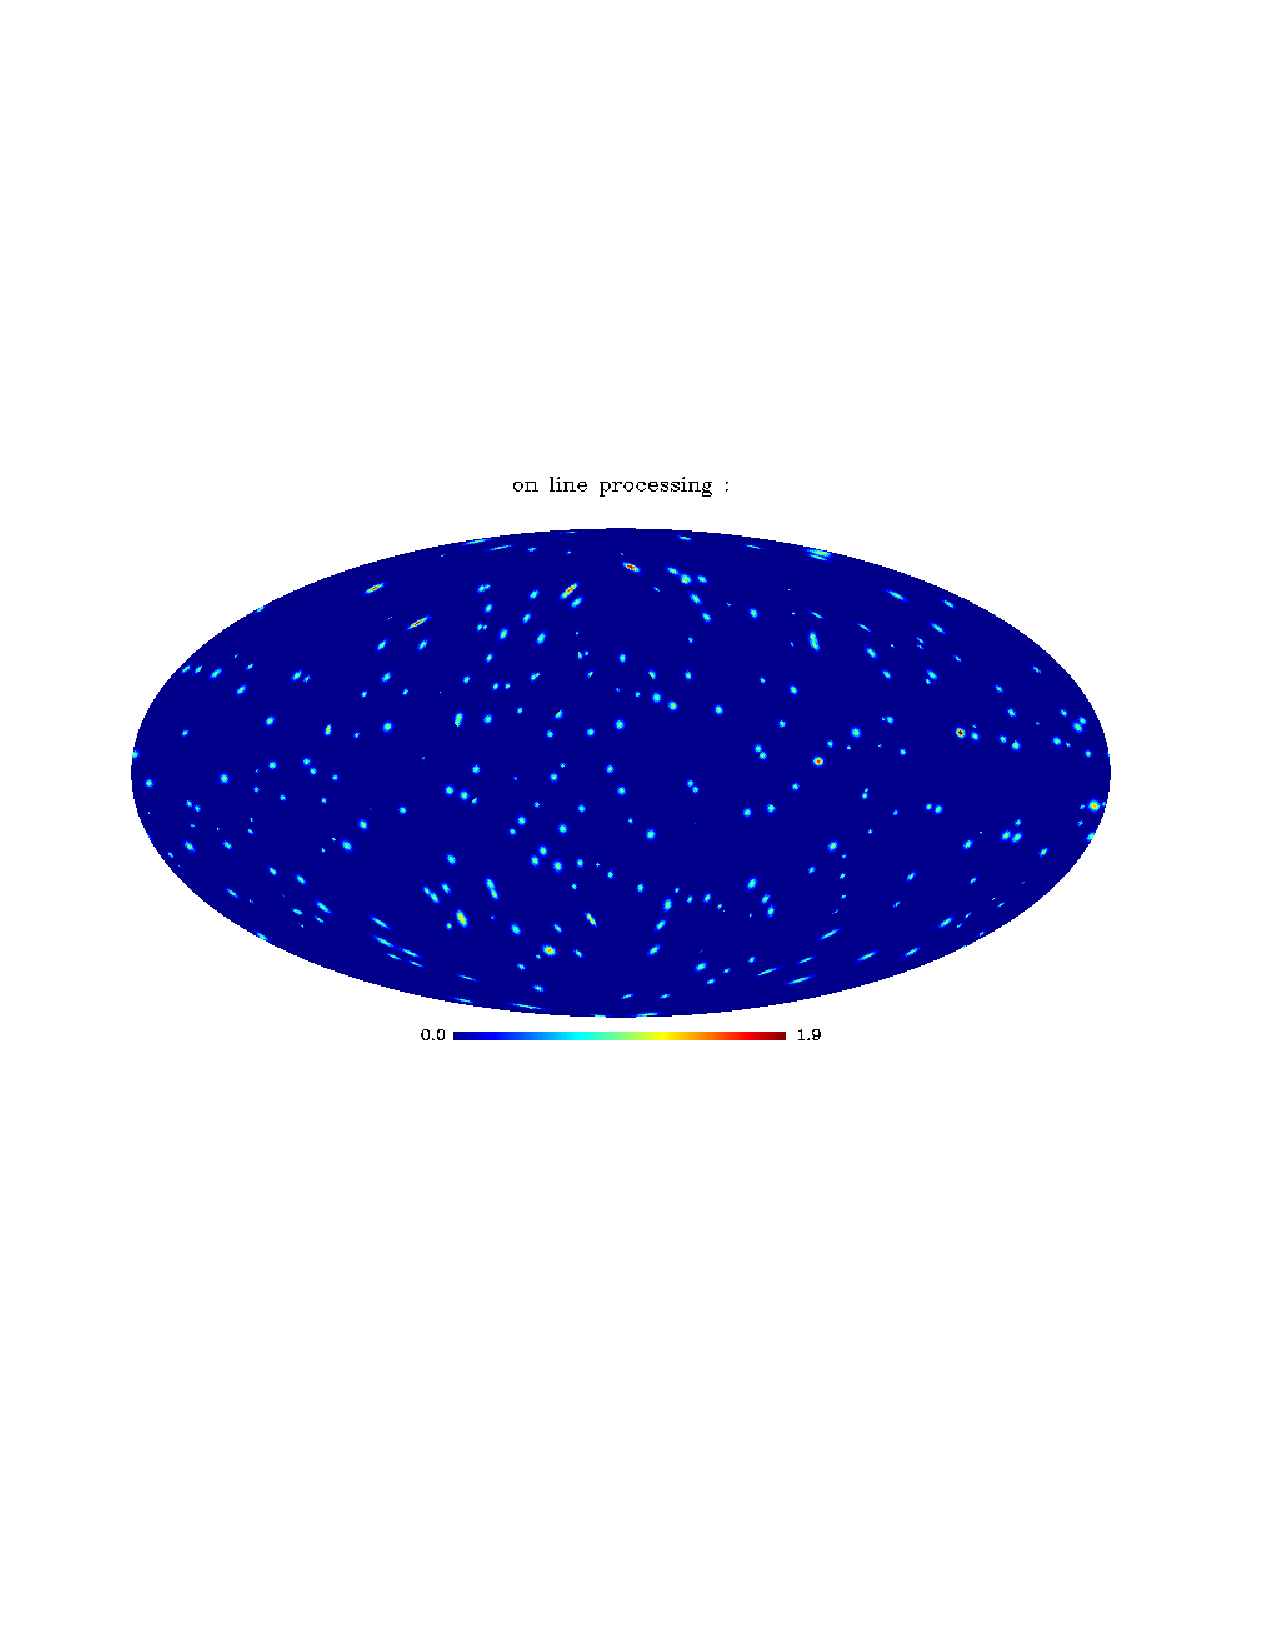
\includegraphics[trim= 2cm 8cm 2cm 8cm,width=7.9cm]{fig_sphere_gaussian.pdf}%[width=8.5cm,height=4.5cm]
 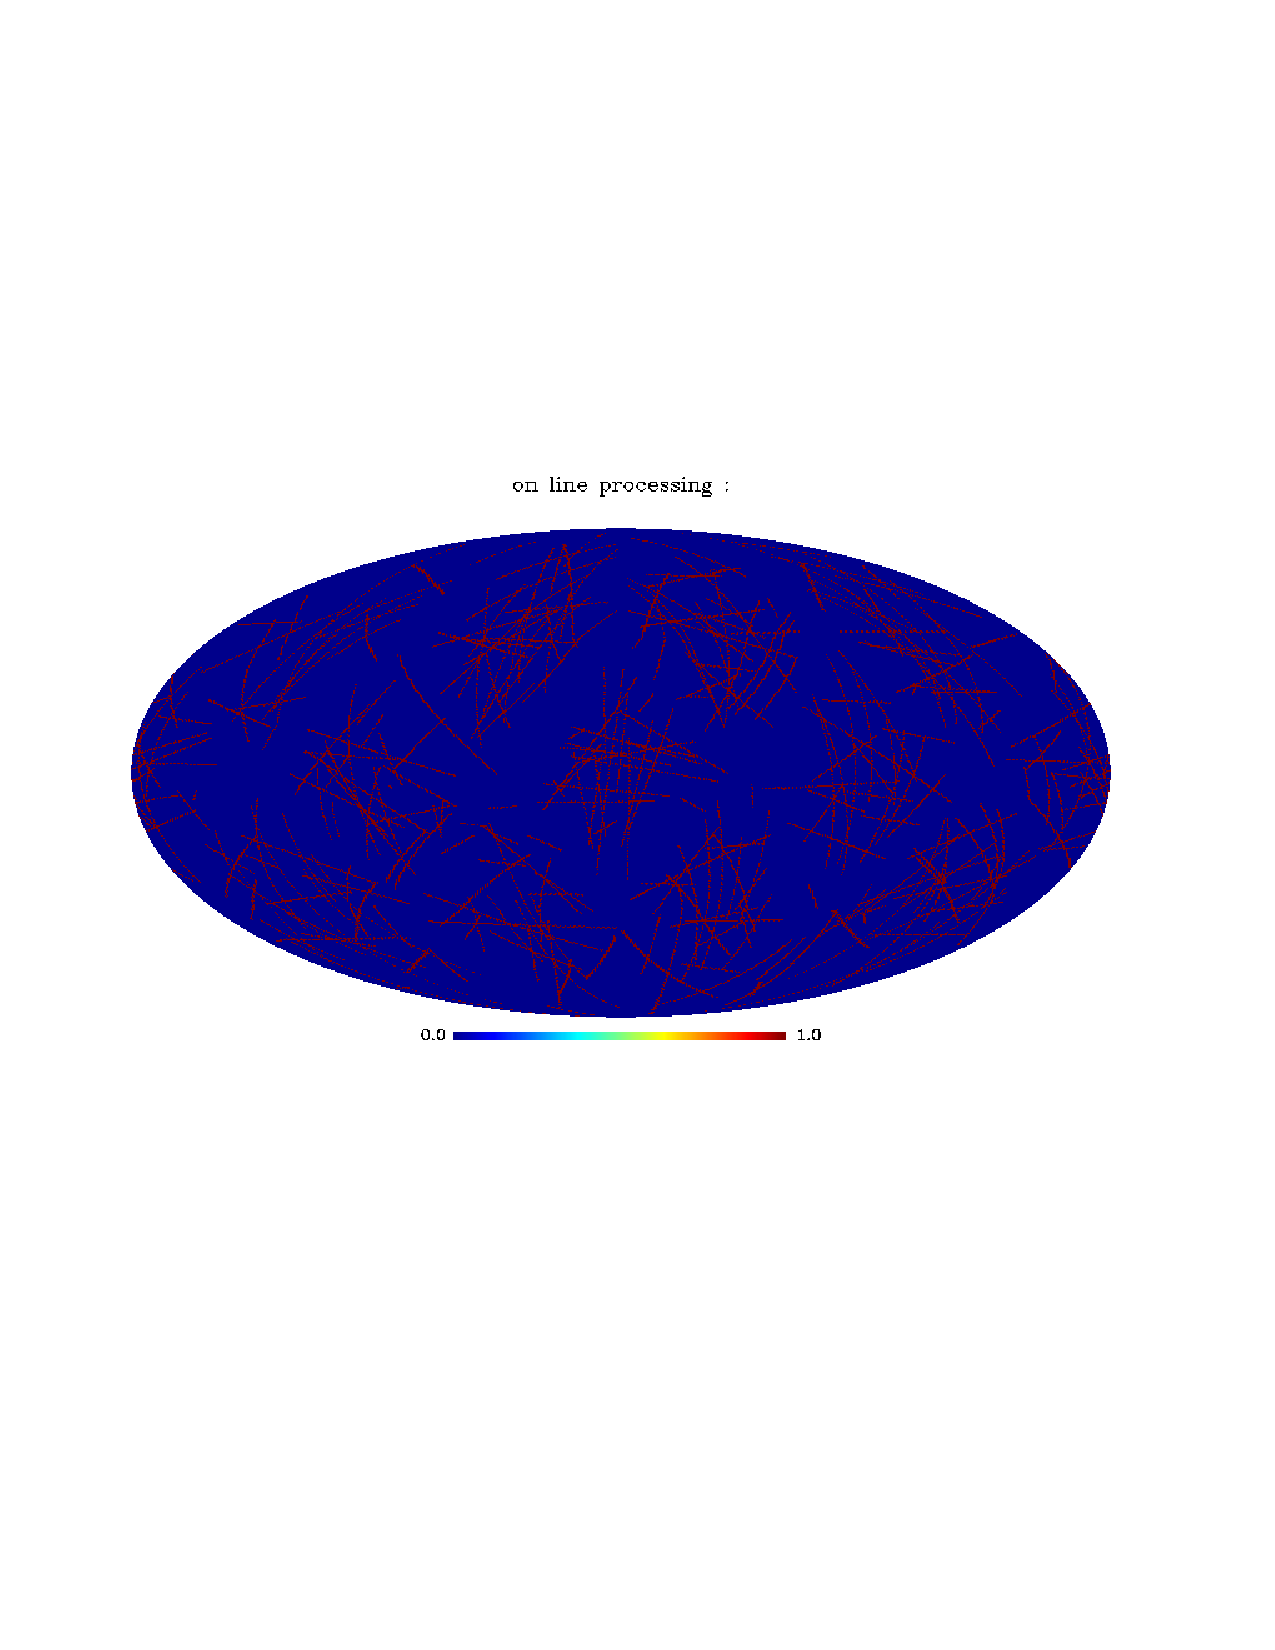
\includegraphics[trim= 2cm 8cm 2cm 8cm,width=7.9cm]{fig_sphere_line.pdf}
}}
 \centerline{
 \hbox{
 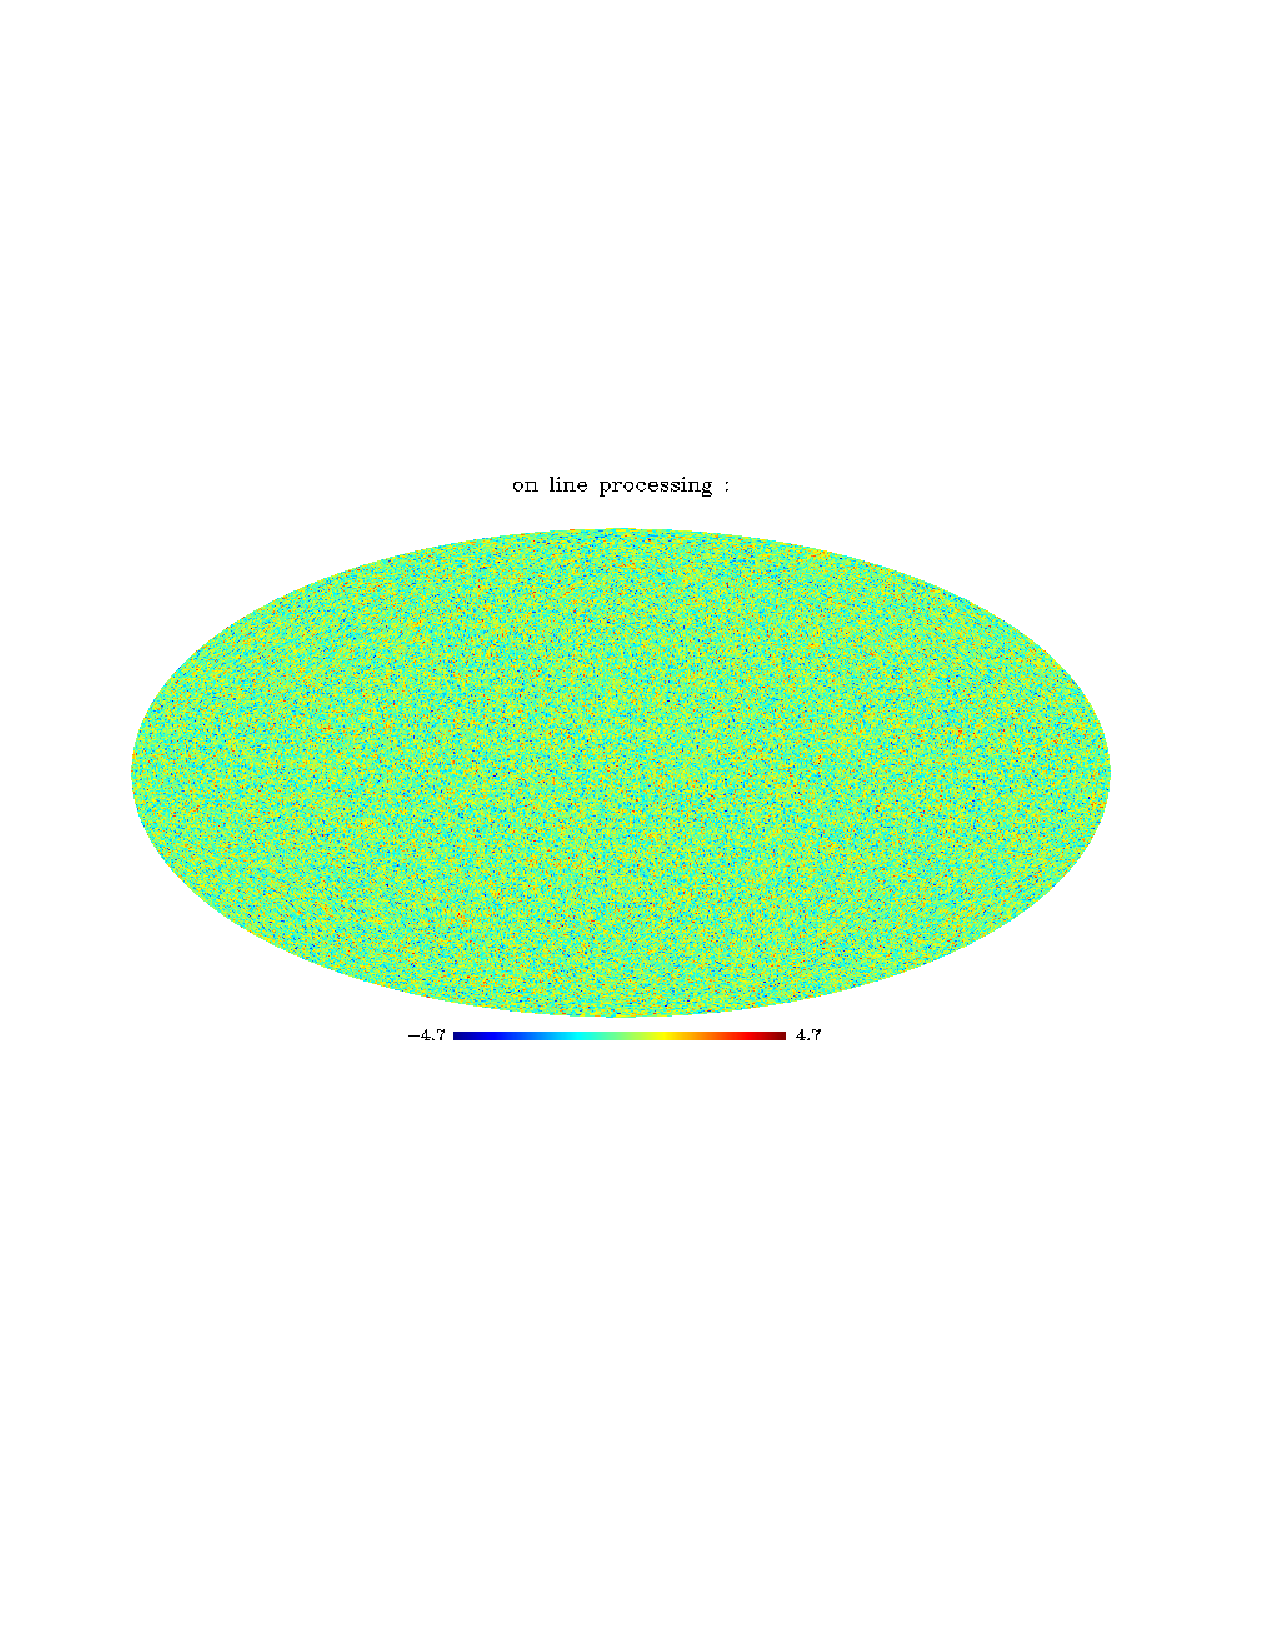
\includegraphics[trim= 2cm 8cm 2cm 8cm,width=7.9cm]{fig_sphere_gaussian_noise_snr1.pdf}
 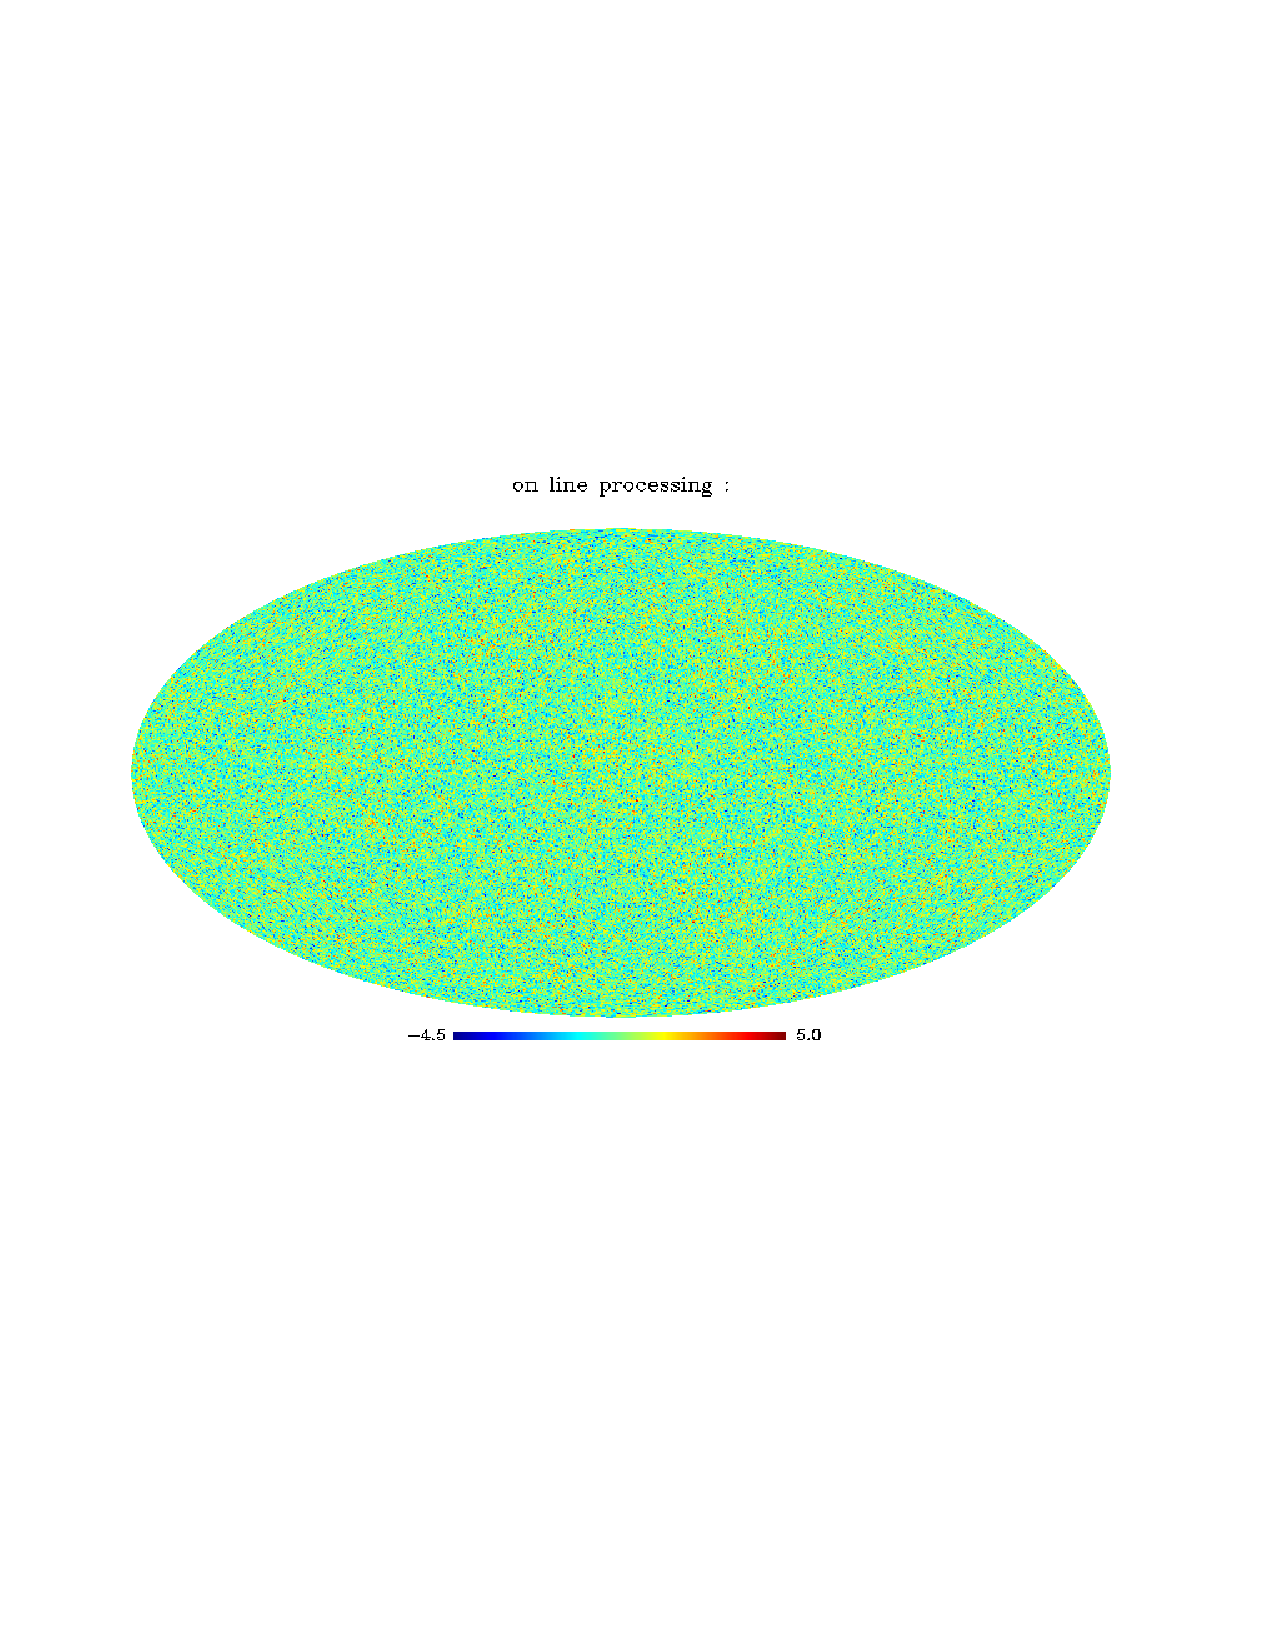
\includegraphics[trim= 2cm 8cm 2cm 8cm,width=7.9cm]{fig_sphere_line_noise_snr1.pdf}
}}}
 \caption{Top, image with Gaussians and image with lines. Bottom, same images but with an additional Gaussian noise. The SNR is equal to 1.}
\label{fig_sphere_linegauss}
\end{figure}

Fig.~\ref{fig_sphere_linegauss} shows, top left and right, two images with respectively Gaussians and lines. We have created a set 
of simulated images by adding a Gaussian white noise with different standard deviations to these two images. The Signal to Noise 
Ratio (SNR) varies between 0 and 1. For the image with lines, the SNR is defined as the pixel values along the lines divided by the 
noise standard deviation, and  for the image with Gaussians, the SNR is defined as the maximum of the Gaussians divided by the noise 
standard deviation. Fig.~\ref{fig_sphere_linegauss} shows, bottom left and right, the two noisy images with a SNR equal to 1. Hence, 
for each SNR value, we have thirty realizations of the noise, and we have calculated the kurtosis at the different scales of both the 
curvelet and the wavelet coefficients. These kurtosis values were normalized by the standard deviation of the kurtosis obtained from 
the wavelet and the curvelet transform of thirty Gaussian white noise realizations. Finally we kept for each SNR the maximum normalized 
kurtosis along the scales. Fig.~\ref{fig_wtcur_sphere_linegauss} left (resp.~right) shows the normalized kurtosis values using the wavelet 
transform (resp. the curvelet transform) for the two images (i.e. lines and Gaussians) versus the SNR. Continuous error bars correspond 
to $1\sigma$ level and dashed error bars correspond to $2\sigma$ level. We can clearly see that the detection power of the wavevet 
transform is much larger than the detection power of the curvelet transform for detecting non-Gaussianities due to isotropic features, 
while curvelets are more powerful than wavelets for detecting anisotropic features.

\begin{figure}[htb]
\centerline{
 \hbox{
% {figure=,bbllx=2.5cm,bblly=12.5cm,bburx=19.5cm,bbury=25.5cm,width=8.5cm,height=6.5cm,clip=}
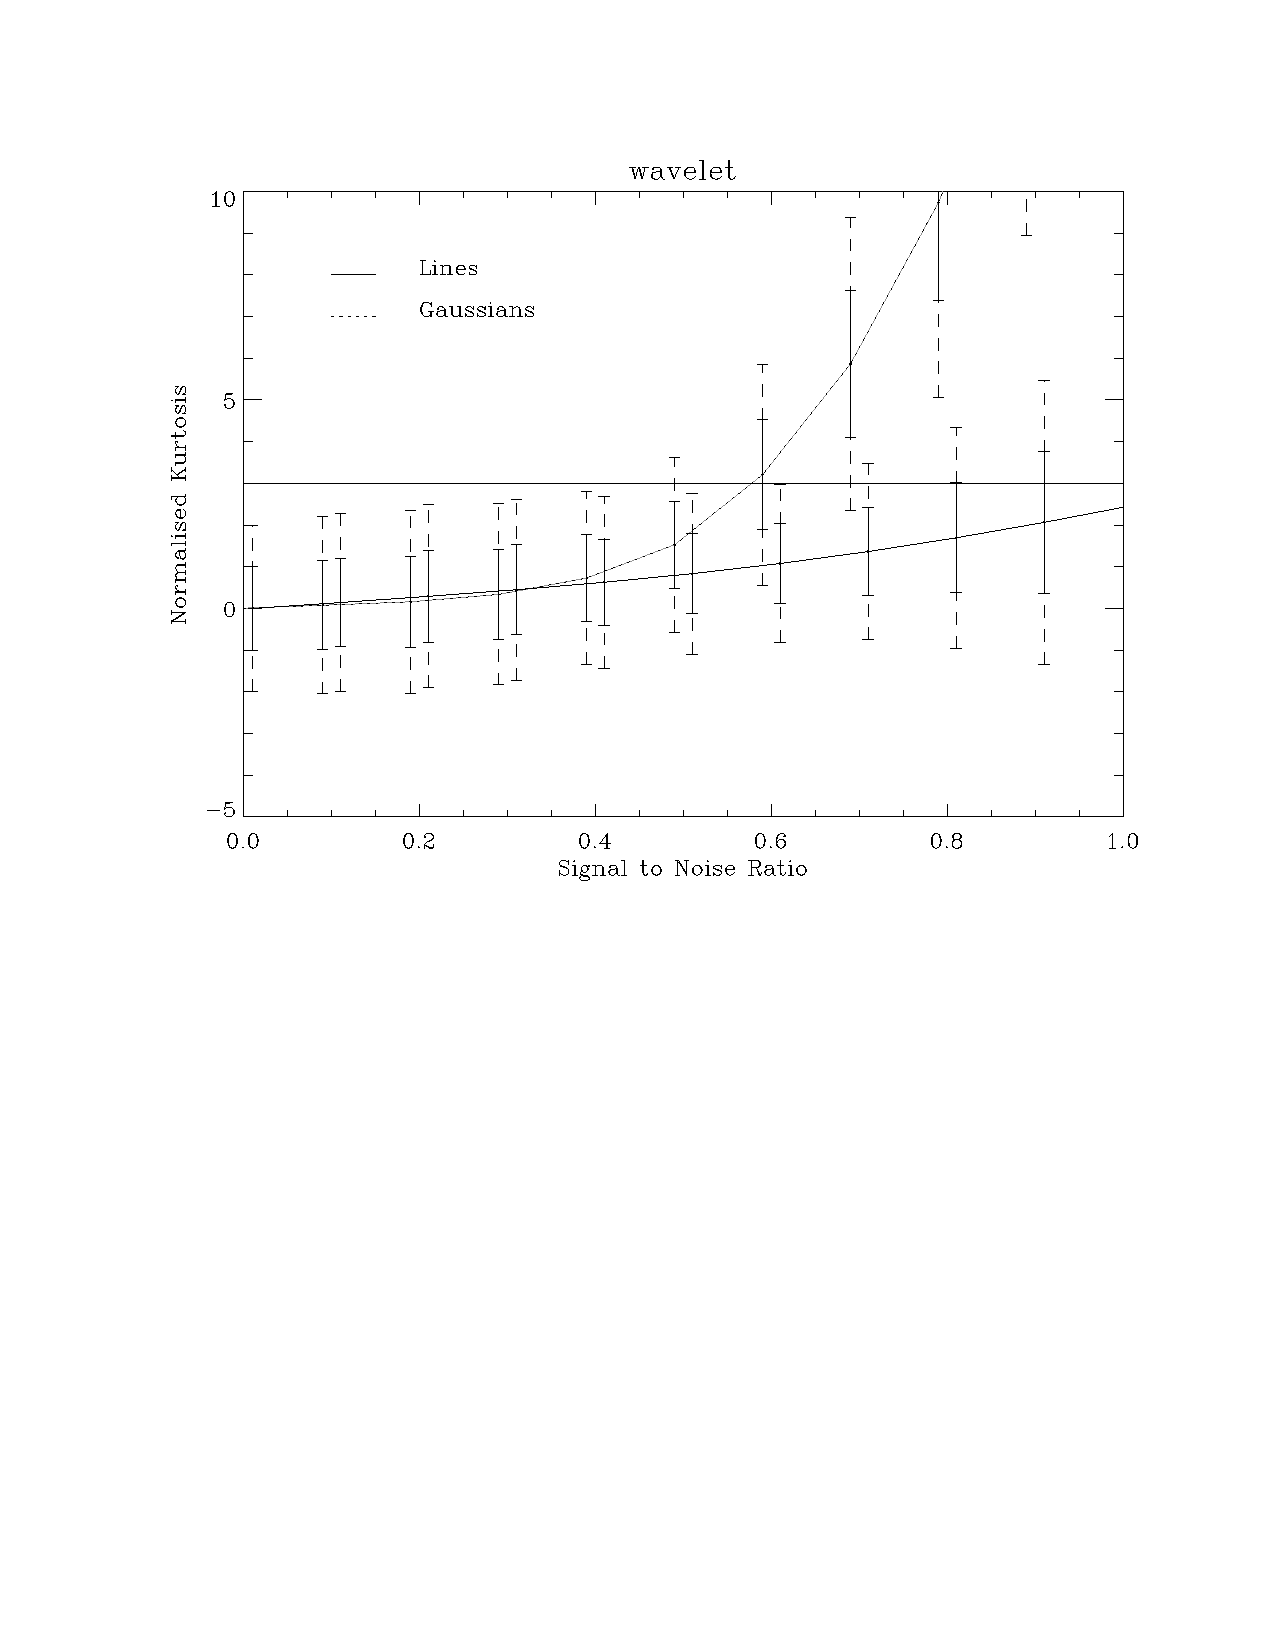
\includegraphics[trim= 2cm 13cm 2cm 3cm,width=7.9cm]{fig_sphere_wt_linedroite.pdf}%,height=6.5cm
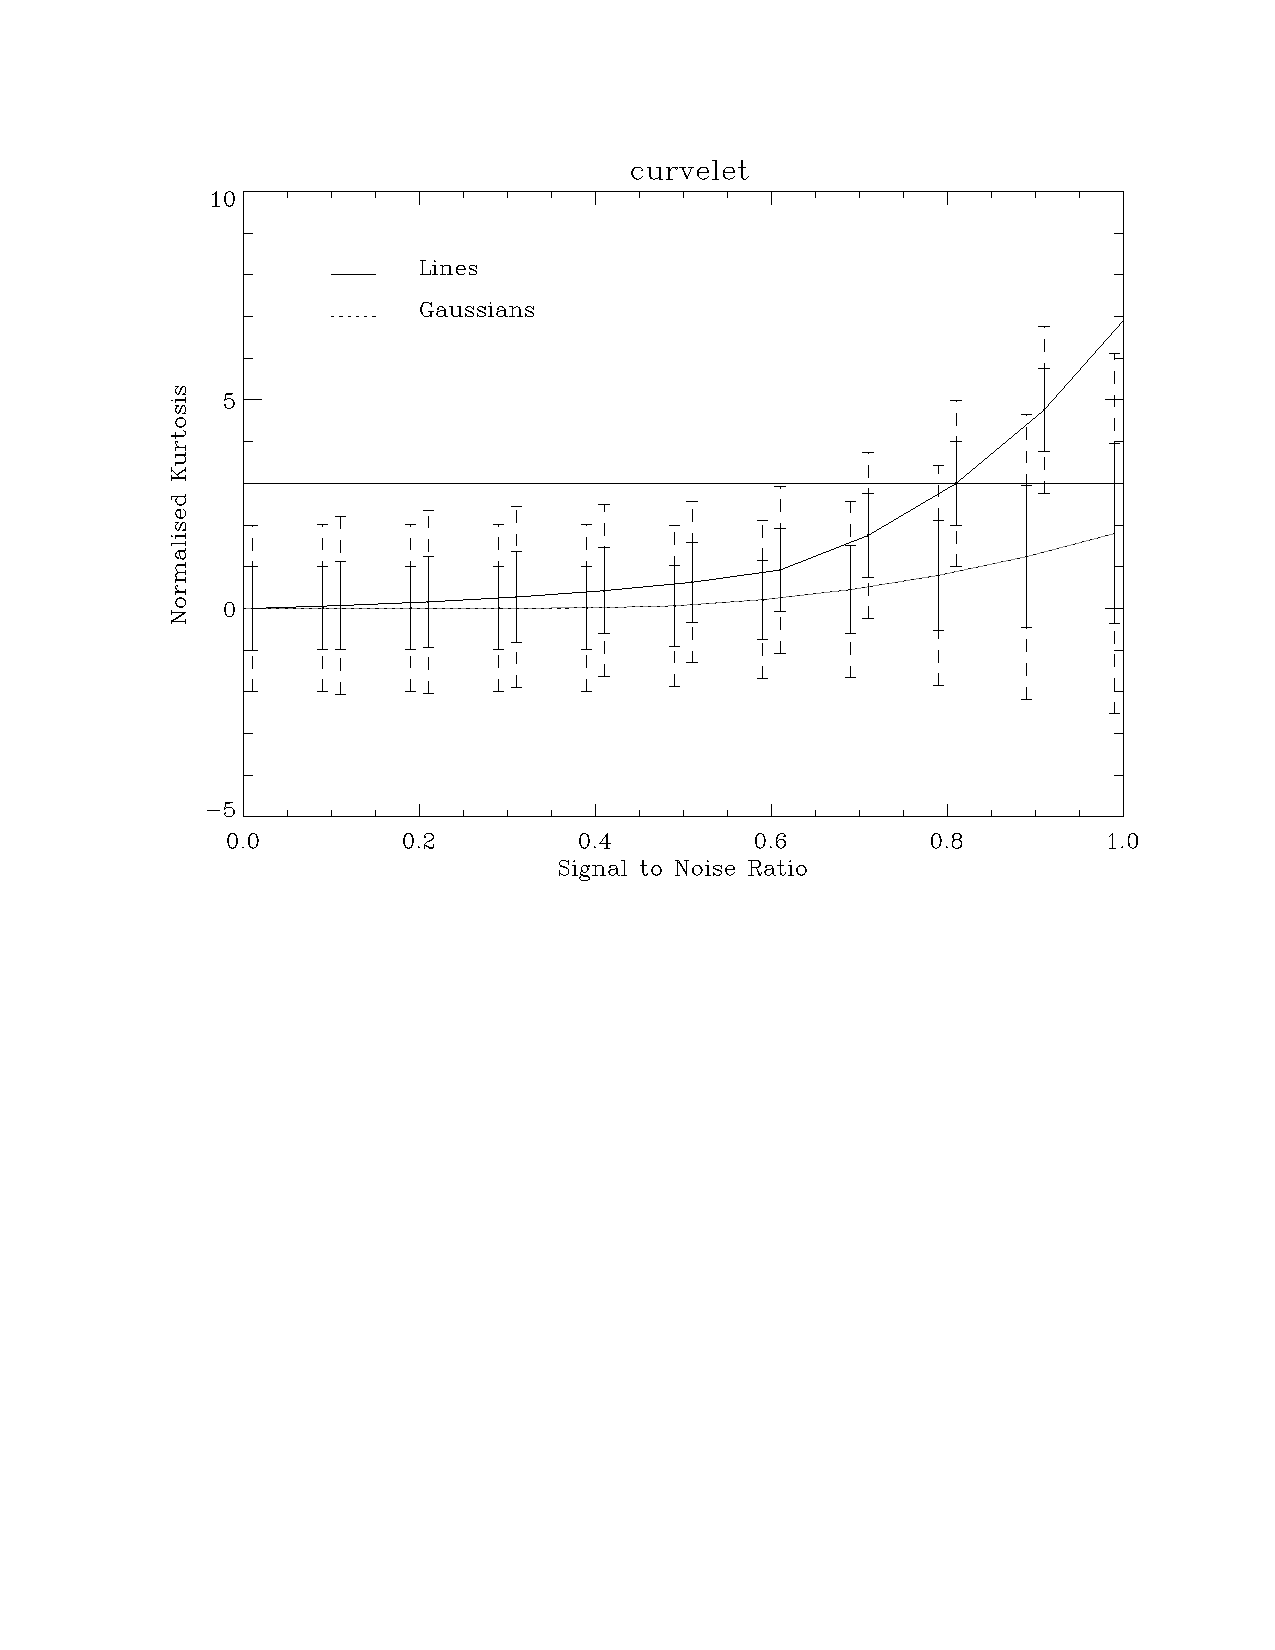
\includegraphics[trim= 2cm 13cm 2cm 3cm,width=7.9cm]{fig_sphere_cur_linedroite.pdf}
% \psfig{figure=fig_sphere_cur_linedroite.pdf,bbllx=2.5cm,bblly=12.5cm,bburx=19.5cm,bbury=25.5cm,width=8.5cm,height=6.5cm,clip=}
}}
\caption{Normalised kurtosis value versus the SNR for the wavelet coefficients (left) and the curvelet coefficients (right). 
The continuous error bars correspond to one $\sigma$ and the dashed error bars correspond to $2\sigma$.}
\label{fig_wtcur_sphere_linegauss}
\end{figure}

\section{Conclusions}
\index{wavelet!Kurtosis}
\index{wavelet!Higher Criticism}
\index{curvelet!Kurtosis}
\index{curvelet!Higher Criticism}
\index{SZ effect}
\index{cosmic strings}
\index{detection!non-Gaussianity}

The kurtosis of the wavelet coefficients is very often used in astronomy for the detection of non-Gaussianities in the CMB. It has been 
shown \citep{starck:sta03_1} that it is also possible to separate the non-Gaussian signatures associated with cosmic strings from those 
due to SZ effect by combining the excess kurtosis derived from these both the curvelet and the wavelet transform. It has been shown that 
kurtosis is asymptotically optimal in the class of weakly dependent symmetric non-Gaussian contamination with finite 8-th moments, while 
HC and MAX are asymptotically optimal in the class of weakly dependent symmetric non-Gaussian contamination with infinite 8-th moment \citep{starck:jin05}. 
Hence depending on the nature of the non-Gaussianity, a statitic is better than another one. This is a motivation for using several statistics 
rather than a single one for analysing CMB data. The case of the detection of cosmic string contaminations has been studied on simulated maps, 
and it has been shown that kurtosis outperforms clearly Max/HC \citep{starck:jin05}.  






\chapter{\projmw Programs}
\label{ch_prog_mw}
\markright{Programs}

\section{Probability in wavelet space: mw\_proba}
\index{mw\_proba}
The program 
{\em mw\_proba} computes the probability of each wavelet coefficient to be
due to signal (i.e.\ not due to noise).
{\bf 
\begin{center}
 USAGE: mw\_proba options image\_in mr\_file\_out
\end{center}}
where options are~:
\begin{itemize}
\baselineskip=0.4truecm
\itemsep=0.1truecm
\item {\bf [-t type\_of\_multiresolution\_transform]} 
\item {\bf [-m type\_of\_noise]}
\item {\bf [-g sigma]}
\item {\bf [-c gain,sigma,mean]}
\item {\bf [-n number\_of\_scales]}
\item {\bf [-S SizeBlock]} \\
\item {\bf [-N NiterSigmaClip]} \\
\item {\bf [-R RMS\_Map\_File\_Name]} \\
\end{itemize}

\subsubsection*{Examples:}
\begin{itemize}
\item mw\_prob image\_in.d MR\_File\_out.mr \\
Compute the probability of each wavelet coefficient of an image
to be due to signal (i.e. not due to noise).
\item mr\_extract -s 1 MR\_File\_out.mr  scale1.d \\
Create an image from the first scale of the multiresolution file.
\end{itemize}

\section{Entropy of an image: mw\_entrop}
\index{mw\_entrop}
The program 
{\em mw\_entrop} computes the information (entropy) and the signal information
of an image (N1-MSE approach). The two output files mr\_file1\_out and mr\_file2\_out 
are multiresolution files (``.mr'') which contain respectively 
the information and the signal information 
relative to the wavelet coefficients. The program calculates and prints to
the screen the mean entropy and signal entropy per band.
{\bf 
\begin{center}
 USAGE: mw\_entrop options image\_in  mr\_file1\_out mr\_file2\_out
\end{center}}
where options are:
\begin{itemize}
\baselineskip=0.4truecm
\itemsep=0.1truecm
\item {\bf [-t type\_of\_multiresolution\_transform]} 
\item {\bf [-m type\_of\_noise]}
\item {\bf [-g sigma]}
\item {\bf [-c gain,sigma,mean]}
\item {\bf [-n number\_of\_scales]}
\item {\bf [-S SizeBlock]} 
\item {\bf [-N NiterSigmaClip]}
\item {\bf [-R RMS\_Map\_File\_Name]}
\end{itemize}
\subsubsection*{Example:}
\begin{itemize}
\item mw\_entrop image\_in.d MR\_File1\_out.mr MR\_File2\_out.mr \\
Compute the multiscale entropy of an image
\end{itemize}

\section{Filtering}
\subsection{1D filtering: mw1d\_filter}
\index{mw1d\_filter}
The program {\em mw1d\_filter} filters a one dimensional signal using the 
multiscale entropy method (N2-MSE approach). 
{\bf 
\begin{center}
 USAGE: mw1d\_filter options signal\_in  signal\_out
\end{center}}
where options are~:
\begin{itemize}
\baselineskip=0.4truecm
\itemsep=0.1truecm
\item {\bf [-t type\_of\_multiresolution\_transform]} 
\item {\bf [-m type\_of\_noise]}
\item {\bf [-g sigma]} 
\item {\bf [-c gain,sigma,mean]}
\item {\bf [-s NSigma]} 
\item {\bf [-n number\_of\_scales]} 
\item {\bf [-e epsilon]} \\
Convergence parameter. Default is $1e^{-4}$.
\item {\bf [-i number\_of\_iterations]} \\
Maximum number of iterations. Default is 10.
\item {\bf [-G RegulParam]} \\
Regularization parameter. Default is 1.
\item {\bf [-D]} \\
The regularization parameter is a function of the SNR in the data.
Default is no.
\item {\bf [-w FilterCoefFileName]} \\
Write to  disk the filtered wavelet coefficient.
\item {\bf [-v]} \\
Verbose. Default is no.
\end{itemize}

\subsubsection*{Examples:}
\begin{itemize}
\baselineskip=0.4truecm
\itemsep=0.1truecm
\item mw1d\_filter sig\_in.fits sig\_out.d \\
filters a signal by the multiscale entropy method, assuming
Gaussian noise (its standard deviation is automatically estimated).
\item mw1d\_filter -G 2 sig\_in.fits sig\_out.fits \\
Same as before, but the regularization will be stronger, and the solution
more smooth.  
\item mw1d\_filter -G 2 -D sig\_in.fits sig\_out.fits \\
The regularization is adaptive, depending on the wavelet SNR.
\item mw\_filter -G 2 -D -s 5 sig\_in.fits sig\_out.fits \\ 
Same as before, preserving  feature in the wavelet space greater than
$5\sigma$ instead of the default $3\sigma$ value.
\end{itemize}


\subsection{2D filtering: mw\_filter}
\index{mw\_filter}
The program {\em mw\_filter} filters an image using the 
multiscale entropy method (N2-MSE approach). 
{\bf 
\begin{center}
 USAGE: mw\_filter options image\_in image\_out
\end{center}}
where options are:
\begin{itemize}
\baselineskip=0.4truecm
\itemsep=0.1truecm
\item {\bf[-T Type\_of\_Regularization]}
\begin{enumerate}
\baselineskip=0.4truecm
\itemsep=0.1truecm
\item Use a fixed user Alpha value.
\item Estimate the optimal Alpha.
\item Estimate one  Alpha value per band.
\end{enumerate}
Default is 1.
\item {\bf [-D]} \\
Wavelet coefficients with a high signal to noise ratio are not
regularized. For a lower SNR, the Alpha parameter is modified using the SNR.
Default is no regularization.
\item {\bf [-t type\_of\_multiresolution\_transform]} 
\item {\bf [-m type\_of\_noise]} \\
Noise models 1 to 9 are available.
\item {\bf [-g sigma]} 
\item {\bf [-c gain,sigma,mean]}
\item {\bf [-s NSigma]} 
\item {\bf [-S SizeBlock]} 
\item {\bf [-N NiterSigmaClip]} 
\item {\bf [-R RMS\_Map\_File\_Name]} 
\item {\bf [-n number\_of\_scales]} 
\item {\bf [-e epsilon]} \\
Convergence parameter. Default is $1e^{-4}$.
\item {\bf [-i MaxIter]} \\
Maximum number of iterations. Default is 20.
\item {\bf [-G RegulParam]} \\
Regularization parameter. Default is 1.
\item {\bf [-C]} \\
Convergence parameter. Only used when regularization type is equal to
2 or 3.
Default is $0.01$.
\item {\bf [-P]} \\
Apply the positivity constraint. If set, the solution cannot have negative 
values.
\item {\bf [-v]} \\
Verbose. Default is no.
\end{itemize}

\subsubsection*{Examples:}
\begin{itemize}
\baselineskip=0.4truecm
\itemsep=0.1truecm
\item mw\_filter image\_in.d ima\_out.d \\
Filters an image by the multiscale entropy method, assuming
Gaussian noise (its standard deviation is automatically estimated).
\item mw\_filter -G 10 -P image\_in.d ima\_out.d \\
Same as before, but the regularization will be stronger, and the solution
more smooth. Positivity constraint is imposed.
\item mw\_filter -G 10 -D image\_in.d ima\_out.d \\
The regularization is adaptive, depending on the wavelet SNR.
\item mw\_filter -T 2 image\_in.d ima\_out.d \\
The regularization parameter is automatically estimated in an iterative way.
\item mw\_filter -T 2 -G 2.5 image\_in.d ima\_out.d \\
Same as before, but the estimated parameter is multiplied by $2.5$ (the solution
becomes more smooth).
\item mw\_filter -T 3 image\_in.d ima\_out.d \\
On regularization parameter per scale is now used. All are automatically 
estimated in an iterative way.
\item mw\_filter -T 3 -D -s 5 image\_in.d ima\_out.d \\ 
Same as before, preserving also feature in the wavelet space greater than
$5\sigma$.
\end{itemize}


\subsection{2D combined filtering: mw\_comb\_filter}
\index{mw\_comb\_filter}
The program {\em mw\_comb\_filter} filters an image using the 
combined filtering method. 
{\bf 
\begin{center}
 USAGE: mw\_comb\_filter options image\_in image\_out
\end{center}}
where options are~:
\begin{itemize}
\baselineskip=0.4truecm
\itemsep=0.1truecm
\item {\bf [-t type\_of\_multiresolution\_transform]} 
\item {\bf [-O]} \\
 Filtering by an opening (erosion+dilation). \\
The structural element is a circle of size 3
\item {\bf [-M type\_of\_multiresolution\_transform]} \\
 Filtering using the MEM method (estimating automatically
 one  Alpha value per band). Default multiresolution transform is
 the \`a trous algorithm. 
\item {\bf [-D]} \\
Wavelet coefficient with a high signa to noise ratio are not
regularized. The Alpha parameter is modified using the SNR.
Default is no. Valid only when ``-d'' or ``-M'' option is set.
\item {\bf [-G RegulParam]} \\
Regularization parameter for MEM method. 
Valid only when ``-d'' or ``-M'' option is set. \\
Default is 1.
\item {\bf [-m type\_of\_noise]}
\begin{enumerate}
\baselineskip=0.4truecm
\item Gaussian noise 
\item Poisson noise 
\item Poisson noise + Gaussian noise 
\item Multiplicative noise 
\end{enumerate}
Default is Gaussian noise.
\item {\bf [-g sigma]} 
\item {\bf [-c gain,sigma,mean]}
\item {\bf [-s NSigma]} 
\item {\bf [-n number\_of\_scales]} 
\item {\bf [-d]} \\
Use default combined methods (methods are a thresholding by the 
\`a trous algorithm,
the multiscale median transform, the orthogonal wavelet transform, the haar
transform, and the multiscale entropy method. ``-d'' option is equivalent to
the set of following options together: ``-t 2 -t 4 -t 14 -t 18 -M 2''.
\item {\bf [-v]} \\
Verbose. Default is no.
\end{itemize}
\subsubsection*{Examples:}
\begin{itemize}
\item mw\_comb\_filter -d image\_in.d ima\_out.d \\
Filters an image by the combined filtered method (default option), assuming
Gaussian noise (its standard deviation is automatically estimated).
\item mw\_comb\_filter -t 2 -t 4 -t 14 -t 18 -M 2 image\_in.d ima\_out.d \\
Ditto. 
\item mw\_comb\_filter -d -O -t 1 image\_in.d ima\_out.d \\
Same as before, with in addition a filtering using the linear \`a trous
 algorithm, and the morphological operators.
\item mw\_comb\_filter -t 14 -M 14 image\_in.d ima\_out.d \\
Filtering using only two methods: thresholding the orthogonal WT, and the MEM 
method.
\item mw\_comb\_filter -t 14 -M 14 -G 2.5 image\_in.d ima\_out.d \\
Ditto, but the estimated MEM parameter is multiplied by $2.5$.
\end{itemize}

\section{Deconvolution: mw\_deconv}
 \index{ mw\_deconv}
The program {\em mw\_deconv} deconvolves  an image using the 
multiscale entropy method. 
{\bf 
\begin{center}
 USAGE: mw\_deconv options image\_in psf\_in image\_out
\end{center}}
where options are~:
\begin{itemize}
\baselineskip=0.4truecm
\itemsep=0.1truecm
\item {\bf [-t type\_of\_multiresolution\_transform]} \\
Default is 2.
\item {\bf [-H EntropyFunction]} 
\begin{enumerate}
\baselineskip=0.4truecm
\itemsep=0.1truecm
\item Entropy = $H$ = Wavelet coefficient energy.
\item Entropy = $H_n$ = Noise information (for Gaussian noise only), using 
N2-MSE approach.
\end{enumerate}
Default is 1. For Gaussian noise, default is 2.
\item {\bf [-g sigma]} 
\item {\bf [-c gain,sigma,mean]}
\item {\bf [-m type\_of\_noise]} \\
Noise models 1 to 9 are available.
\item {\bf [-n number\_of\_scales]} 
\item {\bf [-s NSigma]} 
\item {\bf [-i number\_of\_iterations]} \\
 Maximum number of iterations. Default is 500.
\item {\bf [-K]}  \\
Suppress the last scale. Default is no. 
\item {\bf [-R RMS\_Map\_File\_Name]} \\
\item {\bf [-P]} \\
Suppress the positivity constraint.

\item {\bf [-C]} \\
Convergence parameter.
Default is $1$.
\item {\bf  [-f ICF\_Fwhm]} \\
Intrinsic correlation function. \\
Fwhm = Full-width at half maximum.
\item {\bf [-I ICF\_FileName]} \\
Intrinsic correlation function file.
\item {\bf [-F First\_Guess]} \\
Input solution file.
\item {\bf [-W DataWeightingType]} 
\begin{enumerate}
\baselineskip=0.4truecm
\item no weighting 
\item soft weighting
\item hard weighting 
\end{enumerate}
Default is 3.
\item {\bf [-A RegulProtectType]}
\begin{itemize}
\baselineskip=0.4truecm
\itemsep=0.1truecm
\item{0: } no regularization (all protected) 
\item{1: } no protection from regularization 
\item{2: } soft protection 
\item{3: } hard protection 
\item{4: } soft + hard protection 
\end{itemize}
Default is 3.
\item {\bf [-G RegulParam]} \\
Regularization parameter. Default is 1.
\item {\bf [-M NSigmaObj]} \\
NSigma level for object multiresolution determination.
Default is 3. With hard weighting (-W 3), default is 1.

\item {\bf [-r residual\_file\_name]} \\
 Write the residual to disk. 
\item {\bf [-S]} \\
Do not shift automatically the maximum of the PSF at the center.
\item {\bf [-v]} \\
Verbose. Default is no.
\end{itemize}
\subsubsection*{Example:}
\begin{itemize}
\baselineskip=0.4truecm
\itemsep=0.1truecm
\item mw\_deconv image\_in.d psf ima\_out.d \\
 Deconvolve an image using default options
\item mw\_deconv -W 3 -A 0  image\_in.d psf ima\_out.d \\
Deconvolution from the multiresolution support.
\item mw\_deconv -A 3 image\_in.d psf ima\_out.d \\
Regularization with a protection of high SNR wavelet coefficients.
\item mw\_deconv -A 3 -G 2.5 image\_in.d psf ima\_out.d \\
Ditto, but increases the regularization (solution more smooth).
\item mw\_deconv -f 3 image\_in.d psf ima\_out.d \\
Impose that the solution is the result of the convolution product between
a Gaussian (full-width at half maximum equal to 3) and a hidden solution.
\end{itemize}


\section{IDL Routines}
\label{ch_mr2_idl}
%\chapterhead{IDL Routines}
\markright{IDL Routines}

\subsection{Introduction}
A set of routines has been developed in IDL. Starting IDL using
the script program {\em mre} allows the user to get the multiresolution
environment, and all routines
described in the following can be called. An online help facility 
is also available by
invoking the {\em mrh} program under IDL.

\subsection{mw1d\_filter}
Filter a 1D signal by the the multiscale entropy.
{\bf
\begin{center}
     USAGE: mw1d\_filter, Signal, Result, Opt=Opt
\end{center}}
where 
\begin{itemize}
\item {\em Signal}: input  one-dimensional IDL array.
\item {\em Result}: output one-dimensional IDL array (filtered signal).
\item {\em Opt}:  string which contains the different options 
(see the {\em mw1d\_filter} C++  program).
\end{itemize}

\subsection{mw1d\_predict}
Considering a temporal signal $S$ with $n$ measures ($S[0..n-1]$), 
 {\em mr1d\_predict} estimates (or predicts) the next values $S[n .. n+dt]$.
A multiscale transformation is first applied, followed by filtering
in the wavelet space. At each scale, a predictor is then applied,
and the predicted signal is obtained from the reconstruction of
the predicted signal. 

{\bf
\begin{center}
     USAGE: Result = MW1D\_PREDICT(Signal,wave=wave,PredWave=PredWave,
                      NPredict=NPredict, Nscale=Nscale,  OPT=OPT, NCoef=NCoef)
\end{center}}
where 
\begin{itemize}
\item {\em wave}: output 2D IDL array; filtered wavelet coefficient
\item {\em PredWave}: output 2D IDL array; Predicted wavelet coefficient
\item {\em NPredict}: number of values to predict. Default is one.
\item {\em Nscale}: number of scales used for the wavelet transform
\item {\em NCoef:} Number of coefficients used for the prediction. Default is 3.
\item {\em OPT}: string which contains the differents options accepted by the
mw1d\_filter C++ program.
\end{itemize}

\subsection{mw\_filter}
Filter  an image by the multiscale entropy. 
This routine is calling the C++ executable {mw\_filter}. The keyword 
``OPT" allows 
all options described in the section corresponding to the 
 {\em mw\_filter} program.

{\bf
\begin{center}
     USAGE: mw\_filter, Data, FilterData, opt=opt
\end{center}}
{\em Data} is an image (2D IDL array), and {\em FilterData} is the result
of the filtering.

\subsection{mw\_deconv}
Deconvolve an image by  the  multiscale entropy. This routine calls 
the C++ executable {mw\_deconv}. The keyword ``OPT" 
allows 
all options described in the section corresponding to the 
 {\em mw\_deconv} program.

{\bf
\begin{center}
     USAGE: mw\_deconv, Data, PSF, DeconvData, opt=opt
\end{center}}
\subsubsection*{Examples:} 
\begin{itemize}
\item mw\_deconv, Imag, Psf, Result \\
deconvolve an image with all default options.
\item  mw\_deconv, Imag, Psf, Result, OPT='-i 30 -e 0'  \\
same example, but impose the number of iterations to be 30.
\end{itemize}

 


\chapter*{Appendix A: The ``\`A Trous'' Wavelet Transform Algorithm}
\addcontentsline{toc}{chapter}{Appendix A: The ``\`A Trous'' Wavelet Transform Algorithm}

In a wavelet transform, a series of transformations of a signal is 
generated, providing a resolution-related set of  ``views'' of the signal.  
The properties satisfied by a wavelet transform, and in particular by the
{\it \`a trous} wavelet transform, are further discussed by Bijaoui et al. \cite{starck:bij94_1}. 
Extensive literature exists on the wavelet transform
and its applications (\cite{wave:daube88,wave:chui92,wave:ruskai92,starck:book98}). 
The discrete {\it \`a trous} algorithm is described in \cite{wave:hol89,wave:shensa92}.

We consider spectra, 
$\{c_0(k)\}$, defined as  the scalar product at 
samples $k$ of the function $f(x)$ with a scaling function $\phi(x)$
which corresponds to a low pass filter:
\begin{eqnarray}
c_0(k) = < f(x), \phi(x-k)>
\end{eqnarray}
The scaling function is chosen to satisfy the dilation equation:
\begin{eqnarray}
\frac{1}{2}\phi(\frac{x}{2}) = \sum_l h(l)\phi(x-l)
\end{eqnarray}
where $h$ is a discrete low-pass filter associated with the scaling function
$\phi$.  This means that a low-pass filtering
of the signal is, by definition, closely linked to another resolution level
of the signal.  The distance between levels increases by a factor 2 from one
scale to the next.


The smoothed data $c_j(k)$ at a given resolution $j$ and at a position
$k$  is the scalar product 

\begin{eqnarray}
c_j(k)= \frac{1}{2^j}< f(x), \phi(\frac{x-k}{2^j})>
\end{eqnarray}

This is consequently obtained by the convolution:
\begin{eqnarray}
c_j(k) = \sum_l h(l) \ \ c_{j-1} (k+2^{j-1}l)
\end{eqnarray}
The signal difference $w_j$ between two consecutive resolutions is:
\begin{eqnarray}
w_j(k) = c_{j-1}(k) - c_j(k) 
\end{eqnarray}
or:
\begin{eqnarray}
w_j(k) = \frac{1}{2^j}< f(x), \psi(\frac{x-k}{2^j})>  
\label{wj}
\end{eqnarray}
Here, the wavelet function $\psi$ is defined by:
\begin{eqnarray}
\frac{1}{2}\psi(\frac{x}{2})  = \phi(x) - \frac{1}{2}\phi(\frac{x}{2})
\end{eqnarray}

Equation~\ref{wj} defines the discrete wavelet transform, for a  
resolution level $j$.

For the scaling function, $\phi(x)$, the B-spline of degree 3 
was used in our calculations. As a filter we use 
$h = ( \frac{1}{16}, \frac{1}{4}, \frac{3}{8}, \frac{1}{4}, \frac{1}{16})$. 
See  Starck (1993)
for discussion of 
linear and other scaling functions.  Here  
we have derived a simple algorithm in order to compute the 
associated wavelet transform:
\begin{enumerate}
\item We initialize $j$ to 0 and we start with the data $c_j(k)$.
\item We increment $j$, and carry out a discrete convolution of the data
$c_{j-1}(k)$ using  the filter $h$. The distance between the central sample
and the adjacent ones is $2^{j-1}$.
\item After this smoothing, we obtain the discrete wavelet transform
from the difference $c_{j-1}(k) - c_j(k)$.
\item If $j$ is less than the number $p$ of resolutions we want to
compute, then we go to step 2.
\item The set ${\cal W} = \{ w_1, ..., w_p, c_p \}$ represents the
wavelet transform of the data.
\end{enumerate}

A series expansion of the original signal, $c_0$, 
in terms of
the wavelet coefficients is now given as follows. 
The final smoothed array $c_{p}(x)$ is added to all the differences $w_j$:
\begin{eqnarray}
c_0(k) = c_{p} + \sum_{j=1}^{p} w_j(k)
\label{eqn_rec}
\end{eqnarray}
 This equation provides a reconstruction formula for the original signal. At each scale $j$, we obtain a set $\{w_j\}$ which 
we call a wavelet scale.  The  wavelet scale 
has the same number of samples as the signal. 

\chapter*{Appendix B: Noise Modeling the Wavelet Space}
\addcontentsline{toc}{chapter}{Appendix B: Noise Modeling the Wavelet Space}
 

\subsection*{Gaussian noise}
\index{noise}
We have the probability density
\begin{eqnarray}
p(w_j(x,y)) = \frac{1}{\sqrt{2\pi} \sigma_j} e^{{-w_j(x,y)^2}/2\sigma^2_j} 
\end{eqnarray}

So we need to estimate, in the case of Gaussian noise models,
 the noise standard deviation at each scale.  These standard deviations can 
be determined analytically in the case of some transforms, including the 
\`a trous transform, but the calculations can become complicated.  

The appropriate value of $\sigma_j$ 
in the succession of wavelet planes is assessed 
from the standard deviation of the noise $\sigma_I$ in the original image
$I$, 
and from study of the noise in the wavelet space.  This study consists of 
simulating an image containing Gaussian noise with a standard deviation 
equal to 1, and taking the wavelet transform of this image.  Then we
compute the standard deviation $\sigma^e_j$ at each scale.  We get a curve 
$\sigma^e_j$ as a function of $j$, giving the behavior of the noise in the 
wavelet space.
(Note that if we had used an orthogonal wavelet transform, this curve would
\index{wavelet transform}
be linear.)  Due to the properties of the wavelet transform, we have 
$ \sigma_j = \sigma_I \sigma^e_j $.
The standard deviation of the noise at a scale $j$ of the image is equal to
the standard deviation of the noise of the image multiplied by the 
standard deviation of the noise of  scale $j$ of the wavelet transform.
 
\subsection*{Poisson noise}
\index{noise}

If the noise in the data $I$ is Poisson, the Anscombe transform 
\begin{eqnarray}
t(I(x,y)) = 2\sqrt{I(x,y) + \frac{3}{8}}
\label{eqn_noise_anscombe}
\end{eqnarray}
acts as if the data arose from a
Gaussian white noise model (Anscombe, \cite{rest:anscombe48}), 
with $\sigma = 1$, under the
assumption that the mean value of $I$ is large.
\index{Anscombe transformation}

For Poisson parameter values under about 20, the Anscombe transformation 
looses control over the bias.  In this case, an alternative approach to 
variance stabilization is needed. An approach for very small numbers of 
counts, including frequent zero cases, has been described in 
in \cite{astro:slezak93}, \cite{astro:bijaoui94} and \cite{astro:bury95},
and  will be described below. 
Small numbers of detector counts will most likely be associated  with the 
image background. 
Note that errors related to small values carry the risk of 
removing real objects, but not of amplifying noise.   

\subsection*{Gaussian and Poisson Noise}
\index{variance stabilization}
\index{noise}

The arrival of photons, and their expression by electron counts, on CCD
detectors may be modeled by a Poisson distribution.  In addition, there is 
additive Gaussian read-out noise.  
The Anscombe 
transformation (eqn.\ \ref{eqn_noise_anscombe}) has been extended \cite{starck:mur95_2}
to take this combined noise into account.
As an
approximation, consider the signal's value, $I(x,y)$, as a sum of a Gaussian
variable, $\gamma$, of mean $g$ and standard-deviation $\sigma$; and a
Poisson variable, $n$, of mean $m_0$: we set 
$I(x,y) = \gamma + \alpha n $ where $\alpha$
is the gain.  

The generalization of the variance stabilizing Anscombe formula is:
\begin{eqnarray}
t = \frac{2}{\alpha} \sqrt{\alpha I(x,y) + \frac{3}{8} \alpha^2 + \sigma^2 -
\alpha g}
\label{eqn_noise_bijaoui}
\end{eqnarray}
With appropriate values of $\alpha$, $\sigma$ and $g$, this reduces to 
Anscombe's transformation (eqn.\ \ref{eqn_noise_anscombe}).  
\index{Anscombe transformation}


\subsection*{Poisson Noise with Few Photons or Counts}
\index{noise}
\label{noise_few_photons}

A wavelet coefficient at a given position and at a given scale $j$ is
\begin{eqnarray}
w_j(x,y) =  \sum_{k \in K} n_k \psi(\frac{x_k - x}{2^j} , \frac{y_k - y}{2^j})
\end{eqnarray}
where $K$ is the support of the wavelet function  $\psi$ and $n_k$ is the 
number  of events which contribute to the calculation of $w_j(x,y)$ (i.e.\ the 
number of 
photons included in the support of the dilated wavelet centered at ($x$,$y$)).
\index{wavelet transform}

If a wavelet coefficient $w_j(x,y)$ is due to the noise, it can be considered
as a realization of the sum $\sum_{k \in K} n_k$ of 
independent random variables 
with the same distribution as that of the wavelet function ($n_k$
being the number of photons or events used for the calculation of $w_j(x,y)$).
Then we compare the wavelet coefficient of the data to the values 
which can be taken by the sum of $n$ independent variables.

The distribution of one event in the wavelet space is directly 
given by the histogram $H_1$ of the wavelet $\psi$. Since 
independent events are considered, the distribution of the random variable 
$W_n$ (to be associated with a wavelet coefficient) related to $n$
events is given by $n$ autoconvolutions of $H_1$
\begin{eqnarray}
H_n = H_1 \otimes  H_1 \otimes ... \otimes H_1
\end{eqnarray}
For a large number of events, $H_n$ converges to a Gaussian. 

In order to facilitate the comparisons, the variable $W_n$ of distribution
 $H_n$ 
 is reduced by
\begin{eqnarray}
c = \frac{W_n - E(W_n)}{\sigma(W_n)}
\end{eqnarray}
and the cumulative distribution  function is 
\begin{eqnarray}
F_n(c) = \int_{-\infty}^{c} H_n(u) du
\end{eqnarray}

From $F_n$, we derive $c_{min}$ and $c_{max}$ such 
that $F(c_{min}) = \epsilon$
and $F(c_{max}) = 1 - \epsilon$.

Therefore a reduced wavelet coefficient $w^r_j(x,y)$, calculated from
$w_j(x,y)$, and  resulting 
from $n$ photons or counts is
significant if:
\begin{eqnarray}
F(w^r) > c_{max}
\end{eqnarray}
or
\begin{eqnarray}
F(w^r) < c_{min}
\end{eqnarray}
and $w^r_j(x,y)$ is obtained by
\begin{eqnarray}
w^r_j(x,y)  & = &   \frac{w_j(x,y)}{\sqrt{n} \sigma_{\psi_j}} \\
             & =  & \frac{w_j(x,y)}{\sqrt{n} \sigma_{\psi}} 4^j
\end{eqnarray}
where $\sigma_{\psi}$ is the standard deviation of the wavelet function, and
$\sigma_{\psi_j}$ is the standard deviation of the dilated wavelet function
($\sigma_{\psi_j} = \sigma_{\psi}/4^j$).

\subsection*{Root mean square map}
If, associated to the data $I(x,y)$, we have the root mean square map  
$R_{\sigma}(x,y)$, the noise in $I$  is non homogeneous.
For each wavelet coefficient $w_j(x,y)$ of $I$, the 
exact standard deviation $\sigma_j(x,y)$ have to be calculated from 
 $R_{\sigma}$. A wavelet coefficient $w_j(x,y)$ is obtained by
the correlation product between the image $I$ and a function 
$g_j$:
\begin{eqnarray}
 w_j(x,y) = \sum_k \sum_l I(x,y)  g_j(x+k,y+l)
\end{eqnarray}

 
Then we have
\begin{eqnarray}
\sigma_j^2(x,y) =  \sum_k \sum_l R_{\sigma}^2(x,y) g_j^2(x+k,y+l).
\end{eqnarray}

In the case of the \`a trous algorithm, the coefficients $g_j(x,y)$
 are not known exactly, but they can easily be computed by taking the
wavelet transform of a Dirac $w^{\delta}$. The map $\sigma_j^2$ is calculated 
by correlating the square of the wavelet scale $j$ of  $w^{\delta}$
by $R^2_\sigma(x,y)$.
 
\subsection*{Speckle Noise}
Speckle occurs in all types of coherent imagery such as synthetic aperture
 radar (SAR) imagery,  acoustic imagery and laser illuminated imagery. 
 The probability density function (pdf) of the modulus of a homogeneous
 scene is a Rayleigh distribution:
\begin{eqnarray*}
p(\rho)={\rho\over \sigma^2}e^{-{\rho^2\over 2\sigma^2}} 
\quad  M_{\rho} = \sqrt{ \frac{\pi}{2} } \sigma \quad \sigma_{\rho}=\sqrt {\frac{4-\pi}{2}}\sigma
 \end{eqnarray*}
The ratio $\sigma_{\rho}/M_{\rho}$ is a constant of value $\sqrt{\frac{4-\pi}{\pi}}$.
This 
means that the speckle is a multiplicative noise. The pdf of the  modulus of a log-transformed 
 speckle noise is:
\begin{eqnarray*}
p(\ell) =  \frac{e^{2\ell}}{ \sigma^2} e^{-\frac{e^{2\ell}}{2 \sigma^2} } \quad 
M_{\ell} = 0.058 + \log(\sigma) \quad \sigma_{\ell}= \sqrt{\frac{\pi^2}{24}} = 0.641
\end{eqnarray*}

A better estimator for Rayleigh distribution is the  energy ($I=\rho^2$)
which is known to have an exponential ({\it i.e.} Laplace) 
distribution of parameter $a=2\sigma^2$
\begin{eqnarray*}
p(I)={1\over a}e^{-\frac{I}{a}}
\end{eqnarray*}

\subsection*{Other Types of Noise}
For any type of noise, an analogous study can be carried out in order to find
the detection level at each scale and at each position. The 
types of noise considered so far in this chapter correspond to the general 
cases in astronomical imagery. 
We now describe briefly methods which can be used for non-uniform and
multiplicative noise. 

\subsubsection*{Additive Non-Uniform Noise}
\label{noise_addi_uni}
If the noise is additive, but non-uniform, we cannot estimate a standard
deviation for the whole image. However, we can often assume that the noise
is locally Gaussian, and we can compute a local standard deviation of the 
noise for each pixel. In this way, we obtain a standard deviation 
map of the noise, $I_{\sigma}(x,y)$. 
A given wavelet coefficient $w_j(x,y)$ is calculated
from the pixels of the input image $I$ in the range $I(x-l \dots x+l, y-l 
\dots y+l)$
where $l$ is dependent on the wavelet transform algorithm, the wavelet 
function,
and the scale $j$. An upper limit $u_j(x,y)$ for the noise associated with
$w_j(x,y)$ is 
found by just considering the maximum value in 
$I_{\sigma}(x-l \dots x+l,y-l \dots y+l)$ and
 by multiplying this value by the constant $\sigma_j^e$ (defined in the 
subsection ``Gaussian noise'' at the beginning of this Appendix).
\begin{eqnarray}
u_j(x,y) = \max(I_{\sigma}(x-l \dots x+l, y-l \dots y+l)) \sigma_j^e
\end{eqnarray}
The detection level is not constant over each scale. 
 
\subsubsection*{Multiplicative Noise}
If the noise is multiplicative, the image can be transformed by taking
its logarithm. In the resulting image, the noise is additive, and 
a hypothesis of Gaussian noise can be used in order to find the 
detection level at each scale.

\subsubsection*{Multiplicative Non-Uniform Noise}
In this case, we take the logarithm of the image, and the resulting image
is treated as for additive non-uniform noise above.

\subsubsection*{Unknown Noise}
If the noise does not follow any known distribution, 
we can consider as significant
only wavelet coefficients which are greater than their local standard deviation
multiplied by a constant: $w_j(x,y)$ is significant if 
\begin{eqnarray}
\mid w_j(x,y) \mid \ > \ k \sigma(w_j(x-l \dots x+l, y-l \dots y+l)) 
\end{eqnarray}


 
 

\chapter*{Appendix C: Derivative Needed for the Minimization}
\label{annexB}
\addcontentsline{toc}{chapter}{Appendix C: Derivative Needed for the 
Minimization}

\subsection*{The error function}
 The error function is written erf(x) and the complementary error function
 erfc(x). Their definitions are:
\begin{eqnarray}
  \mbox{erf(x)} = \frac{2}{\sqrt{\pi}}\int_{0}^{x} e^{-t^{2}} dt 
\end{eqnarray}

\begin{eqnarray}
  \mbox{erfc}(x) = 1-\mbox{erf}(x) = \frac{2}{\sqrt{\pi}}\int_{x}^{\infty} e^{-t^{2}} dt 
\end{eqnarray}

These functions have the following limits and symmetries:
\begin{eqnarray}
   \begin{tabular}{c|c} 
   \hline
    \mbox{erf}(0) = 0         & $ \mbox{erf}(\infty) = 1 $  \\
   \mbox{erfc}(0) = 1        & $  \mbox{erfc}(\infty) = 0 $ \\
   \mbox{erf}(-x) = \mbox{erf}(x)   &   \mbox{erfc}(-x) = 2-\mbox{erfc}(x) \\
   \hline
   \end{tabular}
\end{eqnarray}

\subsection*{N1-MSE}
Now we compute the contribution of the wavelet coefficient $x$ to the noise information: 
\begin{eqnarray}
h_{n}(x) = \frac{x^2}{2\sigma^2}\mbox{erfc}(\frac{x}{\sqrt{2}\sigma})
\end{eqnarray}

\begin{eqnarray}
\frac{ d h_{n}(x)}{dx} = \frac{x}{\sigma^2}\mbox{erfc}(\frac{x}{\sqrt{2}\sigma}) + \frac{x^2}{2\sigma^2} \frac{\partial \mbox{erfc}(\frac{x}{\sqrt{2}\sigma})}{\partial x} 
\end{eqnarray}
We derive the function erfc:
\begin{eqnarray}
\frac{\partial \: \mbox{erfc}(x)}{\partial x} = - \frac{2}{\sqrt{\pi}}   e^{-x^{2}} 
\end{eqnarray}
then 
\begin{eqnarray}
\frac{ d h_{n}(x)}{dx} = \frac{x}{\sigma^2}\mbox{erfc}(\frac{x}{\sqrt{2}\sigma})  -\frac{x^2}{\sqrt{2\pi}\sigma^3}e^{-\frac{x^{2}}{2\sigma^2}} 
\end{eqnarray}

In order to minimize the functional~\ref{eqn_func1}, we may want to calculate
the derivative of $h_s(x-y)$, $h_s(x-y)$ measuring the amount of information
contained in the residual ($y$ being the data).
\begin{eqnarray}
h_s(x-y) = \frac{(y-x)^2}{2\sigma^2}\mbox{erf}(\frac{y-x}{\sqrt{2}\sigma}) 
\end{eqnarray}
Denoting $z = y - x$, we have
\begin{eqnarray}
h_s(z) = \frac{z^2}{2\sigma^2}\mbox{erf}(\frac{z}{\sqrt{2}\sigma}) 
\end{eqnarray}
\begin{eqnarray}
\frac{ d h_{s}(z)}{dz} & = & \frac{z}{\sigma^2}\mbox{erf}(\frac{z}{\sqrt{2}\sigma}) + \frac{z^2}{2\sigma^2} \frac{\partial \mbox{erf}(\frac{z}{\sqrt{2}\sigma})}{\partial z}  \\
                & = & \frac{z}{\sigma^2}\mbox{erf}(\frac{z}{\sqrt{2}\sigma}) + \frac{z^2}{\sqrt{2\pi}\sigma^3} e^{-\frac{z^{2}}{2\sigma^2}}
\end{eqnarray}
and
\begin{eqnarray}
\frac{ d h_{s}(x-y)}{dx}  =  - \frac{ d h_{s}(z)}{dz}
\end{eqnarray}


\subsection*{N2-MSE}
We compute the contribution of the wavelet coefficient $x$ to the noise information: 
\begin{eqnarray}
h_{n}(x) = 
\frac{1}{\sigma^{2}}\int_{0}^{x} t \: \mbox{erfc}( \frac{x-t}{\sqrt{2}\sigma}) dt 
\end{eqnarray}

\begin{eqnarray}
\frac{d h_{n}(x)}{dx} &  = &  h_{n}(x+dx) - h_{n}(x)  \\
   &  = & \frac{1}{\sigma^{2}} \int_{0}^{x+dx} 
             \mbox{erfc}(\frac{x+dx-t}{\sqrt{2}\sigma}) dt -
\frac{1}{\sigma^{2}}\int_{0}^{x} \mbox{erfc} (\frac{x-t}{\sqrt{2}\sigma}) dt 
\end{eqnarray}

\begin{eqnarray}
\frac{d h_{n}(x)}{dx} = 
\frac{x}{\sigma^{2}}  \, \mbox{erfc}( \frac{x-x}{\sqrt{2}\sigma})  +
\frac{1}{\sigma^{2}}\int_{0}^{x} 
          \frac{ \partial \: t \, \mbox{erfc} (\frac{x-t}{\sqrt{2}\sigma})}{ \partial x} dt 
\end{eqnarray}

Now, because erfc(0) = 1  we have:
\begin{eqnarray}
\frac{d H_{n}(x)}{dx} = 
\frac{x}{\sigma^{2}}   +
\frac{1}{\sigma^{2}}\int_{0}^{x} 
          \frac{ \partial \: t \, \mbox{erfc} (\frac{x-t}{\sqrt{2}\sigma})}{ \partial x} dt 
\end{eqnarray}

We derive the function erfc:
\begin{eqnarray}
\frac{\partial \: \mbox{erfc}(x)}{\partial x} = - \frac{2}{\sqrt{\pi}}   e^{-x^{2}} 
\end{eqnarray}

\begin{eqnarray}
\frac{ \partial\:  \mbox{erfc}( \frac{(x-t)}{\sqrt{2}\sigma} )}{\partial x} = 
-\frac{2}{\sqrt{\pi}} \frac{1}{\sqrt{2}\sigma}  
  e^{-\frac{(x-t)^{2}}{2\sigma^{2}}} =
 -\sqrt{\frac{2}{\pi}} \frac{1}{\sigma} e^{-\frac{(x-t)^{2}}{2\sigma^{2}}}
\end{eqnarray}

Now we deduce for the derivative of $h_n$:

\begin{eqnarray}
\frac{d h_{n}(x)}{dx} = 
\frac{x}{\sigma^{2}}   +
\frac{1}{\sigma^{2}}\int_{0}^{x} 
 -\sqrt{\frac{2}{\pi}}\frac{1}{\sigma}t \, e^{-\frac{(x-t)^{2}}{2\sigma^{2}}}dt 
\end{eqnarray}

\begin{eqnarray}
\frac{d h_{n}(x)}{dx} = 
\frac{x}{\sigma^{2}}   +
\frac{1}{\sigma^{3}}\sqrt{\frac{2}{\pi}} \int_{0}^{x} t \, e^{-\frac{(x-t)^{2}}{2\sigma^{2}}}dt 
\end{eqnarray}

We create the variable J
\begin{eqnarray}
J = \int_{0}^{x} t \, e^{-\frac{(x-t)^{2}}{2\sigma^{2}}}dt 
\end{eqnarray}

We create the variable u
\begin{eqnarray}
\begin{array}{cc} 
  u = \frac{t-x}{\sqrt{2}\sigma}  &  t = x+u \, \sqrt{2}\sigma         \\
   & dt = \sqrt{2}\sigma du         \\
  t=0 \Rightarrow u = \frac{-x}{\sqrt{2}\sigma}  &
  t=x \Rightarrow u = 0                     \\
   \end{array}
\end{eqnarray}


The variable J can be written with u
\begin{eqnarray}
 J = \int_{\frac{-x}{\sqrt{2}\sigma} }^{0} (x+u \,\sqrt{2}\sigma) e^{-u^{2}}\sqrt{2}\sigma du
\end{eqnarray}
\begin{eqnarray}
 J = \sqrt{2}\sigma x \int_{\frac{-x}{\sqrt{2}\sigma} }^{0} 
 e^{-u^{2}} du  +
 2 \sigma^{2} \int_{\frac{-x}{\sqrt{2}\sigma} }^{0} u \,
 e^{-u^{2}} du
\end{eqnarray}

The first part of J can be rewritten as:
\begin{eqnarray}
 J_{0} = \sqrt{2}\sigma x \int_{0}^{\frac{x}{\sqrt{2}\sigma} } 
 e^{-u^{2}} du  
\end{eqnarray}
$ J_{0} $ can be expressed with the error function.
\begin{eqnarray}
 J_{0} = \sqrt{2}\sigma \frac{\sqrt{\pi}}{2} x  \mbox{erf}(\frac{x}{\sqrt{2}\sigma}) 
 J_{0} = \sigma \sqrt{\frac{\pi}{2}} \: x \:  \mbox{erf}(\frac{x}{\sqrt{2}\sigma}) 
\end{eqnarray}
Now the second part of J is obvious
\begin{eqnarray}
 J_{1} = 2 \sigma^{2} \int_{\frac{-x}{\sqrt{2}\sigma} }^{0} u \,
 e^{-u^{2}} du  
\end{eqnarray}
 or
\begin{eqnarray}
\frac{d e^{-u^{2}}} {du} = -2 u e^{-u^{2}} 
\end{eqnarray}

We replace
\begin{eqnarray}
 J_{1} = -\sigma^{2}  \int_{\frac{-x}{\sqrt{2}\sigma} }^{0} d(e^{-u^{2}})  
\end{eqnarray}
\begin{eqnarray}
 J_{1} = \sigma^{2}  [e^{-\frac{x^{2}}{2\sigma^{2}}} - 1]  
\end{eqnarray}

Now we can write J
\begin{eqnarray}
 J = J_{0} + J_{1}
  = \sigma \sqrt{\frac{\pi}{2}} \: x \:  \mbox{erf}(\frac{x}{\sqrt{2}\sigma}) 
    + \sigma^{2}  [e^{-\frac{x^{2}}{2\sigma^{2}}} - 1 ]  
\end{eqnarray}

Now we can write the derivative of $h_n$
\begin{eqnarray}
\frac{d h_{n}(x)}{dx} & = & 
\frac{x}{\sigma^{2}}   -
\frac{1}{\sigma^{3}} \sqrt{\frac{2}{\pi} } \: J \\
                   & = &   \frac{x}{\sigma^{2}} -
  \frac{x}{\sigma^{2}}\: x \:  \mbox{erf}(\frac{x}{\sqrt{2}\sigma})
  + \frac{1}{\sigma} \sqrt{\frac{2}{\pi} } \:
      [1 - e^{-\frac{x{2}}{2\sigma{2}}}]  \\
                    & = &  \frac{x}{\sigma^{2}}\mbox{erfc}(\frac{x}{\sqrt{2}\sigma})
    + \frac{1}{\sigma} \sqrt{\frac{2}{\pi} } \:
      [1 - e^{-\frac{x^{2}}{2\sigma^{2}}}] 
\end{eqnarray}

In order to minimize the functional~\ref{eqn_func1}, we may want to calculate
the derivative of $h_s(x \mid y)$, $h_s(x \mid 
y)$ measuring the amount of information
contained in the residual ($y$ being the data).
\begin{eqnarray}
h_s(x \mid y) = \frac{1}{\sigma^{2}} \int_{0}^{y-x} t \mbox{ erf}(\frac{y-x-t}{\sqrt{2}\sigma}) dt
\end{eqnarray}
Denoting $z = y - x$, we have
\begin{eqnarray}
h_s(z) &  =  & \frac{1}{\sigma^{2}} \int_{0}^{z} t \mbox{ erf}(\frac{z-t}{\sqrt{2}\sigma}) dt \\
       &  =  & \frac{1}{\sigma^{2}} \int_{0}^{z} t dt - \frac{1}{\sigma^{2}} \int_{0}^{z} t \mbox{ erfc}(\frac{z-t}{\sqrt{2}\sigma}) dt
\end{eqnarray} 
and
\begin{eqnarray}
\frac{d h_s(x)}{dx} = \frac{\partial h_s(z)}{\partial z} \frac{\partial z}{\partial x}
\end{eqnarray}
\begin{eqnarray}
\frac{\partial h_s(z)}{\partial z} & = \frac{z}{\sigma^2} - \frac{\partial h_n(z)}{\partial z}
 \end{eqnarray}
then
\begin{eqnarray}
\frac{d h_s(x)}{dx} & = & - \frac{y-x}{\sigma^2} + \frac{y-x}{\sigma^2}\mbox{erfc}(\frac{y-x}{\sqrt{2}\sigma}) + \sqrt{\frac{2}{\pi}}\frac{1}{\sigma}[1 - e^{-\frac{(y-x)^{2}}{2\sigma^{2}}}] \\
                    & = & - \frac{y-x}{\sigma^2} \mbox{erf}(\frac{y-x}{\sqrt{2}\sigma}) + \sqrt{\frac{2}{\pi}}\frac{1}{\sigma}[1 - e^{-\frac{(y-x)^{2}}{2\sigma^{2}}}]
\end{eqnarray}

\chapter*{Appendix D: Generalization of Derivative Needed for Minimization}
\label{annexC}
\addcontentsline{toc}{chapter}{Appendix D:  Generalization of Derivative Needed for Minimization}

The contribution of the wavelet coefficient $x$ to the noise and signal
information in the general case is
\begin{eqnarray}
h_n(x) & = & \int_{0}^{\mid x \mid } p_n(u|x) (\frac{\partial h(x)}{\partial 
x})_{x=u} du \\ \nonumber 
h_s(x) & = & \int_{0}^{\mid x \mid } p_s(u|x) (\frac{\partial h(x)}{\partial 
x})_{x=u} du
\end{eqnarray}

Assuming $h(x) = \frac{1}{2}x^2$, we have
\begin{eqnarray}
h_n(x) & = & \int_{0}^{\mid x \mid } p_n(x-u) u du \\ \nonumber 
h_s(x) & = & \int_{0}^{\mid x \mid } p_s(x-u) u du
\end{eqnarray}


\begin{eqnarray}
\frac{ d h_{s}(x)}{dx} = \int_0^x  \frac{\partial P_s(x-u)}{\partial x})_{x=u} u du +
         \frac{1}{dx}  \int_x^{x+dx} P_s(x-u) u  du
\end{eqnarray}

As $P_s(0) = 0$, the second term tends to zero.

Denoting  $\frac{\partial P_s(x-u)}{\partial x} = - \frac{\partial P_s(x-u)}{\partial u}$, we have  
\begin{eqnarray}
\frac{ d h_{s}(x)}{dx} & = & - \int_0^x \frac{\partial P_s(x-u)}{\partial u} u du \\
& = &  - ( [u P_s(x-u) ]_0^x - \int_0^w P_s(x-u) du) \\
& = & \int_0^x P_s(x-u) du \\
& = & \int_0^x P_s(u) du
\end{eqnarray}

and from $h_n = h - h_s$ we get
\begin{eqnarray}
\frac{ d h_{n}(x)}{dx} & = &  x -  \int_0^x P_s(u) du
\end{eqnarray}
and 
\begin{eqnarray}
\frac{ d h_{s}(y-x)}{dx} = - \int_0^{y-x} P_s(u) du
\end{eqnarray}

It is easy to verify that replacing $P_s(x) = \mbox{erf}(x)$, 
and $P_n(x) = \mbox{erfc}(x)$,
(case of Gaussian noise) we find the same equation as in Appendix B.



\part{\projmc: \defprojmc }


\chapter{\projmr3 \ Data Processing Tools}

\section{Introduction}
\projmr3 deals with the analysis of multi-channel data or 3D
data. Multi-channel data can be either 1D or 2D multi-channel:
\begin{itemize}
\item 1D multi-channel: a 1D signal is observed at several wavelength
or at different times. The result is an image, $I(*,N_v)$, where
$N_v$ is the number of vectors.
\item 2D multi-channel: a 2D signal (image) is observed at several wavelengths
or at different times. The result is a cube, $C(*,*,N_i)$, where
$N_v$ is the number of images. A special case of multi-channel
images is color images. In this case, we have three channels.
Several color coordinate systems exist.
The most widely-used is the RGB system. Each pixel is identified by
three values R, G, and B corresponding to the three colors red, green, 
and blue.
\end{itemize}

Programs which deal with a 1D multi-channel image (i.e., a 2D data set)
read/write all image formats decribed in \proj, raw format (.d), 
FITS format (.fits), GIF format (.gif), JPEG format (.jpg) 
and PGM format (.pgm). 

Programs relative to a 3D data set, cubes or multi-channel images, 
 read/write FITS format (.fits), GIF format (.gif),
TIFF format (.tiff), and JPEG format (.jpg).
As for single channel images, and for the same reasons (i.e, to avail
by default of 32-bit pixel data types), 
it is recommended to use FITS format. 
In the FITS format, the two first dimensions must be the spatial dimensions,
and the third one the time or the wavelength.

\section{3D-Image Manipulation Tools}
A number of programs have been developed for basic 3D-image manipulation.

\subsection{Image conversion: im3d\_convert}
\index{im3d\_convert}
The program {\em im3d\_convert} converts 
an image from one data format to another. 
{\bf
\begin{center}
     USAGE: im3d\_convert options file\_name\_in file\_name\_out
\end{center}
}
where options are:
\begin{itemize}
\baselineskip=0.4truecm
\itemsep=0.1truecm
\item {\bf[-b]} \\
Normalize the data between 0 and 255.
\item {\bf[-x]} \\
Flip x-axis.
\item {\bf[-y]} \\
Flip y-axis.
\item {\bf[-r]} \\
90 degrees rotation.
\end{itemize}
If the ``-b'' option is set, data are scaled in order to have a minimum value
equal to 0, and a maximum value equal to 255.
\subsubsection*{Examples:}
\begin{itemize}
\baselineskip=0.4truecm
\itemsep=0.1truecm
\item im3d\_convert image.jpeg image.fits \\
Converts an image from JPEG format to FITS format.
\item im3d\_convert -b image.fits image.gif \\
Converts an image from raw format to GIF format with  normalization of scale.
\end{itemize}

\subsection{Image information: im3d\_info}
\index{im3d\_info}
{\em im3d\_info} gives information about a cube or a multi-channel image.
If the ``-a'' option is used, 
it returns also information about each individual 
frame:
\begin{itemize}
\baselineskip=0.4truecm
\itemsep=0.1truecm
\item the number of rows and columns
\item the minimum, the maximum, the average
\item the average and the standard deviation
\item the flux: $\sum_k I_k$
\item the energy: $\sum_k I_k^2$
\end{itemize}
The command line is:
{\bf
\begin{center}
     USAGE: im3d\_info file\_name\_in 
\end{center}
}
where options are:
\begin{itemize}
\item {\bf[-a]} \\
Print also information about all individual frames.
\end{itemize}

\subsubsection*{Examples:}
\begin{itemize}
\baselineskip=0.4truecm
\itemsep=0.1truecm
\item im3d\_info image.tiff  \\
Gives information about the image.
\item im3d\_info -a image.tiff \\
Ditto, but print also information about all individual frames.
\end{itemize}

\subsection{Extract a subcube: im3d\_get}
\index{im3d\_get}
{\em im3d\_get} extracts a part of a cube:
{\bf
\begin{center}
USAGE: im3d\_get options cube\_in cube\_out
\end{center}
}
where options are:
\begin{itemize}
\baselineskip=0.4truecm
\itemsep=0.1truecm
\item {\bf[-x Xstart:XEnd]} \\
Area to extract in the first dimension.
\item {\bf[-y Ystart:YEnd]} \\
Area to extract in the second dimension.
\item {\bf[-z Zstart:ZEnd]} \\
Area to extract in the third dimension.
\end{itemize}

\subsection{Insert a subcube: im3d\_put}
\index{im3d\_put}
{\em im3d\_put} inserts an image into a larger one:
{\bf
\begin{center}
USAGE: im3d\_put options cube\_in  cube\_inout
\end{center}
}
where options are:
\begin{itemize}
\baselineskip=0.4truecm
\itemsep=0.1truecm
\item {\bf[-x Xstart]} \\
x-coordinate of the cube to insert.
\item {\bf[-y Ystart]} \\
y-coordinate of the cube to insert.
\item {\bf[-Z Zstart]} \\
z-coordinate of the cube to insert.
\end{itemize}

\subsection{Operation on two cubes: im3d\_op}
\index{im3d\_op}
{\em im3d\_op} calculates an operation on two cubes.
{\bf
\begin{center}
USAGE: im3d\_put cube\_in1 $[+-*/]$ cube\_in2 cube\_out
\end{center}}

\subsection{Image simulation: im3d\_simu}
\index{im3d\_simu}
{\em im3d\_simu} adds noise (Poisson, Gaussian, or both kinds of noise)
to the input image, and/or convolves it beforehand with a 
point spread function (PSF)
which can either be read from a file, or created by the program.
If the PSF is simulated, it is a Gaussian and a parameter fixes the
full-width at half-maximum (FWHM). 
{\bf
\begin{center}
USAGE: im3d\_simu options image\_in image\_out
\end{center}}
where options are:
\begin{itemize}
\baselineskip=0.4truecm
\itemsep=0.1truecm
\item {\bf[-p ]} \\
Add Poisson Noise. Default is not to do this.
\item{\bf [-g sigma]} \\
Add Gaussian noise. {\em sigma} is the standard 
deviation of the added noise. Default is not to do this.
\item{\bf [-c sigma]} \\
Add Poisson noise and Gaussian noise. 
{\em sigma} is standard deviation of the Gaussian noise. Default is not to do this.
\item{\bf [-r psf\_image]} \\
Convolve the input image with a PSF. The 
PSF is read from a file of name {\em psf\_image}. Default is not to do this.
 \item{\bf [-f FWHM]} \\
Convolve the input image with a PSF. The PSF
is a Gaussian which has a full-width at half-maximum equal 
to {\em FWHM}. Default is not to do this.
\item{\bf [-w PsfFileName]} \\
Write the calculated PSF to  disk. Valid only if ``-f'' option is set.
Default is no.
\item {\bf [-I InitRandomVal]} \\
Value used for random value generator initialization. \\
Default is 100. 
\end{itemize}
The r and f options cannot be used together. \\
The g, p, and c options cannot be used together.
\subsubsection*{Examples:}
\begin{itemize}
\item im3d\_simu -g 200 image.fits image\_g200.fits \\
Add Gaussian noise to an image.
\item im3d\_simu -f 3. -g 200 image.fits image\_g200.fits \\
Convolve the image with a Gaussian (FWHM=3), and add Gaussian noise of
standard deviation equal to 200.
\item im3d\_simu -r PSF.fits -c 20 image.fits image\_p.fits \\
Convolve the image with another one (PSF.fits), and add Poisson
noise and read-out noise (Gaussian noise).
\end{itemize}

\section{Multi-Temporal Images}
\subsection{Introduction}
An observation is often repeated several times in the same configuration
(same wavelength, same field, etc.). Hence, we have a 3D data set, where 
each frame contains the same field of view. 
However, the data can generally not
be coadded because a small offset exists between the frames, due to 
the observation conditions. The problem is then to find an image $I(x,y)$
from the data set $D(x,y,k)$, $k=1,..,N_f$, where $N_f$ is the number of
frames. In the case where the point spread function of the instrument 
is undersampled (i.e., the sampling theorem is not respected), these offsets 
may be an advantage because we may
recover information at a higher resolution than the resolution of a 
single frame.

\subsection{Image Coaddition: im3d\_coadd}
\index{coaddition}
\index{im3d\_coadd}
Program {\em im3d\_coadd} coadds a set of images, taking into account the
offsets between the successive frames. The offsets are determined by
cross-correlation in a given surface area. The ``-r'' option allows the user 
to coadd the data
on a finer grid. The resampled and registered cube can be saved with the
``-W'' option. If the offsets are already known, {\em im3d\_coadd} can use
this information when the option ``-o'' is selected. Denoting $D_r(x,y,k)$
as the registered cube, 
the output image $I$ is a simple average of the frames:
\[
 I(x,y) = {1 \over N_f} \sum_{i=1}^{N_f} D_r(x,y,i)
\]
 If the ``-M'' option is used, the median image is calculated 
 instead of the mean image:
 \[
 I(x,y) =  \mathrm{median}({D_r(x,y,i)}_{i=1,..,N_f})
\]
When the ``-R'' option is set, the root mean square is calculated by:
\[
R(x,y) = \sqrt{{1\over N_f} \sum_{i=1}^{N_f} (D_r(x,y,i) - I(x,y))^2}
\]
where $I$ is either the mean or the median image.
The command line is:
{\bf
\begin{center}
 USAGE: im3d\_coadd options cube\_in image\_out
\end{center}}
where options are:
\begin{itemize}     
\baselineskip=0.4truecm
\itemsep=0.1truecm
\item {\bf [-f type\_of\_interpolation] }
\begin{enumerate}
\baselineskip=0.4truecm
\itemsep=0.1truecm
\item  Sinc interpolation: $\phi(x) = \mathrm{sinc}(x) = \frac{\sin(\pi x)}{\pi x}$.
\item  Lanczos interpolation: 
$
\phi(x) = \left\{
 \begin{array}{ll}
     \mathrm{sinc}(x) \mathrm{sinc}({x \over 2})   &  \mbox{ if }  \mid x \mid  < 2    \\
    0   &   \mbox{ otherwise}
  \end{array}
  \right. 
$
\item  Hamming interpolation: 
$
\phi(x) = \left\{
 \begin{array}{ll}
     \alpha + (1-\alpha) \cos(\frac{\sin(2 \pi x)}{N}     &  \mbox{ if } \mid x  \mid < {N-1 \over 2}     \\
    0   &  \mbox{  otherwise}
  \end{array}
  \right. 
$
where $N$ is the number of samples 
in the windowing function, and $\alpha=0.54$.
\item  Hann: same as Hamming interpolation but $\alpha = 0.5$.
\item  Hyperbolic tangent: this is defined in Fourier space by 
\[
H_k(\nu) = \left( \frac{\mathrm{tanh}(k(\nu + 0.5)) + 1}{2} \right)
      \left( \frac{\mathrm{tanh}(k(-\nu + 0.5)) + 1}{2} \right)
\]

\end{enumerate} 
Default is 5.
\item {\bf [-r ZoomFactor]}  \\
Rebin the reconstructed image.
\item {\bf [-d MaxDist]} \\
Maximum offset between two frames. Default is 4 pixels.
\item {\bf [-a Surface]}  \\
Surface area used for the cross-correlation calculation.
Default is 10 (i.e., $10 \times 10$ pixels).
\item {\bf [-x XPos]}  \\
X position for the search area. Default is image center.
\item {\bf [-y YPos]}  \\
Y position for the search area. Default is image center.
\item {\bf [-m]}  \\
Subtract from each frame its mean value before calculating the offsets.
\item {\bf [-o InputOffsetFileName]}  \\
Read the offsets from a FITS file. If this option is set, the offsets are
not calculated.
The offset file contains an array $(2,N_f)$.
\begin{verbatim}
              Array(0,k) = x offset from frame k to first frame.
              Array(1,k) = y offset from frame k to first frame.
\end{verbatim}
\item {\bf [-w OutputOffsetFileName]}  \\
Store in a FITS file the calculated offsets. The 
offset file contains an array $(2,N_f)$.
\begin{verbatim}
              Array(0,k) = x offset from frame k to first frame.
              Array(1,k) = y offset from frame k to first frame.
\end{verbatim}
\item {\bf [-W RegisterCubeFileName]}  \\
Write to disk the registered cube.
\item {\bf [-M]}  \\
Take the median instead of the mean when coadding the frame.
\item {\bf [-R OutputRMSFileName]}  \\
Write to disk the Root Mean Square Map.
\item {\bf [-N]}  \\
No offset.
\end{itemize}
\subsubsection*{Examples:}
\begin{itemize}
\baselineskip=0.4truecm
\itemsep=0.1truecm
\item im3d\_coadd cube.fits ima.fits \\
Coadd the cube, using all default options.
\item im3d\_coadd -r 4 cube.fits ima.fits \\
Ditto, but rebin by 4 the frames before the coadding. The output image
is therefore 4 times larger in both directions.
\end{itemize}


\subsection{Deconvolution: im3d\_deconv}
\index{deconvolution}
\subsubsection{Introduction}
Some observations are made with an undersampled PSF. When the observation
is repeated several times with a small shift between two measurements, 
we can reconstruct a deconvolved image on a smaller grid. We denote
$D(i,j,k)$ the $k$th observation (k = 1..n), 
$\Delta_{i,k}$, $\Delta_{j,k}$ the shift in both directions 
relative to the first frame, ${\cal L}_{\uparrow}$ the operator
which coadds all the frames on a smaller grid, 
and ${\cal L}^{-1}_{\downarrow}$ the
operator which estimates $D$ from 
${\cal L}_{\uparrow} D$ using shifting and averaging operations. 
The $\Delta_{i,k}$, $\Delta_{j,k}$ shifts are generally derived from the
observations using correlation methods, or PSF fitting (e.g., in the case
of  a star is an astronomical field), 
but can also be the camera jitter information in other cases (e.g., 
space-borne detectors).  
Note also that ${\cal L}^{-1}_{\downarrow} {\cal L}_{\uparrow} D \ne D$.
The point spread function $P$ can generally be defined on a finer grid using
a set of observations of a star, or using optical modeling of the instrument.
The Landweber deconvolution iteration becomes:
\begin{eqnarray}
O^{n+1} =  O^{n} + \alpha P^*\left[  {\cal L}_{\uparrow} (D - {\cal L}^{-1}_{\downarrow}(P*O^n)) \right] 
\end{eqnarray}
and the positivity and spatial constraints can also be used:
\begin{eqnarray}
O^{n+1} =  {\cal P}^+_{C_s} \left[  O^{n} + \alpha P^*\left[  {\cal L}_{\uparrow} (D - {\cal L}^{-1}_{\downarrow}(P*O^n)) \right] \right]
\end{eqnarray}
The coaddition operator ${\cal L}_{\uparrow}$ can be implemented in different 
ways. All frames can first be interpolated to the finer grid size,
shifted using an interpolation function, and then coadded. 
In \cite{rest:lauer99}, another method has been proposed which eliminates
aliasing effects.

If noise is present in the data, it may be amplified during the 
iterations, and wavelet regularization then becomes helpful.

\subsubsection{Deconvolution Program}
\index{im3d\_deconv}

Program {\em im3d\_deconv} coadds and deconvolves at the same time a set
of frames, taking into account the
offsets between the successive frames. The offsets are determined by
cross-correlation. Offset can be either calculated or given 
using the ``-o option''. For example, offsets can be calculated using 
the {\em im3d\_coadd} program. If the ``-W'' option is set, the wavelet 
transform is used for the regularization.
The command line is: \\
{\bf
\begin{center}
 USAGE: im3d\_deconv option  cube\_in cube\_out]
\end{center}}
where options are:
\begin{itemize}     
\baselineskip=0.4truecm
\itemsep=0.1truecm
\item {\bf [-d type\_of\_deconvolution] }
\begin{enumerate}
\baselineskip=0.4truecm
\item Van-Citter iteration.
\item Landweber iteration.
\item Lucy iteration.
\item MAP iteration.
\end{enumerate} 
\item {\bf [-f type\_of\_interpolation] }
\begin{enumerate}
\baselineskip=0.4truecm
\itemsep=0.1truecm
\item  Sinc.
\item  Lanczos.
\item  Hamming.
\item  Hann.
\item  Tanh.
\end{enumerate} 
Default is 5.
\item {\bf [-r ZoomFactor]}  \\
Rebin the reconstructed image.
\item {\bf [-o InputOffsetFileName]}  \\
Read the offsets from a FITS file. If this option is set, the offsets are
not calculated.
The offset file contains an array $(2,N_f)$.
\begin{verbatim}
              Array(0,k) = x offset from frame k to first frame.
              Array(1,k) = y offset from frame k to first frame.
\end{verbatim}
\item {\bf [-i MaxIter]}  \\
 Number of iterations. Default is 50.
\item {\bf [-p]}  \\
Suppress the positivity constraint.
\item {\bf [-N]}  \\
No offset.
\item {\bf [-W]}  \\
Regularization by the wavelet transform.
\item {\bf [-t type\_of\_multiresolution\_transform]}
{\small 
\begin{enumerate}
\baselineskip=0.4truecm
\itemsep=0.1truecm\item linear wavelet transform: \`a trous algorithm 
\item B-spline wavelet transform: \`a trous algorithm 
\item wavelet transform in Fourier space 
\item morphological median transform 
\item morphological minmax transform 
\item pyramidal linear wavelet transform 
\item pyramidal B-spline wavelet transform 
\item pyramidal wavelet transform in Fourier space: 
                     wavelet =  between two resolutions 
\item  pyramidal wavelet transform in Fourier space: 
                     wavelet = difference between the square of two resolutions
\item  pyramidal median transform 
\item  pyramidal Laplacian 
\item  morphological pyramidal minmax transform 
\item  decomposition on scaling function 
\item  (bi-) orthogonal wavelet transform. \\ 
Antonini 7/9 filters ~\cite{wave:antonini92} are used by default, with an 
$L_1$ normalization. The filters can be changed using the ``-T'' option, and
an $L_2$ normalization is obtained by ``-L'' option.
\item  Feauveau wavelet transform 
\item  Feauveau wavelet transform without undersampling 
\item  G transform (non-redundant morphological min-max algorithm)
\item Haar wavelet transform (L2 normalization).
\item Half-pyramidal wavelet transform (HPWT)
\item Mixed HPWT and Median method
\item dyadic wavelet transform 
\item Mixed WT and PMT method (WT-PMT) 
\item Undecimated Haar transform: \`a trous algorithm
\item Undecimated (bi-) orthogonal wavelet transform. \\
Antonini 7/9 filters ~\cite{wave:antonini92} are used by default, with an 
$L_1$ normalization. The filters can be changed using the ``-T'' option, and
an $L_2$ normalization is obtained by ``-L'' option.
\end{enumerate}}
Default is 2.
\item {\bf [-n number\_of\_scales]} \\
 Number of scales used in the multiresolution transform.
 Default is 4.
 \item {\bf [-s NSigma]} \\
The detection level at each scale is determined by the product
of the standard deviation of the noise by the {\em NSigma}.
{\em NSigma} fixes the confidence interval we want. By default,
{\em NSigma} is equal to 3.
 \end{itemize}

\subsubsection*{Examples:}
\begin{itemize}
\baselineskip=0.4truecm
\itemsep=0.1truecm
\item im3d\_deconv cube.fits ima.fits \\
Coadd the cube, using all default options.
\item im3d\_deconv -r 4 cube.fits ima.fits\\
Ditto, but rebin by 4 the frames before the coadding. The output image
is therefore 4 times larger in both directions.
\item im3d\_deconv -r 4 -W cube.fits ima.fits\\
Ditto, but use also the wavelet transform for the regularization.
\end{itemize}


\section{Color Images}
\index{color images}
\subsection{Introduction}
Color images are a special case of multi-channel images. The information
included in the three R,G,B channels is in general very redundant, and a
good filtering or compression method should use this redundancy. 
A Karhunen-Lo\`eve transform could be used to do this job, as discussed in
the next chapter, but a more efficient approach is to use a pre-defined 
transformation which is known to be near optimal for decorrelating
the information. The YUV transformation consists of performing the following
operations: 
\begin{eqnarray}
   Y  & = & (0.257 * R) + (0.504 * G) + (0.098 * B) + 16  \nonumber \\
   C_r & = &(0.439 * R) - (0.368 * G) - (0.071 * B) + 128 \nonumber \\
   C_b & = & -(0.148 * R) - (0.291 * G) + (0.439 * B) + 128
\end{eqnarray}
where $Y$ is called the luminance map, and $C_r$ and $C_b$ the chromaticity maps. Each pixel of the original map can therefore be decomposed, independently
of the others. The transformation does not require much computation time,
and no extra memory.

\subsection{Color Image Filtering: col\_filter}
\index{col\_filter}
Program {\em col\_filter} filters a
color image by the undecimated bi-orthogonal wavelet 
transforms (7/9 filters). The data are first transformed into 
the YUV coordinate system. Each $L,C_r,C_b$ map is 
wavelet transformed, thresholded, and reconstructed. 
The inverse transformation
YUV to RGB furnishes the filtered image.

The undecimated wavelet transform is very redundant. The number of pixels
after transformation is $3(N-1)+1$ where $N$ is the number of pixels in the
input channel. For this reason, it requires much more computation time
than the decimated wavelet transform, but the quality is also much better.
The ``-u'' option allows the user to keep the first scales undecimated 
(highest frequency bands) while decimating the others. So this option defines 
a ``partially'' decimated wavelet transform. If ``-u 0'' is set, a decimated
wavelet transform is selected, and if ``-u NumberOfScales'' is set, an
undecimated wavelet transform
is selected. Experiments have shown that a good trade-off between
quality and redundancy is obtained with only one undecimated scale (``-u 1'').

{\bf
\begin{center}
 USAGE: col\_filter option image\_in image\_out
\end{center}}
where options are:
\begin{itemize}     
\baselineskip=0.4truecm
\itemsep=0.1truecm
\item {\bf [-n number\_of\_scales]}  \\
Number of scales used in the multiresolution transform. Default is 6.
\item {\bf [-u number\_of\_undecimated\_scales]} \\
Number of undecimated scales used in the  wavelet transform.
Default is all. 
\item {\bf [-s NSigma]}  \\
Thresholding at NSigma * SigmaNoise. Default is 3.  
\item {\bf [-S]} \\
Use soft thresholding instead of hard thresholding.
Default is False.
\item {\bf [-g SigmaNoise]}  \\
SigmaNoise = Gaussian noise standard deviation. 
Default is automatically estimated.
\item {\bf [-C]} \\
Correlated noise. 
\end{itemize}
\subsubsection*{Examples:}
\begin{itemize}
\item col\_filter image.fits  output.fits \\
Filter the image with all default options.
\item col\_filter -u 1 -n5  image.tiff output.tiff  \\
Filter the image using 5 scales, and only one undecimated scale.
\item col\_filter -u 1 -n5 -s5 image.tiff output.tiff  \\
Ditto, but filter more structures.
\item col\_filter -C image.tiff output.tiff  \\
Consider correlated noise.
\end{itemize}


\subsection{Color Image Compression: col\_comp}
\index{col\_comp}
Program {\em col\_comp} compresses an 
image by the bi-orthogonal wavelet wavelet transform (7/9 filters).
The quantization is not uniform, and uses the quantization levels
given in \cite{compress:watson97}, which depend on the orientation 
(i.e., horizontal, diagonal, or vertical band) and on the scale. These
levels have been derived from properties of the human visual system. 

The output file has the ``.MRC'' suffix. If the output file
 is not specified,  the output file will be the
 input file name with the extension ``.MRC''. When the ``-B'' option is set,
 the image is first separated into independent blocks, and each block 
 is wavelet compressed. This allows the user to have fast access to
 a part of the image during the decompression.
{\bf
\begin{center}
 USAGE: col\_comp option image\_in [compressed\_file\_out]
\end{center}}
where options are:
\begin{itemize}     
\baselineskip=0.4truecm
\itemsep=0.1truecm
% \item {\bf [-m Compression\_Method] }
% \begin{enumerate}
% \baselineskip=0.4truecm
% \item Compression by the pyramidal median transform.
% \item Compression the Mallat-Daubechies transform.
% \end{enumerate} 
% Default is Compression by Mallat-Daubechies transform.
\item {\bf [-g QuantifParam]}  \\
Quantization parameter of noise level. Default is 7.
\item {\bf [-p ReadPseudo]} \\
Read the input data as a pseudo-image (for JPEG format only).
\item {\bf [-n number\_of\_scales]}  \\
Number of scales used in the multiresolution transform. Default is 6.
% \item {\bf [-s NSigma]}  \\
% Thresholding at NSigma * SigmaNoise. Default is 3.
% \item {\bf [-r]} \\
% If -r option is given, the noise is compressed
% with a step of sigma\_noise/2. By default, the noise is not conserved.
% \item {\bf [-R Compression\_Ratio]} \\
%  Fixes the compression ratio. Default is not to do this.
\item {\bf [-B BlockSize]} \\
Compress by block. BlockSize = size of each block.
Default is not to use blocks.
% \item {\bf [-N]} \\
% Do not use noise modeling.
\end{itemize}

\subsubsection*{Examples:}
\begin{itemize}
\baselineskip=0.4truecm
\itemsep=0.1truecm
\item col\_comp image.tiff \\
Compress the image, and store the result in ``image.tiff.MRC''
\item col\_comp -g 10 image.jpg  test.MRC \\
Compress the image, and store the result ``test.MRC''. The quantization
parameter has been increased in order to increase the compression ratio.
\item col\_comp -B 128 lena.jpg  lena.MRC \\
The $512 \times 512$ input image is first decomposed into 4 
blocks, and each of them
is wavelet compressed.
\end{itemize}

\subsection{Color Image Decompression: col\_decomp}
\index{col\_decomp}
Program {\em col\_decomp} decompresses a file compressed with {\em col\_comp}.
We are not always interested in decompressing the image at full resolution. 
The option ``-r'' allows an image at lower resolution to be extracted from 
the compressed file, and produces in this way 
a smaller image than the original. 
Note that for lower resolution decompression, only the necessary part of the
file is read and decompressed (and so the decompression is particularly 
efficient).   
 
{\bf
\begin{center}
 USAGE: col\_decomp option CompressedFileName OutputFileName
\end{center}}
where options are:
\begin{itemize}
\baselineskip=0.4truecm
\item {\bf [-B BlockNbr]} \\
Decompress only one block. {\em BlockNbr} is the block number to decompress.
Default is to take the entire image.
\item {\bf [-r resolution]} \\
{\em resolution} must be $ \geq 0$ and $<$ number of scales of the transform.
By default, the image is reconstructed at full resolution with its noise 
if this exists in the compressed file.
% \item {\bf [-t output\_type]} \\
% If the input image was a FITS format image, the image 
% output type can be fixed 
% by the user to ``i'' for integer, or ``s'' for short. 
% By default, the output type 
% is the same as the type of the original image. 
\end{itemize}

\subsubsection*{Examples:}
\begin{itemize}
\baselineskip=0.4truecm
\item col\_comp image.tiff \\
Compress the image, and store the result ``image.tiff.MRC''
\item col\_decomp image.tiff.MRC  decima.tiff\\
Decompress the file, and store the result ``decima.tiff''. 
\item col\_decomp -r 1 image.tiff.MRC  decima.tiff \\
Decompress the file at a lower resolution. The decompressed image
has  size 128 $\times$ 128 when the original one had a size of 256 $\times$
256.
\item col\_decomp  -r 3 image.tiff.MRC  decima.tiff \\
Same as before, but the  decompressed image has size 32 $\times$ 32.
\item col\_comp -B 128 lena.jpg  lena.MRC \\
The $512 \times 
512$ input image is first decomposed into 4 blocks, and each of them
is wavelet compressed.
\item col\_decomp  -B 2 -r 2 lena.MRC  decima.tiff \\
Decompress only the second block, and at a lower resolution.
\end{itemize}


\newpage
\subsection{Color Image Enhancement: col\_contrast}
\index{col\_contrast}
Program {\em col\_constrast} improves the contrast in a color image.

\subsubsection*{Color saturation}

A RGB color image can be saturated by the following procedure:
\begin{eqnarray}
\left( \begin{array}{c}
R^{'}\\
G^{'}\\
B^{'}
\end{array}\right)  = \frac{C_{1}}{C_{1}-C_{2}} \left( \begin{array}{c}
R-C_{2}\\
G-C_{2}\\
B-C_{2}
\end{array}
\right)
\end{eqnarray}
with $C_1 = \max\{R,G,B\}$ and $C_2 = \min\{R,G,B\}$.

As objects can exhibit variations in color satutation
with little or no corresponding in luminance variation, 
several multiscale methods have been proposed in the past for color image
enhancement \cite{col:toet92}.
 
\subsubsection*{Color saturation with sigma clipping}
The sigma clipping method consists in estimating the mean and the 
data set standard deviation, but without considering the outlier 
values. 
\begin{enumerate}
\item  Set $i=1$, and $L^i$ = list of all pixels.
\item  Calculate $m^i$ and $\sigma^i$, the mean 
       and the standard deviation of $L^i$.
\item  while $i \le k$ do
\begin{itemize}
\item Remove from $L^i$ all pixels such that $ \mid L^i(l) - m^i \mid  > 3\sigma^i$.
We get $L^{i+1}$.  
\item Calculate $m^{i+1}$ and $\sigma^{i+1}$, the mean 
      and the standard deviation of $L^{i+1}$.
\end{itemize}
\item i = i + 1 and goto 3
\item Set $m_k = m^{i}$ and $ \sigma_k =  \sigma^{i}$.
\end{enumerate}
We take generally $k=3$.  

The saturation is then performed by:
\begin{eqnarray}
\left( \begin{array}{c}
R^{'}\\
G^{'}\\
B^{'}
\end{array}\right)  = \frac{C_{1}}{C_{1}-C_{2}} \left( \begin{array}{c}
S(R)-C_{2}\\
S(G)-C_{2}\\
S(B)-C_{2}
\end{array}
\right)
\end{eqnarray}
with $C_1 = m_k - K \sigma_k$, $C_2 = m_k + K \sigma_k$, and $S$ is the
function defined by:
\begin{eqnarray}
S(x) =  \left\{ 
\begin{array}{cc}
 x & \mbox{ if } \in [C_1, C_2] \\
 C_1 & \mbox{ if } x < C_1\\
 C_2 & \mbox{ if } x > C_1
\end{array}\right.
\end{eqnarray}

 
\subsubsection*{Histogram equalization}
The luminance map $L$ can be modified by an histogram equalization. 
Let $\tilde L$ represent the enhanced version of $L(x,y)$.
We modify the RGB components by:
\begin{eqnarray}
\tilde R(x,y) & = & K(x,y) R(x,y) \nonumber  \\
\tilde G(x,y) & = & K(x,y) G(x,y) \nonumber  \\
\tilde B(x,y) & = & K(x,y) B(x,y)
\end{eqnarray}
where $K(x,y) = {\tilde L(x,y) \over L(x,y)}$.
Thus no inverse color transformation is required.

\subsubsection*{The Retinex}
The retinex concept has been introduced by Land \cite{col:land86} as a model
for human color constitancy. 
The single scale retinex (SSR) method \cite{col:jobson97a} consists in
applying the following transform to each band $i$ of the color image:
\begin{eqnarray}
R_i(x,y) = \log( I_i(x,y)) - \log(F(x,y) * I_i(x,y)) 
\end{eqnarray}
Where $R_i(x,y)$ is the retinex output, $I_i(x,y)$ is the image 
distribution in the $i$th spectral band, and $F$ a Gaussian function.
A gain/offset is applied to the retinex ouput which clips the highest and
lowest signal excursions. This can be done by a k-sigma clipping.
The retinex method is efficient for dynamic range compression, but does not provide good
tonal rendition \cite{col:rahman96}. 

\subsubsection*{Multiscale Retinex}
The multiscale Retinex (MSR) combines several SSR outputs to produce 
a single output image which has both good dynamic range compression and
color constancy, and good tonal rendition \cite{col:jobson97b}.
The MSR can be defined by:
\begin{eqnarray}
R_{MSR_i} = \sum_{j=1}^N w_j R_{i,j}
\end{eqnarray}
with 
\begin{eqnarray}
R_{i,j}(x,y) = \log( I_i(x,y)) - \log(F_j(x,y) * I_i(x,y)) 
\end{eqnarray}
$N$ is the number of scales, $R_{i,j}$ is the $i$th spectral
component of the MSR output, and $w_j$ is the weight associated with
the scale $j$. The Gaussian $F_j$ is given by:
\begin{eqnarray}
F_j(x,y) = K \exp{- {r^2 \over c_j^2}}
\end{eqnarray}
$c_j$ defines the width of the Gaussian.
In \cite{col:jobson97b}, three scales were recommended with $c_j$ values
equal respectively to 15,80,250, and all weights $w_j$ fixed to ${1 \over N}$.

% \subsubsection*{A Trous Multiscale Retinex}
% The multiscale retinex can be performed in a very fast way using
% the \`a trous algorithm scheme. Indeed, by the \`a trous mechanism,
%  the smooth map $F_j * I_i$ can be computed  in a very efficicent way 
% when $F_j$ is a $B_3$ spline instead of a Gaussian, and the size of
%  the $F_j$ kernels follow a power of two.
 
\subsubsection*{Multiscale Edge Enhancement}
Velde has proposed the following algorithm \cite{col:velde99}:
\begin{enumerate}
\item The RGB image is transformed in Luv image.
\item The $L$ component is mapped nonlinearly according to:
\begin{eqnarray}
   L(i) \rightarrow L(i)^{1-q} 100^q
\end{eqnarray}
\item The $L$,$u$,$v$ components are each decomposed into a multiscale gradient
pyramid by using the diadic wavelet transform (two directions per scale).
The gradient at the scale $j$, the pixel position $i$ and
 for the component $C$ ($X \in \{L,u,v\}$) is
calculated by: $G_j^C(i) = \sqrt{ (w_j^{(h)}(i))^2 + (w_j^{(v)}(i))^2}$ where 
$w_j^{(h)}$ and $w_j^{(v)}$ are the wavelet coefficients in both directions
at pixel position $i$. The norm of the color gradient at resolution level $j$
and pixel $i$ is therefore:
\begin{eqnarray}
\Gamma_j(i) = \sqrt{ \parallel G_j^L(i) \parallel^2 + 
                     \parallel G_j^u(i) \parallel^2 +
		     \parallel G_j^v(i) \parallel^2 }
\end{eqnarray}
\item All wavelet coefficients at scale $j$ and at position $i$ 
are multiplied by  $y(\Gamma_j(i) )$, 
where $y$ is defined by:
\begin{eqnarray}
  y(x) & = & ({m \over c})^p \mbox{ if } \mid x \mid < c \nonumber \\
  y(x) & = & ({m \over \mid x \mid })^p  \mbox{ if } c \le \mid x \mid < m \nonumber \\
  y(x) & = & 1  \mbox{ if } \mid x \mid \ge m
\end{eqnarray}
\item The $\tilde L$, $\tilde u$, $\tilde v$ components are reconstructed 
from the modified wavelet coefficients.
\item The components $\tilde L$, $\tilde u$, $\tilde v$  are linearly
rescaled to the original range of $L$,$u$,$v$.
\item the $\tilde L$ components  is mapped nonlinearly according to:
\begin{eqnarray}
  \tilde L(i) \rightarrow \tilde L(i)^{1 \over 1-q} 100^{- {q \over {1-q}}}
\end{eqnarray}
\item The component $\tilde u$, $\tilde v$ are shifted in order to have the
same mean as components $u$ and $v$.
\item The ($\tilde L$,$\tilde u$,$\tilde v$) image is transformed into
an RGB image.
\end{enumerate}
Four parameters are needed $p$,$q$,$m$,$c$. 
$p$ determines the degree of non-linearity in the nonlinear rescaling
of the luminance, and must be in $]0,1[$. $q$ must be in $[-0.5,0.5]$.
When $q > 0$, then darker parts are less enhanced than the lighter parts.
When $ q < 0$, then the dark parts are more enhanced than lighter parts.
Coefficients larger than $m$ are not modified by the algorithm.
The $c$ parameter corresponds to the noise level. \\

The command line is:
{\bf
\begin{center}
 USAGE: col\_contrast option in\_image out\_image
\end{center}}
where options are:
\begin{itemize}
\baselineskip=0.4truecm
\itemsep=0.1truecm
\item {\bf [-f]} \\
 Performs a filtering before the enhancement. Default is no.
\item {\bf [-n number\_of\_scales]} \\
Number of scales used in the wavelet transform.
Default is 4. 
\item {\bf [-s nsigma]} \\
 Only used when is filtering is performed: HardThres = nsigma * SigmaNoise.
Default is 3.
\item {\bf [-g sigma]} \\
Noise standard deviation. Only used when is filtering is performed.
Default is automatically estimated.
\item {\bf [-S]} \\
By default a color saturation is performed. When this option, no
color saturation is performed.
\item {\bf [-c]} \\
By default a sigma clipping is performed. When this option, no
sigma clipping is performed.
\item {\bf [-h]} \\
Histogram equalization of the $L$ component. Default is no.
\item {\bf [-e]} \\
Multiscale Edge enhancement. Default is no.
\item {\bf [-r]} \\
Retinex method.
\item {\bf [-R]} \\
Multiscale Retinex Method.
% \item {\bf [-a]} \\
% A trous Multiscale Retinex Method.
\item {\bf [-A]} \\
Logarithm transformation of the wavelet cofficients of the luminance map.

\item {\bf [-m M\_parameter]} \\
M Parameter. Only used is ``-e'' option is set. 
Default is 100.
\item {\bf [-P P\_parameter]} \\
P Parameter. Only used is ``-e'' option is set. 
Default is $0.5$.
\item {\bf [-Q Q\_parameter]} \\ 
Q Parameter. Only used is ``-e'' option is set. 
Default is $0$.
\item {\bf [-C C\_parameter]} \\  
C Parameter. Only used is ``-e'' option is set. 
Default is $0$.
\item {\bf [-K ClippingValue]} \\
Clipping value. Default is 3.
\end{itemize}

\subsubsection*{Examples:}
\begin{itemize}
\baselineskip=0.4truecm
\itemsep=0.1truecm
\item col\_contrast image.tiff image\_out.tiff\\
Enhance the constrast by sigma clipping and color saturation.
\item col\_contrast -r image.tiff image\_out.tiff\\
Apply the retinex method.
\item col\_contrast -R image.tiff image\_out.tiff\\
Apply the multiscale retinex method.
\item col\_contrast -e image.tiff image\_out.tiff\\
Apply the multiscale edge enhancement method.
\end{itemize}
 




\chapter{\projmr3 \ Three Dimensional Data Set}

\section{\projmr3 \ Multiresolution}

\subsection{Introduction}
\subsubsection{The 3D \`a trous Wavelet Transform}
The 3D \`a trous WT of a cube produces $J$ bands, each one being
a cube with the same dimension as the input cube.
The 3D WT of a cube $C(*,*,*)$ is therefore a 4D data set
$W(*,*,*,0:J-1)$, where $J$ is the number of 
resolutions used in the decomposition.

\subsubsection{The 3D bi-orthogonal Wavelet Transform}

A one-level 3D sub-band decomposition transforms a cube of $N^3$ pixels into 
eight sub-cubes, also called bands, of  $({N\over 2})^3$ pixels. 
One of these bands corresponds to the original cube at a lower resolution
(smoothed cube), while the seven other bands are the detail 
information, i.e., 
information lost between the two resolution levels, original
and smoothed data resolution level.
A reconstruction of the original input cube can be performed from the 
eight sub-bands. The 3D wavelet transform (WT) iterates the decomposition 
process on the smoothed cube. For a 3D WT with $P$ scales, 
the final number of bands is equal to $7(P-1) + 1$, i.e., seven  
detail bands for the first $P-1$ scales, plus the last smoothed array.
For an $N^3$ pixels cube $D(0..N-1, 0..N-1, 0..N-1)$, the eight bands 
produced by 
one-level decomposition (two scales) are stored in the following way:
\begin{enumerate}
\item Band 1: $B_1({N\over 2}:N-1,0:{N\over 2}-1,0:{N\over 2}-1)$ is obtained
by 1D convolution with filters $ g_x, h_y, h_z$.
\item Band 2: $B_2(0:{N\over 2}-1, {N\over 2}:N-1,0:{N\over 2}-1)$ is obtained
by  1D convolution with filters $ h_x, g_y, h_z$.
\item Band 3: $B_3({N\over 2}:N-1, {N\over 2}:N-1,0:{N\over 2}-1)$ is obtained
by  1D convolution with filters $ g_x, g_y, h_z$.
\item Band 4: $B_4({N\over 2}:N-1,0:{N\over 2}-1, {N\over 2}:N-1)$ is obtained
by  1D convolution with filters $ g_x, h_y, g_z$.
\item Band 5: $B_5(0:{N\over 2}-1, {N\over 2}:N-1,{N\over 2}:N-1)$ is obtained
by  1D convolution with filters $ h_x, g_y, g_z$.
\item Band 6: $B_6({N\over 2}:N-1, {N\over 2}:N-1,{N\over 2}:N-1)$ is obtained
by  1D convolution with filters $ g_x, g_y, g_z$.
\item Band 7: $B_7( 0:{N\over 2}-1, 0:{N\over 2}-1,{N\over 2}:N-1)$ is obtained
by  1D convolution with filters $ h_x h_y g_z $.
\item Band 8: $B_8( 0:{N\over 2}-1, 0:{N\over 2}-1,0:{N\over 2}-1)$ is obtained
by  1D convolution with filters $ h_x, h_y, h_z$.
\end{enumerate}
For the three-scale decomposition, $B_8$ pixels of the 2-scale 
decomposition are replaced by bands 8 to 15, each having a size of 
 $({N\over 4})^3$  pixels.

\subsection{Multiresolution transform of cube: mr3d\_trans}
\index{mr3d\_trans}
\label{sect_trans3d}
The program 
{\em mr3d\_trans} computes the multiresolution transform of a cube by
the \`a trous WT or a non-redundant transform. 
The output file which contains the transformation has a 
suffix, .mr. If the output file name
given by the user does not contain this suffix, it is automatically
added. The ``.mr'' file is a FITS format file, and can be manipulated by
any package dealing with FITS format, or using the 
{\em mr3d\_extract} program.
{\bf 
\begin{center}
 USAGE: mr3d\_trans option cube\_in multiresolution\_transform\_out
\end{center}}
where options are: 
\begin{itemize} 
\baselineskip=0.4truecm
\itemsep=0.1truecm
\item {\bf [-t type\_of\_multiresolution\_transform]}
{\small 
\begin{enumerate}
\item  (bi-) orthogonal wavelet transform.  
Antonini 7/9 filters ~\cite{wave:antonini92} are used by default, with an 
$L_1$ normalization. The filters can be changed using the ``-T'' option, and
an $L_2$ normalization is obtained by the ``-L'' option.
\item Wavelet transform via lifting scheme 
\item A trous wavelet transform
\end{enumerate}}
Default is 1.
\item {\bf [-n number\_of\_scales]} \\
 Number of scales used in the multiresolution transform. \\
 Default is 4.
\item {\bf [-T type\_of\_filters]}  
{\small
\begin{enumerate}
\itemsep=0.1truecm
\item Antonini 7/9 filters. 
\item Daubechies filter 4. 
\item Biorthogonal 2/6 Haar filters.
\item Biorthogonal 2/10 Haar filters.
\item Odegard 7/9 filters.
\item User's filters.
\end{enumerate}}
Default is Antonini 7/9 filters.
\item {\bf [-L]} \\
Use an $L_2$ normalization. Default is $L_1$.
\item {\bf [-l type\_of\_lifting\_transform]}  
{\small 
\begin{enumerate}
\baselineskip=0.4truecm
\item Lifting scheme: CDF WT. 
\item Lifting scheme: median prediction.
\item Lifting scheme: integer Haar WT. 
\item Lifting scheme: integer CDF WT. 
\item Lifting scheme: integer (4,2) interpolating transform. 
\item Lifting scheme:  Antonini 7/9 filters.
\item Lifting scheme: integer Antonini 7/9 filters. 
\end{enumerate}}
 Default is Lifting scheme: integer Haar WT.  
\item {\bf [-i]} \\
Print statistical information about each band.
\end{itemize}
The result is stored in a file (suffix ``.mr''),
and cube (or scales) of the transformation can be extracted
by using the {\em mr3d\_extract} program. \\
\subsubsection*{Examples:}
\begin{itemize}
\itemsep=0.1truecm
\item mr3d\_trans cube.fits cube\_trans.mr \\
Apply the wavelet transform transform to a cube, and store the
result in cube\_trans.mr. 
\item mr3d\_trans -T 3 -i cube.fits cube\_trans.mr \\
Same as before, but use Haar filters, and
  print statistical information.
\item mr3d\_trans -t 2 -l 1 cube.fits cube\_trans.mr \\
Apply a wavelet transform via the lifting scheme.
\end{itemize}


\subsection{Extraction of a scale: mr3d\_extract}
\index{mr3d\_extract}
\label{sect_extr3d}

The program
{\em mr3d\_extract} allows the user to extract a  band from
a multiresolution transform file (suffix ``.mr").
{\bf
\begin{center}
 USAGE: mr3d\_extract options multiresolution\_file  output\_cube
\end{center}}
where options are:
\begin{itemize}
\itemsep=0.1truecm
 \item {\bf  [-b band\_number] } \\
 Band number to extract. Default is 1.
\end{itemize}
\subsubsection*{Example:}
\begin{itemize}
\item mr3d\_extract -b 2 mr\_file.mr cube\_band\_2.fits \\
Extract the second band of the wavelet transform, and write as a .fits
file of name ``cube\_band\_2.d''.  
\end{itemize}

\subsection{Insertion of an image: mr3d\_insert}
\index{mr3d\_insert}
The program
{\em mr3d\_insert} replaces a band by some cube, by inserting it
in the multiresolution transform file. The band and the cube
must have the same size. 
{\bf
\begin{center}
 USAGE: mr3d\_insert options multiresolution\_file input\_cube
\end{center}}
where options are:
\begin{itemize}
\itemsep=0.1truecm
\item  {\bf  [-b band\_number] } \\
 Band number to insert. Default is 1.
\end{itemize}
{\em multiresolution\_file} is the file (.mr) which contains 
the multiresolution transformation, {\em input\_cube} is the cube
which must replace the band cube. {\em band \_number} specifies
the band  number to be replaced. Default is 1. \\
The multiresolution transform is updated. \\
\subsubsection*{Example:}
\begin{itemize}
\item mr3d\_insert -b 3 mr\_file.mr cube.fits \\
Insert a cube at the third band of the multiresolution file. 
\end{itemize}

\subsection{Reconstruction: mr3d\_recons}
\index{mr3d\_recons}
The program 
{\em mr3d\_recons}  reconstructs a cube from its multiresolution
transform.
{\bf
\begin{center}
 USAGE: mr3d\_recons  multiresolution\_file  cube\_out
\end{center}}
{\em multiresolution\_file} is the file (.mr) which contains 
the multiresolution transformation, {\em output\_cube} is  the
output reconstructed cube.


\section{\projmr3 Denoising: mr3d\_filter}
\index{filtering}
\subsection{Gaussian noise filtering: mr3d\_filter}
\index{mr3d\_filter}
Program {\em mr\_filter} filters a cube. Only Gaussian noise 
is considered.
{\bf
\begin{center}
 USAGE: mr3d\_filter option cube\_in cube\_out
\end{center}}
where options are 
\begin{itemize}
\baselineskip=0.4truecm
\itemsep=0.1truecm
\item {\bf [-t type\_of\_multiresolution\_transform]}
{\small 
\begin{enumerate}
\item  (bi-) orthogonal wavelet transform.  
Antonini 7/9 filters ~\cite{wave:antonini92} are used by default, with an 
$L_1$ normalization. The filters can be changed using the ``-T'' option, and
an $L_2$ normalization is obtained by the ``-L'' option.
\item A trous wavelet transform
\end{enumerate}}
\item {\bf [-n number\_of\_scales]} \\
Number of scales used in the multiresolution transform. Default is 4.
\item {\bf [-T type\_of\_filters]}  \\
see~\ref{sect_trans3d}.
\item {\bf [-g sigma]} \\
 The image contains Gaussian noise, and the standard deviation is
given by {\em sigma }. The option should be set only if the user
knows the standard deviation of the noise. 
\item {\bf [-s NSigma]} \\
The detection level at each scale is determined by the product
of the standard deviation of the noise by the {\em NSigma}.
{\em NSigma} fixes the confidence interval we want. By default,
{\em NSigma} is equal to 3.
\item {\bf [-C]} \\
Correlated noise.
\end{itemize}
\subsubsection*{Examples:}
\begin{itemize}
\item mr3d\_filter cube\_in.fits cube\_out.fits \\
Filters a cube by multiresolution  thresholding, assuming
Gaussian noise (its standard deviation is automatically estimated).
\item mr3d\_filter -s 4 -g 10. cube\_in.fits cube\_out.fits \\
Same as before, but the noise standard deviation is fixed to 10, and
a  $4\sigma$ thresholding is performed. 
\item mr3d\_filter -C cube\_in.fits cube\_out.fits \\
Consider correlated noise instead of Gaussian noise. The noise standard
deviation is estimated at each scale using the MAD (median absolute
deviation) estimator.
\end{itemize}


\newpage

\section{3D Point Clouds Analysis}
We will call {\em Catalog} a set of points in the 3D space, each point 
being represented by its three coordinates $X,Y,Z$.

\subsubsection*{ASCII Catalog}
The catalog format is the following: 
\subsubsection*{Catalogue format}
\begin{itemize}
\item the first line must contain the number of points $N$, the
  dimension $D$ (i.e. 3), and the coordinate system $S$ ($S$ = 1 or
  2).  The recognized coordinate systems are:
  \begin{enumerate}
  \item $X$ and/or $Y$ and/or $Z$ Euclidien system.
  \item Angular coordinate system (longitude, latitude and/or
    distance; that could be the equatorial system -- right ascension
    $\alpha$, declination $\delta$, the galactic coordinate system
    with galactic longitude $l$, galactic latitude $b$, the
    supergalactic coordinate system with $SL$ and $SB$).
  \end{enumerate}
\item the $D$ following lines must contains three values: the range of
  variation of the $i-th$ coordinate (min,max) and a flag indicating
  the generation model for the corresponding coordinate: 0 -- uniform
  between [min,max], 1 -- bootstrapping the coordinate and 2 -- uniform
  on sphere between [min,max] in degrees. When the user have supplied
  its own generated random catalogs, then those three lines are
  ignored. This last value is used only by programs which need to 
  simulate data from the input data, and can generally be set to zero.
\item the $N$ following lines contains the coordinates of the points.
\end{itemize}
An example of a 3D catalogue, with 10 points in the Euclidien system,
each coordinate being defined in the interval $[0,100[$ and random
catalog coordinates uniform in $[0,100[$ for each axis, is:
\begin{verbatim}
       10       3           1
       0      100.000       0
       0      100.000       0
       0      100.000       0
      42.1782      13.4610      73.7444
      41.6855      9.82727      75.3605
      42.3580      14.7867      73.1548
      42.0255      12.3347      74.2453
      42.7474      17.6581      71.8777
      41.9410      11.7113      74.5226
      65.5637      9.84036      71.3585
      65.7140      12.6019      70.5645
      65.5843      10.2196      71.2495
      65.4521      7.79074      71.9479
\end{verbatim}
The file name must have the suffixe ``\.cat''.

\subsection{ASCII Catalog to 3D Cube in FITS Format: mr3d\_cat2fits}
\index{mr3d\_cat2fits}
\label{sect_cat2fits}

The program {\em mr3d\_cat2fits} allows the user to convert a catalog
into a 3D cube in the FITS format using a $B_3$ spline scaling function.
When using the \`a trous Wavelet Transform, this step corresponds to
the projection in the $V_0$ space, and garanties that the obtained 
wavelet coefficients are exactly the scalar products of the input 
irregularly spaced data with the wavelet function. Assuming Poisson 
noise, very robust threshold levels can be derived 
in the wavelet space (program {\em mr\_phisto}), which can be used for the 
detection of clusters (program {\em mr\_psupport}) or for the
filtering (program {\em mr\_pfilter}). See \cite{starck:book02} for
more details.

{\bf
\begin{center}
 USAGE: mr3d\_cat2fits options catalog cube\_out
\end{center}}
where options are:
\begin{itemize}
\itemsep=0.1truecm
\item {\bf  [-B Bin] } \\
 Bin gives the resolution. Default is 1. 
\item {\bf  [-p] } \\
Do not interpolate the data. By default, a interpolation by a spline
a degree 3 is performed. It corresponds to the projection in the 
space $V_0$ in the wavelet theory.
\end{itemize}

\subsubsection*{Example:}
\begin{itemize}
\item mr3d\_cat2fits data.cat cube\_out.fits \\
Convert a catalog into a 3D fits file.
\item mr3d\_cat2fits -p -b5 data.cat cube\_out.fits \\
Ditto, but do not use an interpolation, and take a pixel resolution of 5
(units are the same as in the input catalog).
\item mr3d\_transform -t3 cube\_out.fits trans.mr\\
Wavelet transform of the catalog. The wavelet coefficients in {\em trans.mr}
are exactly the scalar products of the irregularly spaced data with
the wavelet function. 
\end{itemize}


\subsection{Wavelet Histogram Autoconvolution: mr3d\_phisto}
\index{mr3d\_phisto}
Program {\em mr3d\_phisto} precomputes a set tables which 
is used by {\em mr3d\_psupport} and
{\em mr3d\_pfilter}. The tables are saved 
in the FITS table format. They allows the estimation of the detection
levels for a wavelet coefficient caculated from $n$ evenements.
To derive these thresholds, the wavelet funciton histogram must be
autoconvolved $n$ times.
The filenames  are:
\begin{itemize}
\item \_Aba\_histo.fits: 2D array $H[n, 2049]$, which contains
$n$ autoconvolutions.   
\item \_histobin.fits: 2D array $B_1[n, 2]$, where $B_2[n,0]$ is the bin
for $H[n,*]$ and $B_1[n,1]$ is the number of points where the $H[n,*]$ is 
 different from zero.
\item \_histobound.fits: 2D array $B_2[n, 2]$, where 
$B_2[n,0]$ and $B_2[n,1]$  are respectively 
the min and the max of the nth histogram.
\item \_histodistrib.fits: 2D array $D[n, 2049]$,  where $D[n,*]$ is 
the repartition function of the histogram distribution $H[n,*]$.
\item \_param.fits: 1D array $P[2]$, where $P[0]$ and $P[0]$
are respectively the $r$ (rythm variable) and the $n$ 
(number of calculated histograms) parameters,
\end{itemize}
% h = rim('_Aba_histo.fits')
% b = rim('_histobin.fits')
% m = rim('_histobound.fits')
% x = indgen(2049,/float)
% x = x * b(10,0) + m(10,0)
% plot,x,h(10,*)
% d = rim('_histodistrib.fits')
% plot, x, d(10,*)


{\bf
\begin{center}
 USAGE: mr3d\_phisto option  
\end{center}}
where options are 
\begin{itemize}
\baselineskip=0.4truecm
\itemsep=0.1truecm
\item {\bf [-n number\_of\_convolution]} \\
Total number of calculated histograms. Default is 30
(the total of the cube must be lower than $2^{n}$).
\item {\bf [-r rythm]}  \\
 Parameter relative to the rythm of autoconvolution (default=0).
The program computes the $2^n$ autoconvolutions of the wavelet histogram. 
It computes also $2^r$ convolutions between $2^n$ and $2^(n+1)$.
\item {\bf [-d]}  \\
Use all default options.
\item {\bf [-v]}  \\
Verbose. Default is no.
\end{itemize}

\subsubsection*{Examples:}
\begin{itemize}
\item mr3d\_phisto -d \\
Estimates the autoconvoled histograms, and calculates the threshold levels.
\end{itemize}


\subsection{Multiresolution Support Calculation: mr3d\_psupport}
\label{sect_event3D}
\index{mr3d\_psupport}
Program 
{\em mr3d\_psupport} applies a wavelet transform using the \`a trous
algorithm to 3D data, assuming that the noise follows a Poisson distribution,
and in the case where we have only few events per pixel \cite{starck:book02}.
Data can either be given by an ASCII table of coordinates in real values, or
by a cube in the fits format.  
{\bf
\begin{center}
 USAGE: mr3d\_psupport options  in\_cube  out\_file
\end{center}}
where options are 
\begin{itemize}
\baselineskip=0.4truecm
\itemsep=0.1truecm
\item {\bf [-F first\_detection\_scale]} \\
First scale used for the detection. Default is 1.
\item {\bf [-e minimum\_of\_events]}  \\
Minimum number of events for a detection. Default is 5. If a wavelet 
coefficient has been calculated from fewer events than this minimum
value, it is not considered as significant.
% \item {\bf [-s SignifStructureAnalysis\_FileName]} \\
% Analyze the detected wavelet coefficients, and write in the file:
% \begin{itemize}
% \baselineskip=0.4truecm
% \item Number of detected structures per scale
% \item Percentage of significant wavelet coefficients
% \item Mean deviation of shape from sphericity
% \item For each detected structure, its volume, its surface, and
% \item its deviation of shape from sphericity, 
% \item its angles, its elongation in the three axis directions
% \end{itemize}
% \item {\bf [-t SignifStructureAnalysis\_FileName]} \\
% Same as -s option, but results are stored in an ASCII table format.
% The table contains: scale number, structure number, 
% Max\_x, Max\_y, Max\_z, Volume, Surface, Morpho, 
% Angle\_Theta, Angle\_Phi, Sigma\_1, Sigma\_2, Sigma\_3. 
\item {\bf [-p]}  \\
Detect only positive structure.
% \item {\bf [-f filename\_filtered\_data]}  \\
% File with filtered input data.
\item {\bf [-n number\_of\_scales]}  \\
Number of scales used in the multiresolution transform.
Default is 6. The maximum number of scales depends on the 
cube size. For a $32 \times 32 \times 32$ cube, three scales are allowed (four
scale for a $64 \times 64 \times 64$ cube, 
five for a $128 \times 128 \times 128$ cube, \dots).
\item {\bf [-E epsilon]}  \\
Value of epsilon used for the threshold (default=1e-3 ).
\item {\bf [-k]}  \\
Suppress isolated pixels in the support. Default is no.
\item {\bf [-R]}  \\
  Remove the structures near the borders.
\item {\bf [-B bin]}  \\
 If the input data is a catalogue, it gives the bin of it (default=1).
% \item {\bf [-w]]}  \\
% Write the multiscale support to the disk.
% \item {\bf [-S]}  \\
% Read the support already computed.
\end{itemize}


\subsubsection*{Examples:}
\begin{itemize}
\baselineskip=0.4truecm
\itemsep=0.1truecm
\item mr3d\_phisto -d \\
Compute a set a table which will be used by {\em mr3d\_psupport}.
\item mr3d\_psupport -v simcub32.fits w1   \\
Multiresolution support estimation. \\
Creates the two files
w1\_support\_1.fits and w1\_support\_2.fits cor\-res\-pon\-ding
the support of two wavelet scales. 
\item mr3d\_psupport -R -k -E1e-4 -v simcub32.fits w1   \\
Ditto, but remove isolated pixels, structures at the border,
and increase the detection the level.
\end{itemize}

\subsection{Data Cube Filtering: mr3d\_pfilter}
\index{mr3d\_pfilter}
Program {\em mr3d\_pfilter} filters an image (as does {\em mr3d\_filter})
assuming  that the noise follows a Poisson distribution and in the case 
where we have only few events per pixel.
Data can either be given by an image or by 
an ASCII table of coordinates in real values.
As for {\em mr3d\_psupport}, the pre-computed table must exist (i.e.
the program {\em mr3d\_phisto must be executed.}
If the ``-c'' option is used, the user gives a second input image file name.
Then the multiresolution support is estimated from the first image
(given by option ``-a'' or ``-I''), and the second image is filtered
using the multiresolution support of the first.
{\bf
\begin{center}
 USAGE: mr3d\_pfilter option image\_out
\end{center}}
where options are:
\begin{itemize}
\baselineskip=0.4truecm
\itemsep=0.1truecm
\item {\bf [-n number\_of\_scales]}  \\
Number of scales used in the multiresolution transform.
Default is 6.
\item {\bf [-F first\_detection\_scale]} \\
First scale used for the detection. Default is 1.
\item {\bf [-E epsilon]}  \\
Value of epsilon used for the threshold (default=1e-3 ).
\item {\bf [-m minimum\_of\_events]}  \\
Minimum number of events for a detection. Default is 5. If a wavelet 
coefficient has been calculated from fewer events than this minimum
value, it is not considered as significant.
\item {\bf [-i number\_of\_iterations]}  \\
 Maximum number of iterations. Default is 0.
 If this option is set, then an iterative reconstruction method is used to
 restore the cube.
\item {\bf [-B bin]}  \\
 If the input data is a catalogue, it gives the bin of it (default=1).
\item {\bf [-R]}  \\
  Remove the structures near the borders.
\item {\bf [-C]}  \\
Smoothness constraint. 
\item {\bf [-p]}  \\
Detect only positive structure.
\item {\bf [-w]}  \\
Write the multiscale support to the disk. Each scale of the multiresolution
support is written separately in a FITS file, 
with name ``x\_support\_j.fits'', where ``x'' is the output file name
and $j$ is the scale number.
\item {\bf [-S]}  \\
Read the multiresolution support already computed. When we want to 
apply the filtering several times with different options, the
multiresolution can calculated the first time ans saved on the disk
with the ``-w'' option, and for the other experiments can read the
pre-computed multiresolution support and do not have to recalculate it.
\item {\bf [-k]}  \\
Suppress isolated pixels in the support. Default is no
\item {\bf [-K]} \\       
Suppress the last scale.
\end{itemize}

\noindent

\subsubsection*{Examples:}
\begin{itemize}
\baselineskip=0.4truecm
\itemsep=0.1truecm
\item mr3d\_phisto -d \\
Compute a set a table which will be used by {\em mr3d\_pfilter}.
\item mr3d\_pfilter cube\_in cube\_out \\
Filtering with all default options.
\item mr3d\_pfilter -R -k -E1e-4 cube\_in cube\_out \\
Ditto, but remove isolated pixels and in structures at the border
the multiresolution support, and increase the detection the level.
\end{itemize}



\chapter{\projmr3 \ Multi-Channel Data Set}
\index{multi-channel}
\section{Introduction}

Modern image processing applications often involve multispectral data.
This can be color images in R, G and B coordinates, observations of the same 
area but at different times, etc. Much effort in the compression application
domain
has been expended in recent years in order to compress efficiently such
data sets. The challenge is to have a data representation which takes
into account at the same time both the spatial and the spectral 
(or temporal) correlation. A three-dimensional transform-based coding
technique has been proposed in \cite{mc:saghri95}, consisting of
a one-dimensional spectral Karhunen-Lo\`eve transform 
\cite{ima:karhunen47} (KLT)
and a two-dimensional spatial discrete cosine transform (DCT).
The KLT is used to decorrelate the spectral domain and the 
DCT is used to decorrelate the spatial domain.
All images are first decomposed into blocks, and each block uses its own
Karhunen-Lo\`eve transform instead of one single transform 
for the whole image.
Lee \cite{mc:lee99} has improved on this approach by introducing a varying
block size. The block size is defined using a quadtree, followed by 
bit allocation
for each block. The DCT transform can also be replaced by a wavelet 
transform \cite{mc:epstein92,mc:tretter95} (WT). 

We present in this chapter how a Wavelet-KLT transform can be used for
noise removal. Decorrelating first the data in the spatial domain using 
the WT and following that in the 
spectral domain, by the KLT, has the advantage of
providing us with robust noise modeling in the WT-KLT space, and hence to
be able 
to filter the transformed data in an efficient and effective 
way. We show also that
the correlation matrix can be computed by different methods based on  
the noise modeling. These methods are evaluated with a set of different 
images. 
 
We first present the Wavelet-KLT transform and how to model the 
noise in this space. We then describe three different methods to 
filter the coefficients, and finally illustrate these approaches with
 a set of experiments.

% We are interested in having an entropy measurement 
% of such data sets, knowing that the correlation between two images 
% can be relatively high. A 3-dimensional wavelet transform is not 
% appropriate because the third dimension is generally completely different
% from the two first. The standard case is the data set where we have 
% 2-dimensional spatial information versus a frequency band.
 

\section{The Wavelet-Karhunen-Lo\`eve transform}
\subsection{Definition}
The Karhunen-Lo\`eve transform, also often referred to as eigenvector,
Hotelling transform, or Principal Component Analysis (PCA)
 \cite {ima:karhunen47,ima:loeve48,ima:hotelling33}
allows us to transform  discrete signals into a sequence of uncorrelated 
coefficients.
Considering a vector $D={d_1,..., d_L}$   
of $L$ signals or images  of dimension N 
(i.e., $N$ pixels per image), 
we denote $M = \left\{m_1, ..., m_L\right\}$ the 
mean vector of the population ($m_i$ is the mean of the ith
signal $d_i$). The covariance matrix $C$ of $D$ is defined by 
$C = (D-M)(D-M)^t$, and is of order $L \times L$. 
Each element $c_{i,i}$ of $C$ is
the variance of $d_i$, and each element $c_{i,j}$ is the 
covariance between $d_i$ and
$d_j$. The KLT method consists of 
applying the following transform to all
vectors $x_i = \left\{d_1(i),...,d_L(i)\right\}$ ($i=1..N$):
\begin{eqnarray}
y_i = \Lambda^{-\frac{1}{2}}A(x_i-M)
\label{eqn_trans}
\end{eqnarray}
where $\Lambda$ is the diagonal matrix of eigenvalues of the covariance 
matrix $C$, and $A$ is a matrix whose rows are formed 
from the eigenvectors
of $C$ \cite{ima:gonzalez93}, ordered following  
decreasing order of eigenvalues. 

Because the rows of $A$ are orthonormal vectors, $A^{-1} = A^t$, and
any vector $x_i$ can be recovered from its corresponding $y_i$ by:
\begin{eqnarray}
x_i = \Lambda^{\frac{1}{2}}A^t y_i + M
\end{eqnarray}

The $\Lambda$ matrix multiplication can be seen as a normalization.
Building $A$ from the correlation matrix instead of the covariance matrix
leads to another kind of normalization, 
and the $\Lambda$ matrix can be suppressed 
($y_i = A(x_i-M)$ and $x_i = A^t y_i + M$). Then the norm of $y$ will 
be equal to the norm of $x$.  

\begin{figure}[htb]
\centerline{
\vbox{
\hbox{ 
\psfig{figure=fig_wtpca.ps,bbllx=1cm,bblly=11cm,bburx=19cm,bbury=27cm,width=12cm,height=10cm,clip=}
}
}}
\caption{WT-KLT transform flowchart. Each frame of the input data set is first wavelet
transformed, and a principal component analysis is applied at each resolution
level.}
\label{fig_wtpca}
\end{figure}

We suppose now that we have $L$ observations of the same view, e.g.\
at different wavelengths (or at different epochs, etc.), and denote 
as $d_l$ one 
observation, $W^{(l)}$ its wavelet transform, and $w_{l,j,k}$ one wavelet
coefficient at scale $j$ and at position $k$. 
The standard approach would be to use an orthogonal wavelet transform, and
to calculate the correlation matrix $C$ from the wavelet coefficients instead
of the pixel values:
\begin{eqnarray}
C_{m,n} =  
 \frac{\sum_{j=1}^{J} \sum_{k=1}^{N_j} w_{m,j,k} w_{n,j,k}}
                      {\sqrt{\sum_{j=1}^{J} \sum_{k=1}^{N_j} w^2_{m,j,k}} \sqrt{\sum_{j=1}^{J} \sum_{k=1}^{N_j} w^2_{n,j,k}}}
\label{Correlation_matrix1}
\end{eqnarray}
where $J$ is the number of bands, and $N_j$ is the number of coefficients
in the band $j$.
In \cite{mc:lee99}, a more complex approach has been
proposed, which  is to decompose the images into $N_b$ blocks and 
apply a KLT o each block separately.  
We investigate here different approaches for data restoration.


\subsection{Correlation matrix and noise modeling}
We introduce a noise model into our calculation of the correlation matrix.
Indeed, if the input sequence $D$ contains noise, then the 
wavelet coefficient 
are noisy too. Eigenvalues at the high scales are computed with 
noisy WT coefficients and 
we may lose the true underlying  correlation that exists 
between the input images $d_l$.
The expression of the correlation matrix has to be modified in order 
to allow us to take into account the noise.
We add a weighting term to each wavelet coefficient  which 
depends on the signal to noise ratio.
The correlation matrix is calculated by:
\begin{eqnarray}
C_{m,n} =
 {\frac{ \sum_{j=1}^{J} \sum_{k=1}^{N_j}  p_j(w_{m,j,k}) w_{m,j,k} p_j(w_{n,j,k}) w_{n,j,k}}
                      {\sqrt{  \sum_{j=1}^{J} \sum_{k=1}^{N_j}  p^2_j(w_{m,j,k}) w^2_{m,j,k}} \sqrt{\sum_{j=1}^{J} \sum_{k=1}^{N_j} p^2_j(w_{n,j,k}) w^2_{n,j,k}}}}
\label{Correlation_matrix2}
\end{eqnarray}
where $p_j$ is a weighting function. The standard approach corresponds to the 
specific case where $p_j(w_m) = 1$ (no weighting). By considering that only
wavelet coefficients with high signal to noise ratio should be used for 
the correlation matrix calculation, $p_j$ can be defined by:
\begin{eqnarray}
p_j(w) = \left\{
  \begin{array}{ll}
  \mbox{ 1 } & \mbox{ if }  w \mbox{ is significant} \\
  \mbox{ 0 } & \mbox{ if }  w \mbox{ is not significant}
  \end{array}
  \right.
\end{eqnarray}
and a wavelet coefficient $w$ is said to be ``significant'' 
if its probability of being 
due to noise is smaller than a given $\epsilon$ value. In the case of
Gaussian noise, it suffices to compare  the wavelet coefficients $w$ to
a threshold level $t_j$. $t_j$ is generally taken as $\lambda \sigma_j$, where
$\sigma_j$ is the noise standard deviation at scale $j$, and $\lambda$ is 
chosen
between 3 and 5. The value of $\lambda=3$ corresponds to a probability of 
false
detection of $0.27$\%, for Gaussian statistics.

This hard weighting scheme may lead to problems if only a few coefficient are 
significant, and can be replaced by a soft weighting one, by
defining $p_j(w)$ by:
\begin{eqnarray}
p_j(w) =  1 - \mathrm{Prob}(W > \mid w \mid)   
\end{eqnarray}
where $\mathrm{Prob}(W > \mid w \mid)$ is the probability that a wavelet
coefficient is larger than $w$ due to the noise. For Gaussian noise, we have:
\begin{eqnarray}
   p_j(w)  & =  & 1 - \frac{2}{\sqrt{2 \pi} 
\sigma_j} \int_{\mid w  \mid}^{+\infty} \exp(-W^2/2\sigma^2_j) dW \nonumber \\ 
 & = & \mbox{erf}(\frac{\mid w  \mid }{\sqrt{2}\sigma_j})
\end{eqnarray}

\subsection{Scale and Karhunen-Lo\`eve transform}

We can also analyze separately each band of the 
wavelet transform, and then apply one KLT per resolution level. This 
implies calculating a correlation matrix $C^{(j)}$ for each band $j$.

\begin{eqnarray}
C^{(j)}_{m,n} =   
 {\frac{\sum_{k=1}^{N_j} p_j(w_{m,j,k}) w_{m,j,k} p_j(w_{n,j,k}) w_{n,j,k}}
                      {\sqrt{\sum_{k=1}^{N_j}  p^2_j(w_{m,j,k}) w^2_{m,j,k}}  \sqrt{\sum_{k=1}^{N_j} p^2_j(w_{n,j,k}) w^2_{n,j,k}}}}
\label{Correlation_matrix3}
\end{eqnarray}

This has the advantage to take into account more complex behavior of the
signal. Indeed, structures of different sizes may have a different 
spectral behavior (for example, stars and galaxies in astronomical images),
and a band-by-band independent analysis allows us to better represent
this kind of data.


\subsection{The WT-KLT transform}
The final WT-KLT algorithm has these steps:
\begin{enumerate}
\item Estimate the noise standard deviation $\sigma^{(l)}$ of each input
data set $d_l$.
\item Calculate the wavelet transform $W^{(l)}$ of its each input
data set $d_l$.
\item For each band $j$ of the wavelet transform, calculate
the correlation matrix $C^{(j)}$ relative to the vector 
$x_j = \left\{ W^{(1)}_j, W^{(2)}_j, ..., W^{(L)}_j \right\}$, where 
$W^{(l)}_j$ represents the band $j$ of the wavelet transform $W^{(l)}$ of $d_l$.
\item For each band $j$, we diagonalize the matrix $C^{(j)}$ and build the
transform matrix $A_j$ from the eigenvectors of $C^{(j)}$.
\item For each band $j$ and each position $k$, we apply the matrix $A_j$
to the vector
$x_{j,k} = \left\{ w_{1,j,k}, w_{2,j,k}, ..., w_{L,j,k} \right\}$:
\begin{eqnarray}
  y_{j,k} = A_j x_{j,k}
\end{eqnarray}
\item The WT-KLT coefficients $c_{l,j,k}$ are derived from $y_{j,k}$ by
$c_{l,j,k} = y_{j,k}(l)$. The $l$ index in the transformed coefficients
no longer represent the observation number, but instead the 
eigenvector number.
$l=1$ indicates the main eigenvector while $l=L$  indicates  the last one.
\end{enumerate}
The mean vector $M$ disappears in this algorithm because the wavelet 
coefficients are zero mean.

Figre~\ref{fig_wtpca} shows the flowchart of the WT-KLT transform.


\subsection{The WT-KLT reconstruction algorithms}
 
The reconstruction algorithm has these steps:
\begin{enumerate}
\item For each band $j$ and each position $k$, we apply the matrix $A_j^t$
to the vector 
$y_{j,k} = \left\{ c_{1,j,k}, c_{2,j,k}, ..., c_{L,j,k} \right\}$
\begin{eqnarray}
  x_{j,k} = A_j^t y_{j,k}
\end{eqnarray}
\item The wavelet coefficients $w_{l,j,k}$ are derived from $x_{j,k}$ by
 $ w_{l,j,k} = x_{j,k}(l)$.
\item An inverse wavelet transform of $W^{(l)}$ furnishes $d_l$.   
\end{enumerate}




\subsection{WT-KLT Transform of 1D Multichannel Data: wk1d\_trans}
\index{wk1d\_trans}
\label{sect_mc1d_trans}
The program 
{\em wk1d\_trans} computes the WT-KLT  transform of 
a multichannel 1D signal (2D data set). 
The wavelet transform (\`a trous algorithm)
is applied on each individual 1D signal, and the KL transform is applied for
each resolution level, exept the last (smooth) scale. 
So we have a set of eigenvectors for 
each resolution level $j$ $\{e_{j,1}, \dots, e_{j,N}\}$.
The output is a set 
$N$ multiresolution transform files in FITS format (suffix ``.fits''). 
Eigenvectors
are stored by increasing importance. The ith multiresolution file 
($i = 1 \dots N$)
contains the eigenvectors $\{e_{1,i}, \dots, e_{J-1,i}\}$, where $J$ is the 
maximum resolution level (last smooth array).
{\bf
\begin{center}
 USAGE: wk1d\_trans option data\_in prefix\_out
\end{center}}
where options are: 
\begin{itemize} 
\baselineskip=0.4truecm
 \item {\bf [-n number\_of\_scales]} \\
 Number of scales used in the multiresolution transform.
 Default is 4.
\item {\bf [-C]} \\
Write the correlation matrix to disk. 
The file name is ``Correl\_Matrix''. Default is not to do this.
\item {\bf [-x CorrelMat\_Method]}
{\small
\begin{itemize}             
\item{0:} One correlation matrix per band. 
\item{1:} One correlation matrix for all bands. 
\item{2:} One correlation matrix for all band, except the last scale. 
\item{3:} Import correlation matrix.
\end{itemize}
Default is one correlation matrix per band.
}             
\item {\bf [-O Input\_CorrelMat\_FileName]} \\
Input correlation matrix file name.
Only used when option ``-x 3'' is set. Default is not to avail of this.
\end{itemize}

\subsubsection*{Examples}
\begin{itemize}
\item wk1d\_trans input.fits wk \\
Calculate the WT-KLT of the input data and store the eigenvectors
in the files ``wk\_ev\_1.fits, ..., wk\_ev\_N.fits''. Each file number $i$ 
contains a 2D data set. A given row $j$  represents eigenvector 
number $i$ at resolution level $j$. 
\item wk1d\_trans -C input.fits wk \\
Ditto, but write the calculated correlation matrix to disk.
\end{itemize}

\subsection{WT-KLT Reconstruction of 1D Multichannel Data: wk1d\_trec}
\index{wk1d\_trec}
The program 
{\em wk1d\_trec} computes the WT-KLT  transform of 
a multichannel 1D signal (2D data set), and reconstructs the data from
a subset of eigenvectors. By default, only the first eigenvector is
used at each resolution level.
{\bf
\begin{center}
 USAGE: wk1d\_trec option data\_in data\_out
\end{center}}
where options are: 
\begin{itemize} 
\baselineskip=0.4truecm
\itemsep=0.1truecm
\item {\bf [-n number\_of\_scales]} \\
 Number of scales used in the multiresolution transform.
 Default is 4.
\item {\bf [-C]} \\
Write the correlation matrix to disk. 
The file name is ``Correl\_Matrix''. Default is not to do this.
\item {\bf [-x CorrelMat\_Method]}
{\small
\begin{itemize}   
\baselineskip=0.4truecm
\itemsep=0.1truecm          
\item{0:} One correlation matrix per band. 
\item{1:} One correlation matrix for all bands. 
\item{2:} One correlation matrix for all band, except the last scale. 
\item{3:} Import correlation matrix.
\end{itemize}
Default is one correlation matrix per band.
}             
\item {\bf [-O Input\_CorrelMat\_FileName]} \\
Input correlation matrix file name.
Only used when option ``-x 3'' is set. Default is not to use this. 
\item {\bf [-F NbrEigenVect]} \\
Number of eigenvectors used for the reconstruction. 
Default is set to the number of images.
\item {\bf [-K EigenVect\_Number]} \\
Eigenvector number which will not be used for the reconstruction. 
\end{itemize}
\subsubsection*{Examples}
\begin{itemize}
\item wk1d\_trec input.fits output.fits \\
Computes the WT-KLT  transform and reconstructs the data from
the first eigenvector of each resolution level.
\item wk1d\_trec -F 3  input.fits output.fits \\
Use the three first eigenvectors
\item wk1d\_trec -F 7 -K 2 -K 3 -K 4 trans.fits output.fits \\
Use four eigenvectors (i.e., eigenvectors 1,5,6,7).
\end{itemize}


\subsection{WT-KLT Transform of 2D Multichannel Data: wk\_trans}
\index{wk\_trans}
\label{sect_mc_trans}
The program 
{\em wk\_trans} computes the WT-KLT  transform of 
a multichannel image (3D data set) containing $N$ frames 
($N < 500$). The wavelet transform
is applied to each frame, and the KL transform is applied to each
resolution level, exept the last (smooth) scale. 
So we have a set of eigenvectors for 
each resolution level $j$ $\{e_{j,1}, \dots, e_{j,N}\}$.
The output is a set 
$N$ multiresolution transform files (suffice ``.mr''). Eigenvectors
are stored by increasing importance. The ith multiresolution file (i=1..N)
contains the eigenvectors $\{e_{1,i}, \dots, e_{J-1,i}\}$, where $J$ is the 
maximum resolution level (last smooth array).
If the output file name
given by the user does not contain the ``.mr'' suffix, it is automatically
added. The ``.mr'' file is a FITS format file, and can be manipulated by
any package dealing with FITS format.
{\bf
\begin{center}
 USAGE: wk\_trans option image\_in wtklt\_transform\_out
\end{center}}
where options are: 
\begin{itemize} 
\baselineskip=0.4truecm
\item {\bf [-t type\_of\_multiresolution\_transform]}
\itemsep=0.1truecm
{\small 
\begin{enumerate}
\baselineskip=0.4truecm
\item linear wavelet transform: \`a trous algorithm 
\item B-spline wavelet transform: \`a trous algorithm 
\item wavelet transform in Fourier space 
\item morphological median transform 
\item morphological minmax transform 
\item pyramidal linear wavelet transform 
\item pyramidal B-spline wavelet transform 
\item pyramidal wavelet transform in Fourier space: 
                     wavelet =  between two resolutions 
\item  pyramidal wavelet transform in Fourier space: 
                     wavelet = difference between the square of two resolutions
\item  pyramidal median transform 
\item  pyramidal Laplacian 
\item  morphological pyramidal minmax transform 
\item  decomposition on scaling function 
\item  (bi-) orthogonal wavelet transform. \\ 
Antonini 7/9 filters ~\cite{wave:antonini92} are used by default, with an 
$L_1$ normalization. The filters can be changed using the ``-T'' option, and
an $L_2$ normalization is obtained by ``-L'' option.
\item  Feauveau wavelet transform 
\item  Feauveau wavelet transform without undersampling 
\item  G transform (non-redundant morphological min-max algorithm)
\item Haar wavelet transform (L2 normalization).
\item Half-pyramidal wavelet transform (HPWT)
\item Mixed HPWT and Median method
\item dyadic wavelet transform 
\item Mixed WT and PMT method (WT-PMT) 
\item Undecimated Haar transform: \`a trous algorithm
\item Undecimated (bi-) orthogonal wavelet transform. \\
Antonini 7/9 filters ~\cite{wave:antonini92} are used by default, with an 
$L_1$ normalization. The filters can be changed using the ``-T'' option, and
an $L_2$ normalization is obtained by ``-L'' option.
\end{enumerate}}
Default is 2.
\item {\bf [-T type\_of\_filters]}  
{\small
\begin{enumerate}
\baselineskip=0.4truecm
\itemsep=0.1truecm
\item Antonini 7/9 filters. 
\item Daubechies filter 4. 
\item Biorthogonal 2/6 Haar filters.
\item Biorthogonal 2/10 Haar filters.
\item Odegard 7/9 filters.
\item User's filters.
\end{enumerate}}
Default is Antonini 7/9 filters. \\
 This option is only available if the chosen transform method is
 the (bi-) orthogonal transform (-t 14 or -t 24).
\item {\bf [-L]} \\
Use an $L_2$ normalization. Default is $L_1$.
% \item {\bf [-u]} \\
% Number of undecimated scales used in the Undecimated Wavelet Transform
% Default is all scales.
 \item {\bf [-n number\_of\_scales]} \\
 Number of scales used in the multiresolution transform.
 Default is 4.
\item {\bf [-C]} \\
Write the correlation matrix to disk. 
The file name is ``Correl\_Matrix''. Default is not to do this.
% \item {\bf [-p]} \\
% Normalize the correlation matrix. Values on the diagonal are 1. 
% Default is no.
\item {\bf [-x CorrelMat\_Method]}
{\small
\begin{itemize}      
\baselineskip=0.4truecm
\itemsep=0.1truecm       
\item{0:} One correlation matrix per band. 
\item{1:} One correlation matrix for all bands. 
\item{2:} One correlation matrix for all band, except the last scale. 
\item{3:} Import correlation matrix.
\end{itemize}
Default is one correlation matrix per band.
}             
\item {\bf [-O Input\_CorrelMat\_FileName]} \\
Input correlation matrix file name.
Only used when option ``-x 3'' is set. Default is not to do this.
\end{itemize}

\subsubsection*{Examples}
\begin{itemize}
\item wk\_trans cube.fits wk \\
Calculate the WK-KLT of a 3D data set. If the cube contains $N$ frames,
$N$ files will be created (wk\_ev\_1.mr, ..., wk\_ev\_N.mr).
\item mr\_extract -b 2 wk\_ev\_1.mr b2\_1  \\
Extract the second band from the multiresolution file ``wk\_ev\_1.mr''.
The file ``b2\_1.fits'' contains an image which
corresponds to the first eigenvector at the second resolution level.
\end{itemize}


\subsection{WT-KLT Reconstruction of 2D Multichannel Data: wk\_trec}
\index{wk\_trec}
The program 
{\em wk\_trec} computes the WT-KLT  transform of 
a multichannel image (3D data set), and reconstructs the data from
a subset of eigenvectors.
The output file contains the reconstruction. Most of the options are the
same as those described in section~\ref{sect_mc_trans}.
{\bf
\begin{center}
 USAGE: wk\_trans option image\_in wtklt\_transform\_out
\end{center}}
where options are: 
\begin{itemize} 
\baselineskip=0.4truecm
\itemsep=0.1truecm

\item {\bf [-t type\_of\_multiresolution\_transform]} \\
see section~\ref{sect_mc_trans}.
\item {\bf [-T type\_of\_filters]}  
see section~\ref{sect_mc_trans}.
\item {\bf [-L]} 
see section~\ref{sect_mc_trans}.
\item {\bf [-n number\_of\_scales]}
\item {\bf [-w]} \\
 Write to  disk the eigenvectors multiresolution files.
File names are: ``wk\_ev\_x.mr'',  where x is the eigenvector number.
Default is not to do this.
\item {\bf [-C]}
Write the correlation matrix to disk. 
The file name is ``Correl\_Matrix''. Default is not to do this.
\item {\bf [-x]} 
{\small
\begin{itemize}       
\baselineskip=0.4truecm
\itemsep=0.1truecm      
\item{0:} One correlation matrix per band. 
\item{1:} One correlation matrix for all bands. 
\item{2:} One correlation matrix for all band, except the last scale. 
\item{3:} Import correlation matrix.
\end{itemize}
Default is one correlation matrix per band.
}             
\item {\bf [-O Input\_CorrelMat\_FileName]} \\
Input correlation matrix file name.
Only used when option ``-x 3'' is set. Default is not to do this.
\item {\bf [-F NbrEigenVect]} \\
Number of eigenvectors used for the reconstruction. 
Default is set to the number of images.
\item {\bf [-K EigenVect\_Number]} \\
Eigenvector number which will not be used for the reconstruction. 
\end{itemize}

\subsubsection*{Examples}
\begin{itemize}
\baselineskip=0.4truecm
\itemsep=0.1truecm
\item wk\_trec in\_cube.fits out\_cube \\
Calculate the WT-KLT transform, and reconstruct only from the 
first eigenvector of each scale.
\item wk\_trec -F 5 in\_cube.fits out\_cube  \\
Calculate the WT-KLT transform, and reconstruct from the 
first five eigenvectors of each scale.
\item wk\_trec -F 5 -K 2 in\_cube.fits out\_cube  \\
Ditto, but do not use eigenvector number 2. Only 4 eigenvectors are
used.
\item wk\_trec -F 5 -K 2 -t24  trans.fits output.fits \\
Ditto, but use the undecimated wavelet transform instead of the 
\`a trous algorithm.
\item wk\_trec -F 5 -K 1 -K 3 -t24  trans.fits output.fits \\
Only three eigenvectors (i.e., eigenvectors numbered 2,4,5) are used. 
\end{itemize}


\section{Noise Modeling in the WT-KLT Space}
Since a WT-KLT coefficient $c$ is obtained by two successive linear 
transforms, robust noise modeling can be derived in order to know 
 the noise standard deviation associated with the $c$ value.

\subsection{Non-Gaussian noise}
If the noise in the data $D$ is Poisson, the Anscombe transformation 
\cite{rest:anscombe48}
\begin{eqnarray}
t(D) = 2\sqrt{D + \frac{3}{8}}
\end{eqnarray}
acts as if the data arose from a
Gaussian white noise model, with $\sigma = 1$, under the
assumption that the mean value of $I$ is sufficiently large.
The arrival of photons, and their expression by electron counts, on CCD
detectors may be modeled by a Poisson distribution.  In addition, there is 
additive Gaussian read-out noise. The Anscombe 
transformation has been extended to take this combined noise into 
account.  The  generalization of the variance stabilizing
Anscombe formula is derived as \cite{starck:book98}:
\begin{eqnarray}
t(D) = \frac{2}{g} \sqrt{g D + \frac{3}{8} g^2 + \sigma^2 - g m}
\end{eqnarray}
where $g$ is the electronic gain of the detector, $\sigma$ and $m$ the standard deviation 
and the mean of the read-out noise. 
 
This implies that for the filtering of an image with Poisson noise or
a mixture of Poisson and Gaussian noise, we will first pre-transform 
the data $D$ into another one $t(D)$ with Gaussian noise. Then $t(D)$ 
will be filtered, and the filtered data will be inverse-transformed.

For other kinds of noise, modeling must be performed in order to 
define the noise probability distribution of the wavelet coefficients 
\cite{starck:book98}.   
In the following, we will consider only stationary Gaussian noise.

\subsection{Noise level on WT-KLT coefficients}
Assuming a Gaussian noise standard deviation $\sigma_l$ for each signal 
or image $d_l$, the noise in the wavelet space follows a Gaussian distribution
$\sigma_{l,j}$, $j$ being the scale index. For a bi-orthogonal wavelet 
transform with a $L^2$ normalization, $\sigma_{l,j} = \sigma_{l}$ for all $j$.
Since the WT-KLT coefficients are obtained from a linear transform, we can
easily derive the noise standard deviation relative to a WT-KLT coefficient
from the noise standard deviation relative to the wavelet coefficients.
Considering the noise standard deviation vector  
$s = \left\{\sigma_{1}, ..., \sigma_{L} \right\}$, we apply the
following transformation:
\begin{eqnarray}
y_j = A_j^2 s^2
\end{eqnarray}
and the noise standard deviation relative to a WT-KLT coefficient 
$ c_{l}(j,k)$ is $\sqrt{y_j(l)}$. 



\section{Multichannel Data Filtering}
\index{filtering}
\subsection{Introduction}
KLT based filtering methods have been proposed 
in the past \cite{mc:andrews76,mc:lee91,mc:constant97} for single images.
The proposed idea was to decompose the image $I$ of $M \times N$ pixels
into non-overlapping blocks $B_s$ of size $N_b \times N_b$. Typically, $N_b$ takes
values from 4 to 16. Let $\lambda_1,\lambda_2,...\lambda_n$ be the 
singular values of the matrix $I$ in decreasing order, and
assuming that the matrix $I$ is noisy, the rank $r$ of $I$ 
has been defined as \cite{mc:constant88}
\begin{eqnarray}
\lambda_r \ge \epsilon_1 > \lambda_{r+1}
\end{eqnarray}
where $\epsilon_1$ is the norm of the noise. In case of 
a Gaussian distribution of zero mean, an upper bound is $\sqrt{MN}\sigma$
\cite{mc:constant97}.
A filtered version of $I$ can be obtained by reconstructing each block
only from its $r$ first eigenvalues.
An original approach has been developed in \cite{mc:natarajan95,mc:constant97}
in order to find the optimal
$\epsilon$ value, based on the $\epsilon$-compression ratio curve, using 
a lossless compression method like JPEG. It has been found that the maximum 
of the second derivative of the curve furnishes the 
optimal $\epsilon$ value \cite{mc:natarajan95}.

In the case of multichannel data filtering, several different approaches 
may be considered based on noise modeling. They are 
presented in this section, and evaluated in the next one.

\subsection{Reconstruction from a subset of eigenvectors}
The WT-KLT transform of a data set $D=\left\{d_1, ..., d_L\right\}$
consists of applying a KLT on the wavelet scales. Hence the vector
$W_j = \left\{ W_j^{(1)}, ..., W_j^{(L)}\right\}$ of the scales 
$j$ of the wavelet
transforms $W^{l}$ can be decomposed uniquely as:
\begin{eqnarray}
 W_j = U_j \Lambda_j^{1 \over 2}  V_j^{-1} = \sum_{i=1}^L 
 \sqrt{\lambda_{j,i}}  {u}_{j,i} 
 {v}_{j,i}^t
\end{eqnarray}
where $\Lambda_j$ is the diagonal matrix of eigenvalues of the correlation
matrix $C_j$,  $U_j$ and $V_j$ are orthogonal matrices with column vectors
$u_{j,i}$ and $v_{j,i}$ which are respectively 
 the eigenvectors of $W_j W_j^t$ and $W_j^t W_j$.

% \overrightarrow{u}_{j,i}
The filtered wavelet coefficients of the band $j$ can be obtained by:
\begin{eqnarray}
\tilde W_j =  \sum_{i=1}^r \sqrt{\lambda_{j,i}}  {u}_{j,i} {v}_{j,i}^t
\end{eqnarray}
where $r$ is the rank of the matrix.


\subsection{WT-KLT Coefficient Thresholding}
Hard thresholding can  be applied to the  WT-KLT coefficients
in a fashion analogous to the thresholding of wavelet coefficients.

\subsubsection*{Example: astronomical source detection}

Figure~\ref{fig_exp_trans1} shows a simulation. We created
a dataset of 18 frames, each of them containing a source (i.e., a point
source, or idealized star) at the 
same position, 
but at different intensity levels. The source is a small Gaussian, and 
the source SNR is defined as the ratio between the maximum of the source and 
the noise standard deviation. Figure~\ref{fig_exp_trans1} (top) shows the
evolution of the SNR in the 18 frames. Frames two and ten 
are shown in Figure~\ref{fig_exp_trans1}, middle 
left and right. The source 
SNR ratio is respectively three and one. Figure~\ref{fig_exp_trans1}, bottom
left and right, shows respectively frame ten filtered by the 
 wavelet transform and the WT-KLT. The WT detects only noise, while the 
WT-KLT clearly identifies the source.

\begin{figure}[htb]
\centerline{
\vbox{
\hbox{ 
\psfig{figure=transp1.ps,bbllx=0.1cm,bblly=18cm,bburx=11cm,bbury=25cm,width=8cm,height=5.2cm,clip=}
}
\hbox{ 
\psfig{figure=transp1.ps,bbllx=0.5cm,bblly=1cm,bburx=22cm,bbury=18cm,width=13.6cm,height=11.2cm,clip=}
}
}}
\caption{Simulation: the dataset is composed of 18 frames. 
Each of them contains a source (small Gaussian) at the same position, 
but at different intensity levels. Top, plot of the source maximum value versus
the frame number. Middle, frames 2 and 10, and bottom, filtered version
of the frame 10 by the wavelet transform and wavelet Karhunen-Lo\`eve transform.}
\label{fig_exp_trans1}
\end{figure}


\subsection{Multiscale Entropy}
The multiscale entropy relative to a set of observations $D(1..M)$ can 
be written as:
\begin{eqnarray}
H(D) = \sum_{l=1}^{L} \sum_{j=1}^{J}  \sum_{k=1}^{N_j} h(c_{l,j,k})
\end{eqnarray}
where $J$ is the number of scales used in the wavelet transform
decomposition, $L$ the number of observations, $k$ a pixel position,
 $c$ WT-PCA coefficients, and $l$ denotes the eigenvector number.

The last scale of the wavelet transform is not used, as previously, so
this entropy measurement is background independent, which is really
important because the background can vary from one wavelength to another.

As for a wavelet coefficients in the case of mono-channel data,
we know the noise standard deviation relative to a coefficient,
and coefficients are of zero mean. Therefore, we can apply the same
filtering method. The filtered WT-PCA coefficients are found by minimizing
for each  $c_{l,j,k}$:
\begin{eqnarray}
j(\tilde c_{l,j,k}) = h_s(c_{l,j,k} -\tilde c_{l,j,k}) 
                      + \alpha h_n(\tilde c_{l,j,k})
\label{eqn_func_mc}
\end{eqnarray}

\subsubsection*{Example}

\begin{figure}[htb]
\centerline{
\hbox{ 
\psfig{figure=fig_simu20_noi12.ps,bbllx=3cm,bblly=2.8cm,bburx=18cm,bbury=17.4cm,width=7.5cm,height=8cm,clip=}
}}
\caption{Simulation: Root Mean Square Error versus the  noise standard deviation.
See text.}
\label{fig_simu20_noi12}
\end{figure}

Figure~\ref{fig_simu20_noi12} relates to a simulation using the same dataset 
as in the previous example (i.e., 
a dataset of 18 frames).
Additive noise was used, and the data were filtered. 
We  calculated the Root Mean Square Error
(RMSE) on each individual frame on a $5 \times 
5$ square centered on the source.
Hence, the RMSE reflects well the photometric errors, and the addition
of the 18 RMSE values, which we call IRMSE (Integrated RMSE), 
furnishes us a reliable measurement of the filtering quality.
The simulation was repeated with 12 noise levels, and four
different filtering methods were compared. Figure~\ref{fig_simu20_noi12}
shows the IRMSE versus the noise standard deviation plot. The four
methods are (i) multiscale entropy aaplied to 
the WT-KLT coefficients (diamond),
(ii) reconstruction from a subset of eigenvectors of the KLT (triangle),
(iii) multiscale entropy applied to each frame independently (square),
and (iv) thresholding applied to the wavelet transform of each frame (star).
This simulation shows clearly that the approach proposed here, multiscale
entropy applied to the WT-KLT coefficients, outperforms all other methods.

\begin{figure}[htb]
\centerline{
\hbox{ 
\psfig{figure=fig_planck_simu8_noi12.ps,bbllx=2.5cm,bblly=2.8cm,bburx=18cm,bbury=17.4cm,width=7.5cm,height=8cm,clip=}
}}
\caption{Planck Simulation: Root Mean Square Error versus the  noise standard deviation.
See text.}
\label{fig_planck_simu8_noi12}
\end{figure}

The same experiments were performed using a simulated Planck data set.
Planck is an upcoming European Space Agency mission to carry out measurements
of the cosmic microwave background.
The data set contains ten images, each one being a linear combination of
6 sky component images (CMB, SZ, free-free, etc.). As in the previous 
simulation, noise was added, and the data were filtered
by the four methods. The only difference is that the RMSE is calculated
on the full frames. Figure~\ref{fig_planck_simu8_noi12} shows 
IRMSE versus the noise standard deviation plot. Diamonds, triangles, 
squares and stars represent the same methods as before.
Again, the multiscale entropy applied to the WT-KLT coefficients outperforms 
the other methods.

\subsection{WT-KLT Filtering of 1D Multichannel Data: wk1d\_filter}
\label{sect_mc1d_filter}
\index{wk1d\_filter}
The program 
{\em wk1d\_filter} filters 
a multichannel signal (2D data set).
{\bf
\begin{center}
 USAGE: wk1d\_filter option data\_in data\_out
\end{center}}
where options are: 
\begin{itemize} 
\baselineskip=0.4truecm
 \itemsep=0.1truecm

\item {\bf [-n number\_of\_scales]}\\
see section~\ref{sect_mc_trans}.  
\item {\bf [-g sigma]}\\
 The image contains Gaussian noise, and the standard deviation is
given by {\em sigma}. This option should be set only if the user
knows the standard deviation of the noise. 
\item {\bf [-x]} \\
see section~\ref{sect_mc_trans}.  
% \item {\bf [-p]} \\
% Normalize the correlation matrix. Values on the diagonal are 1. 
% Default is no.
\item {\bf [-O Input\_CorrelMat\_FileName]} \\
see section~\ref{sect_mc_trans}.  
\item {\bf [-y NoiseCorrelationType]}
{\small
\begin{itemize}             
\baselineskip=0.4truecm
\itemsep=0.1truecm
\item{0:} Compute the correlation matrix with all wavelet coefficients. 
\item{1:} Compute the correlation matrix only with significant wavelet coefficients. 
\item{2:} Compute the correlation matrix with weighted wavelet coefficients. 
\end{itemize}
} 
Default is 1.     
\item {\bf [-s NSigma]} \\
Wavelet coefficients are significant when their absolute values are larger
than nsigma * SigmaNoise. This option has an effect when 
the ``-y'' option is set to 1 or 2.
Default {\em NSigma} value is  3. 
\item {\bf [-S NSigma]} \\
The WT-KLT coefficients are  at {\em NSigma}*SigmaNoise.
Default is  3.
\item {\bf [-P]}\\
Positivity constraint. Default is not to enforce this.
\item {\bf [-F NbrEigenVect]} \\
Number of eigenvectors used for the reconstruction. 
Default is set to the number of images.
\item {\bf [-K EigenVect\_Number]} \\
Eigenvector number which will not be used for the reconstruction. 
\item {\bf [-C]}\\
see section~\ref{sect_mc_trans}.  
\end{itemize}

\subsubsection*{Examples}
\begin{itemize}
\baselineskip=0.4truecm
\itemsep=0.1truecm
\item wk1d\_filter input.fits output.fits \\
Filter the 1D multi-channel data set using the WT-KLT transform.
\item wk1d\_filter -S 5 input.fits output.fits \\
Ditto, but smooth the WT-KLT at 5 sigma instead of 3. 
\end{itemize}

\subsection{WT-KLT Filtering of 2D Multichannel Data: wk\_filter}
\index{wk\_filter}
\label{sect_mc_filter}
The program 
{\em wk\_filter} filters 
a multichannel image (3D data set).
{\bf
\begin{center}
 USAGE: wk\_filter option data\_in data\_out
\end{center}}
where options are: 
\begin{itemize} 
\baselineskip=0.4truecm
\itemsep=0.1truecm
\item {\bf [-t type\_of\_multiresolution\_transform]} \\
see section~\ref{sect_mc_trans}.  
\item {\bf [-T type\_of\_filters]}  \\ 
see section~\ref{sect_mc_trans}.
\item {\bf [-L]} \\
see section~\ref{sect_mc_trans}.
% \item {\bf [-u]} \\
% see section~\ref{sect_mc_trans}.  
\item {\bf [-n number\_of\_scales]} \\
see section~\ref{sect_mc_trans}.  
\item {\bf [-g sigma]}\\
Noise standard deviation. Default is automatically calculated.
\item {\bf [-x]} \\
see section~\ref{sect_mc_trans}.  
% \item {\bf [-p]} \\
% Normalize the correlation matrix. Values on the diagonal are 1. 
% Default is no.
\item {\bf [-O Input\_CorrelMat\_FileName]} \\
see section~\ref{sect_mc_trans}.  
\item {\bf [-y NoiseCorrelationType]}
{\small
\begin{itemize}             
\baselineskip=0.4truecm
\itemsep=0.1truecm
\item{0:} Compute the correlation matrix with all wavelet coefficients. 
\item{1:} Compute the correlation matrix only with significant wavelet coefficients. 
\item{2:} Compute the correlation matrix with weighted wavelet coefficients. 
\end{itemize}
} 
Default is 1.     
\item {\bf [-s NSigma]} \\
Wavelet coefficients are significant when their absolute values are larger
than nsigma * SigmaNoise. This option has an effect when 
the ``-y'' option is set to 1 or 2.
Default {\em NSigma} value is  3. 
\item {\bf [-S NSigma]} \\
The WT-KLT coefficients are  at {\em NSigma}*SigmaNoise.
Default is  3.
\item {\bf [-P]}\\
Positivity constraint. Default is not to enforce this.
\item {\bf [-b]}\\
Maximum image constraint at 255.  Default is not to use this.
\item {\bf [-w]}\\
see section~\ref{sect_mc_trans}.  
\item {\bf [-F NbrEigenVect]} \\
Number of eigenvectors used for the reconstruction. 
Default is set to the number of images.
\item {\bf [-K EigenVect\_Number]} \\
Eigenvector number which will not be used for the reconstruction. 
\item {\bf [-C]}\\
see section~\ref{sect_mc_trans}.  
\end{itemize}
\subsubsection*{Examples}
\begin{itemize}
\baselineskip=0.4truecm
\itemsep=0.1truecm
\item wk\_filter in\_cube.fits out\_cube.fits \\
Filter the cube using all default options.
\item wk\_filter -S 5 in\_cube.fits out\_cube.fits\\
Threshold the WT-KLT coefficients at 5 sigma, instead of 3 sigma.
\item wk\_filter -S 5 -t24 in\_cube.fits out\_cube.fits\\
Ditto, but use an undecimated wavelet transform.
\end{itemize}

\subsection{WT-KLT Filtering of 2D Multichannel Data by the Multiscale
Entropy Method: wk\_memfilter}
\index{wk\_memfilter}
The program 
{\em wk\_memfilter} filters 
a multichannel image (3D data set) by the multiscale entropy method.
{\bf
\begin{center}
 USAGE: wk\_memfilter option cube\_in cube\_out
\end{center}}
where options are: 
\begin{itemize} 
\baselineskip=0.4truecm
\itemsep=0.1truecm
\item {\bf [-t type\_of\_multiresolution\_transform]} \\
see section~\ref{sect_mc_trans}.
\item {\bf [-T type\_of\_filters]}  \\ 
see section~\ref{sect_mc_trans}.
\item {\bf [-L]} \\
see section~\ref{sect_mc_trans}.    
\item {\bf [-n number\_of\_scales]} \\
see section~\ref{sect_mc_trans}.  
\item {\bf [-g sigma]}\\
see section~\ref{sect_mc1d_filter}.
\item {\bf [-x]} \\
see section~\ref{sect_mc_trans}.  
\item {\bf [-O]} \\
see section~\ref{sect_mc_trans}.  
\item {\bf [-y NoiseCorrelationType]} \\
see section~\ref{sect_mc_filter}.  
\item {\bf [-s nsigma]} \\
see section~\ref{sect_mc_filter}.  
\item {\bf [-P]} \\
see section~\ref{sect_mc_filter}.  
\item {\bf [-b]} \\
see section~\ref{sect_mc_filter}.  
\item {\bf [-w]} \\
see section~\ref{sect_mc_filter}.  
\item {\bf [-F NbrEigenVect]} \\
see section~\ref{sect_mc_filter}.  
\item {\bf [-K EigenVect\_Number]} \\
see section~\ref{sect_mc_filter}.  
\item {\bf [-C CvgParam]} \\
Convergence parameter. Default is $1e-2$.
\item {\bf [-G RegulParam]} 
 Regularization parameter. Default is 1. 
\item {\bf [-U Type\_of\_Regularization]} 
{\small
\begin{enumerate}
\baselineskip=0.4truecm
\itemsep=0.1truecm
\item Use a fixed user Alpha value.
\item Estimate the optimal Alpha.
\item Estimate one Alpha value per band.
\end{enumerate}}
Default is 1.
\item {\bf [-D]} \\
Alpha is modified using the data SNR. Default is no.
\item {\bf [-i MaxIter]} \\
 Maximum number of iterations. Default is 20.
\end{itemize}
\subsubsection*{Examples}
\begin{itemize}
\baselineskip=0.4truecm
\itemsep=0.1truecm
\item wk\_memfilter -U 3 in\_cube.fits out\_cube.fits \\
Filtering using one regularization parameter per resolution level.
\item wk\_memfilter -U 3 -D in\_cube.fits out\_cube.fits \\
Ditto, but protect wavelet coefficients with high SNR from the regularization.
\item wk\_memfilter -t24 -U 3 -D in\_cube.fits out\_cube.fits \\
Ditto, but use the undecimated wavelet transform.
\end{itemize}



\section{Filtering using the Haar-Multichannel Transform}
\subsection{Definition}
We have seen in \proj \ that the Haar transform 
presents some advantages, especially when the data contains Poisson noise.

In order to decorrelate the information both spatially and in wavelength (or in
time), a 2D-wavelet transform
must first be performed on each frame of the date cube $D(x,y,z)$. 
We denote the result $w_{j,k_x,k_y,z}$, 
where $j$ is the scale index ($j \in [1,J]$, and
where $J$ is the number of scales), $k_x,k_y$ the 
spatial position in the scale ($k_x \in [0,N_x-1]$, and $k_y \in [0,N_y-1]$),
 and $z$ is the frame number. 
This set must again be transformed in order to 
decorrelate the information in the third dimension. We apply a 1D-transform
to each vector $w_{j,k_x,k_y,z}$, 
and we get a new set of data $u_{j,j^{'},k_x,k_y,k_z}$,
where $j^{'}$ and $k_z$ are respectively the scale index and position
in the third dimension.

Using the unnormalized Haar transform, 
a coefficient $u_{j+1,j^{'}+1,k,l,t}$ can be written
as:
\begin{eqnarray}
u_{j+1,j^{'}+1,k_x,k_y,k_z} 
   = \sum_{i=2^{j^{'}+1}k_z}^{2^{j^{'}}k_z+2^{j^{'}}-1} w_{j+1,k_x,k_y,i} -
     \sum_{i=2^{j^{'}+1}k_z+2^{j^{'}}}^{2^{j^{'}+1}(k_z+1)-1} w_{j+1,k_x,k_y,i}
\end{eqnarray}
We assume now a constant background rate $\lambda_i$ for each frame $i$ 
of the data cube. 
Each Haar wavelet coefficient $w_{j+1,k_x,k_y,i}$ is the difference between two
random variables $X_i$ and $Y_i$, which follows a Poisson distribution of
parameter $\lambda_{j,i}$, where $\lambda_{j,i}$ represents the rate per
pixel over $2^{j+1}$ pixels of the $i$th frame, and is equal to $2^{2j}\lambda-i$.
Then $u_{j+1,j^{'}+1,k_x,k_y,k_z}$ is the difference of 
 two variables, $X=\sum_i X_i$ and $Y=\sum_i Y_i$, and both follow a Poisson
 distribution of parameter $\sum_i \lambda_{j,i}$.
The thresholding method described in \proj 
can therefore be used, using the correct $\lambda$ value.

\subsubsection*{Filtering}

The multichannel filtering algorithm is:
\begin{enumerate}
\item For each frame $D(*,*,z)$, apply the 2D-Haar transform: we obtain 
$w_{j,k,l}(z)$.
\item For each scale $j$, and at each position $k_x,k_y$, 
extract the 1D vector
 $w_{j,k_x,k_y,*}$ and compute its wavelet transform. We get a new data set.
\item Threshold the coefficients using the correct $\lambda value$.
\item Inverse 1D transform.
\item Inverse 2D transform.
\end{enumerate}

For non-constant background, a coarse to fine approach, as explained in
\proj, can be used.

\subsection{WT-KLT Filtering of 2D Multichannel Data by the Multiscale
Haar Transform: ww\_filter}
\index{ww\_filter}
The program 
{\em ww\_filter} filters 
a multichannel image (3D data set) by applying a 2D  WT following
by a 1D WT in the third direction.
{\bf
\begin{center}
 USAGE: ww\_filter option data\_in data\_out
\end{center}}
where options are: 
\begin{itemize} 
\baselineskip=0.4truecm
\itemsep=0.1truecm
\item {\bf [-t type\_of\_multiresolution\_transform]} \\
see section~\ref{sect_mc_trans}.  
\item {\bf [-T type\_of\_filters]}  \\ 
see section~\ref{sect_mc_trans}.
\item {\bf [-L]} \\
see section~\ref{sect_mc_trans}.  
\item {\bf [-n number\_of\_scales]} \\
see section~\ref{sect_mc_trans}.  
\item {\bf [-g sigma]}\\
see section~\ref{sect_mc1d_filter}.
\item {\bf [-s nsigma]} \\
see section~\ref{sect_mc_filter}.  
\item {\bf [-S nsigma]} \\
see section~\ref{sect_mc_filter}.  
\item {\bf [-P]} \\
see section~\ref{sect_mc_filter}. 
\end{itemize}
\subsubsection*{Examples}
\begin{itemize}
\baselineskip=0.4truecm
\itemsep=0.1truecm
\item ww\_filter -t 18 -T 3 input.fits output.fits \\
Filtering using the Haar  wavelet transform.
\item ww\_filter -t 24 -T 3 input.fits output.fits \\
Ditto, but use an undecimated wavelet transform.
\item ww\_filter  -t 24 -T 3 -S 5 input.fits output.fits \\
Increase the thresholding level.
\end{itemize}

\newpage

\section{Independent Component Analysis}
\index{independent component analysis}
\index{blind source separation}
\index{ICA}

The idea of independent component analysis (ICA) originates from
the problem of {\em blind source separation} (BSS), and consists of
recovering unobserved signals or ``sources'' from several observed mixtures
\cite{mc:cardoso98}. Assuming that $n$ statistically independent 
signals $s_1(t), ..., s_n(t)$ are mixed by an unknown $n \times n$ mixing  
matrix $A=[a_{ij}]$, we have:
\begin{eqnarray}
X(t) = A S(t)
\end{eqnarray}
where $S(t) = [ s_1(t), \dots, s_n(t) ]^t$, and
 $X(t) = [ x_1(t), \dots, x_n(t) ]^t$ represents the observed signals, with 
 $x_i(t) = \sum_{j=1}^n a_{ij} s_j(t)$.  
The challenge is to find how to achieve separation using as our
only assumption that
the source signals are statistically independent. The solution  
consists of finding 
an $n \times n$ separating matrix $B$, $Y(t) = B S(t)$, such that   
$Y$ is an estimate of S.
This is achieved by minimizing contrast functions $\Phi$, which are defined 
in terms of the Kullback-Leibler divergence  $K$:
\index{Kullback-Leibler}
\begin{eqnarray}
\Phi(Y) = \int p_Y(u) \log{ {p_Y(u) \over \prod p_{Y_i}(u_i) }} du
\end{eqnarray}

The mutual information, expressed by the  Kullback-Leibler divergence, 
vanishes if and only if the variables
$Y_i$ are mutually independent, and is strictly positive otherwise.

ICA has been used in astronomy to analyze multispectral 
images \cite{mc:bijaoui00} of the galaxy 3C 120 and to separate 
\index{data!\texttt{3}C120}
the Cosmic Microwave Background
\index{Cosmic Microwave Background}
from other sky components \cite{mc:bacci00}.
As for PCA, it has been shown \cite{mc:zibu99,mc:zibu01} that applying 
ICA to  wavelet transformed signals leads to better quality results,
especially in the presence of noise.

\subsection*{Example}
Fig.~\ref{fig_ica1} shows three simulated signals. Six observed data sets
were derived from the three sources, by a linear combination
(see Fig.~\ref{fig_ica2}). Without any knowledge of the mixing matrix,
the JADE-ICA \cite{mc:cardoso98} method was applied and the 
three signals were
reconstructed from the six observed data sets (see Fig.~\ref{fig_ica3}).

\begin{figure}[htb]
\centerline{
\hbox{ 
\psfig{figure=fig_ica_source.ps,bbllx=2cm,bblly=12.5cm,bburx=20cm,bbury=25.5cm,width=9cm,height=7.5cm,clip=}
}}
\caption{Example of three simulated sources.}
\label{fig_ica1}
\end{figure}

\begin{figure}[htb]
\centerline{
\hbox{ 
\psfig{figure=fig_ica_obs_signal.ps,bbllx=2cm,bblly=12.5cm,bburx=20cm,bbury=25.5cm,width=9cm,height=7.5cm,clip=}
}}
\caption{Mixed sources. Each of these six signals is a linear combination
of the three simulated sources.}
\label{fig_ica2}
\end{figure}

\begin{figure}[htb]
\centerline{
\hbox{ 
\psfig{figure=fig_ica_demixing.ps,bbllx=2cm,bblly=12.5cm,bburx=20cm,bbury=25.5cm,width=9cm,height=7.5cm,clip=}
}}
\caption{Reconstructed sources from the mixed signals.}
\label{fig_ica3}
\end{figure}

\subsection{JADE-ICA IDL Programs}
 
\subsubsection{JADE}
\label{jade}
\index{JADE}
 Apply the Independant Componant Method to a set of vectors using
the JADE method.
{\bf
\begin{center}
 USAGE:  jade, ObservSig, NbSource, DeMixingMat, Process, Verbose=Verbose
\end{center}}
where
\begin{itemize}
\item {\em  ObservSig:} Input Data (ObservSig = $A$ \# original signal).
ObservSig$(i,*)$ = $i$th vector.
\item {\em  NbSource:}  Input number of sources in the input signal.
\item {\em DeMixingMat:} Output demixing matrix.
\item {\em Process:} Output Reconstructed process = DeMixingMat \# ObservSig.
Process$(i, *)$ = $i$th Process, with $i = 0.. {\mathrm NbSource} - 1$.
\end{itemize}


\subsubsection{JADE1D}
Apply the Independant Componant Method to a set of vectors using
the JADE method. The routine is identical to jade routine, except
that the input-output vectors are ordered differently ($V(*,i)$ for
the $i$th vector, instead of $V(i,*)$).
{\bf
\begin{center}
 USAGE:  jade1d, ObservSig, NbSource, DeMixingMat, Process, Verbose=Verbose
\end{center}}
where
\begin{itemize}
\item {\em  ObservSig:} Input Data (ObservSig = $A$ \# original signal).
;                    ObservSig$(*,i)$ = $i$th vector.
\item {\em  NbSource:}  Input number of sources in the input signal.
\item {\em DeMixingMat:} Output demixing matrix.
\item {\em Process:} Output Reconstructed process = DeMixingMat \# ObservSig.
Process$(*, i)$ = $i$th Process, with $i = 0.. {\mathrm NbSource} - 1$.
\end{itemize}

\subsubsection{JADE2D}
Apply the Independant Componant Method to a set of images using
the JADE method. The routine is an extension to 2d of jade1d routine.
The input set of images must be given with the following syntax:
ObservSig$(*, *, i)$ = $i$th image. If the ``/wave'' keyword is set,
a 2D wavelet transform is first perform on each image, JADE is applied
on the wavelet transformed images, and an inverse wavelet transform
is applied on the reconstructed process. The wavelet transform is
performed by calling the program {\em mr\_transform}. 
{\bf
\begin{center}
 USAGE: jade2d, ObservSig, NbSource, DeMixingMat, Process, wave=wave, optw=optw, Verbose=Verbose
\end{center}}
where
\begin{itemize}
\item {\em  ObservSig:} Input Data (ObservSig = $A$ \# original signal).
ObservSig$(*,*,i)$ = $i$th vector.
\item {\em  NbSource:}  Input Number of sources in the input signal.
\item {\em DeMixingMat:} Output demixing matrix.
\item {\em Process:} Output Reconstructed process = DeMixingMat \# ObservSig.
Process$(*, *, i)$ = $i$th Process, with $i = 0.. {\mathrm NbSource} - 1$.
\item {\em wave::} if set, an bi-orthogonal wavelet transform is applied
on each image, and the component separation is performed
on the wavelet transformed images.
The inverse wavelet transform is then applied on the
reconstructed process.
\item {optw:} string = options for the wavelet transformation
\end{itemize}

\subsubsection*{Examples:}
\begin{itemize}
\item jade2d,  ObservIma, NbSource, DeMixingMat, RecIma \\
Apply the JADE method to {\em ObservIma}. 
\item jade2d, ObservIma, NbSource, DeMixingMat, RecIma, /wave, optw='-n5'\\
Ditto, but applied a wavelet transform with five scales on each image.
\end{itemize}



\part{\projcur: \defprojcur }

\chapter{The Curvelet Transform}
\section{Introduction}
 Wavelets and related multiscale representations pervade  all
areas of signal processing. The recent inclusion of wavelet algorithms
in JPEG 2000, the new still-picture compression standard, testifies
to this lasting and significant impact.  
The most used
wavelet transform algorithm is the decimated bi-orthogonal
wavelet transform (OWT). Using the OWT, a signal $s$ can be decomposed
by:
\begin{eqnarray}
  s(l) = \sum_{k} c_{J,k} \phi_{J,l}(k) 
        +  \sum_{k} \sum_{j=1}^J \psi_{j,l}(k) w_{j,k}
 \end{eqnarray}
 with $\phi_{j,l}(x) = 2^{-j} \phi(2^{-j}x-l)$ and $\psi_{j,l}(x) =
 2^{-j} \psi(2^{-j}x-l)$, where $\phi$ and $\psi$ are respectively the
 scaling function and the wavelet function.  $J$ is the number of
 resolutions used in the decomposition, $w_{j}$ the wavelet (or
 detail) coefficients at scale $j$, and $c_{J}$ is a coarse or smooth
 version of the original signal $s$.  Thus, the algorithm outputs $J+1$
 subband arrays.  The indexing is such that, here, $j = 1$ corresponds
 to the finest scale (high frequencies).

The application of the OWT to image compression, using the 7-9 filters
 \cite{wave:antonini92} and the zerotree coding
\cite{compress:shapiro93,compress:said96} has lead to impressive
results, compared to previous methods like JPEG.   

A series of recent papers
\cite{Roysoc,Curvelets-StMalo}, however, argued that wavelets and related
classical multiresolution ideas are playing with a limited dictionary
made up of roughly isotropic elements occurring at all scales and
locations. We view as a limitation the facts that those dictionaries
do not exhibit highly anisotropic elements and that there is only a
fixed number of directional elements, independent of scale.  
Despite the success of the classical wavelet viewpoint, there are objects, 
e.g.\  images, that do
not exhibit isotropic scaling and thus call for other kinds of
multiscale representation. In short, the theme of this line of
research is to show that classical multiresolution ideas only address
a portion of the whole range of interesting multiscale phenomena and
that there is an opportunity to develop a whole new range of
multiscale transforms.

Following on this theme, Cand\`es and Donoho in\-tro\-du\-ced new mul\-ti\-scale
systems like curvelets \cite{Curvelets-StMalo} and ridgelets \cite{Harmnet}
which are very different from wavelet-like systems. Curvelets and
ridgelets take the form of basis elements which exhibit very high
directional sensitivity and are highly anisotropic.  In
two-dimensions, for instance, curvelets are localized along curves, in
three dimensions along sheets, etc.  Continuing at this informal level
of discussion we will rely on an example to illustrate the fundamental
difference between the wavelet and ridgelet approaches, postponing
the mathematical description of these new systems.

We investigate in this document the best way to implement 
the ridgelet and the curvelet transform for the purpose of image restoration.
The second and third sections describe respectively
the ridgelet transform and the curvelet transform.
Section four shows how the ridgelet and the wavelet coefficients can be
thresholded in order to filter an image. Comparisons with other methods
are presented. Instructions for using the programs are given in the last 
section.

\begin{figure}[htb]
\centerline{
\vbox{
\hbox{
\psfig{figure=fig_bar_noise.ps,bbllx=1.7cm,bblly=12.5cm,bburx=14.7cm,bbury=25.5cm,width=6.5cm,height=6.5cm,clip=}
\psfig{figure=fig_bar_coupe.ps,bbllx=2.5cm,bblly=13.5cm,bburx=19.5cm,bbury=25.5cm,width=6.5cm,height=6.5cm,clip=}
}
\hbox{
\psfig{figure=fig_bar_wave.ps,bbllx=1.7cm,bblly=12.5cm,bburx=14.7cm,bbury=25.5cm,width=6.5cm,height=6.5cm,clip=}
\psfig{figure=fig_bar_rid.ps,bbllx=1.7cm,bblly=12.5cm,bburx=14.7cm,bbury=25.5cm,width=6.5cm,height=6.5cm,clip=}
}}}
\caption{Top left, original image containing a vertical band embedded in 
white noise with relatively large amplitude.  Top right, row sums 
illustrating the hardly perceptable band.  Bottom left,
reconstructed image using undecimated wavelet coefficients. Bottom right,
reconstructed image using ridgelet coefficients.}
\label{fig_bar}
\end{figure}

Consider an image which contains a vertical band embedded in white
noise with relatively large amplitude.  Figure~\ref{fig_bar} (top
left) represents such an image.  The parameters are as follows: the
pixel width of the band is 20 and the SNR (signal-to-noise ratio)
is set to be $0.1$. Note
that it is not possible to distinguish the band by eye. The wavelet
transform (undecimated wavelet transform) is also incapable of
detecting the presence of this object; roughly speaking, wavelet
coefficients correspond to averages over approximately isotropic
neighborhoods (at different scales) and those wavelets clearly do not
correlate very well with the very elongated structure (pattern) of
the object to be detected.

We now turn our attention towards procedures of a very different
nature which are based on line measurements. To be more specific,
consider an {\em ideal} procedure which consists of integrating the
image intensity over columns; that is, along the orientation of our
object.  We use the adjective ``ideal'' to emphasize the important
fact that this method of integration requires a priori knowledge about
the structure of our object. This method of analysis gives of course
an improved signal-to-noise ratio for our linear functional better
which is better correlated with the object in question: 
see the top right panel of
Figure~\ref{fig_bar}.

This example will make our point. Unlike wa\-velet trans\-forms, the
rid\-gelet trans\-form pro\-cesses data by first computing integrals over
lines with all kinds of orientations and locations. We will explain in
the next section how the ridgelet transform further processes those
line integrals. For now, we apply naive thresholding of the ridgelet
coefficients and ``invert'' the ridgelet transform; the bottom right
panel of Figure~\ref{fig_bar} shows the reconstructed image. The
qualitative difference with the wavelet approach is striking. We
observe that this method allows the detection of our object even in
situations where the noise level (standard deviation of the white
noise) is five times superior to the object intensity. 

\section{Continuous Ridgelet Transform}

The two-dimensional continuous ridgelet transform in $\bR^2$ can be
defined as follows \cite{Harmnet}. We pick a smooth univariate
function $\psi:\bR \goto \bR$ with sufficient decay and satisfying the
admissibility condition
\begin{equation}
\label{eq:admissibility}
\int |\hat{\psi}(\xi)|^2/|\xi|^2 \, d\xi < \infty,
\end{equation}
which holds if, say, $\psi$ has a vanishing mean $\int
\psi(t) dt = 0$.  We will suppose that $\psi$ is normalized so that
$\int |\hat{\psi}(\xi)|^2 \xi^{-2} d\xi = 1$.

For each $a > 0$, each $b \in \bR$ and each $\theta \in [0,2\pi)$, we
define the bivariate {\em ridgelet} $\psi_{a,b,\theta}: \bR^2 \goto
\bR^2$
by
\begin{equation}
\label{eq:ridgelet}
       \psi_{a,b,\theta} (x) = a^{-1/2} \cdot
     \psi( (x_1 \cos\theta + x_2 \sin\theta  - b)/a);
\end{equation}
this function is constant along lines $x_1 \cos\theta + x_2 \sin\theta
= const$. Transverse to these ridges it is a wavelet.  

\begin{figure}[htb]
\centerline{
\vbox{
\hbox{
\psfig{figure=ridgelet.eps,bbllx=0.5cm,bblly=6cm,bburx=20.5cm,bbury=21cm,width=5.5cm,height=5.5cm,clip=}
\psfig{figure=ridgerotate.eps,bbllx=0.5cm,bblly=6cm,bburx=20.5cm,bbury=21cm,width=5.5cm,height=5.5cm,clip=}
}
\hbox{
\psfig{figure=ridgescale.eps,bbllx=0.5cm,bblly=6cm,bburx=20.5cm,bbury=21cm,width=5.5cm,height=5.5cm,clip=}
\psfig{figure=ridgeshift.eps,bbllx=0.5cm,bblly=6cm,bburx=20.5cm,bbury=21cm,width=5.5cm,height=5.5cm,clip=}
}
}}
\caption{A few ridgelets.}
\label{fig_rid_function}
\end{figure}

Figure~\ref{fig_rid_function} graphs a few ridgelets with different
parameter values. The top right, bottom left and right panels
are obtained after simple geometric manipulations of the upper left
ridgelet, namely rotation, rescaling, and shifting.  

Given an
integrable bivariate function $f(x)$, we define its ridgelet
coefficients by
\[
\cR_f(a,b,\theta) = \int \psi_{a,b,\theta}(x) f(x) dx.
\]
We have the exact reconstruction formula
\begin{equation}
\label{eq:CRT}
f(x) = \int_0^{2\pi} \int_{-\infty}^\infty \int_0^\infty
\cR_f(a,b,\theta) {\psi}_{a,b,\theta}(x) \frac{da}{a^3} db
\frac{d\theta}{4\pi}
\end{equation}
valid a.e.\ (almost everywhere) 
for functions which are both integrable and square
integrable. Furthermore, this formula is stable since we have a Parseval
relation
\begin{equation}
\label{eq:Parseval}
       \int |f(x)|^2 dx = \int_0^{2\pi} \int_{-\infty}^\infty
\int_0^\infty
|\cR_f(a,b,\theta)|^2 \frac{da}{a^3} db \frac{d\theta}{4\pi}.
\end{equation}
Hence, much like the wavelet or Fourier transforms, the identity
(\ref{eq:CRT}) expresses the fact that one can represent any arbitrary
function as a continuous superposition of ridgelets.  Discrete
analogs of (\ref{eq:CRT})-(\ref{eq:Parseval}) exist, see
\cite{Harmnet}, or \cite{Ortholinear} for a slightly different
approach.

\subsection{The Radon Transform}

A basic tool for calculating ridgelet coefficients is to view ridgelet
analysis as a form of wavelet analysis in the Radon domain. We recall
that the Radon transform of an object $f$ is the collection of line
integrals indexed by $(\theta,t) \in [0,2\pi) \times \bR$ given by
\begin{equation}
      \label{eq:Radon}
      Rf(\theta,t) = \int f(x_1,x_2)
\delta(x_1 \cos\theta + x_2 \sin\theta - t)\, dx_1 dx_2,
\end{equation}
where $\delta$ is the Dirac distribution. The ridgelet coefficients
$\cR_f(a,b,\theta)$ of an object $f$ are given by analysis of the Radon
transform via
\[
\cR_f(a,b,\theta) = \int Rf(\theta,t) a^{-1/2} \psi((t - b)/a) \, dt.
\]
Hence the ridgelet transform is precisely the application of a
1-dimensional wavelet transform to the slices of the Radon transform
where the angular variable $\theta$ is constant and $t$ is varying.

\subsection{Ridgelet Pyramids}
\label{sec:pyramid}

Let $Q$ denote a dyadic square $Q = [k_1/2^s,(k_1+1)/2^s) \times
[k_2/2^s, (k_2+1)/2^s)$ and let ${\cal Q}$ be the collection of all
such dyadic squares. We write ${\cal Q}_s$ for the collection of all
dyadic squares of scale $s$. Associated with the squares
$Q \in \cQ_s$ we construct a partition of energy
as follows. With $w$ a nice smooth window obeying
$ \sum_{k_1,k_2} w^2(x_1-k_1 , x_2 -k_2 ) = 1$,
we dilate and transport $w$ to all squares $Q$ at scale $s$,
producing a collection of windows $(w_Q)$ such that the
$w_Q^2$'s, $Q \in {\cal Q}_s$, make up a partition of unity.
We also let $T_Q$
denote the transport operator acting on
functions $g$ via
\[
(T_Q g)(x_1,x_2) = 2^s g(2^s x_1 - k_1,2^s x_2 - k_2).
\]
With this notation, it is not hard to see that
\[
f w_Q = \int \<f, w_Q T_Q {\psi}_{a,b,\theta} \>
     T_Q {\psi}_{a,b,\theta} \frac{da}{a^3} db
\frac{d\theta}{4\pi}
\]
and, therefore,
summing the above equality across squares at a given scale gives
\begin{equation}
      \label{eq:MRT}
f = \sum_{Q \in {\cal Q}_s} f w_Q^2 = \sum_Q \int \<f, w_Q T_Q
{\psi}_{a,b,\theta} \> w_Q T_Q {\psi}_{a,b,\theta} \frac{da}{a^3} db
\frac{d\theta}{4\pi}.
\end{equation}
The identity (\ref{eq:MRT}) expresses the fact that one can represent
any function as a superposition of elements of the form $w_Q T_Q
{\psi}_{a,b,\theta}$; that is, of ridgelet elements localized near the
squares $Q$. Associated with the 
function $T_Q {\psi}_{a,b,\theta}$ is the ridgelet
$\psi_{a_Q,\theta_Q,b_Q}$ (\ref{eq:ridgelet}) with parameters obeying
\[
a_Q = 2^{-s} a, \quad \quad \theta_Q = \theta, \quad \quad b_Q = b +
k_1 2^{-s} \cos\theta + k_2 2^{-s}\sin\theta
\]
and thus $w_Q T_Q {\psi}_{a,b,\theta}$ is a windowed ridgelet,
supported near the square $Q$, hence the name {\em local ridgelet
      transform}.

The previous paragraph discussed the construction of local ridgelets
of fixed length, roughly $2^{-s}$ ($s$ fixed). Letting the scale $s$
vary defines the multiscale ridgelet dictionary
$\{\psi^Q_{a,b,\theta}: s \ge s_0, Q \in {\cal Q}_s, a > 0, b \in \bR,
\theta \in [0,2\pi)\}$ by
\[
\psi^Q_{a,b,\theta} = w_Q \, T_Q \psi_{a,b,\theta};
\]
that is, a whole pyramid of local ridgelets at various lengths and
locations. This is, of course, a massively overcomplete representation
system and no formula like (\ref{eq:MRT}) is available for this
multiscale ridgelet pyramid, because it is highly overcomplete.
 
\section{Digital Ridgelet Transform}
So the basic strategy for calculating the
continuous ridgelet transform is first to compute the Radon transform
$Rf(t,\theta)$ and second, to apply a one-dimensional wavelet
transform to the slices $Rf(\cdot,\theta)$.  

Several digital ridgelet transforms have been proposed, and we will described
three of them in this section, based on different implementations of the
Radon transform.

\subsection{The RectoPolar Ridgelet transform}
In this section 
we develop a digital procedure which is inspired by this viewpoint,
and is realizable on $n$ by $n$ numerical arrays.

 A fundamental fact about the Radon transform is the
projection-slice formula \cite{Deans}:
\[
\hat{f}(\lambda \cos\theta, \lambda \sin\theta) = \int Rf(t,\theta)
e^{-i\lambda t} dt.
\]
This says that the Radon transform can be obtained by applying the
one-dimensional inverse Fourier transform to the two-dimensional
Fourier transform restricted to radial lines going through the origin.

This of course suggests that approximate Radon transforms
for digital data can be based on discrete fast Fourier
transforms. This is a widely used approach,
in the literature of medical imaging and
synthetic aperture radar imaging, for which the
key approximation errors and artifacts have been widely discussed.
In outline, one
simply does the following, for
gridded data $(f(i_1,i_2))$, $0 \le i_1, i_2 < n-1$.
\begin{enumerate}
\item {\em 2D-FFT}. Compute the two-dimensional FFT of $f$ giving the
      array $(\hat{f}(k_1,k_2))$, $ -n/2 \le k_1, k_2 \le n/2 - 1$.
\item {\em Cartesian to Polar Conversion}. Using an interpolation
      scheme, substitute the sampled values of the Fourier transform
      obtained on the square lattice with sampled values of $\hat{f}$ on a
polar
      lattice: that is, on a lattice where the points fall on lines going
      through the origin.
\item {\em 1D-IFFT}. Compute the one-dimensional IFFT (inverse FFT)
     on each line,
      i.e.\ for each value of the angular parameter.
\end{enumerate}

The use of this strategy in connection with ridgelet transforms has
been discussed in the articles \cite{DRT,FRT,starck:sta01_3}.

\subsubsection{A Polar Sampling Scheme for Digital Data}

For our implementation of the Cartesian-to-polar
conversion, we have used a pseudo-polar
grid, in which the pseudo-radial variable has level sets which are squares
rather than circles. Starting with Oppenheim and Mersereau
\cite{MERSEREAU} this grid has often been called the {\it concentric
squares} grid in the signal processing literature; in the medical
tomography literature it is associated with the {\it linogram}
\cite{cur:edholm87,cur:edholm88}, while
in \cite{cur:averbuch01} it is called the rectopolar grid; see this  last
reference for a complete bibliographic treatment.  The geometry of the
rectopolar  grid is illustrated in Figure \ref{fig_radon}. We select $2
n$ radial lines in the frequency plane obtained by connecting the
origin to the vertices
$(k_1,k_2)$ lying on the boundary of the array $(k_1, k_2)$ , i.e. such
that $k_1$ or $k_2 \in \{-n/2, n/2\}$. The polar grid
$\xi_{\ell,m}$ ($\ell$ serves to index a given radial line while the
position of the point on that line is indexed by $m$) that we shall use
is the intersection between the set of radial lines and that of
Cartesian lines parallel to the axes.  To be more specific, the sample
points along a radial line ${\cal L}$ whose angle with the vertical
axis is less than or equal to $\pi/4$ are obtained by intersecting ${\cal
      L}$ with the set of horizontal lines $\{x_2 = k_2, \, k_2 = -n/2,
-n/2 + 1, \ldots, n/2\}$.  Similarly, the intersection with the
vertical lines $\{x_1 = k_1, \, k_1 = -n/2, -n/2 + 1, \ldots, n/2\}$
defines our sample points whenever the angle between ${\cal L}$ and the
horizontal axis is less than or equal to $\pi/4$.  The cardinality of the
rectopolar grid is equal to $2 n^2$ as there are $2 n$ radial lines and
$n$ sampled values on each of these lines. As a result,  data
structures associated with this grid will have a rectangular format. We
observe that this choice corresponds to irregularly spaced values of
the angular variable $\theta$.

\begin{figure}[htb]
\centerline{
\hbox{\psfig{figure=polar.eps,height=8cm,width=10cm,clip=}}
}
\caption{Illustration of the digital polar grid in the frequency domain for
          an $n$ by $n$ image $(n=8)$. The figure displays the set of
          radial lines joining pairs of symmetric points from the boundary
          of the square. The rectopolar grid is the set of points -- marked with
          circles -- at the intersection between those radial lines and
          those which are parallel to the axes.}
\label{fig_radon}
\end{figure}


\subsubsection{Interpolation to Rectopolar Grid}

To obtain samples on the rectopolar grid,
we should, in general, interpolate from
nearby samples at the Cartesian grid.
In principle, cf.\
\cite{cur:averbuch01,cur:donoho_02}, 
the interpolation of Fourier transforms is a
very delicate matter because of the well-known fact that
the Fourier transform of an image is highly oscillatory,
and the phase contains crucial information about the image.
In our approach, however, we use a crude interpolation method:
we simply impute for
$\hat{f}(\xi_{\ell,m})$ the value of the Fourier transform taken at
the point on the Cartesian grid nearest to
$\xi_{\ell,m}$.

There are, of course, more sophisticated ways to realize the
Cartesian-to-polar conversion; even simple bilinear interpolation
would offer better theoretical accuracy. A very high accuracy
approach used in \cite{FRT} consists of viewing the data
$(\hat{f}(k_1,k_2))$ as
samples of the trigonometric polynomial $F$ defined by

\begin{equation}
\label{eq:2d-poly}
F(\omega_1,\omega_2) = \sum_{i_1 = 0}^{n-1}  \sum_{i_2 =0}^{n-1}
    f(i_1,i_2) \exp\{-i(\omega_1 i_1 + \omega_2 i_2)\}
\end{equation}
on a square lattice; that is, with $\hat{f}(k_1,k_2) = F(\frac{2\pi
      k_1}{n},\frac{2\pi k_2}{n})$ with $ -n/2 \le k_1, k_2 < n/2$.
There turns out \cite{FRT,cur:averbuch01} to be an exact algorithm for
rapidly
finding the values of $F$ on the polar grid. The high-accuracy
approach can be used in reverse, allowing for exact reconstruction
of the original trigonometric polynomial from its rectopolar samples.

Our nearest-neighbor interpolation, although admittedly simple-minded,
happens to give  good results in our applications.
In fact numerical experiments show that in overall system
performance, it rivals the exact interpolation scheme.
This is explainable as follows.  Roughly speaking, the high-frequency
terms in the
trigonometric polynomial $F$ are associated with pixels at the boundary of
the underlying $n$ by $n$ grid.  Our crude interpolation evidently will
fail at reconstructing high-frequency terms. However, in the curvelet
application -- see below -- we use a window function to downweight
the contributions of our reconstruction near the boundary of the image
array.
So, inaccuracies in
reconstruction caused by our crude interpolation can be expected to
be located mostly in regions which make little visual
impact on the reconstruction.

A final point about our implementation. Since we are
interested in noise removal, avoiding 
artifacts is very important.  At the  signal-to-noise ratios we
consider, high-order-accuracy interpolation formulas which  generate
substantial artifacts  (as many high-order formulas do) can be less
useful than  low-order-accuracy schemes which are relatively
artifact-free. A known artifact of exact interpolation of trigonometric
polynomials is as follows: substantial long-range disturbances can be
generated by local perturbations such as discontinuities. In this
sense, our crude interpolation may actually turn out to be preferable
for some purposes.

\subsubsection{Exact Reconstruction and Stability}

The Cartesian-to-rectopolar conversion we have suggested here
is reversible. That is to say, given the rectopolar values output from
this method, one can recover the original Cartesian values exactly.
To see this, take as given the following: {\it {\bf Claim:} the assignment
of Cartesian points as nearest neighbors of rectopolar points happens
in such a way that   each Cartesian point is assigned as the nearest
neighbor of at least one rectopolar point.}  It follows from this claim
that each value in the original Cartesian input array is copied into at
least one place in the output rectopolar array. Hence, perfect
reconstruction is obviously possible in principle -- just by keeping track
of where the entries are, have been copied to, and undoing the process.

Our reconstruction rule obtains, for each point on the Cartesian grid,
the {\it arithmetic mean of all the values in the rectopolar grid
  which have that Cartesian point as their nearest point}. This
provides a numerically stable left inverse.  Indeed, if applied to a
perturbed set of rectopolar values, this rule gives an approximate
reconstruction of the original unperturbed Cartesian values in which
the approximation errors are smaller than the size of the
perturbations suffered by the rectopolar values. (This final comment
is reassuring in the present de-noising context, where our
reconstructions will always be made by perturbing the empirical
rectopolar FT of the noisy data.) Phrased in mathematical terms
this gives
\[
x_C = 1/\# R(C) \sum_{R \in R(C)} y_R, 
\]
where $C$ is a given point on the Cartesian grid and $R(C)$ is the set
of rectopolar points that are closest to $C$. Cardinality is denoted
$\#$. Stability in $\ell_2$,
for instance, follows from the observation
\[
|x_C|^2 \le 1/\# R(C) \sum_{R \in R(C)} |y_R|^2 
\le \sum_{R \in R(C)} |y_R|^2; 
\]
Since we have a partition of the set of rectopolar points,
summing this last inequality across the Cartesian grid gives $\|x\|^2
\le \|y\|^2$.

It remains to explain the italicized claim, because, as we have seen,
from it flows the exact reconstruction property and stability of the
inverse. Consider the rectopolar points in the hourglass region made of
`basically vertical lines', i.e. lines which make an angle
less than $\pi/4$ with vertical, and more specifically those
points on a single horizontal scan line. Assuming the scan line
is not at the extreme top or bottom of the array, these points are spaced {\it
strictly less than one unit apart}, where our unit is the spacing of 
the Cartesian
grid. Therefore, when we consider a Cartesian grid point $C$ belonging to this
scan line and ask about the rectopolar points $R_L$ and $R_R$ which 
are closest to
it on the left and right respectively, these two points cannot be as much as 1
unit apart:
$|| R_L - R_R || < 1$. Therefore at least one of the two points must be
strictly less than 1/2 unit away from the Cartesian point: i.e. either
$|| R_L - C || < 1/2$ or $|| R_R - C || < 1/2$. Without loss of
generality suppose that $|| R_L - C || < 1/2$. Then clearly $R_L$ has
$C$ as its closest Cartesian point. In short, every Cartesian point in
the strict interior of the `hourglass' associated with the `basically
vertical' lines arises as the strict closest Cartesian point of at
least one rectopolar point. Similar statements can be made about points
on the boundary of the hourglass, although the arguments supporting
those statements are much simpler, essentially mere inspection. Similar
statements can be made about the points in the transposed hourglass.
The italicized claim is established.


\subsubsection{One-dimensional Wavelet Transform}

To complete the ridgelet transform, we must take
a one-dimensional wavelet transform along the
radial variable in Radon space. We now discuss the choice of
digital one-dimensional wavelet transform.

Experience has shown that compactly-supported wavelets can lead to many
visual artifacts when  used in conjunction with nonlinear processing --
such as hard-thresholding of individual wavelet coefficients --
particularly for decimated wavelet schemes used at critical sampling.
Also, because of the lack of localization of such compactly-supported
wavelets in the frequency domain, fluctuations in coarse-scale wavelet
coefficients can introduce fine-scale fluctuations; this is
undesirable in our setting. Here we take a frequency-domain approach,
where the discrete Fourier transform is reconstructed from the inverse
Radon transform. These considerations lead us to use a band-limited
wavelet, whose support is compact in the Fourier domain rather than
the time domain. Other implementations have made a choice of compact
support in the frequency domain as well \cite{DRT,FRT}. However, we
have chosen a specific overcomplete system, based on work of Starck et
al. \cite{starck:sta94_3,starck:book98}, who constructed such  a
wavelet transform and applied it to interferometric image
reconstruction. The wavelet transform algorithm is based on a scaling
function $\phi$ such that $\hat{\phi}$ vanishes outside of the interval
$[-\nu_c, \nu_c]$.  We defined the scaling function
$\hat{\phi}$ as a renormalized $B_3$-spline
\[
\hat{\phi}(\nu)= {3\over 2} B_3(4\nu),
\]
and $\hat{\psi}$ as the difference between two consecutive resolutions
\[
\hat \psi(2\nu) = \hat \phi(\nu) - \hat \phi(2\nu).
\]
Because $\hat{\psi}$ is compactly supported, the sampling theorem
shows than one can easily build a pyramid of $n + n/2 + \ldots + 1 =
2n$ elements: see \cite{starck:book98} for details.

This transform enjoys the following features:
\begin{itemize}
\item The wavelet coefficients are directly calculated in the Fourier
      space. In the context of the ridgelet transform, this allows
      avoiding the computation of the one-dimensional inverse Fourier
      transform along each radial line.
\item Each subband is sampled above the Nyquist rate, hence
      avoiding aliasing -- a phenomenon typically encountered by critically
      sampled orthogonal wavelet transforms \cite{Steerable}.
\item The reconstruction is trivial. The wavelet coefficients simply
      need to be co-added to reconstruct the input signal at any given
      point. In our application, this implies that the ridgelet
coefficients
      simply need to be co-added to reconstruct Fourier coefficients.
\end{itemize}

This wavelet transform introduces an extra redundancy factor, which
might be viewed as an objection by advocates of orthogonality
and critical sampling. However,
we note that our goal in this implementation is not data
compression/efficient
coding -- for which critical sampling might be relevant -- but
instead
noise removal, for which it is well-known that overcompleteness
can provide substantial advantages
\cite{rest:donoho95}.

\begin{figure}[htb]
\centerline{
\hbox{
\psfig{figure=fig_rid.ps,bbllx=4.5cm,bblly=5cm,bburx=21cm,bbury=22cm,width=10cm,height=10cm,clip=}
}}
\caption{Ridgelet transform flowgraph. Each of the $2n$  radial lines
      in the Fourier domain is processed separately. The 1D inverse FFT
      is calculated along each radial line followed by a 1D nonorthogonal
      wavelet transform.  In practice, the one-dimensional wavelet
      coefficients are directly calculated in the Fourier space. }
\label{fig_ridgelet}
\end{figure}

\subsubsection{Combining the Pieces}

Figure~\ref{fig_ridgelet} shows the flowgraph of the ridgelet
transform.  The ridgelet transform of an image of size $n \times n$ is
an image of size $2n \times 2n$, introducing a redundancy factor
equal to 4.

We note that, because our transform is made up of a chain
of steps, each one of which is invertible, the whole
transform is invertible, and so has the
exact reconstruction property. For the same
reason, the reconstruction
is stable under perturbations of the coefficients.

Last but not least, our discrete transform is computationally
attractive. Indeed, the algorithm we presented here has low complexity
since it runs in $O(n^2\log(n))$ flops for an $n \times n$ image.

\subsection{The Orthonormal Finite Ridgelet Transform}
The orthonormal finite ridgelet transform (OFRT)  has been 
recently proposed  
\cite{cur:do00,cur:do00b} for image compression and filtering. 
The transform, based on the finite Radon transform \cite{cur:matus93} and
a 1D orthogonal wavelet transform, is not redundant, and reversible.
It would be a great alternative to the previously described ridgelet transform
if the OFRT were not based on a strange definition 
of a line. In fact, a line in the OFRT is defined as 
a set of periodic equidistant points \cite{cur:matus93}. 
Figure~\ref{fig_cmp_backproj} shows the backprojection of a ridgelet 
coefficient by the FFT-based ridgelet transform (left) and by the 
 OFRT (right). It is clear that the backprojection
of the  OFRT is nothing like a ridge function.

\begin{figure}[htb]
\centerline{
\vbox{
\hbox{
\psfig{figure=fig_backproj_ridfft.ps,bbllx=2cm,bblly=13.5cm,bburx=13cm,bbury=24.5cm,width=7.cm,height=7.cm,clip=}
\psfig{figure=fig_backproj_fird.ps,bbllx=2cm,bblly=13.5cm,bburx=13cm,bbury=24.5cm,width=7.cm,height=7.cm,clip=}
}}}
\caption{Left, backprojection of a ridgelet coefficient by the 
FFT-based ridgelet transform,
and right, backprojection of a finite ridgelet coefficient.}
\label{fig_cmp_backproj}
\end{figure}

\begin{figure}[htb]
\centerline{
\vbox{
\hbox{
\psfig{figure=fig_l257.ps,bbllx=2cm,bblly=13.5cm,bburx=13cm,bbury=24.5cm,width=7.cm,height=7.cm,clip=}
\psfig{figure=fig_ridl257.ps,bbllx=2cm,bblly=13.5cm,bburx=13cm,bbury=24.5cm,width=7.cm,height=7.cm,clip=}
}}}
\caption{Left, part of Lena image,
and right, reconstruction after finite ridgelet coefficient thresholding.}
\label{fig_cmp_recl257}
\end{figure}

Because of this specific definition of a line, the thresholding of the OFRT
coefficients produces strong artifacts. 
Figure~\ref{fig_cmp_recl257} left shows a part 
of the original standard Lena image, and 
Figure~\ref{fig_cmp_recl257} right shows the reconstruction after the 
hard thresholding of the OFRT. A kind of noise has been added to the 
noise-free image!
Finally, the OFRT presents another limitation: the image size  
must be a prime number. This last point is however not too restrictive, 
because we generally use a partitioning when denoising the data, and a
prime number block size can be used. 
The OFTR is interesting from the conceptual point of view, but will
certainly be of no help for real applications.  

\subsection{The Slant Stack Ridgelet Transform}

\begin{figure}[htb]

\centerline{
\vbox{
\hbox{
\psfig{figure=fig_back_ssrad.ps,bbllx=8.8cm,bblly=13.7cm,bburx=12.1cm,bbury=16.cm,width=3cm,height=3cm,clip=}
\psfig{figure=fig_back_ssrad1.ps,bbllx=8.8cm,bblly=13.7cm,bburx=12.1cm,bbury=16.cm,width=3cm,height=3cm,clip=}
}
\hbox{
\psfig{figure=fig_back_ssrad2.ps,bbllx=8.8cm,bblly=13.7cm,bburx=12.1cm,bbury=16.cm,width=3cm,height=3cm,clip=}
\psfig{figure=fig_back_ssrad3.ps,bbllx=8.8cm,bblly=13.7cm,bburx=12.1cm,bbury=16.cm,width=3cm,height=3cm,clip=}
}}}
\caption{Backproject of a point at four different locations in the 
Radon space.}
\label{fig_back_stack_radon}
\end{figure}

The Fast Slant Stack \cite{cur:averbuch01}
 is geometrically more accurate than the 
previously decribed methods. The backprojection of a point 
in Radon space is exactly a ridge function in the spatial domain
(see Figure~\ref{fig_back_stack_radon}).
The transformation of an $n \times n$ image is a $2n \times 2n$ image.
$n$ line integrals with angle between $[-\frac{\pi}{4}, \frac{\pi}{4}]$
are calculated from the zero padded image on the y-axis, 
and $n$ line integrals with angle between $[\frac{\pi}{4}, \frac{3\pi}{4}]$
are computed by zero padding the image on the x-axis. 
For a given angle inside $[-\frac{\pi}{4}, \frac{\pi}{4}]$,
$2n$ line integrals are calculated by first shearing the zero-padded image, 
and then integrating the pixel values 
along all horizontal lines (resp.\ vertical lines
for angles in $[\frac{\pi}{4}, \frac{3\pi}{4}]$). The shearing is 
performed column per column (resp.\ line per line) by using the 1D FFT.
Figure~\ref{fig_stack_radon} shows an example of the image shearing step
with two different angles ($5\frac{\pi}{4}$  and $-\frac{\pi}{4}$).
A ridgelet transform based on the Fast Slant Stack transform has been
proposed in \cite{cur:donoho_02}. The connection between the Fast Slant Stack
and the linogram has been investigated in \cite{cur:averbuch01}, and
a Fast Slant Stack is proposed, based on the 2D Fourier transform.

\begin{figure}[htb]
\centerline{
\hbox{
\psfig{figure=fig_slant_radon.ps,bbllx=3cm,bblly=9cm,bburx=18cm,bbury=21.cm,width=15cm,height=12cm,clip=}
}}
\caption{Slant Stack Transform of an image.}
\label{fig_stack_radon}
\end{figure}

\section{Local Ridgelet Transforms}

A digital version of the ideas presented in section \ref{sec:pyramid}
decomposes the original $n$ by $n$ image into smoothly overlapping
blocks of sidelength $b$ pixels in such a way that the overlap between
two vertically adjacent blocks is a rectangular array of size $b$ by
$b/2$; we use overlap to avoid blocking artifacts. For an $n$ by $n$
image, we count $2n/b$ such blocks in each direction.

The partitioning introduces redundancy, as a pixel belongs to 4
neighboring blocks. We present two competing strategies to perform the
analysis and synthesis:
\begin{enumerate}
\item The block values are weighted (analysis) in such a way that the
      co-addition of all blocks reproduce exactly the original pixel value
      (synthesis).
\item The block values are those of the image pixel values (analysis)
      but are weighted when the image is reconstructed (synthesis).
\end{enumerate}
Of course, there are intermediate strategies and one could apply
smooth windowing at both the analysis and synthesis stages as discussed
in Section \ref{sec:pyramid}, for example. In the first approach, the
data are smoothly windowed and this presents the advantage to limit
the analysis artifacts traditionally associated with boundaries.  The
drawback, however, is a loss of sensitivity. Indeed, suppose for the
sake of simplicity that a vertical line with intensity level $L$
intersects a given block of size $b$. Without loss of generality
assume that the noise standard deviation is equal to 1. When the
angular parameter of the Radon transform coincides with that of the
line,
we obtain a measurement with a signal intensity equal to $b L$ while
the noise standard deviation is equal to $\sqrt{b}$ (in this case, the
value of the signal-to-noise ratio (SNR) is $\sqrt{b} L$). If weights
are applied at the analysis stage, the SNR is roughly equal to $L \,
\sum_{i=1}^b w_i/\sqrt{\sum_{i=1}^b w_i^2} < \sqrt{b} L$. Experiments
have shown that this sensitivity loss may have substantial effects
in filtering applications and, therefore, the second approach
seems more appropriate since our goal is image restoration.

We calculate a pixel value $f(i,j)$ from its four corresponding block
values of half-size $\ell = b/2$, namely, $B_1(i_1,j_1)$,
$B_2(i_2,j_1)$, $B_3(i_1,j_2)$ and $B_4(i_2,j_2)$ with $i_1, j_1 >
b/2$ and $i_2 = i_1 - \ell, j_2 = j_1- \ell$, in the following way:
\begin{eqnarray}
      f_1 &  = &  w(i_2/\ell) B_1(i_1,j_1) + w(1-i_2/\ell)
B_2(i_2,j_1)\nonumber \\
      f_2 &  = &  w(i_2/\ell) B_3(i_1,j_2) + w(1-i_2/\ell)
B_4(i_2,j_2)\nonumber \\
      f(i,j) &  = &  w(j_2/\ell) f_1 +  w(1-j_2/\ell) f_2
\end{eqnarray}
with $w(x) = \cos^2(\pi x/2)$.  Of course, one might select any other
smooth, non-increasing function satisfying $w(0) = 1$, $w(1) = 0$,
$w'(0) = 0$ and obeying the symmetry property $w(x) + w(1-x) = 1$.

It is worth mentioning that the spatial partitioning introduces a
redundancy factor equal to 4.

Finally, we note that in order to be in better agreement with the
theory one should of course introduce a normalizing factor depending
on the block-size. However, since we are concerned about de-noising
and the thresholding of individual coefficients, the normalization is
a non-issue.  Renormalizing coefficients automatically renormalizes
corresponding thresholds in the exact same way: see section 
\ref{sec:filtering}.


\section{Digital Curvelet Transform}
\label{sec:curvelet}

\subsection{Discrete Curvelet Transform of Continuum Functions}

We now briefly return to the continuum viewpoint of section
\ref{sec:pyramid}.
Suppose we set an initial goal to produce a decomposition using the
multiscale ridgelet pyramid. The hope is that this
would allow us to use thin `brushstrokes' to reconstruct
the image, with all lengths and widths available to us.
In particular, this would seem allow us to trace sharp edges precisely
using a few elongated elements with very narrow widths.

As mentioned in section \ref{sec:pyramid},
the full multiscale ridgelet pyramid is highly overcomplete.
As a consequence,  convenient algorithms like
simple thresholding will not find sparse
decompositions when such good decompositions exist.
An important ingredient of the curvelet
transform is to restore sparsity by reducing redundancy across scales.
In
detail, one introduces interscale orthogonality by means of
subband filtering. Roughly speaking, different levels of the
multiscale ridgelet pyramid are used to represent different
subbands of a filter bank output.  At the same time, this subband
decomposition imposes a relationship between the width and length
of the important frame elements so that they are anisotropic and obey
$width = length^2$.

The discrete curvelet transform of a continuum
function $f(x_1,x_2)$ makes use of a dyadic sequence of scales,
and a bank of filters $(P_0 f, \Delta_1 f ,
\Delta_2 f , \dots )$ with the property that the passband filter
$\Delta_s$ is concentrated near the frequencies $[2^{2s}, 2^{2s+2}]$,
e.g.
\[
\Delta_s = \Psi_{2s} * f, \quad \widehat{\Psi_{2s}}(\xi) =
\widehat{\Psi}(2^{-2s}\xi).
\]
In wavelet theory, one uses a decomposition into dyadic subbands
$[2^s, 2^{s+1}]$. In contrast, the subbands used
in the discrete curvelet transform of continuum functions have
the non-standard form
$[2^{2s}, 2^{2s+2}]$. This is a non-standard feature of the
discrete curvelet transform well worth remembering.

With the notation of section \ref{sec:pyramid}, the curvelet
decomposition is the sequence of the following steps:
\begin{itemize}
     \item {\it Subband Decomposition.}  The object $f$ is
     decomposed into subbands:
     \[
       f \mapsto (P_0 f, \Delta_1 f , \Delta_2 f , \dots ) .
     \]
\item {\it Smooth Partitioning.} Each subband is smoo\-thly win\-do\-wed
      into ``squares'' of an appropriate scale (of sidelength $\sim
      2^{-s}$):
     \[
        \Delta_s f \mapsto ( w_Q    \Delta_s f )_{Q \in {\cal Q}_s} .
     \]
     \item {\it Renormalization.} Each resulting square is renormalized to
unit scale
     \begin{equation}
      \label{eq:gQ}
        g_Q =  (T_Q)^{-1}(w_Q \Delta_s f ),  \qquad {Q \in {\cal Q}_s} .
     \end{equation}
\item {\it Ridgelet Analysis.} Each square is analyzed via the
      discrete ridgelet transform.
\end{itemize}

In this definition, the two dyadic subbands $[2^{2s}, 2^{2s+1}]$ and
$[2^{2s+1}, 2^{2s+2}]$ are merged before applying the ridgelet
transform.
\subsection{Digital Realization}

In developing a transform for digital $n$ by $n$ data
which is analogous to the discrete curvelet transform of a
continuous function $f(x_1,x_2)$,
we replace each of the continuum concepts
with the appropriate digital concept mentioned in the sections above.
In general, the translation is rather obvious and direct. However,
experience shows that one modification is essential;
we found that, rather than merging the two
dyadic subbands $[2^{2s}, 2^{2s+1}]$ and
$[2^{2s+1}, 2^{2s+2}]$ as in the theoretical work,
in the digital application, leaving these subbands separate,
applying spatial partitioning to each subband
and applying the ridgelet transform on
each subband separately led to improved visual and numerical results.

We believe that the ``\`a trous'' subband filtering algorithm is
especially
well-adapted to the needs of the digital curvelet transform.
The algorithm decomposes an $n$ by $n$ image $I$ as a superposition of
the form
\[
I(x,y) = c_{J}(x,y) + \sum_{j=1}^{J} w_j(x,y),
\]
where $c_{J}$ is a coarse or smooth version of the original image $I$
and $w_j$ represents ``the details of $I$'' at scale $2^{-j}$: see
\cite{starck:book98} for more information. Thus, the algorithm outputs
$J+1$ subband arrays of size $n \times n$. (The indexing is such that,
here, $j = 1$ corresponds to the finest scale, or high frequencies.)

\begin{figure}[htb]
\centerline{
\hbox{\psfig{figure=fig_cur.ps,width=8cm,height=10cm,clip=}}
}
\caption{Curvelet transform flowgraph. The figure illustrates
the decomposition of the original image  into subbands followed by
the spatial partitioning of each subband. The ridgelet transform
is then applied to each block.}
\label{fig_curvelet}
\end{figure}

\subsection{Algorithm}
We now present a sketch of the discrete curvelet transform algorithm:
\begin{enumerate}
\item Apply the \`a trous algorithm with $J$ scales,
\item set $B_1 = B_{min}$,
\item for $j = 1, \ldots, J$ do,
\begin{enumerate}
\item partition the subband $w_j$ with a block size $B_j$ and apply the
digital ridgelet transform to each block,
\item if $j \mbox{ modulo } 2 = 1$ then $B_{j+1} = 2B_{j}$,
\item else $B_{j+1} = B_{j}$.
\end{enumerate}
\end{enumerate}
The sidelength of the localizing windows is doubled {\em at every
      other} dyadic subband, hence maintaining the fundamental property of
the curvelet transform which says that elements of length about
$2^{-j/2}$ serve for the analysis and synthesis of the $j$-th subband
$[2^j, 2^{j+1}]$.  Note also that the coarse description of the image
$c_J$ is not processed. Figure~\ref{fig_curvelet}
gives an overview of the organization of the algorithm.


This implementation of the curvelet transform is also redundant. The
redundancy factor is equal to $16J+1$ whenever $J$ scales are employed.
Finally, the method enjoys exact reconstruction and stability,
because this invertibility holds for each element of the
processing chain.

\begin{figure}[htb]
\centerline{
\hbox{
\psfig{figure=fig_sparse_s1.ps,bbllx=4cm,bblly=7cm,bburx=17cm,bbury=21cm,width=6.5cm,height=7cm,clip=}
\psfig{figure=fig_sparse_s2.ps,bbllx=4cm,bblly=7cm,bburx=17cm,bbury=21cm,width=6.5cm,height=7cm,clip=}
}}
\caption{A few curvelets.}
\label{fig_ex_curve}
\end{figure}
Figure~\ref{fig_ex_curve} shows a few curvelets at different scales,
orientations and locations.  
 





\chapter{Filtering}
\label{sec:filtering}
\section{Curvelet Coefficient Thresholding}
We now apply our digital transforms for
removing noise from image data. The methodology is standard and is
outlined mainly for the sake of clarity and self-containedness.

Suppose that one is given noisy data of the form
\[
x_{i,j} = f(i,j) + \sigma z_{i,j},
\]
where $f$ is the image to be recovered and $z$ is white noise, i.e.
$z_{i,j} \stackrel{i.i.d.}{\sim} N(0,1)$. Unlike FFTs or FWTs, our
discrete ridgelet (resp. curvelet) transform is not norm-preserving
and, therefore, the variance of the noisy ridgelet (resp. curvelet)
coefficients will depend on the ridgelet (resp. curvelet) index
$\lambda$.  For instance, letting $F$ denote the discrete curvelet
transform matrix, we have $F z \stackrel{i.i.d.}{\sim} N(0,F F^T)$
where $T$ denotes transpose.
Because the computation of $F F^T$ is prohibitively expensive, we
calculated an approximate value $\tilde{\sigma}^2_\lambda$ of the
individual variances using Monte Carlo simulations where the diagonal
elements of $F F^T$ are simply estimated by evaluating the curvelet
transforms of a few standard white noise images.

Let $y_\lambda$ be the noisy curvelet coefficients
($y = F x$). We use the following hard-thresholding rule
for estimating the unknown curvelet coefficients:
\begin{eqnarray}
\hat y_\lambda = y_\lambda  & \mbox{ if }  &
|y_\lambda|/\sigma \geq k \tilde{\sigma}_\lambda\\
\hat y_\lambda = 0 &  \mbox{ if } & |y_\lambda|/\sigma
<  k \tilde{\sigma}_\lambda.
\end{eqnarray}
In our experiments, we actually chose a scale-dependent value for $k$;
we have $k = 4$ for the first scale $(j = 1)$ while $k = 3$
for the others $(j > 1)$.

\subsection*{Poisson Observations}
Assume now that we have Poisson data $x_{i,j}$ with unknown mean
$f(i,j)$.  The Anscombe transformation \cite{rest:anscombe48}
\begin{equation}
\tilde{x} = 2\sqrt{x + \frac{3}{8}}
\end{equation}
stabilizes the variance and we have $\tilde{x} = 2 \sqrt{f} +
\epsilon$ where $\epsilon$ is a vector with independent and
approximately standard normal components. In practice, this is a good
approximation whenever the number of counts is large enough, greater
than 30 per pixel, say.
 
For a small number of counts, a possibility is to compute the Radon
transform of the image, and then to apply the Anscombe transformation
to the Radon data. The rationale is that, roughly speaking, the
Radon transform corresponds to a summation of pixel values over lines
and  the sum of independent Poisson random variables is a Poisson
random variable with intensity equal to the sum of the individual
intensities. Hence, the intensity of the sum may be quite large (hence
validating the Gaussian approximation) even though the individual
intensities may be small. This might be viewed as an interesting
feature  since,  unlike wavelet transforms, the ridgelet and curvelet
transforms tend to average data over elongated and rather large
neighborhoods.

\section{Filtering Experiments}

\subsubsection{Recovery of Linear Features}

\begin{figure}[htb]
\centerline{
\vbox{
\hbox{
\psfig{figure=fig_line.ps,bbllx=1cm,bblly=12cm,bburx=15cm,bbury=26cm,width=7.5cm,height=7.5cm,clip=}
\psfig{figure=fig_line_g0p5.ps,bbllx=1cm,bblly=12cm,bburx=15cm,bbury=26cm,width=7.5cm,height=7.5cm,clip=}
}
\hbox{
\psfig{figure=fig_f24_line_g0p5.ps,bbllx=1cm,bblly=12cm,bburx=15cm,bbury=26cm,width=7.5cm,height=7.5cm,clip=}
\psfig{figure=fig_cur_line_g0p5.ps,bbllx=1cm,bblly=12cm,bburx=15cm,bbury=26cm,width=7.5cm,height=7.5cm,clip=}
}}}
\caption{The top panels display a geometric image and that same image
      contaminated with Gaussian white noise. The bottom left and right
      panels display the restored images using the undecimated wavelet
      transform and the curvelet transform, respectively.}
\label{fig_cur_line}
\end{figure}
The next experiment (Figure~\ref{fig_cur_line}) consists of an
artificial image containing a few bars, lines and a square.  The
intensity is constant along each individual bar; from left to right,
the intensities of the ten vertical bars (these are in fact thin
rectangles which are 4 pixels wide and 170 pixels long) are equal to
${32 \over 2^i}$, $i = 0, \ldots 9$.  The intensity along all the
other lines is equal to 1, and the noise standard deviation is $1/2$.
Displayed images have been log-transformed in order to better see
the results at low signal to noise ratio.

The curvelet reconstruction of the nonvertical lines is obviously
sharper than that obtained using wavelets.  The curvelet transform
also seems to go one step further as far as the reconstruction of the
vertical lines is concerned. Roughly speaking, for those templates,
the wavelet transform stops detecting signal at a SNR equal to 1
(we defined here the SNR as the intensity level of the pixels
on the line, divided by the noise standard deviation of the noise)
while the cut-off value equals 0.5 for the curvelet approach.  It is
important to note that the horizontal and vertical lines correspond to
privileged directions for the wavelet transform, because the underlying
basis functions are direct products of functions varying solely in
the horizontal
and vertical directions.  Wavelet methods will
give even poorer results on lines
of the same intensity but tilting substantially
away from the Cartesian axes.
Cf.\ the reconstructions of the faint diagonal
lines in the image.

\subsubsection{Recovery of Curves}
In this experiment (Figure~\ref{fig_cur_picasso}), we have added 
Gaussian noise to ``War and Peace,'' a drawing from Picasso which
contains many curved features.  Figure \ref{fig_cur_picasso} bottom left
and right show respectively the restored images by the undecimated
wavelet transform and the curvelet transform. Curves are more sharply
recovered with the curvelet transform.

The authors are working on new methods (some of which will be based on
the curvelet transform) to extract and recover curves from noisy data
with greater accuracy and, therefore, this example is merely to be
taken for illustrative purposes.

\begin{figure}[htb]
\centerline{
\vbox{
\hbox{
\psfig{figure=fig_picasso.ps,bbllx=2cm,bblly=13cm,bburx=18cm,bbury=25cm,width=8cm,height=6cm,clip=}
\psfig{figure=fig_picasso_g50.ps,bbllx=2cm,bblly=13cm,bburx=18cm,bbury=25cm,width=8cm,height=6cm,clip=}
}
\hbox{
\psfig{figure=fig_picasso_wt.ps,bbllx=2cm,bblly=13cm,bburx=18cm,bbury=25cm,width=8cm,height=6cm,clip=}
\psfig{figure=fig_picasso_cur.ps,bbllx=2cm,bblly=13cm,bburx=18cm,bbury=25cm,width=8cm,height=6cm,clip=}
}}}
\caption{The top panels display a Picasso picture (War and Peace) 
      and that same image
      contaminated with Gaussian white noise. The bottom left and right
      panels display the restored images using the undecimated wavelet
      transform and the curvelet transform respectively.}
\label{fig_cur_picasso}
\end{figure}


\subsubsection{Denoising of a Color Image}

\begin{figure}[htb]
\centerline{
\vbox{
\hbox{
\psfig{figure=fig_cmp_lena_rgb.ps,bbllx=2cm,bblly=13cm,bburx=20cm,bbury=25cm,width=6cm,height=4.cm,clip=}
\psfig{figure=fig_cmp_pepper_rgb.ps,bbllx=2cm,bblly=13cm,bburx=20cm,bbury=25cm,width=6cm,height=4.cm,clip=}
}
\hbox{
\psfig{figure=fig_cmp_mandrill_rgb.ps,bbllx=2cm,bblly=13cm,bburx=20cm,bbury=25cm,width=6cm,height=4.cm,clip=}
\psfig{figure=fig_cmp_barbara_rgb.ps,bbllx=2cm,bblly=13cm,bburx=20cm,bbury=25cm,width=6cm,height=4.cm,clip=}
}
}}
\caption{PSNR versus noise standard deviation using different filtering
      methods. YUV and curvelet, YUV and undecimated wavelet, and YUV and
      decimated wavelet transforms are represented respectively with a
      continuous, dashed, and dotted line.  The upper left panel
      corresponds to {\tt Lena} (RGB), the upper right to {\tt pepper}
      (RGB), the bottom left to {\tt Baboon} (RGB), and the bottom right
      to {\tt Barbara} (RGB).}
\label{fig_exp_rgb_curv}
\end{figure}

In a wavelet based denoising scenario, color RGB images are generally
mapped into the YUV space, and each YUV band is then filtered
independently from the others. The goal here is to see whether the
curvelet transform would give improved results. We used four of the
classical color images, namely {\tt Lena}, {\tt Peppers}, {\tt
      Baboon}, and {\tt Barbara} (all images except perhaps {\tt Barbara}
are available from the USC-SIPI Image Database \cite{SIPI}).
We performed
a series of experiments and
summarized our findings in Figure~\ref{fig_exp_rgb_curv} which again
displays the PSNR (peak signal-to-noise ratio) 
versus the noise standard deviation for the four
images.

In all cases, the curvelet transform outperforms the wavelet
transforms in terms of PSNR -- at least for moderate and large values
of the noise level.  In addition, the curvelet transform outputs
images that are visually more pleasant.
 
\subsubsection{Saturn Rings}

\begin{figure}[htb]
\centerline{
\vbox{
\hbox{
\psfig{figure=SATURN/fig_sat_sub_g20.ps,bbllx=1.8cm,bblly=12.7cm,bburx=14.5cm,bbury=25.4cm,width=7cm,height=7cm,clip=}
\psfig{figure=SATURN/fig_sat_sub_fil_owt.ps,bbllx=1.8cm,bblly=12.7cm,bburx=14.5cm,bbury=25.4cm,width=7cm,height=7cm,clip=}
}
\hbox{
\psfig{figure=SATURN/fig_sat_sub_fil_atrou.ps,bbllx=1.8cm,bblly=12.7cm,bburx=14.5cm,bbury=25.4cm,width=7cm,height=7cm,clip=}
\psfig{figure=SATURN/fig_sat_sub_fil_cur.ps,bbllx=1.8cm,bblly=12.7cm,bburx=14.5cm,bbury=25.4cm,width=7cm,height=7cm,clip=}
}}
}
\caption{Top left, part of Saturn image with Gaussian noise. Top right,
filtered image using the undecimated bi-orthogonal wavelet transform.
Bottom left and right, filtered image by the \`a trous wavelet 
transform algorithm and the curvelet transform.}
\label{fig_sub_saturn_cur_filter}
\end{figure}

Gaussian white noise with a standard deviation
fixed to 20 was added to the {\tt Saturn} image.
We employed several methods to filter the noisy image:
\begin{enumerate}
\item Thresholding of the Curvelet transform.
\item Bi-orthogonal undecimated wavelet de-noising methods using  the
      Dau\-che\-chies-An\-to\-ni\-ni 7/9 fil\-ters (FWT-7/9) and hard thresholding.
\item A trous wavelet transform algorithm and hard thresholding.
\end{enumerate}
Our experiments are reported in Figure~\ref{fig_sub_saturn_cur_filter}.  The
curvelet reconstruction does not contain the quantity of disturbing artifacts
along edges that one sees in wavelet reconstructions. An examination
of the details of the restored images % (Figure~\ref{fig_sub_saturn_cur_filter})
is instructive. One notices that the decimated wavelet transform
exhibits distortions of the boundaries and suffers substantial loss of
important detail.  The \`a trous  wavelet transform gives better
boundaries, but completely omits to reconstruct certain ridges. 
In addition, it exhibits numerous small-scale embedded
blemishes; setting higher thresholds to avoid these blemishes would
cause even more of the intrinsic structure to be missed.

% Further results are visible at the following URL: {\tt
%  http://www-stat.stanford.edu/$\sim$jstarck}.

\subsubsection{Supernova with Poisson noise}

\begin{figure}[htb]
\centerline{  
\hbox{
\psfig{figure=fig_kepler1604.ps,bbllx=1.8cm,bblly=12.7cm,bburx=14.5cm,bbury=25.4cm,width=7cm,height=7cm,clip=}
\psfig{figure=fig_kepler1604_fil_rid.ps,bbllx=1.8cm,bblly=12.7cm,bburx=14.5cm,bbury=25.4cm,width=7cm,height=7cm,clip=}
}}
\caption{Left, XMM/Newton image of the Kepler SN1604 supernova.
Right, ridgelet filtered image.}
\label{fig_sn1604}
\end{figure}
Figure~\ref{fig_sn1604} shows an example of an X-ray image filtering by the
ridgelet transform using such an approach. Figure~\ref{fig_sn1604} left
and right 
show respectively the  XMM/Newton image of the Kepler SN1604 supernova and
the ridgelet filtered image (using a five sigma hard thresholding). 


% \clearpage
% \newpage

\chapter{The Combined Filtering Method}
% \section{The Combined Filtering Method}
\section{Introduction}
\label{sect_comb}

\begin{figure}[htb]
\centerline{
\hbox{
\psfig{figure=fig_resi_lena_f24.ps,bbllx=2cm,bblly=13.5cm,bburx=13cm,bbury=24.5cm,width=7.5cm,height=7.5cm,clip=}
\psfig{figure=fig_resi_lena_cur.ps,bbllx=2cm,bblly=13.5cm,bburx=13cm,bbury=24.5cm,width=7.5cm,height=7.5cm,clip=}
}}
\caption{Residual for thresholding of the undecimated
wavelet transform and thresholding of 
the curvelet transform.}
\label{fig_lenna_resi}
\end{figure}

Although the results obtained by simply thresholding the curvelet expansion
are encouraging, there is of course ample room for further
improvement. A quick inspection of the residual images for both the
wavelet and curvelet transforms shown in Figure~\ref{fig_lenna_resi}
reveals the existence of very different features.  For instance,
wavelets do not restore long edges with high fidelity while curvelets
are seriously challenged by small features such as {\tt Lena}'s eyes. Loosely
speaking, each transform has its own area of expertise and this
complementarity may be of great potential. This section will develop a
denoising strategy based on the idea of combining both transforms.

In general, suppose that we are given $K$ linear transforms $T_1,
\ldots, T_K$ and let $\alpha_k$ be the coefficient sequence of an
object $x$ after applying the transform $T_k$, i.e. $\alpha_k = T_k
x$. We will suppose that for each transform $T_k$ we have available a
reconstruction rule that we will denote by $T^{-1}_k$ although this is
clearly an abuse of notation.  Finally, $T$ will denote the block
diagonal matrix with the $T_k$'s as building blocks and $\alpha$ the
amalgamation of the $\alpha_k$'s.

A hard thresholding rule associated with the transform $T_k$ synthesizes 
an estimate $\tilde{s}_k$ via the formula 
\begin{equation}
\label{eq:ht}
\tilde{s}_k = T_k^{-1} \delta(\alpha_k)
\end{equation}
where $\delta$ is a rule that sets to zero all the coordinates of
$\alpha_k$ whose absolute value falls below a given sequence of
thresholds (such coordinates are said to be non-significant).

In practice, a widely used approach is to compute the average of the
$\tilde{s}_k$'s giving a reconstruction of the form
 \begin{equation}
\tilde{s} = \sum_k \tilde{s}_k/K. 
\end{equation}
For instance, in the literature of image processing it is common to
average reconstructions obtained after thresholding the wavelet
coefficients of translated versions of the original dataset
(cycle-spinning), i.e. the $T_k$'s are obtained by composing
translations and the wavelet transform.  In our setup, we do not find
this solution very appealing since this creates the opportunity to
average high-quality and low-quality reconstructions.

\section{The Combined Filtering Principle}

Given data $y$ of the form $y = s + \sigma z$, where $s$ is the image
we wish to recover and $z$ is standard white noise, we propose solving
the following optimization problem \cite{starck:spie01a}:
\begin{equation}
  \label{eq:l1-min}
  \min \|T\tilde{s}\|_{\ell_1}, \quad \mbox{subject to} \quad s \in C,  
\end{equation}
where $C$ is the set of vectors $\tilde{s}$ 
which obey the linear constraints
\begin{equation}
\label{eq:constraints}
\left\{  \begin{array}{ll}
  \tilde{s} \ge 0, \\
  |T\tilde{s} - Ty| \le e; 
  \end{array}
  \right. 
\end{equation}
here, the second inequality constraint 
only concerns the set of significant coefficients, 
i.e. those indices $\mu$ such that $\alpha_\mu =
(Ty)_\mu$ exceeds (in absolute value) a threshold $t_\mu$. Given a
vector of tolerance $(e_\mu)$, we seek a solution whose coefficients
  $(T\tilde{s})_\mu$ are within $e_\mu$ of the noisy
empirical $\alpha_\mu$'s.  Think of $\alpha_\mu$ as being given by
\[
y = \langle y, \varphi_\mu \rangle, 
\]
so that $\alpha_\mu$ is normally distributed with mean $\langle f,
\varphi_\mu \rangle$ and variance $\sigma^2_\mu = \sigma^2
\|\varphi_\mu\|^2_2$. In practice, the threshold values range
typically between three and four times the noise level $\sigma_\mu$
and in our experiments we will put $e_\mu = \sigma_\mu/2$. In short,
our constraints guarantee that the reconstruction will take into
account any pattern which is detected as significant by  any of the
$K$ transforms.
   
We use an $\ell_1$ penalty on the coefficient sequence because we are
interested in {\em low complexity} reconstructions. There are other
possible choices of complexity penalties; for instance, an alternative
to (\ref{eq:l1-min}) would be
\[
\label{eq:tv-min}
  \min \|\tilde{s}\|_{TV}, \quad \mbox{subject to} \quad s \in C. 
\]
where $\|\cdot\|_{TV}$ is the Total Variation norm, i.e.\ the discrete
equivalent of the integral of the Euclidean norm of the gradient.

\section{The Minimization Method}

We propose solving (\ref{eq:l1-min}) using the method of hybrid
steepest descent (HSD) \cite{wave:yamada01}. HSD consists of building
the sequence
\begin{eqnarray}
 s^{n+1} = P(s^{n}) - \lambda_{n+1} \nabla_J(P(s^{n})); 
\end{eqnarray}
Here, $P$ is the $\ell_2$ projection operator onto the feasible set
$C$, $\nabla_J$ is the gradient of equation~\ref{eq:l1-min}, and
$(\lambda_{n})_{n \ge 1}$ is a sequence obeying $(\lambda_{n})_{n\ge
  1} \in [0,1] $ and $\lim_{ n \rightarrow + \infty } \lambda_{n} = 0$.

Unfortunately, the projection operator $P$ is not easily determined
and in practice we will use the following proxy; compute $T \tilde{s}$
and replace those coefficients which do not obey the constraints $|T
\tilde{s} - Ty| \le e$ (those which fall outside of the prescribed
interval) by those of $y$; apply the inverse transform.  

% {\tt Needs work.} Then apply thresholding. This approximation gives
The combined filtering algorithm is:
\begin{enumerate}
\baselineskip=0.4truecm
\itemsep=0.1truecm
\item Initialize $L_{\max} = 1$, the number of iterations $N_i$, and
  $\delta_{\lambda} = \frac{L_{\max}}{N_i}$.
\item Estimate the noise standard deviation $\sigma$, and set $e_k =
  {\sigma \over 2}$.
\item For k = 1, .., $K$ calculate the transform: $\alpha^{(s)}_k
  = T_k s$.
\item Set $\lambda = L_{\max}$, $n = 0$, and $\tilde s^{n}$ to 0.
\item While $\lambda >= 0$ do
\begin{itemize}
\item $u = \tilde s^{n}$.
\item For k = 1, .., $K$ do
  \begin{itemize}
  \item Calculate the transform $\alpha_{k} = T_k u$.
  \item For all coefficients $\alpha_{k,l}$ do
     \begin{itemize}
     \item Calculate the residual $r_{k,l} = \alpha^{(s)}_{k,l} -
       \alpha_{k,l}$
       
     \item if $\alpha^{(s)}_{k,l}$ is significant and $ \mid r_{k,l}
       \mid > e_{k,l}$ then $\alpha_{k,l} = \alpha^{(s)}_{k,l}$
     \item $\alpha_{k,l} = sgn(\alpha_{k,l}) ( \mid \alpha_{k,l} \mid - \lambda)_{+}$.
     \end{itemize}
   \item $u = T_k^{-1} \alpha_{k}$
  \end{itemize}
\item Threshold negative values in $u$ and $\tilde s^{n+1} = u$.
\item $n = n + 1$, $\lambda = \lambda - \delta_{\lambda} $, and goto 5.
\end{itemize}
\end{enumerate}

\section{Experiments}

\voffset -1truecm
\begin{table}[htb]
\begin{center}
\begin{tabular}{lccccc} \hline \hline
Method                          & PSNR   &  Comments   \\ \hline \hline
Noisy image                     & 22.13  &     \\
OWT7-9 + k-sigma  Hard thresh.   & 28.35  &   many artifacts \\
UWT7-9 + k-sigma  Hard thresh.   & 31.94  &   very few artifacts \\
Curvelet (B=16)                 & 31.95  &   no artifact  \\ 
Combined filtering              & 32.72  &   no artifact  \\ \hline \hline
\end{tabular}
\caption{PSNR after filtering the simulated image (Lena + Gaussian 
noise, sigma=20).
In the combined filtering, a curvelet and an undecimated wavelet
transform were used.}
\vspace{0.5cm}
\label{comptab2}
\end{center}
\end{table}

The noisy {\tt Lena} image (the noise standard deviation being equal 20)
was filtered by the undecimated
wavelet transform, the curvelet transform, and by our combined
transform approach (curvelet and undecimated wavelet transforms). The
results are reported in Table~\ref{comptab2}.
Figure~\ref{fig_cb2_lenna} displays the noisy image (top left), and
the restored image after denoising by the combined transforms (bottom right). 
Details are
displayed in Figure~\ref{fig_cb2_lenna} bottom left.  
Figure~\ref{fig_cb2_lenna}  bottom  right shows the full residual image, and 
can be compared  to the residual images shown in Figure~\ref{fig_lenna_resi}.
The residual is much better when the combined filtering is applied, and no
feature can be detected any more by eye. This was not the case for either the
wavelet and the curvelet filtering.

\begin{figure}[htb]
\centerline{ 
\vbox{ 
\hbox{
 \psfig{figure=fig_lena_g20.ps,bbllx=2cm,bblly=13.5cm,bburx=13cm,bbury=24.5cm,width=7.5cm,height=7.5cm,clip=}
 \psfig{figure=fig_lenna_cfil_wt_cur.ps,bbllx=2cm,bblly=13.5cm,bburx=13cm,bbury=24.5cm,width=7.5cm,height=7.5cm,clip=}
 }
\hbox{
\psfig{figure=fig_lena_cfil_rid_cur_x185_y342_sub.ps,bbllx=2cm,bblly=13.5cm,bburx=13cm,bbury=24.5cm,width=7.5cm,height=7.5cm,clip=}
\psfig{figure=fig_resi_cfil_wt_cur.ps,bbllx=2cm,bblly=13.5cm,bburx=13cm,bbury=24.5cm,width=7.5cm,height=7.5cm,clip=}
}	
}}
\caption{Noisy image (top left), and filtered image based on the
  combined transform (top right). Bottom left panel shows a detail 
  of the filtered image. The full residual image is displayed on the bottom right.}
\label{fig_cb2_lenna}
\end{figure}

\begin{figure}[htb]
\centerline{
\hbox{
\psfig{figure=fig_ctm_iter.ps,bbllx=2.5cm,bblly=13.cm,bburx=19.5cm,bbury=25cm,width=10cm,height=7cm,clip=}
}}
\caption{PSNR versus the number of iterations.}
\label{fig_iter_cvg}
\end{figure}

Figure~\ref{fig_iter_cvg} displays the PSNR of the solution versus the
number of iterations. In this example, the algorithm is shown to
converge rapidly. From a practical viewpoint only four or five
iterations are truly needed.  Note that the result obtained after a
single iteration is already superior to those available using
methods based on the thresholding of wavelet or curvelet coefficients
alone.

\begin{table*}[htb]
\begin{center}
\begin{tabular}{lcc} \hline \hline
Method                         & PSNR   & PSNR  \\ 
                               & (coeff. $l_1$ norm minim.) & (TV minim.) \\ \hline \hline
 Undecimated wavelet only      & 32.00   &  32.43 \\
 Curvelet only                 & 32.03   &  32.40 \\ 
 Wavelet + curvelet            & 32.72   &  32.77 \\ 
 (Combined filtering)          &         &   \\ \hline \hline
\end{tabular}
\caption{PSNR after filtering the simulated image 
(Lena + Gaussian noise, sigma=20).
In the combined filtering, a curvelet and an undecimated wavelet
transform have been used.}
\vspace{0.5cm}
\label{cur_comptab3}
\end{center}
\end{table*}

Several papers have been recently published, based on the concept
of minimizing the total variation under constraints in the 
wavelet domain \cite{rest:froment01,rest:froment02a,rest:malgouyres02} or in 
the curvelet domain \cite{rest:candes02}. Our combined approach
can be seen as a generalization of these methods.
We carried out a set of experiments in order to estimate (i) if the
total variation is better than the $l_1$ norm of the multiscale
coefficients, and (ii) if the combined approach improves the 
results compared to a single transform based method.

In our example, Gaussian noise with a standard deviation equal
to 20 was added to the classical {\tt Lena} image (512 by 512).
Several methods were used to filter the noisy image:
\begin{enumerate}
\item TV + constraint in the wavelet domain.
\item TV + constraint in the curvelet domain.
\item Wavelet $l_1$ norm minimization + wavelet constraints.
\item Curvelet $l_1$ norm minimization + curvelet constraints.
\item Combined filtering method using multiscale coefficient $l_1$ 
norm minimization.
\item Combined filtering method using TV minimization.
\end{enumerate}
We use the PSNR as an ``objective'' measure of performance.  
The noisy image PSNR is $22.13$. 
PSNR results from the different tested methods 
are reported in Table~\ref{cur_comptab3}.

We observe that combined filtering leads to a significant improvement
when compared to a single transform based method. 
The TV penalization gives better results when a single transform is used,
while it 
seems not to have too much importance for the combined filtering approach.
We will see in the following that the latter
is not true for the deconvolution problem.

% \clearpage
\section{Discussion}
We believe that the denoising experiments presented in this paper are
of very high quality: 
\begin{enumerate}
\item Combined filtering leads to a real
improvement both in terms of PSNR and visual appearance. 
\item The combined approach arguably challenges the eye to distinguish
  structure/features from residual images of real image data (at least
  for the range of noise levels that was considered here). Single
  transforms cannot manage such a feat.  
\end{enumerate}
We also note that the combined reconstruction may tend to be free of
major artifacts which is very much unlike typical thresholding rules.
Although the ease of implementation is clear we did not address the
computational issues associated with our method. In a nutshell, the
algorithms we described require calculating each transform and its
inverse only a limited  number of times. 

In our examples, we constructed a combined transform from linear
transforms (wavelets, ridgelets and curvelets) but our paradigm
extends to any kind of nonlinear transform such as the Pyramidal
Median Transform \cite{starck:book98} or morphological multiscale
transforms \cite{wave:goutsias99b}.


\clearpage
\newpage



% \chapter{Deconvolution}
\section{Wavelet and Deconvolution}
\label{wdec}
Consider an image characterized by its intensity
distribution $I$, corresponding to the observation of a
``real image'' $O$ through an optical system. If the
imaging system is linear and shift-invariant, the relation between
the data and the image in the same coordinate frame is a
convolution:
$I(x,y) = (P * O)(x,y) + N(x,y)$,
where
$P$ is the point spread function (PSF) of the imaging system, and $N$
is additive noise. We want to determine $O(x,y)$ knowing $I$ and $P$. This
inverse problem has led to a large amount of work, the main difficulties 
being the existence of: (i) a cut-off frequency of the 
PSF, 
and (ii) the additive noise (see for example \cite{ima:bertero98}).

The wavelet based non-iterative algorithm, 
the wavelet-vaguelette decomposition \cite{rest:donoho95b},
consists of first applying an inverse filtering
($F = P^{-1} * I  +  P^{-1} * N = O + Z$
where $\hat{P}^{-1}(\nu) = \frac{1}{\hat{P}(\nu)}$). 
The noise $Z =  P^{-1} * N$ is not white but remains 
Gaussian. It is amplified when the deconvolution
problem is unstable. 
Then, a wavelet transform is applied on $F$, the wavelet coefficients
are soft or hard thresholded \cite{rest:donoho93_2}, 
and the inverse wavelet transform 
furnishes the solution. 

The method has been refined by 
adapting the wavelet basis to the frequency response of the inverse of $P$
\cite{rest:kalifa99}. This leads to a special basis,
the {\em Mirror Wavelet Basis}.  This basis has a 
time-frequency tiling structure different from the conventional wavelets one.
It isolates the frequency $\nu_s$ where $\hat{P}$ is close to zero, because 
a singularity in $\hat{P}^{-1}(\nu_s)$ influences the noise variance in
the wavelet scale corresponding to the frequency band which includes $\nu_s$.
Because it may not be possible to isolate all singularities, Neelamani
\cite{rest:neelamani99} has advocated a hybrid approach,
and proposes to still use the Fourier domain to restrict excessive noise
amplification. These approaches are fast and competitive compared to linear methods, and
the wavelet thresholding removes the Gibbs oscillations. 
This  presents however several drawbacks:
(i) the first step (division in the Fourier space by the PSF) 
cannot always be done properly,
(ii) the positivity a priori is not used, and
(iii) it is not trivial to consider non-Gaussian noise.

As an alternative, 
several wavelet-based iterative algorithms have been proposed 
 \cite{starck:book98}, especially in the astronomical
domain where the positivity a priori is known to improve 
significantly the result. The simplest method consists of first 
estimating the multiresolution support $M$ (i.e. $M(j,x,y)= 1$ if   
the wavelet transform of the data presents a significant coefficient 
at band $j$ and at pixel position $(x,y)$, and $0$ otherwise), and to
apply the following iterative scheme:
\begin{equation}
O^{n+1} = O^{n} + P^* * \cW^{-1}[M.\cW (I - P * O^n)]
\end{equation}
where $\cW$ is the wavelet transform operator.
At each iteration, information is extracted from the 
residual only at scales and positions defined by the multiresolution support.
$M$ is estimated from the input data and the correct noise modeling
can easily be considered.

 
\section{The Combined Deconvolution Method}
\label{cbdec}
 Similar to the filtering, we expect that the combination 
of different transforms can improve the quality of the result.
The combined approach for the deconvolution leads to two different 
methods. 

If the noise is Gaussian and if the division by the PSF in the Fourier space 
can be carried out properly, then the deconvolution problem becomes a 
filtering problem where the noise is still Gaussian, but not white.
The Combined Filtering Algorithm can then be applied using the curvelet 
transform and the wavelet transform, but by estimating first the 
correct thresholds in the different bands of both transforms.  
Since the mirror wavelet basis is known to produce better results than
the wavelet basis, it is recommended to use it instead of the standard
undecimated wavelet transform.

An iterative deconvolution method 
 is more general and can always be applied. 
Furthermore,
the correct noise modeling can much more easily be taken into account.
This approach consists of detecting, first, all the significant coefficients
with all multiscale transforms used. If we use $K$ transforms
$T_1, \dots, T_K$, we derive $K$ multiresolution supports $M_1, \dots, M_K$
from the input image $I$ using noise modeling.

For instance, in the case of Poisson noise, we apply the Anscombe transform
to the data (i.e. $\cA(I) = 2 \sqrt{I + \frac{3}{8}}$). Then
we detect the significant coefficients with the kth transform $T_k$, 
assuming Gaussian noise with standard deviation equal to 1,
in $T_k \cA(I)$ instead of $T_k I$.  $M_k(j,x,y) = 1$ if a coefficient
in band $j$ at pixel position $(x,y)$ is detected , and  $M_k(j,x,y) = 0$
otherwise. For the band $J$ which corresponds to the smooth array
in transforms such as the wavelet or the curvelet transform, 
we force $M_k(J,x,y) = 1$ for all $(x,y)$.

Following determination of a set of multiresolution supports, 
we propose to solve
the following optimization problem:
\begin{equation}
  \label{eq:dec-min}
  \min \cS(\tilde O), \quad \mbox{subject to} \quad \tilde O \in C,  
\end{equation}
where $\cS$ is an edge preservation penalization term defined by:
\[ \cS(\tilde O) = \int \parallel \nabla \tilde O \parallel_p, \] 
with $p=1.1$.
 $C$ is the set of images $\tilde{O}$ 
which obey the two constraints:
\begin{enumerate}
\item $\tilde{O} \ge 0$ (positivity).
\item $ M_k T_k I = M_k T_k [P *\tilde{O}]$, for all $k$. 
\end{enumerate}
The second constraint
imposes fidelity to the data, or more exactly, 
to the significant coefficients of the data, 
obtained by the different transforms.
Non-significant (i.e. noisy) coefficients are not taken into account, 
preventing any noise amplification in the final algorithm.

The solution is computed by using the 
projected Landweber method \cite{ima:bertero98}:
\begin{eqnarray}
\tilde O^{n+1} = {\cP}_c \left[ 
\tilde O^n + \alpha( P^* * {\bar R}^n - \lambda \frac{\partial \cS(\tilde O)}{\partial O}) \right]
\end{eqnarray}
where ${\cP}_c$ is the projection operator which enforces the positivity
(i.e. set to 0 all negative values).
${\bar R}^n$ is the significant residual which
 is obtained using the following algorithm:
\begin{itemize}
\item Set $I^n_{0} = I^n = P * \tilde O^n$.
\item For $k=1,\dots,K$ do 
$
I^n_k = I^n_{k-1} + T_k^{-1} \left[ M_k (T_k I - T_k I^n_{k-1}) \right] \nonumber
$
\item The significant residual ${\bar R}^n$ is obtained by:
  $ {\bar R}^n = I^n_K - I^n $.
\end{itemize}

$\alpha$ is a convergence parameter and $\lambda$ is the 
regularization hyperparameter. Since the noise is controlled by the
multiscale transforms, the regularization parameter does not   
have the same importance as in standard deconvolution methods.
A much lower value is enough to remove the artifacts relative to the
use of the wavelets and the curvelets. The positivity constraint can
be applied at each iteration.

\begin{figure}[htb]
\vbox{
\centerline{
\hbox{
\psfig{figure=phantom.ps,bbllx=8.2cm,bblly=12.6cm,bburx=12.7cm,bbury=17.1cm,width=7cm,height=7cm,clip=}
\psfig{figure=phantom_p.ps,bbllx=8.2cm,bblly=12.6cm,bburx=12.7cm,bbury=17.1cm,width=7cm,height=7cm,clip=}
}}
\centerline{
\hbox{
\psfig{figure=dec_mr_t24_p_n5_i400_s5.ps,bbllx=8.2cm,bblly=12.6cm,bburx=12.7cm,bbury=17.1cm,width=7cm,height=7cm,clip=}
\psfig{figure=dec_cb_s5_i400.ps,bbllx=8.2cm,bblly=12.6cm,bburx=12.7cm,bbury=17.1cm,width=7cm,height=7cm,clip=}
}}
}
\caption{Top, original image (phantom) and simulated data
(i.e. convolved image plus Poisson noise). Bottom, deconvolved image
by the wavelet based method and the combined approach.}
\label{fig_dec_phantom}
\end{figure}
Figure~\ref{fig_dec_phantom}, top, shows the Logan-Shepp Phantom 
and the simulated data, i.e. original image convolved by a Gaussian 
PSF (full width at half maximum,
FWHM=3.2) and Poisson noise. Figure~\ref{fig_dec_phantom}, 
bottom, shows the deconvolution with  (left) a pure wavelet deconvolution
method (no penalization term) and (right) the combined deconvolution method
(parameter $\lambda = 0.4$).


\clearpage
\newpage

\chapter{Contrast Enhancement}
\section{Introduction}
Because some features are hardly detectable by eye in an image, we
often transform it before display. Histogram equalization is
one the most well-known methods for contrast enhancement.
Such an approach is generally useful for images
with a poor  intensity distribution. Since edges play a fundamental 
role in image understanding, a way to enhance the contrast is to 
enhance the edges. For example, we can add to the original image its Laplacian
($I^{'}= I + \gamma \Delta I$, where $\gamma$ is a parameter). Only
features at the finest scale are enhanced (linearly). For a high 
$\gamma$ value, only the high frequencies are visible.
Multiscale edge enhancement \cite{col:velde99} can be seen 
as a generalization of this approach to all resolution levels.  
 
In color images, objects can exhibit variations in color saturation
with little or no correspondence in luminance variation. 
Several methods have been proposed in the past for color image
enhancement \cite{col:toet92}.
  The retinex concept was introduced by Land \cite{col:land86} as a model
for human color constitancy. 
The single scale retinex (SSR) method \cite{col:jobson97a} consists of
applying the following transform to each band $i$ of the color image:
\begin{eqnarray}
R_i(x,y) = \log( I_i(x,y)) - \log(F(x,y) * I_i(x,y)) 
\end{eqnarray}
where $R_i(x,y)$ is the retinex output, $I_i(x,y)$ is the image 
distribution in the $i$th spectral band, and $F$ is a Gaussian function.
A gain/offset is applied to the retinex output which clips the highest and
lowest signal excursions. This can be done by a k-sigma clipping.
The retinex method is efficient for dynamic range compression, but does not provide good
tonal rendition \cite{col:rahman96}. 
The Multiscale Retinex (MSR) combines several SSR outputs to produce 
a single output image which has both good dynamic range compression and
color constancy, and good tonal rendition \cite{col:jobson97b}.
The MSR can be defined by:
\begin{eqnarray}
R_{MSR_i} = \sum_{j=1}^N w_j R_{i,j}
\end{eqnarray}
with 
\begin{eqnarray}
R_{i,j}(x,y) = \log( I_i(x,y)) - \log(F_j(x,y) * I_i(x,y)) 
\end{eqnarray}
$N$ is the number of scales, $R_{i,j}$ is the $i$th spectral
component of the MSR output, and $w_j$ is the weight associated with
the scale $j$. The Gaussian $F_j$ is given by:
\begin{eqnarray}
F_j(x,y) = K \exp{- {r^2 \over c_j^2}}
\end{eqnarray}
$c_j$ defines the width of the Gaussian.
In \cite{col:jobson97b}, three scales were recommended with $c_j$ values
equal respectively to 15,80,250, and all weights $w_j$ fixed to ${1 \over N}$.
The Multiscale Retinex introduces the concept of multiresolution for
contrast enhancement. Velde \cite{col:velde99} has explicitly introduced
the wavelet transform and has proposed an algorithm which modifies the 
wavelet coefficients in order to amplify faint features.
% \section{Contrast Enhancement using the Wavelet Transform}
% Velde \cite{col:velde99} proposed  to use the wavelet transform
% for edge enhancement.
 The idea is to first transform the image
using the dyadic wavelet transform (two directions per scale).
The gradient $G_{j,k}$ at scale $j$ and at pixel location $k$
is calculated at each scale $j$ from
the wavelet coefficients $w_{j,k}^{(h)}$ and  $w_{j,k}^{(v)}$ relative to
the horizontal and vertical wavelet bands: 
$G_{j,k} = \sqrt{ (w_{j,k}^{(h)})^2 + (w_{j,k}^{(v)})^2}$. Then the two 
wavelet coefficients at scale $j$ and at position $k$   
are multiplied by  $y(G_{j,k})$, where $y$ is defined by:
\begin{eqnarray}
  y(x) & = & ({m \over c})^p \mbox{ if } \mid x \mid < c \nonumber \\
  y(x) & = & ({m \over \mid x \mid })^p  \mbox{ if } c \le \mid x \mid < m \nonumber \\
  y(x) & = & 1  \mbox{ if } \mid x \mid \ge m
\label{eqn_velde}
\end{eqnarray}
\begin{figure}[htb]
\vbox{
\centerline{  
\hbox{
\psfig{figure=fig_velde.ps,bbllx=3cm,bblly=13cm,bburx=20cm,bbury=25.cm,width=6.5cm,height=4cm,clip=}
}}
}
\caption{Enhanced coefficients versus  original coefficients.  
Parameters are m=30, c=3 and p=0.5.
}
\label{fig_velde}
\end{figure}
Three parameters are needed: $p$, $m$ and $c$. 
$p$ determines the degree of non-linearity in the nonlinear rescaling
of the luminance, and must be in $]0,1[$.  
Coefficients larger than $m$ are not modified by the algorithm.
The $c$ parameter corresponds to the noise level.  
Figure~\ref{fig_velde} shows the modified wavelet coefficients versus
the original wavelet coefficients for a given set of parameters 
($m=30$, $c=3$ and $p=0.5$). 
Finally, the enhanced image is obtained by the inverse wavelet transform
from the modified wavelet coefficients. 
For color images, a similar method can be used, but by calculating 
the multiscale gradient $\Gamma_{j,k}$ from the multiscale gradient of 
the three $L$, $u$, $v$ components: $\Gamma_j(i) = \sqrt{ \parallel G_{j,k}^L \parallel^2 + 
                     \parallel G_{j,k}^u \parallel^2 +
		     \parallel G_{j,k}^v \parallel^2 }$.
All wavelet coefficients at scale $j$ and at position $k$ 
are multiplied by $y(\Gamma_{j,k})$,  the enhanced $\tilde L$, $\tilde u$, $\tilde v$ components are reconstructed 
from the modified wavelet coefficients, and 
the ($\tilde L$,$\tilde u$,$\tilde v$) image is transformed into
an RGB image. More details can be found in \cite{col:velde99}.

Wavelet bases present some limitations,
because they are not adapted to the detection of highly anisotropic elements,
such as alignments in an image, or sheets in a cube. 
Recently, other multiscale
systems like ridgelets \cite{Harmnet} and 
curvelets \cite{Curvelets-StMalo,starck:sta01_3}    
which are very different from wavelet-like systems have been developed. 
Curvelets and ridgelets take  the form of basis elements which 
exhibit very high directional sensitivity and are highly anisotropic. 
The curvelet transform uses the ridgelet transform in its digital 
implementation. We first describe the ridgelet and the curvelet 
transform, then we show how contrast enhancement can be obtained 
from the curvelet coefficients.

\section{Contrast Enhancement by the Cur\-ve\-let Trans\-form}

Since the curvelet transform is well-adapted to represent images containing edges,
it is a good candidate for edge enhancement \cite{starck:capri02,starck:sta02_4}. 
Curvelet coefficients
can be modified in order to enhance edges in an image. A function $y_c$
must be defined which modifies the values of the curvelet 
coefficients. It could be a function similar to the one defined for the 
wavelet coefficients \cite{col:velde99} (see equation~\ref{eqn_velde}).
This function presents however the drawback of amplifying the noise (linearly)
as well as the signal of interest. We introduce explicitly the noise standard 
deviation $\sigma$ in the equation:
\begin{eqnarray}
  y_c(x, \sigma) & = & 1 \mbox{ if }   x < c \sigma \nonumber \\
  y_c(x, \sigma) & = & \frac{x-c\sigma}{c \sigma}(\frac{m}{c \sigma})^p + \frac{2c\sigma-x}{c \sigma}  \mbox{ if } x < 2c \sigma \nonumber \\
  y_c(x, \sigma) & = & (\frac{m}{x})^p  \mbox{ if } 2c\sigma \le x < m \nonumber \\
  y_c(x, \sigma) & = & (\frac{m}{x})^s \mbox{ if }x \ge m
\label{eqn_velde_curve}
\end{eqnarray}

\begin{figure}[htb]
\centerline{  
\hbox{
\psfig{figure=fig_velde_mod.ps,bbllx=3cm,bblly=13cm,bburx=20cm,bbury=25.cm,width=6.5cm,height=4cm,clip=}
\psfig{figure=fig_velde_mod_sat.ps,bbllx=3cm,bblly=13cm,bburx=20cm,bbury=25cm,width=6.5cm,height=4cm,clip=}
}}
\caption{Enhanced coefficients versus  original coefficients. Left, 
parameters are m=30,c=0.5,s=0, and p=0.5. Right, 
parameters are m=30,c=0.5,s=0.7,p=0.9.
}
\label{fig_velde_cur_enhance}
\end{figure}

We have fixed $m=c=p=0.5$ and $s=0$ in all our experiments. $p$ determines 
the
degree of non-linearity and $s$ introduces a saturation.
$c$ becomes a normalized parameter, and a $c$ value larger than $3$ 
guaranties that the noise 
will not be amplified. The $m$ parameter can be defined either from
the noise standard deviation ($m = K_m \sigma$) or from the maximum curvelet
coefficient $M_c$ of the relative band ($m = l M_c$, with $l < 1$). The first
choice allows the user to define the coefficients to amplify as a function
of their signal-to-noise ratio, while the second one gives an easy    
and general way to fix the $m$ parameter independently of the range of the
pixel values. Figure~\ref{fig_velde_cur_enhance} shows the curve representing
the enhanced coefficients versus the original coefficients for two
sets of parameters. In the second case, a saturation is added.

The curvelet enhancement method for grayscale images consists of 
the following steps:
\begin{enumerate}
\item Estimate the noise standard deviation $\sigma$ in the input
image $I$.
\item Calculate the curvelet transform of the input image. We get a set 
of bands $w_{j}$, each band $w_j$ contains $N_j$ coefficients 
and corresponds to a given resolution level. 
\item Calculate the noise  standard deviation $\sigma_j$ for each
band $j$ of the curvelet transform (see \cite{starck:sta01_3} more
details on this step).
\item For each band $j$ do
\begin{itemize}
\item Calculate the maximum $M_j$ of the band.
\item Multiply each curvelet coefficient $w_{j,k}$ by $y_c(\mid w_{j,k} \mid ,\sigma_j)$.
\end{itemize}
\item Reconstruct the enhanced image from the modified curvelet coefficients.
\end{enumerate}

For color images, we apply first the curvelet transform on the
three components $L,u,v$. For each cur\-velet coef\-fi\-cient, we  
cal\-cu\-la\-te $e = \sqrt{ c_L^2 + c_u^2 + c_v^2}$, where $(c_L, c_u, c_v)$
are respectively the curvelet coefficients of the three components,
and the mo\-di\-fied coef\-fi\-cients are obtained by:
$(\tilde c_L, \tilde  c_u, \tilde c_v) = 
(y_c(e, \sigma)c_L , y_c(e, \sigma)c_u, y_c(e, \sigma)c_v)$. 

Values in the enhanced components can be larger than the 
authorized upper limit (in general $255$),
and we found it necessary to add a final step to our method, which is
a sigma-clipping saturation.

\section{Examples}
\subsubsection*{Saturn Image}
\begin{figure}[htb]
\centerline{  
\vbox{
\hbox{
\psfig{figure=fig_sat512.ps,bbllx=1.8cm,bblly=12.7cm,bburx=14.5cm,bbury=25.4cm,width=8cm,height=8cm,clip=}
\psfig{figure=fig_sat_contrast_histo.ps,bbllx=1.8cm,bblly=12.7cm,bburx=14.5cm,bbury=25.4cm,width=8cm,height=8cm,clip=}
}
\hbox{
\psfig{figure=fig_sat_contrast_wedge.ps,bbllx=1.8cm,bblly=12.7cm,bburx=14.5cm,bbury=25.4cm,width=8cm,height=8cm,clip=}
\psfig{figure=fig_sat_contrast_cur.ps,bbllx=1.8cm,bblly=12.7cm,bburx=14.5cm,bbury=25.4cm,width=8cm,height=8cm,clip=}
}}
}
\caption{Top, Saturn image and its histogram equalization. Bottom,
enhancement image by the wavelet transform and the curvelet transform.}
\label{fig_saturn_cur_enhance}
\end{figure}

Figure~\ref{fig_saturn_cur_enhance} shows respectively from left to right
and from top to bottom 
the Saturn image, the histogram equalized image, the wavelet multiscale
edge enhanced image and the curvelet multiscale
edge enhanced image (parameters were $s=0$, $p=0.5$, $c=3$, and $l=0.5$). 
The curvelet multiscale edge enhanced image shows clearly better the 
rings and edges of Saturn.

\subsubsection*{Satellite Image}
\begin{figure}[htb]
\centerline{  
\vbox{
\hbox{
\psfig{figure=fig_marseille.ps,bbllx=1.9cm,bblly=12.8cm,bburx=14.6cm,bbury=25.5cm,width=10.cm,height=10cm,clip=}
}
\hbox{
\psfig{figure=fig_cur_marseille.ps,bbllx=1.9cm,bblly=12.8cm,bburx=14.6cm,bbury=25.5cm,width=10.cm,height=10cm,clip=}
}}
}
\caption{Top, grayscale image, and bottom,
curvelet enhanced image.}
\label{fig_marseille_bw_cur_enhance}
\end{figure}
 
\begin{figure}[htb]
\centerline{  
\vbox{
\hbox{
\psfig{figure=kodak140501.ps,bbllx=5.9cm,bblly=8.1cm,bburx=15cm,bbury=21.7cm,width=5.5cm,height=8cm,clip=}
\psfig{figure=kodak140501_ret.ps,bbllx=5.9cm,bblly=8.1cm,bburx=15cm,bbury=21.7cm,width=5.5cm,height=8cm,clip=}
}
\hbox{
\psfig{figure=kodak140501_mret.ps,bbllx=5.9cm,bblly=8.1cm,bburx=15cm,bbury=21.7cm,width=5.5cm,height=8cm,clip=}
\psfig{figure=kodak140501_cur.ps,bbllx=5.9cm,bblly=8.1cm,bburx=15cm,bbury=21.7cm,width=5.5cm,height=8cm,clip=}
}}
}
\caption{Top, color image (Kodak picture of the day 14/05/02) and retinex
method. Bottom, multiscale retinex method and multiscale edge enhancement.}
\label{fig_kodak_col_wt_enhance}
\end{figure}

\begin{figure}[htb]
\centerline{  
\vbox{
\hbox{
\psfig{figure=K111201.ps,bbllx=4.3cm,bblly=10.8cm,bburx=16.7cm,bbury=19.1cm,width=12.5cm,height=8.2cm,clip=}
}
\hbox{
\psfig{figure=K111201_cur.ps,bbllx=4.3cm,bblly=10.8cm,bburx=16.7cm,bbury=19.1cm,width=12.5cm,height=8.2cm,clip=}
}}
}
\caption{Left, color image (Kodak picture of the day 11/12/01), and right,
curvelet enhanced image.}
\label{fig_kodak2_col_cur_enhance}
\end{figure}

Figure~\ref{fig_marseille_bw_cur_enhance}  
shows the results for the enhancement of a grayscale satellite image, and
Figure~\ref{fig_kodak_col_wt_enhance}  
shows the results for the enhancement of a color image (Kodak image of
the day 14/05/01) by the retinex,
the multiscale retinex and the curvelet multiscale edge enhancement methods.
 Figure~\ref{fig_kodak2_col_cur_enhance} 
shows the results for the enhancement of a color image (Kodak image of
the day 11/12/01).

\section{Discussion}
A number of properties, respected by the curvelet filtering 
described here, are important for contrast stretching:
\begin{enumerate}
\item Noise must not be amplified in enhancing edges.
\item Colors should not be unduly modified.  In multiscale retinex,
for example, a tendancy towards increased grayness is seen.  This is 
not the case using curvelets.
\item It is very advantageous if block effects do not occur. 
Block overlapping is usually not necessary in curvelet-based contrast
enhancement, unlike in the case of noise filtering.  
\end{enumerate}
% A range of further examples can be seen at \\
% http://www-stat.stanford.edu/$\sim$jstarck/contrast.html.

% \clearpage
% \newpage




% \chapter{Morphological Component Analysis}
\label{sect_ctm}
\section{Introduction}
The content of an image is often complex, and there is not a single
transform which is optimal to represent all the contained features. For
example, the Fourier transform better represents some textures, while
the wavelet transform better represents singularities. Even if we limit
our class of transforms to the wavelet one, decision have to
be taken between an isotropic wavelet transform which produce good 
results for isotropic objects (such stars and galaxies in astronomical 
images, cells in biological images, etc), or an orthogonal wavelet 
transform, which is better for images with edges. 
This has motivated
the development of different methods \cite{wave:donoho98,wave:meyer98,cur:huo99}, 
and the two most frequently discussed approaches are the Matching Pursuit (MP)
\cite{wave:mallat93} and the Basis pursuit (BP) \cite{wave:donoho98}.
A dictionary ${\cal D}$ being defined as a collection of waveforms 
$(\varphi_{\gamma})_{\gamma \in \Gamma}$,
the general principe consists in representing a signal $s$ as a ``sparse''
linear combination  of a small number of basis such that:
\begin{eqnarray}
 s = \sum_{\gamma} a_{\gamma} \varphi_{\gamma}
\end{eqnarray}
or an approximate decomposition
\begin{eqnarray}
 s = \sum_{i=1}^m a_{\gamma_i} \varphi_{\gamma_i} + R^{(m)} .
\end{eqnarray}
 
Matching pursuit \cite{wave:mallat93,ima:mallat98} method (MP) uses a greedy
algorithm which adaptively refines the signal approximation with an
iterative procedure:
\begin{itemize}
\item Set $s^0 = 0$ and $R^0 = 0$.
\item Find the element $\alpha_k \varphi_{\gamma_k}$ which best correlates with the 
residual.
\item Update $s$ and $R$:
\begin{eqnarray}
s^{k+1} & = & s^k + \alpha_k \varphi_{\gamma_k} \nonumber \\
R^{k+1} & = & s -  s^k .
\end{eqnarray}
\end{itemize}
In case of non orthogonal dictionaries, it has been shown \cite{wave:donoho98}
 that MP may
spend most of the time correcting mistakes made in the first few terms,
and therefore is suboptimal in term of sparsity.

\bigskip
Basis pursuit method  \cite{wave:donoho98} (BP) is a global procedure which
synthesizes an approximation $\tilde{s}$ to $s$ by minimizing a
functional of the type
\begin{equation}
\|s - \tilde{s}\|_{\ell_2} ^2 + \lambda \cdot \|\alpha\|_{\ell_1}, 
\quad \tilde{s} = \Phi \alpha.  
\label{eqn_mp}
\end{equation}
Between all possible solutions, the chosen one has the minimum $l^1$ norm.
This choice of $l_1$ norm is very important. A $l_2$ norm, as 
used in the method of frames \cite{wave:daube88b},
 does not preserve the sparsity \cite{wave:donoho98}. 
 
In many cases, BP or MP synthesis algorithms are computationally very
expensive. We present in the following an alternative approach, that we call 
{\em Morphological Component Analysis} (MCA), which combines  
 the different available transforms 
in order to benefit of the advantages of each of them. 

\section{The Combined Transformation}

Depending on the content of the data, several transforms 
can be combined in order to get an optimal representation of all 
features contained in our data set. In addition to the ridgelet
and the curvelet transform, we may want to use the \`a trous algorithm
which is very well suited to astronomical data, or the undecimated
wavelet transform which is commonly used in the signal processing domain.

Other transform such wavelet packets, the Fourier transform, 
the Pyramidal median transform \cite{starck:book98}, 
or other multiscale morphological transforms,
could also be considered. However, we found that in practice,
these four transforms (i.e. curvelet, ridgelet, \`a trous algorithm,
and undecimated wavelet transform)
furnishes a very large panel of waveforms
which is generally large enough to well 
represents all features contained in the data.

In general, suppose that we are given $K$ linear transforms $T_1,
\ldots, T_K$ and let $\alpha_k$ be the coefficient sequence of an
object $x$ after applying the transform $T_k$, i.e. $\alpha_k = T_k
x$. We will suppose that for each transform $T_k$ we have available a
reconstruction rule that we will denote by $T^{-1}_k$ although this is
clearly an abuse of notations.

Therefore, we search a vector  
${\bf \alpha} = {\alpha_1, \dots, \alpha_{K}}$ such that
\begin{equation}
s =  \Phi {\bf \alpha}
\end{equation}
where $\Phi {\bf \alpha} = \sum_{k=1}^K T_k^{-1} \alpha_k$.
As our dictionary is overcomplete, there is an infinity of vectors
verifing this condition, and we need to solve the following optimization 
problem:
\begin{equation}
min \parallel s - \phi {\bf \alpha} \parallel^2 + {\cal C}(\bf \alpha)  
\end{equation}
where ${\cal C}$ is a penalty term. We easily see that chosing
${\cal C}({\bf \alpha}) =  \parallel {\bf \alpha} \parallel_{l_1}$ leads to the
BP method, where the dictionary ${\cal D}$ is only composed of the
basis elements of the chosen transforms.
 
Two iterative methods, {\em soft-MCA} and {\em hard-MCA}, allowing us 
to realize such a combined transform, are described in this section.

\section{Soft-MCA}
\label{sect_l1}
% $l^1$ optimization by soft thresholding

Noting $T_1, ..., T_{K}$ the $K$ transform operators, 
a solution ${\bf \alpha}$  is obtained by minimizing a functional of the form:
\begin{eqnarray}
J({\bf \alpha}) = \parallel s - \sum_{k=1}^{K} T_k^{-1} \alpha_k  \parallel_2^2 + \lambda \sum_k \parallel \alpha_k \parallel_1
\label{eqn_min_l1}
\end{eqnarray}
where $s$ is the original signal, and $\alpha_k$ are the coefficients 
obtained with the transform $T_k$.

An simple algorithm to achieve such an solution is \cite{starck:spie01b,starck:sta02_3}:
\begin{enumerate}
\item Initialize $L_{\max}$, the number of iterations $N_i$, 
$\lambda = L_{\max}$, and $\delta_{\lambda} = \frac{L_{\max}}{N_i}$.
\item While $\lambda >= 0$ do
\item For k = 1, .., $K$ do
\begin{itemize}
\item Calculate the residual $R = s - \sum_k T_k^{-1} \alpha_k$.
\item Calculate the  transform $T_k$ of the residual:
$r_k = T_k R$.
\item Add the residual to  $\alpha_k$:  $\alpha_k = \alpha_k + r_k$.
\item Soft threshold the coefficient $\alpha_k$ with the $\lambda$ threshold.
\end{itemize}
\item $\lambda = \lambda - \delta$, and goto 2.
\end{enumerate}

Figure~\ref{fig_cb1_synt} illustrates the result in the case where the
input image contains only lines and Gaussians. In this experiment, we have 
initialized  $L_{\max}$ to $20$, and $\delta$ to $2$ (10 iterations).
Two transform operators
were used, the \`a trous wavelet transform and the ridgelet transform. The 
first is well adapted to the detection of Gaussian due to the isotropy of
the wavelet function~\cite{starck:book98}, while the second is optimal
to represent lines \cite{cur:candes99_1}. Figure~\ref{fig_cb1_synt} top,
bottom left, and bottom right represents respectively the 
original image, the reconstructed image from the \`a trous wavelet
coefficient, and the reconstructed image from the ridgelet
coefficient. The addition of both reconstructed images reproduces the
original one. 

\begin{figure}[htb]
\vbox{
\centerline{
\hbox{
\psfig{figure=fig_cb2_line_g.ps,bbllx=2cm,bblly=13.5cm,bburx=13cm,bbury=24.5cm,width=5.5cm,height=5.5cm,clip=}}
}
\centerline{
\hbox{
\psfig{figure=fig_cb2_line_g_atrou.ps,bbllx=2cm,bblly=13.5cm,bburx=13cm,bbury=24.5cm,width=5.5cm,height=5.5cm,clip=}
\psfig{figure=fig_cb2_line_g_rid.ps,bbllx=2cm,bblly=13.5cm,bburx=13cm,bbury=24.5cm,width=5.5cm,height=5.5cm,clip=}
}}}
\caption{Top, original image containing lines and gaussians. Botton left,
reconstructed image for the \`a trous wavelet coefficient, bottom right,
reconstructed image from the ridgelet coefficients.}
\label{fig_cb1_synt}
\end{figure}

In some specific cases where the data are sparse in all bases, 
it has been shown \cite{cur:huo99,cur:donoho01}  
that the solution is identical to the solution when using a 
$\parallel . \parallel_0$ penalty term. This is however generally not the 
case. 
The problem we met in image restoration applications,
when minimizing equation~\ref{eqn_min_l1}, is 
that both the signal and noise are split into the bases. The way the noise
is distributed in the coefficients $\alpha_k$ is not known, and leads to the problem
that we do not know at which level we should threshold the coefficients. Using
the threshold we would have used with a single transform 
makes a strong over-filtering of the data. Using the $l^1$ optimization 
for data restoration implies to first study how the noise is 
distributed in the coefficients. The hard-MCA method does not present
this drawback.

\section{Hard-MCA}
\label{sect_l0}
%  $l^0$ optimization by hard thresholding
The following algorithm consists in hard thresholding the residual 
successively on the different bases \cite{starck:spie01b,starck:sta02_3}. 
\begin{enumerate}
\item For noise filtering, estimate the noise standard deviation $\sigma$,
and set $L_{\min} = k_{\sigma}$. 
Otherwise, set $\sigma=1$ and $L_{\min} = 0$.
\item Initialize $L_{\max}$, the number of iterations $N_i$, 
$\lambda = L_{\max}$ and $\delta_{\lambda} = \frac{L_{\max} - L_{\min}}{N_i}$.
\item Set all coefficients $\alpha_k$ to 0.
\item While $\lambda >= L_{\min}$ do
\item for k = 1, .., $K$ do
\begin{itemize}
\item Calculate the residual $R = s - \sum_k T_k^{-1} \alpha_k$.
\item Calculate the transform $T_k$ of the residual:
$r_k = T_k R$.
\item For all coefficients $\alpha_{k,i}$ do
\begin{itemize}
\item  Update the coefficients:  
 if $\alpha_{k,i} \ne 0$ or $\mid r_{k,i}  \mid > \lambda \sigma$ 
then $\alpha_{k,i}  =  \alpha_{k,i} + r_{k,i}$.
\end{itemize}
\end{itemize}
\item $\lambda = \lambda - \delta_{\lambda} $, and goto 5.
\end{enumerate}
For an exact representation of the data, $k_{\sigma}$ must be set to 0.
Choosing $k_{\sigma} > 0$ introduces a filtering. If a single transform is used,
it corresponds to the standard  $k$-sigma hard thresholding.

It seems that starting with a high enough $L_{\max}$ and a high
number of iterations would lead to the $l^0$ optimization solution,
but this remains to be proved.


\section{Experiments}

\subsubsection{Experiment 1: Infrared Gemini Data}
\begin{figure}[htb]
\centerline{
\vbox{
\hbox{
\psfig{figure=fig_gemini.ps,bbllx=1.8cm,bblly=12.5cm,bburx=14.8cm,bbury=25.5cm,width=5cm,height=5cm,clip=}
\psfig{figure=fig_gem_cb_rid.ps,bbllx=1.8cm,bblly=12.5cm,bburx=14.8cm,bbury=25.5cm,width=5cm,height=5cm,clip=}
\psfig{figure=fig_gem_cb_cur.ps,bbllx=1.8cm,bblly=12.5cm,bburx=14.8cm,bbury=25.5cm,width=5cm,height=5cm,clip=}
}
\hbox{
\psfig{figure=fig_gem_cb_atrou.ps,bbllx=1.8cm,bblly=12.5cm,bburx=14.8cm,bbury=25.5cm,width=5cm,height=5cm,clip=}
\psfig{figure=fig_gem_cb_resi_cur_rid_atrou.ps,bbllx=1.8cm,bblly=12.5cm,bburx=14.8cm,bbury=25.5cm,width=5cm,height=5cm,clip=}
\psfig{figure=fig_gem_cb_resi_cur_rid.ps,bbllx=1.8cm,bblly=12.5cm,bburx=14.8cm,bbury=25.5cm,width=5cm,height=5cm,clip=}
}
}}
\caption{Upper left, galaxy SBS 0335-052 (10 $\mu$m), upper middle, upper middle,
and bottom left, reconstruction respectively from the ridgelet, the curvelet
and wavelet coefficients. Bottom middle, residual image. Bottom right, 
artifact free image.}
\label{fig_ctm_gemini1}
\end{figure}
$ $ 
\begin{figure}[htb]
\centerline{
\vbox{
\hbox{
\psfig{figure=fig_gemini2_bw.ps,bbllx=1.8cm,bblly=12.5cm,bburx=14.8cm,bbury=25.5cm,width=7cm,height=7cm,clip=}
\psfig{figure=fig_gem2_cb_cur_rid_bw.ps,bbllx=1.8cm,bblly=12.5cm,bburx=14.8cm,bbury=25.5cm,width=7cm,height=7cm,clip=}
}
\hbox{
\psfig{figure=fig_gem2_cb_atrou_bw.ps,bbllx=1.8cm,bblly=12.5cm,bburx=14.8cm,bbury=25.5cm,width=7cm,height=7cm,clip=}
\psfig{figure=fig_gem2_cb_resi_cur_rid_atrou_bw.ps,bbllx=1.8cm,bblly=12.5cm,bburx=14.8cm,bbury=25.5cm,width=7cm,height=7cm,clip=}
}
}}
\caption{Upper left, galaxy SBS 0335-052 (20 $\mu$m), upper right, addition
of the reconstructed images from both the ridgelet and the curvelet coefficients,
bottom left, reconstruction from the wavelet coefficients, and bottom right,
residual image.}
\label{fig_ctm_gemini2}
\end{figure}
\clearpage
Fig.~\ref{fig_ctm_gemini1} upper left shows
a compact blue galaxy located at 53 Mpc. The data have been
obtained on ground with the GEMINI-OSCIR instrument at $10$ $\mu$m. 
The pixel field of
view is $0.089^{\prime\prime}$/pix, and the  source was observed during 1500s.
The data are contaminated by a noise and a stripping artifact due to the 
instrument electronic. The same kind of artifact pattern were observed with
the ISOCAM instrument \cite{starck:sta99_1}.

This image, noted $D_{10}$, has been decomposed using wavelets, ridgelets, and curvelets.
Fig.~\ref{fig_ctm_gemini1} upper middle,  upper  right, and bottom left
show the three images $R_{10}$, $C_{10}$, $W_{10}$
reconstructed respectively from the ridgelets, the curvelets, and the wavelets.
Image in Fig.~\ref{fig_ctm_gemini1} bottom middle shows the residual, i.e.
$e_{10} = D_{10} - (R_{10} + C_{10} + W_{10})$. Another interesting
image is the artifact free one, obtained by subtracting $R_{10}$ and
$C_{10}$ from the input data (see Fig.~\ref{fig_ctm_gemini1} bottom right).
The galaxy has well been detected in the wavelet space, while all stripping
artifact have been capted by the ridgelets and curvelets.

Fig.~\ref{fig_ctm_gemini2} upper left shows the same galaxy, but at
$20$ $\mu$m. We have applied the same decomposition on $D_{20}$. 
Fig.~\ref{fig_ctm_gemini2} upper right shows the coadded 
image $R_{20} + C_{20}$, and we can see bottom left and right the 
wavelet reconstruction $W_{20}$ and the residudal
$e_{20} = D_{20} - (R_{20} + C_{20} + W_{20})$.

\subsubsection{Experiment 2: A370}
 
\begin{figure}[htb]
\centerline{
\vbox{
\hbox{
\psfig{figure=a370.ps,bbllx=1.5cm,bblly=6cm,bburx=19.5cm,bbury=24cm,width=7cm,height=7cm,clip=}
\psfig{figure=a370_ridcur.ps,bbllx=1.5cm,bblly=6cm,bburx=19.5cm,bbury=24cm,width=7cm,height=7cm,clip=}
}
\hbox{
\psfig{figure=a370_atrou.ps,bbllx=1.5cm,bblly=6cm,bburx=19.5cm,bbury=24cm,width=7cm,height=7cm,clip=}
\psfig{figure=a370_comb.ps,bbllx=1.5cm,bblly=6cm,bburx=19.5cm,bbury=24cm,width=7cm,height=7cm,clip=}
}
}}
\caption{Top left, HST image of A370, top right coadded image from the
reconstructions from the ridgelet and the curvelet coefficients, bottom
left  reconstruction from  the \`a trous wavelet coefficients, 
and bottom right addition of the three reconstructed images. }
\label{fig_a370}
\end{figure}

Figure~\ref{fig_a370} upper left shows the HST A370 image. It contains many 
anisotropic features such the gravitationnal arc, and the arclets. The
image has been decomposed using three transforms: the ridgelet transform, 
the curvelet transform, and the \`a trous wavelet transform. Three images
have then been reconstructed from the coefficients of the three basis.
Figure~\ref{fig_a370} upper right shows the coaddition of the ridgelet 
and curvelet reconstructed images. The \`a trous reconstructed image
is displayed in Figure~\ref{fig_a370} lower left, and the coaddition 
of the three images can be seen in Figure~\ref{fig_a370} lower right.
The gravitational arc and the arclets are all represented in the 
ridgelet and the curvelet basis, while all isotropic features are 
better represented in the wavelet basis.

We can see that this Morphological Component Analysis (MCA) allows
us to separate automatically features in an image which have different
morphological aspects. It is very different from other techniques such as
Principal Component Analysis or 
Independent Component Analysis \cite{mc:cardoso98} where the separation
is performed via statistical properties.


\clearpage
\newpage

\chapter{\projcur Programs}
% \section{Program}
\section{Ridgelet Transform}
\subsection{im\_radon}
\index{im\_radon}
Program {\em im\_radon} makes an (inverse-) Radon transform of a square
$n \times n$ image.
The output file which contains the transformation has a 
suffix, .rad. If the output file name
given by the user does not contain this suffix, it is automatically
added. The ``.rad'' file is a FITS format file, and can be manipulated by
any package implementing the FITS format, or can be converted to another
format using the {\em im\_convert} program.
For the two first Radon transform methods, the user can change the
number of directions and the resolution. For other methods, the 
number of directions and the resolution are fixed, and the
x and y options are not valid. Options f, w and s allow the user to perform
a filtering-backprojection. They are valid only when the selected Radon
method is the second one. ``w'' fixes the width of the filter and the
``s'' is the sigma parameter of the Gaussian filter.
{\bf
\begin{center}
 USAGE:  im\_radon  options image\_in trans\_out
\end{center}}
where options are:
\begin{itemize}
\baselineskip=0.4truecm
\itemsep=0.1truecm
\item {\bf [-m type\_of\_radon\_method]}  
{\small 
\begin{enumerate}
\baselineskip=0.4truecm
\itemsep=0.1truecm
\item  Radon transform (resp.\ backprojection) in spatial domain. \\
       By default, the output image is a $2n \times n$ image.
\item  Radon projection in spatial domain and reconstruction in Fourier domain.
       By default, the output image is a $2n \times n$ image.
       The reconstruction is available only for image with
       a size $n$ being a power of 2.
\item  Radon transformation and reconstruction in Fourier space 
       (i.e.\ Linogram). \\
       The output is a 
       $2n \times n$ image. The number of rows is multiplied by two.
\item  Finite Radon Transform. \\
       The output image is a $(n+1) \times n$ image. The input image size $n$
       must be a prime number.
\item  Slant Stack Radon transform. \\
       The output image has twice the number of rows and twice the number
       of columns of the input image.
       The output is a $2n \times 2n$ image.
       The reconstruction is not available with this transform.
\end{enumerate}}
Default is Radon transformation and reconstruction in Fourier space.

\item {\bf [-y OutputLineNumber]} \\
For the RADON transform, OutputLineNumber = number of projection,
 and default is twice the number of input image rows. Only valid for Radon
methods 1 and 2.\\
% For the inverse RADON transform, OutputLineNumber = number of lines,
% and default is the input image column number.

\item {\bf [-x OutputColumnNumber]} \\
For the RADON transform, OutputLineNumber = number of pixels per projection,
and default is the input image column number. Only valid for Radon
methods 1 and 2.\\
% For the inv. RADON transform, OutputLineNumber = number of column,
% and default is the input image column number.

\item {\bf [-r]} \\
Inverse Radon transform.
\item {\bf [-f]} \\
Filter each scan of the Radon transform. Only valid for Radon
method 2.
\item {\bf [-w FilterWidth]} \\
Filter width. Only valid for Radon
method 2. Default is 100. 
\item {\bf [-s SigmaParameter} \\
 Sigma parameter for the filtering. Only valid for Radon
method 2. Default is 10.
\item {\bf [-v]} \\
Verbose. Default is no
\end{itemize}

\subsubsection*{Examples:}
\begin{itemize}
\item im\_radon image.fits trans\\
Apply the Radon transform to an image.
\item im\_info -r trans.rad rec\\
 Reconstruct an image from its Radon transform.
\end{itemize}

\subsection{rid\_trans}
\index{rid\_trans}
Program {\em rid\_trans} makes the  ridgelet transform 
(and the inverse when -r option is set).  
The output file which contains the transformation has a 
suffix, .rid. If the output file name
given by the user does not contain this suffix, it is automatically
added. The ``.rid'' file is a FITS format file, and can be manipulated by
any package implementing the FITS format, or can be converted to another
format using the {\em im\_convert} program.
The default transform is the second one 
(RectoPolar Ridgelets using a  FFT based WT). 
The two first transform are based on the RectoPolar
(i.e. linogram) radon transform, but the first applies a standard 
bi-orthogonal wavelet transform (WT) on the Radon image rows, while the
second uses the Fourier-based WT which introduces a redundancy of 2.
For an $n \times n$ image, the output has $2n$ lines and $n$ column 
with the first transform, and is a $2n \times 2n$ image for the second.
When the overlapping is set, the size is doubled in each direction.

{\bf
\begin{center}
 USAGE: rid\_trans options image\_in trans\_out
\end{center}}
where options are:

\begin{itemize}
\baselineskip=0.4truecm
\itemsep=0.1truecm
\item {\bf [-t type\_of\_ridgelet]}  
\begin{enumerate}
\baselineskip=0.4truecm
\itemsep=0.1truecm
\item RectoPolar Ridgelet Transform using a standard bi-orthogonal WT.
\item RectoPolar Ridgelet Transform using a FFT based Pyramidal WT.
\item Finite ridgelet transform.
\end{enumerate}
Default is 2.
\item {\bf [-n number\_of\_scale]} \\
 Number of scales used in the wavelet transform.
 Default is automatically calculated.
\item {\bf [-b BlockSize]} \\
Block Size. Default is image size.
\item {\bf [-i]} \\
Print statistical information about each band. Default is no. 
\item {\bf [-O]} \\
 No block overlapping. Default is no. When this option is set, the 
 number of rows and columns is multiplied by two. 
\item {\bf [-r]} \\
Inverse Ridgelet transform.
\item {\bf [-x]} \\
 Write all bands separately as images in the FITS format with prefix 'band\_j' 
(j being the band number).
\item {\bf [-v]} \\
Verbose. Default is no
\end{itemize}

\subsubsection*{Examples:}
\begin{itemize}
\item rid\_transform image.fits trans\\
Apply the Ridgelet transform to an image.
\item rid\_transform -r trans.rid rec\\
 Reconstruct an image from its Ridgelet transform.
\end{itemize}

\subsection{rid\_stat}
\index{rid\_stat}
Program {\em rid\_stat} makes the  ridgelet transform, and 
gives statistical information on the ridgelet coefficients.
At each scale, it caculates the standard deviation, the skewness,
the kurtosis, the minimum, and the maximum. The output file is a 
fits file containing a two-dimensional array $T[J-1,5]$ ($J$ being the
number of scales), with the following syntax:
\begin{itemize}
\baselineskip=0.4truecm
\itemsep=0.1truecm
\item $T[j,0] = $ standard deviation of the jth ridgelet band.
\item $T[j,1] = $ skewness of the jth ridgelet band.
\item $T[j,2] = $ kurtosis of the jth ridgelet band.
\item $T[j,3] = $ minimum of the jth ridgelet band.
\item $T[j,4] = $ maximum of the jth ridgelet band.
\end{itemize}
The last ridgelet scale is not used.
If the ``-A'' option is set, these statistics are calculated only for 
the ridgelet coefficients relative the specified angle.
{\bf
\begin{center}
 USAGE: rid\_stat options image\_in trans\_out
\end{center}}
where options are:

\begin{itemize}
\baselineskip=0.4truecm
\itemsep=0.1truecm
\item {\bf [-t type\_of\_ridgelet]}  
\begin{enumerate}
\baselineskip=0.4truecm
\itemsep=0.1truecm
\item RectoPolar Ridgelet Transform using a standard bi-orthogonal WT.
\item RectoPolar Ridgelet Transform using a FFT based Pyramidal WT.
\item Finite ridgelet transform.
\end{enumerate}
Default is 2.
\item {\bf [-n number\_of\_scale]} \\
 Number of scales used in the wavelet transform.
 Default is automatically calculated.
\item {\bf [-b BlockSize]} \\
Block Size. Default is 16.
\item {\bf [-O]} \\
   Use overlapping block. Default is no.
\item {\bf [-A Angle]} \\
 Statistics for a given angle. The value must be given  in degrees.
 Default is no, statistics are calculated from all coefficients.
\item {\bf [-v]} \\
Verbose. Default is no
\end{itemize}

\subsubsection*{Example:}
\begin{itemize}
\item rid\_stat -v  image.fits tabstat\\
\end{itemize}

\subsection{rid\_filter}

Program {\em rid\_filter} filters an image using the ridgelet transform.
\begin{center}
 USAGE:  rid\_filter options image\_in imag\_out
\end{center}
where options are 
\begin{itemize}
\baselineskip=0.4truecm
\itemsep=0.1truecm
\item {\bf [-t type\_of\_ridgelet]}  
\begin{enumerate}
\baselineskip=0.4truecm
\itemsep=0.1truecm
\item RectoPolar Ridgelet Transform using a standard bi-orthogonal WT.
\item RectoPolar Ridgelet Transform using a FFT based pyramidal WT.
\item Finite ridgelet transform.
\end{enumerate}
Default is 2.
\item {\bf [-n number\_of\_scale]} \\
 Number of scales used in the wavelet transform.
 Default is automatically calculated.
\item {\bf [-h]} \\
Apply the ridgelet transform only on the high frequencies.
Default is no.

\item {\bf [-b BlockSize]} \\
Block Size. Default is image size.

\item {\bf [-F FirstDetectionScale]} \\
 First detection scale. Default is 1. 

% \item {\bf [-i NbrIter]}  \\
%  Number of iteration for the constraint reconstruction.
%   Default is no. 
% \item {\bf [-G RegulParam]}  \\
%   Regularization parameter for the constraint reconstruction.
%  Default is 0.2.
% \item {\bf [-C ConvergParam]}  \\
%  Convergence parameter. Default is 1.

\item {\bf [-s Nsigma]} \\
False detection rate. The false detection rate for a detection is given
\begin{eqnarray}
\epsilon =  \mbox{erfc}( NSigma / \sqrt{2})
\end{eqnarray}
{\em Nsigma} parameter allows us to express the false detection rate
even if it is not Gaussian noise. \\
Default is 3.

\item {\bf [-g sigma]} \\
Gaussian noise: sigma = noise standard deviation.  \\
 Default is automatically estimated.

\item {\bf [-p]} \\
Poisson noise.

\item {\bf [-O]}  \\
Do not apply block overlapping. By default, block overlapping is used.

\item {\bf [-v]} \\
Verbose.
\end{itemize}
\subsubsection*{Examples:}
\begin{itemize}
\item rid\_filter  image.fits fima\\
Filter an image using all default options.
\item rid\_filter -h -s5 image.fits fima\\
Five sigma filtering, filtering only the high frequencies.
\end{itemize}


\section{Curvelet Transform}
\subsection{cur\_trans}
\index{cur\_trans}
Program {\em cur\_trans} determines the  curvelet transform 
(and the inverse when -r option is set).  
The output file which contains the transformation has a 
suffix, .cur. If the output file name
given by the user does not contain this suffix, it is automatically
added. The ``.cur'' file is a 3D FITS format file, and can be manipulated by
any package implementing the FITS format.
The curvelet transform uses the ridgelet transform, and the default 
ridgelet transform is the RectoPolar one with a FFT based pyramidal WT.

{\bf
\begin{center}
 USAGE: cur\_trans options image\_in trans\_out
\end{center}}
where options are:
\begin{itemize}
\baselineskip=0.4truecm
\itemsep=0.1truecm
\item {\bf [-t type\_of\_ridgelet]}  
\begin{enumerate}
\baselineskip=0.4truecm
\item RectoPolar Ridgelet Transform using a standard bi-orthogonal WT.
\item RectoPolar Ridgelet Transform using a FFT based pyramidal WT.
\item Finite ridgelet transform.
\end{enumerate}
Default is 2.
\item {\bf [-n number\_of\_scale]} \\
 Number of scales used in the 2D wavelet transform.
 Default is 4. 
\item {\bf [-N number\_of\_scale]} \\
 Number of scales used in the ridgelet transform.
 Default is automatically calculated.
\item {\bf [-b BlockSize]}  \\
Block Size. Default is 16.
\item {\bf [-r]}  \\
Inverse Curvelet transform.
\item {\bf [-i]}  \\
Print statistical information about each band. Default is no. 
\item {\bf [-O]}  \\
 Block overlapping. Default is no. 
\item {\bf [-x]} \\
 Write all bands separately as images in the FITS format with prefix 'band\_j' 
(j being the band number).
\item {\bf [-v]} \\
Verbose. Default is no.
\end{itemize}

\subsubsection*{Examples:}
\begin{itemize}
\item cur\_trans -i image.fits trans\\
Curvelet transform of an image.
\item cur\_trans -r  trans.cur rec\\
Image reconstruction from its curvelet transform.
\end{itemize}


\subsection{cur\_stat}
\index{cur\_stat}
Program {\em cur\_stat} determines the  curvelet transform, and 
gives statistical information on the curvelet coefficients.
At each scale, it caculates the standard deviation, the skewness,
the kurtosis, the minimum, and the maximum. The output file is a 
FITS file containing a two-dimensional array $T[J-1,5]$ ($J$ being the
number of bands), with the following syntax:
\begin{itemize}
\baselineskip=0.4truecm
\itemsep=0.1truecm
\item $T[j,0] = $ standard deviation of the jth ridgelet band.
\item $T[j,1] = $ skewness of the jth ridgelet band.
\item $T[j,2] = $ kurtosis of the jth ridgelet band.
\item $T[j,3] = $ minimum of the jth ridgelet band.
\item $T[j,4] = $ maximum of the jth ridgelet band.
\end{itemize}
{\bf
\begin{center}
 USAGE: cur\_stat options image\_in trans\_out
\end{center}}
where options are:
\begin{itemize}
\baselineskip=0.4truecm
\item {\bf [-n number\_of\_scale]} \\
 Number of scales used in the wavelet transform.
 Default is automatically calculated.
\item {\bf [-b BlockSize]} \\
Block Size. Default is 16.
\item {\bf [-O]} \\
   Use overlapping block. Default is no.
\item {\bf [-v]} \\
Verbose. Default is no
\end{itemize}

\subsubsection*{Example:}
\begin{itemize}
\item cur\_stat -v  image.fits tabstat\\
\end{itemize}


\subsection{cur\_filter}
\index{cur\_filter}

Program {\em cur\_filter} filters an image using the curvelet transform.
\begin{center}
 USAGE:  cur\_filter options image\_in imag\_out
\end{center}
where options are 
\begin{itemize}
\baselineskip=0.4truecm
\itemsep=0.1truecm
\item {\bf [-t type\_of\_ridgelet]} 
\begin{enumerate}
\baselineskip=0.4truecm
\itemsep=0.1truecm
\item RectoPolar Ridgelet Transform using a standard bi-orthogonal WT.
\item RectoPolar Ridgelet Transform using a FFT based Pyramidal WT.
\item Finite ridgelet transform.
\end{enumerate}
Default is 2.
\item {\bf [-n number\_of\_scale]} \\
 Number of scales used in the 2D wavelet transform.
 Default is 4. 

\item {\bf [-N number\_of\_scale]} \\
 Number of scales used in the ridgelet transform.
 Default is automatically calculated.

\item {\bf [-b BlockSize]}  \\
Block Size. Default is 16.

\item {\bf [-g sigma]} \\
Gaussian noise: sigma = noise standard deviation.  \\
 Default is automatically estimated.

\item {\bf [-s Nsigma]} \\
False detection rate. \\
Default is 3.

\item {\bf [-O]}  \\
Do not apply block overlapping. By default, block overlapping is used.

\item {\bf [-P]}  \\
 Supress the positivity constraint. Default is no. 

\item {\bf [-I NoiseFileName]}  \\
If the noise is stationary, the program can estimate the correct 
thresholds from a realization of the noise.

\item {\bf [-v]} \\
Verbose
\end{itemize}

\subsubsection*{Examples:}
\begin{itemize}
\item cur\_filter image.fits sol\\
Curvelet filtering of an image.
\item cur\_filter -n 5 -s4  image.fits sol\\
Curvelet filtering of an image, using five resolution levels, and
a 4-sigma detection.
\end{itemize}


\subsection{cur\_colfilter}
\index{cur\_colfilter}

Program {\em cur\_colfilter} filters a
color image using the curvelet transform.
\begin{center}
 USAGE:  cur\_colfilter options image\_in imag\_out
\end{center}
where options are 
\begin{itemize}
\baselineskip=0.4truecm
\itemsep=0.1truecm
\item {\bf [-n number\_of\_scale]} \\
 Number of scales used in the 2D wavelet transform.
 Default is 4. 

\item {\bf [-N number\_of\_scale]} \\
 Number of scales used in the ridgelet transform.
 Default is automatically calculated.

\item {\bf [-b BlockSize]}  \\
Block Size. Default is 16.

\item {\bf [-g sigma]} \\
Gaussian noise: sigma = noise standard deviation.  \\
 Default is automatically estimated.

\item {\bf [-s Nsigma]} \\
False detection rate. \\
Default is 3.

\item {\bf [-O]}  \\
Do not apply block overlapping. By default, block overlapping is used.

\item {\bf [-v]} \\
Verbose
\end{itemize}

\subsubsection*{Example:}
\begin{itemize}
\item cur\_colfilter image.fits sol\\
Curvelet transform of a color image.
\end{itemize}


\subsection{cur\_contrast}
\index{cur\_contrast}

Program {\em cur\_contrast} filters a color image using the curvelet transform.
\begin{center}
 USAGE:  cur\_contrast options image\_in imag\_out
\end{center}
where options are 
\begin{itemize}
\baselineskip=0.4truecm
\itemsep=0.1truecm
\item {\bf [-n number\_of\_scales]} \\
Number of scales used in the wavelet transform.
Default is 4. 
\item {\bf [-N number\_of\_scales]} \\
Number of scales used in the ridgelet transform.
Default is automatically calculated.
\item {\bf [-b BlockSize]} \\
Block size used by the curvelet transform. Default is 16.
\item {\bf [-O]} \\
Use overlapping block. Default is no.
\item {\bf [-g sigma]} \\
Noise standard deviation. Only used when filtering is performed.
Default is automatically estimated.
\item {\bf [-s NSigmalLow]} \\
 Coefficient $<$ NSigmalLow*SigmaNoise is not modified.
 Default is   5.
\item {\bf [-S NSigmalUp]} \\
 Coefficient $>$ NSigmalUp*SigmaNoise is not modified.
 Default is  20.
\item {\bf [-M MaxCoeff]} \\
If MaxBandCoef is the maximum coefficient in a given curvelet band,
 Coefficient $>$ MaxBandCoef*MaxCoeff is not modified.
 Default is 0.5.
\item {\bf  [-P P\_parameter]} \\
Determine the degree on non-linearity. P must be in ]0,1[.  
Default is 0.5.
\item {\bf [-T P\_parameter]} \\
 Curvelet coefficent saturation parameter. T must be in [0,1].  
Default is 0.
\item {\bf [-c]} \\
By default a sigma clipping is performed. When this option is set, no
sigma clipping is performed.
\item {\bf [-K ClippingValue]} \\
Clipping value. Default is 3.
\item {\bf [-L Saturation]} \\
Saturate the reconstructed image.
A coefficient larger than Saturation*MaxData is set to Saturation*MaxData.
Default is  1. If L is set to 0, then no saturation is applyied.
\end{itemize}

\subsubsection*{Examples:}
\begin{itemize}
\baselineskip=0.4truecm
\itemsep=0.1truecm
\item cur\_contrast image.fits image\_out.fits\\
Enhance the contrast using the curvelet transform.
\item cur\_contrast -O image.fits image\_out.fits\\
Enhance the contrast using the curvelet transform and block overlapping.
\item cur\_contrast -M 0.8 image.fits image\_out.fits\\
Enhance more the contrast.
\end{itemize}

\subsection{cur\_colcontrast}
\index{col\_colcontrast}
The program {\em col\_colcontrast} enhances the contrast of a color image
using the curvelet transform.
The command line is:
{\bf
\begin{center}
 USAGE: cur\_colcontrast option in\_image out\_image
\end{center}}
where options are:
\begin{itemize}
\baselineskip=0.4truecm
\itemsep=0.1truecm
\item {\bf [-n number\_of\_scales]} \\
Number of scales used in the wavelet transform.
Default is 4. 
\item {\bf [-N number\_of\_scales]} \\
Number of scales used in the ridgelet transform.
Default is automatically calculated.
\item {\bf [-b BlockSize]} \\
Block size used by the curvelet transform. Default is 16.
\item {\bf [-O]} \\
Use overlapping block. Default is no.
\item {\bf [-g sigma]} \\
Noise standard deviation.  
Default is automatically estimated.
\item {\bf [-s NSigmalLow]} \\
 Coefficient $<$ NSigmalLow*SigmaNoise is not modified.
 Default is   5.
\item {\bf [-S NSigmalUp]} \\
 Coefficient $>$ NSigmalUp*SigmaNoise is not modified.
 Default is  20.
\item {\bf [-M MaxCoeff]} \\
If MaxBandCoef is the maximum coefficient in a given curvelet band,
 Coefficient $>$ MaxBandCoef*MaxCoeff is not modified.
 Default is 0.5.
 \item {\bf  [-P P\_parameter]} \\
Determine the degree of non-linearity. P must be in ]0,1[.  
Default is 0.5.
\item {\bf [-T P\_parameter]} \\
 Curvelet coefficent saturation parameter. T must be in [0,1].  
Default is 0.
\item {\bf [-c]} \\
By default a sigma clipping is performed. When this option is set, no
sigma clipping is performed.
\item {\bf [-K ClippingValue]} \\
Clipping value. Default is 3.
\item {\bf [-L Luminance\_Saturation]} \\
Values in the luminance map which are 
larger than Saturation*MaxData are set to Saturation*MaxData.
Default is  1. 
\end{itemize}

\subsubsection*{Examples:}
\begin{itemize}
\baselineskip=0.4truecm
\itemsep=0.1truecm
\item cur\_colcontrast image.tiff image\_out.tiff\\
Enhance the contrast using the curvelet transform.
\item cur\_colcontrast -n 5 image.tiff image\_out.tiff\\
Ditto, but use five scales instead of four.
\item cur\_colcontrast -M 0.9 image.tiff image\_out.tiff\\
Enhance more the contrast.
\end{itemize}


\section{Combined Filtering}
\subsection{cb\_filter}
\index{cb\_filter}
Program {\em cb\_filter} filters an image corrupted by Gaussian noise by
 the combined filtering method. By default, the undecimated  bi-orthogonal WT
 and the curvelet transform are used. The number of iterations is defaulted
 10. In general, the algorithm converges with less than six iterations.
If the ``-T'' option is set, the Total Variation is minimized instead of 
the $l_1$ norm of the multiscale coefficients.
A deconvolution can also be performed using the ``-P'' option. In this
case, a division is first done in Fourier space between the 
input image and the point spread function. All Fourier components with
a norm lower than $\epsilon$ (default value is $10^{-3}$) are set to zero.
Then the deconvolved image is filtered by the combined filtering method
using the new noise properties (still Gaussian, but not white).

{\bf
\begin{center}
 USAGE: cb\_filter options image\_in trans\_out
\end{center}}
where options are:
\begin{itemize}
\baselineskip=0.4truecm
\itemsep=0.1truecm
 \item {\bf [-t TransformSelection]}
\begin{enumerate}
\baselineskip=0.4truecm
\itemsep=0.1truecm
\item A trous algorithm
\item Bi-orthogonal WT with 7/9 filters
\item Ridgelet transform
\item Curvelet transform
\item Mirror Basis WT
% \item Multiscale Ridgelet
%\item Cosinus transform
%\item Pyramidal Median transform
\end{enumerate}

\item {\bf [-n number\_of\_scales]} \\
Number of scales used in the \`a trous wavelet transform 
%, the PMT and
 and the curvelet transform. 
% Number of ridgelet in the multi-ridgelet transform.
Default is 4.

\item {\bf [-b BlockSize]}  \\
 Block Size in the ridgelet transform.
Default is image size.  
% Starting Block Size in the multi-ridgelet transform. Default is 8. 

\item {\bf [-i NbrIter]}  \\
Number of iterations. Default is 10.

\item {\bf [-F FirstDetectionScale]} \\
First detection scale in the ridgelet transform.
Default is 1. 

\item {\bf [-k]} \\
Kill the last scale in ridgelet. % , and multiscale ridgelet transform.
Default no.

\item {\bf  [-K]} \\
Kill last scale in the \`a trous algorithm and the curvelet. % and the PMT
Default no.

\item {\bf  [-L FirstSoftThreshold]} \\
First soft thresholding value. Default is 0.5.

\item {\bf  [-l LastSoftThreshold]} \\
Last soft thresholding value. Default is 0.5.

\item {\bf  [-u]} \\
 Number of undecimated scales in the WT.
 Default is 1. 

\item {\bf [-s Nsigma]} \\
False detection rate. Default is 4.

\item {\bf [-g sigma]} \\
Gaussian noise: sigma = noise standard deviation.  \\
 Default is automatically estimated.

% \item {\bf [-p]} \\
% Poisson Noise. Default is no (Gaussian).

\item {\bf [-O]}  \\
No block overlapping. Default is no.

\item {\bf [-T]}  \\
 Minimize the Total Variation instead of the L1 norm. 

\item {\bf [-P PsfFile]}  \\
Apply a deconvolution using the PSF in the file PsfFile. 

\item {\bf [-e Eps]}  \\
 Remove frequencies with $|P P^*| < \epsilon $. 
 Default is $10^{-3}$.

\item {\bf [-C TolCoef]}  \\
 Default is 0.5. 

\item {\bf [-v]} \\
Verbose. Default is no.
\end{itemize}

\subsubsection*{Example:}
\begin{itemize}
\item cb\_filter image.fits sol\\
Image filtering by the combined filtering method, using both
the curvelet and wavelet transform.
\end{itemize}





\addcontentsline{toc}{part}{Bibliography}
\bibliographystyle{plain}
\bibliography{pred,candes,color,curvelet,starck,wave,restore,compress,iso,reg,ima,edge,fractal,entropy,markov,astro,mc,cf_ana}

\newpage
\addcontentsline{toc}{part}{Index}
\printindex
 

% 
\chapter{\projmr3 Catalog Analysis by the Two--Point Correlation Funciton}

\section{Definition}
\subsection{Introduction}
The two--point correlation function $\xi(r)$ has been the primary tool
for quantifying large--scale cosmic structure\cite{cf:peebles80}.
Assuming that the galaxy distribution in the Universe is a realization
of a stationary random process of density $\rho$, the two--point
correlation function can be defined from the probability $P$ to find
an object within a volume element $\delta v$ at distance $r$ from a
randomly chosen object or position inside the volume: 
\begin{equation} 
\delta P = n(1 + \xi(r))\delta v,
\end{equation} 
where $n$ is the mean density of objects.  The $\xi(r)$ function
measures the clustering properties of objects in a given volume. It is
zero for a uniform random distribution, positive (resp.  negative) for
a more (resp. less) concentrated distribution. For a hierarchical
gravitational clustering or fractal processus, $\xi(r)$ has a power
law behavior 
\begin{equation} 
\xi(r) \sim r^{-\gamma}.
\end{equation}

In an unbounded volume embedded in a three-dimensional Euclidean
space, we can compute $\xi(r)$ by considering a large number of points
$N$ and calculate the average
\begin{equation} 
1 + \xi(r) = {N(r) \over N_{p}(r)}
\end{equation} 
where $N(r)$ is the number of pairs of points with a separation in the
interval $[r-\Delta r, r+\Delta r]$, and $N_{p}(r)$ is the number of
pairs for a Poisson distribution in the same volume. As $N_{p}(r) =
4\pi r^2 n dr$, we have
\begin{equation} 
1 + \xi(r) = {1 \over N} \sum_{i=1}^N {N_i(r) \over 4\pi r^2 n dr} 
\end{equation} 
where $N_i(r)$ is the number of points lying in a shell of thickness
$dr$, with radius $r$, and centered at the point labeled $i$.
However, when the calculation has to be performed on a finite volume,
the effect of the edges has to be seriously considered.  For this
reason, other estimators have been proposed, which consider the
estimation of the volume around each data point by means of Monte
Carlo random catalog generations. We present in this report a
description of the most used estimators, and show the results obtained
for some samples with well-known or well-studied clustering
properties.


 
\subsection{The 2-points correlation function determination}
\subsubsection*{Standard method}
Given a catalogue containing $N_d$ points, we introduce a random
catalog with $N_R$ points, and note
\begin{itemize}
\item $DD(r)$ = number of pairs in the interval $(r \pm dr/2)$ in the
  data catalog.
\item $RR(r)$ = number of pairs in the interval $(r \pm dr/2)$ in the
  random catalog.
\end{itemize}
The two--point correlation function $\xi(r)$ is derived from
\begin{equation}
\tilde \xi(r) =  {N_R(N_R-1) \over N_D(N_D-1)} {DD(r) \over RR(r)} -1,
\label{std_method}
\end{equation}
where $N_R(N_R-1)/2$ and $ N_D(N_D-1)/2$ are the number of pairs in
the random and data catalog. The ratio of this two values is a
normalization term.

\subsubsection*{Davis-Peebles method}
Davis and Peebles \cite{cf:davis83} have proposed a more robust
estimator, by introducing $DR$, the number of pairs between the data
and the random sample within the same interval.
\begin{equation}
\tilde \xi_{DP}(r) =  2{N_R \over N_D-1} {DD(r) \over DR(r)} -1
\label{dp_method}
\end{equation}

\subsubsection*{Hamilton method}
Another possibility is to use Hamilton approach \cite{cf:hamilton93},
which corrects for a presence in the data of large-scale artificial
correlation due to some periodicity caused by the volume boundaries or 
by some selection effects.

\begin{equation}
\tilde \xi_{HAM}(r) =   {DD(r) RR(r) \over [DR(r)]^2} -1
\label{ham_method}
\end{equation}

\subsubsection*{Landy-Szalay method}
Landy-Szalay estimator \cite{cf:landy93} was introduced with the goal
to produce a minimum variance estimator and also like Hamilton
estimator is not affected by large-scale correlations:
\begin{equation}
\tilde \xi_{LS}(r) =  c_1 {  DD(r) \over  RR(r)}  -  c_2 { DR(r) \over 
RR(r)}
\label{ls_method}
\end{equation}
with
\begin{eqnarray}
c_1 & = & {N_R(N_R-1)\over   N_D(N_D-1)} \nonumber \\  
c_2 & = &  {2 N_R(N_R-1) \over N_D N_R}
\end{eqnarray}



\subsection{Error analysis}

Assuming the errors in the correlation function are distributed
normally (which is not completely true having in mind the
cross-correlation in the different separation bins) we can estimate the
uncertainty as a Poisson statistics for the corresponding errors in
bins:
\begin{equation}
\Delta_{P} \tilde \xi(r) = {1 + \tilde  \xi(r) \over \sqrt{DD(r)}}
\label{eq_pois}
\end{equation}

If $C$ random catalogs $R_1, ..., R_C$ are created instead of one,
then $\tilde \xi(r)$ can be estimated $C$ times, and our final
estimate is:
\begin{equation}
\tilde \xi(r) = {1 \over C }\sum_{i=1}^C \tilde \xi_i(r)
\end{equation}
and the error is obtained by
\begin{equation} 
\Delta_{STD} \tilde \xi(r) = \sqrt{ (\tilde \xi_i(r) -
  \tilde \xi(r))^2 \over C-1} 
\label{eq_std}
\end{equation}

Finally, a third approach is also popular, and consists in using a
bootstrap method \cite{cf:efron86}. $C$ bootstrap samples $B_1,..,B_C$
are created by taking randomly with replacement the same number of
points that form the original sample. Then the bias-corrected 68\%
bootstrap confidence interval is
$[\xi_{boot}(0.16),\xi_{boot}(0.84)]$, where
\begin{equation} \xi_{boot}(t) = G^{-1}\left\{\Phi\left[\Phi^{-1}(t) +
      2\Phi^{-1}\left[G(\xi_0)\right]\right]\right\}.  
\label{eq_boot}
\end{equation} 

Here $G$ is the cumulative distribution function (CDF) of the $\xi(r)$
values, for a given bin $r \pm \Delta r$, for all bootstrap
resamplings, $\Phi$ is the CDF of the normal distribution, $\Phi^{-1}$
is its inverse function and $\xi_0$ is the estimated $\xi(r)$ taken
from other than the bootstrap resampling results (e.g. from random
catalog generations). Note that $\Phi(0.16) = -1.0$ and $\Phi(0.84) =
1.0$.

This confidence estimator, as the authors \cite{cf:efron86} claim, is
valid when $G$ is not Gaussian. However, this method requires a large
number of bootstrap resamplings (usually more than 100) and for large
datasets with tens of thousands of points it becomes quite time
consuming.

Note that we can take also the $\Delta^{boot}_{STD}$ for the bootstrap
resamplings and then it can be simply written --
$[\xi_{boot}(0.16),\xi_{boot}(0.84)] = \xi_0 \pm \sigma_{\xi}$,
where
\begin{equation} 
\sigma_{\xi} = \sqrt{ (\xi^{i}_{boot}(r) - \xi_{0}(r))^2 \over B-1}.
\end{equation} 


\subsection{Correlation length determination}

The two-point correlation function for the gravitational clustering or 
fractal distribution can be given as a power low:
\begin{eqnarray}
 \xi(r) = A r^{-\gamma}
\end{eqnarray}
Where $A$ is the amplitude and $\gamma$ is the power low index.

The correlation length $r_c$ is defined by
\begin{eqnarray}
 \xi(r) = ({r\over r_c}) ^{-\gamma},
\end{eqnarray}
and it is the separation at which the correlation is 1. This scale in
principle divides the regime of strong, non-linear clustering ($\xi >> 
1$) from linear clustering.

It is easy to connect $r_c$ with $A$ and $\gamma$ by:
\begin{eqnarray}
r_c = \exp^{-{A \over \gamma}}
\end{eqnarray}



\section{Application}
\subsection{Simulation of Cox process}

The segment Cox point process \cite{cf:pons99} is a clustering process
for which an analytical expression of its 2--point correlation
function is known and therefore can be used as a test to check the
accuracy of the $\xi$--estimators.  segments of length $l$ are
randomly scattered inside a cube $W$ and on these segments points are
randomly distributed.  Let $L_V$ be the length density of the system
of segments, $L_V=\lambda_{\rm{s}}l$, where $\lambda_{\rm{s}}$ is the
mean number of segments per unit volume. If $\lambda_l$ is the mean
number of points on a segment per unit length, then the intensity
$\lambda$ of the resulting point process is

\begin{equation}
\lambda=\lambda_lL_V=\lambda_l\lambda_{\rm{s}}l\,.
\end{equation}

For this point field the correlation function can be easily calculated
taking into account that the point field has a driving random measure
equal to the random length measure of the system of segments. It has
been shown \cite{cf:stoyan95} that
  \begin{equation}
\xi_{\rm {Cox}}(r)=\frac{1}{2\pi r^2L_V}-\frac{1}{2\pi rlL_V} \label{skm}
\end{equation}
for $r \le l$ and vanishes for larger $r$. The expression is
independent of the intensity $\lambda_l$.  Figure~\ref{fig_cox_cube}
show the simulation of a Cox process with 6000 points.
Figure~\ref{fig_cox_curve} shows the analytical $\xi_{\rm {Cox}}(r)$
curve (continuous line), and the estimated two--point correlation
function overplotted. The Landy-Szalay method has been used with 10000
random points. The errors are the results from 20 random Cox process
realizations.
 
\begin{figure}[htb]
\centerline{
\hbox{
\psfig{figure=fig_cox.ps,bbllx=2.5cm,bblly=13.5cm,bburx=18.5cm,bbury=25cm,width=14cm,height=14cm,clip=}
}}
\caption{Simulation of a Cox process with 6000 points.}
\label{fig_cox_cube}
\end{figure}

\begin{figure}[htb]
\centerline{
\hbox{
\psfig{figure=fig_coxcurve.ps,bbllx=2.cm,bblly=1cm,bburx=18cm,bbury=17cm,width=10cm,height=8cm,clip=}
}}
\caption{Analytical $\xi_{\rm {Cox}}(r)$ curve (continuous line), and
  two--point correlation function of the Cox process with 6000 points
  overplotted, using the Landy-Szalay method.  The error bars are
  obtained from the minimum and maximum of twenty realizations.}
\label{fig_cox_curve}
\end{figure}


% \section{Limitation}
% \begin{itemize}
% \item the evaluation of ${\cal \epsilon}$ depends on the size of the
%   sampled volume.
% \end{itemize}
 
\subsection{Two--point correlation of astronomical catalogues}

\subsubsection{Introduction}
Usually the catalogues of the extragalactic objects contain the
angular coordinates of the objects (galaxies, groups, clusters,
superclusters, voids) on the sky -- in equatorial coordinate system
they are right ascension ($\alpha$) and declination ($\delta$),
galactic longitude ($l$) and galactic latitude ($b$) in galactic
coordinates and supergalactic longitude ($SL$) and supergalactic
latitude ($SB$) in supergalactic coordinates. The recent
extragalactic catalogues could contain many objects with their
respective redshift $z$ so in principle it is possible to transform
the angular coordinates + redshift to a rectangular coordinates
system. To do this one has to assume a cosmological model ($H_0,\ 
q_0$) in order to transform the redshift to the distance in Mpc and
also to choose which distance measure to use (e.g. ``luminosity
distance'', ``angular diameter distance'', ``comoving distance'').

The choice for the angular coordinate system depends on the problem
and it is convenient to use that system for which the catalogue
boundaries could be most easily defined. For the distance, the
situation in the literature is quite confused with various authors
using various distance measures. 

Also all the methods for estimation of the correlation function could
work also for the particular case of having only angular positions on
the sky. This is the case for example in catalogs from radio
observations where there is no information for the distance. Then
usually the correlation function, denoted $w(\theta)$ is a function on 
the angular separation $\theta$.


\subsubsection{Creation of random catalogs}
One of the crucial steps in estimation of the correlation function is
the random catalogue creation. The catalogues contain data which is
subject to various selection effects and incompleteness. Not taking
them into account could lead to false correlation. The major effects
are the distance selection function -- the number of objects as a
function of the distance, and the galactic latitude
selection function. 

The first effect is caused by the geometry of space-time and the
detection of only the strongest objects at a great distances. For
uniform distribution of points in 3D Euclidean space $N(R) \sim
R^{-3}$.  

The second effect is caused by light absorption from our Galaxy and it 
depends on the galactic latitude. Usually it is modeled as a cosec 
function and in terms of probability density function it could be
given:
\begin{equation}
P(b) = 10^{\alpha(1-cosec|b|)}.
\end{equation}

These two effects after their correct treatment from the data
catalogue must be included in the random catalogue generation.

As the different catalogs of objects are subject to different
selections, it is not possible to make one single procedure for random
catalog generations. We have supplied however versions for some
interesting particular cases.




\subsubsection{Application to IRAS data}

We present in this section the two points correlation function
analysis of the IRAS 1.2 Jy Redshift Survey \cite{cf:fisher95} for a
volume limited subsample.

In order to create a volume limited subsample from the IRAS catalog,
we applied the following steps:

\begin{itemize}
\item Extract from the catalog the Right Ascension $\alpha$ (hh,mm,ss,1950), 
the declination $\delta$ (sign,dg,mm,ss,1950), and the velocity $Hvel$ (km/s).
\item Convert $\alpha,\ \delta$ to galactic coordinates $l,b$ (in radians)
  because the catalog boundaries ($|b| > 5 \deg$) are most easily
  defined in this system.
\item Convert velocity to redshift ($z= Hvel/c$).
\item Assuming $H_0=100$ and $\Omega=1$, calculate the distance $d$ by the
luminosity distance formulae proposed by Ue-Li Pen (astro-ph/9904172):
\begin{eqnarray}
d_L & = & {c \over H_0}(1+z) [ F(1,\Omega_0) - F({1 \over 1 + z}, \Omega_0)] \nonumber  \\
F(a,\Omega_0) & = & 2 \sqrt{s^3+1} 
[ {1 \over a^4} - 0.1540 {s \over a^3} + 0.4302 {s^2 \over  a^2} +  
        0.19097*{s^3 \over a} + 0.066941 s^4 ]^{-{1\over 8}}  \nonumber  \\
 s^3 & = & {1 - \Omega_0 \over \Omega_0 }
\end{eqnarray}
\item Select galaxies (statusflag in [O,H,Z,F,B,D,L]) with 
distance $ d < 100$ Mpc, and flux $F_{60\mu m} > 1.2$ Jy in the galaxy rest
frame. So the luminosity of a galaxy is given by:
\begin{eqnarray}
  L = 4\pi d^2 F_{60\mu m} 
  \end{eqnarray}
  and the luminosity of a galaxy at the limiting distance (100 Mpc)
  with the limiting flux (1.2 Jy) is
  \begin{eqnarray}
  L_{limit} = 4\pi 100^2 1.2 
  \end{eqnarray}
  We select all the galaxies with $L$ larger than $L_{limit}$.
\item Calculate the coordinates in a cube:
\begin{eqnarray}
 X  & = & d \cos(b) \cos(l) \nonumber \\
 Y  & = & d \cos(b) \sin(l) \nonumber \\
 Z  & = & d \sin(b)
\end{eqnarray}
\item Creates the catolog IRAS in the correct format (see program section).
\end{itemize}


Figure~\ref{fig_iras} shows the galaxies positions.
\begin{figure}[htb]
\centerline{
\hbox{
\psfig{figure=fig_iras.ps,bbllx=4.5cm,bblly=2.5cm,bburx=19cm,bbury=10cm,width=15cm,height=8cm,clip=}
}}
\caption{Aitoff equal-area projection in galactic coordinates of 
  IRAS galaxies with $F_{60\mu m} > 1.2$ Jy and distance $<$
  100 Mpc. Their total number is 710.}
\label{fig_iras}
\end{figure}

The result for the redshift space correlation function for the
combined north+south IRAS catalog is presented on
fig.~\ref{fig_iras2}. The result is quite consistent with published
results for this catalog \cite{cf:fisher95}:
\begin{eqnarray}
r_0 = 4.27^{+0.66}_{-0.81} \mbox{ and } \gamma = 1.68^{+0.36}_{-0.29}
\end{eqnarray}

\begin{figure}[htb]
\centerline{
\hbox{
\psfig{figure=fig_iras_lin.ps,bbllx=2cm,bblly=1cm,bburx=18cm,bbury=17cm,width=8cm,height=8cm,clip=}
}}
\caption{Correlation function of the IRAS galaxies in linear bins with 
  the corresponding linear least square fit for the data in separation
  range 1 -- 20 Mpc.}
\label{fig_iras2}
% \end{figure}

% \begin{figure}[hb]
\centerline{
\hbox{
\psfig{figure=fig_iras_log.ps,bbllx=2cm,bblly=1cm,bburx=18cm,bbury=17cm,width=8cm,height=8cm,clip=}
}}
\caption{Correlation function of the IRAS galaxies in logarithmic bins with 
  the corresponding linear least square fit for the data in separation 
  range 1 -- 20 Mpc.}
\label{fig_iras3}
\end{figure}
For comparison we present the correlation function for the same data
catalog but in logarithmic separation bins. As it is clear from
fig.~\ref{fig_iras3}, the strong fluctuations for the correlation
function for large separations is quite smoothed.


\subsubsection{Application to numerical simulations -- $\Lambda$CDM
  model}

For cosmological studies it is very important to test the predictions
of various cosmological models for the clustering properties of the
matter and to put constraints on various parameters by analyzing the
results from numerical simulations and their correspondence to what is
observed. Because in simulations we have all the parameter space of
the objects (coordinates, velocities, masses ...) it is a natural to
examine the clustering properties by means of various statistical
tools used in the analysis of the observational data: correlation
functions, power spectrum analysis, ...

We will present here the results for the correlation function for one
cosmological model ($\Lambda CDM,\ h = 0.7,\ \Omega_0 = 0.3,\
\Omega_\Lambda = 0.7$) from a Hubble volume simulation. The data
are available at the following address: \\
http://www.physics.lsa.umich.edu/hubble-volume \\

We have extracted a
volume limited slice with objects with redshift less than 0.4 (for the
cosmological model this corresponds to 1550 Mpc). The view of the data
is presented on fig.~\ref{fig_lcdm1} for XY plane and on
fig.~\ref{fig_lcdm2} for XZ plane. All the points represent groups or
clusters of galaxies with masses greater than $\sim 6.6 \times 10^{13}
M_{*}$.

\begin{figure}[htb]
\centerline{
\hbox{
\psfig{figure=fig_lcdm_xy.ps,bbllx=2cm,bblly=1cm,bburx=18cm,bbury=17cm,width=8cm,height=8cm,clip=}
}}
\caption{The XY plane view of the $\Lambda CDM$ slice used for the
  correlation function analysis. The opening angle is 45 deg. and the
  total number of objects is 6002.}
\label{fig_lcdm1}
\end{figure}

\begin{figure}[htb]
\centerline{
\hbox{
\psfig{figure=fig_lcdm_xz.ps,bbllx=2cm,bblly=1cm,bburx=18cm,bbury=17cm,width=8cm,height=8cm,clip=}
}}
\caption{The XZ plane view of the $\Lambda CDM$ slice.}
\label{fig_lcdm2}
\end{figure}

The results with the corresponding linear least squares fit are
presented on fig.~\ref{lcdm_fig3} for linear separation bins and on
fig.~\ref{lcdm_fig4} for logarithmic.

\begin{figure}[htb]
\centerline{
\hbox{
\psfig{figure=fig_lcdm_lin.ps,bbllx=2cm,bblly=1cm,bburx=18cm,bbury=17cm,width=8cm,height=8cm,clip=}
}}
\caption{The correlation function of $\Lambda CDM$ model for linear
  separation bins. The fit is done in 1--50 Mpc separations and the
  error bars are the standard deviations of 5 random catalog
  generations (the second method for estimating the uncertainty of the 
  correlation function -- $\Delta_R$).}
\label{lcdm_fig3}
\end{figure}

\begin{figure}[htb]
\centerline{
\hbox{
\psfig{figure=fig_lcdm_log.ps,bbllx=2cm,bblly=1cm,bburx=18cm,bbury=17cm,width=8cm,height=8cm,clip=}
}}
\caption{Same as fig.~\ref{lcdm_fig3} but for logarithmic separation bins.}
\label{lcdm_fig4}
\end{figure}

The results are consistent with the normalization used in the
simulations -- the clustering properties of the simulation should
correspond to the observed clustering for redshift of 0 ($r_0 \approx
15,\ \gamma \approx 1.8$).

\clearpage
\newpage

\section{Program}

\subsection{Catalogue format}
The catalogue format is the following:
\begin{itemize}
\item the first line must contain the number of points $N$, the
  dimension $D$ (1,2, or 3), and the coordinate system $S$ ($S$ = 1 or
  2).  The recognized coordinate systems are:
  \begin{enumerate}
  \item $X$ and/or $Y$ and/or $Z$ Euclidien system.
  \item Angular coordinate system (longitude, latitude and/or
    distance; that could be the equatorial system -- right ascension
    $\alpha$, declination $\delta$, the galactic coordinate system
    with galactic longitude $l$, galactic latitude $b$, the
    supergalactic coordinate system with $SL$ and $SB$ etc.).
  \end{enumerate}
\item the $D$ following lines must contains three values: the range of
  variation of the $i-th$ coordinate (min,max) and a flag indicating
  the generation model for the corresponding coordinate: 0 -- uniform
  between [min,max], 1 -- bootstrapping the coordinate and 2 -- uniform
  on sphere between [min,max] in degrees. When the user have supplied
  its own generated random catalogs, then those three lines are
  ignored.
\item the $N$ following lines contains the coordinates of the points.
\end{itemize}

An example of a 3D catalogue, with 10 points in the Euclidien system,
each coordinate being defined in the interval $[0,100]$ and random
catalog coordinates uniform in [0,100] for each axis, is:
\begin{verbatim}
       10       3           1
       0      100.000       0
       0      100.000       0
       0      100.000       0
      42.1782      13.4610      73.7444
      41.6855      9.82727      75.3605
      42.3580      14.7867      73.1548
      42.0255      12.3347      74.2453
      42.7474      17.6581      71.8777
      41.9410      11.7113      74.5226
      65.5637      9.84036      71.3585
      65.7140      12.6019      70.5645
      65.5843      10.2196      71.2495
      65.4521      7.79074      71.9479
\end{verbatim}


\subsection{Random catalogue simulations}

There is one random catalog simulation incorporated inside the main
procedure and it is using the header information from the data
catalog. In that case the user must supply the min, max and type of
the corresponding coordinate generation, e.g. uniform from min,max
etc. as described in the previous section.

However, this simple case is not applicable for the real observed
catalogs, which in all cases are subject to selections and occupy
different volumes with complicated geometry. That's why it is quite
impossible to implement a dedicated procedure for this task. We have
implemented however a possibility for user to create his own set of
random catalogs and to feed them to the correlation analysis
procedure. The only required information for the random catalogs
(aside from the coordinates of the random points) should be given on
the first line: number of random points, number of dimensions and the
type of the coordinate system.

We givem as an examplem in the IDL routine section two such procedures 
for the data presented in the report:


\subsection{two--point correlation function: cf\_ana}
Program {\em cf\_ana} estimates the two--point correlation function of
a 1D,2D, or a 3D data set between two points separations, {\em SepMin} and
{\em SepMax}, and with a given step (separation bin width). \\

The output file (fits format) contains a 2D array $T$, with:
\begin{itemize}
\item $T(*,0) = $ distance
\item $T(*,1) = $ two--point correlation function using the standard
  method.
\item $T(*,2) = $ Poisson error (eq.~\ref{eq_pois}).
\item $T(*,3) = $ standard deviation error (eq.~\ref{eq_std}).
\item $T(*,4) = $ bootstrap error (eq.~\ref{eq_boot}).
\end{itemize}
The bootstrap catalogs are created and bootstrap errors are calculated
only if the number of realization is larger or equal than 20.  If the
"-A" option is set, all estimators are used and the second dimension
of $T$ is 17 instead of 5. Data from $T(*,1)$ to $T(*,4)$ concern the
first method (standard one), $T(*,5)$ to $T(*,8)$ the second
(Davis-Peebles one), $T(*,9)$ to $T(*,12)$ the third, and $T(*,13)$ to
$T(*,16)$ the last one (Landy-Szalay).

By default, random catalogues are calculated, but they can be read
from the disk using the "-r {\em Prefix\_FileName}" option.  In this
case, files must have the correct names, {\em PREFIX\_rnd\_i.dat},
where is $i$ the simulation number.  This option has the advantage to
allows the user to use its own random catalog simulations.

\begin{center}
  USAGE: cf\_ana options catalog.dat cf.fits
\end{center}
where options are 
\begin{itemize}
\item {\bf [-I InitRandomVal]} \\
  Value used for random value generator initialization. \\
  Default is 100.
\item {\bf [-n NbrRnd]} \\
  Number of random points used in the random realization.  Default is
  the number of data points.
\item {\bf [-g NbrSimu]} \\
  Number of realizations used to calculate the random error
  and the bootstrap error. \\
  Default is 20.
\item {\bf [-L]} \\
  Use logarithmic steps. Default is no.
\item {\bf [-s Step]} \\
  Pair separations bin size. Default is 1.
\item {\bf [-m SepMin]}  \\
  Pair separations min. Must be set.
\item {\bf [-M SepMax]}  \\
  Pair separations max. Must be set.
\item {\bf [-C CF\_Method]} \\
  Two-points correlation function calculation method
\begin{enumerate}
\item Standard method (eq.\ref{std_method})
\item Davis-Peebles method (eq.\ref{dp_method})
\item Hamilton method (eq.\ref{ham_method}) 
\item Landy-Szalay method (eq.\ref{ls_method})  
\end{enumerate}             
Default is Landy-Szalay method.
\item {\bf  [-r Prefix\_FileName]} \\
 Read from the disk the simulated random catalogue files.
 Default is no. 
\item {\bf [-w prefix\_file\_name]} \\
  Write to the disk intermediate files. It is mainly for
  cross-checking and debugging. In addition to the random and
  bootstrap catalogues, five files are written:
\begin{enumerate}
\item prefix\_cf\_data\_data.fits: contains the 1D $DD$ data set, the number
  of pairs in the data catalog in each bin.
\item prefix\_cf\_rnd\_rnd.fits: contains the 2D $RR$ data set, the number of
  pairs for each realization in the random catalogue.
\item prefix\_cf\_data\_rnd.fits: contains the 2D $DR$ data set, the number of
  pairs for each realization of the random catalogue between the data
  and random points.
\item prefix\_cf\_boot\_boot.fits: contains the 2D $DD$ data set, the number
  of pairs for each realization in the bootstrap catalogue.
\item prefix\_cf\_boot\_rnd.fits: contains the 2D $DR$ data set, the number
  of pairs for each realization of the random catalogue between the
  bootstrap and the random catalogue.
\end{enumerate}
Default is no writing. 
\item {\bf [-A]} \\
Apply all methods. The two point--correlation function is calculated
for all four methods.  
 \item {\bf [-v]} \\
Verbose
\end{itemize}
Examples:
\begin{itemize}
\item {\tt cf\_ana -v -g 5 -s 0.5 -m 0 -M 10 -n 10000 -C 2 input.dat
    result.fits}\\ Calculates the two--point correlation function of
  the input data, with number of random points equal to $10^4$ using
  Davis-Peebles estimator, for distance between 0 and 10, with a bin
  size equal to 0.5 and 5 generations of random catalogs generated by
  the supplied model for each coordinate generation in the input.dat 4
  header lines.
\item {\tt cf\_ana -g 5 -v -s 0.5 -m 0 -M 10 -n 10000 -A -r random
    input.dat result.fits}\\ Ditto, but all estimators are calculated
  and the random catalogs named random\_rnd\_0.fits \dots
  random\_rnd\_5.fits (generated by the user) are read from disk.
\end{itemize}

\subsection{IDL routines}

\subsubsection{IDL Cox Process routine: cox\_data}
Program {\em cox\_data} creates a Cox process. 
\begin{center}
     USAGE:  COX\_DATA, length=length, np=np, nseg=nseg, lcube=lcube,x, y, z, 
randval=rndval, file=file
\end{center}
where
\begin{itemize}
\item {\em length} = length of the segments. Default is 10.
\item {\em np } = number of points per segment. Default is 6.
\item {\em nseg} = number of segments. Default is 1000.
\item {\em lcube } = the length of the cube volume. Default is 100.
\item {\em file } = file name. If set, the data are printed in a ascii
  file
\item {\em randval } = parameter for the random value generator.
\item {\em X,Y,Z} = output 1D vector of the same size containing the
  coqordinate values of the points.
\end{itemize}

\subsubsection{IDL Cox plot routine: plot\_cox}
Program {\em plot\_cox} plots the result of the two point correlation
function analysis of a Cox process. If input parameter is not given,
this routine just plots the COX process.
\begin{center}
PLOT\_COX, Result, method=method, err=err
\end{center}
where
\begin{itemize}
\item {\em method }= int: if the -A option was used when running cf\_ana,
several methods are available for estimation the two points correlation function:
\begin{enumerate}
\item Standard method ($DD/RR-1$)  
\item Davis-Peebles method ($DD/DR-1$) 
\item Hamilton method ($DD*RR/(DR^2) - 1$) 
\item Landy-Szalay method ($DD/RR - DR/(2RR)$)  
\end{enumerate}
Default is 1.

\item {\em err }= int: For each method the error is calculated by different
ways:
\begin{enumerate}
\item Poisson error.
\item From the standard deviation.
\item From the bootstrap bias-corrected interval.
\end{enumerate}
Default is 1.
\end{itemize}


\subsubsection{IDL 3D plot routine: plot\_xyz}
Program {\em plot\_xyz} plots a set of points in a cube.  If the
filename keyword is specified, the data are plotted in a postcript
file.z=0 is at the bottom of the cube.
\begin{center}
  USAGE: PLOT\_XYZ, X,Y,Z, col=col, filename=filename, land=lan
\end{center}
where
\begin{itemize}
\item {\em X,Y,Z} = input 1D vector of the same size containing the
  coordinate values of the points.
\item {\em  col } =  color value of the axes. Default is no color.
\item {\em filename} = if set, the plot is printed in a postcript
  file.
\item {\em land }= int: if set, and filename is set, the lanscape
  mode is activated.
\end{itemize}

\subsubsection{IDL correlation function plot routine: plot\_cf}

Program {\em plot\_cf} plots the result of the two point correlation 
function analysis (see program {em cf\_ana}).

\begin{center}
PLOT\_CF, Result, method=method, err=err, last=last, XR=XR, YR=YR
\end{center}
where
\begin{itemize}
\item {\em method }= int: if the -A option was used when running cf\_ana,
several methods are available for estimation the two points correlation function:
\begin{enumerate}
\item Standard method ($DD/RR-1$)  
\item Davis-Peebles method ($DD/DR-1$) 
\item Hamilton method ($DD*RR/(DR^2) - 1$) 
\item Landy-Szalay method ($DD/RR - DR/(2RR)$)  
\end{enumerate}
Default is 1.

\item {\em err }= int: For each method the error is calculated by different
ways:
\begin{enumerate}
\item Poisson error
\item From the standard deviation.
\item From the bootstrap bias-corrected interval.
\end{enumerate}
Default is 1.
\item {\em last }= int: Do not plot the last N points.
\item {\em XR }= int[2]: Xrange. Default is  $[0.1, 100]$
\item {\em YR }= int[2]: Yrange. Default is  $[0.01, 100]$
\end{itemize}

\subsubsection{IDL luminosity distance calculation routine: ldist}
Program {\em ldist}  calculates the luminosity distance 
from any given redshift for any 
cosmological model with $H_0$ and  $\Omega_0$
(Source: Ue-Li Pen, astro-ph/9904172).
\begin{center}
    Result = LDIST(z, omega0=omega0, h0=h0)
\end{center}
where
\begin{itemize}
\item {\em  omega0 }= float: $\Omega_0$ value. Default is 1.
\item {\em  h0}= float: $H_0$ value  Default is 100.
\end{itemize}


\subsubsection{IRAS random catalog creation}
Program {\em iras\_random} creates random 
catalogs for the IRAS 1.2 Jy survey. It creates in the current directory 
{\em ngen} number of files named "prfx\_rnd\_\#\.dat", each one containing 
one random realization with one header line describing the number of points,
the dimensions and the coordinate system type.
\begin{center}
    iras\_random,input\_catalog,nran=nran,ngen=ngen,ver=ver,prfx=prfx,seed=seed,boot=boot
\end{center}
\begin{itemize}
\item {\em  input\_catalog }= string: the name of the IRAS 1.2Jy catalog with the
                       required 4 header lines. The last 3 ignored for 
                       this particular case. 
\item {\em  nran }= int: the number of random points. If not set, then it is
              equal to the number of data points in the input catalog.
\item {\em  ngen }= int: the number of random catalog generations. Default to
              10.
\item {\em  ver}= int: which version of random catalog creation: 
\begin{itemize}
\item {ver=1} - IRAS 1.2 Jy north
\item {ver=2} - IRAS 1.2 Jy south
\item {ver=3} - IRAS 1.2 Jy north+south.
\end{itemize}
The default is ver=3.
\item {\em  prfx}= string: the prefix of the files created. The full name 
will be "prfx\_rnd\_\#\.dat", where \# is the generation number. The
default prefix is "random".
\item {\em  seed }= int:  the random seed.
\end{itemize}

\subsubsection{$\Lambda$CDM random catalog creation}
Program {\em lcdm\_random} creates random catalogs 
for the LCDM numerical simulation.
It creates in the current directory 
{\em ngen} number of files named "prfx\_rnd\_\#\.dat", each one containing 
one random realization with one header line describing the number of points,
the dimensions and the coordinate system type.
  
\begin{center}
    lcdm\_random,input\_catalog,nran=nran,ngen=ngen,prfx=prfx,seed=seed
\end{center}
\begin{itemize}
\item {\em  input\_catalog }= string: the name of the LCDM simulation data 
                       with the required 4 header lines. The last 3 ignored 
		       for this particular case. 
\item {\em  nran }= int: the number of random points. If not set, then it is
              equal to the number of data points in the input catalog.
\item {\em  ngen }= int: the number of random catalog generations. Default to
              10.
 \item {\em  prfx}= string: the prefix of the files created. The full name 
will be "prfx\_rnd\_\#\.dat", where \# is the generation number. The
default prefix is "random".
\item {\em  seed }= int:  the random seed.
\end{itemize}
 
 


% \part{ISOCAM Dedicated Software}

% \chapter{Introduction}
\label{ch_iso}
 
The ISOCAM infrared camera is one of the four instruments on board the
ISO (Infrared Space Observatory) spacecraft which 
ended its life on May 1998. It operated in the 2.5-18 $\mu$m
range, and was developed by the ISOCAM consortium lead by the French
Service d'Astrophysique of CEA Saclay.  
Some software have been developed using the \proj package.

ISOCAM was designed to provide images of the sky and polarization
measurements in the 2.5-18~$\mu$m band. It features two 
detectors, one for short wavelengths (SW: 2.5-5.5~$\mu$m band), the
other for long wavelengths (LW: 4-18~$\mu$m band). The camera has  
two channels which cannot be used simultaneously: a selection wheel
holding Fabry mirrors can direct the light beam from the ISO
telescope toward either one of the detectors. The selection
wheel also holds two internal calibration sources which can illuminate
 the detectors quasi-uniformly for flatfield purposes. In order to choose the
observing configuration, there are two wheels for each channel. The
first wheel holds four lenses allowing the choice of the spatial sampling:
1.5, 3, 6, and 12$''$ per
pixel. At ISOCAM wavelengths, the spatial resolution is diffraction
limited but the sampling may not obey the Nyquist criterion.  
The second wheel holds a dozen  discrete band pass
filters with spectral resolution ranging from 2 to 15, 
and continuously variable filters (CVF) with spectral resolution of 45.
The sixth wheel, the entrance wheel, has four positions: one
hole and three polarizers.  It is possible to observe data with different
exposure times (0.28, 2.1, 5.04, 6.02, 10.08, 20.16 and 60.2~sec) due to
the telemetry flow and on-board electronics. The electronic gain
can be adjusted to 1, 2 or 4.  The operating temperature of the camera
is as low as 2.4~K, provided by liquid helium
cooling. All details about ISOCAM, including in flight performances, are
available in \cite{starck:ces96}.  

For one observation, the ISOCAM instrument delivers a set of $32\times32$
frame pairs (start of integration, called {\em Reset}, and end of integration,
EOI). For the long wavelength detector (LW), the signal corresponds
to a simple difference between EOI and Reset. For the short wavelength
detector (SW), it is more complex, and several operations such as
``cross talk correction'' must be done. We assume that these
corrections have been applied to the data being considered
here. We have a set of data noted $D(x,y,t,c)$: one
measurement per pixel position $(x,y)$,  
repeated $t$ times, with $c$ configurations (there is a new
configuration each time the pointing position, the filter, the
integration time, etc, are changed).

In the ideal case, calibration will consist of 
\begin{itemize}

\item normalizing the data to ADU (analog-to-digital units), 
g$^{-1}$\,s$^{-1}$ by 
\[ D_1(x,y,t,c) = \frac{D_0(x,y,t,c)}{gain*tint*Naccu} \]
where $gain$ is the electronic gain, $tint$ is the integration time,
$Naccu$ is the number of frames already added by the on-board
processing ($Naccu$ is greater than one only in the accumulation mode,
normally confined to the $0.28$ second readouts ($Naccu=4$), or in
the CAM parallel mode ($Naccu=12$)).

\item subtract the DARK current  
\[ D_2(x,y,t,c) = D_1(x,y,t,c) - dark(x,y) \]
The corresponding dark is extracted from the calibration library.
\item divide by the optical flat (oflat) and the detector flat (dflat)
\[ D_3(x,y,t,c) = \frac{D_2(x,y,t,c)}{oflat(x,y)dflat(x,y)} \]
The corresponding optical and detector flats are extracted from the
calibration library.

\item average the values corresponding to the same sky position and the same 
configuration
\[ Image(x,y,c) = mean(D_3(x,y,1..t,c)) \]
\[ RMS(x,y,c) =  sigma(D_3(x,y,1..t,c)) \]

\item in the case of raster observations, reconstruct the final raster
map, $Raster(x,y)$, from all images, $Image(x,y,c)$.

\end{itemize}

In practice, however, we have to take into account several problems:

\begin{itemize}

\item since the dark exhibits variation from one orbit to another, library 
darks obtained on specific calibration orbits are not always applicable to 
the data, especially at low flux. 

\item calibration flat fields are made with an internal source, which
creates flats different from those of astronomical sources.

\item cosmic rays hit the detector (see next section).

\item the detector exhibits transient behavior. Each time a
detector pixel is illuminated successively by a source and the
background, as the detector is scanning the sky, the transition
between the two flux levels is not instantaneous.

\item spacecraft jitter around the nominal pointing position randomly
shifts the sources on the array during the observation.

\item the field of view is subject to distortion. The resolution of each pixel depends on its 
position in the detector.
\item no signal is read from column 24.
\end{itemize}

Studies have been done and continue in order to solve all of these
problems, and some solutions have been proposed.


\chapter{ISOCAM Data Processing}

\section{Cosmic Ray Impact Suppression}
\label{sec:glitch}

\begin{figure}[htb]
\centerline{
\vbox{
\psfig{figure=fig_deglitch2.ps,bbllx=2.5cm,bblly=13cm,bburx=19.5cm,bbury=25.5cm,width=15cm,height=7cm}
}}
\caption{Original data (top), deglitched data (middle), and both overplotted 
(bottom).}
\label{fig_deglitch2}
\end{figure}
 
At first sight, the images from ISOCAM are crossed by strings of high
value pixels produced by cosmic ray impacts. Most of these glitches are 
due to mild, fast electron energy deposition along a string of pixels.  
Typically for the LW
detector, on average, about 40 to 60 pixels are affected at any time
for an integration time of 5 seconds. Those pixels usually recover
completely after one or two readouts. However, some impacts can have
long lasting effects (up to 5 minutes) on the hit pixel. They are
thought to be due to heavy particles. There is one impact with this
behavior about every second somewhere on the LW channel.  The rate of
cosmic ray impacts increases greatly when ISO is close to its
perigee, due to the radiation belt.

Cosmic ray impact suppression (also called deglitching) is not a
trivial task for several reasons. First of all the data are rarely
fully stabilized (i.e. it takes a long time until the pixel reaches a
stabilized value, although the incoming flux is constant) and this
implies that not all differences between two successive frames can be
attributed to cosmic ray impacts. Secondly, several glitches can hit
 the same pixel successively and create a long temporal structure which
could be considered as a source by a simple algorithm. 
As the glitch structures can have different sizes, we need a
multiresolution tool in order to perform   efficient automatic
detection. The wavelet
transform is not well adapted to treat this kind of data, due to the
linearity of the transform. At a glitch position, a structure would be
detected at all scales. This is due to the high intensity of the
glitch. The Multiresolution Median Transform (MMT), proposed by Starck
et al. \cite{starck:book98}, is an alternative to the wavelet transform. It is a
non-linear multiresolution transform, and is particularly useful every
time we have structures with large dynamics. This is the case for the
deglitching problem. The idea developed here is the 
following \cite{starck:sta99_1}: 
as we observe  the same position in the sky during $n$ exposures, we cannot have any structure in our signal 
which has a temporal size lower than $n*tint$. This means that all the 
significant structures (i.e. not due to the noise) at small scales
are due to the glitches.  

The method consists
in doing for each pixel $(x,y)$ the following steps,
where $D$ represents  the raw data (three dimensional array) 
\begin{enumerate}
\item set $S(t) = D(x,y,t)$
\item estimate the temporal noise $\sigma_t$ in $S(t)$ 
(see \cite{starck:book98} for more details on this step) 
\item calculate the MMT of $S(t)$. The result is  $w_j(t)$ where $j$ is the 
temporal scale. The number of scales in the transform is fixed due to the
number of frames per satellite position.
\item derive from $\sigma_t$ the standard deviation $\sigma_j$ at each
scale $j$.
\item at all scales, set to zero all structures higher than a given level.
\begin{eqnarray}
\mbox{ if } abs(w_j(t)) > k \sigma_j \mbox{ then } w_j(t) = 0
\end{eqnarray}
$k$ is generally taken equal to 4.
\end{enumerate}


Figure \ref{fig_deglitch2} shows the results of such a
treatment. Figure \ref{fig_deglitch2} (top) shows the values of
a pixel of the camera as time elapses. The x-axis represents the frame
number (time / integration time), and the y-axis is the signal in ADU per
second. These data were collected during a raster observation, and the
satellite remained at the same position for about 20 frames, and the
integration time was equal to 2.1\,s. A source is at the limit of
detection (frames 130 to 150). All peaks are due to cosmic ray
impacts. Figure \ref{fig_deglitch2}
(middle) shows the same data after the glitch suppression.  The third
plot (Figure \ref{fig_deglitch2} (bottom)) shows both data and
deglitched data overplotted.  We see that the noise and the signal are
not modified during this operation.

The method is robust and works for non-stabilized data. The only real
limitation is that we cannot detect glitches which last for a time
longer than or equal to $n*tint$. That means that the more frames we
have per camera configuration, the better the deglitching will
be. Some ``special'' glitches introduce a gain variation with a very
long time duration. These special glitches can be separated in two
types: 1) the pixel value decreases
slowly until a stabilized value is reached; 2) the pixel value
decreases first below the stabilized value, and then increase slowly
until the stabilized value is reached.  
In both cases, the stabilization can be
very slow, and the deglitching method presented here does
not correct for this effect.  As a result, pixels where a glitch has been
detected are not used when averaging values corresponding to the same
sky position and same configuration.

 
\section{Dark Subtraction for the LW channel}
\label{sect_dark}
One has to subtract the dark current from the image,   
for both the SW and LW channels. This is done with measurements obtained
during dedicated calibration orbits. This procedure produces
acceptable results for the SW channel, but can sometimes fail for the
LW channel. The reason for this is a combination of long-term drifts in the
dark current, and low-signal that will make these drifts dominate the
noise over photon and readout noise. This situation is quite easy to
recognize as the LW dark current shows strong odd-even stripes (see
Figure~\ref{fig_dark}), which are not completely gone when the dark
correction fails. To provide the reader with orders of magnitudes for
these effects, Table~\ref{tab:dk} lists, for all integration times,
the spatial mean of the noise on the calibration dark measurement
(each dark is the result of the average of a given number of frames,
therefore each pixel in the dark measurement has an associated RMS,
we report here the mean of these RMS), and, separately
for the even and odd lines, the mean, median and rms of the dark
level. Finally, this table also lists typical values of residuals (mean
and rms) that can be obtained when the calibration dark is used (see
also Table~\ref{tab:sdk}). These values were obtained by correcting
very long dark measurements by the calibration dark. These long
measurements are performed to derive the time behavior of ISOCAM LW
dark \cite{iso:biviano98}. As can be seen from the table, the dark
correction is not perfect and there remains a residual whose amplitude
is larger than the noise in the calibration dark. Furthermore a clear
even-odd pattern remains (see Figure~\ref{fig_dark}) as indicated by
the relatively large dispersion.

\begin{figure}[htb]
\centerline{
\hbox{
\psfig{figure=fig_dark1.ps,bbllx=1.8cm,bblly=12.9cm,bburx=14.5cm,bbury=25.6cm,width=8cm,height=8cm}
\psfig{figure=fig_dark2.ps,bbllx=1.8cm,bblly=12.9cm,bburx=14.5cm,bbury=25.6cm,width=8cm,height=8cm}
}}
\caption{Image before dark subtraction (left) and after (right). Notice 
the dark pattern, which is visible as a change of the signal by comparing
odd and even lines in the original image.}
\label{fig_dark}
\end{figure}

The offset between the calibration dark and the actual dark can only
be derived from a study of the time behavior of the dark \cite{iso:biviano98}. 
The pattern, however, can be removed with appropriate
analysis \cite{iso:bure96,starck:tr_dark96}.

% \setlongtables

% \begin{longtable}{r|c|rrr|rrr||rr}
\setlength{\tabcolsep}{1mm}
\begin{table}
{\small
\begin{tabular}{r|c|rrr|rrr||rr}
\hline
T$_{\rm int}$ (s) & $\sigma_{\rm N}$ & \multicolumn{3}{|c|}{Even Lines} &
\multicolumn{3}{|c||}{Odd Lines} & \multicolumn{2}{|c}{Dark mes - Cal} \\
              &                  & Mean & Median & rms & Mean & Median & rms &
Mean & rms \\
              & ADU\,g$^{-1}$\,s$^{-1}$ & 
\multicolumn{3}{|c|}{ADU\,g$^{-1}$\,s$^{-1}$} &
\multicolumn{3}{|c||}{ADU\,g$^{-1}$\,s$^{-1}$} &
\multicolumn{2}{|c}{ADU\,g$^{-1}$\,s$^{-1}$} \\
(1) & (2) & (3) & (4) & (5) & (6) & (7) & (8) & (9) & (10) \\
\hline
0.28  & 0.66 & -46.7 & -43.5 & 10.9 & -28.4 & -26.4 & 6.0 & & \\
2.1   & 0.16 & -10.3 & -9.87 & 1.53 & -7.08 & -6.83 & 0.81  & -0.58 & 0.27 \\
5.04  & 0.007 & -4.87 & -4.68 & 0.069  & -3.63 & -3.53 & 0.35  & -0.31 & 0.16 \\
10.08 & 0.004 & -2.57 & -2.48 & 0.036  & -2.04 & -1.98 & 0.19  & -0.18 & 0.07 \\
20.16 & 0.003 & -1.25 & -1.21 & 0.019  & -1.04 & -1.02 & 0.10  & -0.16 & 0.05 \\
\end{tabular}

\caption{Dark levels and associated dispersions for the LW channel of
ISOCAM. Column (1) is the integration time in seconds, (2) is the
spatial mean of the noise (1$\sigma$) in the calibration dark
measurement. As the LW dark shows a strong separation between the odd
and even lines (due to the different amplification chains), we have
listed the levels separately for the even and odd lines. 
The mean dark value, the median dark value, and the
1$\sigma$ dispersion around the mean are listed for the even lines
(columns 3 to 5) and odd lines (columns 6 to 8). 
Finally in the last two columns,
we have used data obtained during ``dark'' revolutions (CAM is kept
closed for a whole revolution and is continuously read out) to
exemplify the amplitude of dark drifts by subtracting the calibration
dark from these dark measurements. The spatial mean and rms are listed
in column (9) and (10). All dark values are in
ADU\,g$^{-1}$\,s$^{-1}$. No values are listed for the 0.28s
integration time since due to technical constraints, it cannot be measured
for a complete orbit.}
}
\label{tab:dk}
\end{table}

 

\subsection{Dark Pattern Removal using the Maximum Entropy Method (MEM) 
Filtering}

In order to extract the residual dark from the data, we first derive
the median image $M(x,y)$ by taking the median of all values
$Image(x,y,*)$ for a given detector pixel. If the pixel $(x,y)$ sees
 the background longer than an object, then $M(x,y)$ (renormalized)
gives a good estimate of the flat-field at this position.  In a
general way, $M(x,y)$ contains less signal than $I(x,y,c)$ for any
configuration $c$, and we prefer to try to extract the residual dark
in $M$ than in $I$.

Filtering can be applied to $M$ to suppress the visual residual
dark.  In order to achieve this without modifying the signal significantly, 
we use the vertical cross-entropy of image $O(x,y)$ defined
by
\begin{eqnarray}
E(O) & = & \sum_{x,y} (O(x,y) - O(x,y-1)) + \\ \nonumber
     &  & (O(x,y) - O(x,y+1)) - O(x,y) \ln( 
\frac{O(x,y)^2}{\mid O(x,y-1)O(x,y+1)\mid)})
\end{eqnarray}
This entropy definition leads to a solution where the difference between pixels
in one direction is minimized while  matching the data 
 as closely as possible. \\


The functional to minimize is:

\begin{equation}
J(F) = \frac{\parallel M - F \parallel^2}{2\sigma^2} - \alpha E(F)
\label{func}
\end{equation}
in which the first term ($\frac{\parallel M - F
\parallel^2}{2\sigma^2}$) represents the "goodness of fit" (GOF)
constraint, which is regularized by the vertical cross-entropy
functional ${E}(F)$. $\sigma$ is the noise standard deviation, and
$\alpha$ a parameter defining the weight between the GOF term and the
regularizing efficiency by the cross-entropy.  $F$ is the filtered
image. \\

The gradient of the former functional is 
\begin{eqnarray}
\nabla(J(F(x,y))) = - \frac{(M-F)(x,y)}{\sigma^2} \\ \nonumber
     &  &  + \alpha sgn(F(x,y)) \ln( 
\frac{F(x,y)^2}{\mid F(x,y-1)F(x,y+1)\mid) } 
\label{eq_grad}
\end{eqnarray}

Then the ``one step gradient'' algorithm gives us an iterative scheme
to minimize the functional~(\ref{func}):
\begin{eqnarray}
F^{n+1} = F^{n} - \gamma \nabla(J(F^n))
\end{eqnarray}
The residual dark is finally obtained by taking the difference between
$M$ and $F$.

\subsection{Dark Pattern removal in   Fourier space}

The dark pattern can be suppressed in   Fourier space by the
following method:

\begin{enumerate}
\item Average together all deglitched frames, obtaining $I_a$.

\item Eliminate in $I_a$ the low frequencies, obtaining $I_h$.

\item Estimate the noise in $I_h$, and set to zero all structures 
higher than three times the noise standard deviation.

\item Compute the FFT $\hat{I_h}$ of $I_h$, and estimate the noise in the
real part $\hat{I_h}_r$, and imaginary part $\hat{I_h}_i$ of
$\hat{I_h}$.

\item Threshold all Fourier coefficients lower than the noise. 
We get $\hat{T_h}_r$, $\hat{T_h}_i$.

\item Compute the inverse FFT transform of 
$(\hat{T_h}_r$, $\hat{T_h}_i)$. Its real part gives the pattern
$P$.  The pattern $P$ can then be subtracted from the input image.

\end{enumerate}

This procedure can be iterated and usually three cycles is 
sufficient for a good dark pattern removal.

The residual dark can be relatively well suppressed just by deleting
some frequencies. The result is obviously not as good as if we had had
the true dark, and there will be always a confidence interval on the
flux.  Yet the advantage of the FFT thresholding method is that it
always finds a residual dark image evaluation with zero
mean (whithin the numerical errors). Therefore, the method just suppresses the visual artifacts,
without adding any offset to the data.  The MEM method produces good
results as well, but seems to have some limitations. For instance, it
is a real filtering method (even if it is only in one direction), thus, the
noise statistics can be modified. This point could be resolved by
previous filtering of the data cube. Note, also, that some columns
can show   atypical behavior and the resulting artifacts seem to be
satisfactorily removed when using the FFT thresholding method.
\begin{figure}[htb]
\centerline{
\hbox{
\psfig{figure=ant_fft_bw.ps,bbllx=2cm,bblly=6.9cm,bburx=19cm,bbury=24.5cm,width=13cm,height=13.5cm}}}
\caption{Upper, raster image of the antennae without second order dark
correction, and lower, the same image but using the FFT thresholding
second order dark correction. }
\label{fig_ant_fft_dark}
\end{figure}

Figure \ref{fig_ant_fft_dark} shows the final calibrated raster image
of the Antennae, without any second order dark correction (upper), and
with a second order dark correction using the FFT method (lower). The
visual aspect of the residual dark has disappeared. It must be clear
that the ``real'' dark is not corrected using this method, only its
visual aspect is removed.


To provide quantitative information on the quality of this correction
we performed the following experiment: we used dark measurements
performed during ``dark orbits''  and 
subtracted the corresponding calibration dark
from these measurement. 
The FFT method was applied to the  
residuals. In Table \ref{tab:sdk} we give, for the most often used
integration times of 2.1, 5.04 and 10.08\,s, the mean and rms around
the mean for the residuals after calibration dark removal, the mean
and rms around the mean for the residuals after the FFT dark
correction. As can be seen from the table, the mean value of the
residuals is almost unchanged after the FFT dark correction while the
rms has been divided by two. More striking  is the effect in  
even-odd pattern. In the last two columns of Table~\ref{tab:sdk} we
list the difference between the mean of the even lines and the mean of
the odd lines for the residuals after calibration dark correction and
those after application of the FFT dark correction. After FFT dark
correction the remaining difference becomes barely significant.

{\tiny
\begin{table}
\begin{tabular}{r|rr|rr||rr}
\hline
T$_{\rm int}$ & \multicolumn{2}{c|}{{\small Calibration Dark}} & \multicolumn{2}{c||}{{\small FFT dark correction}} & \multicolumn{2}{c}{{\small Mean(even lines) - Mean(odd lines)}} \\
 & Mean & rms & Mean & rms & calg & FFT \\
\multicolumn{1}{c|}{s} & \multicolumn{2}{c|}{ADU\,g$^{-1}$\,s$^{-1}$} & \multicolumn{2}{c||}{ADU\,g$^{-1}$\,s$^{-1}$} & \multicolumn{2}{c}{ADU\,g$^{-1}$\,s$^{-1}$} \\
(1) & (2) & (3) & (4) & (5) & (6) & (7) \\
\hline 
2.10 &  -0.597 & 0.279 & -0.588 & 0.126 & -0.455 & 5.31\,10$^{-3}$ \\
5.04 &  -0.302 & 0.133 & -0.300 & 0.068 & -0.207 & 2.59\,10$^{-3}$ \\
10.08 & -0.174 & 0.680 & -0.173 & 0.360 & -0.105 & 1.17\,10$^{-3}$ \\
\end{tabular}

\caption{Quantitative information on the performances of the FFT dark
subtraction method. This table compares the quality of dark current
correction between the standard method, i.e. using a library dark, and
the standard$+$FFT method, where the subtraction of a library dark is
followed by FFT filtering. To make this comparison, we are using dark
measurements (typically between 10 and 20 per integration times)
obtained during ``dark'' orbits \cite{iso:biviano98}. Column (1)
gives the integration time in seconds. We only display results for the
most commonly used integration times. Columns (2) and (3) list the spatial
mean and rms on the library dark corrected images. Columns (4) and (5)
give the same information once these images have been FFT
filtered. One can see that the mean signal is little affected ($<$2\%)
while the rms is divided by $\sim$2. In column (6) and (7) we compare
the even and odd lines of the images at the two stages of dark
correction by computing the difference between the mean of the even
lines and the mean of the odd lines. One can see that while this
difference is quite significant after only the library dark
correction, it is almost insignificant after FFT filtering.}

\label{tab:sdk}
\end{table}
}


As the program may also be used for other purpose, it is describes in
section~\ref{pat}.

\section{Stabilization}
The response of each CAM-LW pixel strongly depends on previous observations. 
A long-term transient response after changes in
photon flux levels is a well-known characteristics of extrinsic IR
photoconductors working under low background conditions (see for
instance \cite{iso:fouks95}).  The detector used in the LW channel
of ISOCAM is a gallium doped silicon photoconductor hybridized by
indium bumps. The pixel pitch is 100~$\mu$m and the detectors are
500~$\mu$m thick. A physical model has been developed for the Si:Ga
detector arrays used in the PHT-S instrument of the ISOPHOT experiment
on board ISO \cite{iso:fouks95}.  

Ground-based and in-flight measurements have shown that the pixel response
after a change of the incident flux level can be separated at least in the 
following two phases:
\begin{itemize}
\item an instantaneous step to 60\% of the flux step.
\item a long variation for the remaining 40\%, to a first order exponential,
similar to a time constant inversely proportional to the incident flux level.
\end{itemize}
The exponential description of the long variation for the remaining
40\% after the instantaneous step is an approximation. Going from a
dark level to a strong incident flux level,
the first readouts after the instantaneous step strongly depart from
an exponential curve. This is likely due to charge coupling between
pixels, which can also be responsible for the oscillations that can
affect the response curve.  These effects are dramatic for strong
steps of flux, especially at low background.  Therefore, all methods
based on an exponential-like description of the pixel response fail
for all steps going from the dark level, and for strong steps going
from a low background. There is also a very long-term transient which
affects typically 5-10\% the flux above the dark level which will not
be discussed in this paper. This transient can introduce a memory
effect with an amplitude of a few \% of the input flux level, thus
affecting  the data over several hours.  


There are  different methods to achieve stabilization which have
been tested. 
Some of them try to fit the transients using a
model, and then suppress them. See \cite{iso:delattre96} for a description of each of them. A transient can be split into two parts:  
\begin{itemize}
\item a first part where data are quickly decreasing and they can 
be fitted by an downward exponential.
\item a second part where data are decreasing very slowly but which 
cannot be seen as the tail of the decreasing exponential of the first
part.
\end{itemize}
The best model takes into account this behaviour, and proposes a transient
function with two relaxation times:

\begin{itemize}
\item For downward transient
	\[ J_d(t)\,=\,J_{\infty} + (J_0 - J_{\infty}).\beta.exp(- {t \over \tau}) + \beta' . exp(- {t \over \tau'}) \] 
where $\tau' >> \tau$ ;

\item and for upward transient
	\[ J_u(t)\,=\, J_{\infty} - (J_{\infty} - J_0).\beta.exp(- {t \over \tau}) \]
\end{itemize}
where $J_{\infty}$ is the stabilized value (observed flux), and $J_0$ is
the starting value (observed flux at the previous satellite configuration). This model has six parameters $J_0$,$J_{\infty}$, $\beta$, $\beta'$, $\tau$, $\tau'$.
The low decrease of the transient is modeled by a larger time constant
$\tau'$.  This model has two advantages: it leads to a complete fit of
the data (and not only the beginning or the end of the transient), and
it also allows us to work with the first points to guess the
stabilized value $J_{\infty}$.


\begin{figure}[htb]
\centerline{
\hbox{
\psfig{figure=fig_ex_transient_CEA.ps,bbllx=2.5cm,bblly=2cm,bburx=18.5cm,bbury=13.1cm,width=16cm,height=11cm}}}
\caption{Example of transient fit using the SACLAY model.}
\label{fig_trans_cea1}
\end{figure}

Figure \ref{fig_trans_cea1} shows the result of a fit. The detector pixel values  
  are represented in solid line. The pixel detector is observing
a flux of around three ADUs. We see that even after
eighty frames, the flux is not stabilized. Overplotted to the data, the 
model is plotted, and in the bottom of the figure, we see the data corrected
from the transient effect.
\clearpage

\section{Field of View Distortion Correction}

\begin{figure}[htb]
\centerline{
\hbox{
\psfig{figure=velo.ps,bbllx=2.7cm,bblly=5.5cm,bburx=19cm,bbury=22.5cm,width=11cm,height=11cm}}}
\caption{ISOCAM field of view distortion (6 arcsec lens).}
\label{fig_disto}
\end{figure}

 Field distortion in ISOCAM is mostly due to the off-axis mirror
that directs the light beam toward each detector and to the fact that
the ISOCAM field of view is an off-axis part of the full FOV of the
ISO telescope.  The field distortion was measured for the LW channel
6$''$ and 3$''$ lenses, using calibration observations of fields that
contained many stars. No measurements have been made for the 1.5$''$ lens
because they are difficult to perform as the amplitude of the
satellite jitter is of the order of the quantities to be
measured. 
Since the distortion with the 1.5$''$ lens is predicted to be negligible, no
error would be made if it is not taken into account.

ISOCAM also suffers from lens wheel jitter. In order to avoid any
mechanical blocking, the gear wheel has been designed with a small
play. Therefore, the position at which the lens stops is not fixed.

It has been shown by the CAM Instrument Dedicated Team that
there are only two broad families of positions that the lens wheel 
can take for a
commanded position, and it is suspected that the wheel stops at either
side of the play.  This can be very easily detected by close
inspection of the flat field derived from the data: the leftmost
column of the detector receives very little light.  This is called the
``left'' position.  This jitter results in an offset of about 1.2
pixels of the optical axis, thus $\approx$ 7$"$ with the 6$"$ lens. It
also modifies the distortion pattern and therefore the latter has been
measured for both positions. The measurement method is discussed in \cite{iso:aussel97}.
% Aussel (1997).

Following the work done on the HST WFPC described in \cite{iso:holtzman95}, % by Holtzman et al. (1995),
each measurement is fitted with a general polynomial of degree 3, that
is :
\begin{equation}
x_{c} = a_{0}+ a_{1}x + a_{2} y + a_{3}x^{2}+ a_{4}x y + a_{5}y^{2} + 
a_{6}x^{3}+ a_{7}x^{2}y + a_{8}xy^{2}+ a_{9}y^{3} 
\end{equation}
\begin{equation}
y_{c} = b_{0}+ b_{1}x + b_{2} y + b_{3}x^{2}+ b_{4}x y + b_{5}y^{2} + 
b_{6}x^{3}+ b_{7}x^{2}y + b_{8}xy^{2}+ b_{9}y^{3} 
\end{equation}

where $x_{c}$ and $y_{c}$ are the positions on the ISOCAM LW array in
pixels, corrected for distortion, while $x$ and $y$ are the
non-corrected ones.  Figure \ref{fig_disto} shows a map of the
distortion of the LW channel of ISOCAM with the 6$"$ lens, where each
vector starts from where the center of a pixel should fall were there
no distortion and ends at its actual position.  The length of the
vectors are at the scale of the plot. At the lower corners of the
array (lines 0 to 5), the effect is greater than one pixel.

Since the pixel size is not uniform on the sky, the pixels at the edges of 
the array cover a wider surface. Therefore, a new flat-field correction has 
to be applied in order to account for it. This flat-field is of the 
form :
\begin{equation}
F_{i,j} = \frac{S_{16,16}}{S_{i,j}}
\end{equation}
with $S_{i,j}$, the surface on the sky of pixel i,j.  The pixel 
(16,16), being the center pixel of ISOCAM LW array and therefore the 
less distorted, has been taken as reference. 

This is where distortion corrections stop in the case of staring
observations. In a raster mode, where an image has to be constructed
from the coaddition of many smaller ones, the processing continues as
follows: each raster sub-image is projected on the raster map, using a
flux-conservative shift and add algorithm.  The intersecting surface
$S_{(x,y,i,j)}$ of each sky pixel of the raster map with each ISOCAM
pixel is computed. The flux in the pixel (x,y) of the raster map is
therefore:
 
\begin{equation}
R_{x,y} = \frac{\sum_{pointings}S_{(x,y,i,j)}\sqrt{N_{i,j}}I_{i,j}}
{\sum_{pointings}S_{(x,y,i,j)}\sqrt{N_{i,j}}}    
\end{equation}
Assuming Gaussian noise distributions for pixels, the noise 
map is:
\begin{equation}
\sigma_{x,y} = 
\sqrt{\frac{\sum_{pointings}S^{2}_{(x,y,i,j)}N_{i,j}\sigma^{2}_{i,j}}
{\sum_{pointings}S^{2}_{(x,y,i,j)}N_{i,j}}}    
\end{equation} 
Where $R_{x,y}$ is the value of the final raster map at (x,y), 
$S_{(x,y,i,j)}$ is the intercepted surface between ISOCAM pixel (i,j) 
and raster map pixel (x,y) and $N_{i,j}$is the number of readouts   
  averaged together to produce $I_{i,j}$, the image of the raster 
pointing. The computation of $S_{(x,y,i,j)}$ is derived from the 
algorithm used by Fruchter et al. in their ``drizzle'' IRAF task.
The files containing the coefficients for the distortion 
correction are available from the authors under a format accepted by 
this task.

 



 
 
 



% \chapter{ISOCAM faint source detection}
\section{Introduction}

The simple calibration described above is successful when applied 
to bright objects (down to a 
few percent of the background level) but is inefficient when applied 
to faint source detection (below 1~\% of the background) with ISOCAM. 
At first order, this can be improved by modeling the flat-field, 
instead of using a library flat-field. The position of the 
lens of ISOCAM varies slightly between settings, 
and the optical flat-field 
varies as a function of the lens position by 2 to 20~\% from the 
center to the border of the array.  In the case of empty fields (and 
more generally when most of the map covers an empty field), a simple 
median of the cube of data gives a very good flat-field, which allows 
us to reach a detection level of a few ten percent of the background 
level \cite{starck:sta99_1}. 

However, at second order, one encounters the main difficulty in
dealing with ISOCAM faint source detection: the combination of the
cosmic ray impacts (glitches) and the transient behavior of the
detectors. For glitches producing single fast increases and
decreases of the signal,  a simple median filtering produces a fairly 
good deglitching. The ISOCAM glitch rate is one per second, 
and each glitch on average  has an impact on   
eight pixels \cite{starck:claret99}. However, 5 to 20~\% of the
total number of readouts, depending on the integration time and
the strength of the selection criterion, are affected by memory effects,
which can produce false detections. Consequently, the main limitation
here is not the detection limit of the instrument, which is quite low, 
but the false detections, whose number increases with the sensitivity. \\
Three types of glitches can be isolated, those creating:
\begin{enumerate}
\item a positive strong and short feature (lasting one readout only).  
\item a positive tail ({\em fader}, lasting a few readouts).
\item a negative tail ({\em dipper}, lasting a several tens of readouts).  
\end{enumerate}

\begin{figure}[htb]
\centerline{
\hbox{
\psfig{figure=fig_3nglitch.ps,bbllx=2.cm,bblly=12.5cm,bburx=20cm,bbury=25.5cm,width=16cm,height=12cm}
}}
\caption{These three plots show a single detector response in Analog to
Digital Units (ADU) as a function of time, expressed here in number of
readouts,  where each readout corresponds to 2s. Three types glitches 
due to cosmic rays can be found here:
(a) top: the most common glitches, lasting only one readout. (b)
middle: a ``fader'', occuring around readout 160. This glitch presents a slowly
decreasing tail. It has been truncated above 100 ADUs, but its original
intensity is 2558 ADUs.  (c) bottom: a ``dipper'', beginning around readout
240. This glitch is followed by a memory effect lasting about 100 readouts.
In these observations, the camera draws a mosaic on the sky (raster). Hence as
long as an object, such as a star or a galaxy, is in the line of sight of
a given pixel, the measured signal increases.  A faint galaxy is visible 
on the bottom plot (c) around readout 120, lasting only one position
in the raster.}

\label{fig_glitch3}
\end{figure}



Figure~\ref{fig_glitch3} is 
a plot in camera units (ADU, for Analog to Digital Units) measured 
by a single pixel as a function of the number of readouts, i.e.  time, 
which shows these three types of glitches: (a) three sharp "1" type, (b)
 a "fader" at readout 80 and lasting 20 
readouts, (c) a "dipper" at readout 230 lasting 150 readouts.  

The two first pixels are taken from a four by four raster observation of the
Lockman hole, with a 
pixel field of view of 6 arc second, an individual integration time 
of 2.1 second,
the LW3 filters (15$\mu$m), a gain of 2, and 56 readout for the first raster
position and 27 readout for the others 
(TDT=03000102: revolution 30, observation 102).

The last pixel is from another observation, with the same parameters except for
the number of readouts per raster position, which is equal to 22 instead of 27.
(TDT=02600404).
 
Finally, the signal measured by a single pixel as a function of time
is the combination of memory effects, cosmic ray impacts and real
sources: memory effects begin with the first readouts, since the
detector faces a flux variation from an offset position to the target
position (stabilization), then appear with long-lasting glitches and
following the detection of real sources. Clearly one needs to
 separate all these
components of the signal in each pixel before building a final
raster map, and to keep the information of the associated noise before
applying a source detection algorithm.  

\section{Pattern REcognition Technique for ISOCAM}
\begin{figure}[htb]
\centerline{
\vbox{
\psfig{figure=fig_iso_plot6.ps,bbllx=2.cm,bblly=13cm,bburx=19.5cm,bbury=25.5cm,width=17cm,height=12.5cm}}}
\caption{Decomposition of the signal into its main components: 
(a) short glitch, (b) trough of a dipper, (c) bright source, (d)
baseline, (e) noise plus faint sources. The simple sum of the fives
components is exactly equal to the original data (see figure 2). The
calibrated background free data are obtained by addition of signals
(c) and (e). Figure (c) shows the reconstruction of a source
approximated as a Gaussian, but sources are kept in the signal and
their shape differ from one source to the other}
\label{fig_decomp}
\end{figure}


The idea developed here is to use the multi-scale vision modeling for
a decomposition of a signal into its main components. In practice, a
simple object reconstruction from the detected structure in the
wavelet space, as proposed in Bijaoui \& Ru\'e \cite*{ima:bijaoui95},
would produce poor results because of the strong confusion between the
numerous objects that can be found in the data. Moreover, wavelet
transforms present a drawback: the wings of the wavelet function are
negative (so that the integral of the function is zero) which implies that
when a positive signal falls onto one wing of the wavelet function it
produces a negative signal in the wavelet transform.  The quality of
the object reconstruction is good only when additional constraints are
introduced, such as positivity constraint for positive objects, and negativity
constraint for negative objects. An object is defined as positive
(or negative) when the wavelet coefficient of the object,
which has the maximum absolute value, is positive (or negative).

The problem of confusion between numerous objects can be solved when
including a selection criterion in the detection of these
objects. Using the knowledge we have about the objects, in this case, glitches,
the problem of unknown object reconstruction is reduced to a pattern
recognition problem, where the pattern is the glitch itself. We only
search for objects which satisfy a given set of conditions in the
Multi-Scale Vision Model (MVM). For example, finding glitches of the
first type is equivalent to finding objects which are positive, strong,
and with a duration shorter than those of the sources. The method that
we use for the decomposition of the signal of a given ISOCAM pixel,
$D(t_0..t_n)$, is summarized below:
 
\begin{enumerate}
\item detection of the glitches of the first type in wavelet
space: the corresponding signal, $C_1(t_0..t_n)$, is then subtracted
from the initial data, D: $D_1 = D - C_1$. This is the first deglitching step.
\item detection of the negative components due to dippers: the
multi-scale vision model is applied to $D_1$, hence negative objects
are detected and the reconstructed signal, $C_2(t_0..t_n)$, is  
subtracted to the output of the previous step: $D_2 = D_1 -
C_2$. This is the second deglitching step where throughs following
glitches are corrected.
\item detection of the positive components due to faders and dippers:
this step must be done carefully, since sources also produce positive
components in the signal. Only positive objects lasting much longer
or much less than the time spent on a given position  on
the sky are automatically
considered as glitches. The output signal, $C_3(t_0..t_n)$, is then
subtracted again from the previous signal: $D_3 = D_2 - C_3$.
\item detection of a very strong positive signal on scales where
sources are expected. This step is done in preparation for the baseline
subtraction; the final source detection is not done at this stage.
The multiscale vision model is applied to $D_3$ and
strong positive objects with a correct temporal size are
reconstructed: we obtain $C_4(t_0..t_n)$, and we calculate $D_4 = D_3 -
C_4$.
\item baseline subtraction: the signal $D_4$ contains only noise and 
temporally undetectable faint sources. 
The baseline is easily obtained by convolving $D_4$ by
a low frequency pass band filter. 
We obtain  $C_5(t_0..t_n)$.
\item The residual noise is obtained by $C_6 = D_4 - C_5$; its mean value is 
zero.
\end{enumerate}

Finally, the set $(C_1,C_2,C_3,C_4,C_5,C_6)$, represents the
decomposition of the signal into its main components. Note also
that the input signal $D$ is equal to the sum of all components:
\begin{eqnarray}
D = \sum_{i=1}^{6} C_i
\end{eqnarray}
A deglitched signal is obtained by:
\begin{eqnarray}
D_g = D - C_1 - C_2 - C_3
\end{eqnarray}
For   faint source detection, we use the signal $D_b = C_4 + C_6$,
which is background, dark, and glitch free. The background has been
subtracted, and glitches with their long duration effects have been
suppressed. Applying the pattern recognition method to all detector
pixels, we obtain a cube $D_b(x,y,t)$. All other component are kept in
the cubes $C_i$.  The baseline suppression presents several
advantages: first, the final raster map is dark-corrected
without the need of a library dark, since we end up with a mean zero
level for each pixel.  This is particularly important when the library
dark is not good enough, and induces visual artifacts    
\cite{starck:sta99_1}. Second, the flat-field accuracy only affects 
the photometry
of the sources but not the background level, which is extracted in the
baseline. Thus, its influence in the final calibration is decreased.


\subsection*{Example}
\begin{figure}[htb]
\centerline{ \vbox{
\psfig{figure=fig_iso_plot7.ps,bbllx=2.5cm,bblly=13cm,bburx=19.5cm,bbury=25.5cm,width=17cm,height=12.5cm}}}
\caption{These two plots show the signal of a single pixel as a function of time 
before calibration (top, flux in ADU) and after calibration (bottom, flux in 
ADU/gain/second). The trough following the second glitch (dipper) has 
disappeared and the remaining signal contains only Gaussian noise (photon noise 
+ readout noise) plus sources (one relatively bright source is located at 
readout 120, fainter sources will only appear after co-addition of all pixels 
having seen the same sky position in the final map).}
\label{fig_calib}
\end{figure}

Figure~\ref{fig_calib} (bottom) presents the result obtained with this
method. The decomposition of the original signal
(figure~\ref{fig_calib} top) into its main components is shown on
Figure~\ref{fig_decomp}: (a), (b), and (d) are features subtracted
from the original signal (short glitches, dipper, and
baseline, respectively), which present no direct interest for faint source
detection, and only (c) and (e) (bright sources and noise plus
faint sources, respectively) are kept for building the final image. 
The noise must also be kept because faint sources are often detectable 
only after co-addition of the data.  The
simple sum of the five components is exactly equal to the original
data (see figure~\ref{fig_calib} top). The calibrated background free
data (see figure~\ref{fig_calib} bottom) are then obtained by addition
of (c) and (e).

In theory, a source should have a top-hat profile, but its shape is
modified by transient effects, which are very important for faint sources.
The use of a wavelet function, which has a smooth shape, 
enhances even more the Gaussian shape of the reconstructed source.

\clearpage
\newpage

\section{The Multiscale Median Transform}
\begin{figure}[htb] 
\centerline{
\hbox{
\psfig{figure=fig_wt_glitch.ps,bbllx=3.3cm,bblly=14.7cm,bburx=11cm,bbury=22.4cm,height=8cm,width=8cm,clip=}
\psfig{figure=fig_mmt_glitch.ps,bbllx=3.3cm,bblly=14.7cm,bburx=11cm,bbury=22.4cm,height=8cm,width=8cm,clip=}
}}
\label{fig_cmp}
\caption{Comparison between   the ``\`a trous'' wavelet transform (left)
and the multresolution median transform (right) of the signal
of Figure 1 (c). Resolution scale is represented versus the time.
We note that the separation between the source and the glitch is
improved using the MMT.}
\end{figure}


\begin{figure}[htb]
\centerline{
\vbox{
\psfig{figure=fig_glitch_median.ps,bbllx=2.cm,bblly=13cm,bburx=19.5cm,bbury=25.5cm,width=17cm,height=12.5cm}}}
\caption{Decomposition of the signal into its main components using
the MMT: 
(a) source, (b)  dipper, (c)  baseline,
 (d) Sum of the glitches and the baseline (i.e. non interesting data),
and (e) original signal minus (d).}
\label{fig_glitch_mmt}
\end{figure}


The presented method produces good results but requires a long computation
time.  A similar but faster method, producing results of
equivalent quality and
avoiding the delicate problem of the negative wings of wavelet
functions, is to use the Multi-Resolution Median Transform (MMT)
\cite{starck:book98} instead of the wavelet transform.  No confusion
between positive and negative objects is possible because this
multi-resolution transform does not present the ringing drawback.  The
MMT has been proposed for data compression \cite{starck:sta96_2}, and
it has also recently been used for ISOCAM short glitch suppression
\cite{starck:sta99_1}.

The MMT algorithm is relatively simple. Let $med(S,n)$ be the median
transform of a one-dimensional signal S within a window of dimension
$n$. If we define, for $N_s$ resolution scales, the coefficients:
\begin{eqnarray}  
c_i & = & \left\{ \begin{array}{ll}
	S  &  \mbox{   if } i=1 \\
        med(S,2^{i-1}+1) & \mbox{   if } i=2,N_s \\ 
	\end{array}
	\right.
\end{eqnarray} 
\begin{eqnarray}  
\begin{array}{lc}
w_i=c_{i-1}-c_i      & \mbox{ for } i=2,N_s
\end{array}
\end{eqnarray} 

we can expand the original signal similarly to the ``\`a trous algorithm'':
\begin{equation}
S = c_p + \sum_{i=2,N_s}  w_i,
\end{equation}
where $c_p$ is the residual signal.

Applying the multi-scale vision model (MVM) with the MMT, the object
reconstruction is straightforward, because no iteration is needed to
get a good quality reconstruction.

Figure~\ref{fig_cmp} shows the 
comparison between the ``\`a trous'' wavelet transform (on the left)
and the MMT (on the right) of the input signal in Figure 1 (c). 
In these diagrams, the scale is represented as a function of the time.
We can see that with the MMT, it is easier to distinguish  
sources from glitches.
Figure~\ref{fig_glitch_mmt} shows the result of MVM using the MMT instead
of the ``\`a trous'' algorithm. From (a) to (e), we see   
the reconstructed source, the dipper, the baseline,
the sum of the glitches and the baseline (i.e. non-interesting data),
and the original signal from which the signal (d) has been subtracted.

\section{Conclusion}
Once the calibration is done, the raster map
can normally  be created, with flat field correction, and all data
co-added. The associated rms map can now be used for the detection,
which was impossible before due to the strong effect of residual
glitches. Since the background has been removed, simple source detection
can be done just by comparing the flux in the raster map to the rms
map.

\clearpage

% \chapter{ISOCAM Programs}

 
\section*{Deglitching}

\begin{center}
 USAGE: mr1d\_deglitch option cube\_in cube\_out
\end{center}
where options are:
\begin{itemize}
\item {\bf [-n number\_of\_scales]} \\
number of scales used in the multiresolution transform. Default is 3.
\item {\bf [-s Nsigma]} \\
\item {\bf [-f]} \\
Suppress the noise, but not the glitches.
\end{itemize}

\section*{Transient Correction}

\begin{center}
 USAGE: transient\_fit option cube\_in cube\_out
\end{center}
where options are:
\begin{itemize}
\item {\bf [-d downward\_model]} \\
for fitting downward transients.
\item {\bf [-e ending\_scd]} \\
e = position of the ending scd to be considered  for fitting transients.
\item {\bf [-g]} \\
Global correction. upward \& downward transients are fitted over all the scds.
 \item {\bf [-m method]} \\
m = name of the method used for the minimization of the merit-function:
'cauchy','exponential','gaussian'.
\item {\bf [-n number\_of\_iterations]} \\
n = max number of iterations when fitting the model with the data.
\item {\bf [-o]} \\
overshoot upward model.
\item {\bf [-s starting\_scd]} \\
s = position of the starting scd to be considered  for fitting transients.
\item {\bf [-t down\_threshold]} \\
t = the greatest negative value of the slope of a downward transient above 
which   no fitting is undertaken.
\item {\bf [-T up\_Threshhold]} \\
T = the lowest positive value of the slope of a upward transient beneath
 which no fitting is undertaken.
\item {\bf [-u upward\_model]} \\
for fitting upward transients.
\end{itemize}

\section*{Field of view Distortion Correction}
\begin{center}
 USAGE: projection  options input1 input2 ... output  
\end{center}
where options are:
\begin{itemize}
\item {\bf [-R CROTA2]} \\
Creates a map with given {\em CROTA2} (decimal degrees).
Default is 0 .
\item {\bf [-d CDELT1]} \\
Creates a map with a given resolution (in arcsec). \\
if {\em CDELT1} is set and not {\em CDELT2}, then  \\
                 CDELT1 = -{\em CDELT1} and CDELT2 = {\em CDELT1} \\
to ensure North top and West left astronomical convention  with CROTA2=0 images.
\item {\bf [-D CDELT2]} \\
 Creates a map with a given CDELT2 (in arcsec). CDELT1 must have been provided.
\item {\bf [-M map]} \\
 Will use the orientation of the map input number map for the result map.
\item {\bf [-C]} \\
Will produce as many outputs as inputs, with the same astrometry, 
but without coadding the maps. Fits files will be numbered from 1 to n 
after the given output filename.
\item {\bf [-o output file name]} \\
Output file name. Default is "result.fits". 
\item {\bf [-x line of pixel to be examined]} \\
Default is -1000.
\item {\bf [-y column of pixel to be examined]} \\
 Default is -1000.
\end{itemize}


\section*{The PRETI Program}
The {\em mr\_preti} applies the calibration from pattern recognition.
The first input (raw data + observation parameters) file should be created 
using the {\em mosaic2fits} routine from the CAM Interactive Analysis package.
\begin{center}
 USAGE: mr\_preti option cube\_in cube\_in\_or\_out
\end{center}
where options are:
\begin{itemize}
\item {\bf [-n number\_of\_scales]} \\
Number of scales used in the multiresolution transform for the short glitches
removal. 
Default is 3.
\item {\bf [-N number\_of\_scales]} \\
Nnumber of scales used for the suppresion of long glitches. 
Default is 8.
\item {\bf [-g sigma]} \\
sigma = noise standard deviation. By default, it is automatically
estimated for each temporal vector.
\item {\bf [-s Nsigma]} \\
Detection level at nsigma * SigmaNoise.
\item {\bf [-d]} \\
Apply a short  glitches removal.  Default is no.
\item {\bf [-D]} \\
Apply a long glitches removal. Default is no.
\item {\bf [-b]} \\
Suppress the base line. Default is no.
\item {\bf [-B number\_of\_scales]} \\
 Number of scales used for baseline suppression.
\item {\bf [-f]} \\
Flat field correction. Default is no.
\item {\bf [-t]} \\ 
 Transient correction. Default is no.
\item {\bf [-K BorderNumber]} \\
Do not take into account the border.
\item {\bf [-a]} \\
Average the frames belonging to the same sky position. Default is no.
\item {\bf [-r]} \\
Create a rasmap.
\item {\bf [-S NSigma\_Long\_Glitch]} \\
NSigma for long glitch detection. Default is 5. 
\item {\bf [-F]} \\ 
Kill detected objects containing more than 50 masked  pixels.
\item {\bf [-G]} \\
Kill detected objects if the first 3 pixels are masked .
\item {\bf [-M]} \\
Mask pixels where long glitches have been detected.
\item {\bf [-A]} \\
(for all) Apply a flat field correction, a short and long glitches removal,
a baseline suppression, average the frame, create the raster map. It is equivalent
to options "-d -D -f -b -a -r".
\item {\bf [-L]} \\
Use the slope of an object for source/glitch separation.
\item {\bf [-m]} \\
Creates a micro-scan map instead of a raster map.
\end{itemize}

There is two modes for using the {\em mr\_isocalib} program: \\
If option "-d" and/or "-D" is set then the second file of the command
line is an output file, which contains the deglitched data cube, without
the baseline (if "-b" is set), and hence contains only the 
noise and the sources. In this case  the program will also create
a set of other files:
\begin{itemize}
\item xx\_baddata.fits: data cube which contains the detected long glitches.
\item xx\_mask.fits: data cube which contains the mask. mask(x,y,z) equal
to 1 if a short glitch is found at position (x,y,z). If "-M" is set, 
positions were long glitches have been detected are set also to 1.
\item xx\_bgr.fits: data cube which contains the baseline.
\item xx\_sigmanoise.fits: image which contains the estimated noise for each
detector pixel.
\item xx\_source.fits: data cube which contains the detected sources.
\end{itemize}

If neither "-d" or "-D" is set (second mode), all the files described above are read 
by {\em mr\_isocalib}. This allows us to treat in several steps the data.

other created files are created:
\begin{itemize}
\item Results concerning the flat field (only if "-f" is set):
\begin{itemize}
\item "xx\_auto\_flat.fits": estimated flat field.
\item "xx\_rms\_flat.fits": RMS of the estimated flat field.
\end{itemize}
\item Results concerning the reduced data (frame at the same sky position
have been averaged). Only if "-r" or/and "-f", or/and "-m" is set.
\begin{itemize}
\item "xx\_reduce.fits": reduced and flat-fielded (if "-f") cube.
\item "xx\_rms.fits": RMS cube of the averaged cube.
\item "xx\_npix.fits": number of pixels used for pixel of the averaged cube.
\item "xx\_rms\_noise.fits": Estimated noise on the averaged cube.
\item "xx\_raster.fits": raster scan or micro scan final map.
\item "xx\_rmsraster.fits": RMS of the final map
\item "xx\_npixraster.fits": number of pixels used
 for the final map calculation.
\end{itemize}
\item Results concerning the baseline:
\begin{itemize}
\item "xx\_bgrreduce.fits"
\item "xx\_bgrrms.fits"
\item "xx\_bgrnpix.fits"
\item "xx\_bgrraster.fits"
\item "xx\_bgrrmsraster.fits"
\item "xx\_bgrnpixraster.fits"
\end{itemize}
\item Results concerning the bad data (long glitches):
\begin{itemize}
\item "xx\_badreduce.fits"
\item "xx\_badraster.fits"
\end{itemize}
\end{itemize}

\section*{Markov Random Field Deconvolution}

\begin{center}
 USAGE: ${\bf im\_dec\_markov}$ option image\_in psf\_in image\_out
\end{center}
where options are: 
\begin{itemize}
\item {\bf [-b]} \\
If this option is set, the support of the image is dilated by using I\_MIRROR to
obtain a solution with the same support. By default, we use I\_CONT.
\item {\bf [-d delta]} \\
Scaling parameter $\delta$. This parameter must be strictly positive. 
Default is 1 (See Parameter estimation section)
\item {\bf [-e epsilon]} \\
Convergence parameter. Default is 0.001
\item {\bf [-g sigma]} \\
Gaussian Noise standard deviation. Default is automatically estimated.
\item {\bf [-i number\_of\_iterations]} \\
Maximum number of iterations. Default is 500
\item {\bf [-l lambda]} \\
Regularizing parameter $\lambda$. This parameter must be strictly positive. 
Default is 1 (See Parameter estimation section)
\item {\bf [-o omega]} \\
Over-relaxation coefficient such as: $1\leq omega<2$. Omega is used to allow faster 
convergence. Default is 1 
\item {\bf [-r residual\_file\_name]} \\
If this option is set, the residual is written to 
the file of name {\em residual\_file\_name}. By default, the
residual is not written. The residual is equal to the difference between
the input image and the solution convolved by the PSF.

The maximum of the PSF must be at the center of its support.
So, dimensions of the PSF support must be odd.
\end{itemize}
\noindent

{\bf Example:}
\begin{itemize}
\item im\_dec\_markov -d 100 -i 100 -l 10 -r residu.fits 
image\_in.fits psf\_in.fits ima\_out.fits \\
deconvolves an image with $\delta=100$ and $\lambda=10$, assuming
a Gaussian noise (its standard deviation is automatically estimated).
\end{itemize}

For each iteration, the following informations will be printed:

...

It 95 D=90674.9 M=537432 V=628106 Ec=75.5482 Fx=9.38398e+07 min=1224.23 max=13732.2

It 96 D=90676.3 M=537430 V=628107 Ec=70.6314 Fx=9.38399e+07 min=1224.23 max=13731.7

It 97 D=90677.5 M=537429 V=628107 Ec=66.1543 Fx=9.38398e+07 min=1224.23 max=13731.3

It 98 D=90678.7 M=537429 V=628107 Ec=61.8843 Fx=9.38399e+07 min=1224.23 max=13730.8

It 99 D=90679.9 M=537428 V=628107 Ec=57.978 Fx=9.38399e+07 min=1224.23 max=13730.4
 
where D=$U({\bf y/x})$, M=$U({\bf x})$ and V=$U({\bf x/y})$ (V=D+M). 

Ec is the correction energy compared
to the convergence parameter (epsilon).

Fx is the flux of the estimated
solution $\bf \hat x$.

Minimum and maximum of the restored image are also printed.


\section*{IDL routine}
{\em mr1d\_deglitch} IDL routine eliminates glitches in 
a cube $D$ calling the previous program. Each vector $D(s,y,*)$
at position $(x,y)$ is treated individually. 
\begin{center}
     USAGE: mr1d\_deglitch, Cube, filter=filter, Nscale=Nscale, Nsigma=Nsigma, mask=mask
\end{center}
where 
\begin{itemize}
\item {\em Cube}: 3D IDL array (input-ouput parameter). Cube to deglitch.
\item {\em Nscale}: number of scale for the multiresolution analysis.
\item {\em Nsigma}: glitch detection at Nsigma.
\item {\em filter}: if set, then an adaptive temporal filter is applied.
\item {\em mask}: output 3D IDL array: Mask where glitches have been detected.
\end{itemize}


\end{document}



 

\chapter{ISOCAM data deconvolution using Markov random field}
 
\section{Introduction}

The aim of image deconvolution is to estimate the original image $\bf x$ from its
observed image $\bf y$. The degradation model is described by the linear
relation:
\begin{eqnarray}
{\bf y = H x + n }  
\label{eqn_lin}
\end{eqnarray}
where $\bf H$ is the Point Spread Function (PSF) matrix and $\bf n$ is 
a white Gaussian additive noise.
In general, the information provided by the data alone and the forward model 
(\ref{eqn_lin}) is not sufficient to
determine a solution with acceptable accuracy.
Consequently, some a priori information about the structure of $\bf x$ is needed
for recovery. Regularization is one method for adding constraints to the solution.
More details may be found in \cite{rest:demoment89}.
Many regularized solutions have been presented (see \cite{starck:sta94_1} and 
\cite{rest:blancferaud96}).

\section{Regularization using Markov model}

\subsection{Introduction}

Let us briefly review the ingredients of the proposed regularization method.
The basic procedure uses a Markov random field as the prior model, 
the relation (\ref{eqn_lin}) for image formation consisting typically of blur and superposition
of Gaussian noise, and Bayes formula to obtain the posterior distribution $P(\bf
x/y)$. 

\subsubsection{Random Markov field}

A random sequence $\bf x$ is called a Markov random field if for each site $s$:
\begin{eqnarray}
P({\bf x}) > 0 && \forall {\bf x}\in \Omega  
\end{eqnarray}
\begin{eqnarray}
P(x_s/x_t;t\in S-\{s\}) = P(x_s/x_t;t\in{{\cal V}_s}) 
\end{eqnarray}
where $\Omega$ represents all possible configurations and $S$ is the dimension of
the field $\bf x$.
At every site $s$ of the field $\bf x$, the conditional probability  
depends on a neighborhood ${\cal V}_s$ which is defined by the neighbors $t$ of the 
site $s$. Note that ${\cal V}_s$ increases with the order of the model.

\subsubsection{Examples of models}

The four-neighbor system is defined such as:

\begin{picture}(100,120)(0,0)
\put(50,0){\circle{5}}
\multiput(0,50)(100,0){2}{\circle{5}}
\put(50,50){\circle*{5}}
\put(55,55){site s}
\put(50,100){\circle{5}}
\put(150,55){4 NEIGHBOR MODEL}
\end{picture}

Because the edges of the image are not only parallel to the axes, there seems
to be need to include diagonal neighbor pixels.
Then, the four-neighbor model can be ameliorated such as:

\begin{picture}(100,120)(0,0)
\multiput(0,0)(50,0){3}{\circle{5}}
\multiput(0,50)(100,0){2}{\circle{5}}
\put(50,50){\circle*{5}}
\put(55,55){site s}
\multiput(0,100)(50,0){3}{\circle{5}}
\put(150,55){8 NEIGHBOR MODEL}
\end{picture}

\subsubsection{Gibbs distribution}

The prior distribution $P({\bf x})$ can be interpreted as a Gibbs energy.
Then, $\bf x$ is a Markov random field if 
$P({\bf x})$ is a Gibbs distribution such as:
\begin{eqnarray} 
P({\bf x}) = \frac{1}{Z}\exp(-U({\bf x})) 
\end{eqnarray}
where $Z$ is a partition function and $U({\bf x})$ a prior energy such as:
\begin{eqnarray} 
U({\bf x}) = \sum_{c \in {\cal C}} V_c(\bf x)
\end{eqnarray}
where $V_c(\bf x)$ are potentials functions and $c$ is a clique which is 
defined as a pair of adjacent pixels. 

\subsection{Potential function and line process}

In order to preserve edges, 
the use of a {\it line process} was introduced by Geman and Geman \cite{rest:geman84}. 
In practise, a line process is defined via a potential function $\phi$
which has particular properties (see \cite{rest:geman92}):

Suppose $\phi(u)$ has the following properties on $[0,+\infty[$:
\begin{itemize}
\item $\phi(0)=0$
\item $\phi(\sqrt u)$ concave
\item $\lim_{u \rightarrow +\infty} \phi(u)=1$
\end{itemize}

Then, there exists a function $\psi(l)$ defined on an interval [0,L] such as: 
\begin{eqnarray} 
\phi(u) = \inf_{0\leq l\leq L}(lu^2+\psi(l))
\label{mar_eqn_vdl}
\end{eqnarray}

and such that $\psi(l)$ has the properties:
\begin{itemize}
\item $\psi(0)=1$
\item $\psi(L)=0$ 
\item $\psi(l)$ strictly decreasing.
\end{itemize}

The line process is defined as the derivative of  
$\phi(\sqrt u)$ such as:
\begin{eqnarray} 
l = \phi'(\sqrt u) 
\end{eqnarray}

\subsection{Posterior modelization}
 
In the context of Bayesian estimation, the posterior distribution  
$P({\bf x/y})$ can be written as:
\begin{eqnarray}
P({\bf x/y}) \propto P({\bf y/x})P({\bf x}) 
\end{eqnarray}
where 
\begin{eqnarray} 
P({\bf y/x}) \propto \exp(-U({\bf y/x})) 
\end{eqnarray}
and
\begin{eqnarray}
P({\bf x}) \propto \exp(-U({\bf x}))
\end{eqnarray}
Then, the posterior $P({\bf x/y})$ is also a Gibbs energy such as:
\begin{eqnarray}
U({\bf x/y}) = U({\bf y/x}) + U({\bf x})
\end{eqnarray}
The traditional choice in image restoration is:
\begin{eqnarray} 
U({\bf y/x}) = \frac{\|{\bf y-Hx}\|^2}{2\sigma^2}
\end{eqnarray}
In the first order case, the prior $P({\bf x})$ is defined such as:
\begin{eqnarray} 
U({\bf x}) = \sum_{cliques} \phi(x_r-x_s)
\end{eqnarray} 
where $\phi$ is the potential function and $(x_s-x_r)$ is the difference 
between the values $x_r$ and $x_s$ of the two neighbors inside the 
clique $c$.
The solution is estimated by maximizing the posterior distribution
$P({\bf x/y})$.
Then, the energy $U({\bf x/y})$ must be minimized.
\begin{eqnarray} 
U({\bf x/y}) = \frac{\|{\bf y-Hx}\|^2}{2\sigma^2}
               + \lambda \sum_{cliques} \phi(x_r-x_s) 
\label{mar_eqn_cr}	       
\end{eqnarray}
where $\lambda$ is the regularizing parameter.

\section{Application}

\subsection{Minimization of the prior energy}

The difficulty is to minimize the non quadratic energy $U(\bf x)$.
From the work of Geman and Reynolds \cite{rest:geman92},
the minimization of $U(\bf x)$ is equivalent to minimizing $U(\bf x/l)$ such
as:
\begin{eqnarray}
\min_{\bf x}(U({\bf x})) = \min_{\bf x,l}(U({\bf x,l}))
\end{eqnarray}
where $\bf l$ is the vector of the line variables $l_c$.
According to equation (\ref{mar_eqn_vdl}), it follows that $U(\bf x/l)$ can 
be written
as:
\begin{eqnarray} 
U({\bf x,l}) = \sum_{cliques\,c} l_c (x_r-x_s)^2 + \psi(l_c)
\label{mar_mar_eqn_eg}
\end{eqnarray}
Note that the regularization becomes "half-quadratic" (see \cite{rest:blancferaud96})
by using equation (\ref{mar_mar_eqn_eg}):
\begin{itemize}
\item With $\bf l$ fixed, $U({\bf x,l})$ is quadratic in $\bf x$. The
minimization in $\bf x$ reduces to the resolution of a linear system.
\item With $\bf x$ fixed, the minimum $\hat l_c$ is given by the expression
$\hat l_c=\phi'(u)/2u$ where $u=(x_r-x_s)$.
\end{itemize}
We suppose that the variables $\hat l_c$ do not interact with each other.
In fact, these {\it line variables} map the discontinuities (or the edges) of
the image $\bf x$. $\hat l_c$ takes a value near zero at the edges and a 
value $L$
in homogeneous areas.

\subsection{Line variables system}

For the first order Markov case, a line variable is labeled as an arrow 
between two horizontal or vertical and adjacent pixels $(x_r,x_s)$.
Then, each arrow is associated with a first order clique.


\begin{picture}(100,120)(0,0)
\put(50,0){\circle{5}}
\multiput(0,50)(100,0){2}{\circle{5}}
\put(50,50){\circle*{5}}
\put(55,55){(x,y)}
\put(55,105){(x,y+1)}
\put(55,5){(x,y-1)}
\put(105,55){(x+1,y)}
\put(5,55){(x-1,y)}
\put(50,100){\circle{5}}
\put(50,95){\vector(0,-1){40}}
\put(50,45){\vector(0,-1){40}}
\put(95,50){\vector(-1,0){40}}
\put(45,50){\vector(-1,0){40}}
\put(150,55){FOUR-NEIGHBOR SYSTEM}
\end{picture}


The four neighbor system can be ameliorated by including diagonal adjacencies.

\begin{picture}(100,120)(0,0)
\multiput(0,0)(50,0){3}{\circle{5}}
\multiput(0,50)(100,0){2}{\circle{5}}
\put(50,50){\circle*{5}}
\multiput(0,100)(50,0){3}{\circle{5}}
\put(105,105){(x+1,y+1)}
\put(5,-5){(x-1,y-1)}
\put(105,-5){(x+1,y-1)}
\put(5,105){(x-1,y+1)}
\put(50,95){\vector(0,-1){40}}
\put(50,45){\vector(0,-1){40}}
\put(95,50){\vector(-1,0){40}}
\put(45,50){\vector(-1,0){40}}
\put(95,95){\vector(-1,-1){40}}
\put(45,45){\vector(-1,-1){40}}
\put(95,5){\vector(-1,1){40}}
\put(45,55){\vector(-1,1){40}}
\put(150,55){EIGHT-NEIGHBOR SYSTEM}
\end{picture}


\subsection{The potential function}

Concerning the choice of $\phi$, the following convex function proposed in 
\cite{rest:brette96} is used:
\begin{eqnarray} 
\phi_{\delta}(u) = |u/\delta| - \ln(1+|u/\delta|) 
\label{mar_eqn_phi}
\end{eqnarray}
where $u=(x_r-x_s)$ and $\delta$ is a scaling parameter. 
An example is given for $\delta=500$ in Figure~\ref{fig_mar_phi}. It shows 
that $\phi$ is quadratic with $u<<\delta$ and linear with $u>>\delta$.
\begin{figure}[htb]
\centerline{
\hbox{
\psfig{figure=mf_phi.ps,bbllx=2.5cm,bblly=13cm,bburx=19.5cm,bbury=25.5cm,width=14cm,height=14cm,clip=}
}}
\caption{}
\label{fig_mar_phi}
\end{figure}
The derivative is equal to
$\phi'_{\delta}(u)=u/\delta(|u|+\delta)$.
Note that updating the line variables is a simplified operation by using the following
formula:
\begin{eqnarray} 
\hat l_c = \phi'_{\delta}(u)/2u = \frac{1}{2\delta}/(\delta + |u|) 
\end{eqnarray}

 
\subsection{The prior energy formula} 
 
\subsubsection{Four neighbor system}

In the case of the four nearest neighbors, the prior energy is defined as: 
\begin{eqnarray} 
U({\bf x}) = \sum_{vertical\, cliques} \phi_{\delta}(I_{y,x}-I_{y+1,x}) +
\sum_{horizontal\, cliques} \phi_{\delta}(I_{y,x}- I_{y,x+1})
\label{mar_eqn_e}
\end{eqnarray}
where $I_{y,x}$ is the pixel intensity in image $I$ at row $y$ and column $x$.

\subsubsection{Eight neighbor system}

By adding the following expressions to the terms in equation (\ref{mar_eqn_e}), we
obtain the energy $U({\bf x})$ of the eight neighbor system:
\begin{eqnarray} 
\sum_{diagonal\, cliques} \phi_{\delta}(I_{y,x}- I_{y+1,x+1})
\end{eqnarray}
and 
\begin{eqnarray} 
\sum_{diagonal\, cliques} \phi_{\delta}(I_{y,x}- I_{y-1,x+1})
\end{eqnarray}

\subsection{Deterministic algorithm}

Instead of using a stochastic approach, we use a single site update algorithm 
\cite{rest:brette96} in order
to minimize the half-quadratic criterion (\ref{mar_eqn_cr}).
The solution is computed by visiting the entire set of pixels in a determined
fashion (checkerboard) to update each value $x_{ij}$ of the estimated solution
$\bf x$ at row $i$ and column $j$.
We know that the energy $U(\bf x)$ is quadratic as a function of $x_{ij}$.
Its minimum value is reached at $m_{ij}$:
\begin{eqnarray}
m_{ij} = x_{ij} + \frac{[{\bf H^ty}]_{ij} - [{\bf H^tHx}]_{ij} - 2\sigma^2\lambda 
\sum l_c(x_{ij}-x_c)}{[{\bf H^tH}]_{ij,ij} + 2\sigma^2\lambda\sum l_c}
\label{mar_eqn_corr}
\end{eqnarray} 
where the sums extend to the neighborhood of the currently visited pixel $x_{ij}$.
The algorithm is initialized with an image where all pixels are equal to zero.

\subsection{Parameter estimation}

\subsubsection{Scaling parameter $\delta$}

This parameter allows to fix the threshold under which the smoothness of the
solution is preserved and above which discontinuities or edges stay in the
estimated solution.
The value $\delta$ is estimated from the observed image $\bf y$ by looking at the
evolution of edges between adjacent pixels. In fact, one method of selecting
$\delta$
would be to determine the global maximal difference between two adjacent pixels 
for all possible cliques of the observed image.
If $\delta$ is too high, then the estimated solution will be smooth.

\subsubsection{Regularizing parameter $\lambda$}

This parameter balances fidelity to the prior constraints and fidelity to the
data. In every experiment, $\lambda$ is empirically tuned to obtain 
visually good results. In fact, since appropriate values for $\delta$ are more or
less estimated, the value for $\lambda$ is not an evident choice.
However, if $\lambda$ is too high, the solution is over-regularized and if
$\lambda$ is too small, the solution is not stabilized.

\section{Use of the program im\_dec\_markov}

\begin{center}
 USAGE: ${\bf im\_dec\_markov}$ option image\_in psf\_in image\_out
\end{center}
where options are: 
\begin{itemize}
\item {\bf [-b]} \\
If this option is set, the support of the image is dilated by using I\_MIRROR to
obtain a solution with the same support. By default, we use I\_CONT.
\item {\bf [-d delta]} \\
Scaling parameter $\delta$. This parameter must be strictly positive. 
Default is 1 (See Parameter estimation section)
\item {\bf [-e epsilon]} \\
Convergence parameter. Default is 0.001
\item {\bf [-g sigma]} \\
Gaussian Noise standard deviation. Default is automatically estimated.
\item {\bf [-i number\_of\_iterations]} \\
Maximum number of iterations. Default is 500
\item {\bf [-l lambda]} \\
Regularizing parameter $\lambda$. This parameter must be strictly positive. 
Default is 1 (See Parameter estimation section)
\item {\bf [-o omega]} \\
Over-relaxation coefficient such as: $1\leq omega<2$. Omega is used to allow faster 
convergence. Default is 1 
\item {\bf [-r residual\_file\_name]} \\
If this option is set, the residual is written to 
the file of name {\em residual\_file\_name}. By default, the
residual is not written. The residual is equal to the difference between
the input image and the solution convolved by the PSF.

The maximum of the PSF must be at the center of its support.
So, dimensions of the PSF support must be odd.
\end{itemize}
\noindent

{\bf Example:}
\begin{itemize}
\item im\_dec\_markov -d 100 -i 100 -l 10 -r residu.fits 
image\_in.fits psf\_in.fits ima\_out.fits \\
deconvolves an image with $\delta=100$ and $\lambda=10$, assuming
a Gaussian noise (its standard deviation is automatically estimated).
\end{itemize}

For each iteration, the following informations will be printed:

...

It 95 D=90674.9 M=537432 V=628106 Ec=75.5482 Fx=9.38398e+07 min=1224.23 max=13732.2

It 96 D=90676.3 M=537430 V=628107 Ec=70.6314 Fx=9.38399e+07 min=1224.23 max=13731.7

It 97 D=90677.5 M=537429 V=628107 Ec=66.1543 Fx=9.38398e+07 min=1224.23 max=13731.3

It 98 D=90678.7 M=537429 V=628107 Ec=61.8843 Fx=9.38399e+07 min=1224.23 max=13730.8

It 99 D=90679.9 M=537428 V=628107 Ec=57.978 Fx=9.38399e+07 min=1224.23 max=13730.4
 
where D=$U({\bf y/x})$, M=$U({\bf x})$ and V=$U({\bf x/y})$ 
so V=D+M according to equation (\ref{mar_eqn_cr}). 

Ec is the correction energy compared
to the convergence parameter (epsilon).

Fx is the flux of the estimated
solution $\bf \hat x$.

Minimum and maximum of the restored image are also printed.

\newpage

\section{Data Simulation}

The original image (the object) is a simulated HST Wide field camera image of 
a distant cluster 
of galaxies (see Figure~\ref{fig_convol1}).
We used a Gaussian PSF (see Figure~\ref{fig_psf}) which has the following properties:
\begin{itemize}
\item{Support = 11 x 11 pixels}
\item{  Min = 2.00418e-08}   
\item{  Max = 0.0980603}
\item{  Mean = 0.0082643} 
\item{  sigma = 0.0183551}
\item{  Flux = 0.999981} 
\item{  Energy = 0.0490302}
\end{itemize}
\begin{figure}[htb]
\centerline{
\hbox{
\psfig{figure=mf_psf.ps,bbllx=2.5cm,bblly=13cm,bburx=19.5cm,bbury=25.5cm,width=16cm,height=16cm,clip=}
}}
\caption{Point Spread Function (PSF)}
\label{fig_psf}
\end{figure}

The image (see Figure~\ref{fig_convol1}) was blurred with the Gaussian PSF, and Gaussian noise ($\sigma=20$) was
added.
\begin{figure}[htb]
\centerline{
\hbox{
\psfig{figure=mf_simu256.ps,bbllx=1.8cm,bblly=12.9cm,bburx=14.5cm,bbury=25.5cm,width=8cm,height=8cm,clip=}
\psfig{figure=mf_data256.ps,bbllx=1.8cm,bblly=12.9cm,bburx=14.5cm,bbury=25.5cm,width=8cm,height=8cm,clip=}
}}
\caption{Left: the original image, Right: the blurred image.}
\label{fig_convol1}
\end{figure}
 
\section{Results}

\subsection{Visual comparisons} 

The proposed deconvolution method using a Markov model is compared to the 
basic Richardson-Lucy (RL) 
algorithm in 
Figure~\ref{fig_lucy} and to the regularized RL method in Figure~\ref{fig_mr}.
\begin{figure}[htb]
\centerline{
\hbox{
\psfig{figure=mf_Lresultd4.ps,bbllx=1.8cm,bblly=12.9cm,bburx=14.5cm,bbury=25.5cm,width=8cm,height=8cm,clip=}
\psfig{figure=mf_D100L10.ps,bbllx=1.8cm,bblly=12.9cm,bburx=14.5cm,bbury=25.5cm,width=8cm,height=8cm,clip=}
}}
\caption{Left: Deconvolution with RL method, Right: Deconvolution with
Markov model ($\delta=100$ and $\lambda=10$)}
\label{fig_lucy}
\end{figure}
\begin{figure}[htb]
\centerline{
\hbox{
\psfig{figure=mf_Lresultd8.ps,bbllx=1.8cm,bblly=12.9cm,bburx=14.5cm,bbury=25.5cm,width=8cm,height=8cm,clip=}
\psfig{figure=mf_D100L10.ps,bbllx=1.8cm,bblly=12.9cm,bburx=14.5cm,bbury=25.5cm,width=8cm,height=8cm,clip=}
}}
\caption{Left: Deconvolution with regularized RL method, Right: Deconvolution with
Markov model ($\delta=100$ and $\lambda=10$)}
\label{fig_mr}
\end{figure}

\subsection{Flux linearity}

The simulated HST image in Figure~\ref{fig_convol1} provides enough sources 
to test
the flux linearity. The procedure followed was to detect all sources 
respectively 
in the observed image and also in the image restored by the proposed 
regularization method.
Then, the flux of each source before and after deconvolution is 
displayed in Figure~\ref{fig_flux}.

\begin{figure}[htb]
\centerline{
\hbox{
\psfig{figure=fx256.ps,bbllx=1.5cm,bblly=13cm,bburx=20.5cm,bbury=25.5cm,width=15cm,height=15cm,clip=}
}}
\caption{FLUX LINEARITY TEST}
\label{fig_flux}
\end{figure}

\section{Conclusion}

The problem of image deconvolution has been considered in the context of the
regularization theory. An example of regularized method is proposed. 
The approach we have taken involves constraints in the estimated solution 
that are locally due to the Markov 
neighbor system. Nevertheless, the choice of parameters $\delta$ and $\lambda$
is global. Then, it could be interesting to introduce 
local parameters to open up new experimental directions.





